% Options for packages loaded elsewhere
% Options for packages loaded elsewhere
\PassOptionsToPackage{unicode}{hyperref}
\PassOptionsToPackage{hyphens}{url}
\PassOptionsToPackage{dvipsnames,svgnames,x11names}{xcolor}
%
\documentclass[
  letterpaper,
  DIV=11,
  numbers=noendperiod,
  oneside]{scrreprt}
\usepackage{xcolor}
\usepackage{amsmath,amssymb}
\setcounter{secnumdepth}{5}
\usepackage{iftex}
\ifPDFTeX
  \usepackage[T1]{fontenc}
  \usepackage[utf8]{inputenc}
  \usepackage{textcomp} % provide euro and other symbols
\else % if luatex or xetex
  \usepackage{unicode-math} % this also loads fontspec
  \defaultfontfeatures{Scale=MatchLowercase}
  \defaultfontfeatures[\rmfamily]{Ligatures=TeX,Scale=1}
\fi
\usepackage{lmodern}
\ifPDFTeX\else
  % xetex/luatex font selection
\fi
% Use upquote if available, for straight quotes in verbatim environments
\IfFileExists{upquote.sty}{\usepackage{upquote}}{}
\IfFileExists{microtype.sty}{% use microtype if available
  \usepackage[]{microtype}
  \UseMicrotypeSet[protrusion]{basicmath} % disable protrusion for tt fonts
}{}
\makeatletter
\@ifundefined{KOMAClassName}{% if non-KOMA class
  \IfFileExists{parskip.sty}{%
    \usepackage{parskip}
  }{% else
    \setlength{\parindent}{0pt}
    \setlength{\parskip}{6pt plus 2pt minus 1pt}}
}{% if KOMA class
  \KOMAoptions{parskip=half}}
\makeatother
% Make \paragraph and \subparagraph free-standing
\makeatletter
\ifx\paragraph\undefined\else
  \let\oldparagraph\paragraph
  \renewcommand{\paragraph}{
    \@ifstar
      \xxxParagraphStar
      \xxxParagraphNoStar
  }
  \newcommand{\xxxParagraphStar}[1]{\oldparagraph*{#1}\mbox{}}
  \newcommand{\xxxParagraphNoStar}[1]{\oldparagraph{#1}\mbox{}}
\fi
\ifx\subparagraph\undefined\else
  \let\oldsubparagraph\subparagraph
  \renewcommand{\subparagraph}{
    \@ifstar
      \xxxSubParagraphStar
      \xxxSubParagraphNoStar
  }
  \newcommand{\xxxSubParagraphStar}[1]{\oldsubparagraph*{#1}\mbox{}}
  \newcommand{\xxxSubParagraphNoStar}[1]{\oldsubparagraph{#1}\mbox{}}
\fi
\makeatother

\usepackage{color}
\usepackage{fancyvrb}
\newcommand{\VerbBar}{|}
\newcommand{\VERB}{\Verb[commandchars=\\\{\}]}
\DefineVerbatimEnvironment{Highlighting}{Verbatim}{commandchars=\\\{\}}
% Add ',fontsize=\small' for more characters per line
\usepackage{framed}
\definecolor{shadecolor}{RGB}{241,243,245}
\newenvironment{Shaded}{\begin{snugshade}}{\end{snugshade}}
\newcommand{\AlertTok}[1]{\textcolor[rgb]{0.68,0.00,0.00}{#1}}
\newcommand{\AnnotationTok}[1]{\textcolor[rgb]{0.37,0.37,0.37}{#1}}
\newcommand{\AttributeTok}[1]{\textcolor[rgb]{0.40,0.45,0.13}{#1}}
\newcommand{\BaseNTok}[1]{\textcolor[rgb]{0.68,0.00,0.00}{#1}}
\newcommand{\BuiltInTok}[1]{\textcolor[rgb]{0.00,0.23,0.31}{#1}}
\newcommand{\CharTok}[1]{\textcolor[rgb]{0.13,0.47,0.30}{#1}}
\newcommand{\CommentTok}[1]{\textcolor[rgb]{0.37,0.37,0.37}{#1}}
\newcommand{\CommentVarTok}[1]{\textcolor[rgb]{0.37,0.37,0.37}{\textit{#1}}}
\newcommand{\ConstantTok}[1]{\textcolor[rgb]{0.56,0.35,0.01}{#1}}
\newcommand{\ControlFlowTok}[1]{\textcolor[rgb]{0.00,0.23,0.31}{\textbf{#1}}}
\newcommand{\DataTypeTok}[1]{\textcolor[rgb]{0.68,0.00,0.00}{#1}}
\newcommand{\DecValTok}[1]{\textcolor[rgb]{0.68,0.00,0.00}{#1}}
\newcommand{\DocumentationTok}[1]{\textcolor[rgb]{0.37,0.37,0.37}{\textit{#1}}}
\newcommand{\ErrorTok}[1]{\textcolor[rgb]{0.68,0.00,0.00}{#1}}
\newcommand{\ExtensionTok}[1]{\textcolor[rgb]{0.00,0.23,0.31}{#1}}
\newcommand{\FloatTok}[1]{\textcolor[rgb]{0.68,0.00,0.00}{#1}}
\newcommand{\FunctionTok}[1]{\textcolor[rgb]{0.28,0.35,0.67}{#1}}
\newcommand{\ImportTok}[1]{\textcolor[rgb]{0.00,0.46,0.62}{#1}}
\newcommand{\InformationTok}[1]{\textcolor[rgb]{0.37,0.37,0.37}{#1}}
\newcommand{\KeywordTok}[1]{\textcolor[rgb]{0.00,0.23,0.31}{\textbf{#1}}}
\newcommand{\NormalTok}[1]{\textcolor[rgb]{0.00,0.23,0.31}{#1}}
\newcommand{\OperatorTok}[1]{\textcolor[rgb]{0.37,0.37,0.37}{#1}}
\newcommand{\OtherTok}[1]{\textcolor[rgb]{0.00,0.23,0.31}{#1}}
\newcommand{\PreprocessorTok}[1]{\textcolor[rgb]{0.68,0.00,0.00}{#1}}
\newcommand{\RegionMarkerTok}[1]{\textcolor[rgb]{0.00,0.23,0.31}{#1}}
\newcommand{\SpecialCharTok}[1]{\textcolor[rgb]{0.37,0.37,0.37}{#1}}
\newcommand{\SpecialStringTok}[1]{\textcolor[rgb]{0.13,0.47,0.30}{#1}}
\newcommand{\StringTok}[1]{\textcolor[rgb]{0.13,0.47,0.30}{#1}}
\newcommand{\VariableTok}[1]{\textcolor[rgb]{0.07,0.07,0.07}{#1}}
\newcommand{\VerbatimStringTok}[1]{\textcolor[rgb]{0.13,0.47,0.30}{#1}}
\newcommand{\WarningTok}[1]{\textcolor[rgb]{0.37,0.37,0.37}{\textit{#1}}}

\usepackage{longtable,booktabs,array}
\usepackage{calc} % for calculating minipage widths
% Correct order of tables after \paragraph or \subparagraph
\usepackage{etoolbox}
\makeatletter
\patchcmd\longtable{\par}{\if@noskipsec\mbox{}\fi\par}{}{}
\makeatother
% Allow footnotes in longtable head/foot
\IfFileExists{footnotehyper.sty}{\usepackage{footnotehyper}}{\usepackage{footnote}}
\makesavenoteenv{longtable}
\usepackage{graphicx}
\makeatletter
\newsavebox\pandoc@box
\newcommand*\pandocbounded[1]{% scales image to fit in text height/width
  \sbox\pandoc@box{#1}%
  \Gscale@div\@tempa{\textheight}{\dimexpr\ht\pandoc@box+\dp\pandoc@box\relax}%
  \Gscale@div\@tempb{\linewidth}{\wd\pandoc@box}%
  \ifdim\@tempb\p@<\@tempa\p@\let\@tempa\@tempb\fi% select the smaller of both
  \ifdim\@tempa\p@<\p@\scalebox{\@tempa}{\usebox\pandoc@box}%
  \else\usebox{\pandoc@box}%
  \fi%
}
% Set default figure placement to htbp
\def\fps@figure{htbp}
\makeatother


% definitions for citeproc citations
\NewDocumentCommand\citeproctext{}{}
\NewDocumentCommand\citeproc{mm}{%
  \begingroup\def\citeproctext{#2}\cite{#1}\endgroup}
\makeatletter
 % allow citations to break across lines
 \let\@cite@ofmt\@firstofone
 % avoid brackets around text for \cite:
 \def\@biblabel#1{}
 \def\@cite#1#2{{#1\if@tempswa , #2\fi}}
\makeatother
\newlength{\cslhangindent}
\setlength{\cslhangindent}{1.5em}
\newlength{\csllabelwidth}
\setlength{\csllabelwidth}{3em}
\newenvironment{CSLReferences}[2] % #1 hanging-indent, #2 entry-spacing
 {\begin{list}{}{%
  \setlength{\itemindent}{0pt}
  \setlength{\leftmargin}{0pt}
  \setlength{\parsep}{0pt}
  % turn on hanging indent if param 1 is 1
  \ifodd #1
   \setlength{\leftmargin}{\cslhangindent}
   \setlength{\itemindent}{-1\cslhangindent}
  \fi
  % set entry spacing
  \setlength{\itemsep}{#2\baselineskip}}}
 {\end{list}}
\usepackage{calc}
\newcommand{\CSLBlock}[1]{\hfill\break\parbox[t]{\linewidth}{\strut\ignorespaces#1\strut}}
\newcommand{\CSLLeftMargin}[1]{\parbox[t]{\csllabelwidth}{\strut#1\strut}}
\newcommand{\CSLRightInline}[1]{\parbox[t]{\linewidth - \csllabelwidth}{\strut#1\strut}}
\newcommand{\CSLIndent}[1]{\hspace{\cslhangindent}#1}



\setlength{\emergencystretch}{3em} % prevent overfull lines

\providecommand{\tightlist}{%
  \setlength{\itemsep}{0pt}\setlength{\parskip}{0pt}}



 


\usepackage{amsmath}  
\KOMAoption{captions}{tableheading}
\makeatletter
\@ifpackageloaded{tcolorbox}{}{\usepackage[skins,breakable]{tcolorbox}}
\@ifpackageloaded{fontawesome5}{}{\usepackage{fontawesome5}}
\definecolor{quarto-callout-color}{HTML}{909090}
\definecolor{quarto-callout-note-color}{HTML}{0758E5}
\definecolor{quarto-callout-important-color}{HTML}{CC1914}
\definecolor{quarto-callout-warning-color}{HTML}{EB9113}
\definecolor{quarto-callout-tip-color}{HTML}{00A047}
\definecolor{quarto-callout-caution-color}{HTML}{FC5300}
\definecolor{quarto-callout-color-frame}{HTML}{acacac}
\definecolor{quarto-callout-note-color-frame}{HTML}{4582ec}
\definecolor{quarto-callout-important-color-frame}{HTML}{d9534f}
\definecolor{quarto-callout-warning-color-frame}{HTML}{f0ad4e}
\definecolor{quarto-callout-tip-color-frame}{HTML}{02b875}
\definecolor{quarto-callout-caution-color-frame}{HTML}{fd7e14}
\makeatother
\makeatletter
\@ifpackageloaded{bookmark}{}{\usepackage{bookmark}}
\makeatother
\makeatletter
\@ifpackageloaded{caption}{}{\usepackage{caption}}
\AtBeginDocument{%
\ifdefined\contentsname
  \renewcommand*\contentsname{Table of contents}
\else
  \newcommand\contentsname{Table of contents}
\fi
\ifdefined\listfigurename
  \renewcommand*\listfigurename{List of Figures}
\else
  \newcommand\listfigurename{List of Figures}
\fi
\ifdefined\listtablename
  \renewcommand*\listtablename{List of Tables}
\else
  \newcommand\listtablename{List of Tables}
\fi
\ifdefined\figurename
  \renewcommand*\figurename{Figure}
\else
  \newcommand\figurename{Figure}
\fi
\ifdefined\tablename
  \renewcommand*\tablename{Table}
\else
  \newcommand\tablename{Table}
\fi
}
\@ifpackageloaded{float}{}{\usepackage{float}}
\floatstyle{ruled}
\@ifundefined{c@chapter}{\newfloat{codelisting}{h}{lop}}{\newfloat{codelisting}{h}{lop}[chapter]}
\floatname{codelisting}{Listing}
\newcommand*\listoflistings{\listof{codelisting}{List of Listings}}
\usepackage{amsthm}
\theoremstyle{definition}
\newtheorem{example}{Example}[chapter]
\theoremstyle{plain}
\newtheorem{theorem}{Theorem}[chapter]
\theoremstyle{definition}
\newtheorem{definition}{Definition}[chapter]
\theoremstyle{remark}
\AtBeginDocument{\renewcommand*{\proofname}{Proof}}
\newtheorem*{remark}{Remark}
\newtheorem*{solution}{Solution}
\newtheorem{refremark}{Remark}[chapter]
\newtheorem{refsolution}{Solution}[chapter]
\makeatother
\makeatletter
\makeatother
\makeatletter
\@ifpackageloaded{caption}{}{\usepackage{caption}}
\@ifpackageloaded{subcaption}{}{\usepackage{subcaption}}
\makeatother
\usepackage{bookmark}
\IfFileExists{xurl.sty}{\usepackage{xurl}}{} % add URL line breaks if available
\urlstyle{same}
\hypersetup{
  pdftitle={Probabilità per la psicologia},
  pdfauthor={Corrado Caudek},
  colorlinks=true,
  linkcolor={blue},
  filecolor={Maroon},
  citecolor={Blue},
  urlcolor={Blue},
  pdfcreator={LaTeX via pandoc}}


\title{Probabilità per la psicologia}
\usepackage{etoolbox}
\makeatletter
\providecommand{\subtitle}[1]{% add subtitle to \maketitle
  \apptocmd{\@title}{\par {\large #1 \par}}{}{}
}
\makeatother
\subtitle{Modulo di richiamo}
\author{Corrado Caudek}
\date{2025-12-04}
\begin{document}
\maketitle


\bookmarksetup{startatroot}

\chapter*{Introduzione}\label{introduzione}

\markboth{Introduzione}{Introduzione}

Questo sito costituisce il \textbf{modulo di richiamo delle nozioni di
base della teoria della probabilità} del progetto UTET, concepito come
supporto al manuale \emph{Inferenza bayesiana in psicologia: Ragionare
con l'incertezza}. Il modulo fornisce le nozioni teoriche fondamentali,
quali variabili casuali, distribuzioni di probabilità, valore atteso,
varianza, dipendenza stocastica e teoria del campionamento, necessarie
per affrontare con la giusta preparazione i contenuti di inferenza
bayesiana e la modellistica presentati nel volume principale.

\section*{Percorso di apprendimento e
obiettivi}\label{percorso-di-apprendimento-e-obiettivi}

\markright{Percorso di apprendimento e obiettivi}

Il percorso si articola in cinque aree concettuali fondamentali. Si
inizia con il linguaggio della probabilità, affrontando gli eventi, le
misure di probabilità, l'indipendenza e il condizionamento. Si prosegue
con lo studio delle variabili casuali e delle distribuzioni,
distinguendo tra variabili discrete e continue e analizzando le
rispettive funzioni di massa, densità e di ripartizione. Si passa poi
all'analisi di momenti e dipendenza, attraverso il valore atteso, la
varianza, la covarianza e la correlazione. Una sezione è dedicata alle
distribuzioni fondamentali (Bernoulli, binomiale, Poisson, normale e
loro derivate), che costituiscono il vocabolario probabilistico di base.
Il modulo si conclude con i principi del campionamento e della
verosimiglianza, passando dalla legge dei grandi numeri alla funzione di
verosimiglianza come ponte concettuale verso l'inferenza bayesiana.

L'approccio didattico mantiene un'impostazione operativa, privilegiando
l'esposizione di formule essenziali, esempi minimali e diagrammi
intuitivi. I singoli capitoli rimandano, quando necessario, a ulteriori
approfondimenti nel materiale complementare e nel manuale principale.

\section*{Modalità di utilizzo del
modulo}\label{modalituxe0-di-utilizzo-del-modulo}

\markright{Modalità di utilizzo del modulo}

Per un apprendimento efficace, si consiglia di procedere in modo
sequenziale, poiché i concetti presentano una struttura progressiva e
cumulativa. È consigliabile focalizzarsi sull'interpretazione piuttosto
che sul formalismo, riducendo la notazione allo stretto necessario.
Infine, è utile mantenere sempre il collegamento con l'inferenza
bayesiana, osservando come ciascun concetto trovi applicazione nella
costruzione di prior, verosimiglianze e distribuzioni posteriori.

\section*{Prerequisiti e strumenti}\label{prerequisiti-e-strumenti}

\markright{Prerequisiti e strumenti}

Per utilizzare il modulo è necessaria una conoscenza di base dei
concetti di algebra elementare e di statistica descrittiva. Il rendering
delle formule matematiche è gestito tramite MathJax senza necessità di
installazione da parte dell'utente. Gli esempi numerici sono corredati,
quando necessario, da codice R immediatamente riproducibile.

\section*{Licenza d'uso}\label{licenza-duso}

\markright{Licenza d'uso}

Materiali distribuiti con licenza\\
\href{https://creativecommons.org/licenses/by-nc-nd/4.0/deed.it}{CC
BY-NC-ND 4.0}. È consentita la condivisione con attribuzione,
\textbf{solo per usi non commerciali} e \textbf{senza modifiche}.

\part{Elementi di teoria della probabilità}

Questo modulo presenta i concetti essenziali della \emph{probabilità
secondo l'interpretazione bayesiana}, concepiti come supporto e
integrazione al manuale \emph{Inferenza bayesiana in psicologia:
ragionare con l'incertezza}.

La probabilità fornisce il linguaggio fondamentale con cui la scienza
descrive e quantifica l'incertezza. In un mondo empirico in cui nessuna
conclusione è definitiva, essa permette di esprimere in modo rigoroso i
\emph{gradi di plausibilità} delle nostre affermazioni.

Sebbene le diverse scuole di pensiero -- come quella \emph{frequentista}
(che definisce la probabilità come frequenza relativa di eventi in
ripetizioni ideali) e quella \emph{bayesiana} (che la interpreta come
grado di credenza razionale) -- condividano lo stesso formalismo
matematico, in questo modulo adotteremo fin dall'inizio la prospettiva
bayesiana. La probabilità non sarà quindi considerata come una proprietà
intrinseca degli eventi, ma come una misura della nostra fiducia in una
proposizione, soggetta a revisione alla luce di nuove evidenze.

\textbf{In queste pagine esplorerai:}

\begin{itemize}
\tightlist
\item
  Le \emph{definizioni fondamentali} della probabilità e le sue regole
  di calcolo di base;
\item
  Il concetto di \emph{probabilità condizionata} e il \emph{teorema di
  Bayes}, motore dell'aggiornamento razionale delle credenze;
\item
  Le proprietà delle \emph{variabili casuali} e delle loro
  distribuzioni, sia discrete che continue;
\item
  La funzione di \emph{verosimiglianza}, ponte concettuale tra
  l'inferenza bayesiana e quella frequentista.
\end{itemize}

L'obiettivo è pratico: fornire un vocabolario comune e strumenti solidi,
sebbene essenziali, per affrontare con maggiore sicurezza sia i
contenuti di questo companion che quelli del manuale principale.

\chapter{Interpretazione bayesiana della
probabilità}\label{sec-prob-interpretation}

\section*{Introduzione}\label{introduzione-1}

\markright{Introduzione}

In questo capitolo adotteremo una prospettiva bayesiana, concependo la
probabilità non come una proprietà intrinseca degli eventi o come una
semplice frequenza osservata, ma come un \textbf{grado di credenza
razionale} attribuito da un agente informato. Questa impostazione, che
affonda le sue radici nel pensiero di Thomas Bayes, Pierre-Simon Laplace
e Bruno de Finetti, offre un quadro concettuale unitario e rigoroso per
affrontare l'incertezza nelle scienze psicologiche.

In questa prospettiva, gli assiomi della probabilità non descrivono
leggi fisiche della casualità, ma \textbf{vincoli di coerenza logica}
che devono sussistere tra le nostre valutazioni soggettive. Quando
questi vincoli vengono violati, le assegnazioni di probabilità diventano
incompatibili tra loro e possono condurre a esiti contraddittori---una
vulnerabilità che, come vedremo, può essere sfruttata sistematicamente a
nostro svantaggio.

Le simulazioni al computer che utilizzeremo in questo modulo non mirano
a definire cosa la probabilità sia in sé, ma a mostrare come un sistema
di credenze coerente si comporta quando viene sottoposto a verifiche
empiriche. In questo modo, le simulazioni offriranno un'intuizione
operativa del motivo per cui la prospettiva bayesiana rappresenta un
approccio così potente e flessibile per modellare il ragionamento in
condizioni di incertezza.

\subsection*{Panoramica del capitolo}\label{panoramica-del-capitolo}

\begin{itemize}
\tightlist
\item
  La probabilità come grado di credenza razionale.
\item
  Incertezza epistemica e ontologica.
\item
  Il decisore coerente di de Finetti e l'incertezza soggettiva.
\item
  L'argomento della coerenza: il \emph{Dutch Book}.
\item
  Simulazioni come strumento di verifica (non di definizione).
\item
  Introduzione all'aggiornamento bayesiano.
\item
  Confronto con l'approccio frequentista.
\end{itemize}

\begin{tcolorbox}[enhanced jigsaw, arc=.35mm, breakable, colbacktitle=quarto-callout-tip-color!10!white, opacityback=0, toprule=.15mm, rightrule=.15mm, colback=white, opacitybacktitle=0.6, leftrule=.75mm, coltitle=black, bottomtitle=1mm, left=2mm, toptitle=1mm, title=\textcolor{quarto-callout-tip-color}{\faLightbulb}\hspace{0.5em}{Prerequisiti}, titlerule=0mm, bottomrule=.15mm, colframe=quarto-callout-tip-color-frame]

\begin{itemize}
\tightlist
\item
  Leggere \emph{Why probability probably doesn't exist (but it is useful
  to act like it does)}
  (\citeproc{ref-spiegelhalter2024probability}{Spiegelhalter, 2024}).
\item
  Leggere l'Appendix~\ref{sec-apx-sets}.
\end{itemize}

\end{tcolorbox}

\begin{tcolorbox}[enhanced jigsaw, arc=.35mm, breakable, colbacktitle=quarto-callout-caution-color!10!white, opacityback=0, toprule=.15mm, rightrule=.15mm, colback=white, opacitybacktitle=0.6, leftrule=.75mm, coltitle=black, bottomtitle=1mm, left=2mm, toptitle=1mm, title=\textcolor{quarto-callout-caution-color}{\faFire}\hspace{0.5em}{Preparazione del Notebook}, titlerule=0mm, bottomrule=.15mm, colframe=quarto-callout-caution-color-frame]

\begin{Shaded}
\begin{Highlighting}[]
\NormalTok{here}\SpecialCharTok{::}\FunctionTok{here}\NormalTok{(}\StringTok{"code"}\NormalTok{, }\StringTok{"\_common.R"}\NormalTok{) }\SpecialCharTok{|\textgreater{}} 
  \FunctionTok{source}\NormalTok{()}
\end{Highlighting}
\end{Shaded}

\end{tcolorbox}

\section{Casualità e incertezza: due prospettive a
confronto}\label{casualituxe0-e-incertezza-due-prospettive-a-confronto}

La vita è inevitabilmente permeata dall'incertezza: non possiamo
ricostruire il passato con assoluta precisione né prevedere il futuro
con certezza, e spesso fatichiamo a comprendere la complessità del
presente. Come osserva Spiegelhalter
(\citeproc{ref-spiegelhalter2024probability}{2024}), questa condizione
ci spinge a considerare la casualità non come una qualità misteriosa
degli eventi, ma come un modello operativo che, pur non garantendo
predizioni deterministiche, ci permette di riconoscere regolarità
statistiche utili per prendere decisioni e interpretare la realtà.

Per analizzare in modo sistematico questa incertezza, è utile
distinguere due dimensioni fondamentali del nostro stato epistemico.
Questa distinzione chiarisce quali aspetti dell'incertezza dipendono
dalle caratteristiche del mondo e quali invece dai limiti delle nostre
informazioni, offrendo una base concettuale più solida per l'analisi
probabilistica del comportamento.

\subsection{Incertezza epistemica}\label{incertezza-epistemica}

L'incertezza epistemica (dal greco ἐπιστήμη, ``conoscenza'') nasce dalla
mancanza di informazioni adeguate o dalla loro scarsa qualità. Si tratta
di un tipo di incertezza che può essere ridotta: dati migliori, disegni
sperimentali più accurati o nuove osservazioni possono infatti diminuire
il nostro margine di ignoranza. In psicologia, si manifesta in campioni
insufficienti, variabili non controllate o informazioni cliniche
incomplete.

\subsection{L'incertezza ontologica}\label{lincertezza-ontologica}

L'\textbf{incertezza ontologica} (dal greco ὄντος, ``essere'') riguarda
invece la componente di imprevedibilità intrinseca al fenomeno stesso.
Non dipende dalle limitazioni del ricercatore e non scompare neanche
quando le misurazioni sono precise. In psicologia, include la
variabilità comportamentale residua anche in condizioni controllate, la
natura probabilistica delle decisioni in situazioni ambigue e l'emergere
spontaneo di insight e processi creativi.

\subsection{La sintesi bayesiana: l'incertezza come stato
epistemico}\label{la-sintesi-bayesiana-lincertezza-come-stato-epistemico}

Nel framework bayesiano adottato in questo manuale, queste due forme di
incertezza vengono trattate in modo unificato. Anche ciò che
tradizionalmente viene definito ``incertezza ontologica'' viene
formalizzato attraverso la stessa operazione: l'assegnazione di
probabilità. Poiché l'accesso dell'agente allo stato del sistema è
sempre parziale, la probabilità diventa lo strumento attraverso cui
quantifichiamo i limiti della nostra conoscenza.

Laplace osservò che, per un intelletto onnisciente capace di conoscere
tutte le forze della natura e la posizione di ogni particella, il futuro
sarebbe determinato con la stessa precisione del passato. In un universo
completamente deterministico, dunque, l'impossibilità di formulare
previsioni perfette non dipende dalla natura degli eventi, ma
esclusivamente dall'incompletezza della nostra conoscenza. Da questa
prospettiva, la probabilità non è dunque una proprietà intrinseca del
mondo, ma una conseguenza necessaria dei limiti cognitivi ed
epistemologici dell'osservatore. È il nostro stato informativo, non il
mondo in sé, a generare l'incertezza.

Questa interpretazione epistemica della probabilità, intesa come misura
del grado di credenza razionale, costituisce il fondamento concettuale e
metodologico dell'approccio seguito nel manuale \emph{Inferenza
bayesiana in psicologia: Ragionare con l'incertezza. Fondamenti,
workflow e applicazioni}.

\section{Il decisore coerente di fronte
all'incertezza}\label{il-decisore-coerente-di-fronte-allincertezza}

\subsection{Il soggettivismo di de
Finetti}\label{il-soggettivismo-di-de-finetti}

Nell'opera seminale di Bruno de Finetti, il cuore del paradigma
bayesiano è la scelta di affrontare il processo decisionale in
condizioni di incertezza da un punto di vista \emph{soggettivo}
(\citeproc{ref-de2017theory}{Finetti, 1970}). Le probabilità non sono
proprietà del mondo, ma valutazioni personali che esprimono quanto un
agente ritiene plausibili diversi stati del sistema. Di fronte alle
stesse circostanze incerte, due decisori possono divergere, talvolta
anche in modo marcato, sia nella stima delle probabilità, sia nella
desiderabilità degli esiti, sia nella percezione dell'influenza delle
proprie azioni sul risultato. Questa variabilità non rappresenta un
difetto, ma una caratteristica intrinseca di qualsiasi processo
decisionale reale.

Il paradigma bayesiano offre però più di una semplice cornice
soggettivista: propone infatti un \emph{ideale matematico} di
razionalità interna. Esso specifica come dovrebbe comportarsi un
decisore che, pur mantenendo le proprie valutazioni soggettive, rispetta
un requisito fondamentale: la \textbf{coerenza}. Essere coerenti
significa che le proprie credenze e preferenze non devono dare luogo a
contraddizioni interne che possano esporre l'agente a perdite certe
quando le sue valutazioni vengono tradotte in decisioni. Soddisfare
questo requisito non è affatto banale. Il formalismo matematico che
esamineremo non pretende di rappresentare esattamente le credenze di
ogni decisore in ogni situazione, ma fornisce famiglie di modelli
sufficientemente flessibili da poter approssimare almeno una versione
coerente e operativa.

Nel quadro bayesiano, la coerenza è il massimo che possiamo
ragionevolmente chiedere a un decisore: non gli imponiamo di compiere
scelte ``giuste'' secondo criteri esterni, ma solo di mantenere un
sistema di credenze compatibile con le sue stesse valutazioni. In questa
prospettiva, tutto è soggettivo, persino affermazioni apparentemente
oggettive come ``Il vero valore del parametro è \(x\)''. Formulazioni di
questo tipo devono essere interpretate come abbreviazioni di ``Sono
convinto che il vero valore del parametro sia \(x\)''. Questa rilettura,
lungi dall'essere un semplice dettaglio linguistico, permette di
accettare le divergenze tra gli agenti senza rinunciare ai vincoli
imposti dal requisito di coerenza
(\citeproc{ref-heard2021introduction}{Heard, 2021}).

\subsection{L'incertezza soggettiva}\label{lincertezza-soggettiva}

Esistono numerose fonti di incertezza individuale che possono complicare
il processo decisionale: eventi futuri non ancora verificati,
circostanze passate di cui non si è avuta notizia, fatti che potrebbero
ancora essere scoperti, informazioni scoperte altrove ma sconosciute al
decisore, o fatti dimenticati parzialmente o completamente. Il paradigma
bayesiano tratta tutte queste forme di incertezza in modo unitario.
Qualsiasi aspetto di cui il decisore è incerto deve essere
esplicitamente riconosciuto e incorporato nel processo decisionale
razionale. Il framework considera esclusivamente lo stato attuale della
conoscenza del decisore, a prescindere da considerazioni su ciò che egli
dovrebbe conoscere (\citeproc{ref-heard2021introduction}{Heard, 2021}).

La gestione operativa di questa molteplicità di incertezze avviene
mediante uno strumento formale: la probabilità interpretata come
\textbf{grado di credenza razionale}, che fornisce un apparato
matematico per quantificare in modo coerente l'incertezza soggettiva
alla luce delle informazioni disponibili.

\begin{tcolorbox}[enhanced jigsaw, arc=.35mm, breakable, colbacktitle=quarto-callout-note-color!10!white, opacityback=0, toprule=.15mm, rightrule=.15mm, colback=white, opacitybacktitle=0.6, leftrule=.75mm, coltitle=black, bottomtitle=1mm, left=2mm, toptitle=1mm, title=\textcolor{quarto-callout-note-color}{\faInfo}\hspace{0.5em}{Credere e avere fiducia: due concetti distinti?}, titlerule=0mm, bottomrule=.15mm, colframe=quarto-callout-note-color-frame]

\section*{Credenza categorica e grado di
credenza}\label{credenza-categorica-e-grado-di-credenza}

\markright{Credenza categorica e grado di credenza}

Nel linguaggio quotidiano, diciamo di \emph{credere} o \emph{non
credere} in qualcosa: credo che domani pioverà, non credo che la Terra
sia piatta. Questo è un atteggiamento \textbf{categorico}, cioè ``tutto
o nulla'': si può credere, non credere, oppure sospendere il giudizio.

L'approccio bayesiano introduce invece i \textbf{gradi di credenza}
(\emph{credence}): non solo credo che pioverà, ma ho una fiducia del
70\% in questa previsione. Questo approccio è \textbf{graduato} e
ammette infinite sfumature tra la certezza assoluta e l'incredulità
totale.

Come si relazionano questi due concetti? La questione è dibattuta in
epistemologia (\citeproc{ref-jackson2020relationship}{Jackson, 2020}),
ma ai nostri fini possiamo adottare una prospettiva pragmatica:

\begin{itemize}
\tightlist
\item
  \textbf{nella vita di tutti i giorni}, tendiamo a ragionare in termini
  categorici: decidiamo di prendere l'ombrello perché \emph{crediamo}
  che pioverà, senza calcolare esplicitamente una probabilità;
\item
  \textbf{nel ragionamento bayesiano}, quantifichiamo invece
  l'incertezza in modo esplicito, assegnando gradi di fiducia che
  rispettano gli assiomi della probabilità.
\end{itemize}

Una connessione intuitiva tra i due concetti è la cosiddetta \emph{tesi
lockiana}: crediamo (in senso categorico) a una proposizione quando il
nostro grado di fiducia in essa supera una certa soglia, ad esempio
quando ne siamo fiduciosi almeno al 70\% o al 90\%.

Questa connessione non è priva di paradossi (il \emph{paradosso della
lotteria} e il \emph{paradosso della prefazione} mostrano tensioni tra
credenze categoriche e gradi di credenza
(\citeproc{ref-jackson2020relationship}{Jackson, 2020})), ma per i
nostri scopi è sufficiente riconoscere che i due concetti catturano
aspetti complementari del ragionamento: le credenze categoriche
semplificano le decisioni quotidiane, mentre i gradi di credenza
permettono un'analisi più approfondita dell'incertezza, particolarmente
utile nella ricerca scientifica e nella pratica clinica.

\end{tcolorbox}

\section{Probabilità come grado di
credenza}\label{probabilituxe0-come-grado-di-credenza}

\subsection{La visione bayesiana
soggettivista}\label{la-visione-bayesiana-soggettivista}

Per dare una forma misurabile all'incertezza soggettiva, nel paradigma
bayesiano assegnare una probabilità a un evento significa esprimere un
\emph{grado di fiducia razionale} nel suo verificarsi, basandosi su
tutto ciò che si conosce in un dato momento.

\begin{quote}
\textbf{Probabilità = grado di credenza (plausibilità) assegnato a
un'affermazione, in base allo stato dell'informazione.}
\end{quote}

Questa definizione si basa su quattro caratteristiche essenziali. La
\emph{soggettività} ammette che individui diversi, dotati di conoscenze
ed esperienze differenti, possano legittimamente attribuire probabilità
diverse allo stesso evento. Tuttavia, tale soggettività è disciplinata
dalla \emph{razionalità}, che richiede il rispetto dei principi di
coerenza logica formalizzati negli assiomi della probabilità. Ogni
valutazione è inoltre intrinsecamente \emph{condizionata} dall'insieme
informativo disponibile al momento della stima. Il sistema è infine
\emph{aggiornabile} sistematicamente: nuove evidenze permettono di
rivedere in modo coerente le probabilità attraverso il meccanismo
dell'aggiornamento bayesiano.

\begin{tcolorbox}[enhanced jigsaw, arc=.35mm, breakable, colbacktitle=quarto-callout-note-color!10!white, opacityback=0, toprule=.15mm, rightrule=.15mm, colback=white, opacitybacktitle=0.6, leftrule=.75mm, coltitle=black, bottomtitle=1mm, left=2mm, toptitle=1mm, title=\textcolor{quarto-callout-note-color}{\faInfo}\hspace{0.5em}{Esempio: la diagnosi clinica}, titlerule=0mm, bottomrule=.15mm, colframe=quarto-callout-note-color-frame]

\subsection{Probabilità come credenza in psicologia
clinica}\label{probabilituxe0-come-credenza-in-psicologia-clinica}

Consideriamo, ad esempio, l'interpretazione di un test per la
depressione. Lo stesso punteggio assume significati clinici
profondamente diversi in due contesti diversi:

\begin{itemize}
\tightlist
\item
  se il soggetto è ricoverato in psichiatria, dove la prevalenza del
  disturbo è elevata;
\item
  se proviene dalla popolazione generale, dove la prevalenza è bassa.
\end{itemize}

La probabilità che il soggetto sia effettivamente depresso non
rappresenta una caratteristica intrinseca del risultato del test, ma
piuttosto un grado di credenza razionale che sintetizza diverse fonti di
informazione: le conoscenze pregresse (prevalenza del disturbo nel
contesto, informazioni anamnestiche), l'evidenza empirica fornita dal
test (sensibilità e specificità) e il ragionamento bayesiano che combina
coerentemente questi elementi.

In questa prospettiva, la probabilità diventa una misura quantitativa
della nostra conoscenza incerta riguardo alla condizione del paziente,
piuttosto che una proprietà oggettiva e immutabile dell'evento stesso.

\end{tcolorbox}

\section{La coerenza: l'argomento della scommessa
olandese}\label{la-coerenza-largomento-della-scommessa-olandese}

Se la probabilità è soggettiva, come possiamo giustificare gli assiomi
matematici che la governano? La risposta viene dall'\emph{argomento
della scommessa olandese} (\emph{Dutch Book}), sviluppato da Frank
Ramsey e Bruno de Finetti.

\subsection{L'idea centrale}\label{lidea-centrale}

Supponiamo di essere così sicuri delle nostre valutazioni
probabilistiche da essere disposti a scommettere denaro sulla loro
correttezza. Cosa accadrebbe se queste credenze fossero internamente
incoerenti? L'\textbf{argomento della scommessa olandese} mostra che, in
tal caso, esiste sempre una combinazione di puntate che, se accettata,
garantisce una perdita certa a prescindere dall'esito del fenomeno.
L'incoerenza non è quindi un problema astratto, ma uno stato di
vulnerabilità strategica che può essere sfruttata sistematicamente.

Consideriamo il caso semplice del lancio di una moneta. Un decisore che
assegna la stessa probabilità (2/3) sia a Testa sia a Croce ritiene che
le seguenti scommesse siano ``equivalenti'':

\begin{itemize}
\tightlist
\item
  pagare 2 € per ricevere 3 € se esce Testa;
\item
  pagare 2 € per ricevere 3 € se esce Croce.
\end{itemize}

Accettando entrambe le scommesse, il decisore paga complessivamente 4 €.
Qualunque sia l'esito, incasserà solo 3 €, perdendo 1 € in tutti gli
scenari possibili. L'avversario, simmetricamente, ottiene un guadagno
certo.

Questa è l'essenza della \emph{scommessa olandese}: un agente incoerente
può essere messo in condizione di perdere sempre. L'incoerenza sta nel
fatto che le probabilità assegnate sommano a più di 1, violando gli
assiomi della probabilità.

\subsection{Gli assiomi di Kolmogorov}\label{gli-assiomi-di-kolmogorov}

I contributi di Ramsey e de Finetti hanno dimostrato che la
\emph{coerenza probabilistica} richiede il soddisfacimento dei tre
assiomi della probabilità formalizzati da Kolmogorov.

Una funzione di probabilità \(P\) sugli eventi deve soddisfare:

\begin{enumerate}
\def\labelenumi{\arabic{enumi}.}
\item
  \textbf{Non negatività}: \(0 \leq P(A) \leq 1\).\\
  Il grado di credenza in un evento non può essere negativo né superare
  la certezza assoluta.
\item
  \textbf{Normalizzazione}: \(P(\Omega) = 1\).\\
  La probabilità dell'insieme di tutti gli eventi possibili deve essere
  unitaria.
\item
  \textbf{Additività}: per eventi mutuamente esclusivi
  \(A \cap B = \emptyset\): \[P(A \cup B) = P(A) + P(B).\] La
  probabilità dell'unione di eventi incompatibili corrisponde alla somma
  delle probabilità individuali.
\end{enumerate}

Questi assiomi non sono mere convenzioni matematiche, ma costituiscono
requisiti essenziali per un pensiero razionale in condizioni di
incertezza. Insieme, garantiscono la coerenza interna del sistema di
credenze e proteggono dalla possibilità di strategie di scommessa che
condurrebbero a perdite certe.

\subsection{Implicazioni per la
psicologia}\label{implicazioni-per-la-psicologia}

L'argomento della \emph{scommessa olandese} dimostra che le regole della
probabilità esprimono le condizioni minime di coerenza che qualsiasi
agente deve rispettare per evitare perdite certe quando trasforma i
propri giudizi in azioni. In questo senso, la probabilità assume un
valore pragmatico: non descrive soltanto le relazioni logiche tra gli
eventi, ma stabilisce anche i vincoli che un sistema di credenze deve
soddisfare per poter guidare scelte razionali.

La psicologia cognitiva ha spesso mostrato che gli individui presentano
deviazioni sistematiche da questi criteri
(\citeproc{ref-griffiths2024bayesian}{Griffiths et al., 2024}).
L'argomento della scommessa olandese permette di comprendere la portata
pratica di queste deviazioni: non si tratta solo di mere distorsioni
cognitive, ma di vulnerabilità decisionali che possono tradursi in esiti
prevedibilmente sfavorevoli ogni volta che le credenze guidano il
comportamento.

\begin{tcolorbox}[enhanced jigsaw, arc=.35mm, breakable, colbacktitle=quarto-callout-tip-color!10!white, opacityback=0, toprule=.15mm, rightrule=.15mm, colback=white, opacitybacktitle=0.6, leftrule=.75mm, coltitle=black, bottomtitle=1mm, left=2mm, toptitle=1mm, title=\textcolor{quarto-callout-tip-color}{\faLightbulb}\hspace{0.5em}{Per approfondire}, titlerule=0mm, bottomrule=.15mm, colframe=quarto-callout-tip-color-frame]

Una trattazione più formale dell'argomento del \emph{Dutch Book},
insieme al \emph{Principio Principale} di Lewis (che collega credenze
soggettive e probabilità oggettive) e alle diverse misure quantitative
dell'evidenza, si trova nel \textbf{?@sec-fondamenti-epistemologici} del
sito companion.

\end{tcolorbox}

\section{Cenni storici: la tradizione
bayesiana}\label{cenni-storici-la-tradizione-bayesiana}

Le origini della teoria della probabilità risalgono al XVII secolo,
quando Pascal e Fermat iniziarono a studiare i giochi d'azzardo.
Parallelamente a questa tradizione, fin dal Settecento si sviluppò un
filone di pensiero che gettò le basi dell'approccio bayesiano.

\textbf{Thomas Bayes} (1701-1761) formulò il teorema che porta il suo
nome e che fu pubblicato postumo nel 1763. Il suo contributo
fondamentale fu quello di riconoscere la possibilità di invertire il
ragionamento probabilistico: a partire dall'osservazione degli effetti,
è possibile aggiornare razionalmente le proprie credenze riguardo alle
cause non osservate.

\textbf{Pierre-Simon Laplace} (1749-1827) sviluppò e sistematizzò il
lavoro di Bayes, applicando l'inferenza probabilistica a problemi
scientifici concreti. La sua famosa definizione della probabilità come
``buon senso ridotto a calcolo'' anticipò l'interpretazione
epistemologica moderna. Come egli stesso osservò, ``la probabilità è
relativa in parte all'ignoranza e in parte alla conoscenza'',
sottolineando la natura fondamentalmente epistemica del concetto.

\textbf{Bruno de Finetti} (1906-1985) diede un contributo decisivo alla
fondazione filosofica della probabilità bayesiana soggettivista. La sua
affermazione ``la probabilità non esiste'' va intesa nel senso che la
probabilità non rappresenta una proprietà intrinseca del mondo fisico,
ma costituisce uno strumento formale per quantificare l'incertezza
soggettiva. Sviluppò l'argomento della scommessa olandese e il concetto
di scambiabilità, dimostrando che i risultati classici, come la legge
dei grandi numeri, possono essere dedotti senza postulare l'esistenza di
probabilità oggettive.

\textbf{Harold Jeffreys} (1891-1989), nel suo influente \emph{Theory of
Probability} (1939), elaborò un approccio bayesiano ``oggettivo'' basato
sull'uso di prior non informativi e su principi di invarianza. La sua
opera ha dimostrato l'utilità pratica dell'inferenza bayesiana in ambito
scientifico, fornendo un solido strumento metodologico per l'analisi dei
dati empirici.

Dopo un periodo di eclissi dovuto al predominio della statistica
frequentista di Fisher, Neyman e Pearson, l'approccio bayesiano ha
conosciuto una significativa rinascita a partire dagli anni Novanta del
XX secolo, resa possibile dallo sviluppo di tecniche computazionali
avanzate come i metodi Monte Carlo via catena di Markov (MCMC),
dall'emergere di nuovi testi divulgativi
(\citeproc{ref-gelman1995bayesian}{Gelman et al., 2013};
\citeproc{ref-Johnson2022bayesrules}{Johnson et al., 2022};
\citeproc{ref-doing_bayesian_data_an}{Kruschke, 2014};
\citeproc{ref-McElreath_rethinking}{McElreath, 2020}) e dalla crescente
applicazione dell'inferenza bayesiana nel \emph{machine learning} e
nell'intelligenza artificiale.

\section{Il ruolo delle simulazioni: illustrazione, non
definizione}\label{il-ruolo-delle-simulazioni-illustrazione-non-definizione}

Una differenza fondamentale tra l'approccio bayesiano e quello
frequentista classico riguarda l'interpretazione del ruolo delle
simulazioni e della Legge dei Grandi Numeri.

\subsection{La prospettiva
frequentista}\label{la-prospettiva-frequentista}

Secondo la prospettiva frequentista, la probabilità di un evento è
definita come il limite della sua frequenza relativa in una serie
infinita ideale di prove identiche:

\[
P(A) = \lim_{n \to \infty} \frac{\text{frequenza di occorrenza di A}}{n}.
\]

Questa definizione si basa su alcune assunzioni implicite: la
probabilità è una \textbf{proprietà oggettiva} del fenomeno,
indipendente dall'osservatore; è possibile stimarla tramite esperimenti
o simulazioni; e la probabilità stessa coincide concettualmente con la
frequenza osservata nelle prove ripetute.

Tuttavia, il paradigma frequentista presenta diverse criticità quando
viene applicato a decisioni concrete:

\begin{enumerate}
\def\labelenumi{\arabic{enumi}.}
\item
  \textbf{Eventi singolari o non ripetibili}: non è chiaro come
  assegnare una probabilità a fenomeni unici, come ``domani pioverà a
  Firenze'', perché non è possibile replicare l'evento infinite volte.
\item
  \textbf{Limite ideale irraggiungibile}: la definizione richiede una
  serie infinita di prove; ma nella pratica, possiamo osservare solo un
  numero finito di esperimenti, per cui la frequenza stimata resta
  sempre approssimativa.
\item
  \textbf{Mancanza di guida per la decisione individuale}: anche quando
  si dispone di frequenze empiriche, il modello non fornisce uno
  strumento per quantificare l'incertezza relativa a \textbf{singoli
  casi o scelte operative}, ovvero non fornisce indicazioni su quanto
  sia opportuno fidarsi della propria valutazione in una situazione
  concreta.
\end{enumerate}

In sintesi, la prospettiva frequentista è adatta a descrivere fenomeni
ripetibili su grandi campioni, ma risulta problematica quando
l'obiettivo è prendere decisioni in contesti singoli o non replicabili
sotto incertezza.

\subsection{La prospettiva bayesiana}\label{la-prospettiva-bayesiana}

La prospettiva bayesiana offre un'alternativa, considerando la
probabilità come un grado di credenza razionale riguardo alla
possibilità che si verifichi un evento, basato sulle informazioni
disponibili. In questo contesto, le assegnazioni probabilistiche
esprimono il nostro stato di informazione e incertezza prima ancora di
osservare i dati. Le simulazioni hanno lo scopo di verificare che le
credenze iniziali coerenti si traducano nei comportamenti attesi delle
frequenze empiriche. La Legge dei Grandi Numeri spiega perché le
frequenze osservate tendono a coincidere con le nostre credenze, ma non
definisce ontologicamente cosa sia la probabilità.

\begin{tcolorbox}[enhanced jigsaw, arc=.35mm, breakable, colbacktitle=quarto-callout-important-color!10!white, opacityback=0, toprule=.15mm, rightrule=.15mm, colback=white, opacitybacktitle=0.6, leftrule=.75mm, coltitle=black, bottomtitle=1mm, left=2mm, toptitle=1mm, title=\textcolor{quarto-callout-important-color}{\faExclamation}\hspace{0.5em}{Differenza filosofica fondamentale}, titlerule=0mm, bottomrule=.15mm, colframe=quarto-callout-important-color-frame]

\textbf{Prospettiva frequentista}:\\
``La probabilità è 0.5 perché, lanciando la moneta infinite volte, la
frequenza relativa delle teste convergerà al 50\%.''

\textbf{Prospettiva bayesiana}:\\
``Assegno una probabilità 0.5 in base al principio di indifferenza,
poiché non ho informazioni che mi portino a privilegiare un esito
rispetto all'altro. La legge dei grandi numeri mi garantisce poi che le
frequenze empiriche tenderanno a confermare la mia assegnazione
iniziale.''

La differenza è profonda: nel primo caso, la probabilità viene
\emph{definita} attraverso il comportamento osservabile; nel secondo, la
probabilità esprime uno \emph{stato di conoscenza} che permette di fare
previsioni su ciò che verosimilmente osserveremo.

\end{tcolorbox}

\subsection{Simulazione come verifica di
coerenza}\label{simulazione-come-verifica-di-coerenza}

Le simulazioni svolgono un ruolo fondamentale di \emph{convalida},
dimostrando come un sistema di credenze coerente generi comportamenti
empirici conformi alle aspettative. Il loro ruolo è quello di
\emph{illustrare} concetti fondamentali quali la convergenza statistica
e la variabilità campionaria, e di \emph{confrontare} le previsioni dei
modelli probabilistici con i dati osservati. È importante sottolineare
che le simulazioni non definiscono la natura della probabilità, ma
\emph{verificano} le implicazioni delle assegnazioni probabilistiche.

\subsection{Esempio: Lancio di moneta
rivisitato}\label{esempio-lancio-di-moneta-rivisitato}

\begin{Shaded}
\begin{Highlighting}[]
\FunctionTok{set.seed}\NormalTok{(}\DecValTok{42}\NormalTok{)}

\CommentTok{\# Assegno credenza P(Testa) = 0.5 per simmetria epistemica}
\NormalTok{p\_testa\_credenza }\OtherTok{\textless{}{-}} \FloatTok{0.5}

\CommentTok{\# Simulazione: verifico che questa credenza è coerente}
\NormalTok{n\_lanci }\OtherTok{\textless{}{-}} \DecValTok{10000}
\NormalTok{risultati }\OtherTok{\textless{}{-}} \FunctionTok{rbinom}\NormalTok{(n\_lanci, }\DecValTok{1}\NormalTok{, p\_testa\_credenza)}

\CommentTok{\# Frequenza cumulativa}
\NormalTok{freq\_cumulativa }\OtherTok{\textless{}{-}} \FunctionTok{cumsum}\NormalTok{(risultati) }\SpecialCharTok{/} \FunctionTok{seq\_along}\NormalTok{(risultati)}

\CommentTok{\# Grafico}
\NormalTok{df }\OtherTok{\textless{}{-}} \FunctionTok{data.frame}\NormalTok{(}
  \AttributeTok{lancio =} \FunctionTok{seq\_along}\NormalTok{(risultati),}
  \AttributeTok{freq =}\NormalTok{ freq\_cumulativa}
\NormalTok{)}

\FunctionTok{ggplot}\NormalTok{(df, }\FunctionTok{aes}\NormalTok{(}\AttributeTok{x =}\NormalTok{ lancio, }\AttributeTok{y =}\NormalTok{ freq)) }\SpecialCharTok{+}
  \FunctionTok{geom\_line}\NormalTok{(}\AttributeTok{alpha =} \FloatTok{0.7}\NormalTok{) }\SpecialCharTok{+}
  \FunctionTok{geom\_hline}\NormalTok{(}\AttributeTok{yintercept =}\NormalTok{ p\_testa\_credenza, }
             \AttributeTok{linetype =} \StringTok{"dashed"}\NormalTok{, }\AttributeTok{color =} \StringTok{"red"}\NormalTok{, }\AttributeTok{size =} \DecValTok{1}\NormalTok{) }\SpecialCharTok{+}
  \FunctionTok{labs}\NormalTok{(}
    \AttributeTok{title =} \StringTok{"Frequenza cumulativa converge alla credenza"}\NormalTok{,}
    \AttributeTok{subtitle =} \StringTok{"La credenza P(Testa)=0.5 predice la convergenza osservata"}\NormalTok{,}
    \AttributeTok{x =} \StringTok{"Numero di lanci"}\NormalTok{,}
    \AttributeTok{y =} \StringTok{"Frequenza cumulativa di Teste"}
\NormalTok{  ) }\SpecialCharTok{+}
  \FunctionTok{ylim}\NormalTok{(}\FloatTok{0.3}\NormalTok{, }\FloatTok{0.7}\NormalTok{)}
\end{Highlighting}
\end{Shaded}

\begin{center}
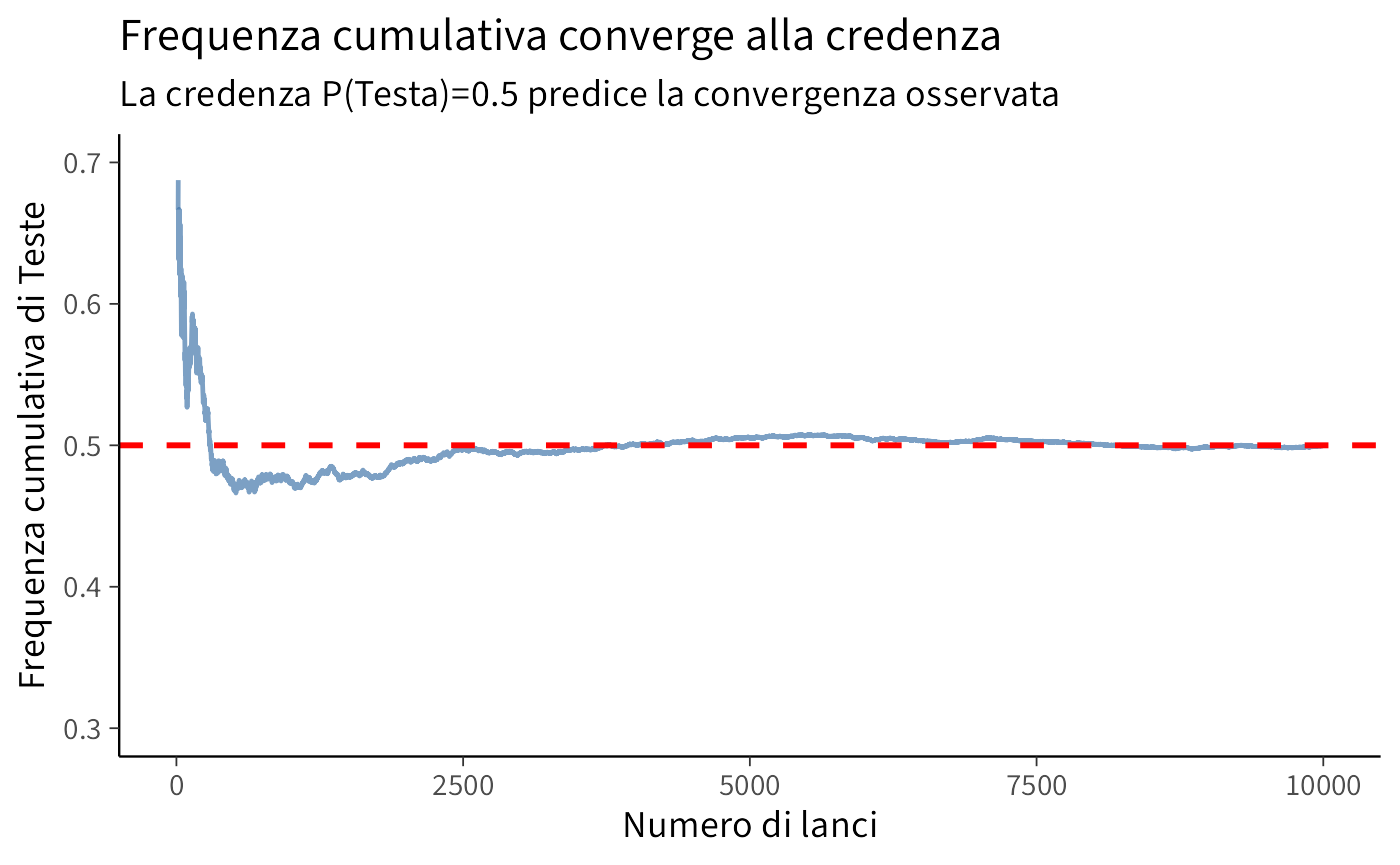
\includegraphics[width=0.85\linewidth,height=\textheight,keepaspectratio]{chapters/probability/01_intro_prob_bayesian_files/figure-pdf/unnamed-chunk-2-1.png}
\end{center}

L'interpretazione bayesiana di questa simulazione evidenzia che
l'assegnazione di \(P(\text{Testa}) = 0.5\) deriva da un principio di
simmetria epistemica, in assenza di informazioni che privilegino un
esito rispetto all'altro. La simulazione verifica la coerenza di questa
credenza con il comportamento empirico atteso. È importante notare che
la probabilità 0.5 non è definita dalla convergenza empirica, ma
rappresenta un'assegnazione a priori che la legge dei grandi numeri
successivamente conferma.

\section{Introduzione all'aggiornamento
bayesiano}\label{introduzione-allaggiornamento-bayesiano}

Uno dei principi fondamentali dell'epistemologia bayesiana stabilisce
che gli agenti razionali possiedono credenze di diversa intensità che
devono rispettare gli assiomi della probabilità. Lo stato di una
credenza e la sua evoluzione in seguito all'acquisizione di nuove
evidenze possono essere rappresentati tramite distribuzioni
probabilistiche.

\subsection{Il principio di
condizionalizzazione}\label{il-principio-di-condizionalizzazione}

Il \textbf{Principio di Condizionalizzazione} descrive come un agente
razionale dovrebbe aggiornare le proprie credenze alla luce di nuove
informazioni. Si basa sul concetto di probabilità condizionata: la
probabilità assegnata a un'ipotesi prima di ricevere l'evidenza, detta
\emph{a priori}, viene trasformata in una probabilità \emph{a
posteriori} una volta osservata l'informazione nuova.

Questo principio non è né un assioma formale né una definizione, ma un
\textbf{metodo operativo} che formalizza la dinamica della revisione
delle credenze. In termini concreti, se al tempo \(t\) la probabilità di
un'ipotesi \(H\) è \(P(H)\) e al tempo \(t' > t\) si osserva un'evidenza
\(E\), la credenza aggiornata in \(H\) deve corrispondere alla
probabilità a priori di \(H\) condizionata all'evidenza:

\[
P_{t'}(H) = P_t(H \mid E).
\]

In altre parole, condizionalizzare significa incorporare
sistematicamente le nuove informazioni senza contraddire le credenze
pregresse, garantendo coerenza interna nel processo di aggiornamento in
condizioni di incertezza.

\subsection{Il teorema di Bayes}\label{il-teorema-di-bayes}

Il teorema di Bayes fornisce il quadro formale per effettuare tale
aggiornamento:

\[
P(H \mid E) = \frac{P(E \mid H) \, P(H)}{P(E)}.
\]

La formula definisce la \emph{probabilità a posteriori} \(P(H \mid E)\)
dell'ipotesi \(H\) data l'evidenza \(E\) come funzione di tre
componenti: la \emph{probabilità a priori} \(P(H)\), che esprime la
credenza iniziale nell'ipotesi; la \emph{verosimiglianza}
\(P(E \mid H)\), che quantifica la probabilità di osservare l'evidenza
\(E\) nell'ipotesi che \(H\) sia vera; e la \emph{probabilità marginale
dell'evidenza} \(P(E)\), che rappresenta la probabilità complessiva di
osservare \(E\) indipendentemente dalla verità di \(H\).

\subsubsection{Applicazione ai test
diagnostici}\label{applicazione-ai-test-diagnostici}

Un esempio immediato di aggiornamento bayesiano si trova
nell'interpretazione dei risultati di un \textbf{test diagnostico}. In
questo contesto, l'ipotesi \(H\) corrisponde tipicamente alla presenza
della malattia \(D\), mentre l'evidenza \(E\) è rappresentata da un
risultato positivo del test (\(+\)).

La \textbf{probabilità a priori} \(P(D)\) riflette la prevalenza della
malattia nella popolazione di riferimento. La \textbf{verosimiglianza}
\(P(+ \mid D)\) corrisponde alla sensibilità del test, ovvero alla
probabilità di ottenere un risultato positivo in chi è effettivamente
malato, mentre \(P(+ \mid \neg D)\) rappresenta il tasso di falsi
positivi.

Il \textbf{teorema di Bayes} permette di combinare queste informazioni
per ottenere la probabilità a posteriori di malattia, dato un risultato
positivo:

\[
P(D \mid +) =
\frac{P(+ \mid D) , P(D)}
{P(+ \mid D) , P(D) + P(+ \mid \neg D) , P(\neg D)}.
\]

In questo modo, l'aggiornamento bayesiano integra le caratteristiche
intrinseche del test con il contesto epidemiologico, fornendo una stima
quantitativa rigorosa della probabilità che un individuo sia realmente
malato dopo aver ottenuto un risultato positivo. Questo esempio mostra
come il ragionamento bayesiano renda esplicita e formalmente coerente la
combinazione di informazioni empiriche e conoscenze pregresse.

\paragraph{Implementazione numerica}\label{implementazione-numerica}

Per fare un esempio, consideriamo uno scenario diagnostico con
prevalenza \(P(D) = 0.10\), sensibilità \(P(+ \mid D) = 0.80\) e
specificità \(P(- \mid \neg D) = 0.90\) (da cui un tasso di falsi
positivi \(P(+ \mid \neg D) = 0.10\)).

\begin{Shaded}
\begin{Highlighting}[]
\CommentTok{\# Parametri del test}
\NormalTok{p\_D   }\OtherTok{\textless{}{-}} \FloatTok{0.10}       \CommentTok{\# Prevalenza = prior P(D)}
\NormalTok{sens  }\OtherTok{\textless{}{-}} \FloatTok{0.80}       \CommentTok{\# Sensibilità = P(+ | D)}
\NormalTok{spec  }\OtherTok{\textless{}{-}} \FloatTok{0.90}       \CommentTok{\# Specificità = P({-} | \textasciitilde{}D)}
\NormalTok{p\_pos\_given\_notD }\OtherTok{\textless{}{-}} \DecValTok{1} \SpecialCharTok{{-}}\NormalTok{ spec  }\CommentTok{\# Falsi positivi P(+ | \textasciitilde{}D)}

\CommentTok{\# Probabilità complessiva di test positivo}
\NormalTok{p\_pos }\OtherTok{\textless{}{-}}\NormalTok{ sens }\SpecialCharTok{*}\NormalTok{ p\_D }\SpecialCharTok{+}\NormalTok{ p\_pos\_given\_notD }\SpecialCharTok{*}\NormalTok{ (}\DecValTok{1} \SpecialCharTok{{-}}\NormalTok{ p\_D)}

\CommentTok{\# Teorema di Bayes: posterior}
\NormalTok{p\_D\_given\_pos }\OtherTok{\textless{}{-}}\NormalTok{ (sens }\SpecialCharTok{*}\NormalTok{ p\_D) }\SpecialCharTok{/}\NormalTok{ p\_pos}

\FunctionTok{cat}\NormalTok{(}\StringTok{"P(D) ="}\NormalTok{, p\_D, }\StringTok{"}\SpecialCharTok{\textbackslash{}n}\StringTok{"}\NormalTok{)}
\CommentTok{\#\textgreater{} P(D) = 0.1}
\FunctionTok{cat}\NormalTok{(}\StringTok{"P(D | +) ="}\NormalTok{, }\FunctionTok{round}\NormalTok{(p\_D\_given\_pos, }\DecValTok{3}\NormalTok{), }\StringTok{"}\SpecialCharTok{\textbackslash{}n}\StringTok{"}\NormalTok{)}
\CommentTok{\#\textgreater{} P(D | +) = 0.471}
\end{Highlighting}
\end{Shaded}

L'aggiornamento delle conoscenze rivela che, nonostante il risultato
positivo del test, la probabilità a posteriori di essere malati è solo
del 47\%. Questo risultato controintuitivo si spiega con la bassa
prevalenza della malattia nella popolazione: il numero di falsi positivi
è così elevato da superare quello dei veri positivi.

\paragraph{Analisi tramite tabella di
contingenza}\label{analisi-tramite-tabella-di-contingenza}

La rappresentazione tramite tabella di contingenza per una popolazione
di 1000 individui chiarisce visivamente il risultato:

\begin{Shaded}
\begin{Highlighting}[]
\CommentTok{\# Costruzione della tabella di contingenza}
\NormalTok{N }\OtherTok{\textless{}{-}} \DecValTok{1000}
\NormalTok{malati }\OtherTok{\textless{}{-}}\NormalTok{ N }\SpecialCharTok{*}\NormalTok{ p\_D}
\NormalTok{sani }\OtherTok{\textless{}{-}}\NormalTok{ N }\SpecialCharTok{*}\NormalTok{ (}\DecValTok{1} \SpecialCharTok{{-}}\NormalTok{ p\_D)}

\NormalTok{veri\_positivi }\OtherTok{\textless{}{-}}\NormalTok{ malati }\SpecialCharTok{*}\NormalTok{ sens}
\NormalTok{falsi\_negativi }\OtherTok{\textless{}{-}}\NormalTok{ malati }\SpecialCharTok{*}\NormalTok{ (}\DecValTok{1} \SpecialCharTok{{-}}\NormalTok{ sens)}
\NormalTok{falsi\_positivi }\OtherTok{\textless{}{-}}\NormalTok{ sani }\SpecialCharTok{*}\NormalTok{ p\_pos\_given\_notD}
\NormalTok{veri\_negativi }\OtherTok{\textless{}{-}}\NormalTok{ sani }\SpecialCharTok{*}\NormalTok{ spec}

\NormalTok{tabella\_contingenza }\OtherTok{\textless{}{-}} \FunctionTok{data.frame}\NormalTok{(}
  \AttributeTok{Stato\_reale =} \FunctionTok{c}\NormalTok{(}\StringTok{"Malato (D)"}\NormalTok{, }\StringTok{"Sano (¬D)"}\NormalTok{, }\StringTok{"Totale"}\NormalTok{),}
  \AttributeTok{Positivo =} \FunctionTok{c}\NormalTok{(veri\_positivi, falsi\_positivi, veri\_positivi }\SpecialCharTok{+}\NormalTok{ falsi\_positivi),}
  \AttributeTok{Negativo =} \FunctionTok{c}\NormalTok{(falsi\_negativi, veri\_negativi, falsi\_negativi }\SpecialCharTok{+}\NormalTok{ veri\_negativi),}
  \AttributeTok{Totale =} \FunctionTok{c}\NormalTok{(malati, sani, N)}
\NormalTok{)}
\NormalTok{tabella\_contingenza}
\CommentTok{\#\textgreater{}   Stato\_reale Positivo Negativo Totale}
\CommentTok{\#\textgreater{} 1  Malato (D)       80       20    100}
\CommentTok{\#\textgreater{} 2   Sano (¬D)       90      810    900}
\CommentTok{\#\textgreater{} 3      Totale      170      830   1000}
\end{Highlighting}
\end{Shaded}

Tra i 170 test positivi, solo 80 (il 47\%) corrispondono a individui
effettivamente malati, mentre 90 (il 53\%) sono falsi positivi.

\subsubsection{Sintesi concettuale}\label{sintesi-concettuale}

Il processo di aggiornamento bayesiano può essere sintetizzato nel modo
seguente:

\[
\underbrace{P(D)}_{\text{prior}} \xrightarrow[\text{verosimiglianza e falsi positivi}]{\text{aggiornamento bayesiano}} \underbrace{P(D|+)}_{\text{posterior}}.
\]

Il teorema di Bayes dimostra che la probabilità finale dipende non solo
dalle caratteristiche del test, ma anche dalla plausibilità iniziale
dell'ipotesi. Dal punto di vista psicologico, questo rappresenta un
modello formale del ragionamento inferenziale che integra
sistematicamente le nuove informazioni con le conoscenze pregresse.

\section{Il ruolo della probabilità nello studio dei fenomeni
psicologici}\label{il-ruolo-della-probabilituxe0-nello-studio-dei-fenomeni-psicologici}

La teoria della probabilità bayesiana si rivela particolarmente adatta
alla psicologia, offrendo strumenti concettuali e metodologici che
rispondono alle esigenze specifiche della ricerca e della pratica
clinica.

\subsection{Quantificare l'incertezza
diagnostica}\label{quantificare-lincertezza-diagnostica}

La pratica clinica opera raramente in condizioni di certezza assoluta.
Il processo diagnostico richiede l'integrazione di molteplici fonti
informative, quali l'anamnesi, l'osservazione comportamentale e i test
psicometrici, ciascuna delle quali è caratterizzata da un proprio grado
di incertezza. Il framework bayesiano fornisce strumenti per
quantificare esplicitamente l'incertezza diagnostica e per aggiornare in
modo coerente le credenze del clinico con ogni nuova evidenza. Un
aspetto particolarmente significativo è la possibilità di incorporare
esplicitamente la prevalenza dei disturbi nella popolazione di
riferimento, prevenendo gli errori diagnostici derivanti dalla
negligenza dei tassi di base.

\subsection{Modellare processi
cognitivi}\label{modellare-processi-cognitivi}

Un programma di ricerca sempre più influente propone che la mente umana
operi secondo principi fondamentalmente bayesiani
(\citeproc{ref-griffiths2024bayesian}{Griffiths et al., 2024}). Nel
campo della percezione, le evidenze suggeriscono che il cervello integri
sistematicamente le aspettative pregresse con gli input sensoriali
attuali, in modo simile a quanto farebbe un osservatore bayesiano
ideale. Questo modello spiega i fenomeni delle illusioni percettive, in
cui aspettative robuste possono sovrascrivere segnali sensoriali
ambigui. L'apprendimento può essere concepito come un aggiornamento
bayesiano delle credenze attraverso l'esperienza, mentre molti bias
cognitivi documentati possono essere interpretati come deviazioni
sistematiche dall'ottimalità bayesiana.

\subsection{Analisi dei dati
sperimentali}\label{analisi-dei-dati-sperimentali}

Dal punto di vista metodologico, l'inferenza bayesiana offre diversi
vantaggi nell'analisi dei dati psicologici: consente di incorporare
formalmente le conoscenze pregresse attraverso distribuzioni a priori,
quantifica direttamente l'evidenza a favore dell'ipotesi nulla
(superando una limitazione del valore-\(p\)), gestisce in modo naturale
i piccoli campioni, e propaga l'incertezza in modo coerente attraverso
tutti i livelli dei modelli statistici complessi.

\subsection{Decisioni cliniche}\label{decisioni-cliniche}

In ambito terapeutico, l'approccio bayesiano supporta le decisioni
cliniche attraverso l'aggiornamento sequenziale delle stime di efficacia
terapeutica, a partire da evidenze generali sulla popolazione fino alle
risposte specifiche del singolo paziente. Questo processo iterativo
consente di modificare i protocolli terapeutici in risposta a nuove
evidenze e fornisce strumenti analitici per bilanciare probabilità e
utilità nelle scelte cliniche.

\section{Confronto con l'approccio
frequentista}\label{confronto-con-lapproccio-frequentista}

Per comprendere appieno la prospettiva bayesiana, è utile confrontarla
con l'approccio frequentista, evidenziandone le differenze fondamentali
già a livello di definizione della probabilità. Il \textbf{frequentismo}
interpreta la probabilità come il limite della frequenza relativa in una
serie infinita di prove ripetute, mentre il l'approccio
\textbf{bayesiano} la considera un \emph{grado di credenza razionale},
soggettivo ma formalmente coerente, assegnato a ipotesi o eventi
incerti.

Nel paradigma frequentista, i parametri di interesse sono
\textbf{quantità fisse}: non è possibile attribuire loro una probabilità
e l'inferenza si concentra sulle proprietà delle procedure di stima in
un gran numero di replicazioni. L'approccio bayesiano, al contrario,
considera i parametri come \emph{variabili casuali} dotate di
distribuzioni di probabilità che riflettono l'incertezza. Ciò consente
di formulare affermazioni probabilistiche dirette, come ad esempio: ``La
probabilità che l'effetto del trattamento sia positivo è 0.85''.

Una differenza cruciale riguarda gli \textbf{intervalli di stima}. Nel
frequentismo, un intervallo di confidenza al 95\% è costruito in modo
tale che, in un numero teoricamente infinito di replicazioni dello
stesso esperimento, il 95\% degli intervalli ottenuti conterrà il
parametro vero. Tuttavia, questa definizione \emph{non permette di
attribuire una probabilità a un intervallo specifico} basandosi sui dati
osservati. Al contrario, gli intervalli di credibilità bayesiani offrono
un'\emph{interpretazione probabilistica diretta}: dati i dati osservati,
possiamo affermare che esiste, per esempio, che esiste il 95\% di
probabilità che il parametro cada all'interno dell'intervallo, rendendo
l'inferenza immediatamente interpretabile per decisioni concrete.

Un altro elemento distintivo riguarda il \textbf{ruolo delle conoscenze
pregresse}. Il framework frequentista non fornisce un meccanismo formale
per integrarle, mentre l'approccio bayesiano le incorpora esplicitamente
attraverso la distribuzione a priori, rendendo trasparente il modo in
cui le informazioni precedenti influenzano le inferenze.

Infine, l'approccio frequentista fa ampio uso dei \textbf{valori-\(p\)},
che rispondono alla domanda: ``Quanto sarebbero sorprendenti i dati
osservati se l'ipotesi nulla fosse vera?'' Tuttavia, questa formulazione
spesso \emph{non corrisponde all'interrogativo scientifico effettivo},
cioè alla plausibilità dell'ipotesi alla luce dei dati. L'approccio
bayesiano, al contrario, consente di rispondere direttamente a questa
domanda centrale: ``Quanto è probabile che l'ipotesi nulla sia vera dato
ciò che abbiamo osservato?'', calcolando le \emph{probabilità a
posteriori} delle ipotesi e fornendo così una misura quantitativa di
credibilità razionale.

\section*{Riflessioni conclusive}\label{riflessioni-conclusive}

\markright{Riflessioni conclusive}

In questo capitolo abbiamo abbandonato la concezione della probabilità
come mera frequenza relativa, abbracciando la prospettiva della
probabilità come grado di credenza razionale. Questa visione, radicata
nella tradizione di Bayes, Laplace e de Finetti, non è solo un
tecnicismo matematico, ma una lente interpretativa che ci permette di
comprendere il ragionamento in condizioni di incertezza.

Gli assiomi della probabilità fungono da vincoli di coerenza logica per
le nostre convinzioni, principi di razionalità la cui violazione conduce
a contraddizioni. La prospettiva bayesiana consente di quantificare
l'incertezza anche per eventi unici e non ripetibili, come la prognosi
di un singolo paziente, senza dover ricorrere all'artificio di
esperimenti infinitamente replicati. Questo approccio garantisce
trasparenza, rendendo esplicite tutte le assunzioni iniziali codificate
nelle probabilità a priori e formalizzando matematicamente il processo
dinamico di apprendimento dall'esperienza attraverso il teorema di
Bayes.

Nei prossimi capitoli, svilupperemo gli strumenti formali di questo
quadro teorico. Scopriremo che concetti fondamentali come
l'equiprobabilità non sono proprietà intrinseche del mondo, ma il
riflesso di simmetrie nel nostro stato informativo. La probabilità
bayesiana non elimina l'incertezza, ma fornisce gli strumenti per
quantificarla e gestirla in modo razionale, rappresentando il suo
contributo più prezioso alla ricerca psicologica, ambito in cui
l'incertezza è la norma piuttosto che l'eccezione.

\section*{Bibliografia}\label{bibliografia}

\markright{Bibliografia}

\chapter{Assiomi e coerenza delle
credenze}\label{sec-prob-axioms-coherence}

\section*{Introduzione}\label{introduzione-2}

\markright{Introduzione}

Dopo aver introdotto la probabilità come \emph{grado di credenza
razionale} nel Chapter~\ref{sec-prob-interpretation}, il presente
capitolo sviluppa il quadro matematico per operare coerentemente con
tali credenze. Verrà esaminato come lo \emph{spazio campionario} e gli
\emph{eventi} rappresentino possibilità epistemiche, e come gli
\emph{assiomi di Kolmogorov} fungano da vincoli di coerenza logica per
le nostre assegnazioni probabilistiche.

Un aspetto centrale della trattazione concerne la costruzione e
manipolazione di \emph{tabelle di probabilità congiunta}, che
costituiscono lo strumento operativo fondamentale per rappresentare
credenze su sistemi complessi. Queste tabelle, in particolare nel caso
semplice 2×2, rendono esplicita la relazione tra probabilità
\emph{congiunte}, \emph{marginali} e \emph{condizionate}, dimostrando
come tutte le probabilità di interesse derivino da un'unica struttura
coerente.

Attraverso esempi tratti dalla psicologia e mediante simulazioni in R,
verranno illustrate metodologie per diagnosticare e correggere
incoerenze nelle assegnazioni probabilistiche, nonché per verificare
empiricamente come credenze coerenti generino i comportamenti attesi nei
dati osservati.

\subsection*{Panoramica del capitolo}\label{panoramica-del-capitolo-1}

\begin{itemize}
\tightlist
\item
  Spazio campionario ed eventi come possibilità epistemiche.
\item
  Assiomi di Kolmogorov come vincoli di coerenza.
\item
  Diagnosi di incoerenze: additività e vincoli di Fréchet.
\item
  Tabelle di probabilità congiunta (2×2 e oltre).
\item
  Derivazione di marginali e condizionate da congiunte.
\item
  Verifica empirica della coerenza con simulazioni.
\end{itemize}

\begin{tcolorbox}[enhanced jigsaw, arc=.35mm, breakable, colbacktitle=quarto-callout-tip-color!10!white, opacityback=0, toprule=.15mm, rightrule=.15mm, colback=white, opacitybacktitle=0.6, leftrule=.75mm, coltitle=black, bottomtitle=1mm, left=2mm, toptitle=1mm, title=\textcolor{quarto-callout-tip-color}{\faLightbulb}\hspace{0.5em}{Prerequisiti}, titlerule=0mm, bottomrule=.15mm, colframe=quarto-callout-tip-color-frame]

\begin{itemize}
\tightlist
\item
  Aver letto il Chapter~\ref{sec-prob-interpretation}.
\item
  Leggere l'Appendix~\ref{sec-apx-sets} (teoria degli insiemi).
\item
  Familiarità base con R e ggplot2.
\end{itemize}

\end{tcolorbox}

\begin{tcolorbox}[enhanced jigsaw, arc=.35mm, breakable, colbacktitle=quarto-callout-caution-color!10!white, opacityback=0, toprule=.15mm, rightrule=.15mm, colback=white, opacitybacktitle=0.6, leftrule=.75mm, coltitle=black, bottomtitle=1mm, left=2mm, toptitle=1mm, title=\textcolor{quarto-callout-caution-color}{\faFire}\hspace{0.5em}{Preparazione del Notebook}, titlerule=0mm, bottomrule=.15mm, colframe=quarto-callout-caution-color-frame]

\begin{Shaded}
\begin{Highlighting}[]
\NormalTok{here}\SpecialCharTok{::}\FunctionTok{here}\NormalTok{(}\StringTok{"code"}\NormalTok{, }\StringTok{"\_common.R"}\NormalTok{) }\SpecialCharTok{|\textgreater{}} 
  \FunctionTok{source}\NormalTok{()}

\CommentTok{\# Load packages}
\ControlFlowTok{if}\NormalTok{ (}\SpecialCharTok{!}\FunctionTok{requireNamespace}\NormalTok{(}\StringTok{"pacman"}\NormalTok{)) }\FunctionTok{install.packages}\NormalTok{(}\StringTok{"pacman"}\NormalTok{)}
\NormalTok{pacman}\SpecialCharTok{::}\FunctionTok{p\_load}\NormalTok{(ggplot2, dplyr, tidyr, viridis)}
\end{Highlighting}
\end{Shaded}

\end{tcolorbox}

\section{Spazio campionario come possibilità
epistemiche}\label{spazio-campionario-come-possibilituxe0-epistemiche}

Nel linguaggio probabilistico classico, lo spazio campionario \(\Omega\)
viene definito come l'insieme di tutti gli esiti possibili di un
esperimento casuale. Nell'approccio bayesiano, questa definizione
richiede una rilettura in chiave epistemica.

\begin{definition}[Spazio campionario (visione
bayesiana)]\protect\hypertarget{def-sample-space-bayesian}{}\label{def-sample-space-bayesian}

Lo \emph{spazio campionario} \(\Omega\) rappresenta l'insieme delle
\emph{possibilità epistemiche} compatibili con lo stato attuale delle
informazioni disponibili. Esso non descrive necessariamente ciò che può
accadere fisicamente, ma piuttosto ciò che, dati i limiti della nostra
conoscenza attuale, consideriamo logicamente possibile.

\end{definition}

\subsection{Caratteristiche dello spazio campionario
epistemico}\label{caratteristiche-dello-spazio-campionario-epistemico}

Lo spazio campionario epistemico presenta caratteristiche distintive che
riflettono la natura soggettiva e informazionale della probabilità
bayesiana. La sua composizione dipende criticamente dall'informazione
disponibile e può modificarsi in seguito all'acquisizione di nuove
evidenze. Ad esempio, prima di osservare l'esito di un test diagnostico,
lo spazio campionario comprende i valori ``positivo'' e ``negativo'';
successivamente all'osservazione di un risultato positivo, lo spazio si
riduce di conseguenza.

La definizione dello spazio campionario non è univoca: ricercatori
diversi, con informazioni diverse o con assunzioni diverse, possono
legittimamente definire spazi campionari diversi per lo stesso fenomeno.
La costruzione di \(\Omega\) richiede infine la specificazione attenta
del livello di dettaglio rilevante per la particolare domanda di
ricerca, riflettendo un bilanciamento tra completezza descrittiva e
pertinenza analitica.

\begin{tcolorbox}[enhanced jigsaw, arc=.35mm, breakable, colbacktitle=quarto-callout-note-color!10!white, opacityback=0, toprule=.15mm, rightrule=.15mm, colback=white, opacitybacktitle=0.6, leftrule=.75mm, coltitle=black, bottomtitle=1mm, left=2mm, toptitle=1mm, title=\textcolor{quarto-callout-note-color}{\faInfo}\hspace{0.5em}{Esempio psicologico}, titlerule=0mm, bottomrule=.15mm, colframe=quarto-callout-note-color-frame]

\subsection*{Spazio campionario per una valutazione
clinica}\label{spazio-campionario-per-una-valutazione-clinica}

Consideriamo la valutazione di un paziente per possibile depressione. Lo
spazio campionario può essere definito in modi diversi a seconda delle
informazioni e degli obiettivi:

\textbf{Livello 1 (binario):}
\[\Omega_1 = \{\text{Depresso}, \text{Non depresso}\}.\]

\textbf{Livello 2 (severità):}
\[\Omega_2 = \{\text{Nessuna}, \text{Lieve}, \text{Moderata}, \text{Severa}\}.\]

\textbf{Livello 3 (combinazioni):}
\[\Omega_3 = \{\text{Depressione}, \text{Ansia}, \text{Comorbidità}, \text{Nessuna}\}.\]

La scelta dipende da:

\begin{itemize}
\tightlist
\item
  informazioni disponibili (screening, test, colloquio);
\item
  obiettivo clinico (screening vs diagnosi differenziale);
\item
  decisioni da prendere (trattamento, monitoraggio).
\end{itemize}

Ogni spazio è legittimo nel proprio contesto. La probabilità assegnata
riflette la credenza in quello specifico spazio.

\end{tcolorbox}

\section{Eventi come proposizioni sul
mondo}\label{eventi-come-proposizioni-sul-mondo}

Nella prospettiva bayesiana, un \emph{evento} rappresenta un
sottoinsieme di \(\Omega\) che corrisponde a una \emph{proposizione} sul
mondo, suscettibile di essere vera o falsa.

\begin{definition}[Evento]\protect\hypertarget{def-event-bayesian}{}\label{def-event-bayesian}

Un \emph{evento} \(A \subseteq \Omega\) costituisce una
\emph{proposizione} sul mondo alla quale possiamo assegnare un grado di
credenza \(P(A)\), condizionato allo stato informativo corrente.

\end{definition}

\subsection{Operazioni su eventi}\label{operazioni-su-eventi}

Le operazioni insiemistiche tradizionali possiedono interpretazioni
epistemiche naturali nel contesto bayesiano. L'\emph{unione}
\(A \cup B\) corrisponde all'affermazione che ``la proposizione \(A\)
oppure la proposizione \(B\) è vera''. L'\emph{intersezione}
\(A \cap B\) rappresenta la situazione in cui ``entrambe le proposizioni
\(A\) e \(B\) sono vere''. Il \emph{complemento} \(A^c\) esprime la
negazione ``la proposizione \(A\) non è vera''.

L'\emph{insieme vuoto} \(\varnothing\) identifica una proposizione
logicamente contraddittoria, necessariamente falsa per vincoli logici.
Lo \emph{spazio campionario} \(\Omega\) rappresenta invece una
proposizione logicamente vera, affermando che qualcosa accade
all'interno dell'insieme delle possibilità epistemiche definite.

\begin{tcolorbox}[enhanced jigsaw, arc=.35mm, breakable, colbacktitle=quarto-callout-note-color!10!white, opacityback=0, toprule=.15mm, rightrule=.15mm, colback=white, opacitybacktitle=0.6, leftrule=.75mm, coltitle=black, bottomtitle=1mm, left=2mm, toptitle=1mm, title=\textcolor{quarto-callout-note-color}{\faInfo}\hspace{0.5em}{Esempio: Eventi in un test psicometrico}, titlerule=0mm, bottomrule=.15mm, colframe=quarto-callout-note-color-frame]

\subsection{Proposizioni nella Satisfaction with Life Scale
(SWLS)}\label{proposizioni-nella-satisfaction-with-life-scale-swls}

La SWLS ha punteggi che vanno da 5 a 35. Definiamo:

\begin{itemize}
\tightlist
\item
  \(\Omega = \{5, 6, 7, \ldots, 35\}\) (possibili punteggi).
\item
  \(A =\) ``Punteggio ≥ 25'' (alta soddisfazione)
  \(= \{25, 26, \ldots, 35\}\).
\item
  \(B =\) ``Punteggio ≤ 15'' (bassa soddisfazione)
  \(= \{5, 6, \ldots, 15\}\).
\item
  \(C =\) ``Punteggio tra 16 e 24'' (soddisfazione moderata)
  \(= \{16, 17, \ldots, 24\}\).
\end{itemize}

Operazioni:

\begin{itemize}
\tightlist
\item
  \(A \cup B\): ``Soddisfazione alta \emph{o} bassa'' (non moderata).
\item
  \(A \cap B = \varnothing\): proposizioni mutualmente esclusive
  (impossibile avere entrambi).
\item
  \(A^c = B \cup C\): ``Non alta soddisfazione''.
\item
  \(A \cup B \cup C = \Omega\): proposizioni esaustive.
\end{itemize}

La credenza \(P(A)\) quantifica quanto riteniamo plausibile, in base a
ciò che sappiamo (popolazione, contesto), che un individuo scelto abbia
un'alta soddisfazione.

\end{tcolorbox}

\section{Gli assiomi di Kolmogorov come vincoli di
coerenza}\label{gli-assiomi-di-kolmogorov-come-vincoli-di-coerenza}

Nel Chapter~\ref{sec-prob-interpretation} abbiamo visto che gli assiomi
di Kolmogorov non sono leggi naturali ma vincoli per evitare incoerenze
(il cosiddetto \emph{Dutch Book}). Qui li formalizziamo e approfondiamo
le loro implicazioni.

\begin{definition}[Funzione di probabilità (definizione
bayesiana)]\protect\hypertarget{def-probability-measure}{}\label{def-probability-measure}

Una \emph{funzione di probabilità} \(P: \mathcal{F} \to [0,1]\) assegna
a ogni evento \(A\) in una famiglia di eventi \(\mathcal{F}\) un numero
\(P(A)\) che rappresenta il grado di credenza nell'affermazione \(A\).
Per essere coerente, \(P\) deve soddisfare i seguenti \emph{assiomi di
coerenza}:

\begin{enumerate}
\def\labelenumi{\arabic{enumi}.}
\item
  \textbf{Non-negatività}: \(P(A) \geq 0\) per ogni evento \(A\).
\item
  \textbf{Normalizzazione}: \(P(\Omega) = 1\).
\item
  \textbf{Additività finita}: se \(A\) e \(B\) sono eventi disgiunti
  (\(A \cap B = \varnothing\)), allora \[P(A \cup B) = P(A) + P(B).\]
\item
  \textbf{Additività numerabile} (per spazi infiniti): se
  \(A_1, A_2, \ldots\) è una sequenza di eventi mutuamente disgiunti,
  allora
  \[P\left(\bigcup_{i=1}^{\infty} A_i\right) = \sum_{i=1}^{\infty} P(A_i).\]
\end{enumerate}

\end{definition}

\subsection{Interpretazione epistemica degli
assiomi}\label{interpretazione-epistemica-degli-assiomi}

La non negatività riflette l'impossibilità di un grado di credenza
negativo, dove lo 0 corrisponde a ``impossibile, dato lo stato
informativo attuale'' e l'1 a ``certo, dato lo stato informativo
attuale''. La normalizzazione esprime la certezza che almeno una delle
possibilità epistemiche nello spazio campionario si realizzi. Un valore
\(P(\Omega) < 1\) implicherebbe incoerentemente la possibilità che
nessuna delle opzioni considerate si verifichi. L'additività stabilisce
che, per affermazioni mutualmente esclusive, la credenza nella loro
disgiunzione deve equivalere alla somma delle credenze individuali; la
violazione di questo principio rende possibile la costruzione di un
\emph{Dutch book}.

\subsection{Conseguenze immediate degli
assiomi}\label{conseguenze-immediate-degli-assiomi}

Dagli assiomi fondamentali discendono diverse proprietà derivate di
notevole utilità pratica.

\begin{theorem}[Proprietà derivate della
probabilità]\protect\hypertarget{thm-probability-properties}{}\label{thm-probability-properties}

~

\begin{enumerate}
\def\labelenumi{\arabic{enumi}.}
\tightlist
\item
  \textbf{Probabilità del complemento}: \(P(A^c) = 1 - P(A)\).
\item
  \textbf{Probabilità dell'insieme vuoto}: \(P(\varnothing) = 0\).
\item
  \textbf{Monotonia (della probabilità)}: se \(A \subseteq B\), allora
  \(P(A) \leq P(B)\).
\item
  \textbf{Regola dell'unione} (eventi non disgiunti):
  \[P(A \cup B) = P(A) + P(B) - P(A \cap B).\]
\item
  \textbf{Principio di inclusione-esclusione} (generalizzazione):
  \[P(A_1 \cup A_2 \cup A_3) = \sum P(A_i) - \sum P(A_i \cap A_j) + P(A_1 \cap A_2 \cap A_3).\]
\end{enumerate}

\end{theorem}

Queste proprietà non costituiscono assiomi aggiuntivi, ma emergono come
conseguenze logiche necessarie dei tre assiomi di base. Una volta
accettati i vincoli di coerenza fondamentali, l'intero edificio della
teoria della probabilità si sviluppa in modo deduttivo.

\section{Diagnosi di incoerenze: casi
tipici}\label{diagnosi-di-incoerenze-casi-tipici}

Esaminiamo come identificare e correggere le incoerenze più frequenti
nelle assegnazioni probabilistiche.

\subsection{Incoerenza 1: violazione
dell'additività}\label{incoerenza-1-violazione-delladditivituxe0}

L'errore più comune consiste nel violare il principio di additività per
eventi disgiunti, assegnando una probabilità complessiva superiore a
quanto logicamente possibile.

\begin{tcolorbox}[enhanced jigsaw, arc=.35mm, breakable, colbacktitle=quarto-callout-warning-color!10!white, opacityback=0, toprule=.15mm, rightrule=.15mm, colback=white, opacitybacktitle=0.6, leftrule=.75mm, coltitle=black, bottomtitle=1mm, left=2mm, toptitle=1mm, title=\textcolor{quarto-callout-warning-color}{\faExclamationTriangle}\hspace{0.5em}{Esempio di incoerenza clinica}, titlerule=0mm, bottomrule=.15mm, colframe=quarto-callout-warning-color-frame]

\subsubsection*{Sovrastima delle
probabilità}\label{sovrastima-delle-probabilituxe0}

Un clinico valuta un paziente con sintomi psicotici e assegna i seguenti
gradi di credenza a tre diagnosi mutualmente esclusive:

\begin{itemize}
\tightlist
\item
  \(P(\text{Schizofrenia}) = 0.6\);
\item
  \(P(\text{Disturbo Bipolare}) = 0.5\);\\
\item
  \(P(\text{Nessun disturbo psicotico}) = 0.2\).
\end{itemize}

La somma \(0.6 + 0.5 + 0.2 = 1.3\) eccede il valore massimo consentito
di 1.

Questa assegnazione risulta incoerente poiché i tre eventi sono:

\begin{itemize}
\tightlist
\item
  \emph{mutualmente esclusivi}: il paziente può ricevere solo una delle
  tre diagnosi;
\item
  \emph{collettivamente esaustivi}: coprono tutti gli esiti diagnostici
  possibili.
\end{itemize}

Il clinico ha quindi attribuito più credenza (1.3) di quanta fosse
disponibile (1.0), come se possedesse il 130\% di certezza invece del
100\%.

\end{tcolorbox}

\subsection{Incoerenza 2: violazione dei vincoli di Fréchet per
congiunzioni di
eventi}\label{incoerenza-2-violazione-dei-vincoli-di-fruxe9chet-per-congiunzioni-di-eventi}

Quando consideriamo due eventi che possono verificarsi congiuntamente,
la probabilità della loro intersezione \(P(A \cap B)\) non può essere
assegnata liberamente, ma deve rispettare precisi vincoli matematici
derivanti dalla struttura logica della probabilità.

\begin{theorem}[Vincoli di
Fréchet]\protect\hypertarget{thm-frechet-bounds}{}\label{thm-frechet-bounds}

Per qualsiasi coppia di eventi \(A\) e \(B\) vale la disuguaglianza:

\[
\max\{0,\, P(A) + P(B) - 1\} \;\leq\; P(A \cap B) \;\leq\; \min\{P(A), P(B)\}.
\]

\textbf{Interpretazione intuitiva:}

Il limite superiore stabilisce che l'evento congiunto ``\(A\) e \(B\)
insieme'' non può essere più probabile dell'evento singolo meno
probabile tra \(A\) e \(B\). Il limite inferiore indica che quando la
somma delle probabilità individuali supera 1, allora \(A\) e \(B\)
devono necessariamente sovrapporsi almeno in parte.

\end{theorem}

\begin{tcolorbox}[enhanced jigsaw, arc=.35mm, breakable, colbacktitle=quarto-callout-note-color!10!white, opacityback=0, toprule=.15mm, rightrule=.15mm, colback=white, opacitybacktitle=0.6, leftrule=.75mm, coltitle=black, bottomtitle=1mm, left=2mm, toptitle=1mm, title=\textcolor{quarto-callout-note-color}{\faInfo}\hspace{0.5em}{Esempio clinico: Depressione e Ansia}, titlerule=0mm, bottomrule=.15mm, colframe=quarto-callout-note-color-frame]

\subsubsection*{Applicazione alla comorbidità
psicologica}\label{applicazione-alla-comorbidituxe0-psicologica}

Consideriamo uno studio su una popolazione clinica in cui la probabilità
di depressione è \(P(\text{Depressione}) = 0.6\) e la probabilità di
ansia è \(P(\text{Ansia}) = 0.5\). I vincoli di Fréchet determinano
l'intervallo di valori logicamente possibili per la comorbidità
\(P(\text{Depressione} \cap \text{Ansia})\).

Il limite inferiore risulta \(\max(0, 0.6 + 0.5 - 1) = 0.1\), mentre il
limite superiore è \(\min(0.6, 0.5) = 0.5\). Pertanto, l'intervallo
ammissibile per la probabilità di comorbidità è compreso tra 0.1 e 0.5.

Questa delimitazione ha implicazioni pratiche immediate: sarebbe
logicamente incoerente affermare che solo il 5\% della popolazione
presenta comorbidità, così come sarebbe incoerente sostenere che il 60\%
mostra comorbidità. Qualsiasi valore compreso tra il 10\% e il 50\%
risulta invece logicamente possibile.

\end{tcolorbox}

\subsection{Mappa dei valori
ammissibili}\label{mappa-dei-valori-ammissibili}

\begin{Shaded}
\begin{Highlighting}[]
\CommentTok{\# Creare griglia di valori}
\NormalTok{grid }\OtherTok{\textless{}{-}} \FunctionTok{expand.grid}\NormalTok{(}
  \AttributeTok{P\_A =} \FunctionTok{seq}\NormalTok{(}\DecValTok{0}\NormalTok{, }\DecValTok{1}\NormalTok{, }\AttributeTok{by =} \FloatTok{0.02}\NormalTok{),}
  \AttributeTok{P\_B =} \FunctionTok{seq}\NormalTok{(}\DecValTok{0}\NormalTok{, }\DecValTok{1}\NormalTok{, }\AttributeTok{by =} \FloatTok{0.02}\NormalTok{)}
\NormalTok{)}

\CommentTok{\# Calcolare vincoli per ogni coppia}
\NormalTok{grid}\SpecialCharTok{$}\NormalTok{limite\_inferiore }\OtherTok{\textless{}{-}} \FunctionTok{pmax}\NormalTok{(}\DecValTok{0}\NormalTok{, grid}\SpecialCharTok{$}\NormalTok{P\_A }\SpecialCharTok{+}\NormalTok{ grid}\SpecialCharTok{$}\NormalTok{P\_B }\SpecialCharTok{{-}} \DecValTok{1}\NormalTok{)}
\NormalTok{grid}\SpecialCharTok{$}\NormalTok{limite\_superiore }\OtherTok{\textless{}{-}} \FunctionTok{pmin}\NormalTok{(grid}\SpecialCharTok{$}\NormalTok{P\_A, grid}\SpecialCharTok{$}\NormalTok{P\_B)}
\NormalTok{grid}\SpecialCharTok{$}\NormalTok{ampiezza\_lecita }\OtherTok{\textless{}{-}}\NormalTok{ grid}\SpecialCharTok{$}\NormalTok{limite\_superiore }\SpecialCharTok{{-}}\NormalTok{ grid}\SpecialCharTok{$}\NormalTok{limite\_inferiore}

\CommentTok{\# Visualizzazione}
\FunctionTok{ggplot}\NormalTok{(grid, }\FunctionTok{aes}\NormalTok{(}\AttributeTok{x =}\NormalTok{ P\_A, }\AttributeTok{y =}\NormalTok{ P\_B, }\AttributeTok{fill =}\NormalTok{ ampiezza\_lecita)) }\SpecialCharTok{+}
  \FunctionTok{geom\_tile}\NormalTok{() }\SpecialCharTok{+}
  \FunctionTok{scale\_fill\_viridis\_c}\NormalTok{(}
    \AttributeTok{name =} \StringTok{"Ampiezza dell\textquotesingle{}intervallo}\SpecialCharTok{\textbackslash{}n}\StringTok{ammissibile"}\NormalTok{,}
    \AttributeTok{option =} \StringTok{"plasma"}\NormalTok{,}
    \AttributeTok{limits =} \FunctionTok{c}\NormalTok{(}\DecValTok{0}\NormalTok{, }\DecValTok{1}\NormalTok{)}
\NormalTok{  ) }\SpecialCharTok{+}
  \FunctionTok{labs}\NormalTok{(}
    \AttributeTok{title =} \StringTok{"Vincoli di Fréchet: intervalli ammissibili per P(A ∩ B)"}\NormalTok{,}
    \AttributeTok{subtitle =} \StringTok{"Per ogni coppia (P(A), P(B)), l\textquotesingle{}area colorata mostra quanti valori di P(A ∩ B) }\SpecialCharTok{\textbackslash{}n}\StringTok{sono logicamente possibili"}\NormalTok{,}
    \AttributeTok{x =} \StringTok{"P(A)"}\NormalTok{,}
    \AttributeTok{y =} \StringTok{"P(B)"}\NormalTok{,}
    \AttributeTok{caption =} \StringTok{"Colori più chiari = maggiore libertà nella scelta di P(A ∩ B)"}
\NormalTok{  ) }\SpecialCharTok{+}
  \FunctionTok{theme\_minimal}\NormalTok{() }\SpecialCharTok{+}
  \FunctionTok{coord\_fixed}\NormalTok{()}
\end{Highlighting}
\end{Shaded}

\begin{figure}[H]

{\centering 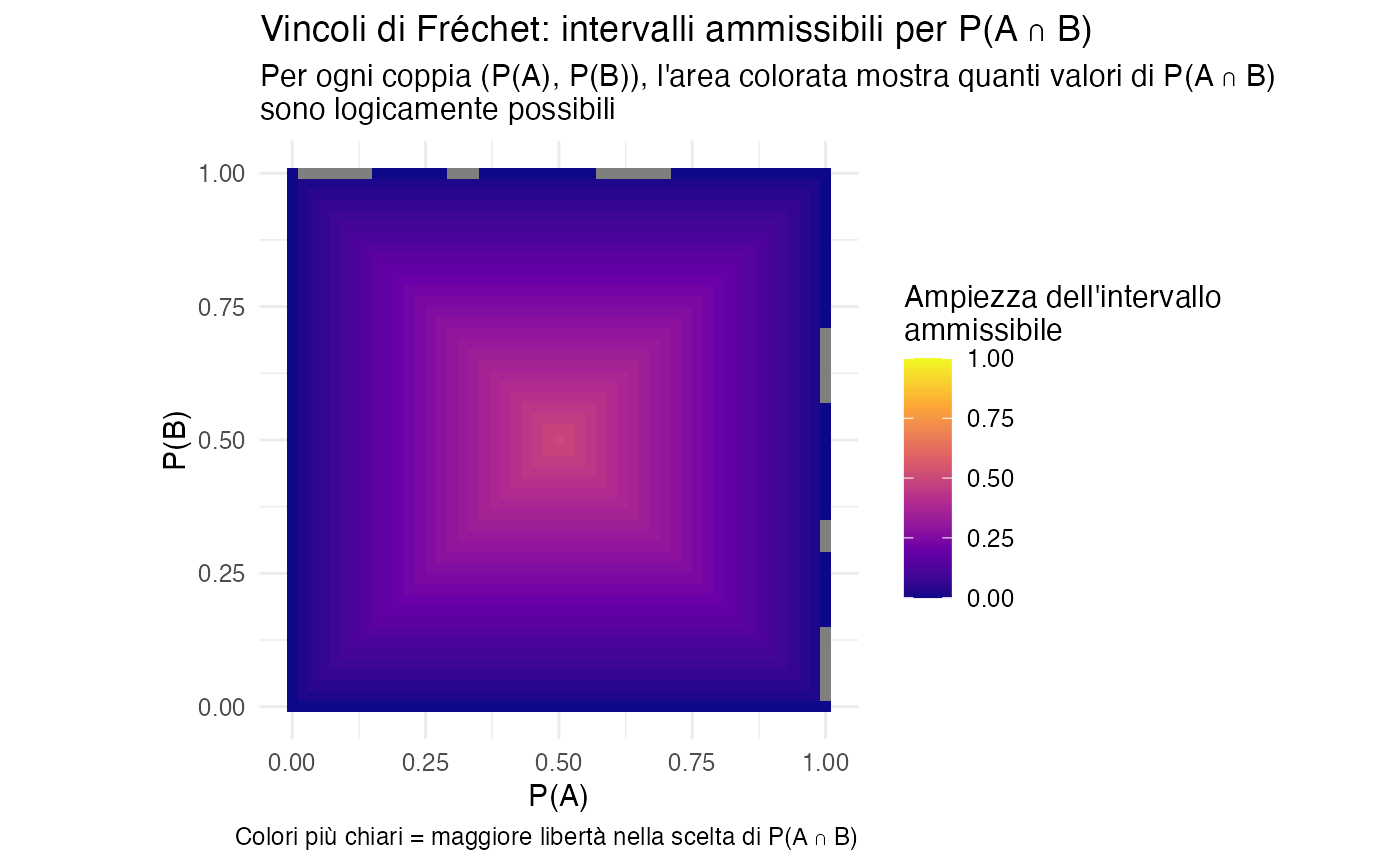
\includegraphics[width=0.8\linewidth,height=\textheight,keepaspectratio]{chapters/probability/02_axioms_coherence_bayesian_files/figure-pdf/unnamed-chunk-2-1.png}

}

\caption{Regione dei valori ammissibili per P(A ∩ B) in funzione di P(A)
e P(B).}

\end{figure}%

La mappa visualizza la relazione tra le probabilità marginali e
l'ampiezza dell'intervallo ammissibile per la loro intersezione. Le
regioni in blu scuro, corrispondenti agli angoli del quadrato unitario,
indicano vincoli particolarmente stringenti che limitano fortemente i
valori possibili per \(P(A \cap B)\). Al contrario, le regioni in
giallo, situate verso il centro della mappa, segnalano la massima
libertà nella scelta della probabilità dell'intersezione.

Nella regione in alto a destra, dove \(P(A) + P(B) > 1\), esiste una
sovrapposizione minima obbligatoria tra gli eventi. Nella regione in
basso a sinistra, dove \(P(A) + P(B) \leq 1\), la sovrapposizione può
teoricamente essere nulla.

Questi vincoli matematici offrono una protezione formale contro
l'assegnazione di probabilità logicamente impossibili a sintomi che si
presentano insieme o a condizioni psicologiche che co-occorrono,
risultando particolarmente utili nella pratica clinica e nella ricerca
psicometrica.

\section{Tabelle di probabilità
congiunta}\label{tabelle-di-probabilituxe0-congiunta}

Le \textbf{tabelle di probabilità congiunta} consentono di rappresentare
sistematicamente l'intero sistema di credenze relative a un fenomeno
caratterizzato da molteplici eventi. Tali tabelle rendono esplicite
tutte le possibili combinazioni degli esiti e costituiscono la base da
cui emergono coerentemente le probabilità marginali, quelle condizionate
e le relazioni di indipendenza statistica.

\subsection{Struttura di una tabella
2×2}\label{struttura-di-una-tabella-22}

Consideriamo due eventi dicotomici \(A\) e \(B\). La loro distribuzione
congiunta trova rappresentazione in una tabella 2×2 che organizza le
probabilità secondo la seguente struttura:

\begin{longtable}[]{@{}llll@{}}
\toprule\noalign{}
& \(B\) & \(B^c\) & Marginale \\
\midrule\noalign{}
\endhead
\bottomrule\noalign{}
\endlastfoot
\(A\) & \(P(A \cap B)\) & \(P(A \cap B^c)\) & \(P(A)\) \\
\(A^c\) & \(P(A^c \cap B)\) & \(P(A^c \cap B^c)\) & \(P(A^c)\) \\
\textbf{Marginale} & \(P(B)\) & \(P(B^c)\) & \(1\) \\
\end{longtable}

Le celle interne della tabella contengono le quattro probabilità
congiunte che specificano il grado di credenza in ciascuna combinazione
di eventi. Le probabilità marginali, collocate sui bordi della tabella,
si ottengono mediante la somma lungo le righe e le colonne: \(P(A)\) è
uguale alla somma \(P(A\cap B) + P(A\cap B^c)\), mentre \(P(B)\) deriva
da \(P(A\cap B) + P(A^c\cap B)\).

La coerenza complessiva della distribuzione è garantita dal vincolo di
normalizzazione che impone che la somma di tutte le probabilità
congiunte sia pari a 1. Una volta stabilita una tabella congiunta
coerente, tutte le ulteriori quantità probabilistiche di interesse
diventano accessibili attraverso operazioni algebriche elementari di
somma e normalizzazione.

\begin{tcolorbox}[enhanced jigsaw, arc=.35mm, breakable, colbacktitle=quarto-callout-note-color!10!white, opacityback=0, toprule=.15mm, rightrule=.15mm, colback=white, opacitybacktitle=0.6, leftrule=.75mm, coltitle=black, bottomtitle=1mm, left=2mm, toptitle=1mm, title=\textcolor{quarto-callout-note-color}{\faInfo}\hspace{0.5em}{Esempio di costruzione di una tabella di probabilità congiunta 2×2}, titlerule=0mm, bottomrule=.15mm, colframe=quarto-callout-note-color-frame]

\subsubsection*{Definizione dello
scenario}\label{definizione-dello-scenario}

Consideriamo un test diagnostico per la depressione caratterizzato da
due variabili dicotomiche: lo stato reale del paziente (\(D\) per
depresso, \(D^c\) per non depresso) e l'esito del test (\(T^+\) per
positivo, \(T^-\) per negativo). I parametri noti dalla letteratura
clinica includono una prevalenza della depressione \(P(D) = 0.15\), una
sensibilità del test \(P(T^+ \mid D) = 0.85\), e un tasso di falsi
positivi \(P(T^+ \mid D^c) = 0.20\).

\textbf{Costruzione della tabella di probabilità congiunta:}

\begin{Shaded}
\begin{Highlighting}[]
\CommentTok{\# Parametri di base}
\NormalTok{prevalenza }\OtherTok{\textless{}{-}} \FloatTok{0.15}
\NormalTok{sensibilita }\OtherTok{\textless{}{-}} \FloatTok{0.85}
\NormalTok{tasso\_falsi\_positivi }\OtherTok{\textless{}{-}} \FloatTok{0.20}

\CommentTok{\# Calcolo delle probabilità congiunte}
\NormalTok{p\_depresso\_positivo }\OtherTok{\textless{}{-}}\NormalTok{ sensibilita }\SpecialCharTok{*}\NormalTok{ prevalenza}
\NormalTok{p\_depresso\_negativo }\OtherTok{\textless{}{-}}\NormalTok{ (}\DecValTok{1} \SpecialCharTok{{-}}\NormalTok{ sensibilita) }\SpecialCharTok{*}\NormalTok{ prevalenza}
\NormalTok{p\_non\_depresso\_positivo }\OtherTok{\textless{}{-}}\NormalTok{ tasso\_falsi\_positivi }\SpecialCharTok{*}\NormalTok{ (}\DecValTok{1} \SpecialCharTok{{-}}\NormalTok{ prevalenza)}
\NormalTok{p\_non\_depresso\_negativo }\OtherTok{\textless{}{-}}\NormalTok{ (}\DecValTok{1} \SpecialCharTok{{-}}\NormalTok{ tasso\_falsi\_positivi) }\SpecialCharTok{*}\NormalTok{ (}\DecValTok{1} \SpecialCharTok{{-}}\NormalTok{ prevalenza)}

\CommentTok{\# Creazione della tabella}
\NormalTok{tabella\_congiunta }\OtherTok{\textless{}{-}} \FunctionTok{matrix}\NormalTok{(}
  \FunctionTok{c}\NormalTok{(p\_depresso\_positivo, p\_depresso\_negativo,}
\NormalTok{    p\_non\_depresso\_positivo, p\_non\_depresso\_negativo),}
  \AttributeTok{nrow =} \DecValTok{2}\NormalTok{,}
  \AttributeTok{byrow =} \ConstantTok{TRUE}\NormalTok{,}
  \AttributeTok{dimnames =} \FunctionTok{list}\NormalTok{(}
    \StringTok{"Stato reale"} \OtherTok{=} \FunctionTok{c}\NormalTok{(}\StringTok{"Depresso"}\NormalTok{, }\StringTok{"Non depresso"}\NormalTok{),}
    \StringTok{"Risultato test"} \OtherTok{=} \FunctionTok{c}\NormalTok{(}\StringTok{"Positivo"}\NormalTok{, }\StringTok{"Negativo"}\NormalTok{)}
\NormalTok{  )}
\NormalTok{)}

\FunctionTok{print}\NormalTok{(}\FunctionTok{round}\NormalTok{(tabella\_congiunta, }\DecValTok{4}\NormalTok{))}
\CommentTok{\#\textgreater{}               Risultato test}
\CommentTok{\#\textgreater{} Stato reale    Positivo Negativo}
\CommentTok{\#\textgreater{}   Depresso        0.128   0.0225}
\CommentTok{\#\textgreater{}   Non depresso    0.170   0.6800}
\end{Highlighting}
\end{Shaded}

La tabella risultante presenta una struttura coerente: la probabilità
che un paziente sia depresso e risulti positivo al test ammonta a
0.1275, mentre la probabilità di un falso negativo è 0.0225. Per i non
depressi, la probabilità di un falso positivo è 0.1700 e quella di un
risultato corretto negativo è 0.6800. La coerenza della tabella è
verificata dalla non negatività di tutte le probabilità e dalla somma
totale pari a 1, conformemente agli assiomi della probabilità.

\subsubsection*{Visualizzazione della tabella
congiunta}\label{visualizzazione-della-tabella-congiunta}

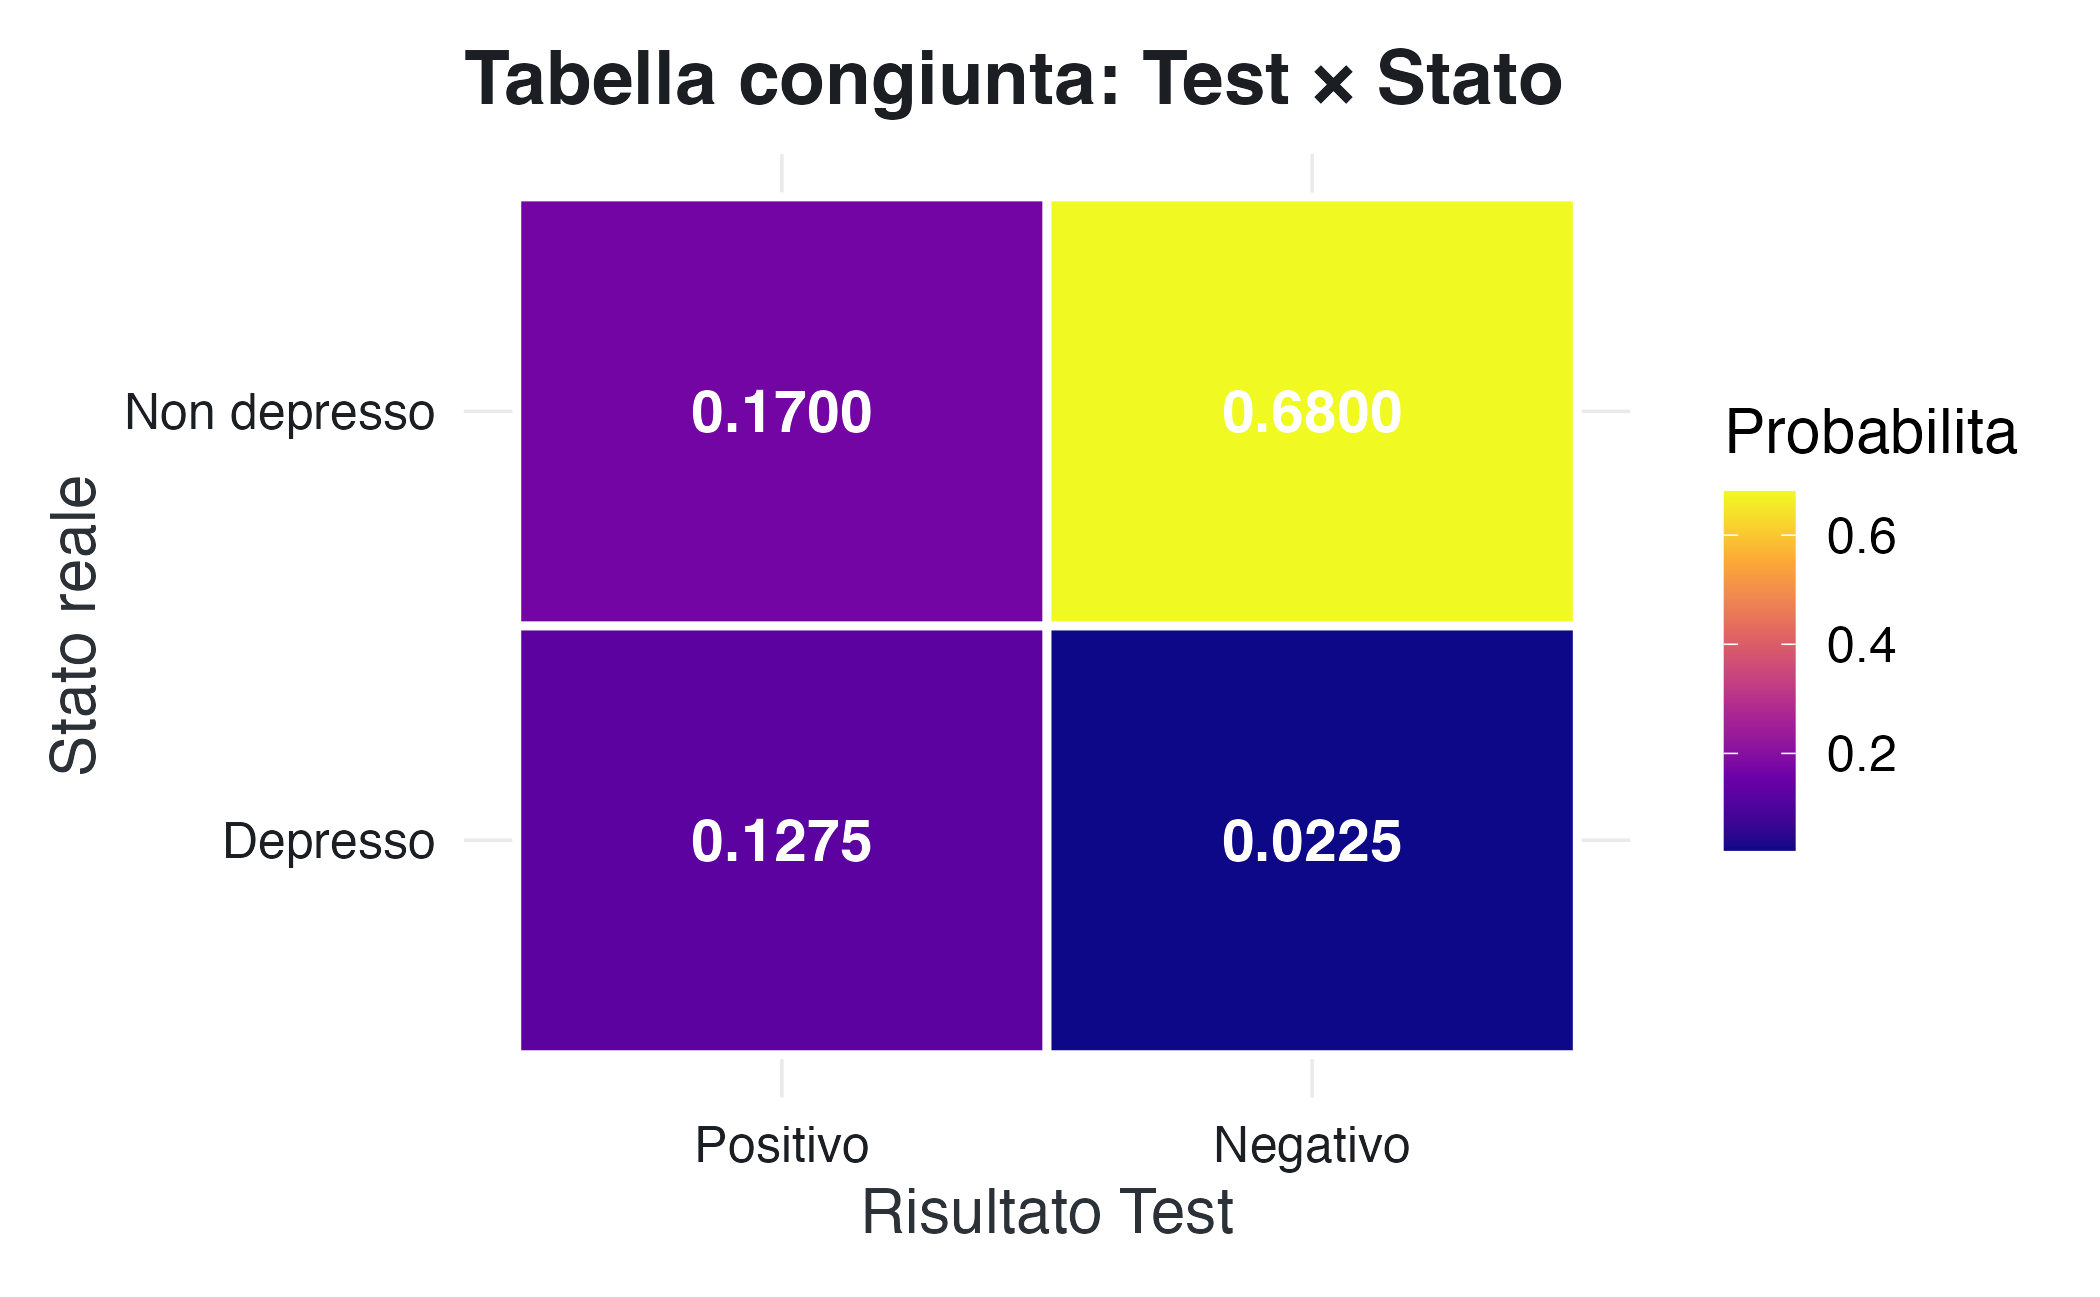
\includegraphics[width=0.85\linewidth,height=\textheight,keepaspectratio]{chapters/probability/02_axioms_coherence_bayesian_files/figure-pdf/unnamed-chunk-4-1.png}

\subsubsection*{Verifica empirica mediante
simulazione}\label{verifica-empirica-mediante-simulazione}

La coerenza della distribuzione congiunta può essere verificata
empiricamente attraverso simulazione:

\begin{Shaded}
\begin{Highlighting}[]
\FunctionTok{set.seed}\NormalTok{(}\DecValTok{123}\NormalTok{)}
\NormalTok{N }\OtherTok{\textless{}{-}} \DecValTok{100000}

\CommentTok{\# Simulare secondo la distribuzione congiunta}
\NormalTok{probs\_vector }\OtherTok{\textless{}{-}} \FunctionTok{c}\NormalTok{(p\_depresso\_positivo, p\_depresso\_negativo, }
\NormalTok{                  p\_non\_depresso\_positivo, p\_non\_depresso\_negativo)}

\NormalTok{outcomes }\OtherTok{\textless{}{-}} \FunctionTok{sample}\NormalTok{(}\DecValTok{1}\SpecialCharTok{:}\DecValTok{4}\NormalTok{, }\AttributeTok{size =}\NormalTok{ N, }\AttributeTok{replace =} \ConstantTok{TRUE}\NormalTok{, }\AttributeTok{prob =}\NormalTok{ probs\_vector)}

\CommentTok{\# Contare frequenze empiriche}
\NormalTok{freq\_empiriche }\OtherTok{\textless{}{-}} \FunctionTok{table}\NormalTok{(outcomes) }\SpecialCharTok{/}\NormalTok{ N}

\CommentTok{\# Confronto tra probabilità teoriche e frequenze empiriche}
\NormalTok{df\_verifica }\OtherTok{\textless{}{-}} \FunctionTok{data.frame}\NormalTok{(}
  \AttributeTok{Configurazione =} \FunctionTok{c}\NormalTok{(}\StringTok{"D∩T+"}\NormalTok{, }\StringTok{"D∩T{-}"}\NormalTok{, }\StringTok{"D\^{}c∩T+"}\NormalTok{, }\StringTok{"D\^{}c∩T{-}"}\NormalTok{),}
  \AttributeTok{Teorica =}\NormalTok{ probs\_vector,}
  \AttributeTok{Empirica =} \FunctionTok{as.numeric}\NormalTok{(freq\_empiriche)}
\NormalTok{)}

\NormalTok{df\_verifica}\SpecialCharTok{$}\NormalTok{Teorica }\OtherTok{\textless{}{-}} \FunctionTok{round}\NormalTok{(df\_verifica}\SpecialCharTok{$}\NormalTok{Teorica, }\DecValTok{4}\NormalTok{)}
\NormalTok{df\_verifica}\SpecialCharTok{$}\NormalTok{Empirica }\OtherTok{\textless{}{-}} \FunctionTok{round}\NormalTok{(df\_verifica}\SpecialCharTok{$}\NormalTok{Empirica, }\DecValTok{4}\NormalTok{)}
\FunctionTok{print}\NormalTok{(df\_verifica)}
\CommentTok{\#\textgreater{}   Configurazione Teorica Empirica}
\CommentTok{\#\textgreater{} 1           D∩T+  0.1275   0.1266}
\CommentTok{\#\textgreater{} 2           D∩T{-}  0.0225   0.0226}
\CommentTok{\#\textgreater{} 3         D\^{}c∩T+  0.1700   0.1699}
\CommentTok{\#\textgreater{} 4         D\^{}c∩T{-}  0.6800   0.6809}
\end{Highlighting}
\end{Shaded}

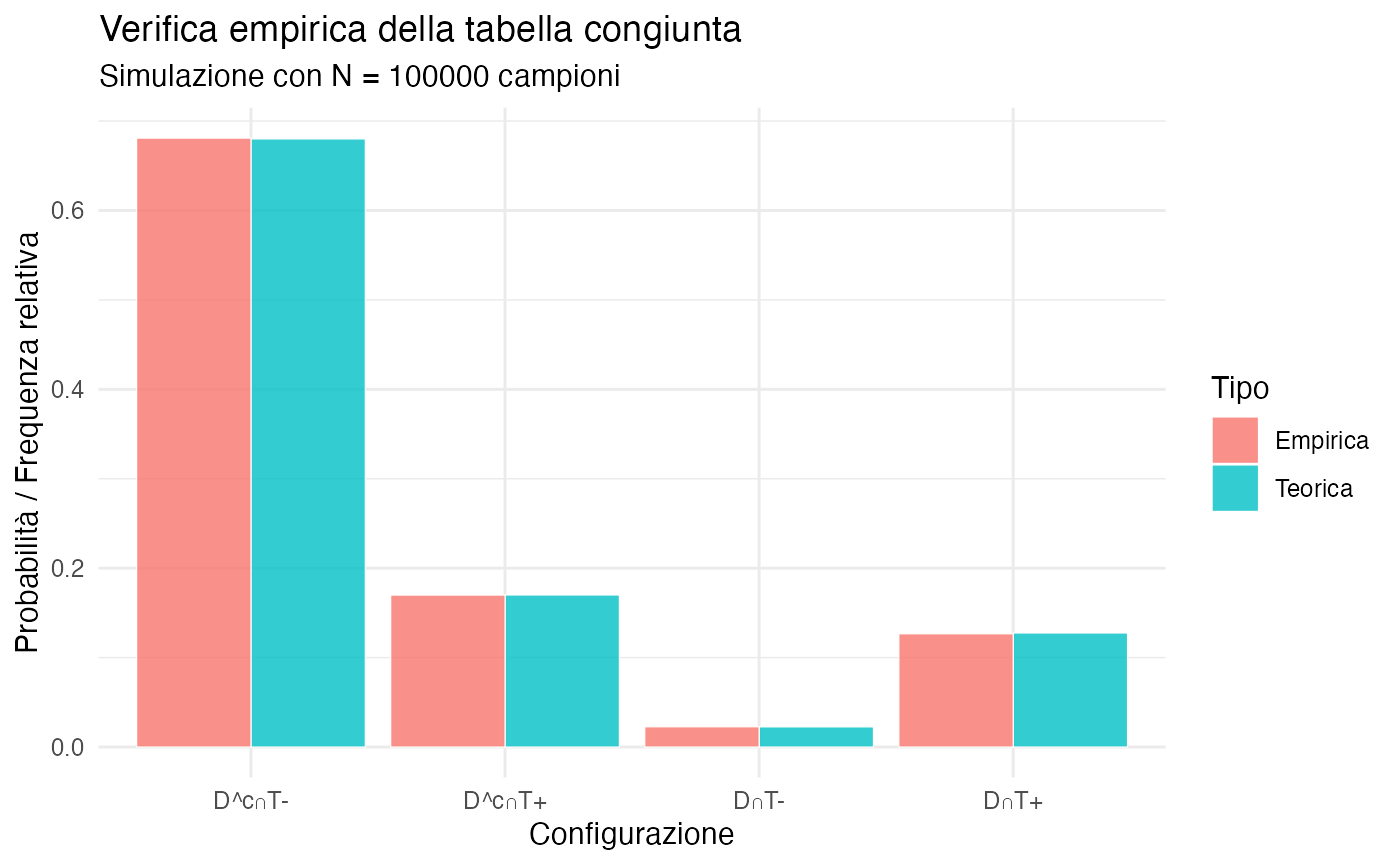
\includegraphics[width=0.85\linewidth,height=\textheight,keepaspectratio]{chapters/probability/02_axioms_coherence_bayesian_files/figure-pdf/unnamed-chunk-6-1.png}

La convergenza delle frequenze empiriche verso le probabilità teoriche
conferma che la tabella di probabilità congiunta rappresenta un sistema
di credenze coerente in grado di generare i dati attesi.

\end{tcolorbox}

\subsection{Calcolo di probabilità marginali e
condizionate}\label{calcolo-di-probabilituxe0-marginali-e-condizionate}

La distribuzione congiunta rappresenta la conoscenza completa del
sistema analizzato e costituisce il fondamento da cui è possibile
dedurre in modo coerente tutte le altre probabilità di interesse.

\subsection{Probabilità marginali}\label{probabilituxe0-marginali}

Le probabilità \emph{marginali} si ottengono mediante sommazione lungo
una dimensione della tabella congiunta. Formalmente:

\[
P(A) = P(A \cap B) + P(A \cap B^c),
\]

\[
P(B) = P(A \cap B) + P(A^c \cap B).
\]

Questo calcolo corrisponde a proiettare la distribuzione congiunta su
ciascuna variabile singolarmente, ignorando l'altra dimensione.

\begin{verbatim}
#> Probabilità marginali derivate:
#> P(D) = 0.15
#> P(D^c) = 0.85
#> P(T+) = 0.297
#> P(T-) = 0.703
\end{verbatim}

\subsection{Probabilità condizionate}\label{probabilituxe0-condizionate}

Le probabilità \emph{condizionate} emergono come rapporto tra
probabilità congiunta e probabilità marginale dell'evento condizionante:

\[
P(A \mid B) = \frac{P(A \cap B)}{P(B)}.
\]

Epistemicamente, esse rappresentano l'aggiornamento delle nostre
credenze una volta acquisita l'informazione che l'evento \(B\) si è
verificato: lo spazio delle possibilità si restringe alle configurazioni
compatibili con \(B\), e le probabilità vengono conseguentemente
rinormalizzate.

\begin{verbatim}
#> Probabilità condizionate derivate:
#> P(D | T+) = 0.429 (Valore predittivo positivo)
#> P(D | T-) = 0.032 (Probabilità residua dopo test negativo)
\end{verbatim}

\begin{tcolorbox}[enhanced jigsaw, arc=.35mm, breakable, colbacktitle=quarto-callout-important-color!10!white, opacityback=0, toprule=.15mm, rightrule=.15mm, colback=white, opacitybacktitle=0.6, leftrule=.75mm, coltitle=black, bottomtitle=1mm, left=2mm, toptitle=1mm, title=\textcolor{quarto-callout-important-color}{\faExclamation}\hspace{0.5em}{Messaggio chiave: la coerenza delle probabilità condizionate}, titlerule=0mm, bottomrule=.15mm, colframe=quarto-callout-important-color-frame]

Le probabilità condizionate non rappresentano assegnazioni indipendenti,
ma derivano necessariamente dalla distribuzione congiunta attraverso
operazioni matematiche ben definite.

Questa dipendenza strutturale garantisce la coerenza interna dell'intero
sistema probabilistico. Qualora si tentasse di specificare probabilità
condizionate in modo arbitrario e indipendente dalla distribuzione
congiunta, si incorrerebbe in serie incoerenze quali:

\begin{itemize}
\tightlist
\item
  discrepanze tra il prodotto \(P(A \mid B) \cdot P(B)\) e la
  probabilità congiunta \(P(A \cap B)\);
\item
  violazioni degli assiomi fondamentali della probabilità;
\item
  esposizione al rischio di un \emph{Dutch book}, situazione in cui una
  combinazione di scommesse condurrebbe a una perdita certa.
\end{itemize}

La distribuzione congiunta funge dunque da fondamento coerente da cui
tutte le altre quantità probabilistiche discendono logicamente.

\end{tcolorbox}

\subsection{Visualizzazione: dalla congiunta alle
condizionate}\label{visualizzazione-dalla-congiunta-alle-condizionate}

\begin{center}
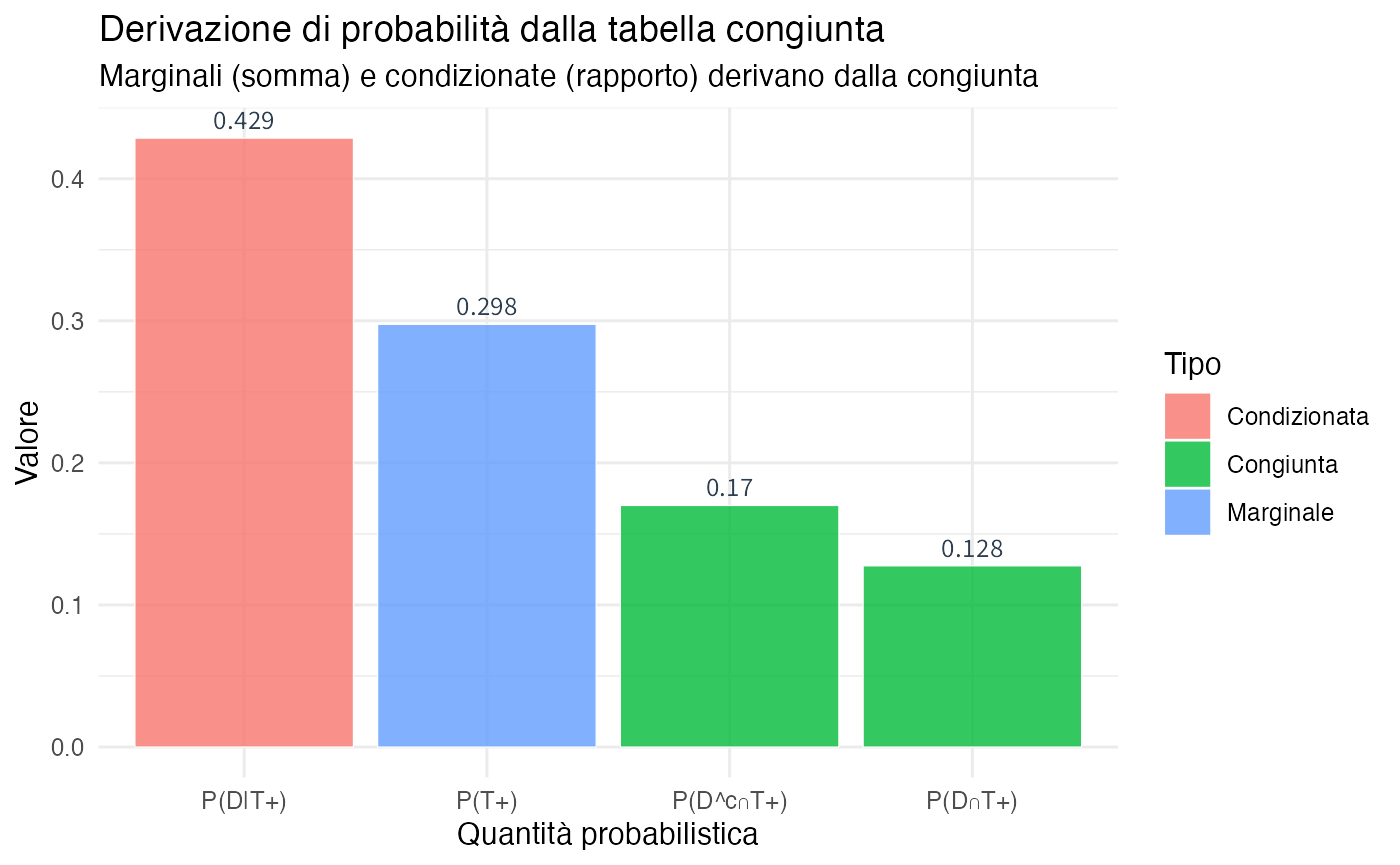
\includegraphics[width=0.85\linewidth,height=\textheight,keepaspectratio]{chapters/probability/02_axioms_coherence_bayesian_files/figure-pdf/unnamed-chunk-9-1.png}
\end{center}

\section{Esercizio guidato: costruire e analizzare una tabella
2×2}\label{esercizio-guidato-costruire-e-analizzare-una-tabella-22}

Lavoriamo attraverso un approccio sistematico per la costruzione di una
tabella di probabilità congiunta a partire da informazioni cliniche.

\begin{tcolorbox}[enhanced jigsaw, arc=.35mm, breakable, colbacktitle=quarto-callout-tip-color!10!white, opacityback=0, toprule=.15mm, rightrule=.15mm, colback=white, opacitybacktitle=0.6, leftrule=.75mm, coltitle=black, bottomtitle=1mm, left=2mm, toptitle=1mm, title=\textcolor{quarto-callout-tip-color}{\faLightbulb}\hspace{0.5em}{Scenario clinico}, titlerule=0mm, bottomrule=.15mm, colframe=quarto-callout-tip-color-frame]

\subsection{Comorbidità Depressione-Ansia in
terapia}\label{comorbidituxe0-depressione-ansia-in-terapia}

Uno psicoterapeuta intende modellare probabilisticamente la comorbidità
nel proprio contesto clinico. Sulla base della letteratura scientifica e
dell'esperienza clinica accumulata, stabilisce i seguenti parametri:

\begin{itemize}
\tightlist
\item
  \(P(\text{Depressione}) = 0.50\) (prevalenza nel setting
  ambulatoriale);
\item
  \(P(\text{Ansia}) = 0.40\);
\item
  \(P(\text{Ansia} \mid \text{Depressione}) = 0.60\) (probabilità di
  comorbidità condizionata).
\end{itemize}

\textbf{Obiettivo}: Costruire la tabella di probabilità congiunta
completa e derivare risposte a specifiche domande cliniche.

\end{tcolorbox}

Parametri:

\begin{Shaded}
\begin{Highlighting}[]
\NormalTok{P\_D }\OtherTok{\textless{}{-}} \FloatTok{0.50}
\NormalTok{P\_A }\OtherTok{\textless{}{-}} \FloatTok{0.40}
\NormalTok{P\_A\_given\_D }\OtherTok{\textless{}{-}} \FloatTok{0.60}
\end{Highlighting}
\end{Shaded}

Passo 1: Calcolare congiunta \(P(D \cap A)\):

\begin{Shaded}
\begin{Highlighting}[]
\NormalTok{P\_D\_and\_A }\OtherTok{\textless{}{-}}\NormalTok{ P\_A\_given\_D }\SpecialCharTok{*}\NormalTok{ P\_D}
\FunctionTok{cat}\NormalTok{(}\StringTok{"Passo 1: P(D ∩ A) = P(A|D) × P(D) ="}\NormalTok{, P\_A\_given\_D, }\StringTok{"×"}\NormalTok{, P\_D, }\StringTok{"="}\NormalTok{, P\_D\_and\_A, }\StringTok{"}\SpecialCharTok{\textbackslash{}n\textbackslash{}n}\StringTok{"}\NormalTok{)}
\CommentTok{\#\textgreater{} Passo 1: P(D ∩ A) = P(A|D) × P(D) = 0.6 × 0.5 = 0.3}
\end{Highlighting}
\end{Shaded}

Passo 2: le altre celle si possono calcolare usando l'additività:

\begin{Shaded}
\begin{Highlighting}[]
\NormalTok{P\_D\_and\_notA }\OtherTok{\textless{}{-}}\NormalTok{ P\_D }\SpecialCharTok{{-}}\NormalTok{ P\_D\_and\_A}
\NormalTok{P\_notD\_and\_A }\OtherTok{\textless{}{-}}\NormalTok{ P\_A }\SpecialCharTok{{-}}\NormalTok{ P\_D\_and\_A}
\NormalTok{P\_notD\_and\_notA }\OtherTok{\textless{}{-}} \DecValTok{1} \SpecialCharTok{{-}}\NormalTok{ (P\_D\_and\_A }\SpecialCharTok{+}\NormalTok{ P\_D\_and\_notA }\SpecialCharTok{+}\NormalTok{ P\_notD\_and\_A)}

\FunctionTok{cat}\NormalTok{(}\StringTok{"Passo 2: Altre celle}\SpecialCharTok{\textbackslash{}n}\StringTok{"}\NormalTok{)}
\CommentTok{\#\textgreater{} Passo 2: Altre celle}
\FunctionTok{cat}\NormalTok{(}\StringTok{"  P(D ∩ A\^{}c) ="}\NormalTok{, P\_D\_and\_notA, }\StringTok{"}\SpecialCharTok{\textbackslash{}n}\StringTok{"}\NormalTok{)}
\CommentTok{\#\textgreater{}   P(D ∩ A\^{}c) = 0.2}
\FunctionTok{cat}\NormalTok{(}\StringTok{"  P(D\^{}c ∩ A) ="}\NormalTok{, P\_notD\_and\_A, }\StringTok{"}\SpecialCharTok{\textbackslash{}n}\StringTok{"}\NormalTok{)}
\CommentTok{\#\textgreater{}   P(D\^{}c ∩ A) = 0.1}
\FunctionTok{cat}\NormalTok{(}\StringTok{"  P(D\^{}c ∩ A\^{}c) ="}\NormalTok{, P\_notD\_and\_notA, }\StringTok{"}\SpecialCharTok{\textbackslash{}n\textbackslash{}n}\StringTok{"}\NormalTok{)}
\CommentTok{\#\textgreater{}   P(D\^{}c ∩ A\^{}c) = 0.4}
\end{Highlighting}
\end{Shaded}

Passo 3: Verificare coerenza:

\begin{Shaded}
\begin{Highlighting}[]
\NormalTok{somma\_celle }\OtherTok{\textless{}{-}}\NormalTok{ P\_D\_and\_A }\SpecialCharTok{+}\NormalTok{ P\_D\_and\_notA }\SpecialCharTok{+}\NormalTok{ P\_notD\_and\_A }\SpecialCharTok{+}\NormalTok{ P\_notD\_and\_notA}
\FunctionTok{cat}\NormalTok{(}\StringTok{"Passo 3: Verifica coerenza}\SpecialCharTok{\textbackslash{}n}\StringTok{"}\NormalTok{)}
\CommentTok{\#\textgreater{} Passo 3: Verifica coerenza}
\FunctionTok{cat}\NormalTok{(}\StringTok{"  Somma celle ="}\NormalTok{, somma\_celle, }\StringTok{"(deve essere 1) ✓}\SpecialCharTok{\textbackslash{}n\textbackslash{}n}\StringTok{"}\NormalTok{)}
\CommentTok{\#\textgreater{}   Somma celle = 1 (deve essere 1) ✓}
\end{Highlighting}
\end{Shaded}

Creare tabella:

\begin{Shaded}
\begin{Highlighting}[]
\NormalTok{tab\_comorbid }\OtherTok{\textless{}{-}} \FunctionTok{matrix}\NormalTok{(}
  \FunctionTok{c}\NormalTok{(P\_D\_and\_A, P\_D\_and\_notA,}
\NormalTok{    P\_notD\_and\_A, P\_notD\_and\_notA),}
  \AttributeTok{nrow =} \DecValTok{2}\NormalTok{, }\AttributeTok{byrow =} \ConstantTok{TRUE}\NormalTok{,}
  \AttributeTok{dimnames =} \FunctionTok{list}\NormalTok{(}
    \AttributeTok{Depressione =} \FunctionTok{c}\NormalTok{(}\StringTok{"D"}\NormalTok{, }\StringTok{"D\^{}c"}\NormalTok{),}
    \AttributeTok{Ansia =} \FunctionTok{c}\NormalTok{(}\StringTok{"A"}\NormalTok{, }\StringTok{"A\^{}c"}\NormalTok{)}
\NormalTok{  )}
\NormalTok{)}

\FunctionTok{cat}\NormalTok{(}\StringTok{"TABELLA CONGIUNTA FINALE:}\SpecialCharTok{\textbackslash{}n}\StringTok{"}\NormalTok{)}
\CommentTok{\#\textgreater{} TABELLA CONGIUNTA FINALE:}
\FunctionTok{print}\NormalTok{(}\FunctionTok{round}\NormalTok{(tab\_comorbid, }\DecValTok{3}\NormalTok{))}
\CommentTok{\#\textgreater{}            Ansia}
\CommentTok{\#\textgreater{} Depressione   A A\^{}c}
\CommentTok{\#\textgreater{}         D   0.3 0.2}
\CommentTok{\#\textgreater{}         D\^{}c 0.1 0.4}
\end{Highlighting}
\end{Shaded}

\begin{Shaded}
\begin{Highlighting}[]
\FunctionTok{cat}\NormalTok{(}\StringTok{"}\SpecialCharTok{\textbackslash{}n}\StringTok{MARGINALI:}\SpecialCharTok{\textbackslash{}n}\StringTok{"}\NormalTok{)}
\CommentTok{\#\textgreater{} }
\CommentTok{\#\textgreater{} MARGINALI:}
\FunctionTok{cat}\NormalTok{(}\StringTok{"Riga (Depressione):"}\NormalTok{, }\FunctionTok{round}\NormalTok{(}\FunctionTok{rowSums}\NormalTok{(tab\_comorbid), }\DecValTok{3}\NormalTok{), }\StringTok{"}\SpecialCharTok{\textbackslash{}n}\StringTok{"}\NormalTok{)}
\CommentTok{\#\textgreater{} Riga (Depressione): 0.5 0.5}
\FunctionTok{cat}\NormalTok{(}\StringTok{"Colonna (Ansia):"}\NormalTok{, }\FunctionTok{round}\NormalTok{(}\FunctionTok{colSums}\NormalTok{(tab\_comorbid), }\DecValTok{3}\NormalTok{), }\StringTok{"}\SpecialCharTok{\textbackslash{}n}\StringTok{"}\NormalTok{)}
\CommentTok{\#\textgreater{} Colonna (Ansia): 0.4 0.6}
\end{Highlighting}
\end{Shaded}

\subsection{Risposte a domande
cliniche}\label{risposte-a-domande-cliniche}

Q1: Probabilità di almeno una condizione:

\begin{Shaded}
\begin{Highlighting}[]
\NormalTok{P\_D\_or\_A }\OtherTok{\textless{}{-}}\NormalTok{ P\_D }\SpecialCharTok{+}\NormalTok{ P\_A }\SpecialCharTok{{-}}\NormalTok{ P\_D\_and\_A}
\FunctionTok{cat}\NormalTok{(}\StringTok{"Q1: P(D ∪ A) = P(almeno una condizione) ="}\NormalTok{, }\FunctionTok{round}\NormalTok{(P\_D\_or\_A, }\DecValTok{3}\NormalTok{), }\StringTok{"}\SpecialCharTok{\textbackslash{}n}\StringTok{"}\NormalTok{)}
\CommentTok{\#\textgreater{} Q1: P(D ∪ A) = P(almeno una condizione) = 0.6}
\end{Highlighting}
\end{Shaded}

Q2: Probabilità di nessuna condizione:

\begin{Shaded}
\begin{Highlighting}[]
\NormalTok{P\_neither }\OtherTok{\textless{}{-}}\NormalTok{ P\_notD\_and\_notA}
\FunctionTok{cat}\NormalTok{(}\StringTok{"Q2: P(D\^{}c ∩ A\^{}c) = P(nessuna condizione) ="}\NormalTok{, }\FunctionTok{round}\NormalTok{(P\_neither, }\DecValTok{3}\NormalTok{), }\StringTok{"}\SpecialCharTok{\textbackslash{}n}\StringTok{"}\NormalTok{)}
\CommentTok{\#\textgreater{} Q2: P(D\^{}c ∩ A\^{}c) = P(nessuna condizione) = 0.4}
\end{Highlighting}
\end{Shaded}

Q3: Probabilità di comorbidità:

\begin{Shaded}
\begin{Highlighting}[]
\FunctionTok{cat}\NormalTok{(}\StringTok{"Q3: P(D ∩ A) = P(entrambe le condizioni) ="}\NormalTok{, }\FunctionTok{round}\NormalTok{(P\_D\_and\_A, }\DecValTok{3}\NormalTok{), }\StringTok{"}\SpecialCharTok{\textbackslash{}n}\StringTok{"}\NormalTok{)}
\CommentTok{\#\textgreater{} Q3: P(D ∩ A) = P(entrambe le condizioni) = 0.3}
\end{Highlighting}
\end{Shaded}

Q4: \(P(D \mid A)\) -- Se un paziente manifesta un disturbo d'ansia,
qual è la probabilità che sia anche depresso?

\begin{Shaded}
\begin{Highlighting}[]
\NormalTok{P\_D\_given\_A }\OtherTok{\textless{}{-}}\NormalTok{ P\_D\_and\_A }\SpecialCharTok{/}\NormalTok{ P\_A}
\FunctionTok{cat}\NormalTok{(}\StringTok{"Q4: P(D | A) = P(Depressione dato Ansia) ="}\NormalTok{, }\FunctionTok{round}\NormalTok{(P\_D\_given\_A, }\DecValTok{3}\NormalTok{), }\StringTok{"}\SpecialCharTok{\textbackslash{}n}\StringTok{"}\NormalTok{)}
\CommentTok{\#\textgreater{} Q4: P(D | A) = P(Depressione dato Ansia) = 0.75}
\end{Highlighting}
\end{Shaded}

Q5: Le condizioni sono indipendenti?

\begin{Shaded}
\begin{Highlighting}[]
\CommentTok{\# Test: P(D ∩ A) =? P(D) × P(A)}
\NormalTok{P\_D\_times\_P\_A }\OtherTok{\textless{}{-}}\NormalTok{ P\_D }\SpecialCharTok{*}\NormalTok{ P\_A}
\FunctionTok{cat}\NormalTok{(}\StringTok{"}\SpecialCharTok{\textbackslash{}n}\StringTok{Q5: Test di indipendenza}\SpecialCharTok{\textbackslash{}n}\StringTok{"}\NormalTok{)}
\CommentTok{\#\textgreater{} }
\CommentTok{\#\textgreater{} Q5: Test di indipendenza}
\FunctionTok{cat}\NormalTok{(}\StringTok{"  P(D) × P(A) ="}\NormalTok{, }\FunctionTok{round}\NormalTok{(P\_D\_times\_P\_A, }\DecValTok{3}\NormalTok{), }\StringTok{"}\SpecialCharTok{\textbackslash{}n}\StringTok{"}\NormalTok{)}
\CommentTok{\#\textgreater{}   P(D) × P(A) = 0.2}
\FunctionTok{cat}\NormalTok{(}\StringTok{"  P(D ∩ A) ="}\NormalTok{, }\FunctionTok{round}\NormalTok{(P\_D\_and\_A, }\DecValTok{3}\NormalTok{), }\StringTok{"}\SpecialCharTok{\textbackslash{}n}\StringTok{"}\NormalTok{)}
\CommentTok{\#\textgreater{}   P(D ∩ A) = 0.3}
\ControlFlowTok{if}\NormalTok{ (}\FunctionTok{abs}\NormalTok{(P\_D\_and\_A }\SpecialCharTok{{-}}\NormalTok{ P\_D\_times\_P\_A) }\SpecialCharTok{\textless{}} \FloatTok{1e{-}9}\NormalTok{) \{}
  \FunctionTok{cat}\NormalTok{(}\StringTok{"  → Eventi INDIPENDENTI}\SpecialCharTok{\textbackslash{}n}\StringTok{"}\NormalTok{)}
\NormalTok{\} }\ControlFlowTok{else}\NormalTok{ \{}
  \FunctionTok{cat}\NormalTok{(}\StringTok{"  → Eventi DIPENDENTI (correlati)}\SpecialCharTok{\textbackslash{}n}\StringTok{"}\NormalTok{)}
  \FunctionTok{cat}\NormalTok{(}\StringTok{"  Differenza:"}\NormalTok{, }\FunctionTok{round}\NormalTok{(P\_D\_and\_A }\SpecialCharTok{{-}}\NormalTok{ P\_D\_times\_P\_A, }\DecValTok{3}\NormalTok{), }\StringTok{"}\SpecialCharTok{\textbackslash{}n}\StringTok{"}\NormalTok{)}
\NormalTok{\}}
\CommentTok{\#\textgreater{}   → Eventi DIPENDENTI (correlati)}
\CommentTok{\#\textgreater{}   Differenza: 0.1}
\end{Highlighting}
\end{Shaded}

\subsection{Visualizzazione della tabella
congiunta}\label{visualizzazione-della-tabella-congiunta-1}

\begin{Shaded}
\begin{Highlighting}[]
\CommentTok{\# Heatmap}
\NormalTok{df\_comorbid }\OtherTok{\textless{}{-}} \FunctionTok{as.data.frame}\NormalTok{(}\FunctionTok{as.table}\NormalTok{(tab\_comorbid))}
\FunctionTok{colnames}\NormalTok{(df\_comorbid) }\OtherTok{\textless{}{-}} \FunctionTok{c}\NormalTok{(}\StringTok{"Depressione"}\NormalTok{, }\StringTok{"Ansia"}\NormalTok{, }\StringTok{"Probabilita"}\NormalTok{)}

\FunctionTok{ggplot}\NormalTok{(df\_comorbid, }\FunctionTok{aes}\NormalTok{(}\AttributeTok{x =}\NormalTok{ Ansia, }\AttributeTok{y =}\NormalTok{ Depressione, }\AttributeTok{fill =}\NormalTok{ Probabilita)) }\SpecialCharTok{+}
  \FunctionTok{geom\_tile}\NormalTok{(}\AttributeTok{color =} \StringTok{"white"}\NormalTok{, }\AttributeTok{size =} \DecValTok{2}\NormalTok{) }\SpecialCharTok{+}
  \FunctionTok{geom\_text}\NormalTok{(}\FunctionTok{aes}\NormalTok{(}\AttributeTok{label =} \FunctionTok{round}\NormalTok{(Probabilita, }\DecValTok{3}\NormalTok{)), }
            \AttributeTok{color =} \StringTok{"white"}\NormalTok{, }\AttributeTok{size =} \DecValTok{8}\NormalTok{, }\AttributeTok{fontface =} \StringTok{"bold"}\NormalTok{) }\SpecialCharTok{+}
  \FunctionTok{scale\_fill\_viridis\_c}\NormalTok{(}\AttributeTok{option =} \StringTok{"plasma"}\NormalTok{) }\SpecialCharTok{+}
  \FunctionTok{labs}\NormalTok{(}
    \AttributeTok{title =} \StringTok{"Tabella congiunta: Depressione × Ansia"}\NormalTok{,}
    \AttributeTok{subtitle =} \StringTok{"Comorbidità P(D ∩ A) = 0.30 (cella in alto a sinistra)"}
\NormalTok{  ) }\SpecialCharTok{+}
  \FunctionTok{theme\_minimal}\NormalTok{() }\SpecialCharTok{+}
  \FunctionTok{coord\_fixed}\NormalTok{()}
\end{Highlighting}
\end{Shaded}

\begin{center}
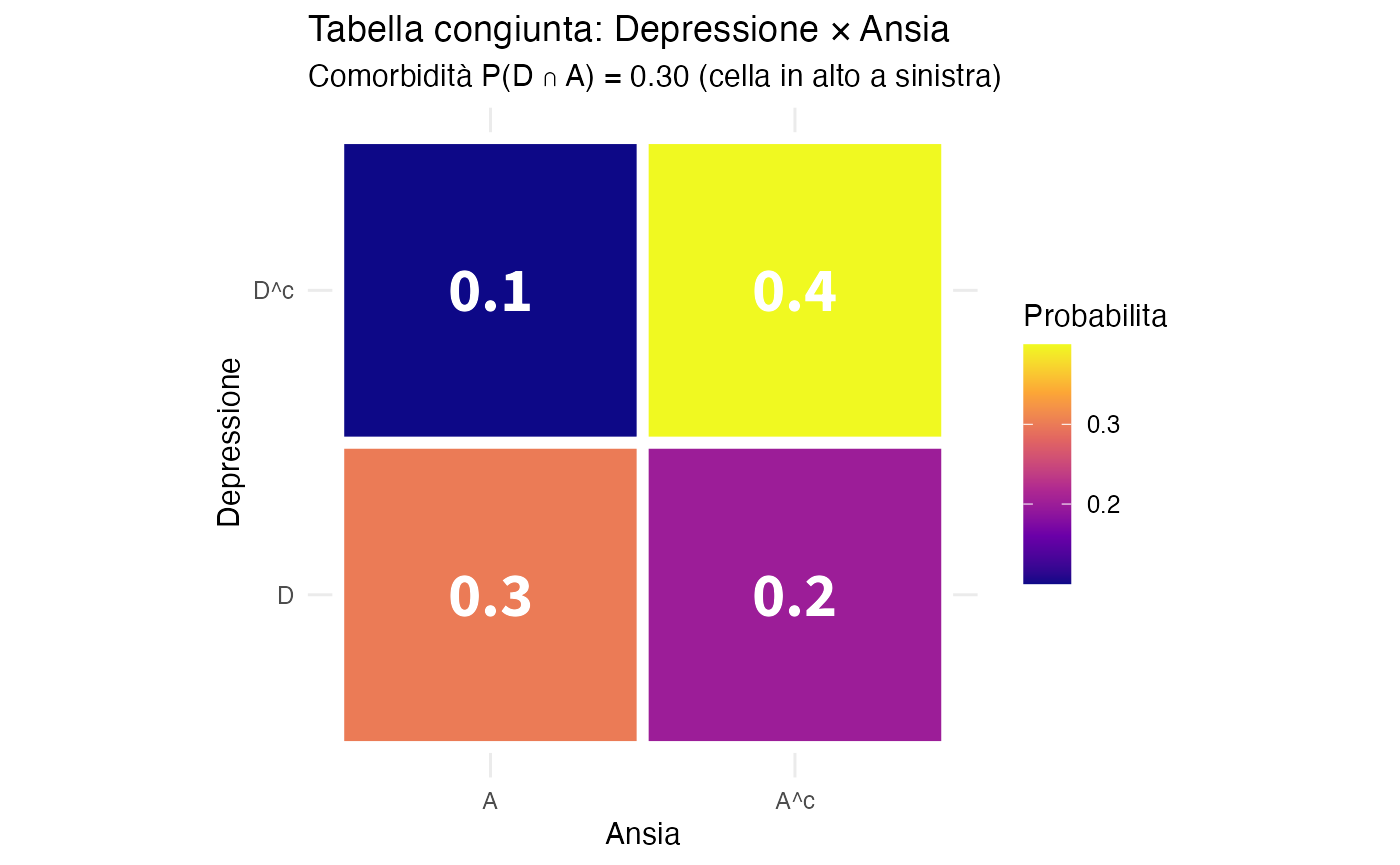
\includegraphics[width=0.85\linewidth,height=\textheight,keepaspectratio]{chapters/probability/02_axioms_coherence_bayesian_files/figure-pdf/unnamed-chunk-21-1.png}
\end{center}

\section{Estensione a tabelle
multidimensionali}\label{estensione-a-tabelle-multidimensionali}

Il principio della distribuzione congiunta si generalizza naturalmente a
sistemi caratterizzati da molteplici variabili e categorie, consentendo
la modellazione di scenari clinici di maggiore complessità.

\subsection{Esempio: depressione e livelli di
ansia}\label{esempio-depressione-e-livelli-di-ansia}

Consideriamo uno scenario clinico che coinvolge due dimensioni distinte:

\begin{itemize}
\tightlist
\item
  depressione: presenza/assenza (variabile dicotomica);
\item
  severità dell'ansia: nessuna/lieve/grave (variabile a tre livelli).
\end{itemize}

\begin{Shaded}
\begin{Highlighting}[]
\CommentTok{\# Scenario: Depressione × Severità Ansia (Nessuna/Lieve/Grave)}
\NormalTok{tab\_2x3 }\OtherTok{\textless{}{-}} \FunctionTok{matrix}\NormalTok{(}
  \FunctionTok{c}\NormalTok{(}\FloatTok{0.15}\NormalTok{, }\FloatTok{0.20}\NormalTok{, }\FloatTok{0.15}\NormalTok{,  }\CommentTok{\# D: Ansia Nessuna/Lieve/Grave}
    \FloatTok{0.35}\NormalTok{, }\FloatTok{0.10}\NormalTok{, }\FloatTok{0.05}\NormalTok{), }\CommentTok{\# D\^{}c: Ansia Nessuna/Lieve/Grave}
  \AttributeTok{nrow =} \DecValTok{2}\NormalTok{, }\AttributeTok{byrow =} \ConstantTok{TRUE}\NormalTok{,}
  \AttributeTok{dimnames =} \FunctionTok{list}\NormalTok{(}
    \AttributeTok{Depressione =} \FunctionTok{c}\NormalTok{(}\StringTok{"D"}\NormalTok{, }\StringTok{"D\^{}c"}\NormalTok{),}
    \AttributeTok{Ansia =} \FunctionTok{c}\NormalTok{(}\StringTok{"Nessuna"}\NormalTok{, }\StringTok{"Lieve"}\NormalTok{, }\StringTok{"Grave"}\NormalTok{)}
\NormalTok{  )}
\NormalTok{)}

\FunctionTok{cat}\NormalTok{(}\StringTok{"Tabella 2×3:}\SpecialCharTok{\textbackslash{}n}\StringTok{"}\NormalTok{)}
\CommentTok{\#\textgreater{} Tabella 2×3:}
\FunctionTok{print}\NormalTok{(tab\_2x3)}
\CommentTok{\#\textgreater{}            Ansia}
\CommentTok{\#\textgreater{} Depressione Nessuna Lieve Grave}
\CommentTok{\#\textgreater{}         D      0.15   0.2  0.15}
\CommentTok{\#\textgreater{}         D\^{}c    0.35   0.1  0.05}
\end{Highlighting}
\end{Shaded}

\begin{Shaded}
\begin{Highlighting}[]
\FunctionTok{cat}\NormalTok{(}\StringTok{"}\SpecialCharTok{\textbackslash{}n}\StringTok{Marginali:}\SpecialCharTok{\textbackslash{}n}\StringTok{"}\NormalTok{)}
\CommentTok{\#\textgreater{} }
\CommentTok{\#\textgreater{} Marginali:}
\FunctionTok{cat}\NormalTok{(}\StringTok{"Depressione:"}\NormalTok{, }\FunctionTok{rowSums}\NormalTok{(tab\_2x3), }\StringTok{"}\SpecialCharTok{\textbackslash{}n}\StringTok{"}\NormalTok{)}
\CommentTok{\#\textgreater{} Depressione: 0.5 0.5}
\FunctionTok{cat}\NormalTok{(}\StringTok{"Ansia:"}\NormalTok{, }\FunctionTok{colSums}\NormalTok{(tab\_2x3), }\StringTok{"}\SpecialCharTok{\textbackslash{}n}\StringTok{"}\NormalTok{)}
\CommentTok{\#\textgreater{} Ansia: 0.5 0.3 0.2}
\FunctionTok{cat}\NormalTok{(}\StringTok{"Totale:"}\NormalTok{, }\FunctionTok{sum}\NormalTok{(tab\_2x3), }\StringTok{"}\SpecialCharTok{\textbackslash{}n}\StringTok{"}\NormalTok{)}
\CommentTok{\#\textgreater{} Totale: 1}
\end{Highlighting}
\end{Shaded}

\subsection{Visualizzazione della distribuzione
congiunta}\label{visualizzazione-della-distribuzione-congiunta}

\begin{Shaded}
\begin{Highlighting}[]
\NormalTok{df\_2x3 }\OtherTok{\textless{}{-}} \FunctionTok{as.data.frame}\NormalTok{(}\FunctionTok{as.table}\NormalTok{(tab\_2x3))}
\FunctionTok{colnames}\NormalTok{(df\_2x3) }\OtherTok{\textless{}{-}} \FunctionTok{c}\NormalTok{(}\StringTok{"Depressione"}\NormalTok{, }\StringTok{"SeveritaAnsia"}\NormalTok{, }\StringTok{"Probabilita"}\NormalTok{)}

\FunctionTok{ggplot}\NormalTok{(df\_2x3, }\FunctionTok{aes}\NormalTok{(}\AttributeTok{x =}\NormalTok{ SeveritaAnsia, }\AttributeTok{y =}\NormalTok{ Depressione, }\AttributeTok{fill =}\NormalTok{ Probabilita)) }\SpecialCharTok{+}
  \FunctionTok{geom\_tile}\NormalTok{(}\AttributeTok{color =} \StringTok{"white"}\NormalTok{, }\AttributeTok{size =} \DecValTok{1}\NormalTok{) }\SpecialCharTok{+}
  \FunctionTok{geom\_text}\NormalTok{(}\FunctionTok{aes}\NormalTok{(}\AttributeTok{label =} \FunctionTok{round}\NormalTok{(Probabilita, }\DecValTok{2}\NormalTok{)), }
            \AttributeTok{color =} \StringTok{"white"}\NormalTok{, }\AttributeTok{size =} \DecValTok{6}\NormalTok{, }\AttributeTok{fontface =} \StringTok{"bold"}\NormalTok{) }\SpecialCharTok{+}
  \FunctionTok{scale\_fill\_viridis\_c}\NormalTok{(}\AttributeTok{option =} \StringTok{"plasma"}\NormalTok{) }\SpecialCharTok{+}
  \FunctionTok{labs}\NormalTok{(}
    \AttributeTok{title =} \StringTok{"Tabella congiunta 2×3: Depressione × Severità Ansia"}\NormalTok{,}
    \AttributeTok{x =} \StringTok{"Ansia"}\NormalTok{,}
    \AttributeTok{subtitle =} \StringTok{"Ogni cella rappresenta la credenza in una specifica configurazione clinica"}
\NormalTok{  ) }\SpecialCharTok{+}
  \FunctionTok{theme\_minimal}\NormalTok{()}
\end{Highlighting}
\end{Shaded}

\begin{center}
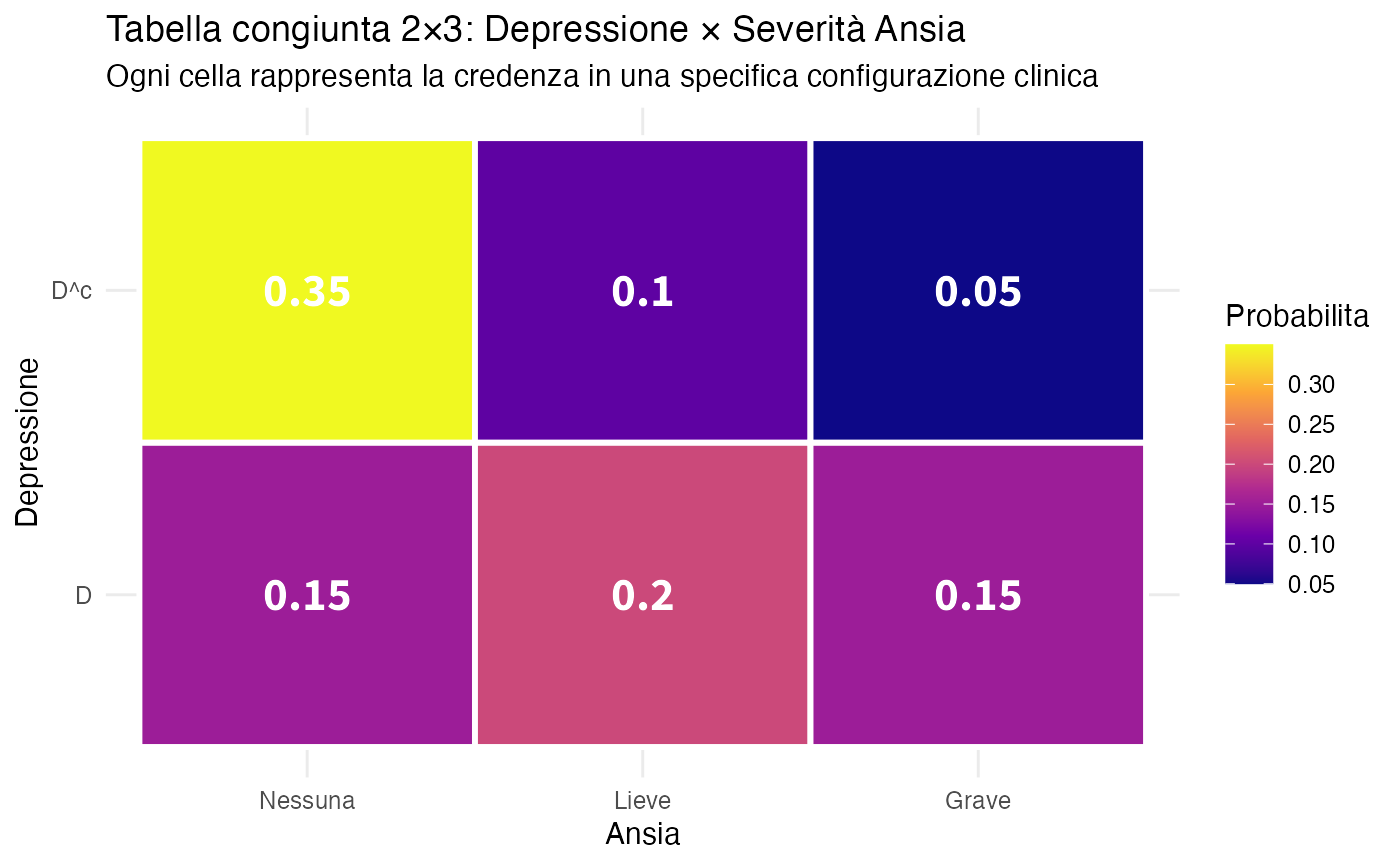
\includegraphics[width=0.85\linewidth,height=\textheight,keepaspectratio]{chapters/probability/02_axioms_coherence_bayesian_files/figure-pdf/unnamed-chunk-24-1.png}
\end{center}

\textbf{Interpretazione clinica:} la distribuzione congiunta rivela i
pattern della presentazione clinica: il 15\% dei pazienti presenta una
comorbilità di depressione con ansia grave, mentre il 20\% mostra una
depressione associata a un'ansia lieve. Una porzione consistente del
35\% comprende pazienti non depressi, senza sintomi d'ansia. Le
probabilità marginali, ottenute sommando i valori lungo le rispettive
dimensioni, forniscono una stima della prevalenza complessiva di
ciascuna condizione nella popolazione clinica di riferimento.

\section*{Riflessioni conclusive}\label{riflessioni-conclusive-1}

\markright{Riflessioni conclusive}

In questo capitolo abbiamo gettato le basi matematiche per esprimere e
manipolare le nostre credenze in modo coerente. Lo spazio campionario è
stato ridefinito in chiave epistemologica: non è l'insieme di tutto ciò
che può accadere fisicamente, ma l'insieme di ciò che riteniamo
possibile, in base al nostro attuale stato di conoscenza.

Gli assiomi della probabilità non emergono come leggi naturali, ma come
condizioni necessarie per garantire la coerenza logica e proteggere da
situazioni di svantaggio certo, come dimostrato dall'argomento del Dutch
Book. I vincoli di Fréchet dimostrano che le probabilità congiunte non
possono essere assegnate arbitrariamente, ma devono rispettare precise
relazioni matematiche con le probabilità marginali.

La distribuzione congiunta si rivela la rappresentazione più completa e
operativa del nostro stato di credenza. Da questa matrice fondamentale
derivano sistematicamente le probabilità marginali mediante la somma
lungo righe o colonne, le probabilità condizionate come rapporti tra
celle, le verifiche di indipendenza mediante il confronto tra prodotti e
probabilità congiunte e qualsiasi altra quantità probabilistica di
interesse.

Le verifiche empiriche mediante simulazione confermano che le credenze
coerenti generano pattern di dati attesi, ribadendo il principio
fondamentale secondo cui i dati non definiscono le credenze, ma
piuttosto le credenze esprimono il nostro stato di incertezza prima
dell'osservazione dei dati.

Questo approccio basato sulle distribuzioni congiunte offre vantaggi
concreti sia alla ricerca che alla pratica psicologica. La trasparenza
garantisce che tutte le assunzioni probabilistiche siano esplicite e
verificabili, mentre il potere diagnostico consente di individuare e
correggere immediatamente le incoerenze logiche. La flessibilità
operativa consente di incorporare agevolmente nuove informazioni
aggiornando la distribuzione, mentre la chiarezza comunicativa rende le
tabelle intuitive e accessibili anche per chi non possiede competenze
statistiche avanzate.

Questo capitolo non solo ha stabilito le modalità di calcolo delle
probabilità, ma ha anche chiarito le ragioni per cui determinate regole
sono necessarie per pensare in modo razionale in condizioni di
incertezza, fornendo le basi concettuali per sviluppare un approccio
bayesiano coerente alla ricerca psicologica.

Nei prossimi capitoli, utilizzeremo questo solido framework per
esplorare l'equiprobabilità come caso speciale di simmetria epistemica,
approfondire l'aggiornamento bayesiano attraverso il calcolo delle
probabilità condizionate e applicare questi strumenti a scenari
psicologici sempre più complessi.

\section*{Esercizi}\label{esercizi}

\markright{Esercizi}

\begin{tcolorbox}[enhanced jigsaw, arc=.35mm, breakable, colbacktitle=quarto-callout-important-color!10!white, opacityback=0, toprule=.15mm, rightrule=.15mm, colback=white, opacitybacktitle=0.6, leftrule=.75mm, coltitle=black, bottomtitle=1mm, left=2mm, toptitle=1mm, title=\textcolor{quarto-callout-important-color}{\faExclamation}\hspace{0.5em}{Problemi}, titlerule=0mm, bottomrule=.15mm, colframe=quarto-callout-important-color-frame]

\subsection{Esercizi sulla coerenza}\label{esercizi-sulla-coerenza}

\begin{enumerate}
\def\labelenumi{\arabic{enumi}.}
\item
  Verifica se le seguenti assegnazioni per eventi mutuamente esclusivi
  sono coerenti:

  \begin{enumerate}
  \def\labelenumii{\alph{enumii}.}
  \tightlist
  \item
    \(P(A) = 0.3, P(B) = 0.4, P(C) = 0.3\)
  \item
    \(P(A) = 0.5, P(B) = 0.4, P(C) = 0.2\)
  \item
    \(P(A) = 0.25, P(B) = 0.25, P(C) = 0.25, P(D) = 0.25\)
  \end{enumerate}
\item
  Un ricercatore assegna \(P(A) = 0.7\) e \(P(A^c) = 0.4\). Identifica
  l'incoerenza e spiega perché viola gli assiomi.
\item
  Per eventi disgiunti \(A\) e \(B\) con \(P(A) = 0.6\) e
  \(P(B) = 0.3\), qualcuno afferma \(P(A \cup B) = 0.8\). È coerente? Se
  no, qual è il valore corretto?
\end{enumerate}

\subsection{Esercizi sui vincoli di
Fréchet}\label{esercizi-sui-vincoli-di-fruxe9chet}

\begin{enumerate}
\def\labelenumi{\arabic{enumi}.}
\setcounter{enumi}{3}
\item
  Dati \(P(A) = 0.4\) e \(P(B) = 0.7\):

  \begin{enumerate}
  \def\labelenumii{\alph{enumii}.}
  \tightlist
  \item
    Calcola i vincoli di Fréchet per \(P(A \cap B)\)
  \item
    Quali dei seguenti valori sono coerenti: 0.05, 0.1, 0.3, 0.5?
  \item
    Visualizza graficamente la regione ammissibile
  \end{enumerate}
\item
  In uno studio su depressione e insonnia:

  \begin{itemize}
  \tightlist
  \item
    \(P(\text{Depressione}) = 0.30\)
  \item
    \(P(\text{Insonnia}) = 0.45\)
  \end{itemize}

  Determina l'intervallo di valori plausibili per
  \(P(\text{Depressione} \cap \text{Insonnia})\).
\item
  Scrivi una funzione R che, dati \(P(A)\) e \(P(B)\), verifichi se un
  proposto \(P(A \cap B)\) rispetta i vincoli di Fréchet.
\end{enumerate}

\subsection{Esercizi su tabelle
congiunte}\label{esercizi-su-tabelle-congiunte}

\begin{enumerate}
\def\labelenumi{\arabic{enumi}.}
\setcounter{enumi}{6}
\item
  Completa la seguente tabella congiunta (alcune celle sono mancanti):

  \begin{longtable}[]{@{}llll@{}}
  \toprule\noalign{}
  & \(B\) & \(B^c\) & Marg. \\
  \midrule\noalign{}
  \endhead
  \bottomrule\noalign{}
  \endlastfoot
  \(A\) & 0.25 & ? & 0.40 \\
  \(A^c\) & ? & 0.45 & ? \\
  Marg. & ? & ? & 1 \\
  \end{longtable}
\item
  Costruisci una tabella congiunta 2×2 per:

  \begin{itemize}
  \tightlist
  \item
    Test COVID: \(P(+) = 0.08\)
  \item
    Malattia: \(P(\text{COVID}) = 0.05\)
  \item
    Sensibilità: \(P(+ \mid \text{COVID}) = 0.90\)
  \end{itemize}

  Calcola poi:

  \begin{enumerate}
  \def\labelenumii{\alph{enumii}.}
  \tightlist
  \item
    \(P(\text{COVID} \mid +)\) (valore predittivo positivo)
  \item
    \(P(\text{COVID} \mid -)\) (probabilità dopo test negativo)
  \item
    Specificità del test
  \end{enumerate}
\item
  Verifica con simulazione Monte Carlo (N=100,000) che la tabella
  dell'esercizio 8 è coerente confrontando frequenze empiriche con
  probabilità teoriche.
\end{enumerate}

\subsection{Esercizi applicati
(psicologia)}\label{esercizi-applicati-psicologia}

\begin{enumerate}
\def\labelenumi{\arabic{enumi}.}
\setcounter{enumi}{9}
\item
  \textbf{Comorbidità}: In un campione clinico:

  \begin{itemize}
  \tightlist
  \item
    \(P(\text{Depressione}) = 0.55\)
  \item
    \(P(\text{PTSD}) = 0.30\)
  \item
    \(P(\text{PTSD} \mid \text{Depressione}) = 0.45\)
  \end{itemize}

  \begin{enumerate}
  \def\labelenumii{\alph{enumii}.}
  \tightlist
  \item
    Costruisci la tabella congiunta completa
  \item
    Calcola \(P(\text{Depressione} \mid \text{PTSD})\)
  \item
    Le due condizioni sono indipendenti?
  \item
    Qual è la probabilità di avere almeno una delle due condizioni?
  \end{enumerate}
\item
  \textbf{Test psicometrico}: Un test di ansia ha:

  \begin{itemize}
  \tightlist
  \item
    Sensibilità: 0.80
  \item
    Specificità: 0.85
  \item
    Prevalenza nell'ambulatorio: 0.25
  \end{itemize}

  \begin{enumerate}
  \def\labelenumii{\alph{enumii}.}
  \tightlist
  \item
    Costruisci la tabella 2×2 per (Ansia × Test)
  \item
    Un paziente ha test positivo. Quanto è probabile che sia ansioso?
  \item
    Se il test è negativo, quanto è probabile l'assenza di ansia?
  \end{enumerate}
\item
  \textbf{Tre diagnosi}: Un paziente può avere Depressione (D), Ansia
  (A), o Nessuna condizione (N). Assegnazioni:

  \begin{itemize}
  \tightlist
  \item
    \(P(D) = 0.40\)
  \item
    \(P(A) = 0.35\)
  \item
    \(P(N) = 0.30\)
  \end{itemize}

  Identifica e correggi l'incoerenza.
\end{enumerate}

\subsection{Esercizi di pensiero
critico}\label{esercizi-di-pensiero-critico}

\begin{enumerate}
\def\labelenumi{\arabic{enumi}.}
\setcounter{enumi}{12}
\item
  Spiega perché, nell'approccio bayesiano, specificare una tabella
  congiunta coerente è ``più fondamentale'' che specificare
  separatamente marginali e condizionate.
\item
  Un frequentista obietta: ``Le tabelle congiunte funzionano solo per
  spazi finiti. Come gestite il caso continuo?'' Rispondi dall'ottica
  bayesiana.
\item
  Due clinici costruiscono tabelle congiunte diverse per Depressione ×
  Test, partendo da prior diversi ma usando la stessa
  sensibilità/specificità. È un problema? Cosa succederebbe con molti
  dati?
\end{enumerate}

\subsection{Esercizi computazionali}\label{esercizi-computazionali}

\begin{enumerate}
\def\labelenumi{\arabic{enumi}.}
\setcounter{enumi}{15}
\item
  Scrivi una funzione R che:

  \begin{itemize}
  \tightlist
  \item
    Input: vettore di probabilità per eventi mutuamente esclusivi
  \item
    Output: TRUE se coerente, FALSE con messaggio di errore se
    incoerente
  \item
    Bonus: Se incoerente, proponi correzione per normalizzazione
  \end{itemize}
\item
  Crea una visualizzazione interattiva (Shiny app o plot animato) che
  mostri come variano i vincoli di Fréchet al variare di \(P(A)\) e
  \(P(B)\).
\item
  Simula 10,000 pazienti secondo la tabella dell'esercizio 10, poi:

  \begin{enumerate}
  \def\labelenumii{\alph{enumii}.}
  \tightlist
  \item
    Calcola frequenze empiriche delle 4 configurazioni
  \item
    Confronta con probabilità teoriche
  \item
    Visualizza convergenza all'aumentare di N
  \end{enumerate}
\end{enumerate}

\end{tcolorbox}

\begin{tcolorbox}[enhanced jigsaw, arc=.35mm, breakable, colbacktitle=quarto-callout-tip-color!10!white, opacityback=0, toprule=.15mm, rightrule=.15mm, colback=white, opacitybacktitle=0.6, leftrule=.75mm, coltitle=black, bottomtitle=1mm, left=2mm, toptitle=1mm, title=\textcolor{quarto-callout-tip-color}{\faLightbulb}\hspace{0.5em}{Soluzioni}, titlerule=0mm, bottomrule=.15mm, colframe=quarto-callout-tip-color-frame]

\subsection{Soluzioni esercizi sulla
coerenza}\label{soluzioni-esercizi-sulla-coerenza}

\begin{enumerate}
\def\labelenumi{\arabic{enumi}.}
\item
  \begin{enumerate}
  \def\labelenumii{\alph{enumii}.}
  \tightlist
  \item
    \(0.3 + 0.4 + 0.3 = 1.0\) ✓ Coerente\\
  \item
    \(0.5 + 0.4 + 0.2 = 1.1\) ✗ Incoerente (somma \textgreater{} 1)\\
  \item
    \(4 \times 0.25 = 1.0\) ✓ Coerente
  \end{enumerate}
\item
  Per l'assioma del complemento: \(P(A) + P(A^c) = 1\). Ma
  \(0.7 + 0.4 = 1.1 \neq 1\). Incoerente. Correzione: deve essere
  \(P(A^c) = 0.3\).
\item
  Per eventi disgiunti: \(P(A \cup B) = P(A) + P(B) = 0.6 + 0.3 = 0.9\).
  Il valore 0.8 è incoerente (troppo basso).
\end{enumerate}

\subsection{Soluzioni vincoli di
Fréchet}\label{soluzioni-vincoli-di-fruxe9chet}

\begin{enumerate}
\def\labelenumi{\arabic{enumi}.}
\setcounter{enumi}{3}
\item
  \begin{enumerate}
  \def\labelenumii{\alph{enumii}.}
  \item
    Lower: \(\max(0, 0.4 + 0.7 - 1) = 0.1\); Upper:
    \(\min(0.4, 0.7) = 0.4\)\\
    Intervallo: \([0.1, 0.4]\)
  \item
    Coerenti: 0.1 (al limite), 0.3 (interno), 0.5 (FUORI, troppo alto)\\
    Non coerente: 0.05 (troppo basso)
  \end{enumerate}
\item
  Lower: \(\max(0, 0.30 + 0.45 - 1) = 0\); Upper:
  \(\min(0.30, 0.45) = 0.30\)\\
  Intervallo plausibile: \([0, 0.30]\)
\item
\begin{Shaded}
\begin{Highlighting}[]
\NormalTok{check\_frechet }\OtherTok{\textless{}{-}} \ControlFlowTok{function}\NormalTok{(P\_A, P\_B, P\_AB) \{}
\NormalTok{  lower }\OtherTok{\textless{}{-}} \FunctionTok{max}\NormalTok{(}\DecValTok{0}\NormalTok{, P\_A }\SpecialCharTok{+}\NormalTok{ P\_B }\SpecialCharTok{{-}} \DecValTok{1}\NormalTok{)}
\NormalTok{  upper }\OtherTok{\textless{}{-}} \FunctionTok{min}\NormalTok{(P\_A, P\_B)}

  \ControlFlowTok{if}\NormalTok{ (P\_AB }\SpecialCharTok{\textgreater{}=}\NormalTok{ lower }\SpecialCharTok{\&\&}\NormalTok{ P\_AB }\SpecialCharTok{\textless{}=}\NormalTok{ upper) \{}
    \FunctionTok{cat}\NormalTok{(}\StringTok{"✓ Coerente: P(A∩B) ∈ ["}\NormalTok{, lower, }\StringTok{","}\NormalTok{, upper, }\StringTok{"]}\SpecialCharTok{\textbackslash{}n}\StringTok{"}\NormalTok{)}
    \FunctionTok{return}\NormalTok{(}\ConstantTok{TRUE}\NormalTok{)}
\NormalTok{  \} }\ControlFlowTok{else}\NormalTok{ \{}
    \FunctionTok{cat}\NormalTok{(}\StringTok{"✗ Incoerente: P(A∩B) ="}\NormalTok{, P\_AB, }
        \StringTok{"ma deve essere in ["}\NormalTok{, lower, }\StringTok{","}\NormalTok{, upper, }\StringTok{"]}\SpecialCharTok{\textbackslash{}n}\StringTok{"}\NormalTok{)}
    \FunctionTok{return}\NormalTok{(}\ConstantTok{FALSE}\NormalTok{)}
\NormalTok{  \}}
\NormalTok{\}}
\end{Highlighting}
\end{Shaded}
\end{enumerate}

\subsection{Soluzioni tabelle
congiunte}\label{soluzioni-tabelle-congiunte}

\begin{enumerate}
\def\labelenumi{\arabic{enumi}.}
\setcounter{enumi}{6}
\item
  Tabella completata:

  \begin{itemize}
  \tightlist
  \item
    \(P(A \cap B^c) = 0.40 - 0.25 = 0.15\)
  \item
    \(P(A^c \cap B) = P(B) - 0.25\) (serve calcolare \(P(B)\) da altre
    info)
  \item
    \(P(A^c) = 1 - 0.40 = 0.60\)
  \item
    \(P(A^c \cap B) = 0.60 - 0.45 = 0.15\)
  \item
    \(P(B) = 0.25 + 0.15 = 0.40\)
  \item
    \(P(B^c) = 0.15 + 0.45 = 0.60\)
  \end{itemize}

  \begin{longtable}[]{@{}llll@{}}
  \toprule\noalign{}
  & \(B\) & \(B^c\) & Marg. \\
  \midrule\noalign{}
  \endhead
  \bottomrule\noalign{}
  \endlastfoot
  \(A\) & 0.25 & 0.15 & 0.40 \\
  \(A^c\) & 0.15 & 0.45 & 0.60 \\
  Marg. & 0.40 & 0.60 & 1.00 \\
  \end{longtable}
\item
\begin{Shaded}
\begin{Highlighting}[]
\NormalTok{P\_C }\OtherTok{\textless{}{-}} \FloatTok{0.05}
\NormalTok{P\_pos }\OtherTok{\textless{}{-}} \FloatTok{0.08}
\NormalTok{sens }\OtherTok{\textless{}{-}} \FloatTok{0.90}

\CommentTok{\# Congiunta}
\NormalTok{P\_C\_and\_pos }\OtherTok{\textless{}{-}}\NormalTok{ sens }\SpecialCharTok{*}\NormalTok{ P\_C  }\CommentTok{\# = 0.045}
\NormalTok{P\_C\_and\_neg }\OtherTok{\textless{}{-}}\NormalTok{ P\_C }\SpecialCharTok{{-}}\NormalTok{ P\_C\_and\_pos  }\CommentTok{\# = 0.005}
\NormalTok{P\_notC\_and\_pos }\OtherTok{\textless{}{-}}\NormalTok{ P\_pos }\SpecialCharTok{{-}}\NormalTok{ P\_C\_and\_pos  }\CommentTok{\# = 0.035}
\NormalTok{P\_notC\_and\_neg }\OtherTok{\textless{}{-}} \DecValTok{1} \SpecialCharTok{{-}}\NormalTok{ (P\_C\_and\_pos }\SpecialCharTok{+}\NormalTok{ P\_C\_and\_neg }\SpecialCharTok{+}\NormalTok{ P\_notC\_and\_pos)  }\CommentTok{\# = 0.915}

\CommentTok{\# a) P(C | +) = 0.045 / 0.08 = 0.5625}
\CommentTok{\# b) P(C | {-}) = 0.005 / 0.92 ≈ 0.0054}
\CommentTok{\# c) Specificità = P({-} | C\^{}c) = 0.915 / 0.95 ≈ 0.963}
\end{Highlighting}
\end{Shaded}
\end{enumerate}

\subsection{Soluzioni esercizi
applicati}\label{soluzioni-esercizi-applicati}

\begin{enumerate}
\def\labelenumi{\arabic{enumi}.}
\setcounter{enumi}{9}
\item
\begin{Shaded}
\begin{Highlighting}[]
\NormalTok{P\_D }\OtherTok{\textless{}{-}} \FloatTok{0.55}
\NormalTok{P\_P }\OtherTok{\textless{}{-}} \FloatTok{0.30}
\NormalTok{P\_P\_given\_D }\OtherTok{\textless{}{-}} \FloatTok{0.45}

\CommentTok{\# a) Tabella}
\NormalTok{P\_D\_and\_P }\OtherTok{\textless{}{-}}\NormalTok{ P\_P\_given\_D }\SpecialCharTok{*}\NormalTok{ P\_D  }\CommentTok{\# = 0.2475}
\NormalTok{P\_D\_and\_notP }\OtherTok{\textless{}{-}}\NormalTok{ P\_D }\SpecialCharTok{{-}}\NormalTok{ P\_D\_and\_P  }\CommentTok{\# = 0.3025}
\NormalTok{P\_notD\_and\_P }\OtherTok{\textless{}{-}}\NormalTok{ P\_P }\SpecialCharTok{{-}}\NormalTok{ P\_D\_and\_P  }\CommentTok{\# = 0.0525}
\NormalTok{P\_notD\_and\_notP }\OtherTok{\textless{}{-}} \DecValTok{1} \SpecialCharTok{{-}}\NormalTok{ (P\_D\_and\_P }\SpecialCharTok{+}\NormalTok{ P\_D\_and\_notP }\SpecialCharTok{+}\NormalTok{ P\_notD\_and\_P)  }\CommentTok{\# = 0.3975}

\CommentTok{\# b) P(D | P) = 0.2475 / 0.30 = 0.825}

\CommentTok{\# c) Test indipendenza: P(D) × P(P) = 0.55 × 0.30 = 0.165}
\CommentTok{\#    P(D ∩ P) = 0.2475 ≠ 0.165 → DIPENDENTI}

\CommentTok{\# d) P(D ∪ P) = 0.55 + 0.30 {-} 0.2475 = 0.6025}
\end{Highlighting}
\end{Shaded}
\item
  \texttt{r\ \ \ \ \ \#\ Vedi\ soluzione\ 8,\ adattata\ con\ prevalenza\ 0.25\ \ \ \ \ \#\ a)\ Tabella\ costruita\ con\ sens=0.80,\ spec=0.85,\ prev=0.25\ \ \ \ \ \#\ b)\ P(A\ \textbar{}\ +)\ =\ {[}0.80\ ×\ 0.25{]}\ /\ {[}0.80\ ×\ 0.25\ +\ 0.15\ ×\ 0.75{]}\ ≈\ 0.640\ \ \ \ \ \#\ c)\ P(A\^{}c\ \textbar{}\ -)\ =\ {[}0.85\ ×\ 0.75{]}\ /\ {[}0.20\ ×\ 0.25\ +\ 0.85\ ×\ 0.75{]}\ ≈\ 0.927}
\item
  Somma = 1.05 \textgreater{} 1. Incoerente. Correzione
  (normalizzazione):

  \begin{itemize}
  \tightlist
  \item
    \(P(D) = 0.40 / 1.05 ≈ 0.381\)
  \item
    \(P(A) = 0.35 / 1.05 ≈ 0.333\)
  \item
    \(P(N) = 0.30 / 1.05 ≈ 0.286\)
  \end{itemize}
\end{enumerate}

\subsection{Soluzioni pensiero
critico}\label{soluzioni-pensiero-critico}

\begin{enumerate}
\def\labelenumi{\arabic{enumi}.}
\setcounter{enumi}{12}
\item
  La tabella congiunta è più fondamentale perché rappresenta lo stato di
  credenza \textbf{completo} sul sistema. Da essa derivano
  automaticamente (e coerentemente) tutte le marginali e condizionate.
  Specificare marginali e condizionate separatamente rischia incoerenze
  (es. \(P(A \mid B) P(B) \neq P(B \mid A) P(A)\)).
\item
  Nel continuo si usano \textbf{densità di probabilità congiunta}
  \(f(x, y)\). Il principio è identico: la densità congiunta determina
  tutto (marginali tramite integrazione, condizionate tramite rapporti
  di densità). La struttura di coerenza è preservata.
\item
  Non è un problema---riflette informazioni diverse. Con molti dati, la
  verosimiglianza dominerà e i posterior convergeranno, riducendo
  l'influenza dei prior diversi. È una caratteristica, non un bug: la
  soggettività è nelle assunzioni iniziali esplicite.
\end{enumerate}

\end{tcolorbox}

\section*{Bibliografia}\label{bibliografia-1}

\markright{Bibliografia}

\chapter{Equiprobabilità e calcolo
combinatorio}\label{sec-equiprobability-combinatorics}

\section*{Introduzione}\label{introduzione-3}

\markright{Introduzione}

Come si può calcolare la probabilità di un evento, come ad esempio
ottenere ``testa'' nel lancio di una moneta? L'intuizione classica
suggerisce di contare i modi in cui l'evento può verificarsi e di
dividere questo numero per il totale degli esiti possibili, dando
origine alla seguente formula:

\[
\text{Probabilità} = \frac{\text{casi favorevoli}}{\text{casi possibili}}.
\]

Ma quando è legittimo usare questa semplice regola? La risposta è che
non si tratta di una legge universale, ma di un caso speciale valido
solo se tutti gli esiti sono \textbf{equiprobabili}. Solo quando ogni
risultato è altrettanto plausibile, il rapporto tra casi favorevoli e
casi possibili corrisponde a una probabilità reale.

La prospettiva bayesiana chiarisce il fondamento concettuale di questa
condizione: l'equiprobabilità non è una proprietà intrinseca del mondo,
ma nasce da uno \textbf{stato di simmetria epistemica}, ossia dalla
nostra totale mancanza di ragioni per considerare un esito più credibile
di un altro. In questo contesto, il calcolo combinatorio (combinazioni,
permutazioni) diventa uno strumento utile per elencare le possibili
configurazioni in situazioni di simmetria informativa, ma non una
definizione autonoma di probabilità.

Non appena emergono informazioni asimmetriche, come palline di peso
diverso in un'urna o item di un test con difficoltà variabile, l'ipotesi
di equiprobabilità crolla. Situazioni di questo tipo sono molto comuni
in psicologia e, in questi casi, la formula classica può risultare
fuorviante, rendendo necessario adottare \textbf{modelli parametrici più
sofisticati}, capaci di rappresentare realisticamente la nostra
incertezza.

\subsection*{Panoramica del capitolo}\label{panoramica-del-capitolo-2}

\begin{itemize}
\tightlist
\item
  Il principio di indifferenza e la simmetria epistemica.
\item
  Formula classica come caso speciale bayesiano.
\item
  Tecniche di calcolo combinatorio: permutazioni, disposizioni,
  combinazioni.
\item
  Quando l'equiprobabilità NON si applica.
\item
  La distribuzione Beta come generalizzazione continua.
\item
  Applicazioni psicologiche.
\end{itemize}

\begin{tcolorbox}[enhanced jigsaw, arc=.35mm, breakable, colbacktitle=quarto-callout-tip-color!10!white, opacityback=0, toprule=.15mm, rightrule=.15mm, colback=white, opacitybacktitle=0.6, leftrule=.75mm, coltitle=black, bottomtitle=1mm, left=2mm, toptitle=1mm, title=\textcolor{quarto-callout-tip-color}{\faLightbulb}\hspace{0.5em}{Prerequisiti}, titlerule=0mm, bottomrule=.15mm, colframe=quarto-callout-tip-color-frame]

\begin{itemize}
\tightlist
\item
  Aver letto il Chapter~\ref{sec-prob-interpretation} e il
  \textbf{?@sec-prob-models}.
\item
  Leggere l'Appendix~\ref{sec-apx-combinatorics} (calcolo combinatorio).
\item
  Familiarità con R e simulazioni Monte Carlo.
\end{itemize}

\end{tcolorbox}

\begin{tcolorbox}[enhanced jigsaw, arc=.35mm, breakable, colbacktitle=quarto-callout-caution-color!10!white, opacityback=0, toprule=.15mm, rightrule=.15mm, colback=white, opacitybacktitle=0.6, leftrule=.75mm, coltitle=black, bottomtitle=1mm, left=2mm, toptitle=1mm, title=\textcolor{quarto-callout-caution-color}{\faFire}\hspace{0.5em}{Preparazione del Notebook}, titlerule=0mm, bottomrule=.15mm, colframe=quarto-callout-caution-color-frame]

\begin{Shaded}
\begin{Highlighting}[]
\NormalTok{here}\SpecialCharTok{::}\FunctionTok{here}\NormalTok{(}\StringTok{"code"}\NormalTok{, }\StringTok{"\_common.R"}\NormalTok{) }\SpecialCharTok{|\textgreater{}} 
  \FunctionTok{source}\NormalTok{()}

\CommentTok{\# Load packages}
\ControlFlowTok{if}\NormalTok{ (}\SpecialCharTok{!}\FunctionTok{requireNamespace}\NormalTok{(}\StringTok{"pacman"}\NormalTok{)) }\FunctionTok{install.packages}\NormalTok{(}\StringTok{"pacman"}\NormalTok{)}
\NormalTok{pacman}\SpecialCharTok{::}\FunctionTok{p\_load}\NormalTok{(ggplot2, dplyr, tidyr, gtools, combinat, gtools)}
\end{Highlighting}
\end{Shaded}

\end{tcolorbox}

\section{Il principio di
indifferenza}\label{il-principio-di-indifferenza}

\begin{definition}[Principio di
indifferenza]\protect\hypertarget{def-principle-indifference}{}\label{def-principle-indifference}

Se non abbiamo \emph{ragioni per distinguere} tra \(n\) possibilità
mutualmente esclusive ed esaustive, è coerente assegnare a ciascuna la
stessa credenza \(1/n\).

\end{definition}

Il principio non afferma che gli esiti siano ``fisicamente
equiprobabili'', ma che la \emph{nostra ignoranza è simmetrica}. In
assenza di informazioni discriminanti, la distribuzione uniforme
rappresenta il massimo livello di incertezza.

\begin{tcolorbox}[enhanced jigsaw, arc=.35mm, breakable, colbacktitle=quarto-callout-important-color!10!white, opacityback=0, toprule=.15mm, rightrule=.15mm, colback=white, opacitybacktitle=0.6, leftrule=.75mm, coltitle=black, bottomtitle=1mm, left=2mm, toptitle=1mm, title=\textcolor{quarto-callout-important-color}{\faExclamation}\hspace{0.5em}{Distinzione cruciale}, titlerule=0mm, bottomrule=.15mm, colframe=quarto-callout-important-color-frame]

\textbf{Frequentista}: ``Il dado è equo, quindi ogni faccia ha
probabilità 1/6'' (proprietà fisica).

\textbf{Bayesiano}: ``Non ho informazioni che favoriscano una faccia,
quindi assegno credenza 1/6 a ciascuna'' (simmetria epistemica).

\end{tcolorbox}

\subsection{Condizioni di
applicabilità}\label{condizioni-di-applicabilituxe0}

Il principio di indifferenza si applica legittimamente quando
sussistono:

\begin{enumerate}
\def\labelenumi{\arabic{enumi}.}
\tightlist
\item
  \textbf{simmetria fisica}: dadi regolari, monete bilanciate, urne
  omogenee;
\item
  \textbf{ignoranza totale}: nessuna informazione discriminante tra gli
  esiti;
\item
  \textbf{assenza di struttura}: nessuna dipendenza o pattern che
  favorisca determinati esiti.
\end{enumerate}

\begin{tcolorbox}[enhanced jigsaw, arc=.35mm, breakable, colbacktitle=quarto-callout-warning-color!10!white, opacityback=0, toprule=.15mm, rightrule=.15mm, colback=white, opacitybacktitle=0.6, leftrule=.75mm, coltitle=black, bottomtitle=1mm, left=2mm, toptitle=1mm, title=\textcolor{quarto-callout-warning-color}{\faExclamationTriangle}\hspace{0.5em}{Attenzione: il paradosso di Bertrand}, titlerule=0mm, bottomrule=.15mm, colframe=quarto-callout-warning-color-frame]

L'applicazione automatica del principio può generare contraddizioni. Nel
\emph{paradosso dei cubi di Bertrand}, una fabbrica produce cubi con
lati compresi tra 0 e 1 metro. Qual è la probabilità che un cubo abbia
un lato maggiore di 0.5 m?

\begin{itemize}
\tightlist
\item
  Se si assume l'equiprobabilità sulla \emph{lunghezza}, si ottiene
  \(P(\text{lato} > 0.5) = 0.5\).
\item
  Se si assume l'equiprobabilità sul \emph{volume}, si ottiene un
  risultato diverso.
\end{itemize}

La contraddizione nasce dall'ambiguità sulla variabile da considerare
``naturale''. La soluzione bayesiana richiede di specificare
esplicitamente la parametrizzazione rilevante per il problema, basandosi
sulle informazioni disponibili sul processo di generazione.

\end{tcolorbox}

\section{La formula classica come caso
speciale}\label{la-formula-classica-come-caso-speciale}

Quando si accetta il principio di indifferenza per uno spazio
campionario finito, la formula classica emerge come conseguenza logica.

\begin{theorem}[Formula classica della
probabilità]\protect\hypertarget{thm-classical-formula}{}\label{thm-classical-formula}

Dato uno spazio campionario finito
\(\Omega = \{\omega_1, \ldots, \omega_n\}\) con esiti equiprobabili
\(P(\omega_i) = 1/n\), per qualsiasi evento \(A \subseteq \Omega\):

\[
P(A) = \frac{|A|}{|\Omega|} = \frac{\text{casi favorevoli}}{\text{casi possibili}}.
\]

\textbf{Dimostrazione}: Per additività,
\(P(A) = \sum_{\omega_i \in A} P(\omega_i) = |A| \cdot \frac{1}{n} = \frac{|A|}{|\Omega|}\).

\end{theorem}

Questa formula non è una \emph{definizione} di probabilità, ma una
\emph{conseguenza} degli assiomi di coerenza combinati con l'assunzione
di equiprobabilità. La sua validità è condizionata all'appropriatezza di
tale assunzione.

\section{Tecniche di calcolo
combinatorio}\label{tecniche-di-calcolo-combinatorio}

Il calcolo combinatorio fornisce gli strumenti per elencare
sistematicamente le configurazioni che consideriamo equiprobabili. La
scelta della tecnica appropriata dipende da due domande: \emph{l'ordine
conta?} e \emph{stiamo selezionando tutti gli elementi o solo alcuni?}

\subsection{Principio della somma}\label{principio-della-somma}

Quando uno spazio si suddivide in categorie mutualmente esclusive:

\[
n_{\text{totale}} = n_1 + n_2 + \dots + n_k
\]

\textbf{Esempio}: un paziente deve scegliere tra 8 protocolli cognitivi,
6 comportamentali e 10 integrati. In assenza di preferenze, le opzioni
equiprobabili sono \(8 + 6 + 10 = 24\), con probabilità \(1/24\) per
ciascun protocollo.

\begin{Shaded}
\begin{Highlighting}[]
\CommentTok{\# Scelta di trattamenti}
\NormalTok{A }\OtherTok{\textless{}{-}} \DecValTok{8}   \CommentTok{\# Terapie cognitive}
\NormalTok{B }\OtherTok{\textless{}{-}} \DecValTok{6}   \CommentTok{\# Terapie comportamentali}
\NormalTok{C }\OtherTok{\textless{}{-}} \DecValTok{10}  \CommentTok{\# Terapie integrate}

\NormalTok{n\_totale }\OtherTok{\textless{}{-}}\NormalTok{ A }\SpecialCharTok{+}\NormalTok{ B }\SpecialCharTok{+}\NormalTok{ C}
\FunctionTok{cat}\NormalTok{(}\StringTok{"Opzioni totali:"}\NormalTok{, n\_totale, }\StringTok{"}\SpecialCharTok{\textbackslash{}n}\StringTok{"}\NormalTok{)}
\CommentTok{\#\textgreater{} Opzioni totali: 24}
\FunctionTok{cat}\NormalTok{(}\StringTok{"P(protocollo specifico):"}\NormalTok{, }\FunctionTok{round}\NormalTok{(}\DecValTok{1}\SpecialCharTok{/}\NormalTok{n\_totale, }\DecValTok{4}\NormalTok{))}
\CommentTok{\#\textgreater{} P(protocollo specifico): 0.0417}
\end{Highlighting}
\end{Shaded}

\subsection{Principio del prodotto}\label{principio-del-prodotto}

Per scelte sequenziali indipendenti:

\[
n_{\text{totale}} = n_1 \times n_2 \times \dots \times n_k
\]

\textbf{Esempio}: progettazione di uno studio con 3 metodi di
valutazione, 4 frequenze di misurazione e 2 durate di follow-up. I
design equiprobabili sono \(3 \times 4 \times 2 = 24\).

\begin{Shaded}
\begin{Highlighting}[]
\CommentTok{\# Design dello studio}
\NormalTok{metodi }\OtherTok{\textless{}{-}} \DecValTok{3}
\NormalTok{frequenze }\OtherTok{\textless{}{-}} \DecValTok{4}
\NormalTok{follow\_up }\OtherTok{\textless{}{-}} \DecValTok{2}

\NormalTok{n\_design }\OtherTok{\textless{}{-}}\NormalTok{ metodi }\SpecialCharTok{*}\NormalTok{ frequenze }\SpecialCharTok{*}\NormalTok{ follow\_up}
\FunctionTok{cat}\NormalTok{(}\StringTok{"Design possibili:"}\NormalTok{, n\_design)}
\CommentTok{\#\textgreater{} Design possibili: 24}
\end{Highlighting}
\end{Shaded}

\subsection{Permutazioni: tutti gli ordinamenti di n
elementi}\label{permutazioni-tutti-gli-ordinamenti-di-n-elementi}

Le \textbf{permutazioni} contano i modi di ordinare \(n\) oggetti
distinti:

\begin{equation}\phantomsection\label{eq-permutations-def}{
P_n = n! = n \times (n-1) \times \cdots \times 1
}\end{equation}

L'intuizione: il primo elemento può essere scelto in \(n\) modi, il
secondo in \(n-1\), e così via.

\begin{tcolorbox}[enhanced jigsaw, arc=.35mm, breakable, colbacktitle=quarto-callout-note-color!10!white, opacityback=0, toprule=.15mm, rightrule=.15mm, colback=white, opacitybacktitle=0.6, leftrule=.75mm, coltitle=black, bottomtitle=1mm, left=2mm, toptitle=1mm, title=\textcolor{quarto-callout-note-color}{\faInfo}\hspace{0.5em}{Esempio: ordine di presentazione degli stimoli}, titlerule=0mm, bottomrule=.15mm, colframe=quarto-callout-note-color-frame]

In un esperimento sulla memoria, 5 parole vengono presentate in ordine
casuale. Gli ordinamenti possibili sono: \[
P_5 = 5! = 120
\]

Sotto equiprobabilità, ogni sequenza specifica ha probabilità
\(1/120 \approx 0.008\).

\end{tcolorbox}

\begin{Shaded}
\begin{Highlighting}[]
\NormalTok{parole }\OtherTok{\textless{}{-}} \FunctionTok{c}\NormalTok{(}\StringTok{"Tavolo"}\NormalTok{, }\StringTok{"Fiore"}\NormalTok{, }\StringTok{"Automobile"}\NormalTok{, }\StringTok{"Stella"}\NormalTok{, }\StringTok{"Libro"}\NormalTok{)}
\NormalTok{n\_perm }\OtherTok{\textless{}{-}} \FunctionTok{factorial}\NormalTok{(}\FunctionTok{length}\NormalTok{(parole))}

\FunctionTok{cat}\NormalTok{(}\StringTok{"Parole:"}\NormalTok{, }\FunctionTok{paste}\NormalTok{(parole, }\AttributeTok{collapse =} \StringTok{", "}\NormalTok{), }\StringTok{"}\SpecialCharTok{\textbackslash{}n}\StringTok{"}\NormalTok{)}
\CommentTok{\#\textgreater{} Parole: Tavolo, Fiore, Automobile, Stella, Libro}
\FunctionTok{cat}\NormalTok{(}\StringTok{"Ordini possibili:"}\NormalTok{, n\_perm, }\StringTok{"}\SpecialCharTok{\textbackslash{}n}\StringTok{"}\NormalTok{)}
\CommentTok{\#\textgreater{} Ordini possibili: 120}
\FunctionTok{cat}\NormalTok{(}\StringTok{"P(ordine specifico):"}\NormalTok{, }\FunctionTok{round}\NormalTok{(}\DecValTok{1}\SpecialCharTok{/}\NormalTok{n\_perm, }\DecValTok{5}\NormalTok{), }\StringTok{"}\SpecialCharTok{\textbackslash{}n\textbackslash{}n}\StringTok{"}\NormalTok{)}
\CommentTok{\#\textgreater{} P(ordine specifico): 0.00833}

\CommentTok{\# Esempi di sequenze}
\FunctionTok{set.seed}\NormalTok{(}\DecValTok{123}\NormalTok{)}
\FunctionTok{cat}\NormalTok{(}\StringTok{"Sequenze casuali:}\SpecialCharTok{\textbackslash{}n}\StringTok{"}\NormalTok{)}
\CommentTok{\#\textgreater{} Sequenze casuali:}
\ControlFlowTok{for}\NormalTok{(i }\ControlFlowTok{in} \DecValTok{1}\SpecialCharTok{:}\DecValTok{3}\NormalTok{) \{}
  \FunctionTok{cat}\NormalTok{(}\StringTok{" "}\NormalTok{, }\FunctionTok{paste}\NormalTok{(}\FunctionTok{sample}\NormalTok{(parole), }\AttributeTok{collapse =} \StringTok{" → "}\NormalTok{), }\StringTok{"}\SpecialCharTok{\textbackslash{}n}\StringTok{"}\NormalTok{)}
\NormalTok{\}}
\CommentTok{\#\textgreater{}   Automobile → Fiore → Libro → Stella → Tavolo }
\CommentTok{\#\textgreater{}   Automobile → Tavolo → Fiore → Libro → Stella }
\CommentTok{\#\textgreater{}   Fiore → Automobile → Tavolo → Stella → Libro}
\end{Highlighting}
\end{Shaded}

\subsection{\texorpdfstring{Disposizioni: \(k\) elementi ordinati da
\(n\)}{Disposizioni: k elementi ordinati da n}}\label{disposizioni-k-elementi-ordinati-da-n}

Le \textbf{disposizioni} contano i modi di scegliere e ordinare \(k\)
oggetti da \(n\):

\begin{equation}\phantomsection\label{eq-dispositions-def}{
D_{n,k} = \frac{n!}{(n-k)!} = n \times (n-1) \times \cdots \times (n-k+1).
}\end{equation}

\begin{tcolorbox}[enhanced jigsaw, arc=.35mm, breakable, colbacktitle=quarto-callout-note-color!10!white, opacityback=0, toprule=.15mm, rightrule=.15mm, colback=white, opacitybacktitle=0.6, leftrule=.75mm, coltitle=black, bottomtitle=1mm, left=2mm, toptitle=1mm, title=\textcolor{quarto-callout-note-color}{\faInfo}\hspace{0.5em}{Esempio: assegnazione di ruoli in terapia di gruppo}, titlerule=0mm, bottomrule=.15mm, colframe=quarto-callout-note-color-frame]

Supponiamo di avere 8 partecipanti e di dover assegnare 3 ruoli distinti
(facilitatore, osservatore e timekeeper): \[
D_{8,3} = 8 \times 7 \times 6 = 336.
\]

Ogni assegnazione ha una probabilità di \(1/336 \approx 0.003\) se non
si hanno informazioni sulle competenze individuali.

\end{tcolorbox}

\begin{Shaded}
\begin{Highlighting}[]
\NormalTok{n }\OtherTok{\textless{}{-}} \DecValTok{8}  \CommentTok{\# partecipanti}
\NormalTok{k }\OtherTok{\textless{}{-}} \DecValTok{3}  \CommentTok{\# ruoli}
\NormalTok{n\_disp }\OtherTok{\textless{}{-}} \FunctionTok{factorial}\NormalTok{(n) }\SpecialCharTok{/} \FunctionTok{factorial}\NormalTok{(n }\SpecialCharTok{{-}}\NormalTok{ k)}

\FunctionTok{cat}\NormalTok{(}\StringTok{"Partecipanti:"}\NormalTok{, n, }\StringTok{"}\SpecialCharTok{\textbackslash{}n}\StringTok{"}\NormalTok{)}
\CommentTok{\#\textgreater{} Partecipanti: 8}
\FunctionTok{cat}\NormalTok{(}\StringTok{"Ruoli da assegnare:"}\NormalTok{, k, }\StringTok{"}\SpecialCharTok{\textbackslash{}n}\StringTok{"}\NormalTok{)}
\CommentTok{\#\textgreater{} Ruoli da assegnare: 3}
\FunctionTok{cat}\NormalTok{(}\StringTok{"Assegnazioni possibili:"}\NormalTok{, n\_disp, }\StringTok{"}\SpecialCharTok{\textbackslash{}n}\StringTok{"}\NormalTok{)}
\CommentTok{\#\textgreater{} Assegnazioni possibili: 336}
\FunctionTok{cat}\NormalTok{(}\StringTok{"P(assegnazione specifica):"}\NormalTok{, }\FunctionTok{round}\NormalTok{(}\DecValTok{1}\SpecialCharTok{/}\NormalTok{n\_disp, }\DecValTok{5}\NormalTok{))}
\CommentTok{\#\textgreater{} P(assegnazione specifica): 0.00298}
\end{Highlighting}
\end{Shaded}

\subsection{\texorpdfstring{Combinazioni: \(k\) elementi non ordinati da
\(n\)}{Combinazioni: k elementi non ordinati da n}}\label{combinazioni-k-elementi-non-ordinati-da-n}

Le \textbf{combinazioni} contano i sottoinsiemi di \(k\) elementi presi
da \(n\) (l'ordine non conta):

\begin{equation}\phantomsection\label{eq-combinations-def}{
C_{n,k} = \binom{n}{k} = \frac{n!}{k!(n-k)!}.
}\end{equation}

La formula si ottiene dividendo le disposizioni per \(k!\) (le
permutazioni interne al gruppo scelto).

\begin{tcolorbox}[enhanced jigsaw, arc=.35mm, breakable, colbacktitle=quarto-callout-note-color!10!white, opacityback=0, toprule=.15mm, rightrule=.15mm, colback=white, opacitybacktitle=0.6, leftrule=.75mm, coltitle=black, bottomtitle=1mm, left=2mm, toptitle=1mm, title=\textcolor{quarto-callout-note-color}{\faInfo}\hspace{0.5em}{Esempio: formazione di coppie terapeutiche}, titlerule=0mm, bottomrule=.15mm, colframe=quarto-callout-note-color-frame]

Supponiamo di avere 12 volontari per peer counseling. Le coppie
possibili sono: \[
\binom{12}{2} = \frac{12 \times 11}{2} = 66.
\]

Ogni coppia ha probabilità \(1/66 \approx 0.015\) se non si hanno
informazioni sulla compatibilità.

\end{tcolorbox}

\begin{Shaded}
\begin{Highlighting}[]
\NormalTok{n\_volontari }\OtherTok{\textless{}{-}} \DecValTok{12}
\NormalTok{n\_coppie }\OtherTok{\textless{}{-}} \FunctionTok{choose}\NormalTok{(n\_volontari, }\DecValTok{2}\NormalTok{)}

\FunctionTok{cat}\NormalTok{(}\StringTok{"Volontari:"}\NormalTok{, n\_volontari, }\StringTok{"}\SpecialCharTok{\textbackslash{}n}\StringTok{"}\NormalTok{)}
\CommentTok{\#\textgreater{} Volontari: 12}
\FunctionTok{cat}\NormalTok{(}\StringTok{"Coppie possibili:"}\NormalTok{, n\_coppie, }\StringTok{"}\SpecialCharTok{\textbackslash{}n}\StringTok{"}\NormalTok{)}
\CommentTok{\#\textgreater{} Coppie possibili: 66}
\FunctionTok{cat}\NormalTok{(}\StringTok{"P(coppia specifica):"}\NormalTok{, }\FunctionTok{round}\NormalTok{(}\DecValTok{1}\SpecialCharTok{/}\NormalTok{n\_coppie, }\DecValTok{4}\NormalTok{))}
\CommentTok{\#\textgreater{} P(coppia specifica): 0.0152}
\end{Highlighting}
\end{Shaded}

\subsection{Riepilogo: quale tecnica
usare?}\label{riepilogo-quale-tecnica-usare}

\begin{longtable}[]{@{}
  >{\raggedright\arraybackslash}p{(\linewidth - 6\tabcolsep) * \real{0.1667}}
  >{\raggedright\arraybackslash}p{(\linewidth - 6\tabcolsep) * \real{0.2778}}
  >{\raggedright\arraybackslash}p{(\linewidth - 6\tabcolsep) * \real{0.1667}}
  >{\raggedright\arraybackslash}p{(\linewidth - 6\tabcolsep) * \real{0.3889}}@{}}
\toprule\noalign{}
\begin{minipage}[b]{\linewidth}\raggedright
Tecnica
\end{minipage} & \begin{minipage}[b]{\linewidth}\raggedright
Ordine conta?
\end{minipage} & \begin{minipage}[b]{\linewidth}\raggedright
Formula
\end{minipage} & \begin{minipage}[b]{\linewidth}\raggedright
Esempio psicologico
\end{minipage} \\
\midrule\noalign{}
\endhead
\bottomrule\noalign{}
\endlastfoot
Permutazioni & Sì (tutti gli elementi) & \(n!\) & Ordine di \(n\)
stimoli \\
Disposizioni & Sì (solo \(k\) elementi) & \(\frac{n!}{(n-k)!}\) & \(k\)
ruoli distinti a \(n\) persone \\
Combinazioni & No & \(\binom{n}{k}\) & Gruppo di \(k\) partecipanti da
\(n\) \\
\end{longtable}

\begin{tcolorbox}[enhanced jigsaw, arc=.35mm, breakable, colbacktitle=quarto-callout-important-color!10!white, opacityback=0, toprule=.15mm, rightrule=.15mm, colback=white, opacitybacktitle=0.6, leftrule=.75mm, coltitle=black, bottomtitle=1mm, left=2mm, toptitle=1mm, title=\textcolor{quarto-callout-important-color}{\faExclamation}\hspace{0.5em}{Principio fondamentale}, titlerule=0mm, bottomrule=.15mm, colframe=quarto-callout-important-color-frame]

Ogni formula combinatoria incorpora l'assunzione che tutte le
configurazioni elencate siano equiprobabili. Se disponiamo di
informazioni che distinguono alcune configurazioni (per esempio, ordini
che causano interferenza o coppie incompatibili), dobbiamo abbandonare
il modello uniforme.

\end{tcolorbox}

\section{Quando l'equiprobabilità non si
applica}\label{quando-lequiprobabilituxe0-non-si-applica}

Nella ricerca psicologica, l'assunzione di \textbf{equiprobabilità} è
raramente realistica. La regola, piuttosto, è la \textbf{variabilità
sistematica} tra stimoli, individui o condizioni. Un esempio tipico è un
test psicometrico i cui item differiscono per difficoltà intrinseca:
alcuni sono relativamente facili per la popolazione di riferimento,
mentre altri sono più impegnativi.

\begin{Shaded}
\begin{Highlighting}[]
\CommentTok{\# Item con diversi livelli di difficoltà (probabilità di risposta corretta)}
\NormalTok{item\_difficolta }\OtherTok{\textless{}{-}} \FunctionTok{c}\NormalTok{(}\FloatTok{0.9}\NormalTok{, }\FloatTok{0.7}\NormalTok{, }\FloatTok{0.5}\NormalTok{, }\FloatTok{0.3}\NormalTok{, }\FloatTok{0.1}\NormalTok{)}

\FunctionTok{cat}\NormalTok{(}\StringTok{"Probabilità di risposta corretta per item:}\SpecialCharTok{\textbackslash{}n}\StringTok{"}\NormalTok{)}
\CommentTok{\#\textgreater{} Probabilità di risposta corretta per item:}
\ControlFlowTok{for}\NormalTok{(i }\ControlFlowTok{in} \FunctionTok{seq\_along}\NormalTok{(item\_difficolta)) \{}
  \FunctionTok{cat}\NormalTok{(}\StringTok{"  Item"}\NormalTok{, i, }\StringTok{":"}\NormalTok{, item\_difficolta[i], }\StringTok{"}\SpecialCharTok{\textbackslash{}n}\StringTok{"}\NormalTok{)}
\NormalTok{\}}
\CommentTok{\#\textgreater{}   Item 1 : 0.9 }
\CommentTok{\#\textgreater{}   Item 2 : 0.7 }
\CommentTok{\#\textgreater{}   Item 3 : 0.5 }
\CommentTok{\#\textgreater{}   Item 4 : 0.3 }
\CommentTok{\#\textgreater{}   Item 5 : 0.1}

\CommentTok{\# Simulazione: 1000 rispondenti completano il test}
\FunctionTok{set.seed}\NormalTok{(}\DecValTok{123}\NormalTok{)}
\NormalTok{risposte }\OtherTok{\textless{}{-}} \FunctionTok{replicate}\NormalTok{(}\DecValTok{1000}\NormalTok{, }\FunctionTok{rbinom}\NormalTok{(}\DecValTok{5}\NormalTok{, }\DecValTok{1}\NormalTok{, item\_difficolta))}
\FunctionTok{cat}\NormalTok{(}\StringTok{"}\SpecialCharTok{\textbackslash{}n}\StringTok{Proporzioni osservate (simulate):"}\NormalTok{, }\FunctionTok{round}\NormalTok{(}\FunctionTok{rowMeans}\NormalTok{(risposte), }\DecValTok{2}\NormalTok{))}
\CommentTok{\#\textgreater{} }
\CommentTok{\#\textgreater{} Proporzioni osservate (simulate): 0.89 0.71 0.48 0.29 0.1}
\end{Highlighting}
\end{Shaded}

L'output della simulazione mostra chiaramente che le proporzioni
osservate riflettono le probabilità sottostanti, \textbf{non} un valore
uniforme. Assumere un modello equiprobabile (ad esempio
\(P(\text{corretta}) = 0.5\) per tutti gli item) comporterebbe
distorsioni rilevanti. \textbf{Sottostimerebbe la performance reale
sugli item facili} e \textbf{sovrastimerebbe quella sugli item
difficili}. Questo errore non è solo quantitativo, ma anche concettuale,
perché significherebbe ignorare la struttura intrinseca del costrutto
che si intende misurare.

\section{La distribuzione Beta: dal discreto al
continuo}\label{la-distribuzione-beta-dal-discreto-al-continuo}

Nella ricerca psicologica, spesso non ci limitiamo a contare eventi
equiprobabili, ma stimiamo \textbf{parametri sconosciuti}. La
distribuzione Beta fornisce uno strumento flessibile per rappresentare
le credenze riguardo a probabilità sconosciute \(\theta \in [0,1]\).

\subsection{Intuizione: la Beta come ``memoria di
esperienze''}\label{intuizione-la-beta-come-memoria-di-esperienze}

La distribuzione Beta(\(\alpha, \beta\)) può essere interpretata come
una \textbf{memoria sintetica di esperienze passate}:

\begin{itemize}
\tightlist
\item
  \(\alpha - 1\) successi virtuali;
\item
  \(\beta - 1\) insuccessi virtuali.
\end{itemize}

Questa rappresentazione consente di modulare sia la \textbf{posizione
centrale} della credenza (la media) sia la \textbf{forza della
convinzione} (quanto la distribuzione è concentrata).

\begin{tcolorbox}[enhanced jigsaw, arc=.35mm, breakable, colbacktitle=quarto-callout-note-color!10!white, opacityback=0, toprule=.15mm, rightrule=.15mm, colback=white, opacitybacktitle=0.6, leftrule=.75mm, coltitle=black, bottomtitle=1mm, left=2mm, toptitle=1mm, title=\textcolor{quarto-callout-note-color}{\faInfo}\hspace{0.5em}{Esempio: valutazione di un nuovo studente}, titlerule=0mm, bottomrule=.15mm, colframe=quarto-callout-note-color-frame]

\begin{itemize}
\tightlist
\item
  \textbf{Beta(1, 1)}: ignoranza totale --- ogni valore di \(\theta\) è
  ugualmente plausibile.
\item
  \textbf{Beta(5, 5)}: credenza moderata verso valori centrali.
\item
  \textbf{Beta(20, 10)}: aspettativa di abilità elevate (media ≈ 0.67).
\item
  \textbf{Beta(2, 8)}: aspettativa di difficoltà (media ≈ 0.20).
\end{itemize}

\end{tcolorbox}

\begin{center}
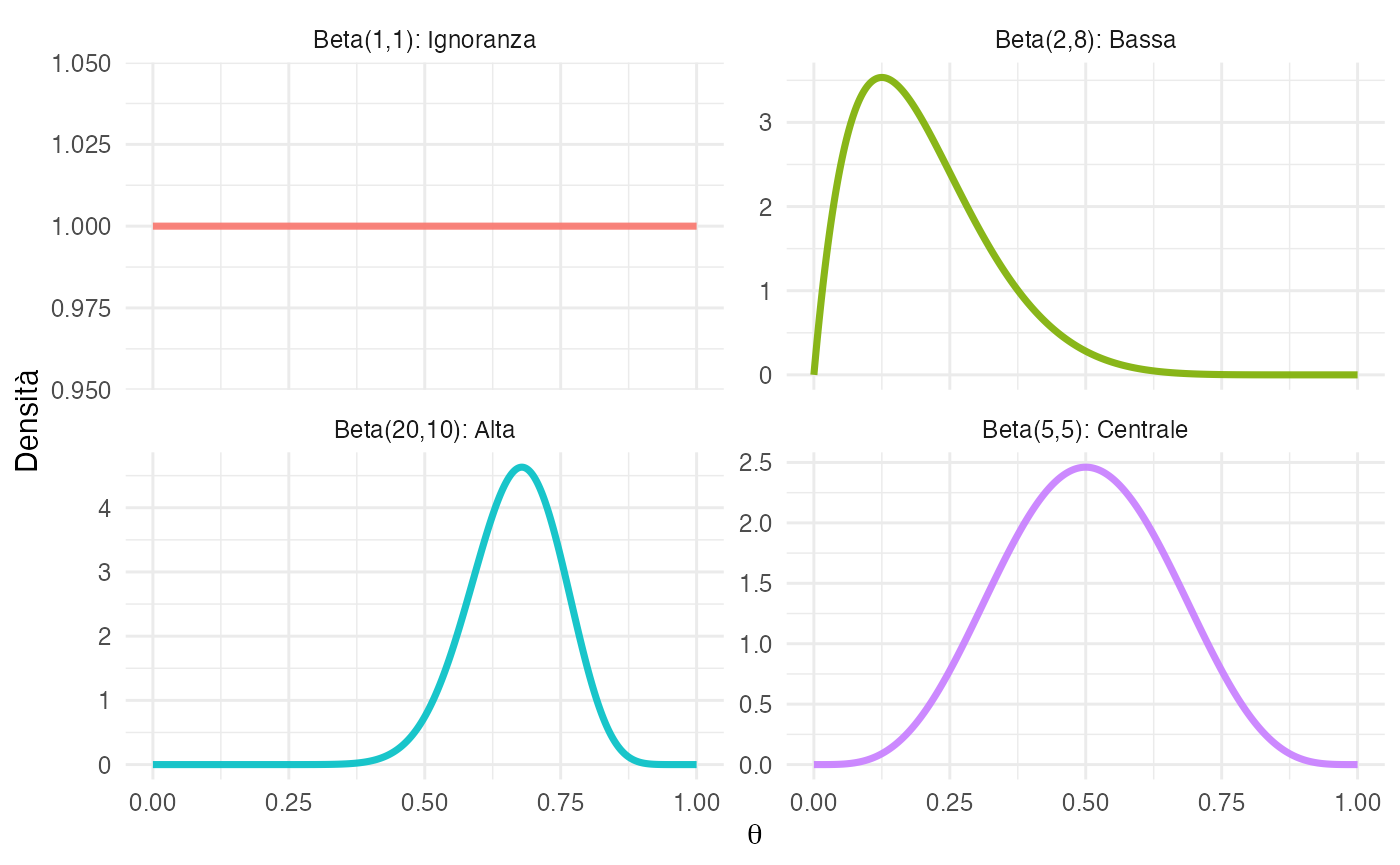
\includegraphics[width=0.85\linewidth,height=\textheight,keepaspectratio]{chapters/probability/03_equiprobability_combinatorics_bayesian_files/figure-pdf/unnamed-chunk-5-1.png}
\end{center}

\subsection{Proprietà fondamentali}\label{proprietuxe0-fondamentali}

\begin{tcolorbox}[enhanced jigsaw, arc=.35mm, breakable, colbacktitle=quarto-callout-tip-color!10!white, opacityback=0, toprule=.15mm, rightrule=.15mm, colback=white, opacitybacktitle=0.6, leftrule=.75mm, coltitle=black, bottomtitle=1mm, left=2mm, toptitle=1mm, title=\textcolor{quarto-callout-tip-color}{\faLightbulb}\hspace{0.5em}{Interpretazione dei parametri}, titlerule=0mm, bottomrule=.15mm, colframe=quarto-callout-tip-color-frame]

\begin{itemize}
\item
  \textbf{Forza delle credenze}: \(\alpha + \beta\). Valori elevati →
  distribuzione concentrata (credenze forti); valori bassi →
  distribuzione diffusa (incertezza elevata).
\item
  \textbf{Posizione (media)}:
  \(\mathbb{E}[\theta] = \frac{\alpha}{\alpha + \beta}\). Indica dove si
  concentra la credenza.
\item
  \textbf{Simmetria}: se \(\alpha = \beta\), la distribuzione è
  simmetrica attorno a 0.5.
\end{itemize}

\end{tcolorbox}

\begin{center}
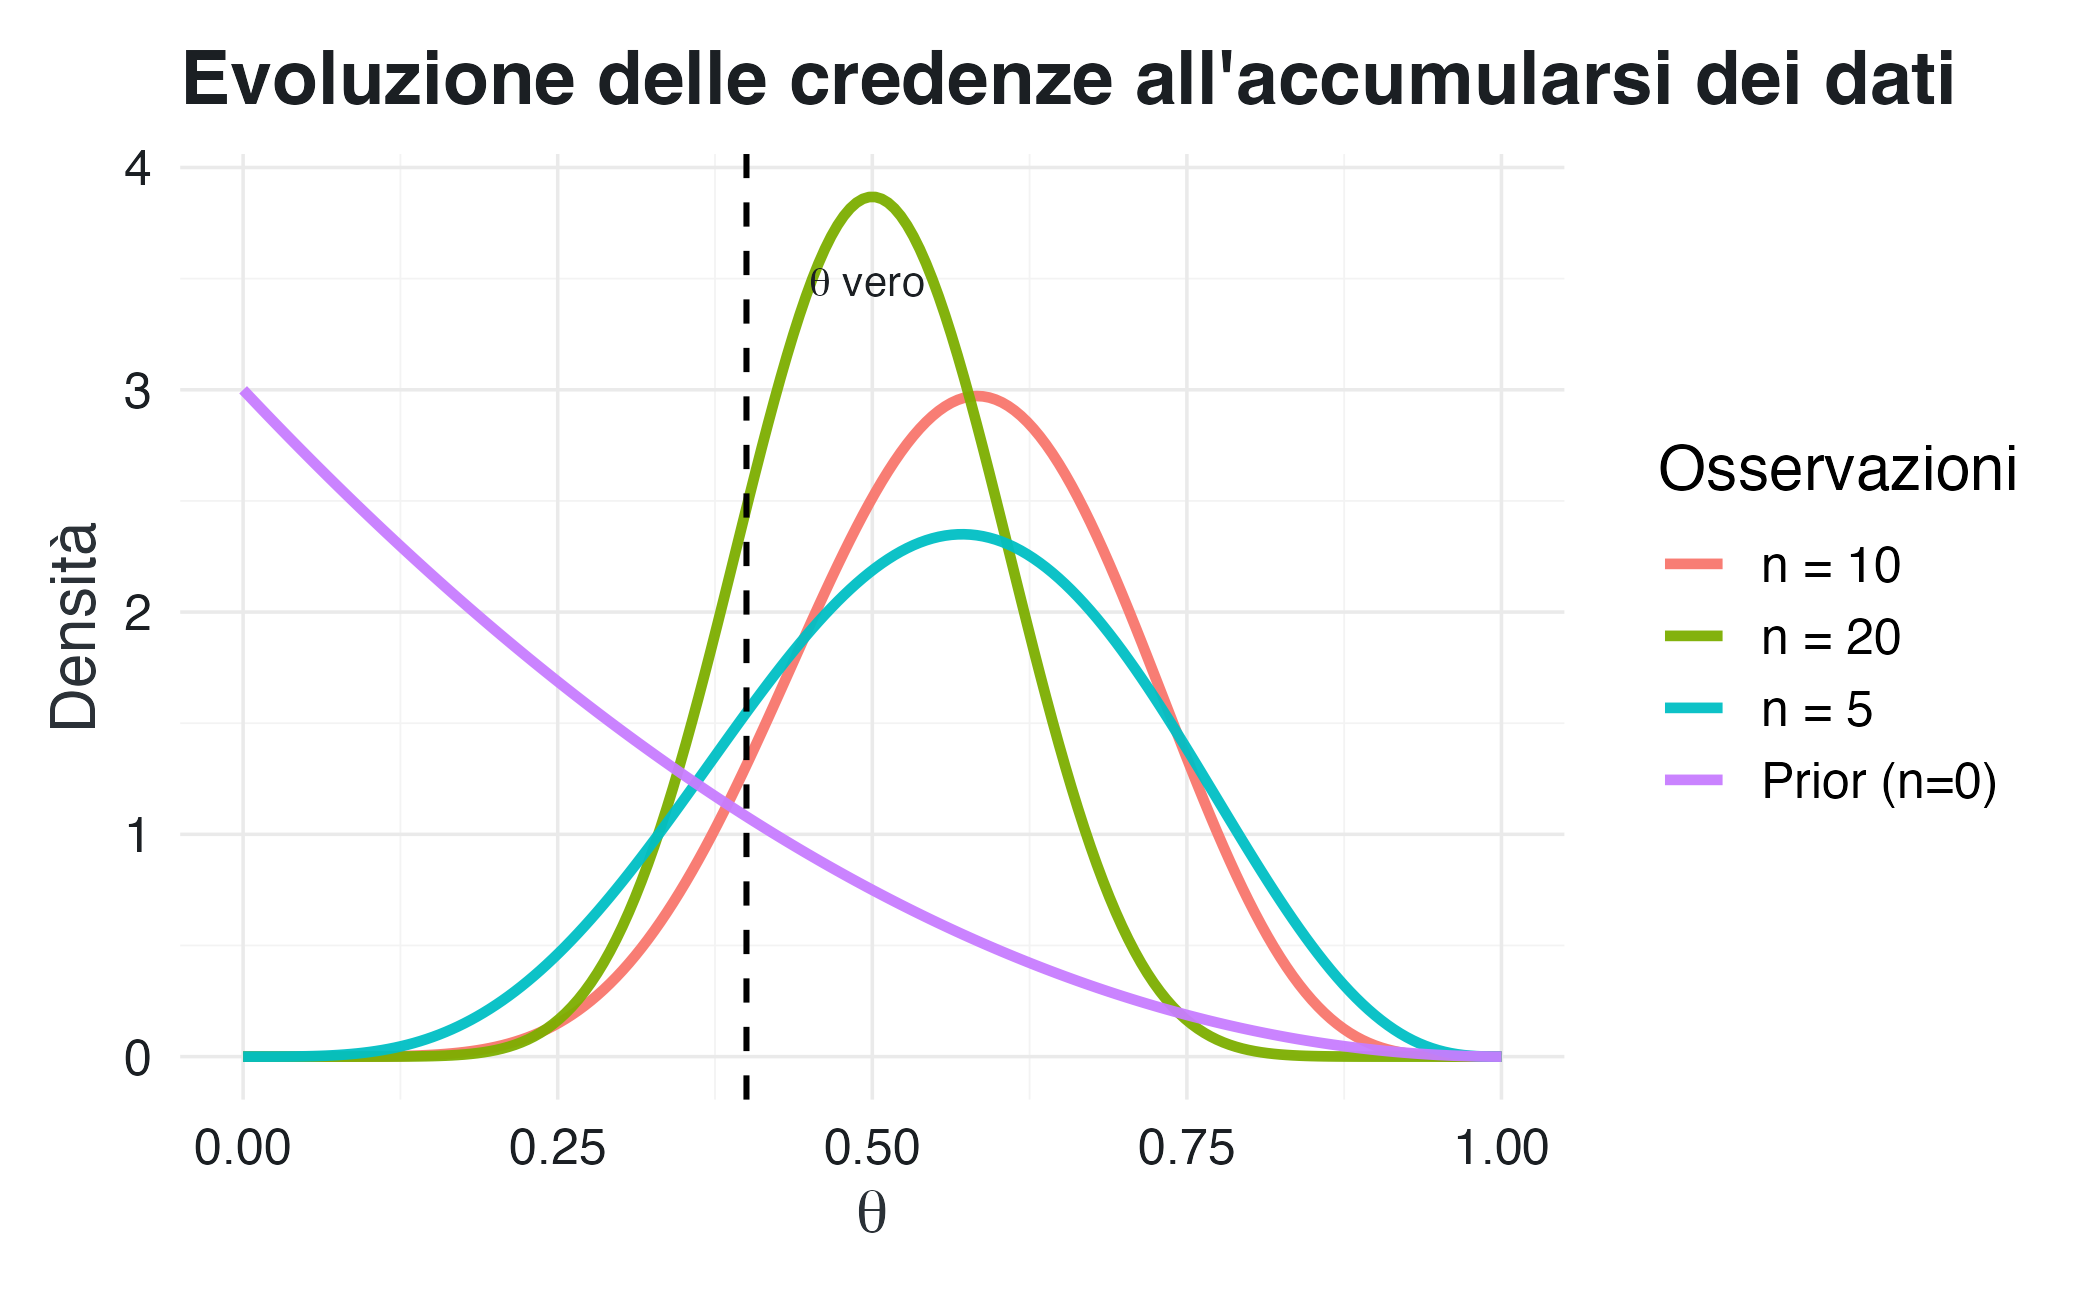
\includegraphics[width=0.85\linewidth,height=\textheight,keepaspectratio]{chapters/probability/03_equiprobability_combinatorics_bayesian_files/figure-pdf/unnamed-chunk-6-1.png}
\end{center}

\subsection{Definizione formale}\label{definizione-formale}

\begin{definition}[]\protect\hypertarget{def-beta-distribution}{}\label{def-beta-distribution}

Una variabile \(\theta \sim \text{Beta}(\alpha, \beta)\) ha densità:

\[
f(\theta; \alpha, \beta) = \frac{\Gamma(\alpha + \beta)}{\Gamma(\alpha)\Gamma(\beta)} \theta^{\alpha-1} (1-\theta)^{\beta-1}, \quad \theta \in [0,1]
\]

\textbf{Proprietà principali}:

\begin{itemize}
\tightlist
\item
  Media: \(\mathbb{E}[\theta] = \frac{\alpha}{\alpha+\beta}\).
\item
  Varianza:
  \(\text{Var}(\theta) = \frac{\alpha\beta}{(\alpha+\beta)^2(\alpha+\beta+1)}\).
\item
  Moda: \(\frac{\alpha-1}{\alpha+\beta-2}\) per \(\alpha, \beta > 1)\).
\end{itemize}

\textbf{Casi notevoli}:

\begin{itemize}
\tightlist
\item
  Beta(1,1) = uniforme su {[}0,1{]} (ignoranza totale)
\item
  Beta(0.5,0.5) = prior di Jeffreys
\end{itemize}

\end{definition}

\subsection{Beta(1,1): la generalizzazione continua
dell'equiprobabilità}\label{beta11-la-generalizzazione-continua-dellequiprobabilituxe0}

La distribuzione Beta(1,1) coincide con la distribuzione uniforme su
{[}0,1{]}: ogni valore di \(\theta\) è ugualmente plausibile. È
l'analogo \textbf{continuo} del principio di indifferenza, estendendo
l'idea di equiprobabilità dal discreto al continuo.

\section{Aggiornamento bayesiano: il modello
Beta-Binomiale}\label{aggiornamento-bayesiano-il-modello-beta-binomiale}

Quando osserviamo \(k\) successi su \(n\) prove binarie, la
distribuzione Beta agisce come \textbf{prior} e viene aggiornata
naturalmente a posteriori secondo la regola di Bayes:

\[
\text{Prior: } \theta \sim \text{Beta}(\alpha, \beta) \quad \Rightarrow \quad \text{Posterior: } \theta \mid k \sim \text{Beta}(\alpha + k, \beta + n - k).
\]

Questa proprietà, nota come \textbf{coniugazione Beta-Binomiale},
permette di aggiornare le credenze in modo semplice e interpretabile.

\subsection{Esempio: test a scelta
multipla}\label{esempio-test-a-scelta-multipla}

Uno studente risponde a 20 domande con 4 opzioni ciascuna. Supponiamo di
avere un prior Beta(1,3), riflettendo l'ipotesi iniziale che le risposte
siano casuali (media 0.25). Se osserviamo 7 risposte corrette, la
posterior diventa:

\[
\text{Posterior: } \theta \sim \text{Beta}(1 + 7, 3 + 13) = \text{Beta}(8, 16).
\]

\begin{itemize}
\tightlist
\item
  \textbf{Media a posteriori}: \(8/24 \approx 0.33\).
\item
  \textbf{Intervallo di credibilità al 95\%}: {[}0.18, 0.52{]}.
\end{itemize}

\begin{Shaded}
\begin{Highlighting}[]
\NormalTok{theta }\OtherTok{\textless{}{-}} \FunctionTok{seq}\NormalTok{(}\DecValTok{0}\NormalTok{, }\DecValTok{1}\NormalTok{, }\AttributeTok{length.out =} \DecValTok{500}\NormalTok{)}
\NormalTok{prior }\OtherTok{\textless{}{-}} \FunctionTok{dbeta}\NormalTok{(theta, }\DecValTok{1}\NormalTok{, }\DecValTok{3}\NormalTok{)}
\NormalTok{posterior }\OtherTok{\textless{}{-}} \FunctionTok{dbeta}\NormalTok{(theta, }\DecValTok{8}\NormalTok{, }\DecValTok{16}\NormalTok{)}

\NormalTok{df }\OtherTok{\textless{}{-}} \FunctionTok{data.frame}\NormalTok{(}
  \AttributeTok{theta =} \FunctionTok{rep}\NormalTok{(theta, }\DecValTok{2}\NormalTok{),}
  \AttributeTok{Densita =} \FunctionTok{c}\NormalTok{(prior, posterior),}
  \AttributeTok{Tipo =} \FunctionTok{rep}\NormalTok{(}\FunctionTok{c}\NormalTok{(}\StringTok{"Prior Beta(1,3)"}\NormalTok{, }\StringTok{"Posterior Beta(8,16)"}\NormalTok{), }\AttributeTok{each =} \DecValTok{500}\NormalTok{)}
\NormalTok{)}

\FunctionTok{ggplot}\NormalTok{(df, }\FunctionTok{aes}\NormalTok{(}\AttributeTok{x =}\NormalTok{ theta, }\AttributeTok{y =}\NormalTok{ Densita, }\AttributeTok{color =}\NormalTok{ Tipo)) }\SpecialCharTok{+}
  \FunctionTok{geom\_line}\NormalTok{(}\AttributeTok{linewidth =} \FloatTok{1.3}\NormalTok{) }\SpecialCharTok{+}
  \FunctionTok{geom\_vline}\NormalTok{(}\AttributeTok{xintercept =} \FunctionTok{c}\NormalTok{(}\FloatTok{0.25}\NormalTok{, }\FloatTok{0.33}\NormalTok{), }\AttributeTok{linetype =} \StringTok{"dashed"}\NormalTok{, }\AttributeTok{alpha =} \FloatTok{0.5}\NormalTok{) }\SpecialCharTok{+}
  \FunctionTok{labs}\NormalTok{(}\AttributeTok{x =} \FunctionTok{expression}\NormalTok{(theta }\SpecialCharTok{\textasciitilde{}} \StringTok{"(probabilità di risposta corretta)"}\NormalTok{),}
       \AttributeTok{y =} \StringTok{"Densità"}\NormalTok{) }\SpecialCharTok{+}
  \FunctionTok{theme\_minimal}\NormalTok{() }
\end{Highlighting}
\end{Shaded}

\begin{center}
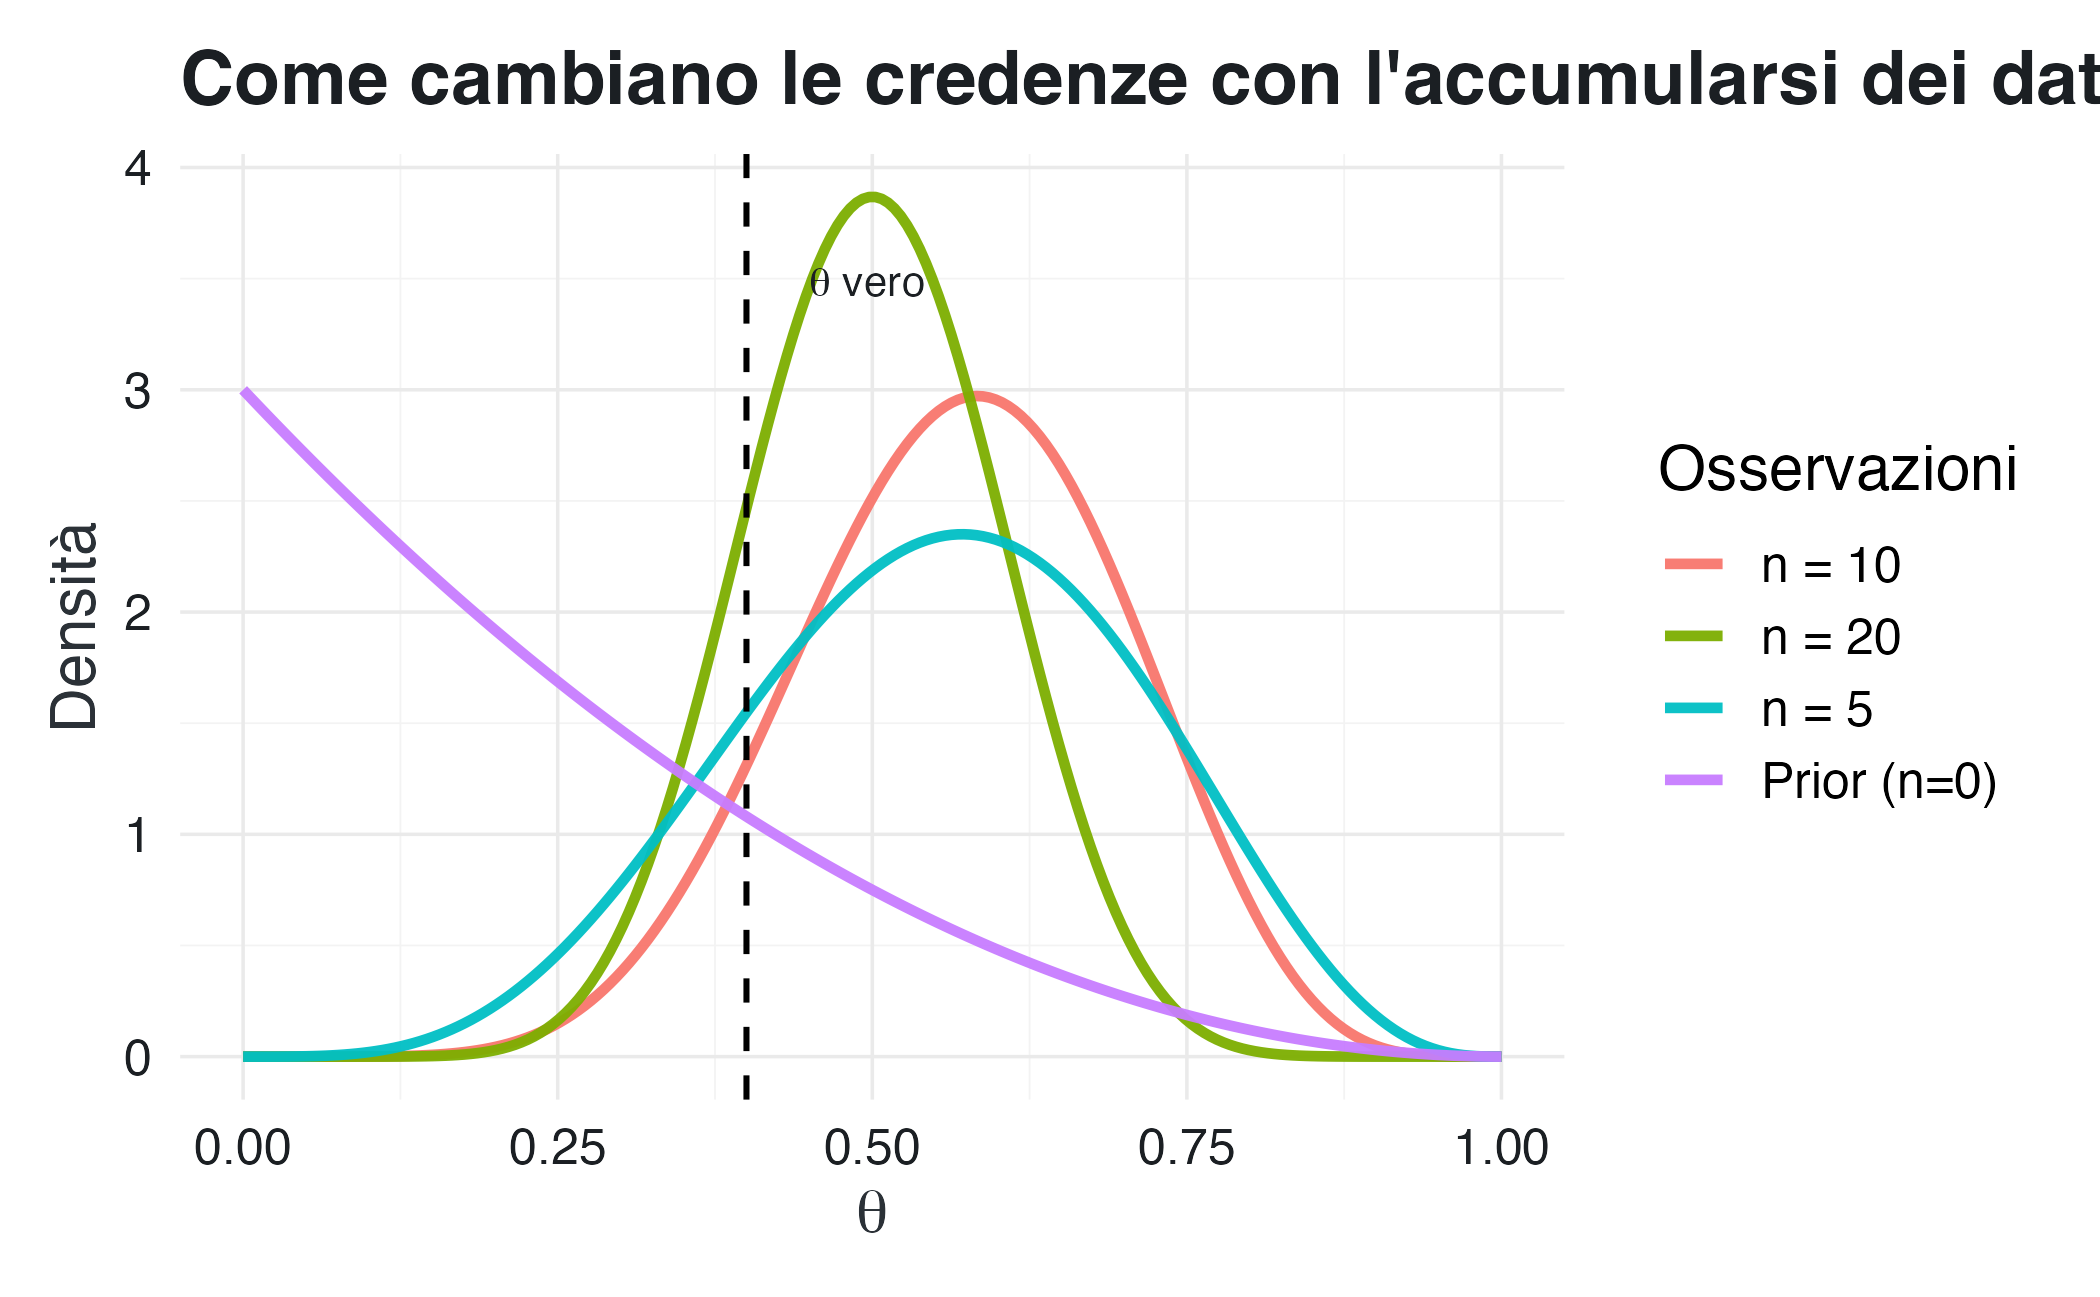
\includegraphics[width=0.85\linewidth,height=\textheight,keepaspectratio]{chapters/probability/03_equiprobability_combinatorics_bayesian_files/figure-pdf/unnamed-chunk-7-1.png}
\end{center}

\subsection{Intervallo di credibilità vs intervallo di
confidenza}\label{intervallo-di-credibilituxe0-vs-intervallo-di-confidenza}

\begin{Shaded}
\begin{Highlighting}[]
\NormalTok{alpha\_post }\OtherTok{\textless{}{-}} \DecValTok{8}
\NormalTok{beta\_post }\OtherTok{\textless{}{-}} \DecValTok{16}
\NormalTok{ci }\OtherTok{\textless{}{-}} \FunctionTok{qbeta}\NormalTok{(}\FunctionTok{c}\NormalTok{(}\FloatTok{0.025}\NormalTok{, }\FloatTok{0.975}\NormalTok{), alpha\_post, beta\_post)}

\FunctionTok{cat}\NormalTok{(}\StringTok{"Media posteriore:"}\NormalTok{, }\FunctionTok{round}\NormalTok{(alpha\_post}\SpecialCharTok{/}\NormalTok{(alpha\_post }\SpecialCharTok{+}\NormalTok{ beta\_post), }\DecValTok{3}\NormalTok{), }\StringTok{"}\SpecialCharTok{\textbackslash{}n}\StringTok{"}\NormalTok{)}
\CommentTok{\#\textgreater{} Media posteriore: 0.333}
\FunctionTok{cat}\NormalTok{(}\StringTok{"IC 95\%: ["}\NormalTok{, }\FunctionTok{round}\NormalTok{(ci[}\DecValTok{1}\NormalTok{], }\DecValTok{2}\NormalTok{), }\StringTok{","}\NormalTok{, }\FunctionTok{round}\NormalTok{(ci[}\DecValTok{2}\NormalTok{], }\DecValTok{2}\NormalTok{), }\StringTok{"]"}\NormalTok{)}
\CommentTok{\#\textgreater{} IC 95\%: [ 0.16 , 0.53 ]}
\end{Highlighting}
\end{Shaded}

\begin{itemize}
\tightlist
\item
  \textbf{Intervallo di credibilità bayesiano (95\%)}: ``C'è il 95\% di
  probabilità che \(\theta\) cada in questo intervallo dato ciò che
  sappiamo.''
\item
  \textbf{Intervallo di confidenza frequentista (95\%)}: ``Se
  ripetessimo l'esperimento infinite volte, il 95\% degli intervalli
  calcolati così conterrebbe il parametro vero.''
\end{itemize}

\subsection{Aggiornamento sequenziale: accumulare
dati}\label{aggiornamento-sequenziale-accumulare-dati}

Il modello Beta-Binomiale permette di aggiornare le credenze \textbf{man
mano che arrivano nuove osservazioni}, senza dover ricalcolare da zero:

\begin{Shaded}
\begin{Highlighting}[]
\FunctionTok{set.seed}\NormalTok{(}\DecValTok{42}\NormalTok{)}
\NormalTok{theta\_vero }\OtherTok{\textless{}{-}} \FloatTok{0.4}
\NormalTok{n\_domande }\OtherTok{\textless{}{-}} \DecValTok{20}
\NormalTok{risposte }\OtherTok{\textless{}{-}} \FunctionTok{rbinom}\NormalTok{(n\_domande, }\DecValTok{1}\NormalTok{, theta\_vero)}

\NormalTok{alpha }\OtherTok{\textless{}{-}} \DecValTok{1}\NormalTok{; beta }\OtherTok{\textless{}{-}} \DecValTok{3}
\NormalTok{theta\_grid }\OtherTok{\textless{}{-}} \FunctionTok{seq}\NormalTok{(}\DecValTok{0}\NormalTok{, }\DecValTok{1}\NormalTok{, }\AttributeTok{length.out =} \DecValTok{200}\NormalTok{)}

\NormalTok{df\_evol }\OtherTok{\textless{}{-}} \FunctionTok{data.frame}\NormalTok{()}
\ControlFlowTok{for}\NormalTok{(i }\ControlFlowTok{in} \FunctionTok{c}\NormalTok{(}\DecValTok{0}\NormalTok{, }\DecValTok{5}\NormalTok{, }\DecValTok{10}\NormalTok{, }\DecValTok{20}\NormalTok{)) \{}
  \ControlFlowTok{if}\NormalTok{(i }\SpecialCharTok{==} \DecValTok{0}\NormalTok{) \{}
\NormalTok{    dens }\OtherTok{\textless{}{-}} \FunctionTok{dbeta}\NormalTok{(theta\_grid, alpha, beta)}
\NormalTok{  \} }\ControlFlowTok{else}\NormalTok{ \{}
\NormalTok{    a }\OtherTok{\textless{}{-}} \DecValTok{1} \SpecialCharTok{+} \FunctionTok{sum}\NormalTok{(risposte[}\DecValTok{1}\SpecialCharTok{:}\NormalTok{i])}
\NormalTok{    b }\OtherTok{\textless{}{-}} \DecValTok{3} \SpecialCharTok{+}\NormalTok{ i }\SpecialCharTok{{-}} \FunctionTok{sum}\NormalTok{(risposte[}\DecValTok{1}\SpecialCharTok{:}\NormalTok{i])}
\NormalTok{    dens }\OtherTok{\textless{}{-}} \FunctionTok{dbeta}\NormalTok{(theta\_grid, a, b)}
\NormalTok{  \}}
\NormalTok{  df\_evol }\OtherTok{\textless{}{-}} \FunctionTok{rbind}\NormalTok{(df\_evol, }\FunctionTok{data.frame}\NormalTok{(}
    \AttributeTok{theta =}\NormalTok{ theta\_grid, }\AttributeTok{Densita =}\NormalTok{ dens, }\AttributeTok{n =} \FunctionTok{paste0}\NormalTok{(}\StringTok{"n = "}\NormalTok{, i)}
\NormalTok{  ))}
\NormalTok{\}}

\FunctionTok{ggplot}\NormalTok{(df\_evol, }\FunctionTok{aes}\NormalTok{(}\AttributeTok{x =}\NormalTok{ theta, }\AttributeTok{y =}\NormalTok{ Densita, }\AttributeTok{color =}\NormalTok{ n)) }\SpecialCharTok{+}
  \FunctionTok{geom\_line}\NormalTok{(}\AttributeTok{linewidth =} \FloatTok{1.2}\NormalTok{) }\SpecialCharTok{+}
  \FunctionTok{geom\_vline}\NormalTok{(}\AttributeTok{xintercept =}\NormalTok{ theta\_vero, }\AttributeTok{linetype =} \StringTok{"dashed"}\NormalTok{) }\SpecialCharTok{+}
  \FunctionTok{annotate}\NormalTok{(}\StringTok{"text"}\NormalTok{, }\AttributeTok{x =}\NormalTok{ theta\_vero }\SpecialCharTok{+} \FloatTok{0.05}\NormalTok{, }\AttributeTok{y =} \FunctionTok{max}\NormalTok{(df\_evol}\SpecialCharTok{$}\NormalTok{Densita) }\SpecialCharTok{*} \FloatTok{0.9}\NormalTok{,}
           \AttributeTok{label =} \FunctionTok{expression}\NormalTok{(theta}\SpecialCharTok{\textasciitilde{}}\NormalTok{vero), }\AttributeTok{hjust =} \DecValTok{0}\NormalTok{) }\SpecialCharTok{+}
  \FunctionTok{labs}\NormalTok{(}\AttributeTok{x =} \FunctionTok{expression}\NormalTok{(theta), }\AttributeTok{y =} \StringTok{"Densità"}\NormalTok{, }\AttributeTok{color =} \StringTok{"Numero di osservazioni"}\NormalTok{) }\SpecialCharTok{+}
  \FunctionTok{theme\_minimal}\NormalTok{()}
\end{Highlighting}
\end{Shaded}

\begin{center}
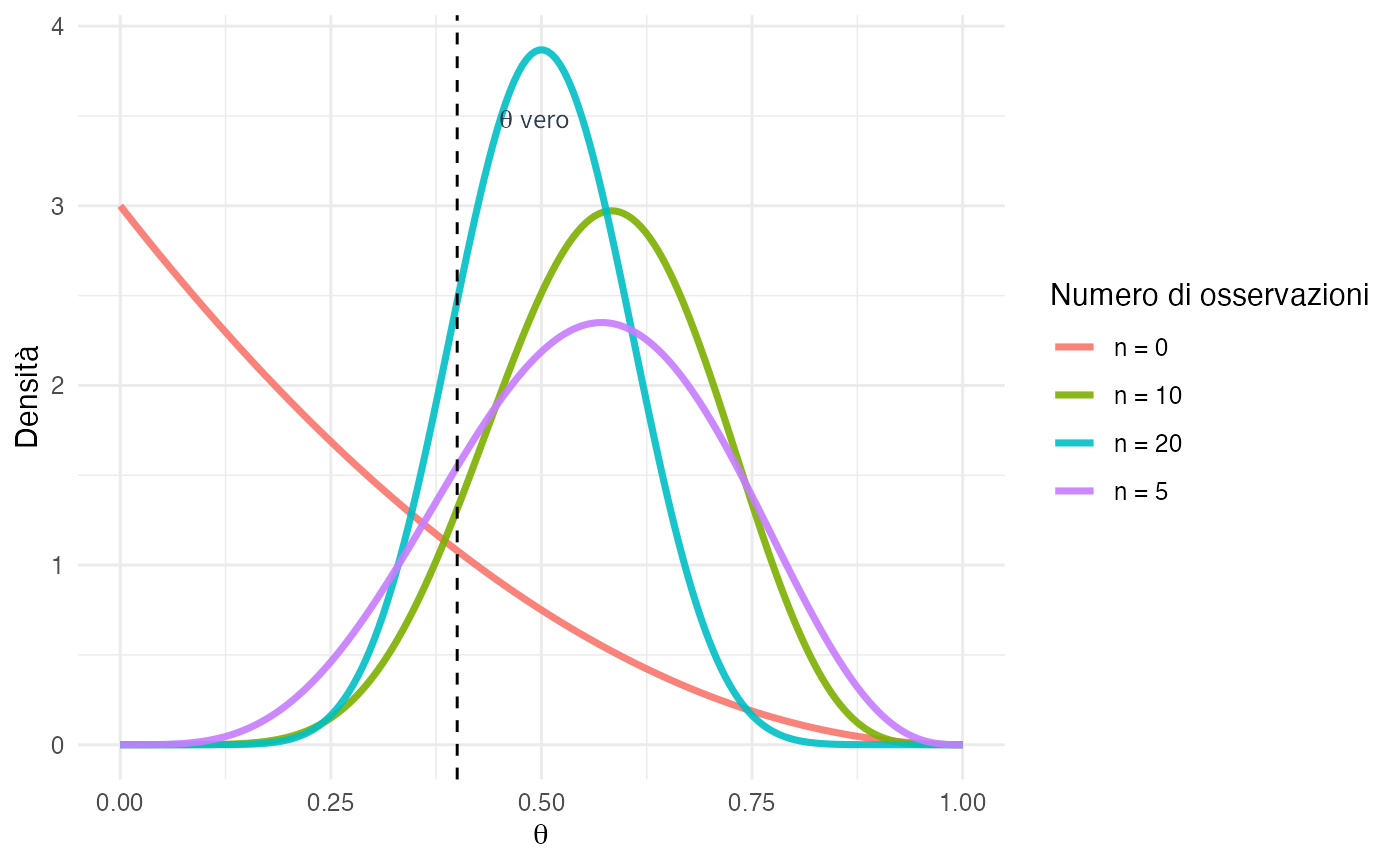
\includegraphics[width=0.85\linewidth,height=\textheight,keepaspectratio]{chapters/probability/03_equiprobability_combinatorics_bayesian_files/figure-pdf/unnamed-chunk-9-1.png}
\end{center}

\textbf{Interpretazione}: con l'accumularsi delle prove, la
distribuzione posterior si concentra attorno al valore reale
\(\theta_\text{vero}\), riflettendo una crescente certezza nelle stime.
Questo esempio mostra in modo chiaro come l'inferenza bayesiana integri
informazioni pregresse (\emph{prior}) con dati osservati, fornendo stime
aggiornate e interpretabili in termini probabilistici.

\section{Applicazioni psicologiche}\label{applicazioni-psicologiche}

\subsection{Item Response Theory (IRT)}\label{item-response-theory-irt}

Nella psicologia dell'apprendimento, la probabilità di rispondere
correttamente a un item non è uniforme, ma dipende dall'abilità dello
studente (\(\theta\)) e dalla difficoltà dell'item (\(b\)). La
\textbf{Item Response Theory (IRT)} descrive questa relazione tramite un
modello logit:

\[
P(\text{corretto} \mid \theta, b) = \frac{1}{1 + e^{-(\theta - b)}}
\]

In questo modo, gli item più facili hanno alte probabilità di risposta
corretta anche per gli studenti con abilità basse, mentre gli item più
difficili permettono di distinguere meglio gli studenti più preparati.
Questo approccio riflette la variabilità sistematica presente nei dati
psicometrici e mostra quanto sia artificiale assumere l'equiprobabilità.

\subsection{Bias di risposta nei
questionari}\label{bias-di-risposta-nei-questionari}

Nei questionari, le risposte non seguono un modello equiprobabile.
Fenomeni come l'acquiescenza, la desiderabilità sociale o gli stili
individuali influenzano la probabilità di selezionare determinate
opzioni. Anche in questo caso, la probabilità di risposta varia in modo
sistematico e può essere stimata formalmente utilizzando metodi
bayesiani che integrano conoscenze pregresse e dati osservati.

\subsection{Efficacia di interventi}\label{efficacia-di-interventi}

Quando si valutano gli interventi psicologici, come la terapia
cognitivo-comportamentale, la probabilità di successo non è uguale per
tutti i partecipanti. L'approccio bayesiano consente di combinare le
informazioni preesistenti (ad esempio, i risultati di studi precedenti)
con i dati raccolti nello studio corrente, aggiornando le credenze sulla
reale efficacia del trattamento. Ciò fornisce stime più precise e
interpretabili in termini probabilistici, mettendo in luce la naturale
variabilità tra individui e contesti.

\section*{Riflessioni conclusive}\label{riflessioni-conclusive-2}

\markright{Riflessioni conclusive}

L'equiprobabilità non è una proprietà intrinseca del mondo, ma riflette
uno stato di \textbf{ignoranza simmetrica}: consideriamo tutti i casi
elementari come ugualmente plausibili solo quando non abbiamo alcuna
ragione per privilegiare uno rispetto a un altro. La famosa formula
``casi favorevoli su casi possibili'' non è quindi una legge universale
della probabilità, ma un caso particolare che si applica solo in
presenza di questa condizione di simmetria.

Il calcolo combinatorio può essere reso coerente con il framework
bayesiano ipotizzando l'equiprobabilità solo in questi contesti. Le
combinazioni, le disposizioni e le altre formule di conteggio non
costituiscono teorie indipendenti della probabilità, ma sono strumenti
di modellazione che implicano l'equiprobabilità di ogni evento
elementare. Quando questa ipotesi non è giustificata, come spesso accade
nelle scienze psicologiche e sociali, è necessario ricorrere a modelli
più flessibili che siano in grado di rappresentare differenze
sistematiche tra eventi o informazioni pregresse.

La distribuzione Beta fornisce una generalizzazione continua di questo
concetto. La distribuzione Beta(1,1) rappresenta lo stato di massima
ignoranza, ovvero l'equiprobabilità generalizzata, mentre altri valori
dei parametri permettono di codificare credenze a priori con forme e
intensità diverse. L'aggiornamento bayesiano offre infine un meccanismo
coerente per spiegare come queste credenze possono evolvere nel tempo:
combinando conoscenze pregresse ed evidenza empirica, consente di
modulare le probabilità man mano che i dati si accumulano, integrando in
un unico processo logico l'esperienza e l'incertezza.

\chapter{Probabilità condizionata come
aggiornamento}\label{sec-prob-conditional-prob}

\section*{Introduzione}\label{introduzione-4}

\markright{Introduzione}

La probabilità condizionata rappresenta il meccanismo fondamentale
attraverso il quale le credenze si aggiornano in modo coerente alla luce
di nuove informazioni. Quando apprendiamo che si è verificato un evento
\(B\), la nostra valutazione della plausibilità di un evento \(A\)
subisce una trasformazione sistematica quantificata dalla probabilità
condizionata \(P(A|B)\).

Dal punto di vista bayesiano, ogni assegnazione probabilistica è
implicitamente condizionata dallo stato informativo disponibile.
L'espressione \(P(A)\) è in realtà una forma abbreviata di
\(P(A \mid \mathcal{I})\), dove \(\mathcal{I}\) rappresenta l'insieme
delle conoscenze attualmente possedute. La probabilità condizionata
formalizza matematicamente il processo di riduzione dello spazio
epistemico: l'acquisizione dell'informazione B restringe l'insieme delle
possibilità a quelle compatibili con tale evidenza, richiedendo una
ricalibrazione coerente delle credenze.

In questo capitolo esploreremo la probabilità condizionata non come una
semplice operazione insiemistica, ma come un principio di coerenza per
l'aggiornamento razionale delle credenze. Esamineremo come questo
concetto fondamentale sia essenziale per comprendere nozioni quali
l'indipendenza probabilistica, il teorema del prodotto, la legge della
probabilità totale e, nel capitolo successivo, il teorema di Bayes.

\subsection*{Panoramica del capitolo}\label{panoramica-del-capitolo-3}

\begin{itemize}
\tightlist
\item
  Probabilità condizionata come riduzione dello spazio epistemico.
\item
  Interpretazione epistemica dell'aggiornamento.
\item
  Indipendenza come assenza di informazione reciproca.
\item
  Teorema del prodotto e probabilità congiunta.
\item
  Legge della probabilità totale.
\item
  Paradosso di Simpson.
\item
  Applicazioni a diagnostica clinica e test psicologici.
\end{itemize}

\begin{tcolorbox}[enhanced jigsaw, arc=.35mm, breakable, colbacktitle=quarto-callout-tip-color!10!white, opacityback=0, toprule=.15mm, rightrule=.15mm, colback=white, opacitybacktitle=0.6, leftrule=.75mm, coltitle=black, bottomtitle=1mm, left=2mm, toptitle=1mm, title=\textcolor{quarto-callout-tip-color}{\faLightbulb}\hspace{0.5em}{Prerequisiti}, titlerule=0mm, bottomrule=.15mm, colframe=quarto-callout-tip-color-frame]

\begin{itemize}
\tightlist
\item
  Aver letto i capitoli precedenti
  (Chapter~\ref{sec-prob-interpretation}, \textbf{?@sec-prob-models},
  Chapter~\ref{sec-equiprobability-combinatorics}).
\item
  Familiarità con tabelle congiunte.
\item
  Nozioni base di R per simulazioni.
\end{itemize}

\end{tcolorbox}

\begin{tcolorbox}[enhanced jigsaw, arc=.35mm, breakable, colbacktitle=quarto-callout-caution-color!10!white, opacityback=0, toprule=.15mm, rightrule=.15mm, colback=white, opacitybacktitle=0.6, leftrule=.75mm, coltitle=black, bottomtitle=1mm, left=2mm, toptitle=1mm, title=\textcolor{quarto-callout-caution-color}{\faFire}\hspace{0.5em}{Preparazione del Notebook}, titlerule=0mm, bottomrule=.15mm, colframe=quarto-callout-caution-color-frame]

\begin{Shaded}
\begin{Highlighting}[]
\NormalTok{here}\SpecialCharTok{::}\FunctionTok{here}\NormalTok{(}\StringTok{"code"}\NormalTok{, }\StringTok{"\_common.R"}\NormalTok{) }\SpecialCharTok{|\textgreater{}} 
  \FunctionTok{source}\NormalTok{()}

\CommentTok{\# Load packages}
\ControlFlowTok{if}\NormalTok{ (}\SpecialCharTok{!}\FunctionTok{requireNamespace}\NormalTok{(}\StringTok{"pacman"}\NormalTok{)) }\FunctionTok{install.packages}\NormalTok{(}\StringTok{"pacman"}\NormalTok{)}
\NormalTok{pacman}\SpecialCharTok{::}\FunctionTok{p\_load}\NormalTok{(ggplot2, dplyr, tidyr, patchwork, ggforce, DiagrammeR)}
\end{Highlighting}
\end{Shaded}

\end{tcolorbox}

\section{Definizione e interpretazione
epistemica}\label{definizione-e-interpretazione-epistemica}

\begin{definition}[Probabilità
condizionata]\protect\hypertarget{def-conditional-probability}{}\label{def-conditional-probability}

Se \(P(B) > 0\), la \emph{probabilità condizionata} di \(A\) dato \(B\)
è definita come:

\begin{equation}\phantomsection\label{eq-prob-cond-def}{
P(A \mid B) = \frac{P(A \cap B)}{P(B)}
}\end{equation}

\textbf{Interpretazione epistemica}: \(P(A \mid B)\) quantifica il
nostro grado di credenza in \(A\) dopo aver appreso che \(B\) è vero,
tenendo conto del fatto che ora lo spazio delle possibilità si è
ristretto a quelle compatibili con \(B\).

\end{definition}

\subsection{Fondamento logico della
formula}\label{fondamento-logico-della-formula}

La definizione di probabilità condizionata non costituisce una
convenzione arbitraria, ma emerge come necessaria conseguenza del
principio di coerenza probabilistica. Consideriamo una distribuzione di
probabilità congiunta rappresentata da una tabella 2×2. Quando
apprendiamo che l'evento \(B\) si è verificato, lo spazio probabilistico
si riduce alla sola colonna corrispondente a \(B\). Per preservare la
coerenza interna del nostro sistema di credenze, dobbiamo eliminare
tutti gli esiti incompatibili con \(B\) e rinormalizzare le credenze
residue assicurando che la probabilità totale dello spazio ridotto sia
pari a 1. Questa rinormalizzazione si ottiene dividendo ciascuna
probabilità residua per \(P(B)\).

Il risultato di questo processo è la formula della probabilità
condizionata: \[
P(A \mid B) = \frac{P(A \cap B)}{P(B)}.
\]

\begin{tcolorbox}[enhanced jigsaw, arc=.35mm, breakable, colbacktitle=quarto-callout-important-color!10!white, opacityback=0, toprule=.15mm, rightrule=.15mm, colback=white, opacitybacktitle=0.6, leftrule=.75mm, coltitle=black, bottomtitle=1mm, left=2mm, toptitle=1mm, title=\textcolor{quarto-callout-important-color}{\faExclamation}\hspace{0.5em}{Principio epistemico fondamentale}, titlerule=0mm, bottomrule=.15mm, colframe=quarto-callout-important-color-frame]

\subsubsection*{Aggiornamento come riduzione e
rinormalizzazione}\label{aggiornamento-come-riduzione-e-rinormalizzazione}

L'acquisizione dell'informazione che l'evento \(B\) si è verificato
innesca un processo di aggiornamento epistemico strutturato in tre fasi
fondamentali. In primo luogo, si verifica una riduzione dello spazio
epistemico dall'intero universo \(\Omega\) al sottoinsieme \(B\),
eliminando tutte le possibilità incompatibili con l'evidenza osservata.
In secondo luogo, si procede a una rinominalizzazione delle credenze su
questo sottospazio ridotto, garantendo che le probabilità assegnate agli
eventi rimanenti sommino nuovamente a 1. In terzo luogo, le proporzioni
relative tra tutti gli eventi compatibili con \(B\) rimangono
inalterate, preservando la struttura delle relazioni probabilistiche
originarie.

Questo meccanismo garantisce la coerenza epistemica: se avessimo
inizialmente considerato esclusivamente \(B\) come nostro spazio di
possibilità, avremmo ottenuto le stesse credenze relative agli eventi
risultanti dal processo di aggiornamento condizionale.

\end{tcolorbox}

\subsection{Visualizzazione
geometrica}\label{visualizzazione-geometrica}

\begin{Shaded}
\begin{Highlighting}[]
\CommentTok{\# Esempio con diagramma di Venn simulato}
\CommentTok{\# Parametri}
\NormalTok{P\_A }\OtherTok{\textless{}{-}} \FloatTok{0.6}
\NormalTok{P\_B }\OtherTok{\textless{}{-}} \FloatTok{0.5}
\NormalTok{P\_AB }\OtherTok{\textless{}{-}} \FloatTok{0.35}

\CommentTok{\# Creare dataframe per visualizzazione}
\NormalTok{df\_venn }\OtherTok{\textless{}{-}} \FunctionTok{data.frame}\NormalTok{(}
  \AttributeTok{x =} \FunctionTok{c}\NormalTok{(}\FloatTok{0.3}\NormalTok{, }\FloatTok{0.7}\NormalTok{),}
  \AttributeTok{y =} \FunctionTok{c}\NormalTok{(}\FloatTok{0.5}\NormalTok{, }\FloatTok{0.5}\NormalTok{),}
  \AttributeTok{r =} \FunctionTok{c}\NormalTok{(}\FunctionTok{sqrt}\NormalTok{(P\_A }\SpecialCharTok{/}\NormalTok{ pi), }\FunctionTok{sqrt}\NormalTok{(P\_B }\SpecialCharTok{/}\NormalTok{ pi)),}
  \AttributeTok{label =} \FunctionTok{c}\NormalTok{(}\StringTok{"A"}\NormalTok{, }\StringTok{"B"}\NormalTok{)}
\NormalTok{)}

\CommentTok{\# Calcolare condizionata}
\NormalTok{P\_A\_given\_B }\OtherTok{\textless{}{-}}\NormalTok{ P\_AB }\SpecialCharTok{/}\NormalTok{ P\_B}

\FunctionTok{ggplot}\NormalTok{() }\SpecialCharTok{+}
  \FunctionTok{geom\_circle}\NormalTok{(}\AttributeTok{data =}\NormalTok{ df\_venn, }\FunctionTok{aes}\NormalTok{(}\AttributeTok{x0 =}\NormalTok{ x, }\AttributeTok{y0 =}\NormalTok{ y, }\AttributeTok{r =}\NormalTok{ r, }\AttributeTok{fill =}\NormalTok{ label), }
              \AttributeTok{alpha =} \FloatTok{0.3}\NormalTok{, }\AttributeTok{size =} \DecValTok{1}\NormalTok{, }\AttributeTok{show.legend =} \ConstantTok{FALSE}\NormalTok{) }\SpecialCharTok{+}
  \FunctionTok{annotate}\NormalTok{(}\StringTok{"text"}\NormalTok{, }\AttributeTok{x =} \FloatTok{0.3}\NormalTok{, }\AttributeTok{y =} \FloatTok{0.85}\NormalTok{, }\AttributeTok{label =} \StringTok{"A"}\NormalTok{, }\AttributeTok{size =} \DecValTok{8}\NormalTok{) }\SpecialCharTok{+}
  \FunctionTok{annotate}\NormalTok{(}\StringTok{"text"}\NormalTok{, }\AttributeTok{x =} \FloatTok{0.7}\NormalTok{, }\AttributeTok{y =} \FloatTok{0.85}\NormalTok{, }\AttributeTok{label =} \StringTok{"B"}\NormalTok{, }\AttributeTok{size =} \DecValTok{8}\NormalTok{) }\SpecialCharTok{+}
  \FunctionTok{annotate}\NormalTok{(}\StringTok{"text"}\NormalTok{, }\AttributeTok{x =} \FloatTok{0.5}\NormalTok{, }\AttributeTok{y =} \FloatTok{0.5}\NormalTok{, }\AttributeTok{label =} \StringTok{"A ∩ B"}\NormalTok{, }\AttributeTok{size =} \DecValTok{6}\NormalTok{) }\SpecialCharTok{+}
  \FunctionTok{annotate}\NormalTok{(}\StringTok{"text"}\NormalTok{, }\AttributeTok{x =} \FloatTok{0.5}\NormalTok{, }\AttributeTok{y =} \SpecialCharTok{{-}}\FloatTok{0.1}\NormalTok{, }
           \AttributeTok{label =} \FunctionTok{sprintf}\NormalTok{(}\StringTok{"P(A|B) = P(A∩B)/P(B) = \%.2f/\%.2f = \%.2f"}\NormalTok{, }
\NormalTok{                          P\_AB, P\_B, P\_A\_given\_B),}
           \AttributeTok{size =} \DecValTok{5}\NormalTok{) }\SpecialCharTok{+}
  \FunctionTok{coord\_fixed}\NormalTok{() }\SpecialCharTok{+}
  \FunctionTok{theme\_void}\NormalTok{() }\SpecialCharTok{+}
  \FunctionTok{labs}\NormalTok{(}\AttributeTok{title =} \StringTok{"Probabilità condizionata come riduzione dello spazio"}\NormalTok{,}
       \AttributeTok{subtitle =} \StringTok{"Apprendere B significa focalizzarsi sulla regione B e rinormalizzare"}\NormalTok{)}
\end{Highlighting}
\end{Shaded}

\begin{center}
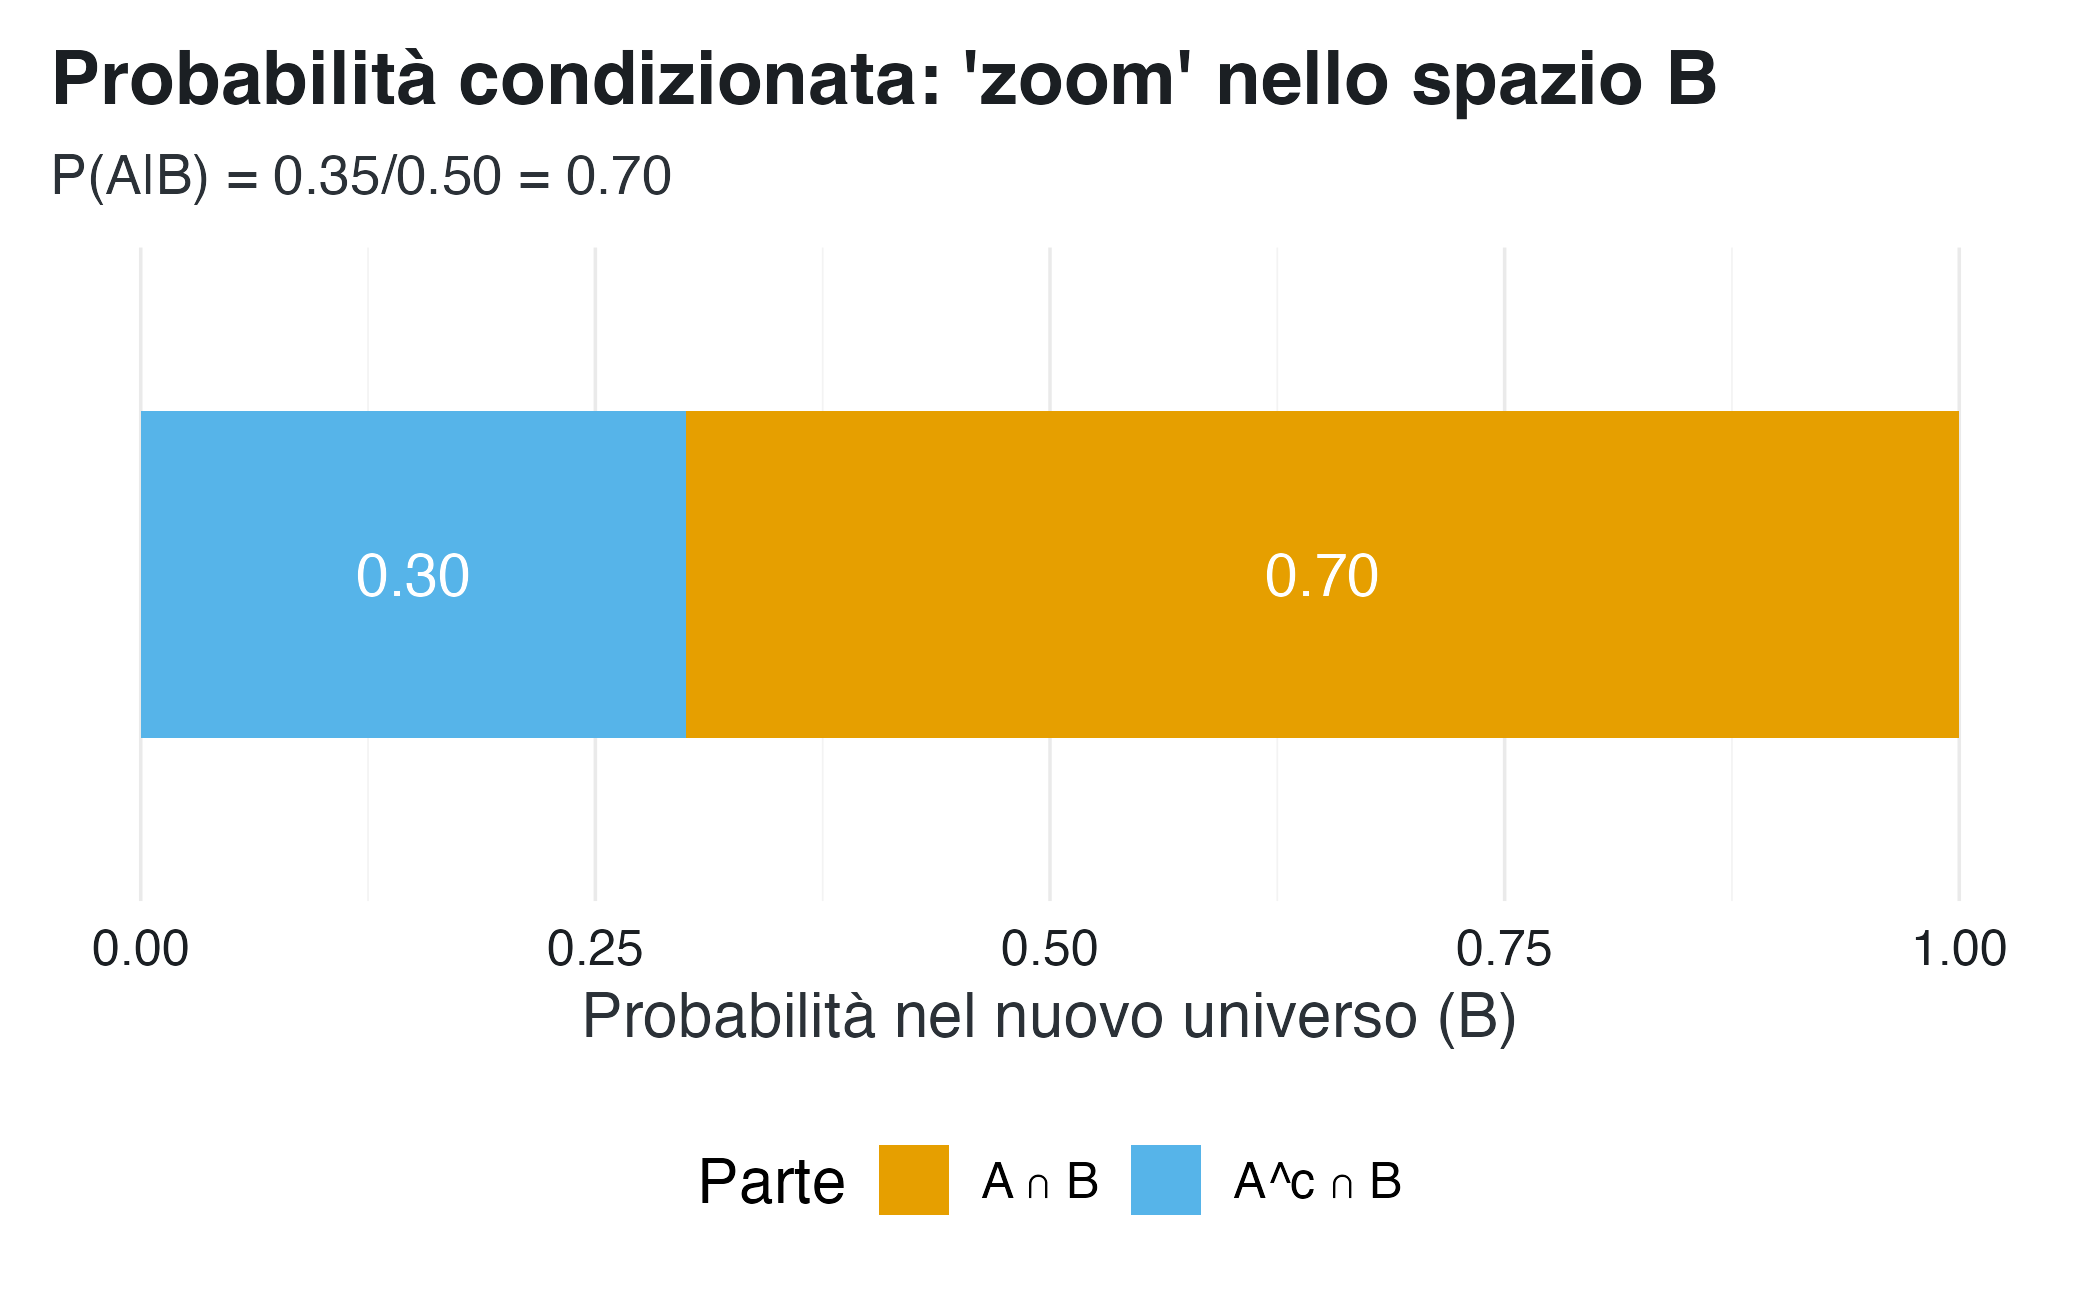
\includegraphics[width=0.85\linewidth,height=\textheight,keepaspectratio]{chapters/probability/04_conditional_prob_bayesian_files/figure-pdf/unnamed-chunk-2-1.png}
\end{center}

\section{Proprietà della probabilità
condizionata}\label{proprietuxe0-della-probabilituxe0-condizionata}

Le probabilità condizionate mantengono le proprietà degli assiomi,
trattando \(B\) come nuovo ``universo''.

\begin{theorem}[Proprietà della
condizionata]\protect\hypertarget{thm-conditional-properties}{}\label{thm-conditional-properties}

Fissato un evento \(B\) con \(P(B) > 0\), la funzione
\(P(\cdot \mid B)\) soddisfa tutti gli assiomi della probabilità.

\begin{enumerate}
\def\labelenumi{\arabic{enumi}.}
\item
  \textbf{Non-negatività}: \(P(A \mid B) \geq 0\) per ogni evento \(A\).
\item
  \textbf{Normalizzazione}: \(P(B \mid B) = 1\) (certezza di \(B\) dato
  \(B\)).
\item
  \textbf{Additività}: se \(A_1, A_2\) sono eventi disgiunti, allora
  \[P(A_1 \cup A_2 \mid B) = P(A_1 \mid B) + P(A_2 \mid B).\]
\item
  \textbf{Complemento}: \(P(A^c \mid B) = 1 - P(A \mid B).\)
\item
  \textbf{Regola della catena (o del prodotto)}:
  \[P(A \cap B \mid C) = P(A \mid B \cap C) \cdot P(B \mid C).\]
\end{enumerate}

\end{theorem}

La dimostrazione della proprietà di additività si fonda sulla
disgiunzione degli eventi: poiché \(A_1\) e \(A_2\) sono disgiunti,
anche le loro intersezioni con \(B\) risultano disgiunte, permettendo di
applicare l'assioma di additività al numeratore.

\begin{tcolorbox}[enhanced jigsaw, arc=.35mm, breakable, colbacktitle=quarto-callout-note-color!10!white, opacityback=0, toprule=.15mm, rightrule=.15mm, colback=white, opacitybacktitle=0.6, leftrule=.75mm, coltitle=black, bottomtitle=1mm, left=2mm, toptitle=1mm, title=\textcolor{quarto-callout-note-color}{\faInfo}\hspace{0.5em}{Esempio clinico completo}, titlerule=0mm, bottomrule=.15mm, colframe=quarto-callout-note-color-frame]

\subsubsection*{Test di screening per il disturbo depressivo
maggiore}\label{test-di-screening-per-il-disturbo-depressivo-maggiore}

\textbf{Contesto clinico}: uno psicologo utilizza un test di screening
per il disturbo depressivo maggiore in un contesto di comunità,
caratterizzato da una popolazione non selezionata.

\textbf{Informazioni epidemiologiche disponibili}:

\begin{itemize}
\tightlist
\item
  \textbf{prevalenza nella popolazione}: \(P(D) = 0.08\) (l'8\% degli
  individui in contesto di comunità presenta il disturbo);
\item
  \textbf{sensibilità del test}: \(P(T^+ \mid D) = 0.85\) (l'85\% dei
  soggetti depressi risulta positivo al test);
\item
  \textbf{specificità del test}: \(P(T^- \mid D^c) = 0.90\) (il 90\% dei
  soggetti non depressi risulta negativo al test).
\end{itemize}

\textbf{Costruzione della distribuzione di probabilità congiunta}:

\begin{Shaded}
\begin{Highlighting}[]
\CommentTok{\# Parametri epidemiologici}
\NormalTok{P\_D }\OtherTok{\textless{}{-}} \FloatTok{0.08}
\NormalTok{sens }\OtherTok{\textless{}{-}} \FloatTok{0.85}
\NormalTok{spec }\OtherTok{\textless{}{-}} \FloatTok{0.90}

\CommentTok{\# Tassi di classificazione errata}
\NormalTok{fp\_rate }\OtherTok{\textless{}{-}} \DecValTok{1} \SpecialCharTok{{-}}\NormalTok{ spec  }\CommentTok{\# P(T+ | D\^{}c) = 0.10}

\CommentTok{\# Probabilità congiunte}
\NormalTok{P\_D\_and\_Tpos }\OtherTok{\textless{}{-}}\NormalTok{ sens }\SpecialCharTok{*}\NormalTok{ P\_D}
\NormalTok{P\_D\_and\_Tneg }\OtherTok{\textless{}{-}}\NormalTok{ (}\DecValTok{1} \SpecialCharTok{{-}}\NormalTok{ sens) }\SpecialCharTok{*}\NormalTok{ P\_D}
\NormalTok{P\_Dc\_and\_Tpos }\OtherTok{\textless{}{-}}\NormalTok{ fp\_rate }\SpecialCharTok{*}\NormalTok{ (}\DecValTok{1} \SpecialCharTok{{-}}\NormalTok{ P\_D)}
\NormalTok{P\_Dc\_and\_Tneg }\OtherTok{\textless{}{-}}\NormalTok{ spec }\SpecialCharTok{*}\NormalTok{ (}\DecValTok{1} \SpecialCharTok{{-}}\NormalTok{ P\_D)}

\CommentTok{\# Calcolo delle probabilità condizionate per l\textquotesingle{}aggiornamento}
\NormalTok{P\_Tpos }\OtherTok{\textless{}{-}}\NormalTok{ P\_D\_and\_Tpos }\SpecialCharTok{+}\NormalTok{ P\_Dc\_and\_Tpos}
\NormalTok{P\_Tneg }\OtherTok{\textless{}{-}}\NormalTok{ P\_D\_and\_Tneg }\SpecialCharTok{+}\NormalTok{ P\_Dc\_and\_Tneg}
\NormalTok{P\_D\_given\_Tpos }\OtherTok{\textless{}{-}}\NormalTok{ P\_D\_and\_Tpos }\SpecialCharTok{/}\NormalTok{ P\_Tpos}
\NormalTok{P\_D\_given\_Tneg }\OtherTok{\textless{}{-}}\NormalTok{ P\_D\_and\_Tneg }\SpecialCharTok{/}\NormalTok{ P\_Tneg}

\CommentTok{\# Rappresentazione tabellare}
\NormalTok{tab\_diagnostic }\OtherTok{\textless{}{-}} \FunctionTok{matrix}\NormalTok{(}
  \FunctionTok{c}\NormalTok{(P\_D\_and\_Tpos, P\_D\_and\_Tneg,}
\NormalTok{    P\_Dc\_and\_Tpos, P\_Dc\_and\_Tneg),}
  \AttributeTok{nrow =} \DecValTok{2}\NormalTok{, }\AttributeTok{byrow =} \ConstantTok{TRUE}\NormalTok{,}
  \AttributeTok{dimnames =} \FunctionTok{list}\NormalTok{(}
    \AttributeTok{Stato =} \FunctionTok{c}\NormalTok{(}\StringTok{"D"}\NormalTok{, }\StringTok{"D\^{}c"}\NormalTok{),}
    \AttributeTok{Test =} \FunctionTok{c}\NormalTok{(}\StringTok{"T+"}\NormalTok{, }\StringTok{"T{-}"}\NormalTok{)}
\NormalTok{  )}
\NormalTok{)}
\end{Highlighting}
\end{Shaded}

\textbf{Questioni cliniche risolte mediante probabilità condizionate.}

Il valore predittivo positivo, \(P(D \mid T^+)\), è pari a 0.43, il che
indica che, dopo un test positivo, la probabilità di presenza del
disturbo aumenta dall'8\% iniziale. Il valore predittivo negativo
\(P(D^c \mid T^-)\) raggiunge 0.986, dimostrando che un test negativo
riduce drasticamente la probabilità di depressione residua.

\textbf{Interpretazione epistemica del processo inferenziale.}

La distribuzione a priori assegna una probabilità di 0.08 basandosi
esclusivamente sui dati di prevalenza. In seguito a un test positivo,
l'informazione osservata determina un aggiornamento delle credenze a
0.43. È importante notare che questo valore non corrisponde alla
sensibilità del test (0.85), poiché il valore predittivo positivo
dipende criticamente dal tasso base della condizione. In seguito a un
test negativo, l'informazione osservata produce una riduzione della
probabilità di presenza del disturbo a 0.014, rendendo il risultato
negativo particolarmente utile per escludere la condizione.

\textbf{Visualizzazione dell'aggiornamento}:

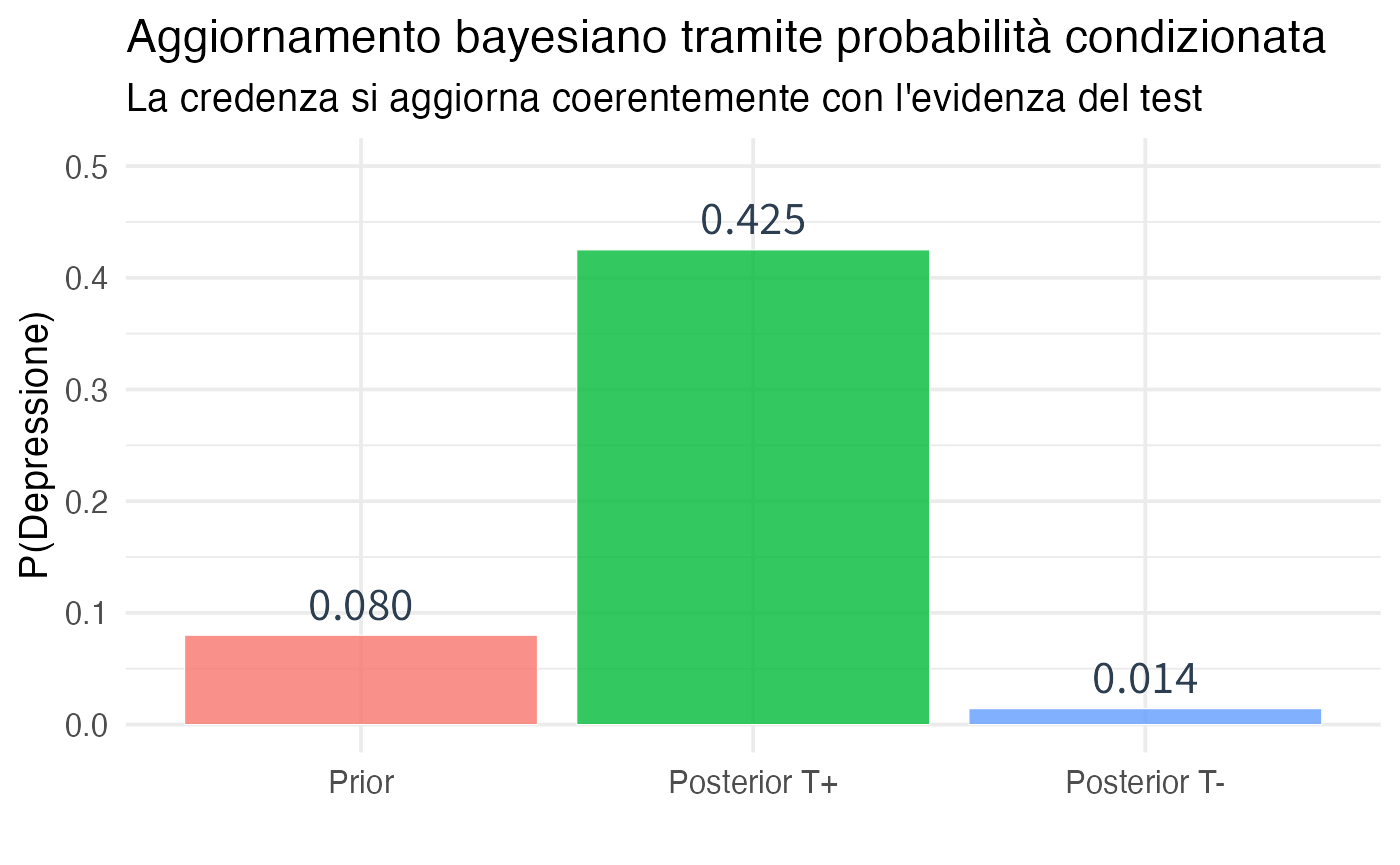
\includegraphics[width=0.85\linewidth,height=\textheight,keepaspectratio]{chapters/probability/04_conditional_prob_bayesian_files/figure-pdf/unnamed-chunk-4-1.png}

\textbf{Verifica con simulazione Monte Carlo}:

\begin{Shaded}
\begin{Highlighting}[]
\FunctionTok{set.seed}\NormalTok{(}\DecValTok{123}\NormalTok{)}
\NormalTok{N }\OtherTok{\textless{}{-}} \DecValTok{100000}

\CommentTok{\# Simulare stato reale e risultato test}
\NormalTok{stato }\OtherTok{\textless{}{-}} \FunctionTok{rbinom}\NormalTok{(N, }\DecValTok{1}\NormalTok{, P\_D)  }\CommentTok{\# 1 = Depresso, 0 = Non depresso}

\NormalTok{test\_result }\OtherTok{\textless{}{-}} \FunctionTok{ifelse}\NormalTok{(stato }\SpecialCharTok{==} \DecValTok{1}\NormalTok{,}
                      \FunctionTok{rbinom}\NormalTok{(N, }\DecValTok{1}\NormalTok{, sens),      }\CommentTok{\# Se depresso, test+ con prob sens}
                      \FunctionTok{rbinom}\NormalTok{(N, }\DecValTok{1}\NormalTok{, fp\_rate))   }\CommentTok{\# Se non depresso, test+ con prob fp\_rate}

\CommentTok{\# Calcolare condizionate empiriche}
\NormalTok{P\_D\_given\_Tpos\_sim }\OtherTok{\textless{}{-}} \FunctionTok{mean}\NormalTok{(stato[test\_result }\SpecialCharTok{==} \DecValTok{1}\NormalTok{] }\SpecialCharTok{==} \DecValTok{1}\NormalTok{)}
\NormalTok{P\_D\_given\_Tneg\_sim }\OtherTok{\textless{}{-}} \FunctionTok{mean}\NormalTok{(stato[test\_result }\SpecialCharTok{==} \DecValTok{0}\NormalTok{] }\SpecialCharTok{==} \DecValTok{1}\NormalTok{)}
\end{Highlighting}
\end{Shaded}

I risultati della simulazione confermano i calcoli analitici: -
\(P(D \mid T^+)_{sim} = 0.418\) vs.~\(P(D \mid T^+)_{teor} = 0.425\) -
\(P(D \mid T^-)_{sim} = 0.014\) vs.~\(P(D \mid T^-)_{teor} = 0.014\)

\end{tcolorbox}

\section{Indipendenza stocastica}\label{indipendenza-stocastica}

Il concetto di indipendenza rappresenta una proprietà fondamentale che
caratterizza l'assenza di relazione informativa tra eventi nell'ambito
del ragionamento probabilistico.

\begin{definition}[Indipendenza (definizione
epistemica)]\protect\hypertarget{def-independence}{}\label{def-independence}

Due eventi \(A\) e \(B\) sono \textbf{indipendenti} (notazione:
\(A \perp B\)) quando l'acquisizione di informazione riguardante uno dei
due eventi non modifica le nostre credenze relative all'altro:

\begin{equation}\phantomsection\label{eq-independence-def}{
P(A \mid B) = P(A) \quad \text{e equivalentemente} \quad P(B \mid A) = P(B).
}\end{equation}

\textbf{Conseguenza matematica}: se \(A \perp B\), allora la loro
probabilità congiunta ammette una fattorizzazione moltiplicativa:
\begin{equation}\phantomsection\label{eq-independence-prod}{
P(A \cap B) = P(A) \cdot P(B)
}\end{equation}

\textbf{Interpretazione epistemica}: l'informazione che ``\(B\) si è
verificato'' non modifica la nostra credenza riguardo al verificarsi di
\(A\). Gli eventi sono epistemicamente disgiunti: la conoscenza di uno
non fornisce alcuna informazione utile né per prevedere il verificarsi
dell'altro né per determinarne la probabilità.

\end{definition}

\subsection{Test di indipendenza nella tabella
congiunta}\label{test-di-indipendenza-nella-tabella-congiunta}

Data una distribuzione di probabilità congiunta rappresentata in forma
tabellare, è possibile verificare l'eventuale indipendenza tra due
eventi confrontando la probabilità congiunta osservata \(P(A \cap B)\)
con il prodotto delle probabilità marginali \(P(A) \cdot P(B)\). Se
queste due quantità coincidono, possiamo concludere che gli eventi sono
statisticamente indipendenti.

\begin{Shaded}
\begin{Highlighting}[]
\CommentTok{\# Esempio: Test e Stato sono indipendenti?}
\NormalTok{P\_A }\OtherTok{\textless{}{-}} \FunctionTok{rowSums}\NormalTok{(tab\_diagnostic)[}\DecValTok{1}\NormalTok{]  }\CommentTok{\# P(D)}
\NormalTok{P\_B }\OtherTok{\textless{}{-}} \FunctionTok{colSums}\NormalTok{(tab\_diagnostic)[}\DecValTok{1}\NormalTok{]  }\CommentTok{\# P(T+)}
\NormalTok{P\_AB\_obs }\OtherTok{\textless{}{-}}\NormalTok{ tab\_diagnostic[}\DecValTok{1}\NormalTok{, }\DecValTok{1}\NormalTok{]   }\CommentTok{\# P(D ∩ T+)}
\NormalTok{P\_AB\_indep }\OtherTok{\textless{}{-}}\NormalTok{ P\_A }\SpecialCharTok{*}\NormalTok{ P\_B            }\CommentTok{\# Se fossero indipendenti}
\end{Highlighting}
\end{Shaded}

Nel caso del test diagnostico per la depressione, la differenza tra la
probabilità congiunta osservata e il prodotto delle marginali è
rilevante, il che indica che gli eventi sono dipendenti. Ciò è
auspicabile e atteso: un test diagnostico efficace deve fornire
informazioni sulla condizione che intende rilevare.

\begin{tcolorbox}[enhanced jigsaw, arc=.35mm, breakable, colbacktitle=quarto-callout-warning-color!10!white, opacityback=0, toprule=.15mm, rightrule=.15mm, colback=white, opacitybacktitle=0.6, leftrule=.75mm, coltitle=black, bottomtitle=1mm, left=2mm, toptitle=1mm, title=\textcolor{quarto-callout-warning-color}{\faExclamationTriangle}\hspace{0.5em}{Errore concettuale comune}, titlerule=0mm, bottomrule=.15mm, colframe=quarto-callout-warning-color-frame]

\subsubsection*{\texorpdfstring{Indipendenza \(\neq\)
Disgiunzione}{Indipendenza \textbackslash neq Disgiunzione}}\label{indipendenza-neq-disgiunzione}

Due eventi \emph{disgiunti} (mutualmente esclusivi) non possono essere
indipendenti, a meno che uno dei due non abbia probabilità zero.

\textbf{Dimostrazione logica}: se \(A \cap B = \varnothing\) e
\(P(A), P(B) > 0\), allora \(P(A \cap B) = 0\) mentre
\(P(A) \cdot P(B) > 0\), quindi gli eventi non sono indipendenti.

\textbf{Interpretazione epistemica}: gli eventi disgiunti sono
\emph{massimamente dipendenti} dal punto di vista informativo.
L'informazione che uno si è verificato implica con certezza che l'altro
non si è verificato. La relazione informativa è completa e
deterministica, in netto contrasto con l'indipendenza che caratterizza
l'assenza completa di informazione reciproca.

\end{tcolorbox}

\begin{Shaded}
\begin{Highlighting}[]
\CommentTok{\# Esempio numerico: eventi disgiunti}
\NormalTok{P\_pari }\OtherTok{\textless{}{-}} \DecValTok{3}\SpecialCharTok{/}\DecValTok{6}
\NormalTok{P\_dispari }\OtherTok{\textless{}{-}} \DecValTok{3}\SpecialCharTok{/}\DecValTok{6}
\NormalTok{P\_pari\_e\_dispari }\OtherTok{\textless{}{-}} \DecValTok{0}  \CommentTok{\# Disgiunti!}
\end{Highlighting}
\end{Shaded}

L'esempio dei numeri pari e dispari in un lancio di dado mostra come gli
eventi disgiunti mostrino una dipendenza informativa massima: la
conoscenza che è uscito un numero pari rende impossibile l'uscita di un
numero dispari e viceversa.

\section{Teorema del prodotto (regola della
catena)}\label{teorema-del-prodotto-regola-della-catena}

Il teorema del prodotto fornisce un metodo alternativo, spesso più
intuitivo, per esprimere le probabilità congiunte attraverso una
scomposizione sequenziale.

\begin{theorem}[Teorema del
prodotto]\protect\hypertarget{thm-product-rule}{}\label{thm-product-rule}

Per due eventi \(A\) e \(B\) con \(P(B) > 0\) vale la relazione:

\begin{equation}\phantomsection\label{eq-product-rule}{
P(A \cap B) = P(A \mid B) \cdot P(B)
}\end{equation}

\textbf{Generalizzazione} a \(n\) eventi: \[
P(A_1 \cap A_2 \cap \cdots \cap A_n) = P(A_1) \cdot P(A_2 \mid A_1) \cdot P(A_3 \mid A_1 \cap A_2) \cdots P(A_n \mid A_1 \cap \cdots \cap A_{n-1}).
\]

\textbf{Interpretazione epistemica}: la costruzione della probabilità
congiunta avviene attraverso un processo sequenziale di aggiornamento
delle credenze. Si inizia con \(P(A_1)\) (credenza iniziale sul primo
evento), poi si procede con l'aggiornamento sequenziale di ogni evento
successivo alla luce degli eventi già condizionanti.

\end{theorem}

La dimostrazione della relazione fondamentale discende immediatamente
dalla definizione di probabilità condizionata, mentre la forma estesa
per \(n\) eventi si dimostra per induzione matematica.

\begin{tcolorbox}[enhanced jigsaw, arc=.35mm, breakable, colbacktitle=quarto-callout-note-color!10!white, opacityback=0, toprule=.15mm, rightrule=.15mm, colback=white, opacitybacktitle=0.6, leftrule=.75mm, coltitle=black, bottomtitle=1mm, left=2mm, toptitle=1mm, title=\textcolor{quarto-callout-note-color}{\faInfo}\hspace{0.5em}{Esempio: Test diagnostici multipli}, titlerule=0mm, bottomrule=.15mm, colframe=quarto-callout-note-color-frame]

Un paziente con sospetto disturbo d'ansia si sottopone a due test
diagnostici indipendenti: \(T_1\) (questionario autosomministrato) e
\(T_2\) (colloquio clinico strutturato).

\textbf{Informazioni cliniche disponibili}:

\begin{itemize}
\tightlist
\item
  prevalenza del disturbo: \(P(\text{Ansia}) = 0.20\);
\item
  sensibilità del questionario: \(P(T_1^+ \mid \text{Ansia}) = 0.80\);
\item
  falsi positivi del questionario:
  \(P(T_1^+ \mid \text{Ansia}^c) = 0.15\);
\item
  sensibilità del colloquio: \(P(T_2^+ \mid \text{Ansia}) = 0.85\);
\item
  falsi positivi del colloquio: \(P(T_2^+ \mid \text{Ansia}^c) = 0.10\).
\end{itemize}

I due test sono \emph{condizionatamente indipendenti} dato lo stato del
paziente.

\textbf{Applicazione del teorema del prodotto}: la probabilità che il
paziente sia effettivamente ansioso e risulti positivo ad entrambi i
test si calcola come: \[
P(\text{Ansia} \cap T_1^+ \cap T_2^+) = P(T_2^+ \mid \text{Ansia}) \cdot P(T_1^+ \mid \text{Ansia}) \cdot P(\text{Ansia}) = 0.85 \times 0.80 \times 0.20 = 0.136.
\]

\textbf{Interpretazione}: la probabilità che un paziente sia
effettivamente ansioso e risulti positivo ad entrambi i test è del
13.6\%. Questo risultato combina la probabilità a priori del disturbo
con le caratteristiche psicometriche dei due test, sfruttando la loro
indipendenza condizionale.

\end{tcolorbox}

\section{Legge della probabilità
totale}\label{legge-della-probabilituxe0-totale}

La legge della probabilità totale costituisce un'applicazione
fondamentale del teorema del prodotto in contesti in cui lo spazio
campionario risulta suddiviso in scenari mutualmente esclusivi.

\begin{theorem}[Legge della probabilità
totale]\protect\hypertarget{thm-total-probability}{}\label{thm-total-probability}

Sia \(\{B_1, B_2, \ldots, B_n\}\) una \emph{partizione} di
\(\Omega\)---ovvero una collezione di eventi mutualmente esclusivi ed
esaustivi che ricoprono l'intero spazio campionario. Allora, per ogni
evento \(A\):

\begin{equation}\phantomsection\label{eq-total-probability}{
P(A) = \sum_{i=1}^{n} P(A \mid B_i) \cdot P(B_i).
}\end{equation}

\textbf{Interpretazione epistemica}: la credenza complessiva nell'evento
\(A\) corrisponde a una media ponderata delle credenze condizionate a
ciascuno scenario \(B_i\), dove i pesi sono rappresentati dalle nostre
credenze iniziali nei diversi scenari.

\end{theorem}

\subsection{Applicazione a contesti
diagnostici}\label{applicazione-a-contesti-diagnostici}

Consideriamo uno scenario clinico che coinvolge due diverse popolazioni:
pazienti provenienti da una clinica specialistica (30\% del totale) e
soggetti della popolazione generale (70\% del totale). Le prevalenze del
disturbo differiscono significativamente tra i due gruppi: 40\% nella
popolazione clinica e 5\% in quella generale.

Applicando la legge della probabilità totale con un test caratterizzato
da sensibilità 85\% e specificità 90\%, otteniamo che la probabilità
complessiva di un test positivo risulta pari a 0.20. Questo valore
emerge come media ponderata delle probabilità condizionate ai due
scenari, dimostrando come la composizione della popolazione influenzi le
performance del test diagnostico.

La struttura ad albero evidenzia il percorso inferenziale: partendo
dalla distribuzione della popolazione tra i due scenari, si calcolano le
probabilità di test positivo in ciascun contesto, per poi combinarle
attraverso una media pesata che riflette le proporzioni relative dei
diversi sottogruppi.

\begin{verbatim}
#> 
#> Struttura ad albero:
#>               [Popolazione Totale]
#>                     /        \
#>                    /          \
#>          Clinica (0.3)    Pop.Gen. (0.7)
#>             |                  |
#>          T+ (0.36)          T+ (0.13)
#>                                |
#>                     P(T+) totale = 0.36×0.3 + 0.13×0.7 = 0.20
\end{verbatim}

\section{Paradosso di Simpson}\label{paradosso-di-simpson}

Il paradosso di Simpson rivela come una relazione osservata tra due
variabili possa \textbf{invertire direzione} quando si analizzano
separatamente i sottogruppi della popolazione. Questo fenomeno si
verifica quando una \textbf{variabile confondente} (come la gravità del
caso o caratteristiche demografiche) influenza sia l'esposizione sia
l'esito.

\begin{tcolorbox}[enhanced jigsaw, arc=.35mm, breakable, colbacktitle=quarto-callout-note-color!10!white, opacityback=0, toprule=.15mm, rightrule=.15mm, colback=white, opacitybacktitle=0.6, leftrule=.75mm, coltitle=black, bottomtitle=1mm, left=2mm, toptitle=1mm, title=\textcolor{quarto-callout-note-color}{\faInfo}\hspace{0.5em}{Esempio}, titlerule=0mm, bottomrule=.15mm, colframe=quarto-callout-note-color-frame]

\textbf{Efficacia del trattamento per la depressione in due cliniche}

Due cliniche (A e B) valutano un nuovo trattamento per la depressione.
La clinica A tratta soprattutto casi lievi, la clinica B casi gravi.

\textbf{Dati:}

\begin{Shaded}
\begin{Highlighting}[]
\CommentTok{\# Clinica A (casi lievi)}
\NormalTok{n\_A\_trattati }\OtherTok{\textless{}{-}} \DecValTok{90}
\NormalTok{n\_A\_guariti\_trattati }\OtherTok{\textless{}{-}} \DecValTok{81}   \CommentTok{\# 90\% successo}

\NormalTok{n\_A\_controllo }\OtherTok{\textless{}{-}} \DecValTok{10}
\NormalTok{n\_A\_guariti\_controllo }\OtherTok{\textless{}{-}} \DecValTok{9}   \CommentTok{\# 90\% successo}

\CommentTok{\# Clinica B (casi gravi)}
\NormalTok{n\_B\_trattati }\OtherTok{\textless{}{-}} \DecValTok{10}
\NormalTok{n\_B\_guariti\_trattati }\OtherTok{\textless{}{-}} \DecValTok{2}    \CommentTok{\# 20\% successo}

\NormalTok{n\_B\_controllo }\OtherTok{\textless{}{-}} \DecValTok{90}
\NormalTok{n\_B\_guariti\_controllo }\OtherTok{\textless{}{-}} \DecValTok{27}  \CommentTok{\# 30\% successo}

\CommentTok{\# Proporzioni per clinica}
\NormalTok{prop\_A\_trattati }\OtherTok{\textless{}{-}}\NormalTok{ n\_A\_guariti\_trattati }\SpecialCharTok{/}\NormalTok{ n\_A\_trattati}
\NormalTok{prop\_A\_controllo }\OtherTok{\textless{}{-}}\NormalTok{ n\_A\_guariti\_controllo }\SpecialCharTok{/}\NormalTok{ n\_A\_controllo}
\NormalTok{prop\_B\_trattati }\OtherTok{\textless{}{-}}\NormalTok{ n\_B\_guariti\_trattati }\SpecialCharTok{/}\NormalTok{ n\_B\_trattati}
\NormalTok{prop\_B\_controllo }\OtherTok{\textless{}{-}}\NormalTok{ n\_B\_guariti\_controllo }\SpecialCharTok{/}\NormalTok{ n\_B\_controllo}

\CommentTok{\# Aggregato (senza distinguere clinica)}
\NormalTok{n\_tot\_trattati }\OtherTok{\textless{}{-}}\NormalTok{ n\_A\_trattati }\SpecialCharTok{+}\NormalTok{ n\_B\_trattati}
\NormalTok{n\_tot\_guariti\_trattati }\OtherTok{\textless{}{-}}\NormalTok{ n\_A\_guariti\_trattati }\SpecialCharTok{+}\NormalTok{ n\_B\_guariti\_trattati}
\NormalTok{n\_tot\_controllo }\OtherTok{\textless{}{-}}\NormalTok{ n\_A\_controllo }\SpecialCharTok{+}\NormalTok{ n\_B\_controllo}
\NormalTok{n\_tot\_guariti\_controllo }\OtherTok{\textless{}{-}}\NormalTok{ n\_A\_guariti\_controllo }\SpecialCharTok{+}\NormalTok{ n\_B\_guariti\_controllo}

\NormalTok{prop\_tot\_trattati }\OtherTok{\textless{}{-}}\NormalTok{ n\_tot\_guariti\_trattati }\SpecialCharTok{/}\NormalTok{ n\_tot\_trattati}
\NormalTok{prop\_tot\_controllo }\OtherTok{\textless{}{-}}\NormalTok{ n\_tot\_guariti\_controllo }\SpecialCharTok{/}\NormalTok{ n\_tot\_controllo}
\end{Highlighting}
\end{Shaded}

\begin{verbatim}
#> === PARADOSSO DI SIMPSON ===
#> Clinica A (casi lievi):
#>   Trattati: 0.9 → 81 / 90
#>   Controllo: 0.9 → 9 / 10
#>   → Efficacia uguale o leggermente migliore nel gruppo trattamento
#> Clinica B (casi gravi):
#>   Trattati: 0.2 → 2 / 10
#>   Controllo: 0.3 → 27 / 90
#>   → Trattamento migliore anche qui
#> AGGREGATO (A + B):
#>   Trattati: 0.83 → 83 / 100
#>   Controllo: 0.36 → 36 / 100
#>   → NELL'AGGREGATO: sembra che il trattamento funzioni PEGGIO!
#> Spiegazione: la clinica B (casi gravi) contribuisce molto al gruppo trattato,
#> mentre la clinica A (casi lievi) contribuisce molto al gruppo di controllo.
#> Il mix diseguale dei casi (variabile confondente) inverte la relazione osservata.
\end{verbatim}

\textbf{Visualizzazione}

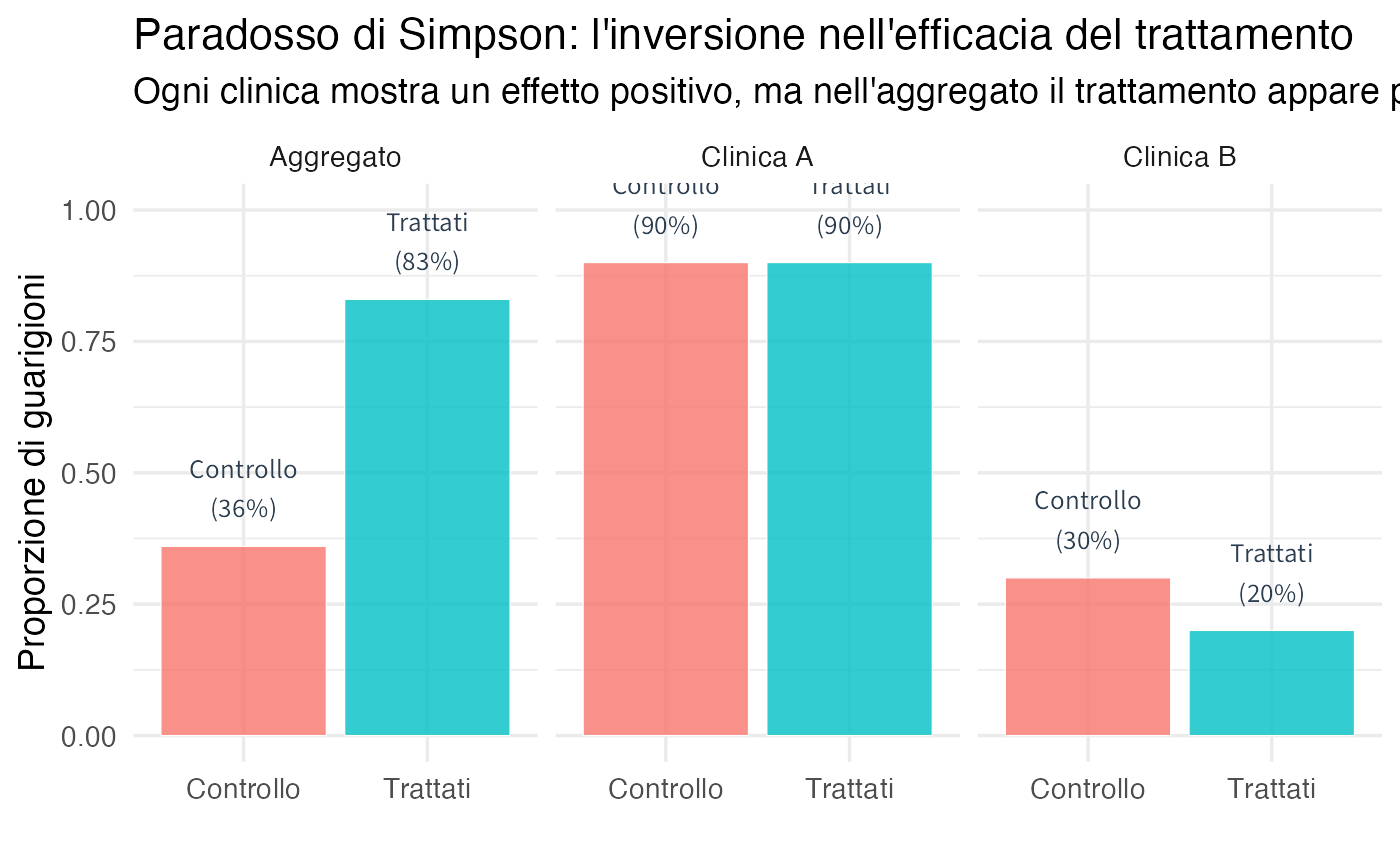
\includegraphics[width=0.85\linewidth,height=\textheight,keepaspectratio]{chapters/probability/04_conditional_prob_bayesian_files/figure-pdf/unnamed-chunk-11-1.png}

Analizzando separatamente i dati di ciascuna clinica, il trattamento
mostra un'efficacia positiva in entrambi i contesti. Tuttavia, quando i
dati vengono aggregati, emerge un risultato controintuitivo: il
trattamento appare complessivamente meno efficace del gruppo di
controllo.

Questo paradosso si spiega considerando la distribuzione diseguale dei
casi tra i gruppi: la clinica B (casi gravi) contribuisce maggiormente
al gruppo trattato, mentre la clinica A (casi lievi) prevale nel gruppo
di controllo. La variabile confondente ``gravità del caso'' distorce la
relazione osservata a livello aggregato.

\textbf{Interpretazione epistemica:} la probabilità condizionata
corretta non è quella aggregata ma quella stratificata per clinica.
L'analisi aggregata, ignorando la variabile confondente, può condurre a
conclusioni erronee nonostante il trattamento sia benefico in tutti i
sottogruppi.

\end{tcolorbox}

\section*{Riflessioni conclusive}\label{riflessioni-conclusive-3}

\markright{Riflessioni conclusive}

La probabilità condizionata rappresenta il meccanismo formale attraverso
il quale le credenze si aggiornano in modo coerente quando nuove
informazioni diventano disponibili. Questo capitolo ha esaminato i
principi fondamentali di questo meccanismo.

Dal punto di vista epistemico, l'espressione \(P(A \mid B)\) formalizza
quantitativamente il grado di fiducia in \(A\) dopo l'acquisizione
dell'informazione \(B\). Questo aggiornamento si realizza attraverso un
processo di contrazione e rinormalizzazione dello spazio delle
possibilità. Il concetto di indipendenza probabilistica, al contrario,
caratterizza le situazioni in cui gli eventi non forniscono informazioni
reciproche: la conoscenza di uno non altera la probabilità assegnata
all'altro.

Il teorema del prodotto fornisce la regola per costruire distribuzioni
congiunte a partire da probabilità condizionate sequenziali, mentre la
legge della probabilità totale permette di scomporre le probabilità
marginali in medie ponderate delle probabilità condizionate. Il
paradosso di Simpson evidenzia la necessità di condizionare su variabili
rilevanti, mostrando come aggregazioni non appropriate possano invertire
artificialmente le relazioni causali sottostanti.

La probabilità condizionata rappresenta quindi non solo uno strumento
tecnico, ma anche il fondamento concettuale del pensiero bayesiano. Nel
prossimo capitolo, il teorema di Bayes emergerà come caso particolare di
probabilità condizionata che formalizza l'inversione probabilistica e
che permette di passare da \(P(\text{Evidenza} \mid \text{Ipotesi})\) a
\(P(\text{Ipotesi} \mid \text{Evidenza})\).

Ogni volta che utilizziamo espressioni come ``dato che'', ``sapendo
che'' o ``alla luce di'', stiamo implicitamente applicando il principio
della probabilità condizionata per aggiornare le nostre credenze in modo
logicamente strutturato e matematicamente rigoroso.

\section*{Esercizi}\label{esercizi-1}
\addcontentsline{toc}{section}{Esercizi}

\markright{Esercizi}

\begin{tcolorbox}[enhanced jigsaw, arc=.35mm, breakable, colbacktitle=quarto-callout-important-color!10!white, opacityback=0, toprule=.15mm, rightrule=.15mm, colback=white, opacitybacktitle=0.6, leftrule=.75mm, coltitle=black, bottomtitle=1mm, left=2mm, toptitle=1mm, title=\textcolor{quarto-callout-important-color}{\faExclamation}\hspace{0.5em}{Problemi}, titlerule=0mm, bottomrule=.15mm, colframe=quarto-callout-important-color-frame]

\subsection{Esercizi concettuali}\label{esercizi-concettuali}

\begin{enumerate}
\def\labelenumi{\arabic{enumi}.}
\item
  Spiega perché ``ogni probabilità è condizionata'' da una prospettiva
  bayesiana. Cosa significa \(P(A)\) implicitamente?
\item
  La formula \(P(A \mid B) = P(A \cap B) / P(B)\) può sembrare
  circolare. Spiega perché non lo è, e in quale ordine concettuale
  pensiamo queste quantità.
\item
  Quando due eventi sono disgiunti, possono essere indipendenti? Perché
  o perché no?
\item
  Il teorema del prodotto dice \(P(A \cap B) = P(A \mid B) P(B)\).
  Questo è simmetrico? Cioè, posso scrivere
  \(P(A \cap B) = P(B \mid A) P(A)\)? Cosa implica questa simmetria?
\item
  Il paradosso di Simpson dimostra che l'aggregazione è sempre
  sbagliata? Quando è legittimo aggregare dati?
\end{enumerate}

\subsection{Esercizi su probabilità
condizionata}\label{esercizi-su-probabilituxe0-condizionata}

\begin{enumerate}
\def\labelenumi{\arabic{enumi}.}
\setcounter{enumi}{5}
\item
  Data una tabella congiunta: \textbar{} \textbar{} \(B\) \textbar{}
  \(B^c\) \textbar{}
  \textbar-------\textbar------\textbar-------\textbar{} \textbar{}
  \(A\) \textbar{} 0.20 \textbar{} 0.30 \textbar{} \textbar{} \(A^c\)
  \textbar{} 0.15 \textbar{} 0.35 \textbar{}

  Calcola:

  \begin{enumerate}
  \def\labelenumii{\alph{enumii}.}
  \tightlist
  \item
    \(P(A \mid B)\)
  \item
    \(P(B \mid A)\)
  \item
    \(P(A \mid B^c)\)
  \item
    Gli eventi sono indipendenti?
  \end{enumerate}
\item
  \(P(A) = 0.6\), \(P(B) = 0.5\), \(P(A \mid B) = 0.7\). Calcola:

  \begin{enumerate}
  \def\labelenumii{\alph{enumii}.}
  \tightlist
  \item
    \(P(A \cap B)\)
  \item
    \(P(B \mid A)\)
  \item
    \(P(A \cup B)\)
  \end{enumerate}
\item
  Test diagnostico: \(P(M) = 0.01\), sens = 0.95, spec = 0.98.

  \begin{enumerate}
  \def\labelenumii{\alph{enumii}.}
  \tightlist
  \item
    Costruisci tabella congiunta
  \item
    Calcola VPP e VPN
  \item
    Quanto deve essere alta la sensibilità per avere VPP \textgreater{}
    0.9?
  \end{enumerate}
\end{enumerate}

\subsection{Esercizi su indipendenza}\label{esercizi-su-indipendenza}

\begin{enumerate}
\def\labelenumi{\arabic{enumi}.}
\setcounter{enumi}{8}
\tightlist
\item
  Un dado viene lanciato. Siano:

  \begin{itemize}
  \tightlist
  \item
    \(A\) = ``Esce numero pari''
  \item
    \(B\) = ``Esce numero ≤ 3''
  \end{itemize}

  \begin{enumerate}
  \def\labelenumii{\alph{enumii}.}
  \tightlist
  \item
    \(A\) e \(B\) sono indipendenti?
  \item
    Calcola \(P(A \mid B)\) e confronta con \(P(A)\)
  \end{enumerate}
\item
  Due monete equilibrate vengono lanciate. Siano:

  \begin{itemize}
  \tightlist
  \item
    \(A\) = ``Prima moneta è testa''
  \item
    \(B\) = ``Almeno una testa''
  \end{itemize}

  \begin{enumerate}
  \def\labelenumii{\alph{enumii}.}
  \tightlist
  \item
    Costruisci tabella congiunta
  \item
    Calcola \(P(A \mid B)\)
  \item
    \(A\) e \(B\) sono indipendenti?
  \end{enumerate}
\item
  In una popolazione, \(P(\text{Depressione}) = 0.15\) e
  \(P(\text{Insonnia}) = 0.25\). Se fossero indipendenti, quanto sarebbe
  \(P(\text{Depressione} \cap \text{Insonnia})\)? È plausibile
  l'indipendenza?
\end{enumerate}

\subsection{Esercizi su teorema del
prodotto}\label{esercizi-su-teorema-del-prodotto}

\begin{enumerate}
\def\labelenumi{\arabic{enumi}.}
\setcounter{enumi}{11}
\item
  \(P(A) = 0.5\), \(P(B \mid A) = 0.6\), \(P(C \mid A \cap B) = 0.7\).
  Calcola \(P(A \cap B \cap C)\).
\item
  Tre test sequenziali per ansia, ciascuno con sens = 0.80 (indipendenti
  dato stato). \(P(\text{Ansia}) = 0.20\). Calcola
  \(P(\text{Ansia} \cap T_1^+ \cap T_2^+ \cap T_3^+)\).
\item
  Usa la regola del prodotto per dimostrare che se \(A\) e \(B\) sono
  indipendenti, allora \(A\) e \(B^c\) sono indipendenti.
\end{enumerate}

\subsection{Esercizi su probabilità
totale}\label{esercizi-su-probabilituxe0-totale}

\begin{enumerate}
\def\labelenumi{\arabic{enumi}.}
\setcounter{enumi}{14}
\item
  Una clinica riceve pazienti da due fonti:

  \begin{itemize}
  \tightlist
  \item
    60\% da medico di base (prevalenza depressione = 10\%)
  \item
    40\% da pronto soccorso (prevalenza depressione = 30\%)
  \end{itemize}

  Qual è la prevalenza complessiva nella clinica?
\item
  Un questionario ha due versioni (A e B), distribuite casualmente (50\%
  ciascuna). La versione A è più facile:

  \begin{itemize}
  \tightlist
  \item
    \(P(\text{punteggio} > 20 \mid \text{Versione A}) = 0.7\)
  \item
    \(P(\text{punteggio} > 20 \mid \text{Versione B}) = 0.4\)
  \end{itemize}

  Qual è \(P(\text{punteggio} > 20)\) complessivamente?
\item
  Dimostra che \(P(A) = P(A \mid B) P(B) + P(A \mid B^c) P(B^c)\) usando
  la legge della probabilità totale con partizione \(\{B, B^c\}\).
\end{enumerate}

\subsection{Esercizi su Paradosso di
Simpson}\label{esercizi-su-paradosso-di-simpson}

\begin{enumerate}
\def\labelenumi{\arabic{enumi}.}
\setcounter{enumi}{17}
\item
  Considera questi dati su un farmaco antidepressivo:

  \textbf{Pazienti giovani} (N=200):

  \begin{itemize}
  \tightlist
  \item
    Farmaco: 70/100 migliorati (70\%)
  \item
    Placebo: 50/100 migliorati (50\%)
  \end{itemize}

  \textbf{Pazienti anziani} (N=200):

  \begin{itemize}
  \tightlist
  \item
    Farmaco: 60/100 migliorati (60\%)
  \item
    Placebo: 40/100 migliorati (40\%)
  \end{itemize}

  \begin{enumerate}
  \def\labelenumii{\alph{enumii}.}
  \tightlist
  \item
    In ciascun gruppo, il farmaco è migliore?
  \item
    Calcola le proporzioni aggregate (tutti i pazienti insieme)
  \item
    Costruisci uno scenario dove l'aggregato inverte la tendenza
  \end{enumerate}
\item
  Spiega in termini epistemici perché il paradosso di Simpson non è
  veramente un ``paradosso'' ma un avvertimento sull'importanza di
  condizionare correttamente.
\end{enumerate}

\subsection{Esercizi applicati
(psicologia)}\label{esercizi-applicati-psicologia-1}

\begin{enumerate}
\def\labelenumi{\arabic{enumi}.}
\setcounter{enumi}{19}
\tightlist
\item
  \textbf{Test per disturbo d'ansia sociale}:

  \begin{itemize}
  \tightlist
  \item
    Prevalenza in popolazione universitaria: 5\%
  \item
    Sensibilità: 85\%
  \item
    Specificità: 92\%
  \end{itemize}

  \begin{enumerate}
  \def\labelenumii{\alph{enumii}.}
  \tightlist
  \item
    Costruisci tabella congiunta completa
  \item
    Uno studente risulta positivo. Qual è la probabilità che abbia
    davvero il disturbo?
  \item
    Quale prevalenza minima serve per avere VPP \textgreater{} 0.5?
  \end{enumerate}
\item
  \textbf{Comorbidità PTSD e Depressione}:

  \begin{itemize}
  \tightlist
  \item
    In un campione clinico: \(P(\text{PTSD}) = 0.30\),
    \(P(\text{Depressione}) = 0.45\)
  \item
    Osservi che \(P(\text{Depressione} \mid \text{PTSD}) = 0.70\)
  \end{itemize}

  \begin{enumerate}
  \def\labelenumii{\alph{enumii}.}
  \tightlist
  \item
    Calcola \(P(\text{PTSD} \cap \text{Depressione})\)
  \item
    Calcola \(P(\text{PTSD} \mid \text{Depressione})\)
  \item
    Sono indipendenti? Commenta il risultato clinicamente
  \end{enumerate}
\item
  \textbf{Due test per ADHD in un bambino}:

  \begin{itemize}
  \tightlist
  \item
    Prior: \(P(\text{ADHD}) = 0.08\) (popolazione generale)
  \item
    Test comportamentale: positivo (sens=0.80, spec=0.90)
  \item
    Test cognitivo: positivo (sens=0.75, spec=0.85)
  \item
    Assumendo indipendenza condizionale:
  \end{itemize}

  \begin{enumerate}
  \def\labelenumii{\alph{enumii}.}
  \tightlist
  \item
    Calcola \(P(\text{ADHD} \mid T_1^+)\) dopo primo test
  \item
    Calcola \(P(\text{ADHD} \mid T_1^+, T_2^+)\) dopo entrambi i test
  \item
    Visualizza l'aggiornamento sequenziale delle credenze
  \end{enumerate}
\end{enumerate}

\subsection{Esercizi computazionali}\label{esercizi-computazionali-1}

\begin{enumerate}
\def\labelenumi{\arabic{enumi}.}
\setcounter{enumi}{22}
\tightlist
\item
  Scrivi una funzione R che:

  \begin{itemize}
  \tightlist
  \item
    Input: tabella congiunta 2×2
  \item
    Output: tutte le probabilità condizionate possibili e test di
    indipendenza
  \end{itemize}
\item
  Simula il paradosso di Simpson:

  \begin{itemize}
  \tightlist
  \item
    Genera dati per due gruppi con trend positivo in ciascuno
  \item
    Aggrega i dati mostrando inversione del trend
  \item
    Visualizza con ggplot
  \end{itemize}
\item
  Crea una visualizzazione interattiva (o animazione) che mostra come
  \(P(A \mid B)\) varia al variare della ``forza'' dell'associazione tra
  \(A\) e \(B\) (da indipendenza a dipendenza totale).
\end{enumerate}

\end{tcolorbox}

\begin{tcolorbox}[enhanced jigsaw, arc=.35mm, breakable, colbacktitle=quarto-callout-tip-color!10!white, opacityback=0, toprule=.15mm, rightrule=.15mm, colback=white, opacitybacktitle=0.6, leftrule=.75mm, coltitle=black, bottomtitle=1mm, left=2mm, toptitle=1mm, title=\textcolor{quarto-callout-tip-color}{\faLightbulb}\hspace{0.5em}{Soluzioni selezionate}, titlerule=0mm, bottomrule=.15mm, colframe=quarto-callout-tip-color-frame]

\subsection{Soluzioni esercizi
concettuali}\label{soluzioni-esercizi-concettuali}

\begin{enumerate}
\def\labelenumi{\arabic{enumi}.}
\item
  Da prospettiva bayesiana, ogni probabilità riflette uno stato di
  informazione. Scrivere \(P(A)\) è abbreviazione per
  \(P(A \mid \mathcal{I})\) dove \(\mathcal{I}\) è ``tutto ciò che
  sappiamo''. Non esistono probabilità ``incondizionate''---solo
  probabilità condizionate allo sfondo informativo corrente.
\item
  Non è circolare perché concettualmente partiamo dalla \textbf{tabella
  congiunta} \(P(A \cap B)\) (rappresentazione completa del nostro stato
  di credenza), poi \textbf{deriviamo} le condizionate come rapporti. La
  formula ci dice \emph{come calcolare} condizionate da congiunte, non
  \emph{come definire} le congiunte.
\item
  No (a meno che uno abbia probabilità zero). Eventi disgiunti hanno
  informazione reciproca \textbf{massima}: sapere che uno è vero implica
  certezza che l'altro è falso. Indipendenza richiede \emph{assenza} di
  informazione.
\item
  Sì, è simmetrico:
  \(P(A \cap B) = P(A \mid B) P(B) = P(B \mid A) P(A)\). Questa
  simmetria è il cuore del teorema di Bayes! Mostra che la congiunta può
  essere costruita in due modi equivalenti.
\item
  No, l'aggregazione è legittima quando non c'è confondente rilevante, o
  quando la confondente è distribuita uniformemente. Il paradosso
  avverte: \emph{esplicita le tue assunzioni di omogeneità prima di
  aggregare}.
\end{enumerate}

\subsection{Soluzioni probabilità
condizionata}\label{soluzioni-probabilituxe0-condizionata}

\begin{enumerate}
\def\labelenumi{\arabic{enumi}.}
\setcounter{enumi}{5}
\tightlist
\item
  \begin{enumerate}
  \def\labelenumii{\alph{enumii}.}
  \tightlist
  \item
    \(P(A \mid B) = 0.20 / (0.20 + 0.15) = 0.571\)
  \item
    \(P(B \mid A) = 0.20 / (0.20 + 0.30) = 0.400\)
  \item
    \(P(A \mid B^c) = 0.30 / (0.30 + 0.35) = 0.462\)
  \item
    Test: \(P(A) = 0.50\), \(P(B) = 0.35\),
    \(P(A) P(B) = 0.175 \neq P(A \cap B) = 0.20\). NON indipendenti.
  \end{enumerate}
\item
  \begin{enumerate}
  \def\labelenumii{\alph{enumii}.}
  \tightlist
  \item
    \(P(A \cap B) = P(A \mid B) P(B) = 0.7 \times 0.5 = 0.35\)
  \item
    \(P(B \mid A) = P(A \cap B) / P(A) = 0.35 / 0.6 \approx 0.583\)
  \item
    \(P(A \cup B) = 0.6 + 0.5 - 0.35 = 0.75\)
  \end{enumerate}
\item
  \begin{enumerate}
  \def\labelenumii{\alph{enumii}.}
  \tightlist
  \item
    Tabella: \(P(M \cap T^+) = 0.0095\), \(P(M \cap T^-) = 0.0005\),
    etc.
  \item
    VPP = \(0.0095 / (0.0095 + 0.0198) \approx 0.324\); VPN
    \(\approx 0.9995\)
  \item
    Per VPP \textgreater{} 0.9: serve sens \(\approx 0.998\) (quasi
    perfetta con prevalenza così bassa!)
  \end{enumerate}
\end{enumerate}

\subsection{Soluzioni indipendenza}\label{soluzioni-indipendenza}

\begin{enumerate}
\def\labelenumi{\arabic{enumi}.}
\setcounter{enumi}{8}
\tightlist
\item
  \begin{enumerate}
  \def\labelenumii{\alph{enumii}.}
  \tightlist
  \item
    \(P(A) = 1/2\), \(P(B) = 1/2\), \(P(A \cap B) = P(\{2\}) = 1/6\)
    \(P(A) P(B) = 1/4 \neq 1/6\). NON indipendenti.
  \item
    \(P(A \mid B) = (1/6) / (1/2) = 1/3 \neq 1/2 = P(A)\)
  \end{enumerate}
\item
  Spazio: \{TT, TC, CT, CC\}, equiprobabili.

  \begin{enumerate}
  \def\labelenumii{\alph{enumii}.}
  \tightlist
  \item
    Tabella con \(A\) = \{TT, TC\}, \(B\) = \{TT, TC, CT\}
  \item
    \(P(A \mid B) = P(\{TT, TC\}) / P(B) = (1/2) / (3/4) = 2/3\)
  \item
    \(P(A) = 1/2 \neq 2/3 = P(A \mid B)\). NON indipendenti.
  \end{enumerate}
\item
  Se indipendenti: \(P(D \cap I) = 0.15 \times 0.25 = 0.0375\). Ma
  clinicamente sappiamo che depressione e insonnia sono altamente
  correlate, quindi l'indipendenza è \textbf{implausibile}.
\end{enumerate}

\subsection{Soluzioni teorema del
prodotto}\label{soluzioni-teorema-del-prodotto}

\begin{enumerate}
\def\labelenumi{\arabic{enumi}.}
\setcounter{enumi}{11}
\item
  \(P(A \cap B \cap C) = P(C \mid A \cap B) \cdot P(B \mid A) \cdot P(A) = 0.7 \times 0.6 \times 0.5 = 0.21\)
\item
  \(P(\text{Ansia} \cap \text{tutti +}) = 0.80^3 \times 0.20 = 0.512 \times 0.20 = 0.1024\)
\item
  Dimostrazione:
  \texttt{P(A\ ∩\ B\^{}c)\ =\ P(A)\ -\ P(A\ ∩\ B)\ \ \ \ {[}additività{]}\ \ \ \ \ \ \ \ \ \ \ \ \ \ \ \ =\ P(A)\ -\ P(A)P(B)\ \ \ \ \ {[}indipendenza\ A,B{]}\ \ \ \ \ \ \ \ \ \ \ \ \ \ \ \ =\ P(A)(1\ -\ P(B))\ \ \ \ \ \ \ \ \ \ \ \ \ \ \ \ =\ P(A)P(B\^{}c)\ \ \ \ \ \ \ \ \ \ {[}quindi\ A\ ⊥\ B\^{}c{]}}
\end{enumerate}

\subsection{Soluzioni probabilità
totale}\label{soluzioni-probabilituxe0-totale}

\begin{enumerate}
\def\labelenumi{\arabic{enumi}.}
\setcounter{enumi}{14}
\item
  \(P(D) = 0.10 \times 0.60 + 0.30 \times 0.40 = 0.06 + 0.12 = 0.18\)
  (18\%)
\item
  \(P(>20) = 0.7 \times 0.5 + 0.4 \times 0.5 = 0.35 + 0.20 = 0.55\)
\item
  Partizione: \(B\) e \(B^c\) coprono \(\Omega\) e sono disgiunti.
  \(P(A) = P(A \cap \Omega) = P(A \cap (B \cup B^c)) = P((A \cap B) \cup (A \cap B^c))\)
  \(= P(A \cap B) + P(A \cap B^c)\) {[}disgiunzione{]}
  \(= P(A \mid B) P(B) + P(A \mid B^c) P(B^c)\) {[}def. condizionata{]}
\end{enumerate}

\subsection{Soluzioni applicazioni
psicologiche}\label{soluzioni-applicazioni-psicologiche}

\begin{enumerate}
\def\labelenumi{\arabic{enumi}.}
\setcounter{enumi}{19}
\tightlist
\item
  \begin{enumerate}
  \def\labelenumii{\alph{enumii}.}
  \tightlist
  \item
    \(P(A \cap T^+) = 0.85 \times 0.05 = 0.0425\), etc.
  \item
    VPP = \(0.0425 / (0.0425 + 0.076) = 0.359\) (solo 36\%!)
  \item
    Per VPP \textgreater{} 0.5, serve prev \(\geq 0.10\) (10\%)
  \end{enumerate}
\item
  \begin{enumerate}
  \def\labelenumii{\alph{enumii}.}
  \tightlist
  \item
    \(P(P \cap D) = P(D \mid P) \times P(P) = 0.70 \times 0.30 = 0.21\)
  \item
    \(P(P \mid D) = 0.21 / 0.45 \approx 0.467\)
  \item
    Se indipendenti: \(P(P) P(D) = 0.30 \times 0.45 = 0.135 \neq 0.21\).
    DIPENDENTI (comorbidità alta, clinicamente attesa)
  \end{enumerate}
\item
  Soluzione completa richiede costruzione sequenziale. Sketch:

  \begin{itemize}
  \tightlist
  \item
    Dopo \(T_1^+\): \(P(\text{ADHD} \mid T_1^+) \approx 0.38\)
  \item
    Dopo \(T_1^+, T_2^+\):
    \(P(\text{ADHD} \mid \text{entrambi}) \approx 0.69\)
  \item
    Visualizzazione: barplot con credenze 0.08 → 0.38 → 0.69
  \end{itemize}
\end{enumerate}

\end{tcolorbox}

\chapter{Il teorema di Bayes}\label{sec-prob-bayes-theorem}

\section*{Introduzione}\label{introduzione-5}

\markright{Introduzione}

Il teorema di Bayes costituisce il punto di arrivo naturale del percorso
concettuale sviluppato nei capitoli precedenti. Dopo aver definito la
probabilità come grado di credenza razionale
(Chapter~\ref{sec-prob-interpretation}), stabilito gli assiomi come
vincoli di coerenza (Chapter~\ref{sec-prob-axioms-coherence}),
riconosciuto l'equiprobabilità come caso particolare della simmetria
epistemica (Chapter~\ref{sec-equiprobability-combinatorics}) e
identificato la probabilità condizionata come meccanismo di
aggiornamento delle credenze (Chapter~\ref{sec-prob-conditional-prob}),
il teorema di Bayes emerge come la formalizzazione matematica di ciò che
significa \emph{apprendere dall'esperienza}.

Il teorema risolve un problema epistemologico fondamentale: come
trasformare l'informazione che dal mondo giunge a noi, sotto forma di
dati osservati, evidenze empiriche o sintomi clinici, in conoscenza
riguardante ciò che non possiamo osservare direttamente, ovvero le
cause, le ipotesi, i parametri sottostanti. Questa inversione della
direzione del condizionamento probabilistico costituisce l'essenza
dell'inferenza induttiva.

In questo capitolo esamineremo il teorema non soltanto come strumento
tecnico di calcolo, ma come principio normativo che prescrive il modo
ottimale di integrare la conoscenza pregressa con le nuove osservazioni.
Vedremo come questo meccanismo si applichi naturalmente ai problemi
diagnostici in psicologia clinica, alla valutazione delle ipotesi nella
ricerca sperimentale e al ragionamento quotidiano in condizioni di
incertezza.

\subsection*{Panoramica del capitolo}\label{panoramica-del-capitolo-4}

\begin{itemize}
\tightlist
\item
  Derivazione del teorema dalla simmetria della probabilità congiunta.
\item
  Interpretazione epistemica delle componenti: prior, likelihood,
  posterior.
\item
  Probabilità inversa come problema fondamentale dell'inferenza.
\item
  Forma in odds e rapporti di verosimiglianza per applicazioni cliniche.
\item
  Applicazioni a test diagnostici e valutazione della comorbilità.
\item
  Fallacia del tasso base e sue implicazioni per il ragionamento
  clinico.
\item
  Aggiornamento bayesiano con distribuzioni Beta.
\item
  Intervalli di credibilità e loro interpretazione epistemica.
\end{itemize}

\begin{tcolorbox}[enhanced jigsaw, arc=.35mm, breakable, colbacktitle=quarto-callout-tip-color!10!white, opacityback=0, toprule=.15mm, rightrule=.15mm, colback=white, opacitybacktitle=0.6, leftrule=.75mm, coltitle=black, bottomtitle=1mm, left=2mm, toptitle=1mm, title=\textcolor{quarto-callout-tip-color}{\faLightbulb}\hspace{0.5em}{Prerequisiti}, titlerule=0mm, bottomrule=.15mm, colframe=quarto-callout-tip-color-frame]

\begin{itemize}
\tightlist
\item
  Aver letto i capitoli precedenti, specialmente
  Chapter~\ref{sec-prob-conditional-prob}.
\item
  Leggere \emph{Everything is Predictable: How Bayesian Statistics
  Explain Our World} (\citeproc{ref-chivers2024everything}{Chivers,
  2024}).
\end{itemize}

\end{tcolorbox}

\begin{tcolorbox}[enhanced jigsaw, arc=.35mm, breakable, colbacktitle=quarto-callout-caution-color!10!white, opacityback=0, toprule=.15mm, rightrule=.15mm, colback=white, opacitybacktitle=0.6, leftrule=.75mm, coltitle=black, bottomtitle=1mm, left=2mm, toptitle=1mm, title=\textcolor{quarto-callout-caution-color}{\faFire}\hspace{0.5em}{Preparazione del Notebook}, titlerule=0mm, bottomrule=.15mm, colframe=quarto-callout-caution-color-frame]

\begin{Shaded}
\begin{Highlighting}[]
\NormalTok{here}\SpecialCharTok{::}\FunctionTok{here}\NormalTok{(}\StringTok{"code"}\NormalTok{, }\StringTok{"\_common.R"}\NormalTok{) }\SpecialCharTok{|\textgreater{}} 
  \FunctionTok{source}\NormalTok{()}

\CommentTok{\# Caricamento dei pacchetti necessari}
\ControlFlowTok{if}\NormalTok{ (}\SpecialCharTok{!}\FunctionTok{requireNamespace}\NormalTok{(}\StringTok{"pacman"}\NormalTok{)) }\FunctionTok{install.packages}\NormalTok{(}\StringTok{"pacman"}\NormalTok{)}
\NormalTok{pacman}\SpecialCharTok{::}\FunctionTok{p\_load}\NormalTok{(ggplot2, dplyr, tidyr, patchwork)}
\end{Highlighting}
\end{Shaded}

\end{tcolorbox}

\section{La simmetria fondamentale della probabilità
congiunta}\label{la-simmetria-fondamentale-della-probabilituxe0-congiunta}

Il teorema di Bayes non introduce nuovi principi, ma emerge come
conseguenza algebrica della definizione di probabilità condizionata.
Questa derivazione dimostra che l'aggiornamento bayesiano delle credenze
non costituisce una scelta arbitraria, ma rappresenta piuttosto una
necessità logica per chiunque accetti il quadro assiomatico della teoria
della probabilità.

\subsection{Dalla probabilità congiunta al teorema di
Bayes}\label{dalla-probabilituxe0-congiunta-al-teorema-di-bayes}

Nel Chapter~\ref{sec-prob-conditional-prob} abbiamo visto che la
probabilità congiunta di due eventi può essere espressa in due modi
equivalenti, a seconda di quale evento scegliamo come ``base'' per il
condizionamento:

\begin{equation}\phantomsection\label{eq-joint-symmetry}{
P(A \cap B) = P(A \mid B) \cdot P(B) = P(B \mid A) \cdot P(A).
}\end{equation}

Questa simmetria non è accidentale: riflette il fatto che la probabilità
congiunta rappresenta una struttura di credenze completa e coerente,
dalla quale possiamo estrarre diverse probabilità condizionate a seconda
della prospettiva adottata. Quando uguagliamo le due espressioni e
risolviamo per \(P(A \mid B)\), otteniamo:

\begin{theorem}[Teorema di Bayes (forma
fondamentale)]\protect\hypertarget{thm-bayes-theorem}{}\label{thm-bayes-theorem}

Per eventi \(A\) e \(B\) con \(P(B) > 0\):

\begin{equation}\phantomsection\label{eq-bayes-basic}{
P(A \mid B) = \frac{P(B \mid A) \cdot P(A)}{P(B)}.
}\end{equation}

\end{theorem}

Ciascun termine di questa espressione possiede un significato epistemico
preciso che conviene esplicitare.

La \textbf{distribuzione a priori} \(P(A)\) rappresenta il grado di
credenza iniziale nell'ipotesi \(A\) prima di considerare l'evidenza
\(B\). Questa valutazione preliminare incorpora tutto ciò che
sappiamo---o crediamo di sapere---sulla base della conoscenza pregressa:
studi precedenti, esperienza clinica, prevalenze epidemiologiche,
oppure, in condizioni di massima ignoranza, il principio di
indifferenza.

La \textbf{funzione di verosimiglianza} \(P(B \mid A)\) quantifica
quanto l'evidenza osservata sia compatibile con l'ipotesi in esame.
Questa quantità misura la capacità predittiva dell'ipotesi: se \(A\)
fosse vera, quanto sarebbe plausibile osservare proprio l'evidenza
\(B\)? Nei contesti diagnostici, questa corrisponde alla sensibilità di
un test.

L'\textbf{evidenza marginale} \(P(B)\) rappresenta la probabilità
complessiva di osservare \(B\), calcolata come media pesata su tutte le
possibili ipotesi. Questa quantità funge da costante di normalizzazione
che garantisce la coerenza probabilistica del risultato.

La \textbf{distribuzione a posteriori} \(P(A \mid B)\) esprime la
credenza rivista nell'ipotesi \(A\) dopo aver osservato l'evidenza
\(B\). Questa è la risposta alla domanda inferenziale di interesse
pratico.

Una forma spesso più illuminante nelle applicazioni è la
\textbf{versione proporzionale}: \[
P(A \mid B) \propto P(B \mid A) \cdot P(A),
\] che enfatizza come la distribuzione a posteriori sia il prodotto
ponderato di verosimiglianza e prior, con il denominatore che serve
esclusivamente a garantire la normalizzazione.

\subsection{Interpretazione attraverso le tabelle di probabilità
congiunta}\label{interpretazione-attraverso-le-tabelle-di-probabilituxe0-congiunta}

Il significato operativo del teorema diventa trasparente quando lo
esaminiamo attraverso le tabelle 2×2 introdotte nei capitoli precedenti:

\begin{longtable}[]{@{}llll@{}}
\toprule\noalign{}
& \(B\) & \(B^c\) & Marginali \\
\midrule\noalign{}
\endhead
\bottomrule\noalign{}
\endlastfoot
\(A\) & \(P(A \cap B)\) & \(P(A \cap B^c)\) & \(P(A)\) \\
\(A^c\) & \(P(A^c \cap B)\) & \(P(A^c \cap B^c)\) & \(P(A^c)\) \\
\textbf{Marginali} & \(P(B)\) & \(P(B^c)\) & \(1\) \\
\end{longtable}

In questa rappresentazione, le componenti del teorema assumono
un'interpretazione geometrica immediata. La distribuzione a priori
\(P(A)\) corrisponde alla marginale della riga associata ad \(A\). La
funzione di verosimiglianza \(P(B \mid A) = P(A \cap B) / P(A)\)
rappresenta la proporzione della riga di \(A\) che cade nella colonna di
\(B\). La distribuzione a posteriori
\(P(A \mid B) = P(A \cap B) / P(B)\) costituisce la proporzione della
colonna di \(B\) appartenente alla riga di \(A\).

Il teorema di Bayes opera dunque una \textbf{rotazione della
prospettiva}: dalla visione per righe (condizionata all'ipotesi) alla
visione per colonne (condizionata all'evidenza), sfruttando la struttura
simmetrica della distribuzione congiunta.

\subsubsection{Costruzione di una tabella di probabilità congiunta per
un test
diagnostico}\label{costruzione-di-una-tabella-di-probabilituxe0-congiunta-per-un-test-diagnostico}

Consideriamo un test per la depressione con sensibilità
\(P(T+ \mid D)=0.85\), tasso di falsi positivi \(P(T+ \mid D^c)=0.10\) e
una prevalenza della depressione pari a \(P(D)=0.15\). Da questi valori
possiamo costruire la distribuzione congiunta dei due eventi: stato
clinico (\(D\) / \(D^c\)) ed esito del test (\(T+\) / \(T-\)).

\begin{Shaded}
\begin{Highlighting}[]
\NormalTok{P\_D }\OtherTok{\textless{}{-}} \FloatTok{0.15}        \CommentTok{\# Prevalenza della depressione}
\NormalTok{sens }\OtherTok{\textless{}{-}} \FloatTok{0.85}       \CommentTok{\# Sensibilità: P(T+|D)}
\NormalTok{fp\_rate }\OtherTok{\textless{}{-}} \FloatTok{0.10}    \CommentTok{\# Tasso di falsi positivi: P(T+|D\^{}c)}
\end{Highlighting}
\end{Shaded}

\begin{Shaded}
\begin{Highlighting}[]
\CommentTok{\# Probabilità congiunte ricavate da prior e condizionate}
\NormalTok{P\_D\_and\_Tpos  }\OtherTok{\textless{}{-}}\NormalTok{ sens }\SpecialCharTok{*}\NormalTok{ P\_D}
\NormalTok{P\_D\_and\_Tneg  }\OtherTok{\textless{}{-}}\NormalTok{ (}\DecValTok{1} \SpecialCharTok{{-}}\NormalTok{ sens) }\SpecialCharTok{*}\NormalTok{ P\_D}
\NormalTok{P\_Dc\_and\_Tpos }\OtherTok{\textless{}{-}}\NormalTok{ fp\_rate }\SpecialCharTok{*}\NormalTok{ (}\DecValTok{1} \SpecialCharTok{{-}}\NormalTok{ P\_D)}
\NormalTok{P\_Dc\_and\_Tneg }\OtherTok{\textless{}{-}}\NormalTok{ (}\DecValTok{1} \SpecialCharTok{{-}}\NormalTok{ fp\_rate) }\SpecialCharTok{*}\NormalTok{ (}\DecValTok{1} \SpecialCharTok{{-}}\NormalTok{ P\_D)}
\end{Highlighting}
\end{Shaded}

\begin{Shaded}
\begin{Highlighting}[]
\CommentTok{\# Tabella congiunta}
\NormalTok{tab }\OtherTok{\textless{}{-}} \FunctionTok{matrix}\NormalTok{(}
  \FunctionTok{c}\NormalTok{(P\_D\_and\_Tpos, P\_D\_and\_Tneg, P\_Dc\_and\_Tpos, P\_Dc\_and\_Tneg),}
  \AttributeTok{nrow =} \DecValTok{2}\NormalTok{, }\AttributeTok{byrow =} \ConstantTok{TRUE}\NormalTok{,}
  \AttributeTok{dimnames =} \FunctionTok{list}\NormalTok{(}\AttributeTok{Stato =} \FunctionTok{c}\NormalTok{(}\StringTok{"Depresso"}\NormalTok{, }\StringTok{"Non depresso"}\NormalTok{), }\AttributeTok{Test =} \FunctionTok{c}\NormalTok{(}\StringTok{"T+"}\NormalTok{, }\StringTok{"T{-}"}\NormalTok{))}
\NormalTok{)}

\FunctionTok{round}\NormalTok{(tab, }\DecValTok{4}\NormalTok{)}
\CommentTok{\#\textgreater{}               Test}
\CommentTok{\#\textgreater{} Stato             T+     T{-}}
\CommentTok{\#\textgreater{}   Depresso     0.128 0.0225}
\CommentTok{\#\textgreater{}   Non depresso 0.085 0.7650}
\end{Highlighting}
\end{Shaded}

Una volta costruita la tabella, il teorema di Bayes emerge
immediatamente dalle sue relazioni strutturali. Ad esempio, per
calcolare \(P(D \mid T+)\) è sufficiente utilizzare:

\[
P(D \mid T+) \;=\; \frac{P(D \cap T+)}{P(T+)}.
\]

\begin{Shaded}
\begin{Highlighting}[]
\NormalTok{P\_Tpos }\OtherTok{\textless{}{-}} \FunctionTok{sum}\NormalTok{(tab[, }\DecValTok{1}\NormalTok{])              }\CommentTok{\# Marginale P(T+)}
\NormalTok{P\_D\_given\_Tpos }\OtherTok{\textless{}{-}}\NormalTok{ tab[}\DecValTok{1}\NormalTok{, }\DecValTok{1}\NormalTok{] }\SpecialCharTok{/}\NormalTok{ P\_Tpos }\CommentTok{\# P(D | T+)}
\end{Highlighting}
\end{Shaded}

Possiamo verificare che questo risultato coincide esattamente con
l'applicazione diretta della formula di Bayes:

\begin{Shaded}
\begin{Highlighting}[]
\NormalTok{posterior\_formula }\OtherTok{\textless{}{-}}\NormalTok{ (sens }\SpecialCharTok{*}\NormalTok{ P\_D) }\SpecialCharTok{/}\NormalTok{ P\_Tpos}
\end{Highlighting}
\end{Shaded}

\begin{Shaded}
\begin{Highlighting}[]
\FunctionTok{data.frame}\NormalTok{(}
\NormalTok{  Quantità }\OtherTok{=} \FunctionTok{c}\NormalTok{(}\StringTok{"P(D)"}\NormalTok{, }\StringTok{"P(T+|D)"}\NormalTok{, }\StringTok{"P(T+)"}\NormalTok{, }\StringTok{"P(D|T+)"}\NormalTok{),}
  \AttributeTok{Valore   =} \FunctionTok{round}\NormalTok{(}\FunctionTok{c}\NormalTok{(P\_D, sens, P\_Tpos, P\_D\_given\_Tpos), }\DecValTok{4}\NormalTok{)}
\NormalTok{)}
\CommentTok{\#\textgreater{}   Quantità Valore}
\CommentTok{\#\textgreater{} 1     P(D)  0.150}
\CommentTok{\#\textgreater{} 2  P(T+|D)  0.850}
\CommentTok{\#\textgreater{} 3    P(T+)  0.212}
\CommentTok{\#\textgreater{} 4  P(D|T+)  0.600}
\end{Highlighting}
\end{Shaded}

In questo modo la tabella mostra in modo trasparente che la formula di
Bayes non è un'ulteriore assunzione, ma una conseguenza immediata delle
regole della probabilità e dalla struttura della distribuzione
congiunta.

\subsection{La formulazione con partizione dello spazio delle
ipotesi}\label{la-formulazione-con-partizione-dello-spazio-delle-ipotesi}

Nelle applicazioni pratiche, la probabilità marginale dell'evidenza
\(P(E)\) raramente è nota direttamente. Tuttavia, possiamo calcolarla
attraverso la \emph{legge della probabilità totale}, scomponendo
rispetto a una partizione dello spazio delle ipotesi:

\begin{equation}\phantomsection\label{eq-evidence-partition}{
P(E) = P(E \mid H) P(H) + P(E \mid H^c) P(H^c).
}\end{equation}

Questa espansione permette di scrivere il teorema di Bayes nella forma
estesa:

\begin{equation}\phantomsection\label{eq-bayes-expanded}{
P(H \mid E) = \frac{P(E \mid H) \cdot P(H)}{P(E \mid H) P(H) + P(E \mid H^c) P(H^c)}.
}\end{equation}

Questa formulazione è particolarmente utile nei contesti diagnostici,
dove le probabilità condizionate \(P(E \mid H)\) e
\(P(E \mid H^c)\)---corrispondenti a sensibilità e tasso di falsi
positivi---sono tipicamente note dalla validazione degli strumenti di
misura.

\begin{tcolorbox}[enhanced jigsaw, arc=.35mm, breakable, colbacktitle=quarto-callout-important-color!10!white, opacityback=0, toprule=.15mm, rightrule=.15mm, colback=white, opacitybacktitle=0.6, leftrule=.75mm, coltitle=black, bottomtitle=1mm, left=2mm, toptitle=1mm, title=\textcolor{quarto-callout-important-color}{\faExclamation}\hspace{0.5em}{Interpretazione della probabilità dell'evidenza}, titlerule=0mm, bottomrule=.15mm, colframe=quarto-callout-important-color-frame]

\subsubsection*{\texorpdfstring{Il ruolo epistemico di
\(P(E)\)}{Il ruolo epistemico di P(E)}}\label{il-ruolo-epistemico-di-pe}

La quantità \(P(E)\) rappresenta la \emph{probabilità marginale} di
osservare l'evidenza \(E\), ottenuta mediante la media di tutte le
possibili ipotesi alternative. Questa misura quantifica ``quanto
l'evidenza \(E\) sia sorprendente o attesa nel contesto generale della
nostra conoscenza''.

\begin{itemize}
\tightlist
\item
  Quando \(P(E \mid H^c)\) è elevato, l'evidenza \(E\) perde capacità di
  discriminare tra \(H\) e la sua alternativa.
\item
  Quando l'evidenza \(E\) risulta probabile esclusivamente o
  prevalentemente nell'ipotesi che \(H\) sia vera (valore ridotto di
  \(P(E \mid H^c)\)), l'evidenza \(E\) fornisce un forte supporto
  all'ipotesi \(H\).
\end{itemize}

La distribuzione a posteriori aumenta rispetto a quella a priori solo
quando il \emph{rapporto di verosimiglianza}
\(P(E \mid H) / P(E \mid H^c)\) supera il valore 1, indicando che
l'evidenza osservata è più compatibile con l'ipotesi \(H\) che con la
sua alternativa.

\end{tcolorbox}

\section{Probabilità inversa: il fondamento logico dell'inferenza
scientifica}\label{probabilituxe0-inversa-il-fondamento-logico-dellinferenza-scientifica}

Il teorema di Bayes risolve formalmente il problema della
\emph{probabilità inversa}: la sfida di risalire dagli effetti alle
cause, dalle osservazioni alle teorie, dai campioni ai parametri. Questo
costituisce l'essenza stessa dell'inferenza scientifica e del processo
decisionale in condizioni di incertezza.

\subsection{La doppia direzione della ragione
scientifica}\label{la-doppia-direzione-della-ragione-scientifica}

La ricerca scientifica opera attraverso due direzioni logiche distinte:

\begin{itemize}
\tightlist
\item
  \textbf{Direzione predittiva (modelli)}: ``Se questa teoria è
  corretta, quali dati dovremmo osservare?''
\item
  \textbf{Direzione inferenziale (scienza)}: ``Alla luce di questi dati,
  quanto è plausibile questa teoria?''
\end{itemize}

Mentre i modelli scientifici procedono naturalmente dalla causa
all'effetto, l'inferenza deve necessariamente compiere il percorso
inverso. Questo divario epistemologico trova nel teorema di Bayes il suo
ponte matematico.

\subsection{La struttura formale dell'aggiornamento
razionale}\label{la-struttura-formale-dellaggiornamento-razionale}

Il teorema di Bayes stabilisce una relazione precisa:

\[
P(H \mid E) = \frac{P(E \mid H) \cdot P(H)}{P(E)},
\] dove:

\begin{itemize}
\tightlist
\item
  \textbf{\(P(H)\)} rappresenta le conoscenze preliminari (probabilità a
  priori);
\item
  \textbf{\(P(E \mid H)\)} esprime la compatibilità tra dati e ipotesi
  (verosimiglianza);
\item
  \textbf{\(P(E)\)} costituisce la prova normalizzante (evidenza
  totale);
\item
  \textbf{\(P(H \mid E)\)} fornisce la conoscenza aggiornata
  (probabilità a posteriori).
\end{itemize}

Questa struttura risolve tre problemi epistemologici fondamentali:

\begin{enumerate}
\def\labelenumi{\arabic{enumi}.}
\tightlist
\item
  \textbf{revisione sequenziale}: Ogni nuova evidenza modifica
  coerentemente il nostro grado di convinzione;
\item
  \textbf{integrazione sistematica}: Informazioni pregresse, dati
  empirici e contesto convergono in un quadro unitario;
\item
  \textbf{quantificazione completa}: L'inferenza produce non solo stime
  puntuali, ma distribuzioni complete di probabilità.
\end{enumerate}

\begin{tcolorbox}[enhanced jigsaw, arc=.35mm, breakable, colbacktitle=quarto-callout-note-color!10!white, opacityback=0, toprule=.15mm, rightrule=.15mm, colback=white, opacitybacktitle=0.6, leftrule=.75mm, coltitle=black, bottomtitle=1mm, left=2mm, toptitle=1mm, title=\textcolor{quarto-callout-note-color}{\faInfo}\hspace{0.5em}{Prospettiva storica}, titlerule=0mm, bottomrule=.15mm, colframe=quarto-callout-note-color-frame]

Il ``problema della probabilità inversa'' impegnò matematici come Thomas
Bayes e Pierre-Simon Laplace già nel Settecento. Oggi riconosciamo che
ogni forma di apprendimento dall'esperienza --- dall'adattamento
evolutivo al progresso scientifico --- implica essenzialmente la
soluzione di problemi di probabilità inversa.

\end{tcolorbox}

\subsection{L'equivoco inferenziale: scambiare la mappa per il
territorio}\label{lequivoco-inferenziale-scambiare-la-mappa-per-il-territorio}

La confusione tra direzione predittiva e direzione inferenziale
rappresenta uno degli errori logici più pervasivi nella pratica
scientifica e decisionale.

\begin{tcolorbox}[enhanced jigsaw, arc=.35mm, breakable, colbacktitle=quarto-callout-warning-color!10!white, opacityback=0, toprule=.15mm, rightrule=.15mm, colback=white, opacitybacktitle=0.6, leftrule=.75mm, coltitle=black, bottomtitle=1mm, left=2mm, toptitle=1mm, title=\textcolor{quarto-callout-warning-color}{\faExclamationTriangle}\hspace{0.5em}{Errori inferenziali sistematici}, titlerule=0mm, bottomrule=.15mm, colframe=quarto-callout-warning-color-frame]

\subsubsection*{La fallacia della
transcondizionalità}\label{la-fallacia-della-transcondizionalituxe0}

\textbf{Diagnostica clinica:} \textgreater{} ``Questo test ha
sensibilità del 95\%, quindi un risultato positivo implica il 95\% di
probabilità di malattia.''

Questo ragionamento scambia \(P(T^+ \mid M)\) con \(P(M \mid T^+)\). Per
una malattia con prevalenza dello 0,1\% e un test con sensibilità e
specificità del 95\%, il valore predittivo positivo è solo circa il 2\%
--- ben lontano dal 95\% intuitivamente atteso.

\textbf{Contesto giuridico:} \textgreater{} ``La probabilità che un
innocente abbia questo profilo DNA è 1 su 1 milione, quindi l'imputato è
colpevole con probabilità 999.999 su 1 milione.''

Questa argomentazione --- nota come fallacia del procuratore ---
confonde \(P(\text{DNA} \mid \text{innocente})\) con
\(P(\text{innocente} \mid \text{DNA})\). In una città di 10 milioni di
abitanti, ci aspetteremmo circa 10 persone con lo stesso profilo
genetico.

\textbf{Ricerca scientifica:} \textgreater{} ``Se l'ipotesi nulla fosse
vera, otterremmo questi risultati solo nel 5\% dei casi (\(p = 0,05\)),
quindi \(H_0\) ha solo il 5\% di probabilità di essere vera.''

Questa interpretazione erronea del valore p ignora sia la probabilità a
priori dell'ipotesi sia la potenza del test, scambiando
\(P(\text{dati} \mid H_0)\) con \(P(H_0 \mid \text{dati})\).

\end{tcolorbox}

\subsubsection{La soluzione bayesiana}\label{la-soluzione-bayesiana}

Solo il teorema di Bayes consente di passare correttamente dalla
dimensione predittiva a quella inferenziale:

\[
P(\text{ipotesi} \mid \text{evidenza}) = \frac{P(\text{evidenza} \mid \text{ipotesi}) \cdot P(\text{ipotesi})}{P(\text{evidenza})}
\]

Questa trasformazione permette di costruire inferenze coerenti,
cumulative e quantitativamente fondate. Il quadro bayesiano rende
esplicito che la predizione e l'inferenza non sono scambiabili:
rappresentano due operazioni distinte collegate da una relazione
matematica ben definita, indispensabile in medicina, psicologia,
giurisprudenza e in ogni disciplina empirica.

\section{La forma in odds: l'algebra
dell'aggiornamento}\label{la-forma-in-odds-lalgebra-dellaggiornamento}

Per molte applicazioni pratiche, specialmente in ambito clinico, esiste
una formulazione del teorema di Bayes che rende l'aggiornamento delle
credenze particolarmente intuitivo e computazionalmente elegante.

\subsection{Odds e rapporto di
verosimiglianza}\label{odds-e-rapporto-di-verosimiglianza}

Gli \textbf{odds} (o ``quota'') di un evento rappresentano il rapporto
tra la probabilità che l'evento si verifichi e la probabilità che non si
verifichi:

\[
\text{Odds}(H) = \frac{P(H)}{P(H^c)} = \frac{P(H)}{1 - P(H)}.
\]

Il \textbf{rapporto di verosimiglianza} (likelihood ratio, LR)
quantifica invece il valore diagnostico dell'evidenza, confrontando la
probabilità che essa si verifichi sotto l'ipotesi di interesse rispetto
a quella sotto l'ipotesi alternativa:

\[
\text{LR} = \frac{P(E \mid H)}{P(E \mid H^c)}.
\]

\begin{theorem}[Teorema di Bayes in forma di
odds]\protect\hypertarget{thm-bayes-odds}{}\label{thm-bayes-odds}

\begin{equation}\phantomsection\label{eq-bayes-odds}{
\text{Odds}(H \mid E) = \text{Odds}(H) \times \text{LR}.
}\end{equation}

In forma logaritmica: \[
\log \text{Odds}(H \mid E) = \log \text{Odds}(H) + \log \text{LR}.
\]

\end{theorem}

Questa formulazione presenta notevoli vantaggi sia dal punto di vista
computazionale che concettuale. L'operazione di aggiornamento delle
credenze si riduce a una semplice moltiplicazione (o a un'addizione
nella scala logaritmica equivalente). Il rapporto di verosimiglianza
fornisce una misura diretta e quantitativa della capacità
discriminatoria dell'evidenza osservata:

\begin{itemize}
\tightlist
\item
  \textbf{LR \textgreater{} 1}: l'evidenza presenta una maggiore
  compatibilità probabilistica con l'ipotesi target rispetto all'ipotesi
  alternativa;
\item
  \textbf{LR \textless{} 1}: l'evidenza dimostra una minore
  compatibilità probabilistica con l'ipotesi target rispetto all'ipotesi
  alternativa;
\item
  \textbf{LR = 1}: l'evidenza risulta probabilisticamente equivalente
  sotto entrambe le ipotesi, configurandosi come non informativa.
\end{itemize}

Nel contesto di test diagnostici sequenziali condizionatamente
indipendenti, i rapporti di verosimiglianza possiedono la proprietà
della moltiplicatività, rendendo esplicito e trasparente il meccanismo
di accumulo progressivo delle evidenze.

\subsection{Interpretazione dei rapporti di
verosimiglianza}\label{interpretazione-dei-rapporti-di-verosimiglianza}

Nella pratica diagnostica, si distinguono due misure complementari che
quantificano il valore informativo dei test.

\textbf{Rapporto di verosimiglianza positivo}: \[
\text{LR}^+ = \frac{\text{Sensibilità}}{1 - \text{Specificità}} = \frac{P(T^+ \mid M)}{P(T^+ \mid M^c)}.
\]

\textbf{Rapporto di verosimiglianza negativo}: \[
\text{LR}^- = \frac{1 - \text{Sensibilità}}{\text{Specificità}} = \frac{P(T^- \mid M)}{P(T^- \mid M^c)}.
\]

Un test diagnostico ottimale è caratterizzato da un rapporto di
verosimiglianza positivo di magnitudine elevata, indicando che un
risultato positivo costituisce forte evidenza a favore della presenza
della condizione, unitamente a un rapporto di verosimiglianza negativo
di magnitudine ridotta, denotando che un risultato negativo fornisce
ugualmente forte evidenza a favore dell'assenza della condizione.

La letteratura metodologica suggerisce una precisa classificazione
interpretativa: valori di LR superiori a 10 o inferiori a 0,1
determinano modificazioni clinicamente significative della probabilità
pre-test, mentre valori compresi tra 1 e 2 o tra 0,5 e 1 producono
variazioni probabilistiche di entità trascurabile ai fini decisionali.

In pratica, questo metodo aiuta il clinico a calcolare in modo semplice
quanto un risultato del test cambi la probabilità che il paziente abbia
effettivamente la malattia.

\textbf{Esempio.} Esaminiamo il procedimento di calcolo per
l'aggiornamento bayesiano mediante odds nel contesto di un test
diagnostico. Consideriamo i seguenti parametri:

\begin{Shaded}
\begin{Highlighting}[]
\CommentTok{\# Definizione dei parametri del test}
\NormalTok{prior\_prob }\OtherTok{\textless{}{-}} \FloatTok{0.10}  \CommentTok{\# Probabilità pre{-}test (prevalenza)}
\NormalTok{sens }\OtherTok{\textless{}{-}} \FloatTok{0.85}        \CommentTok{\# Sensibilità del test}
\NormalTok{spec }\OtherTok{\textless{}{-}} \FloatTok{0.90}        \CommentTok{\# Specificità del test}
\end{Highlighting}
\end{Shaded}

Il primo passo consiste nel calcolare i rapporti di verosimiglianza per
risultati positivi e negativi:

\begin{Shaded}
\begin{Highlighting}[]
\CommentTok{\# Calcolo dei likelihood ratios}
\NormalTok{LR\_pos }\OtherTok{\textless{}{-}}\NormalTok{ sens }\SpecialCharTok{/}\NormalTok{ (}\DecValTok{1} \SpecialCharTok{{-}}\NormalTok{ spec)}
\NormalTok{LR\_neg }\OtherTok{\textless{}{-}}\NormalTok{ (}\DecValTok{1} \SpecialCharTok{{-}}\NormalTok{ sens) }\SpecialCharTok{/}\NormalTok{ spec}

\FunctionTok{cat}\NormalTok{(}\StringTok{"Likelihood ratio positivo (LR+):"}\NormalTok{, }\FunctionTok{round}\NormalTok{(LR\_pos, }\DecValTok{2}\NormalTok{), }\StringTok{"}\SpecialCharTok{\textbackslash{}n}\StringTok{"}\NormalTok{)}
\CommentTok{\#\textgreater{} Likelihood ratio positivo (LR+): 8.5}
\FunctionTok{cat}\NormalTok{(}\StringTok{"Likelihood ratio negativo (LR{-}):"}\NormalTok{, }\FunctionTok{round}\NormalTok{(LR\_neg, }\DecValTok{2}\NormalTok{), }\StringTok{"}\SpecialCharTok{\textbackslash{}n}\StringTok{"}\NormalTok{)}
\CommentTok{\#\textgreater{} Likelihood ratio negativo (LR{-}): 0.17}
\end{Highlighting}
\end{Shaded}

Convertiamo quindi la probabilità pre-test in odds per facilitare
l'aggiornamento:

\begin{Shaded}
\begin{Highlighting}[]
\CommentTok{\# Conversione della probabilità pre{-}test in odds}
\NormalTok{prior\_odds }\OtherTok{\textless{}{-}}\NormalTok{ prior\_prob }\SpecialCharTok{/}\NormalTok{ (}\DecValTok{1} \SpecialCharTok{{-}}\NormalTok{ prior\_prob)}
\FunctionTok{cat}\NormalTok{(}\StringTok{"Odds pre{-}test:"}\NormalTok{, }\FunctionTok{round}\NormalTok{(prior\_odds, }\DecValTok{3}\NormalTok{), }\StringTok{"}\SpecialCharTok{\textbackslash{}n}\StringTok{"}\NormalTok{)}
\CommentTok{\#\textgreater{} Odds pre{-}test: 0.111}
\end{Highlighting}
\end{Shaded}

\textbf{Scenario 1: test positivo}

\begin{Shaded}
\begin{Highlighting}[]
\CommentTok{\# Aggiornamento per test positivo}
\NormalTok{post\_odds\_pos }\OtherTok{\textless{}{-}}\NormalTok{ prior\_odds }\SpecialCharTok{*}\NormalTok{ LR\_pos}
\NormalTok{post\_prob\_pos }\OtherTok{\textless{}{-}}\NormalTok{ post\_odds\_pos }\SpecialCharTok{/}\NormalTok{ (}\DecValTok{1} \SpecialCharTok{+}\NormalTok{ post\_odds\_pos)}

\FunctionTok{cat}\NormalTok{(}\StringTok{"Odds post{-}test positivo:"}\NormalTok{, }\FunctionTok{round}\NormalTok{(post\_odds\_pos, }\DecValTok{3}\NormalTok{), }\StringTok{"}\SpecialCharTok{\textbackslash{}n}\StringTok{"}\NormalTok{)}
\CommentTok{\#\textgreater{} Odds post{-}test positivo: 0.944}
\FunctionTok{cat}\NormalTok{(}\StringTok{"Probabilità post{-}test positivo:"}\NormalTok{, }\FunctionTok{round}\NormalTok{(post\_prob\_pos, }\DecValTok{3}\NormalTok{), }\StringTok{"}\SpecialCharTok{\textbackslash{}n}\StringTok{"}\NormalTok{)}
\CommentTok{\#\textgreater{} Probabilità post{-}test positivo: 0.486}
\end{Highlighting}
\end{Shaded}

\textbf{Scenario 2: test negativo}

\begin{Shaded}
\begin{Highlighting}[]
\CommentTok{\# Aggiornamento per test negativo}
\NormalTok{post\_odds\_neg }\OtherTok{\textless{}{-}}\NormalTok{ prior\_odds }\SpecialCharTok{*}\NormalTok{ LR\_neg}
\NormalTok{post\_prob\_neg }\OtherTok{\textless{}{-}}\NormalTok{ post\_odds\_neg }\SpecialCharTok{/}\NormalTok{ (}\DecValTok{1} \SpecialCharTok{+}\NormalTok{ post\_odds\_neg)}

\FunctionTok{cat}\NormalTok{(}\StringTok{"Odds post{-}test negativo:"}\NormalTok{, }\FunctionTok{round}\NormalTok{(post\_odds\_neg, }\DecValTok{3}\NormalTok{), }\StringTok{"}\SpecialCharTok{\textbackslash{}n}\StringTok{"}\NormalTok{)}
\CommentTok{\#\textgreater{} Odds post{-}test negativo: 0.019}
\FunctionTok{cat}\NormalTok{(}\StringTok{"Probabilità post{-}test negativo:"}\NormalTok{, }\FunctionTok{round}\NormalTok{(post\_prob\_neg, }\DecValTok{3}\NormalTok{), }\StringTok{"}\SpecialCharTok{\textbackslash{}n}\StringTok{"}\NormalTok{)}
\CommentTok{\#\textgreater{} Probabilità post{-}test negativo: 0.018}
\end{Highlighting}
\end{Shaded}

\textbf{Sintesi completa dell'aggiornamento diagnostico:}

\begin{Shaded}
\begin{Highlighting}[]
\NormalTok{risultati\_diagnostici }\OtherTok{\textless{}{-}} \FunctionTok{data.frame}\NormalTok{(}
  \AttributeTok{Scenario =} \FunctionTok{c}\NormalTok{(}\StringTok{"Test positivo"}\NormalTok{, }\StringTok{"Test negativo"}\NormalTok{),}
  \AttributeTok{LR =} \FunctionTok{round}\NormalTok{(}\FunctionTok{c}\NormalTok{(LR\_pos, LR\_neg), }\DecValTok{2}\NormalTok{),}
  \AttributeTok{Odds\_Pre\_Test =} \FunctionTok{round}\NormalTok{(prior\_odds, }\DecValTok{3}\NormalTok{),}
  \AttributeTok{Odds\_Post\_Test =} \FunctionTok{round}\NormalTok{(}\FunctionTok{c}\NormalTok{(post\_odds\_pos, post\_odds\_neg), }\DecValTok{3}\NormalTok{),}
  \AttributeTok{Prob\_Pre\_Test =}\NormalTok{ prior\_prob,}
  \AttributeTok{Prob\_Post\_Test =} \FunctionTok{round}\NormalTok{(}\FunctionTok{c}\NormalTok{(post\_prob\_pos, post\_prob\_neg), }\DecValTok{3}\NormalTok{)}
\NormalTok{)}

\FunctionTok{print}\NormalTok{(risultati\_diagnostici)}
\CommentTok{\#\textgreater{}        Scenario   LR Odds\_Pre\_Test Odds\_Post\_Test Prob\_Pre\_Test Prob\_Post\_Test}
\CommentTok{\#\textgreater{} 1 Test positivo 8.50         0.111          0.944           0.1          0.486}
\CommentTok{\#\textgreater{} 2 Test negativo 0.17         0.111          0.019           0.1          0.018}
\end{Highlighting}
\end{Shaded}

\textbf{Interpretazione clinica:} il rapporto di verosimiglianza
positivo di 8.5 indica che un test positivo risulta 8.5 volte più
probabile in un paziente affetto dalla condizione rispetto a un paziente
sano, rappresentando un'evidenza diagnostica sostanziale. Il rapporto di
verosimiglianza negativo di 0.17 dimostra invece che un test negativo è
circa 6 volte più probabile in un paziente sano, rendendo l'assenza
della condizione fortemente più credibile dopo un risultato negativo.

\section{Applicazioni}\label{applicazioni}

\begin{tcolorbox}[enhanced jigsaw, arc=.35mm, breakable, colbacktitle=quarto-callout-note-color!10!white, opacityback=0, toprule=.15mm, rightrule=.15mm, colback=white, opacitybacktitle=0.6, leftrule=.75mm, coltitle=black, bottomtitle=1mm, left=2mm, toptitle=1mm, title=\textcolor{quarto-callout-note-color}{\faInfo}\hspace{0.5em}{La fallacia del tasso base}, titlerule=0mm, bottomrule=.15mm, colframe=quarto-callout-note-color-frame]

Uno dei \textbf{bias cognitivi} più robusti e replicati nella
letteratura sul giudizio umano in condizioni di incertezza riguarda la
tendenza sistematica a trascurare le informazioni sulla prevalenza di
base. Questo errore sistematico consiste nella tendenza a sovrastimare
il valore diagnostico di un test positivo, trascurando l'informazione
cruciale sulla prevalenza della condizione nella popolazione di
riferimento.

\begin{Shaded}
\begin{Highlighting}[]
\CommentTok{\# Definizione della funzione per calcolare il VPP}
\NormalTok{VPP }\OtherTok{\textless{}{-}} \ControlFlowTok{function}\NormalTok{(prev, sens, spec) \{}
\NormalTok{  fp }\OtherTok{\textless{}{-}} \DecValTok{1} \SpecialCharTok{{-}}\NormalTok{ spec}
\NormalTok{  P\_Tpos }\OtherTok{\textless{}{-}}\NormalTok{ sens }\SpecialCharTok{*}\NormalTok{ prev }\SpecialCharTok{+}\NormalTok{ fp }\SpecialCharTok{*}\NormalTok{ (}\DecValTok{1} \SpecialCharTok{{-}}\NormalTok{ prev)}
\NormalTok{  (sens }\SpecialCharTok{*}\NormalTok{ prev) }\SpecialCharTok{/}\NormalTok{ P\_Tpos}
\NormalTok{\}}

\CommentTok{\# Parametri del test}
\NormalTok{sens }\OtherTok{\textless{}{-}} \FloatTok{0.85}
\NormalTok{spec }\OtherTok{\textless{}{-}} \FloatTok{0.90}
\FunctionTok{cat}\NormalTok{(}\StringTok{"Test con sensibilità:"}\NormalTok{, sens}\SpecialCharTok{*}\DecValTok{100}\NormalTok{, }\StringTok{"\%, specificità:"}\NormalTok{, spec}\SpecialCharTok{*}\DecValTok{100}\NormalTok{, }\StringTok{"\%}\SpecialCharTok{\textbackslash{}n}\StringTok{"}\NormalTok{)}
\CommentTok{\#\textgreater{} Test con sensibilità: 85 \%, specificità: 90 \%}
\end{Highlighting}
\end{Shaded}

Analizziamo sistematicamente come il valore predittivo positivo varia al
variare della prevalenza nella popolazione:

\begin{Shaded}
\begin{Highlighting}[]
\CommentTok{\# Analisi sistematica del VPP su un range di prevalenze}
\NormalTok{prevalences }\OtherTok{\textless{}{-}} \FunctionTok{seq}\NormalTok{(}\FloatTok{0.01}\NormalTok{, }\FloatTok{0.50}\NormalTok{, }\AttributeTok{by =} \FloatTok{0.01}\NormalTok{)}
\NormalTok{vpps }\OtherTok{\textless{}{-}} \FunctionTok{VPP}\NormalTok{(prevalences, sens, spec)}

\CommentTok{\# Calcoli per punti di riferimento specifici}
\NormalTok{vpp\_bassa }\OtherTok{\textless{}{-}} \FunctionTok{VPP}\NormalTok{(}\FloatTok{0.08}\NormalTok{, sens, spec)  }\CommentTok{\# Medicina generale}
\NormalTok{vpp\_alta }\OtherTok{\textless{}{-}} \FunctionTok{VPP}\NormalTok{(}\FloatTok{0.30}\NormalTok{, sens, spec)   }\CommentTok{\# Ambulatorio specialistico}

\FunctionTok{cat}\NormalTok{(}\StringTok{"VPP in medicina generale (8\% prevalenza):"}\NormalTok{, }\FunctionTok{round}\NormalTok{(vpp\_bassa }\SpecialCharTok{*} \DecValTok{100}\NormalTok{, }\DecValTok{1}\NormalTok{), }\StringTok{"\%}\SpecialCharTok{\textbackslash{}n}\StringTok{"}\NormalTok{)}
\CommentTok{\#\textgreater{} VPP in medicina generale (8\% prevalenza): 42.5 \%}
\FunctionTok{cat}\NormalTok{(}\StringTok{"VPP in ambulatorio specialistico (30\% prevalenza):"}\NormalTok{, }\FunctionTok{round}\NormalTok{(vpp\_alta }\SpecialCharTok{*} \DecValTok{100}\NormalTok{, }\DecValTok{1}\NormalTok{), }\StringTok{"\%}\SpecialCharTok{\textbackslash{}n}\StringTok{"}\NormalTok{)}
\CommentTok{\#\textgreater{} VPP in ambulatorio specialistico (30\% prevalenza): 78.5 \%}
\end{Highlighting}
\end{Shaded}

Il contrasto è evidente: lo stesso test produce risultati diagnostici
molto diversi a seconda del contesto di applicazione.

\begin{Shaded}
\begin{Highlighting}[]
\CommentTok{\# Preparazione dati per la visualizzazione}
\NormalTok{df\_baseRate }\OtherTok{\textless{}{-}} \FunctionTok{data.frame}\NormalTok{(}
  \AttributeTok{Prevalenza =}\NormalTok{ prevalences,}
  \AttributeTok{VPP =}\NormalTok{ vpps}
\NormalTok{)}

\CommentTok{\# Visualizzazione dell\textquotesingle{}effetto del tasso base}
\FunctionTok{ggplot}\NormalTok{(df\_baseRate, }\FunctionTok{aes}\NormalTok{(}\AttributeTok{x =}\NormalTok{ Prevalenza, }\AttributeTok{y =}\NormalTok{ VPP)) }\SpecialCharTok{+}
  \FunctionTok{geom\_line}\NormalTok{(}\AttributeTok{linewidth =} \FloatTok{1.2}\NormalTok{, }\AttributeTok{color =} \StringTok{"\#2E86AB"}\NormalTok{) }\SpecialCharTok{+}
  \FunctionTok{geom\_hline}\NormalTok{(}\AttributeTok{yintercept =} \FloatTok{0.5}\NormalTok{, }\AttributeTok{linetype =} \StringTok{"dashed"}\NormalTok{, }\AttributeTok{color =} \StringTok{"\#A23B72"}\NormalTok{, }\AttributeTok{alpha =} \FloatTok{0.7}\NormalTok{) }\SpecialCharTok{+}
  \FunctionTok{geom\_vline}\NormalTok{(}\AttributeTok{xintercept =} \FloatTok{0.08}\NormalTok{, }\AttributeTok{linetype =} \StringTok{"dotted"}\NormalTok{, }\AttributeTok{alpha =} \FloatTok{0.5}\NormalTok{) }\SpecialCharTok{+}
  \FunctionTok{geom\_vline}\NormalTok{(}\AttributeTok{xintercept =} \FloatTok{0.30}\NormalTok{, }\AttributeTok{linetype =} \StringTok{"dotted"}\NormalTok{, }\AttributeTok{alpha =} \FloatTok{0.5}\NormalTok{) }\SpecialCharTok{+}
  \FunctionTok{geom\_point}\NormalTok{(}\FunctionTok{aes}\NormalTok{(}\AttributeTok{x =} \FloatTok{0.08}\NormalTok{, }\AttributeTok{y =}\NormalTok{ vpp\_bassa), }\AttributeTok{color =} \StringTok{"\#F18F01"}\NormalTok{, }\AttributeTok{size =} \DecValTok{3}\NormalTok{) }\SpecialCharTok{+}
  \FunctionTok{geom\_point}\NormalTok{(}\FunctionTok{aes}\NormalTok{(}\AttributeTok{x =} \FloatTok{0.30}\NormalTok{, }\AttributeTok{y =}\NormalTok{ vpp\_alta), }\AttributeTok{color =} \StringTok{"\#C73E1D"}\NormalTok{, }\AttributeTok{size =} \DecValTok{3}\NormalTok{) }\SpecialCharTok{+}
  \FunctionTok{annotate}\NormalTok{(}\StringTok{"text"}\NormalTok{, }\AttributeTok{x =} \FloatTok{0.10}\NormalTok{, }\AttributeTok{y =} \FloatTok{0.18}\NormalTok{, }
           \AttributeTok{label =} \StringTok{"Medicina}\SpecialCharTok{\textbackslash{}n}\StringTok{generale}\SpecialCharTok{\textbackslash{}n}\StringTok{(8\%)"}\NormalTok{, }\AttributeTok{hjust =} \DecValTok{0}\NormalTok{, }\AttributeTok{size =} \FloatTok{3.5}\NormalTok{, }
           \AttributeTok{color =} \StringTok{"\#555555"}\NormalTok{) }\SpecialCharTok{+}
  \FunctionTok{annotate}\NormalTok{(}\StringTok{"text"}\NormalTok{, }\AttributeTok{x =} \FloatTok{0.32}\NormalTok{, }\AttributeTok{y =} \FloatTok{0.65}\NormalTok{, }
           \AttributeTok{label =} \StringTok{"Ambulatorio}\SpecialCharTok{\textbackslash{}n}\StringTok{specialistico}\SpecialCharTok{\textbackslash{}n}\StringTok{(30\%)"}\NormalTok{, }\AttributeTok{hjust =} \DecValTok{0}\NormalTok{, }\AttributeTok{size =} \FloatTok{3.5}\NormalTok{,}
           \AttributeTok{color =} \StringTok{"\#555555"}\NormalTok{) }\SpecialCharTok{+}
  \FunctionTok{annotate}\NormalTok{(}\StringTok{"text"}\NormalTok{, }\AttributeTok{x =} \FloatTok{0.35}\NormalTok{, }\AttributeTok{y =} \FloatTok{0.55}\NormalTok{, }
           \AttributeTok{label =} \StringTok{"Soglia di utilità}\SpecialCharTok{\textbackslash{}n}\StringTok{clinica (50\%)"}\NormalTok{, }
           \AttributeTok{color =} \StringTok{"\#A23B72"}\NormalTok{, }\AttributeTok{size =} \FloatTok{3.8}\NormalTok{) }\SpecialCharTok{+}
  \FunctionTok{scale\_x\_continuous}\NormalTok{(}\AttributeTok{labels =}\NormalTok{ scales}\SpecialCharTok{::}\NormalTok{percent) }\SpecialCharTok{+}
  \FunctionTok{scale\_y\_continuous}\NormalTok{(}\AttributeTok{labels =}\NormalTok{ scales}\SpecialCharTok{::}\NormalTok{percent) }\SpecialCharTok{+}
  \FunctionTok{labs}\NormalTok{(}
    \AttributeTok{title =} \StringTok{"Effetto del tasso base sul valore predittivo positivo"}\NormalTok{,}
    \AttributeTok{subtitle =} \StringTok{"Test: sensibilità 85\%, specificità 90\%"}\NormalTok{,}
    \AttributeTok{x =} \StringTok{"Prevalenza del disturbo nella popolazione"}\NormalTok{,}
    \AttributeTok{y =} \StringTok{"Valore Predittivo Positivo (VPP)"}
\NormalTok{  ) }\SpecialCharTok{+}
  \FunctionTok{theme\_minimal}\NormalTok{()}
\end{Highlighting}
\end{Shaded}

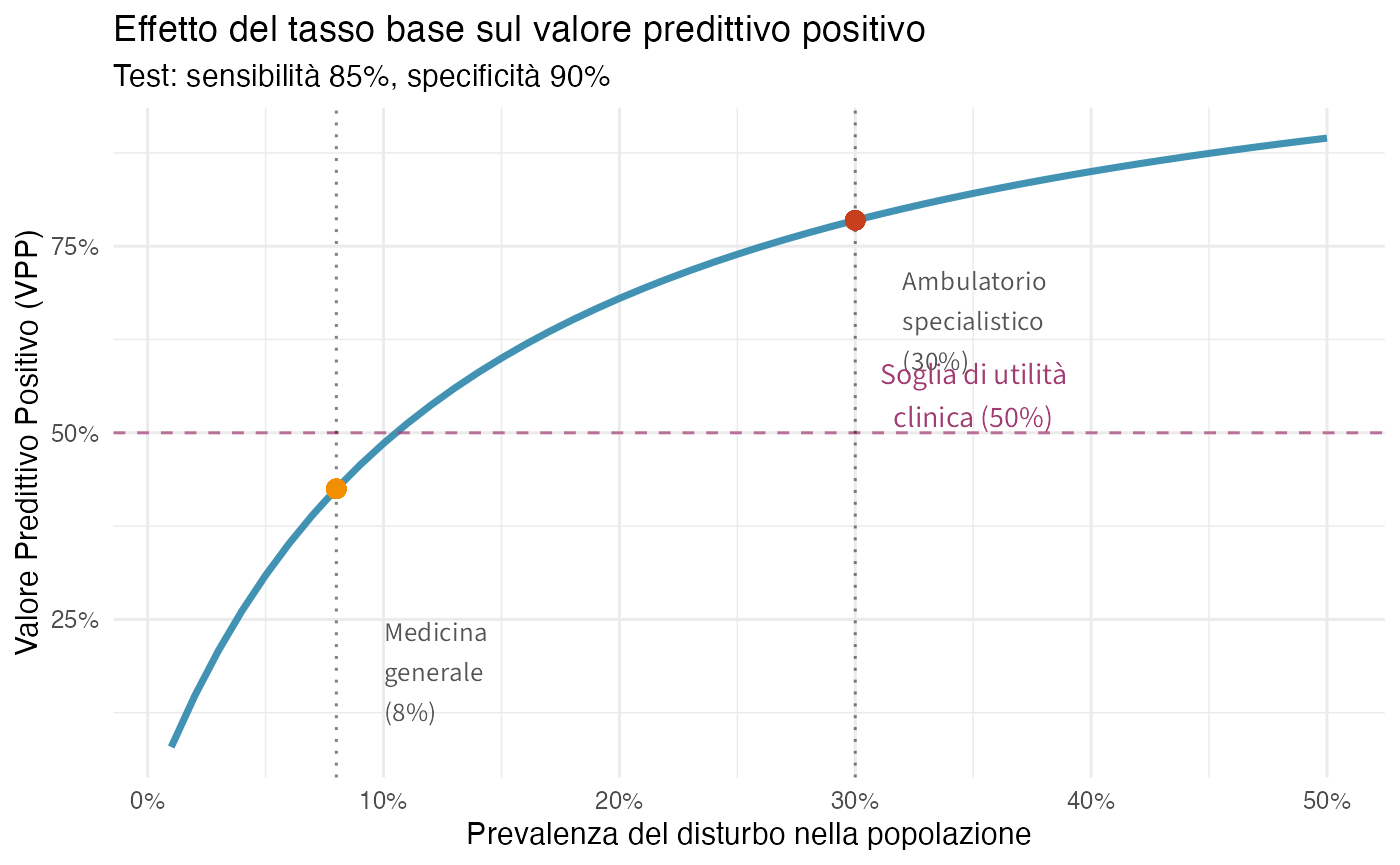
\includegraphics[width=0.85\linewidth,height=\textheight,keepaspectratio]{chapters/probability/05_bayes_theorem_files/figure-pdf/unnamed-chunk-15-1.png}

Il grafico illustra un fatto controintuitivo, ma fondamentale: l'utilità
clinica di un test dipende non solo dalle sue proprietà intrinseche
(sensibilità e specificità), ma anche dal contesto in cui viene
utilizzato. Lo stesso test che si rivela utile in un ambulatorio
specialistico (prevalenza 30\%, VPP circa 78\%) può risultare fuorviante
in medicina generale (prevalenza 8\%, VPP circa 43\%), generando più
falsi allarmi che diagnosi corrette.

Questa analisi evidenzia l'importanza cruciale di considerare il tasso
di base nella pratica clinica, mostrando che l'interpretazione di un
test positivo richiede sempre la contestualizzazione nella popolazione
di riferimento del paziente.

\end{tcolorbox}

\begin{tcolorbox}[enhanced jigsaw, arc=.35mm, breakable, colbacktitle=quarto-callout-note-color!10!white, opacityback=0, toprule=.15mm, rightrule=.15mm, colback=white, opacitybacktitle=0.6, leftrule=.75mm, coltitle=black, bottomtitle=1mm, left=2mm, toptitle=1mm, title=\textcolor{quarto-callout-note-color}{\faInfo}\hspace{0.5em}{Test diagnostico per il disturbo depressivo}, titlerule=0mm, bottomrule=.15mm, colframe=quarto-callout-note-color-frame]

Per spiegare come funziona il ragionamento bayesiano nella diagnosi
psicologica, prendiamo in considerazione uno scenario clinico
realistico.

\begin{Shaded}
\begin{Highlighting}[]
\CommentTok{\# Configurazione dello scenario: Screening per depressione maggiore in medicina generale}
\NormalTok{P\_D }\OtherTok{\textless{}{-}} \FloatTok{0.08}          \CommentTok{\# Prevalenza nella popolazione generale}
\NormalTok{sens }\OtherTok{\textless{}{-}} \FloatTok{0.85}         \CommentTok{\# Sensibilità del test di screening}
\NormalTok{spec }\OtherTok{\textless{}{-}} \FloatTok{0.90}         \CommentTok{\# Specificità del test}
\NormalTok{fp\_rate }\OtherTok{\textless{}{-}} \DecValTok{1} \SpecialCharTok{{-}}\NormalTok{ spec  }\CommentTok{\# Tasso di falsi positivi}

\FunctionTok{cat}\NormalTok{(}\StringTok{"Parametri dello scenario di screening:}\SpecialCharTok{\textbackslash{}n}\StringTok{"}\NormalTok{)}
\CommentTok{\#\textgreater{} Parametri dello scenario di screening:}
\FunctionTok{cat}\NormalTok{(}\StringTok{"Prevalenza depressione:"}\NormalTok{, P\_D}\SpecialCharTok{*}\DecValTok{100}\NormalTok{, }\StringTok{"\%}\SpecialCharTok{\textbackslash{}n}\StringTok{"}\NormalTok{)}
\CommentTok{\#\textgreater{} Prevalenza depressione: 8 \%}
\FunctionTok{cat}\NormalTok{(}\StringTok{"Sensibilità test:"}\NormalTok{, sens}\SpecialCharTok{*}\DecValTok{100}\NormalTok{, }\StringTok{"\%}\SpecialCharTok{\textbackslash{}n}\StringTok{"}\NormalTok{) }
\CommentTok{\#\textgreater{} Sensibilità test: 85 \%}
\FunctionTok{cat}\NormalTok{(}\StringTok{"Specificità test:"}\NormalTok{, spec}\SpecialCharTok{*}\DecValTok{100}\NormalTok{, }\StringTok{"\%}\SpecialCharTok{\textbackslash{}n}\StringTok{"}\NormalTok{)}
\CommentTok{\#\textgreater{} Specificità test: 90 \%}
\FunctionTok{cat}\NormalTok{(}\StringTok{"Tasso falsi positivi:"}\NormalTok{, fp\_rate}\SpecialCharTok{*}\DecValTok{100}\NormalTok{, }\StringTok{"\%}\SpecialCharTok{\textbackslash{}n\textbackslash{}n}\StringTok{"}\NormalTok{)}
\CommentTok{\#\textgreater{} Tasso falsi positivi: 10 \%}
\end{Highlighting}
\end{Shaded}

Applichiamo il teorema di Bayes per calcolare le probabilità rilevanti
per la decisione clinica:

\begin{Shaded}
\begin{Highlighting}[]
\CommentTok{\# Calcolo delle probabilità marginali dei risultati del test}
\NormalTok{P\_Tpos }\OtherTok{\textless{}{-}}\NormalTok{ sens }\SpecialCharTok{*}\NormalTok{ P\_D }\SpecialCharTok{+}\NormalTok{ fp\_rate }\SpecialCharTok{*}\NormalTok{ (}\DecValTok{1} \SpecialCharTok{{-}}\NormalTok{ P\_D)}
\NormalTok{P\_Tneg }\OtherTok{\textless{}{-}}\NormalTok{ (}\DecValTok{1} \SpecialCharTok{{-}}\NormalTok{ sens) }\SpecialCharTok{*}\NormalTok{ P\_D }\SpecialCharTok{+}\NormalTok{ spec }\SpecialCharTok{*}\NormalTok{ (}\DecValTok{1} \SpecialCharTok{{-}}\NormalTok{ P\_D)}

\FunctionTok{cat}\NormalTok{(}\StringTok{"Probabilità di test positivo:"}\NormalTok{, }\FunctionTok{round}\NormalTok{(P\_Tpos}\SpecialCharTok{*}\DecValTok{100}\NormalTok{, }\DecValTok{1}\NormalTok{), }\StringTok{"\%}\SpecialCharTok{\textbackslash{}n}\StringTok{"}\NormalTok{)}
\CommentTok{\#\textgreater{} Probabilità di test positivo: 16 \%}
\FunctionTok{cat}\NormalTok{(}\StringTok{"Probabilità di test negativo:"}\NormalTok{, }\FunctionTok{round}\NormalTok{(P\_Tneg}\SpecialCharTok{*}\DecValTok{100}\NormalTok{, }\DecValTok{1}\NormalTok{), }\StringTok{"\%}\SpecialCharTok{\textbackslash{}n\textbackslash{}n}\StringTok{"}\NormalTok{)}
\CommentTok{\#\textgreater{} Probabilità di test negativo: 84 \%}

\CommentTok{\# Calcolo delle probabilità a posteriori (valori predittivi)}
\NormalTok{P\_D\_given\_Tpos }\OtherTok{\textless{}{-}}\NormalTok{ (sens }\SpecialCharTok{*}\NormalTok{ P\_D) }\SpecialCharTok{/}\NormalTok{ P\_Tpos}
\NormalTok{P\_D\_given\_Tneg }\OtherTok{\textless{}{-}}\NormalTok{ ((}\DecValTok{1} \SpecialCharTok{{-}}\NormalTok{ sens) }\SpecialCharTok{*}\NormalTok{ P\_D) }\SpecialCharTok{/}\NormalTok{ P\_Tneg}

\FunctionTok{cat}\NormalTok{(}\StringTok{"Valore predittivo positivo (VPP):"}\NormalTok{, }\FunctionTok{round}\NormalTok{(P\_D\_given\_Tpos}\SpecialCharTok{*}\DecValTok{100}\NormalTok{, }\DecValTok{1}\NormalTok{), }\StringTok{"\%}\SpecialCharTok{\textbackslash{}n}\StringTok{"}\NormalTok{)}
\CommentTok{\#\textgreater{} Valore predittivo positivo (VPP): 42.5 \%}
\FunctionTok{cat}\NormalTok{(}\StringTok{"Valore predittivo negativo (VPN):"}\NormalTok{, }\FunctionTok{round}\NormalTok{((}\DecValTok{1} \SpecialCharTok{{-}}\NormalTok{ P\_D\_given\_Tneg)}\SpecialCharTok{*}\DecValTok{100}\NormalTok{, }\DecValTok{1}\NormalTok{), }\StringTok{"\%}\SpecialCharTok{\textbackslash{}n}\StringTok{"}\NormalTok{)}
\CommentTok{\#\textgreater{} Valore predittivo negativo (VPN): 98.6 \%}
\end{Highlighting}
\end{Shaded}

I risultati mostrano un pattern caratteristico dei contesti di screening
a bassa prevalenza:

\begin{Shaded}
\begin{Highlighting}[]
\CommentTok{\# Sintesi completa dell\textquotesingle{}analisi bayesiana}
\NormalTok{risultati }\OtherTok{\textless{}{-}} \FunctionTok{data.frame}\NormalTok{(}
  \AttributeTok{Misura =} \FunctionTok{c}\NormalTok{(}\StringTok{"Probabilità pre{-}test (prior)"}\NormalTok{, }
             \StringTok{"Sensibilità"}\NormalTok{, }
             \StringTok{"Specificità"}\NormalTok{,}
             \StringTok{"VPP (probabilità post{-}test positivo)"}\NormalTok{,}
             \StringTok{"Probabilità post{-}test negativo"}\NormalTok{),}
  \AttributeTok{Valore =} \FunctionTok{paste0}\NormalTok{(}\FunctionTok{round}\NormalTok{(}\FunctionTok{c}\NormalTok{(P\_D, sens, spec, P\_D\_given\_Tpos, P\_D\_given\_Tneg) }\SpecialCharTok{*} \DecValTok{100}\NormalTok{, }\DecValTok{1}\NormalTok{), }\StringTok{"\%"}\NormalTok{),}
  \AttributeTok{Interpretazione =} \FunctionTok{c}\NormalTok{(}\StringTok{"Prevalenza nella popolazione"}\NormalTok{,}
                     \StringTok{"P(T+ | Depressione)"}\NormalTok{,}
                     \StringTok{"P(T{-} | No Depressione)"}\NormalTok{, }
                     \StringTok{"P(Depressione | T+)"}\NormalTok{,}
                     \StringTok{"P(Depressione | T{-})"}\NormalTok{)}
\NormalTok{)}
\FunctionTok{print}\NormalTok{(risultati)}
\CommentTok{\#\textgreater{}                                 Misura Valore              Interpretazione}
\CommentTok{\#\textgreater{} 1         Probabilità pre{-}test (prior)     8\% Prevalenza nella popolazione}
\CommentTok{\#\textgreater{} 2                          Sensibilità    85\%          P(T+ | Depressione)}
\CommentTok{\#\textgreater{} 3                          Specificità    90\%       P(T{-} | No Depressione)}
\CommentTok{\#\textgreater{} 4 VPP (probabilità post{-}test positivo)  42.5\%          P(Depressione | T+)}
\CommentTok{\#\textgreater{} 5       Probabilità post{-}test negativo   1.4\%          P(Depressione | T{-})}
\end{Highlighting}
\end{Shaded}

L'analisi ha rivelato l'asimmetria informativa tipica dei test di
screening in popolazioni a bassa prevalenza. Un test positivo aumenta la
probabilità di depressione dall'8\% al 42\% circa, un aumento
considerevole, ma che lascia ancora una probabilità maggiore di assenza
di disturbo. Un test negativo, invece, riduce la probabilità a meno
dell'1.5\%, fornendo una rassicurazione quasi definitiva.

Questa asimmetria suggerisce che, in contesti di screening a bassa
prevalenza, il valore principale del test risiede nella sua capacità di
\textbf{escludere} la condizione (alto valore predittivo negativo)
piuttosto che di confermarla. Il clinico può quindi utilizzare il test
principalmente come strumento per identificare i casi che necessitano di
un'approfondita valutazione diagnostica, riconoscendo che un risultato
positivo richiede comunque una conferma ulteriore.

\end{tcolorbox}

\begin{tcolorbox}[enhanced jigsaw, arc=.35mm, breakable, colbacktitle=quarto-callout-note-color!10!white, opacityback=0, toprule=.15mm, rightrule=.15mm, colback=white, opacitybacktitle=0.6, leftrule=.75mm, coltitle=black, bottomtitle=1mm, left=2mm, toptitle=1mm, title=\textcolor{quarto-callout-note-color}{\faInfo}\hspace{0.5em}{Diagnostica sequenziale: l'accumulo di evidenze}, titlerule=0mm, bottomrule=.15mm, colframe=quarto-callout-note-color-frame]

Il ragionamento clinico raramente si basa su una sola fonte di
informazione. Il teorema di Bayes fornisce il quadro concettuale e
matematico ideale per integrare più fonti di informazione, trasformando
iterativamente la distribuzione a posteriori di un'osservazione nella
distribuzione a priori della successiva.

Consideriamo un caso clinico di valutazione dell'ADHD con due strumenti
complementari: un questionario somministrato ai genitori (sensibilità
0.80, specificità 0.85) e un'osservazione strutturata in classe
(sensibilità 0.75, specificità 0.88). Supponiamo che il disturbo abbia
una prevalenza del 5\% nella popolazione scolastica di riferimento.

\begin{Shaded}
\begin{Highlighting}[]
\CommentTok{\# Parametri iniziali della valutazione ADHD}
\NormalTok{P\_ADHD }\OtherTok{\textless{}{-}} \FloatTok{0.05}       \CommentTok{\# Prevalenza in popolazione scolare}
\NormalTok{sens\_T1 }\OtherTok{\textless{}{-}} \FloatTok{0.80}      \CommentTok{\# Questionario genitori}
\NormalTok{spec\_T1 }\OtherTok{\textless{}{-}} \FloatTok{0.85}
\NormalTok{sens\_T2 }\OtherTok{\textless{}{-}} \FloatTok{0.75}      \CommentTok{\# Osservazione in classe  }
\NormalTok{spec\_T2 }\OtherTok{\textless{}{-}} \FloatTok{0.88}
\end{Highlighting}
\end{Shaded}

\subsection*{Procedura di aggiornamento bayesiano
sequenziale}\label{procedura-di-aggiornamento-bayesiano-sequenziale}

\textbf{Fase 1: Probabilità iniziale e conversione in odds}

Partiamo dalla prevalenza di ADHD nella popolazione scolastica (5\%).
Convertiamo questa probabilità in odds per facilitare i calcoli
successivi.

\begin{Shaded}
\begin{Highlighting}[]
\CommentTok{\# Conversione della probabilità iniziale in odds}
\NormalTok{prior\_odds }\OtherTok{\textless{}{-}}\NormalTok{ P\_ADHD }\SpecialCharTok{/}\NormalTok{ (}\DecValTok{1} \SpecialCharTok{{-}}\NormalTok{ P\_ADHD)}
\FunctionTok{cat}\NormalTok{(}\StringTok{"Probabilità iniziale:"}\NormalTok{, P\_ADHD}\SpecialCharTok{*}\DecValTok{100}\NormalTok{, }\StringTok{"\%}\SpecialCharTok{\textbackslash{}n}\StringTok{"}\NormalTok{)}
\CommentTok{\#\textgreater{} Probabilità iniziale: 5 \%}
\FunctionTok{cat}\NormalTok{(}\StringTok{"Odds iniziali:"}\NormalTok{, }\FunctionTok{round}\NormalTok{(prior\_odds, }\DecValTok{4}\NormalTok{), }\StringTok{"}\SpecialCharTok{\textbackslash{}n\textbackslash{}n}\StringTok{"}\NormalTok{)}
\CommentTok{\#\textgreater{} Odds iniziali: 0.0526}
\end{Highlighting}
\end{Shaded}

\textbf{Fase 2: Calcolo dei rapporti di verosimiglianza}

Per ciascuno strumento diagnostico, calcoliamo il Likelihood Ratio
positivo (LR+), che quantifica quanto un test positivo aumenta la
probabilità di presenza del disturbo.

\begin{Shaded}
\begin{Highlighting}[]
\CommentTok{\# Calcolo dei likelihood ratios}
\NormalTok{LR\_pos\_T1 }\OtherTok{\textless{}{-}}\NormalTok{ sens\_T1 }\SpecialCharTok{/}\NormalTok{ (}\DecValTok{1} \SpecialCharTok{{-}}\NormalTok{ spec\_T1)}
\NormalTok{LR\_pos\_T2 }\OtherTok{\textless{}{-}}\NormalTok{ sens\_T2 }\SpecialCharTok{/}\NormalTok{ (}\DecValTok{1} \SpecialCharTok{{-}}\NormalTok{ spec\_T2)}

\FunctionTok{cat}\NormalTok{(}\StringTok{"Likelihood ratio questionario genitori:"}\NormalTok{, }\FunctionTok{round}\NormalTok{(LR\_pos\_T1, }\DecValTok{1}\NormalTok{), }\StringTok{"}\SpecialCharTok{\textbackslash{}n}\StringTok{"}\NormalTok{)}
\CommentTok{\#\textgreater{} Likelihood ratio questionario genitori: 5.3}
\FunctionTok{cat}\NormalTok{(}\StringTok{"Likelihood ratio osservazione in classe:"}\NormalTok{, }\FunctionTok{round}\NormalTok{(LR\_pos\_T2, }\DecValTok{1}\NormalTok{), }\StringTok{"}\SpecialCharTok{\textbackslash{}n\textbackslash{}n}\StringTok{"}\NormalTok{)}
\CommentTok{\#\textgreater{} Likelihood ratio osservazione in classe: 6.2}
\end{Highlighting}
\end{Shaded}

\textbf{Fase 3: Primo aggiornamento dopo questionario positivo}

Aggiorniamo gli odds moltiplicandoli per il LR+ del primo test e poi
riconvertiamo il risultato in probabilità per facilitare
l'interpretazione.

\begin{Shaded}
\begin{Highlighting}[]
\CommentTok{\# Primo aggiornamento bayesiano}
\NormalTok{post\_odds\_T1 }\OtherTok{\textless{}{-}}\NormalTok{ prior\_odds }\SpecialCharTok{*}\NormalTok{ LR\_pos\_T1}
\NormalTok{post\_prob\_T1 }\OtherTok{\textless{}{-}}\NormalTok{ post\_odds\_T1 }\SpecialCharTok{/}\NormalTok{ (}\DecValTok{1} \SpecialCharTok{+}\NormalTok{ post\_odds\_T1)}

\FunctionTok{cat}\NormalTok{(}\StringTok{"Odds dopo questionario positivo:"}\NormalTok{, }\FunctionTok{round}\NormalTok{(post\_odds\_T1, }\DecValTok{3}\NormalTok{), }\StringTok{"}\SpecialCharTok{\textbackslash{}n}\StringTok{"}\NormalTok{)}
\CommentTok{\#\textgreater{} Odds dopo questionario positivo: 0.281}
\FunctionTok{cat}\NormalTok{(}\StringTok{"Probabilità dopo questionario positivo:"}\NormalTok{, }\FunctionTok{round}\NormalTok{(post\_prob\_T1}\SpecialCharTok{*}\DecValTok{100}\NormalTok{, }\DecValTok{1}\NormalTok{), }\StringTok{"\%}\SpecialCharTok{\textbackslash{}n\textbackslash{}n}\StringTok{"}\NormalTok{)}
\CommentTok{\#\textgreater{} Probabilità dopo questionario positivo: 21.9 \%}
\end{Highlighting}
\end{Shaded}

\textbf{Fase 4: Secondo aggiornamento dopo osservazione positiva}

Il primo aggiornamento ci fornisce un nuovo prior, e a questo
applichiamo il LR+ del secondo test.

\begin{Shaded}
\begin{Highlighting}[]
\CommentTok{\# Secondo aggiornamento bayesiano}
\NormalTok{post\_odds\_both }\OtherTok{\textless{}{-}}\NormalTok{ post\_odds\_T1 }\SpecialCharTok{*}\NormalTok{ LR\_pos\_T2}
\NormalTok{post\_prob\_both }\OtherTok{\textless{}{-}}\NormalTok{ post\_odds\_both }\SpecialCharTok{/}\NormalTok{ (}\DecValTok{1} \SpecialCharTok{+}\NormalTok{ post\_odds\_both)}

\FunctionTok{cat}\NormalTok{(}\StringTok{"Odds dopo entrambi i test positivi:"}\NormalTok{, }\FunctionTok{round}\NormalTok{(post\_odds\_both, }\DecValTok{3}\NormalTok{), }\StringTok{"}\SpecialCharTok{\textbackslash{}n}\StringTok{"}\NormalTok{)}
\CommentTok{\#\textgreater{} Odds dopo entrambi i test positivi: 1.75}
\FunctionTok{cat}\NormalTok{(}\StringTok{"Probabilità dopo entrambi i test positivi:"}\NormalTok{, }\FunctionTok{round}\NormalTok{(post\_prob\_both}\SpecialCharTok{*}\DecValTok{100}\NormalTok{, }\DecValTok{1}\NormalTok{), }\StringTok{"\%}\SpecialCharTok{\textbackslash{}n}\StringTok{"}\NormalTok{)}
\CommentTok{\#\textgreater{} Probabilità dopo entrambi i test positivi: 63.7 \%}
\end{Highlighting}
\end{Shaded}

\textbf{Visualizzazione dell'aggiornamento sequenziale}

\begin{Shaded}
\begin{Highlighting}[]
\CommentTok{\# Preparazione dati per visualizzazione}
\NormalTok{df\_sequential }\OtherTok{\textless{}{-}} \FunctionTok{data.frame}\NormalTok{(}
  \AttributeTok{Momento =} \FunctionTok{factor}\NormalTok{(}\FunctionTok{c}\NormalTok{(}\StringTok{"Prior}\SpecialCharTok{\textbackslash{}n}\StringTok{(prevalenza)"}\NormalTok{, }\StringTok{"Dopo questionario}\SpecialCharTok{\textbackslash{}n}\StringTok{genitori (+)"}\NormalTok{, }
                     \StringTok{"Dopo osservazione}\SpecialCharTok{\textbackslash{}n}\StringTok{in classe (+)"}\NormalTok{),}
                   \AttributeTok{levels =} \FunctionTok{c}\NormalTok{(}\StringTok{"Prior}\SpecialCharTok{\textbackslash{}n}\StringTok{(prevalenza)"}\NormalTok{, }\StringTok{"Dopo questionario}\SpecialCharTok{\textbackslash{}n}\StringTok{genitori (+)"}\NormalTok{, }
                              \StringTok{"Dopo osservazione}\SpecialCharTok{\textbackslash{}n}\StringTok{in classe (+)"}\NormalTok{)),}
  \AttributeTok{Probabilita =} \FunctionTok{c}\NormalTok{(P\_ADHD, post\_prob\_T1, post\_prob\_both)}
\NormalTok{)}
\end{Highlighting}
\end{Shaded}

\begin{Shaded}
\begin{Highlighting}[]
\NormalTok{ymax }\OtherTok{\textless{}{-}} \FunctionTok{max}\NormalTok{(df\_sequential}\SpecialCharTok{$}\NormalTok{Probabilita) }\SpecialCharTok{*} \FloatTok{1.15}

\FunctionTok{ggplot}\NormalTok{(df\_sequential, }\FunctionTok{aes}\NormalTok{(}\AttributeTok{x =}\NormalTok{ Momento, }\AttributeTok{y =}\NormalTok{ Probabilita)) }\SpecialCharTok{+}
  \FunctionTok{geom\_col}\NormalTok{(}\AttributeTok{fill =} \StringTok{"\#4E79A7"}\NormalTok{, }\AttributeTok{alpha =} \FloatTok{0.8}\NormalTok{, }\AttributeTok{width =} \FloatTok{0.6}\NormalTok{) }\SpecialCharTok{+}
  \FunctionTok{geom\_text}\NormalTok{(}\FunctionTok{aes}\NormalTok{(}\AttributeTok{label =} \FunctionTok{sprintf}\NormalTok{(}\StringTok{"\%.1f\%\%"}\NormalTok{, Probabilita }\SpecialCharTok{*} \DecValTok{100}\NormalTok{)), }
            \AttributeTok{vjust =} \SpecialCharTok{{-}}\FloatTok{0.8}\NormalTok{, }\AttributeTok{size =} \FloatTok{4.5}\NormalTok{, }\AttributeTok{fontface =} \StringTok{"bold"}\NormalTok{) }\SpecialCharTok{+}
  \FunctionTok{geom\_line}\NormalTok{(}\FunctionTok{aes}\NormalTok{(}\AttributeTok{group =} \DecValTok{1}\NormalTok{), }\AttributeTok{linewidth =} \FloatTok{1.2}\NormalTok{, }\AttributeTok{color =} \StringTok{"\#2E5984"}\NormalTok{, }\AttributeTok{alpha =} \FloatTok{0.8}\NormalTok{) }\SpecialCharTok{+}
  \FunctionTok{geom\_point}\NormalTok{(}\AttributeTok{size =} \FloatTok{3.5}\NormalTok{, }\AttributeTok{color =} \StringTok{"\#2E5984"}\NormalTok{) }\SpecialCharTok{+}
  \FunctionTok{labs}\NormalTok{(}
    \AttributeTok{title =} \StringTok{"Aggiornamento bayesiano sequenziale nella diagnostica ADHD"}\NormalTok{,}
    \AttributeTok{subtitle =} \FunctionTok{paste0}\NormalTok{(}\StringTok{"LR+ questionario: "}\NormalTok{, }\FunctionTok{round}\NormalTok{(LR\_pos\_T1, }\DecValTok{1}\NormalTok{), }
                     \StringTok{" — LR+ osservazione: "}\NormalTok{, }\FunctionTok{round}\NormalTok{(LR\_pos\_T2, }\DecValTok{1}\NormalTok{)),}
    \AttributeTok{y =} \StringTok{"Probabilità di ADHD"}\NormalTok{,}
    \AttributeTok{x =} \ConstantTok{NULL}
\NormalTok{  ) }\SpecialCharTok{+}
  \FunctionTok{scale\_y\_continuous}\NormalTok{(}\AttributeTok{labels =}\NormalTok{ scales}\SpecialCharTok{::}\NormalTok{percent, }\AttributeTok{limits =} \FunctionTok{c}\NormalTok{(}\DecValTok{0}\NormalTok{, ymax)) }\SpecialCharTok{+}
  \FunctionTok{theme\_minimal}\NormalTok{() }\SpecialCharTok{+}
  \FunctionTok{theme}\NormalTok{(}\AttributeTok{plot.title =} \FunctionTok{element\_text}\NormalTok{(}\AttributeTok{face =} \StringTok{"bold"}\NormalTok{))}
\end{Highlighting}
\end{Shaded}

\begin{figure}[H]

\centering{

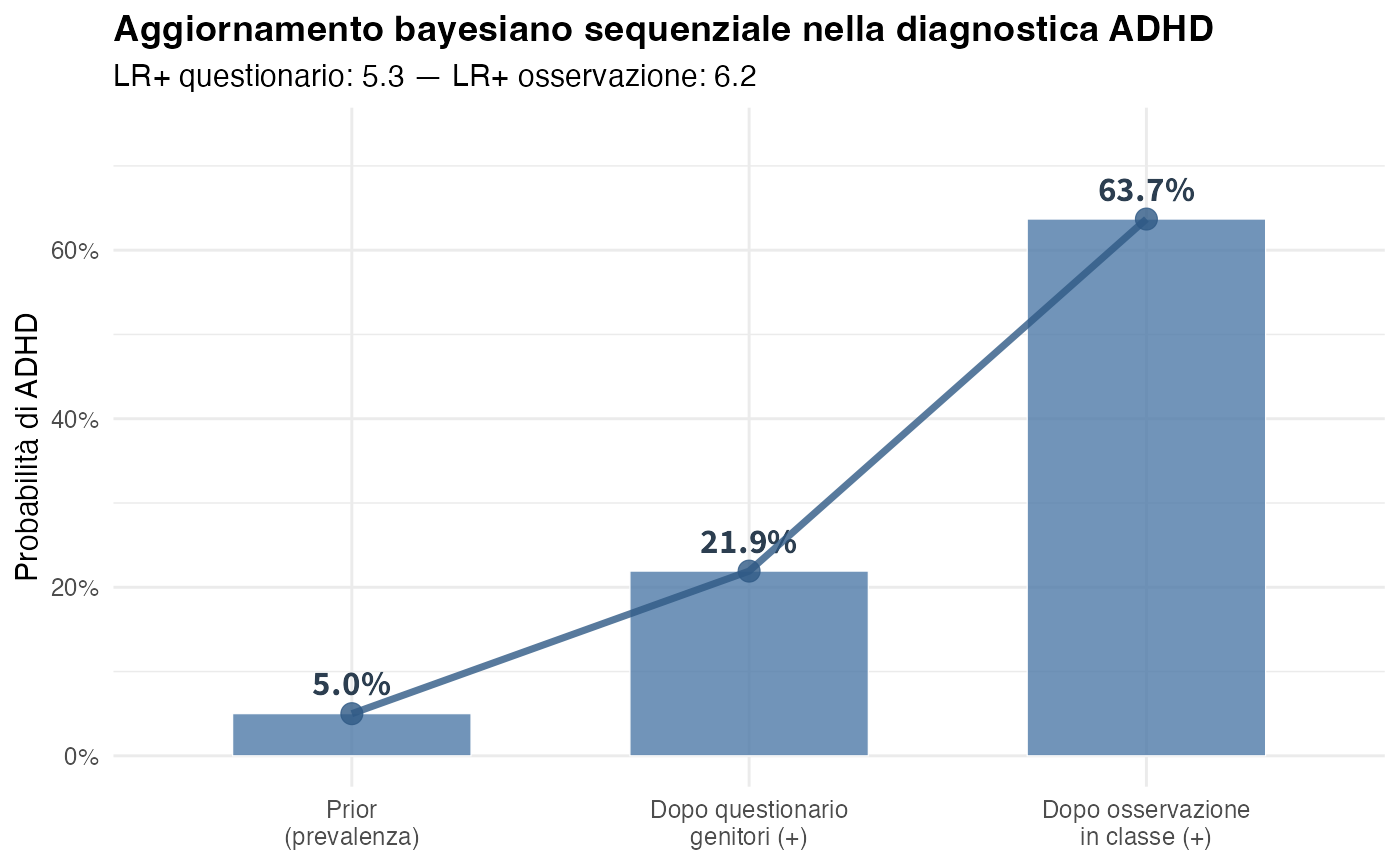
\includegraphics[width=0.85\linewidth,height=\textheight,keepaspectratio]{chapters/probability/05_bayes_theorem_files/figure-pdf/fig-sequential-1.png}

}

\caption{\label{fig-sequential}Aggiornamento bayesiano sequenziale nella
valutazione dell'ADHD. Ogni test positivo incrementa la probabilità in
modo cumulativo, con l'effetto che dipende dalla probabilità di partenza
e dalle caratteristiche dei test.}

\end{figure}%

\textbf{Interpretazione del processo cumulativo}

Il processo illustra come evidenze convergenti da fonti indipendenti
accumulino progressivamente il loro potere informativo. La probabilità
evolve dal \textbf{5\%} iniziale al \textbf{22\%} dopo il primo test e
al \textbf{64\%} dopo il secondo, raggiungendo una soglia clinicamente
significativa.

Ogni strumento diagnostico fornisce informazioni complementari: il
questionario per i genitori cattura la percezione del comportamento nel
contesto domestico, mentre l'osservazione in classe documenta le
manifestazioni nel contesto scolastico. L'assunzione di indipendenza
condizionale, ovvero che i due test forniscano informazioni indipendenti
dato lo stato reale del bambino, permette di moltiplicare i rapporti di
verosimiglianza, generando un effetto moltiplicativo sull'evidenza
complessiva.

Questo approccio sequenziale formalizza matematicamente la pratica
clinica reale, in cui le valutazioni si costruiscono progressivamente
attraverso l'integrazione sistematica di molteplici fonti di
informazione, trasformando un sospetto iniziale in una stima
probabilistica sempre più raffinata.

\end{tcolorbox}

\begin{tcolorbox}[enhanced jigsaw, arc=.35mm, breakable, colbacktitle=quarto-callout-note-color!10!white, opacityback=0, toprule=.15mm, rightrule=.15mm, colback=white, opacitybacktitle=0.6, leftrule=.75mm, coltitle=black, bottomtitle=1mm, left=2mm, toptitle=1mm, title=\textcolor{quarto-callout-note-color}{\faInfo}\hspace{0.5em}{Comorbilità e aggiornamento delle credenze diagnostiche}, titlerule=0mm, bottomrule=.15mm, colframe=quarto-callout-note-color-frame]

Il ragionamento clinico rappresenta un'applicazione particolarmente
illuminante del teorema di Bayes. Immaginiamo uno psicologo che si
accinge a valutare un nuovo paziente. Ancora prima di iniziare il
colloquio, lo psicologo possiede già una conoscenza di base derivante
dalla letteratura scientifica: sa che nella popolazione clinica di
riferimento la depressione ha una prevalenza di circa il 40\%. Questa
costituisce la sua probabilità a priori, il punto di partenza del suo
ragionamento diagnostico.

\begin{Shaded}
\begin{Highlighting}[]
\CommentTok{\# Definizione delle probabilità di base}
\NormalTok{P\_D }\OtherTok{\textless{}{-}} \FloatTok{0.40}          \CommentTok{\# Prevalenza depressione (prior)}
\NormalTok{P\_A\_given\_D }\OtherTok{\textless{}{-}} \FloatTok{0.60}  \CommentTok{\# Probabilità di ansia dato depressione}
\NormalTok{P\_A }\OtherTok{\textless{}{-}} \FloatTok{0.35}          \CommentTok{\# Prevalenza generale dell\textquotesingle{}ansia}
\end{Highlighting}
\end{Shaded}

La letteratura gli fornisce un'altra informazione cruciale: la
depressione e l'ansia presentano una rilevante comorbilità, con circa il
60\% dei pazienti depressi che manifesta anche sintomi ansiosi.
Contemporaneamente, egli ricorda che la prevalenza generale dell'ansia
nella stessa popolazione clinica è del 35\%.

Quando, durante il colloquio, emergono chiari segni di ansia, lo
psicologo si chiede: ``Come deve modificarsi la mia credenza riguardo
alla possibile depressione?'' Applicando il teorema di Bayes, scopre
che:

\begin{Shaded}
\begin{Highlighting}[]
\CommentTok{\# Applicazione del teorema di Bayes}
\NormalTok{P\_D\_given\_A }\OtherTok{\textless{}{-}}\NormalTok{ (P\_A\_given\_D }\SpecialCharTok{*}\NormalTok{ P\_D) }\SpecialCharTok{/}\NormalTok{ P\_A}

\CommentTok{\# Calcolo dello scenario complementare (ansia assente)}
\NormalTok{P\_not\_A }\OtherTok{\textless{}{-}} \DecValTok{1} \SpecialCharTok{{-}}\NormalTok{ P\_A}
\NormalTok{P\_D\_and\_A }\OtherTok{\textless{}{-}}\NormalTok{ P\_A\_given\_D }\SpecialCharTok{*}\NormalTok{ P\_D}
\NormalTok{P\_D\_and\_not\_A }\OtherTok{\textless{}{-}}\NormalTok{ P\_D }\SpecialCharTok{{-}}\NormalTok{ P\_D\_and\_A}
\NormalTok{P\_D\_given\_not\_A }\OtherTok{\textless{}{-}}\NormalTok{ P\_D\_and\_not\_A }\SpecialCharTok{/}\NormalTok{ P\_not\_A}

\FunctionTok{cat}\NormalTok{(}\StringTok{"Probabilità di depressione dato ansia:"}\NormalTok{, }\FunctionTok{round}\NormalTok{(P\_D\_given\_A }\SpecialCharTok{*} \DecValTok{100}\NormalTok{, }\DecValTok{1}\NormalTok{), }\StringTok{"\%}\SpecialCharTok{\textbackslash{}n}\StringTok{"}\NormalTok{)}
\CommentTok{\#\textgreater{} Probabilità di depressione dato ansia: 68.6 \%}
\end{Highlighting}
\end{Shaded}

La probabilità di depressione sale dal 40\% iniziale a circa il 69\%.
Questo quasi raddoppio della probabilità riflette il forte legame tra i
due disturbi.

Tuttavia, il ragionamento bayesiano consente di esplorare anche lo
scenario opposto:

\begin{Shaded}
\begin{Highlighting}[]
\FunctionTok{cat}\NormalTok{(}\StringTok{"Probabilità di depressione in assenza di ansia:"}\NormalTok{, }\FunctionTok{round}\NormalTok{(P\_D\_given\_not\_A }\SpecialCharTok{*} \DecValTok{100}\NormalTok{, }\DecValTok{1}\NormalTok{), }\StringTok{"\%}\SpecialCharTok{\textbackslash{}n}\StringTok{"}\NormalTok{)}
\CommentTok{\#\textgreater{} Probabilità di depressione in assenza di ansia: 24.6 \%}
\end{Highlighting}
\end{Shaded}

Cosa sarebbe successo se l'ansia fosse stata assente? In questo caso, la
probabilità di depressione sarebbe scesa drasticamente al 25\%, proprio
perché l'assenza di un sintomo così fortemente associato alla
depressione è un'informazione altrettanto significativa della sua
presenza.

\begin{Shaded}
\begin{Highlighting}[]
\CommentTok{\# Sintesi completa dell\textquotesingle{}aggiornamento diagnostico}
\NormalTok{risultati }\OtherTok{\textless{}{-}} \FunctionTok{data.frame}\NormalTok{(}
  \AttributeTok{Scenario =} \FunctionTok{c}\NormalTok{(}\StringTok{"Prima dell\textquotesingle{}osservazione"}\NormalTok{, }
               \StringTok{"Dopo osservare ansia"}\NormalTok{,}
               \StringTok{"Dopo escludere ansia"}\NormalTok{),}
  \AttributeTok{Probabilita =} \FunctionTok{c}\NormalTok{(P\_D, P\_D\_given\_A, P\_D\_given\_not\_A),}
  \AttributeTok{Percentuale =} \FunctionTok{paste0}\NormalTok{(}\FunctionTok{round}\NormalTok{(}\FunctionTok{c}\NormalTok{(P\_D, P\_D\_given\_A, P\_D\_given\_not\_A) }\SpecialCharTok{*} \DecValTok{100}\NormalTok{, }\DecValTok{1}\NormalTok{), }\StringTok{"\%"}\NormalTok{)}
\NormalTok{)}

\FunctionTok{print}\NormalTok{(risultati)}
\CommentTok{\#\textgreater{}                  Scenario Probabilita Percentuale}
\CommentTok{\#\textgreater{} 1 Prima dell\textquotesingle{}osservazione       0.400         40\%}
\CommentTok{\#\textgreater{} 2    Dopo osservare ansia       0.686       68.6\%}
\CommentTok{\#\textgreater{} 3    Dopo escludere ansia       0.246       24.6\%}
\end{Highlighting}
\end{Shaded}

Questo processo matematico formalizza e rende esplicito ciò che avviene
nella mente del clinico esperto: ogni nuovo dato e ogni sintomo
osservato modificano in modo quantificabile le probabilità delle varie
ipotesi diagnostiche. L'approccio bayesiano trasforma così il sospetto
clinico iniziale in una valutazione progressivamente più informata e
personalizzata, mostrando come l'accumulo di evidenze possa guidare il
ragionamento diagnostico in modo rigoroso e trasparente.

\end{tcolorbox}

\begin{tcolorbox}[enhanced jigsaw, arc=.35mm, breakable, colbacktitle=quarto-callout-note-color!10!white, opacityback=0, toprule=.15mm, rightrule=.15mm, colback=white, opacitybacktitle=0.6, leftrule=.75mm, coltitle=black, bottomtitle=1mm, left=2mm, toptitle=1mm, title=\textcolor{quarto-callout-note-color}{\faInfo}\hspace{0.5em}{Valore diagnostico incrementale di test multipli}, titlerule=0mm, bottomrule=.15mm, colframe=quarto-callout-note-color-frame]

Consideriamo ora la valutazione di un possibile caso di ADHD, per il
quale sono disponibili due strumenti complementari: un questionario per
i genitori e un'osservazione strutturata in classe.

\begin{Shaded}
\begin{Highlighting}[]
\CommentTok{\# Definizione dei parametri iniziali per la valutazione ADHD}
\NormalTok{P\_ADHD }\OtherTok{\textless{}{-}} \FloatTok{0.10}       \CommentTok{\# Prevalenza nella popolazione di riferimento}

\CommentTok{\# Caratteristiche del primo test: Questionario genitori (es. Conners)}
\NormalTok{sens\_T1 }\OtherTok{\textless{}{-}} \FloatTok{0.80}
\NormalTok{spec\_T1 }\OtherTok{\textless{}{-}} \FloatTok{0.85}
\NormalTok{fp\_T1 }\OtherTok{\textless{}{-}} \DecValTok{1} \SpecialCharTok{{-}}\NormalTok{ spec\_T1}

\CommentTok{\# Caratteristiche del secondo test: Osservazione strutturata in classe}
\NormalTok{sens\_T2 }\OtherTok{\textless{}{-}} \FloatTok{0.75}
\NormalTok{spec\_T2 }\OtherTok{\textless{}{-}} \FloatTok{0.90}
\NormalTok{fp\_T2 }\OtherTok{\textless{}{-}} \DecValTok{1} \SpecialCharTok{{-}}\NormalTok{ spec\_T2}
\end{Highlighting}
\end{Shaded}

Il clinico inizia la valutazione partendo dalla prevalenza generale
dell'ADHD nella popolazione di riferimento, che costituisce la
probabilità a priori del 10\%. Il primo strumento utilizzato è un
questionario per genitori che presenta una sensibilità dell'80\% e una
specificità dell'85\%.

\begin{Shaded}
\begin{Highlighting}[]
\CommentTok{\# Primo aggiornamento bayesiano: questionario positivo}
\NormalTok{P\_T1pos }\OtherTok{\textless{}{-}}\NormalTok{ sens\_T1 }\SpecialCharTok{*}\NormalTok{ P\_ADHD }\SpecialCharTok{+}\NormalTok{ fp\_T1 }\SpecialCharTok{*}\NormalTok{ (}\DecValTok{1} \SpecialCharTok{{-}}\NormalTok{ P\_ADHD)}
\NormalTok{P\_ADHD\_given\_T1pos }\OtherTok{\textless{}{-}}\NormalTok{ (sens\_T1 }\SpecialCharTok{*}\NormalTok{ P\_ADHD) }\SpecialCharTok{/}\NormalTok{ P\_T1pos}

\FunctionTok{cat}\NormalTok{(}\StringTok{"Probabilità dopo questionario positivo:"}\NormalTok{, }\FunctionTok{round}\NormalTok{(P\_ADHD\_given\_T1pos }\SpecialCharTok{*} \DecValTok{100}\NormalTok{, }\DecValTok{1}\NormalTok{), }\StringTok{"\%}\SpecialCharTok{\textbackslash{}n}\StringTok{"}\NormalTok{)}
\CommentTok{\#\textgreater{} Probabilità dopo questionario positivo: 37.2 \%}
\end{Highlighting}
\end{Shaded}

Quando il questionario risulta positivo, la probabilità di ADHD sale dal
10\% iniziale al 37\%. Questo primo aggiornamento rappresenta già un
incremento significativo, ma il clinico sa che una singola fonte di
informazione potrebbe non essere sufficiente per una diagnosi
affidabile.

Perciò, procede con il secondo strumento diagnostico: un'osservazione
strutturata in classe che offre una prospettiva complementare con una
sensibilità del 75\% e una specificità del 90\%.

\begin{Shaded}
\begin{Highlighting}[]
\CommentTok{\# Secondo aggiornamento: anche l\textquotesingle{}osservazione risulta positiva}
\CommentTok{\# Assumendo indipendenza condizionale dei test dato lo stato del paziente}
\NormalTok{P\_both\_pos\_given\_ADHD }\OtherTok{\textless{}{-}}\NormalTok{ sens\_T1 }\SpecialCharTok{*}\NormalTok{ sens\_T2}
\NormalTok{P\_both\_pos\_given\_no\_ADHD }\OtherTok{\textless{}{-}}\NormalTok{ fp\_T1 }\SpecialCharTok{*}\NormalTok{ fp\_T2}
\NormalTok{P\_ADHD\_T1\_T2 }\OtherTok{\textless{}{-}}\NormalTok{ P\_both\_pos\_given\_ADHD }\SpecialCharTok{*}\NormalTok{ P\_ADHD}
\NormalTok{P\_both\_pos }\OtherTok{\textless{}{-}}\NormalTok{ P\_ADHD\_T1\_T2 }\SpecialCharTok{+}\NormalTok{ P\_both\_pos\_given\_no\_ADHD }\SpecialCharTok{*}\NormalTok{ (}\DecValTok{1} \SpecialCharTok{{-}}\NormalTok{ P\_ADHD)}
\NormalTok{P\_ADHD\_given\_both\_pos }\OtherTok{\textless{}{-}}\NormalTok{ P\_ADHD\_T1\_T2 }\SpecialCharTok{/}\NormalTok{ P\_both\_pos}

\FunctionTok{cat}\NormalTok{(}\StringTok{"Probabilità dopo entrambi i test positivi:"}\NormalTok{, }\FunctionTok{round}\NormalTok{(P\_ADHD\_given\_both\_pos }\SpecialCharTok{*} \DecValTok{100}\NormalTok{, }\DecValTok{1}\NormalTok{), }\StringTok{"\%}\SpecialCharTok{\textbackslash{}n}\StringTok{"}\NormalTok{)}
\CommentTok{\#\textgreater{} Probabilità dopo entrambi i test positivi: 81.6 \%}
\end{Highlighting}
\end{Shaded}

Quando anche l'osservazione in classe risulta positiva, la probabilità
di ADHD raggiunge l'82\%. Questo secondo aggiornamento dimostra il
potere cumulativo dell'integrazione di evidenze multiple.

\begin{Shaded}
\begin{Highlighting}[]
\CommentTok{\# Sintesi completa dell\textquotesingle{}evoluzione diagnostica}
\NormalTok{evoluzione\_diagnostica }\OtherTok{\textless{}{-}} \FunctionTok{data.frame}\NormalTok{(}
  \AttributeTok{Fase =} \FunctionTok{c}\NormalTok{(}\StringTok{"Prior (prevalenza)"}\NormalTok{, }\StringTok{"Dopo questionario positivo"}\NormalTok{, }\StringTok{"Dopo entrambi i test positivi"}\NormalTok{),}
  \AttributeTok{Probabilita\_ADHD =} \FunctionTok{paste0}\NormalTok{(}\FunctionTok{round}\NormalTok{(}\FunctionTok{c}\NormalTok{(P\_ADHD, P\_ADHD\_given\_T1pos, P\_ADHD\_given\_both\_pos) }\SpecialCharTok{*} \DecValTok{100}\NormalTok{, }\DecValTok{1}\NormalTok{), }\StringTok{"\%"}\NormalTok{),}
  \AttributeTok{Incremento =} \FunctionTok{c}\NormalTok{(}\StringTok{"Baseline"}\NormalTok{, }\StringTok{"+27\%"}\NormalTok{, }\StringTok{"+45\% aggiuntivi"}\NormalTok{)}
\NormalTok{)}

\FunctionTok{print}\NormalTok{(evoluzione\_diagnostica)}
\CommentTok{\#\textgreater{}                            Fase Probabilita\_ADHD      Incremento}
\CommentTok{\#\textgreater{} 1            Prior (prevalenza)              10\%        Baseline}
\CommentTok{\#\textgreater{} 2    Dopo questionario positivo            37.2\%            +27\%}
\CommentTok{\#\textgreater{} 3 Dopo entrambi i test positivi            81.6\% +45\% aggiuntivi}
\end{Highlighting}
\end{Shaded}

Il risultato illustra il potere dell'integrazione di evidenze multiple.
Partendo da una prevalenza del 10\%, il primo test positivo porta la
probabilità al 37\%. Il secondo test positivo, proveniente da una fonte
indipendente (osservazione comportamentale vs.~report genitoriale),
fornisce un'informazione aggiuntiva che aumenta la probabilità all'82\%.
Questo cumulo moltiplicativo di evidenze trasforma una stima
epidemiologica generale in una valutazione clinicamente utile e
sufficientemente solida da poter guidare le decisioni terapeutiche.

\end{tcolorbox}

\begin{tcolorbox}[enhanced jigsaw, arc=.35mm, breakable, colbacktitle=quarto-callout-note-color!10!white, opacityback=0, toprule=.15mm, rightrule=.15mm, colback=white, opacitybacktitle=0.6, leftrule=.75mm, coltitle=black, bottomtitle=1mm, left=2mm, toptitle=1mm, title=\textcolor{quarto-callout-note-color}{\faInfo}\hspace{0.5em}{Confronto tra approccio bayesiano e frequentista}, titlerule=0mm, bottomrule=.15mm, colframe=quarto-callout-note-color-frame]

\subsubsection*{Esempio: Inferenza su moneta
sospetta}\label{esempio-inferenza-su-moneta-sospetta}

\textbf{Scenario}: 10 lanci di una moneta producono 8 risultati
``testa''. Dobbiamo valutare se la moneta sia equa (\(\theta = 0.5\)) o
sbilanciata verso testa (\(\theta = 0.7\)).

\begin{Shaded}
\begin{Highlighting}[]
\CommentTok{\# Configurazione dello scenario sperimentale}
\NormalTok{n\_lanci }\OtherTok{\textless{}{-}} \DecValTok{10}
\NormalTok{teste\_osservate }\OtherTok{\textless{}{-}} \DecValTok{8}

\CommentTok{\# Definizione delle ipotesi in competizione}
\NormalTok{theta\_equa }\OtherTok{\textless{}{-}} \FloatTok{0.5}
\NormalTok{theta\_sbilanciata }\OtherTok{\textless{}{-}} \FloatTok{0.7}

\CommentTok{\# Prior uniforme: inizialmente consideriamo equamente plausibili le due ipotesi}
\NormalTok{prior\_equa }\OtherTok{\textless{}{-}} \FloatTok{0.5}
\NormalTok{prior\_sbilanciata }\OtherTok{\textless{}{-}} \FloatTok{0.5}
\end{Highlighting}
\end{Shaded}

I dati osservati mostrano 8 teste su 10 lanci. Per valutare le due
ipotesi, calcoliamo prima quanto siano probabili questi dati sotto
ciascuna di esse:

\begin{Shaded}
\begin{Highlighting}[]
\CommentTok{\# Calcolo delle verosimiglianze per le due ipotesi}
\NormalTok{lik\_equa }\OtherTok{\textless{}{-}} \FunctionTok{dbinom}\NormalTok{(teste\_osservate, n\_lanci, theta\_equa)}
\NormalTok{lik\_sbilanciata }\OtherTok{\textless{}{-}} \FunctionTok{dbinom}\NormalTok{(teste\_osservate, n\_lanci, theta\_sbilanciata)}

\FunctionTok{cat}\NormalTok{(}\StringTok{"Verosimiglianza moneta equa:"}\NormalTok{, }\FunctionTok{round}\NormalTok{(lik\_equa, }\DecValTok{4}\NormalTok{), }\StringTok{"}\SpecialCharTok{\textbackslash{}n}\StringTok{"}\NormalTok{)}
\CommentTok{\#\textgreater{} Verosimiglianza moneta equa: 0.0439}
\FunctionTok{cat}\NormalTok{(}\StringTok{"Verosimiglianza moneta sbilanciata:"}\NormalTok{, }\FunctionTok{round}\NormalTok{(lik\_sbilanciata, }\DecValTok{4}\NormalTok{), }\StringTok{"}\SpecialCharTok{\textbackslash{}n}\StringTok{"}\NormalTok{)}
\CommentTok{\#\textgreater{} Verosimiglianza moneta sbilanciata: 0.234}
\FunctionTok{cat}\NormalTok{(}\StringTok{"Rapporto di verosimiglianza:"}\NormalTok{, }\FunctionTok{round}\NormalTok{(lik\_sbilanciata}\SpecialCharTok{/}\NormalTok{lik\_equa, }\DecValTok{1}\NormalTok{), }\StringTok{"}\SpecialCharTok{\textbackslash{}n}\StringTok{"}\NormalTok{)}
\CommentTok{\#\textgreater{} Rapporto di verosimiglianza: 5.3}
\end{Highlighting}
\end{Shaded}

I dati sono circa 5.3 volte più probabili se la moneta è sbilanciata
(\(\theta = 0.7\)) rispetto all'ipotesi di equità. Applichiamo ora il
teorema di Bayes per aggiornare le nostre credenze:

\begin{Shaded}
\begin{Highlighting}[]
\CommentTok{\# Aggiornamento bayesiano delle probabilità}
\NormalTok{evidenza\_totale }\OtherTok{\textless{}{-}}\NormalTok{ lik\_equa }\SpecialCharTok{*}\NormalTok{ prior\_equa }\SpecialCharTok{+}\NormalTok{ lik\_sbilanciata }\SpecialCharTok{*}\NormalTok{ prior\_sbilanciata}
\NormalTok{post\_equa }\OtherTok{\textless{}{-}}\NormalTok{ (lik\_equa }\SpecialCharTok{*}\NormalTok{ prior\_equa) }\SpecialCharTok{/}\NormalTok{ evidenza\_totale}
\NormalTok{post\_sbilanciata }\OtherTok{\textless{}{-}}\NormalTok{ (lik\_sbilanciata }\SpecialCharTok{*}\NormalTok{ prior\_sbilanciata) }\SpecialCharTok{/}\NormalTok{ evidenza\_totale}

\CommentTok{\# Sintesi dei risultati}
\NormalTok{risultati\_bayesiani }\OtherTok{\textless{}{-}} \FunctionTok{data.frame}\NormalTok{(}
  \AttributeTok{Metrica =} \FunctionTok{c}\NormalTok{(}\StringTok{"Verosimiglianza (moneta equa)"}\NormalTok{, }
              \StringTok{"Verosimiglianza (moneta sbilanciata)"}\NormalTok{, }
              \StringTok{"Probabilità a posteriori (equa)"}\NormalTok{, }
              \StringTok{"Probabilità a posteriori (sbilanciata)"}\NormalTok{),}
  \AttributeTok{Valore =} \FunctionTok{round}\NormalTok{(}\FunctionTok{c}\NormalTok{(lik\_equa, lik\_sbilanciata, post\_equa, post\_sbilanciata), }\DecValTok{4}\NormalTok{),}
  \AttributeTok{Interpretazione =} \FunctionTok{c}\NormalTok{(}\StringTok{"P(8 teste | θ = 0.5)"}\NormalTok{,}
                     \StringTok{"P(8 teste | θ = 0.7)"}\NormalTok{, }
                     \StringTok{"P(θ = 0.5 | 8 teste)"}\NormalTok{,}
                     \StringTok{"P(θ = 0.7 | 8 teste)"}\NormalTok{)}
\NormalTok{)}

\FunctionTok{print}\NormalTok{(risultati\_bayesiani)}
\CommentTok{\#\textgreater{}                                  Metrica Valore      Interpretazione}
\CommentTok{\#\textgreater{} 1          Verosimiglianza (moneta equa) 0.0439 P(8 teste | θ = 0.5)}
\CommentTok{\#\textgreater{} 2   Verosimiglianza (moneta sbilanciata) 0.2335 P(8 teste | θ = 0.7)}
\CommentTok{\#\textgreater{} 3        Probabilità a posteriori (equa) 0.1584 P(θ = 0.5 | 8 teste)}
\CommentTok{\#\textgreater{} 4 Probabilità a posteriori (sbilanciata) 0.8416 P(θ = 0.7 | 8 teste)}
\end{Highlighting}
\end{Shaded}

\textbf{Analisi frequentista}:

\begin{Shaded}
\begin{Highlighting}[]
\CommentTok{\# Calcolo del p{-}value frequentista}
\NormalTok{p\_value }\OtherTok{\textless{}{-}} \DecValTok{1} \SpecialCharTok{{-}} \FunctionTok{pbinom}\NormalTok{(}\DecValTok{8}\NormalTok{, }\DecValTok{10}\NormalTok{, }\FloatTok{0.5}\NormalTok{)  }\CommentTok{\# P(≥8 teste | θ = 0.5)}
\FunctionTok{cat}\NormalTok{(}\StringTok{"p{-}value frequentista:"}\NormalTok{, }\FunctionTok{round}\NormalTok{(p\_value, }\DecValTok{3}\NormalTok{), }\StringTok{"}\SpecialCharTok{\textbackslash{}n}\StringTok{"}\NormalTok{)}
\CommentTok{\#\textgreater{} p{-}value frequentista: 0.011}
\end{Highlighting}
\end{Shaded}

L'approccio frequentista calcolerebbe
\(P(\geq 8\ \text{teste} \mid \theta = 0.5) \approx 0.011\) e,
considerandolo statisticamente significativo (\(p < 0.05\)),
rifiuterebbe l'ipotesi di equità. Tuttavia, questo approccio non
quantifica quanto dovremmo credere che la moneta sia effettivamente
sbilanciata.

\textbf{Analisi bayesiana}: fornisce una risposta diretta alla domanda
di ricerca. I dati sono 5.3 volte più probabili sotto l'ipotesi di
sbilanciamento, portando la probabilità a posteriori della moneta
sbilanciata all'\textbf{84\%}. Questo rappresenta un supporto
sostanziale ma non conclusivo: permane un'incertezza non trascurabile
(16\% di probabilità residua per l'equità) che ulteriori osservazioni
potrebbero ridurre.

\textbf{Contrasto metodologico}: mentre il test frequentista valuta
quanto sia inusuale osservare dati così estremi assumendo vera l'ipotesi
nulla, l'approccio bayesiano quantifica direttamente la plausibilità
relativa delle diverse ipotesi alla luce dei dati osservati. Il
risultato bayesiano (84\% di probabilità per lo sbilanciamento) fornisce
una misura più intuitiva e direttamente interpretabile dell'evidenza
rispetto al valore-\(p\) frequentista.

\end{tcolorbox}

\section{Aggiornamento bayesiano con distribuzioni
continue}\label{aggiornamento-bayesiano-con-distribuzioni-continue}

Quando il parametro di interesse è continuo, come la probabilità
sottostante di un certo comportamento, il teorema di Bayes opera su
\textbf{distribuzioni di probabilità} piuttosto che su probabilità
discrete.

\subsection{Il modello Beta-Binomiale}\label{il-modello-beta-binomiale}

La distribuzione Beta è la scelta naturale per rappresentare le credenze
riguardanti le probabilità \(\theta \in [0,1]\). In combinazione con i
dati binomiali, il processo di aggiornamento assume una forma
particolarmente elegante (per una trattazione approfondita, si vedano i
Capitoli 12 e 13 del manuale didattico e i materiali complementari
disponibili sul \emph{companion site}).

\begin{tcolorbox}[enhanced jigsaw, arc=.35mm, breakable, colbacktitle=quarto-callout-note-color!10!white, opacityback=0, toprule=.15mm, rightrule=.15mm, colback=white, opacitybacktitle=0.6, leftrule=.75mm, coltitle=black, bottomtitle=1mm, left=2mm, toptitle=1mm, title=\textcolor{quarto-callout-note-color}{\faInfo}\hspace{0.5em}{Proprietà di coniugazione Beta-Binomiale}, titlerule=0mm, bottomrule=.15mm, colframe=quarto-callout-note-color-frame]

\textbf{Distribuzione a priori}:
\(\theta \sim \text{Beta}(\alpha, \beta)\).

\textbf{Modello dei dati}: \(k\) successi in \(n\) prove indipendenti.

\textbf{Distribuzione a posteriori}:
\(\theta \mid \text{dati} \sim \text{Beta}(\alpha + k, \beta + n - k)\).

\textbf{Interpretazione}: I parametri \(\alpha\) e \(\beta\) possono
essere interpretati come ``pseudo-osservazioni'' precedenti,
rispettivamente successi e fallimenti, che vengono aggiornati sommando
le evidenze empiriche osservate.

\end{tcolorbox}

Questa proprietà di coniugazione rende l'aggiornamento bayesiano
computazionalmente semplice e concettualmente trasparente, poiché le
distribuzioni a priori e a posteriori appartengono alla stessa famiglia
parametrica.

\begin{Shaded}
\begin{Highlighting}[]
\CommentTok{\# Scenario: Test a scelta multipla con 4 opzioni}
\CommentTok{\# Prior centrato sull\textquotesingle{}ipotesi di risposta casuale (1/4 = 0.25)}
\NormalTok{alpha\_prior }\OtherTok{\textless{}{-}} \DecValTok{1}
\NormalTok{beta\_prior }\OtherTok{\textless{}{-}} \DecValTok{3}  \CommentTok{\# Media prior = 1/(1+3) = 0.25}

\CommentTok{\# Dati osservati: 12 risposte corrette su 30}
\NormalTok{n\_obs }\OtherTok{\textless{}{-}} \DecValTok{30}
\NormalTok{k\_success }\OtherTok{\textless{}{-}} \DecValTok{12}

\CommentTok{\# Aggiornamento bayesiano}
\NormalTok{alpha\_post }\OtherTok{\textless{}{-}}\NormalTok{ alpha\_prior }\SpecialCharTok{+}\NormalTok{ k\_success}
\NormalTok{beta\_post }\OtherTok{\textless{}{-}}\NormalTok{ beta\_prior }\SpecialCharTok{+}\NormalTok{ (n\_obs }\SpecialCharTok{{-}}\NormalTok{ k\_success)}

\CommentTok{\# Griglia per visualizzazione}
\NormalTok{theta\_seq }\OtherTok{\textless{}{-}} \FunctionTok{seq}\NormalTok{(}\DecValTok{0}\NormalTok{, }\DecValTok{1}\NormalTok{, }\AttributeTok{length.out =} \DecValTok{500}\NormalTok{)}

\CommentTok{\# Calcolo delle densità}
\NormalTok{prior\_dens }\OtherTok{\textless{}{-}} \FunctionTok{dbeta}\NormalTok{(theta\_seq, alpha\_prior, beta\_prior)}
\NormalTok{posterior\_dens }\OtherTok{\textless{}{-}} \FunctionTok{dbeta}\NormalTok{(theta\_seq, alpha\_post, beta\_post)}

\CommentTok{\# Normalizzazione della verosimiglianza per visualizzazione}
\NormalTok{likelihood\_dens }\OtherTok{\textless{}{-}} \FunctionTok{dbinom}\NormalTok{(k\_success, }\AttributeTok{size =}\NormalTok{ n\_obs, }\AttributeTok{prob =}\NormalTok{ theta\_seq)}
\NormalTok{likelihood\_dens }\OtherTok{\textless{}{-}}\NormalTok{ likelihood\_dens }\SpecialCharTok{/} \FunctionTok{max}\NormalTok{(likelihood\_dens) }\SpecialCharTok{*} \FunctionTok{max}\NormalTok{(posterior\_dens)}

\CommentTok{\# Preparazione dati per visualizzazione}
\NormalTok{df\_beta }\OtherTok{\textless{}{-}} \FunctionTok{data.frame}\NormalTok{(}
  \AttributeTok{theta =}\NormalTok{ theta\_seq,}
  \AttributeTok{Prior =}\NormalTok{ prior\_dens,}
  \AttributeTok{Verosimiglianza =}\NormalTok{ likelihood\_dens,}
  \AttributeTok{Posterior =}\NormalTok{ posterior\_dens}
\NormalTok{)}

\NormalTok{df\_beta\_long }\OtherTok{\textless{}{-}}\NormalTok{ df\_beta }\SpecialCharTok{\%\textgreater{}\%}
  \FunctionTok{pivot\_longer}\NormalTok{(}\AttributeTok{cols =} \FunctionTok{c}\NormalTok{(Prior, Verosimiglianza, Posterior),}
               \AttributeTok{names\_to =} \StringTok{"Componente"}\NormalTok{, }\AttributeTok{values\_to =} \StringTok{"Densita"}\NormalTok{)}

\FunctionTok{ggplot}\NormalTok{(df\_beta\_long, }\FunctionTok{aes}\NormalTok{(}\AttributeTok{x =}\NormalTok{ theta, }\AttributeTok{y =}\NormalTok{ Densita, }\AttributeTok{color =}\NormalTok{ Componente, }\AttributeTok{linetype =}\NormalTok{ Componente)) }\SpecialCharTok{+}
  \FunctionTok{geom\_line}\NormalTok{(}\AttributeTok{linewidth =} \FloatTok{1.2}\NormalTok{) }\SpecialCharTok{+}
  \FunctionTok{geom\_vline}\NormalTok{(}\AttributeTok{xintercept =} \FloatTok{0.25}\NormalTok{, }\AttributeTok{linetype =} \StringTok{"dotted"}\NormalTok{, }\AttributeTok{alpha =} \FloatTok{0.5}\NormalTok{) }\SpecialCharTok{+}
  \FunctionTok{annotate}\NormalTok{(}\StringTok{"text"}\NormalTok{, }\AttributeTok{x =} \FloatTok{0.27}\NormalTok{, }\AttributeTok{y =} \FunctionTok{max}\NormalTok{(posterior\_dens) }\SpecialCharTok{*} \FloatTok{0.9}\NormalTok{, }
           \AttributeTok{label =} \StringTok{"Risposta}\SpecialCharTok{\textbackslash{}n}\StringTok{casuale"}\NormalTok{, }\AttributeTok{hjust =} \DecValTok{0}\NormalTok{, }\AttributeTok{size =} \FloatTok{3.5}\NormalTok{) }\SpecialCharTok{+}
  \FunctionTok{scale\_color\_manual}\NormalTok{(}\AttributeTok{values =} \FunctionTok{c}\NormalTok{(}\StringTok{"Prior"} \OtherTok{=} \StringTok{"\#E63946"}\NormalTok{, }\StringTok{"Verosimiglianza"} \OtherTok{=} \StringTok{"\#457B9D"}\NormalTok{, }\StringTok{"Posterior"} \OtherTok{=} \StringTok{"\#2A9D8F"}\NormalTok{)) }\SpecialCharTok{+}
  \FunctionTok{scale\_linetype\_manual}\NormalTok{(}\AttributeTok{values =} \FunctionTok{c}\NormalTok{(}\StringTok{"Prior"} \OtherTok{=} \StringTok{"dashed"}\NormalTok{, }\StringTok{"Verosimiglianza"} \OtherTok{=} \StringTok{"dotted"}\NormalTok{, }\StringTok{"Posterior"} \OtherTok{=} \StringTok{"solid"}\NormalTok{)) }\SpecialCharTok{+}
  \FunctionTok{labs}\NormalTok{(}
    \AttributeTok{title =} \StringTok{"Aggiornamento bayesiano nel modello Beta{-}Binomiale"}\NormalTok{,}
    \AttributeTok{subtitle =} \StringTok{"12 risposte corrette su 30 in un test a 4 opzioni"}\NormalTok{,}
    \AttributeTok{x =} \FunctionTok{expression}\NormalTok{(theta }\SpecialCharTok{\textasciitilde{}} \StringTok{"(probabilità di risposta corretta)"}\NormalTok{),}
    \AttributeTok{y =} \StringTok{"Densità di probabilità"}
\NormalTok{  ) }\SpecialCharTok{+}
  \FunctionTok{theme\_minimal}\NormalTok{() }
\end{Highlighting}
\end{Shaded}

\begin{figure}[H]

\centering{

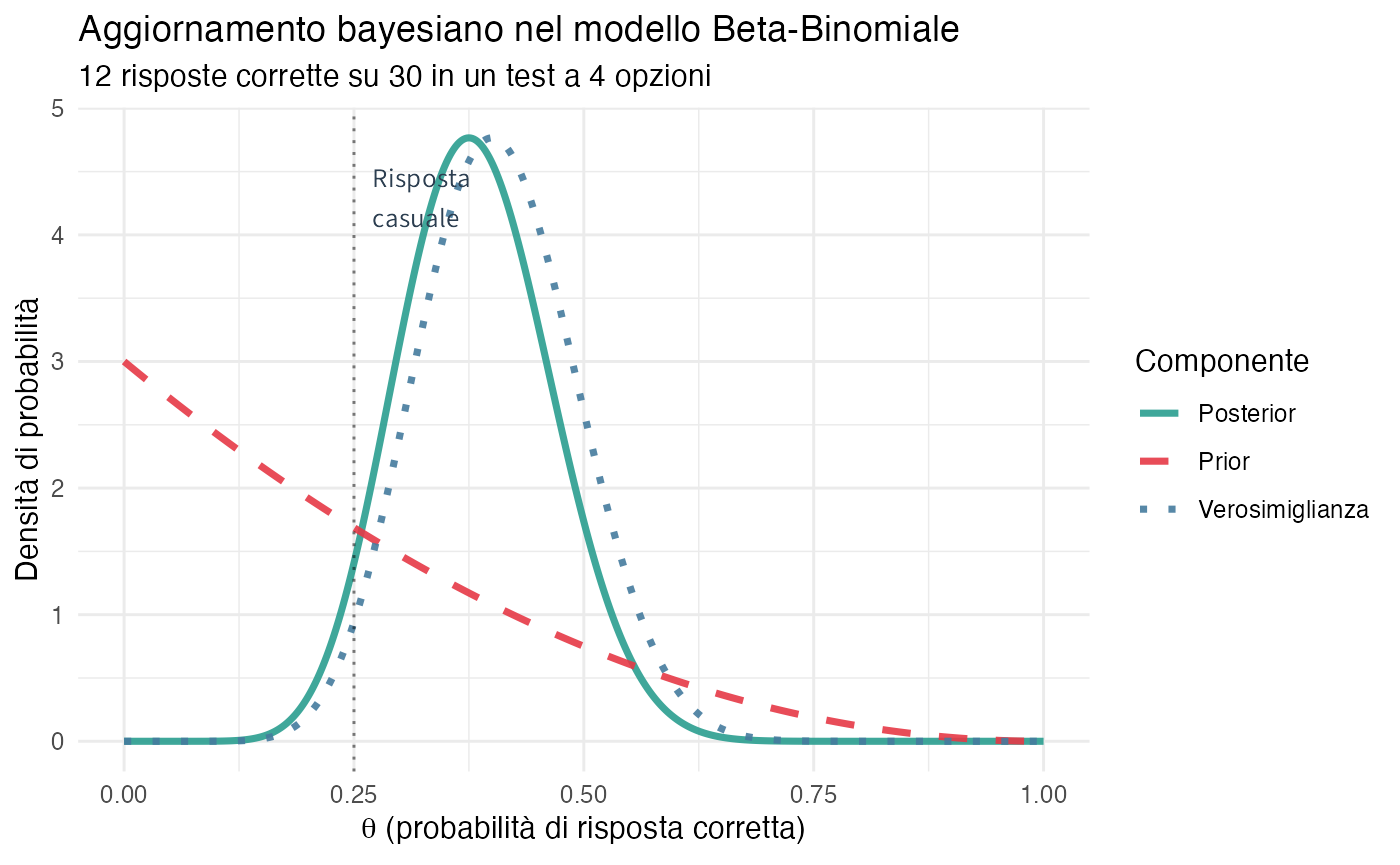
\includegraphics[width=0.85\linewidth,height=\textheight,keepaspectratio]{chapters/probability/05_bayes_theorem_files/figure-pdf/fig-beta-binomial-1.png}

}

\caption{\label{fig-beta-binomial}Aggiornamento bayesiano nel modello
Beta-Binomiale. La distribuzione a posteriori rappresenta una sintesi
tra le credenze iniziali (prior) e l'informazione contenuta nei dati
(likelihood).}

\end{figure}%

La visualizzazione illustra il meccanismo dell'aggiornamento bayesiano.
La distribuzione a priori (tratteggiata in rosso) è centrata su 0.25 e
rappresenta la credenza iniziale che lo studente stia rispondendo a
caso. La funzione di verosimiglianza (punteggiata in blu) indica che i
dati osservati (12/30, ovvero il 40\% di risposte corrette) sono
massimamente compatibili con un valore di \(\theta\) intorno a 0.40. La
distribuzione a posteriori (verde solida) rappresenta la sintesi
bayesiana: è spostata verso il dato osservato, ma non completamente,
riflettendo l'influenza residua del prior.

\begin{Shaded}
\begin{Highlighting}[]
\CommentTok{\# Confronto tra diversi approcci inferenziali}
\NormalTok{prior\_mean }\OtherTok{\textless{}{-}}\NormalTok{ alpha\_prior }\SpecialCharTok{/}\NormalTok{ (alpha\_prior }\SpecialCharTok{+}\NormalTok{ beta\_prior)}
\NormalTok{post\_mean }\OtherTok{\textless{}{-}}\NormalTok{ alpha\_post }\SpecialCharTok{/}\NormalTok{ (alpha\_post }\SpecialCharTok{+}\NormalTok{ beta\_post)}
\NormalTok{mle }\OtherTok{\textless{}{-}}\NormalTok{ k\_success }\SpecialCharTok{/}\NormalTok{ n\_obs}

\FunctionTok{data.frame}\NormalTok{(}
  \AttributeTok{Metodo =} \FunctionTok{c}\NormalTok{(}\StringTok{"Media a priori"}\NormalTok{, }\StringTok{"Stima di massima verosimiglianza"}\NormalTok{, }\StringTok{"Media a posteriori"}\NormalTok{),}
  \AttributeTok{Valore =} \FunctionTok{round}\NormalTok{(}\FunctionTok{c}\NormalTok{(prior\_mean, mle, post\_mean), }\DecValTok{3}\NormalTok{),}
  \AttributeTok{Interpretazione =} \FunctionTok{c}\NormalTok{(}\StringTok{"Credenza iniziale"}\NormalTok{, }
                      \StringTok{"Solo informazione dai dati"}\NormalTok{, }
                      \StringTok{"Sintesi tra prior e dati"}\NormalTok{)}
\NormalTok{)}
\CommentTok{\#\textgreater{}                             Metodo Valore            Interpretazione}
\CommentTok{\#\textgreater{} 1                   Media a priori  0.250          Credenza iniziale}
\CommentTok{\#\textgreater{} 2 Stima di massima verosimiglianza  0.400 Solo informazione dai dati}
\CommentTok{\#\textgreater{} 3               Media a posteriori  0.382   Sintesi tra prior e dati}
\end{Highlighting}
\end{Shaded}

Il confronto numerico mostra come l'approccio bayesiano fornisca una
stima intermedia tra la credenza iniziale e l'evidenza empirica,
ponderando entrambe le fonti di informazione in modo coerente.

\subsection{Intervalli di credibilità
bayesiani}\label{intervalli-di-credibilituxe0-bayesiani}

Mentre gli intervalli di confidenza frequentisti descrivono le proprietà
di una procedura di stima, gli intervalli di credibilità bayesiani
forniscono una quantificazione diretta dell'incertezza relativa al
parametro di interesse.

\begin{Shaded}
\begin{Highlighting}[]
\CommentTok{\# Calcolo dell\textquotesingle{}intervallo di credibilità}
\NormalTok{ci\_lower }\OtherTok{\textless{}{-}} \FunctionTok{qbeta}\NormalTok{(}\FloatTok{0.025}\NormalTok{, alpha\_post, beta\_post)}
\NormalTok{ci\_upper }\OtherTok{\textless{}{-}} \FunctionTok{qbeta}\NormalTok{(}\FloatTok{0.975}\NormalTok{, alpha\_post, beta\_post)}

\CommentTok{\# Creazione del dataframe per la visualizzazione}
\NormalTok{df\_posterior }\OtherTok{\textless{}{-}} \FunctionTok{data.frame}\NormalTok{(}
  \AttributeTok{theta =}\NormalTok{ theta\_seq,}
  \AttributeTok{densita =}\NormalTok{ posterior\_dens}
\NormalTok{)}

\FunctionTok{ggplot}\NormalTok{(df\_posterior, }\FunctionTok{aes}\NormalTok{(}\AttributeTok{x =}\NormalTok{ theta, }\AttributeTok{y =}\NormalTok{ densita)) }\SpecialCharTok{+}
  \FunctionTok{geom\_line}\NormalTok{(}\AttributeTok{linewidth =} \FloatTok{1.2}\NormalTok{, }\AttributeTok{color =} \StringTok{"\#2A9D8F"}\NormalTok{) }\SpecialCharTok{+}
  \FunctionTok{geom\_area}\NormalTok{(}\AttributeTok{data =}\NormalTok{ df\_posterior }\SpecialCharTok{\%\textgreater{}\%} \FunctionTok{filter}\NormalTok{(theta }\SpecialCharTok{\textgreater{}=}\NormalTok{ ci\_lower }\SpecialCharTok{\&}\NormalTok{ theta }\SpecialCharTok{\textless{}=}\NormalTok{ ci\_upper),}
            \FunctionTok{aes}\NormalTok{(}\AttributeTok{x =}\NormalTok{ theta, }\AttributeTok{y =}\NormalTok{ densita), }\AttributeTok{fill =} \StringTok{"\#2A9D8F"}\NormalTok{, }\AttributeTok{alpha =} \FloatTok{0.3}\NormalTok{) }\SpecialCharTok{+}
  \FunctionTok{geom\_vline}\NormalTok{(}\AttributeTok{xintercept =} \FunctionTok{c}\NormalTok{(ci\_lower, ci\_upper), }\AttributeTok{linetype =} \StringTok{"dashed"}\NormalTok{, }\AttributeTok{color =} \StringTok{"\#2A9D8F"}\NormalTok{) }\SpecialCharTok{+}
  \FunctionTok{geom\_vline}\NormalTok{(}\AttributeTok{xintercept =}\NormalTok{ post\_mean, }\AttributeTok{color =} \StringTok{"\#E63946"}\NormalTok{, }\AttributeTok{linewidth =} \DecValTok{1}\NormalTok{) }\SpecialCharTok{+}
  \FunctionTok{annotate}\NormalTok{(}\StringTok{"text"}\NormalTok{, }\AttributeTok{x =}\NormalTok{ post\_mean }\SpecialCharTok{+} \FloatTok{0.02}\NormalTok{, }\AttributeTok{y =} \FunctionTok{max}\NormalTok{(posterior\_dens) }\SpecialCharTok{*} \FloatTok{0.7}\NormalTok{,}
           \AttributeTok{label =} \FunctionTok{paste0}\NormalTok{(}\StringTok{"Media: "}\NormalTok{, }\FunctionTok{round}\NormalTok{(post\_mean, }\DecValTok{3}\NormalTok{)), }
           \AttributeTok{hjust =} \DecValTok{0}\NormalTok{, }\AttributeTok{color =} \StringTok{"\#E63946"}\NormalTok{, }\AttributeTok{size =} \DecValTok{4}\NormalTok{) }\SpecialCharTok{+}
  \FunctionTok{annotate}\NormalTok{(}\StringTok{"text"}\NormalTok{, }\AttributeTok{x =} \FunctionTok{mean}\NormalTok{(}\FunctionTok{c}\NormalTok{(ci\_lower, ci\_upper)), }\AttributeTok{y =} \FunctionTok{max}\NormalTok{(posterior\_dens) }\SpecialCharTok{*} \FloatTok{0.4}\NormalTok{,}
           \AttributeTok{label =} \FunctionTok{paste0}\NormalTok{(}\StringTok{"IC 95\%}\SpecialCharTok{\textbackslash{}n}\StringTok{["}\NormalTok{, }\FunctionTok{round}\NormalTok{(ci\_lower, }\DecValTok{3}\NormalTok{), }\StringTok{", "}\NormalTok{, }\FunctionTok{round}\NormalTok{(ci\_upper, }\DecValTok{3}\NormalTok{), }\StringTok{"]"}\NormalTok{),}
           \AttributeTok{color =} \StringTok{"\#1D3557"}\NormalTok{, }\AttributeTok{size =} \DecValTok{4}\NormalTok{) }\SpecialCharTok{+}
  \FunctionTok{labs}\NormalTok{(}
    \AttributeTok{title =} \StringTok{"Distribuzione a posteriori con intervallo di credibilità"}\NormalTok{,}
    \AttributeTok{subtitle =} \StringTok{"Quantificazione completa dell\textquotesingle{}incertezza sul parametro θ"}\NormalTok{,}
    \AttributeTok{x =} \FunctionTok{expression}\NormalTok{(theta }\SpecialCharTok{\textasciitilde{}} \StringTok{"(probabilità di risposta corretta)"}\NormalTok{),}
    \AttributeTok{y =} \StringTok{"Densità a posteriori"}
\NormalTok{  ) }\SpecialCharTok{+}
  \FunctionTok{theme\_minimal}\NormalTok{()}
\end{Highlighting}
\end{Shaded}

\begin{figure}[H]

\centering{

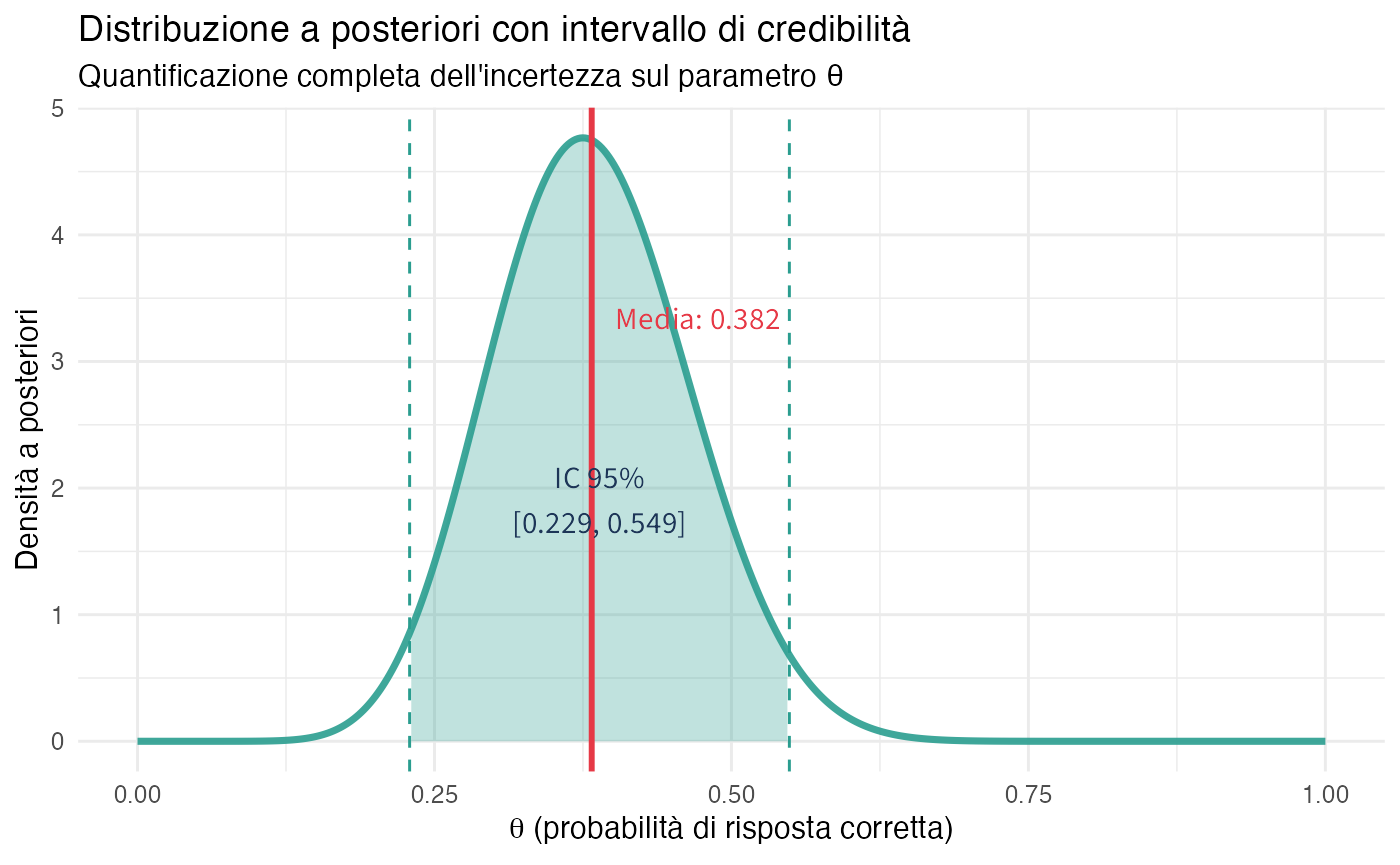
\includegraphics[width=0.85\linewidth,height=\textheight,keepaspectratio]{chapters/probability/05_bayes_theorem_files/figure-pdf/fig-credibility-1.png}

}

\caption{\label{fig-credibility}Distribuzione a posteriori con
intervallo di credibilità al 95\%. L'area ombreggiata rappresenta la
regione in cui assegniamo probabilità 0.95 che si trovi il vero valore
del parametro.}

\end{figure}%

\textbf{Interpretazione epistemica diretta}: l'intervallo {[}0.23,
0.55{]} rappresenta la regione in cui, alla luce dei dati osservati e
delle nostre credenze iniziali, assegniamo una probabilità del 95\% che
si trovi il vero valore del parametro θ.

Questa interpretazione differisce fondamentalmente da quella degli
intervalli di confidenza frequentisti, che si riferiscono alle proprietà
a lungo termine della procedura di stima (``se ripetessimo l'esperimento
infinite volte, il 95\% degli intervalli costruiti conterrebbe il
parametro vero''), piuttosto che fornire una misura diretta
dell'incertezza sul parametro specifico oggetto di studio.

L'approccio bayesiano fornisce quindi una risposta più naturale alla
domanda: ``Dove è plausibile che si trovi il parametro, date le evidenze
disponibili?''.

\section*{Riflessioni conclusive}\label{riflessioni-conclusive-4}

\markright{Riflessioni conclusive}

Il teorema di Bayes rappresenta molto più di una formula matematica:
costituisce un principio normativo per il ragionamento razionale in
condizioni di incertezza. La sua derivazione dalla semplice simmetria
della probabilità congiunta rivela che l'aggiornamento bayesiano non è
un'opzione metodologica tra altre, ma una necessità logica per chiunque
accetti le regole della probabilità.

Il percorso sviluppato in questo capitolo ha mostrato come il teorema
fornisca risposte precise alle domande fondamentali dell'inferenza: come
trasformare l'informazione sui dati in conoscenza sulle ipotesi, come
integrare la conoscenza pregressa con le nuove evidenze, come
quantificare l'incertezza residua dopo l'osservazione.

Le applicazioni esaminate---dalla diagnostica clinica alla valutazione
della comorbilità, dalla stima di parametri all'accumulo di evidenze da
fonti multiple---illustrano la versatilità del framework bayesiano. In
ciascun caso, il teorema traduce operativamente il processo di
ragionamento, rendendo esplicite le assunzioni e quantificando in modo
coerente l'aggiornamento delle credenze.

Questo capitolo conclude la trattazione dei fondamenti della probabilità
bayesiana. I principi stabiliti---la specificazione del prior, la
definizione della verosimiglianza, il calcolo del posterior, l'inferenza
dalla distribuzione risultante---costituiranno la base per gli sviluppi
più avanzati: l'inferenza su parametri continui mediante distribuzioni
complete, i modelli gerarchici, la selezione di modelli e i metodi
computazionali per problemi complessi. Ma la logica sottostante rimarrà
invariata: la razionalità come coerenza, l'apprendimento come
aggiornamento bayesiano, la probabilità come grado di credenza.

Come osservò Laplace oltre due secoli fa, il calcolo delle probabilità
non è altro che il buon senso ridotto a calcolo. Il teorema di Bayes ne
rappresenta il motore fondamentale.

\section*{Bibliografia}\label{bibliografia-2}

\markright{Bibliografia}

\chapter{Variabili casuali}\label{sec-prob-random-var}

\section*{Introduzione}\label{introduzione-6}

\markright{Introduzione}

Nei capitoli precedenti abbiamo sviluppato il concetto di probabilità
come ``grado di credenza razionale'', costruendo un sistema coerente per
quantificare l'incertezza relativa a eventi discreti, quali la diagnosi
di un paziente, l'esito di un test psicometrico o la presenza di una
condizione clinica. Questi strumenti ci hanno permesso di ragionare in
modo rigoroso su proposizioni come ``il paziente ha la condizione'' o
``il trattamento sarà efficace''.

Tuttavia, la ricerca psicologica raramente si limita a domande binarie.
Lo psicologo clinico, infatti, non si limita a chiedersi se un paziente
migliorerà, ma vuole anche sapere di quanto ci si aspetta che migliori.
Il neuropsicologo, per esempio, non si chiede solo se una risposta sarà
corretta, ma anche quanto tempo richiederà. Il ricercatore della
personalità non si chiede solo se un tratto è presente, ma anche quale
valore assume su una scala continua.

Per rispondere a queste domande, abbiamo bisogno di un linguaggio che
estenda il concetto di probabilità dagli eventi ai \textbf{valori
numerici}. Questo linguaggio è quello delle \textbf{variabili casuali},
funzioni che traducono gli esiti di un processo aleatorio in numeri,
consentendoci di applicare l'intero apparato dell'analisi matematica
allo studio dell'incertezza.

Le variabili casuali rappresentano il ponte concettuale tra la teoria
della probabilità sviluppata finora e i modelli statistici che
utilizzeremo nell'inferenza bayesiana. Comprendere questo concetto
significa acquisire il vocabolario tecnico necessario per descrivere le
distribuzioni a priori, le verosimiglianze e le distribuzioni a
posteriori, i pilastri dell'intero edificio bayesiano.

\subsection*{Panoramica del capitolo}\label{panoramica-del-capitolo-5}

\begin{itemize}
\tightlist
\item
  Definizione formale di variabile casuale come funzione dallo spazio
  campionario ai numeri reali.
\item
  Distinzione tra variabili casuali discrete e continue.
\item
  Funzione di massa di probabilità (PMF) per variabili discrete.
\item
  Funzione di densità di probabilità (PDF) per variabili continue.
\item
  Funzione di distribuzione cumulativa (CDF) come rappresentazione
  unificata.
\item
  Variabili casuali multiple e nozione di indipendenza.
\end{itemize}

\begin{tcolorbox}[enhanced jigsaw, arc=.35mm, breakable, colbacktitle=quarto-callout-tip-color!10!white, opacityback=0, toprule=.15mm, rightrule=.15mm, colback=white, opacitybacktitle=0.6, leftrule=.75mm, coltitle=black, bottomtitle=1mm, left=2mm, toptitle=1mm, title=\textcolor{quarto-callout-tip-color}{\faLightbulb}\hspace{0.5em}{Prerequisiti}, titlerule=0mm, bottomrule=.15mm, colframe=quarto-callout-tip-color-frame]

\begin{itemize}
\tightlist
\item
  Aver letto i capitoli Chapter~\ref{sec-prob-interpretation},
  Chapter~\ref{sec-prob-axioms-coherence} e
  \textbf{?@sec-bayes-theorem}.
\item
  Leggere l'appendice Appendix~\ref{sec-apx-calculus} per i concetti
  base di calcolo integrale.
\item
  Familiarità con R e le operazioni vettoriali di base.
\end{itemize}

\end{tcolorbox}

\begin{tcolorbox}[enhanced jigsaw, arc=.35mm, breakable, colbacktitle=quarto-callout-caution-color!10!white, opacityback=0, toprule=.15mm, rightrule=.15mm, colback=white, opacitybacktitle=0.6, leftrule=.75mm, coltitle=black, bottomtitle=1mm, left=2mm, toptitle=1mm, title=\textcolor{quarto-callout-caution-color}{\faFire}\hspace{0.5em}{Preparazione del Notebook}, titlerule=0mm, bottomrule=.15mm, colframe=quarto-callout-caution-color-frame]

\begin{Shaded}
\begin{Highlighting}[]
\NormalTok{here}\SpecialCharTok{::}\FunctionTok{here}\NormalTok{(}\StringTok{"code"}\NormalTok{, }\StringTok{"\_common.R"}\NormalTok{) }\SpecialCharTok{|\textgreater{}} 
  \FunctionTok{source}\NormalTok{()}

\CommentTok{\# Pacchetti necessari}
\ControlFlowTok{if}\NormalTok{ (}\SpecialCharTok{!}\FunctionTok{requireNamespace}\NormalTok{(}\StringTok{"pacman"}\NormalTok{)) }\FunctionTok{install.packages}\NormalTok{(}\StringTok{"pacman"}\NormalTok{)}
\NormalTok{pacman}\SpecialCharTok{::}\FunctionTok{p\_load}\NormalTok{(ggplot2, dplyr, tidyr)}
\end{Highlighting}
\end{Shaded}

\end{tcolorbox}

\section{Dalla probabilità degli eventi ai valori
numerici}\label{dalla-probabilituxe0-degli-eventi-ai-valori-numerici}

Nel framework bayesiano sviluppato nei capitoli precedenti, abbiamo
assegnato delle probabilità a degli \textbf{eventi}, ovvero a dei
sottoinsiemi dello spazio campionario che rappresentano delle
proposizioni sul mondo. Quando un clinico valuta
\(P(\text{Depressione}) = 0.3\), sta quantificando la propria credenza
in una proposizione binaria. Questa struttura è potente ma limitata: non
riesce a catturare la ricchezza dell'incertezza riguardo a sia
\emph{quanto} severa la depressione, a \emph{quale} punteggio otterrà il
paziente a un test, o a \emph{quanto tempo} richiederà il recupero.

Il passaggio concettuale fondamentale consiste nel riconoscere che molti
esperimenti producono naturalmente \emph{risultati numerici}. Un test
psicometrico genera un punteggio, una misurazione fisiologica produce un
valore continuo, un compito cognitivo registra un tempo di reazione.
Anche quando gli esiti originari non sono numerici, è sempre possibile
\emph{codificarli} come tali, assegnando 1 al successo e 0 al
fallimento, o codificando le categorie diagnostiche con numeri ordinali.

Questa traduzione sistematica degli esiti in numeri è ciò che realizza
una \emph{variabile casuale}. La ``casualità'' non risiede nella
funzione in sé, che è perfettamente deterministica, ma nell'incertezza
riguardo a quale esito dello spazio campionario si verificherà. Una
volta determinato l'esito, il valore numerico segue automaticamente
dalla definizione della funzione.

\section{Definizione formale di variabile
casuale}\label{definizione-formale-di-variabile-casuale}

\begin{definition}[Variabile
casuale]\protect\hypertarget{def-random-variable}{}\label{def-random-variable}

Sia \(\Omega\) uno spazio campionario. Una \emph{variabile casuale} è
una funzione \[
X : \Omega \longrightarrow \mathbb{R}
\] che associa a ogni esito \(\omega \in \Omega\) un unico numero reale
\(X(\omega)\).

\end{definition}

Questa definizione merita un'analisi attenta. Lo spazio campionario
\(\Omega\) rappresenta, nella nostra interpretazione epistemica,
l'insieme delle \emph{possibilità} compatibili con le informazioni
disponibili. La variabile casuale \(X\) traduce ciascuna di queste
possibilità in un numero. Il termine ``casuale'' è quindi in qualche
modo fuorviante: la funzione \(X\) è completamente deterministica.
L'incertezza deriva esclusivamente dal fatto che non conosciamo
l'elemento di \(\Omega\) che si realizzerà.

Nella notazione standard, la lettera maiuscola (\(X\), \(Y\), \(Z\))
indica la variabile casuale come funzione, mentre la corrispondente
lettera minuscola (\(x\), \(y\), \(z\)) indica un valore specifico che
la funzione può assumere. Questa convenzione permette di scrivere
espressioni come \(P(X = x)\) o \(P(X \leq x)\), in cui si distingue
chiaramente tra l'oggetto aleatorio e i suoi possibili valori.

\begin{tcolorbox}[enhanced jigsaw, arc=.35mm, breakable, colbacktitle=quarto-callout-note-color!10!white, opacityback=0, toprule=.15mm, rightrule=.15mm, colback=white, opacitybacktitle=0.6, leftrule=.75mm, coltitle=black, bottomtitle=1mm, left=2mm, toptitle=1mm, title=\textcolor{quarto-callout-note-color}{\faInfo}\hspace{0.5em}{Esempio: lancio di due dadi}, titlerule=0mm, bottomrule=.15mm, colframe=quarto-callout-note-color-frame]

\subsubsection*{La somma come variabile
casuale}\label{la-somma-come-variabile-casuale}

Consideriamo il lancio di due dadi equilibrati. Lo spazio campionario è
costituito dalle 36 coppie ordinate: \[
\Omega = \{(1,1), (1,2), \ldots, (6,5), (6,6)\}.
\]

Definiamo la variabile casuale \(X\) che associa a ogni coppia \((i,j)\)
la somma dei valori: \[
X(i,j) = i + j.
\]

Per l'esito \((4,4)\), abbiamo \(X(4,4) = 8\). La funzione \(X\) è
perfettamente deterministica: dato l'esito, il valore è univocamente
determinato. L'incertezza riguarda solo \emph{quale} coppia si
realizzerà.

L'insieme \(\{X = 8\}\) denota tutti gli esiti che producono somma 8: \[
\{X = 8\} = \{(2,6), (3,5), (4,4), (5,3), (6,2)\}.
\]

Poiché ogni coppia ha probabilità \(1/36\) e gli esiti sono
equiprobabili, otteniamo: \[
P(X = 8) = \frac{|\{X = 8\}|}{|\Omega|} = \frac{5}{36}.
\]

\end{tcolorbox}

\section{Variabili casuali discrete}\label{variabili-casuali-discrete}

La distinzione più fondamentale tra le variabili casuali riguarda la
natura dell'insieme dei valori che possono assumere. Una variabile
casuale è \emph{discreta} quando l'insieme dei valori che può assumere è
finito o numerabile, ovvero quando i possibili valori possono essere
elencati in una sequenza.

\begin{definition}[Variabile casuale
discreta]\protect\hypertarget{def-discrete-rv}{}\label{def-discrete-rv}

Una variabile casuale \(X\) è \emph{discreta} se esiste un insieme
finito o numerabile \(\mathcal{X} = \{x_1, x_2, \ldots\}\) tale che
\(P(X \in \mathcal{X}) = 1\). In altre parole, \(X\) assume con certezza
uno dei valori nell'insieme \(\mathcal{X}\).

\end{definition}

In psicologia, le variabili discrete emergono naturalmente in numerosi
contesti. Esempi paradigmatici includono il numero di risposte corrette
in un test cognitivo, i punteggi su scale Likert di atteggiamento, la
frequenza di episodi depressivi in un determinato periodo e le categorie
diagnostiche assegnate secondo sistemi di classificazione
standardizzati. La loro caratteristica distintiva è che tra due valori
consecutivi non è possibile inserire valori intermedi: non è possibile,
per esempio, esprimere un valore di 2.5 punti su una scala Likert a
cinque punti.

\subsection{Funzione di massa di
probabilità}\label{funzione-di-massa-di-probabilituxe0}

Per caratterizzare completamente una variabile casuale discreta, è
sufficiente specificare la probabilità associata a ciascun valore
possibile. Questa specificazione prende il nome di \emph{funzione di
massa di probabilità}.

\begin{definition}[Funzione di massa di probabilità
(PMF)]\protect\hypertarget{def-pmf}{}\label{def-pmf}

La \emph{funzione di massa di probabilità} di una variabile casuale
discreta \(X\) è la funzione \(p_X : \mathcal{X} \to [0,1]\) definita da
\[
p_X(x) = P(X = x)
\] per ogni \(x \in \mathcal{X}\).

\end{definition}

La PMF deve soddisfare due condizioni che discendono direttamente dagli
assiomi di coerenza della probabilità. La \emph{non-negatività} richiede
che \(p_X(x) \geq 0\) per ogni \(x\), riflettendo l'impossibilità di
credenze negative. La \emph{normalizzazione} impone che
\(\sum_{x \in \mathcal{X}} p_X(x) = 1\), garantendo che la credenza
totale sia distribuita esattamente tra tutti i valori possibili.

Una volta nota la PMF, possiamo calcolare la probabilità di qualsiasi
evento relativo a \(X\). Per un sottoinsieme
\(B \subseteq \mathcal{X}\): \[
P(X \in B) = \sum_{x \in B} p_X(x).
\]

\begin{tcolorbox}[enhanced jigsaw, arc=.35mm, breakable, colbacktitle=quarto-callout-note-color!10!white, opacityback=0, toprule=.15mm, rightrule=.15mm, colback=white, opacitybacktitle=0.6, leftrule=.75mm, coltitle=black, bottomtitle=1mm, left=2mm, toptitle=1mm, title=\textcolor{quarto-callout-note-color}{\faInfo}\hspace{0.5em}{Esempio: PMF della somma di due dadi}, titlerule=0mm, bottomrule=.15mm, colframe=quarto-callout-note-color-frame]

\subsubsection*{Derivazione completa della
distribuzione}\label{derivazione-completa-della-distribuzione}

Riprendiamo la variabile \(X\) che rappresenta la somma di due dadi
equilibrati. Per costruire la PMF, dobbiamo contare, per ogni possibile
somma \(x\), quante coppie \((i,j)\) la producono.

La somma minima è 2 (ottenuta solo con \((1,1)\)) e la massima è 12
(ottenuta solo con \((6,6)\)). Per i valori intermedi, il conteggio
richiede un'analisi sistematica. Ad esempio, la somma 7 può essere
ottenuta con \((1,6), (2,5), (3,4), (4,3), (5,2), (6,1)\), ovvero sei
combinazioni.

La distribuzione completa è:

\begin{longtable}[]{@{}
  >{\centering\arraybackslash}p{(\linewidth - 22\tabcolsep) * \real{0.1429}}
  >{\centering\arraybackslash}p{(\linewidth - 22\tabcolsep) * \real{0.0714}}
  >{\centering\arraybackslash}p{(\linewidth - 22\tabcolsep) * \real{0.0714}}
  >{\centering\arraybackslash}p{(\linewidth - 22\tabcolsep) * \real{0.0714}}
  >{\centering\arraybackslash}p{(\linewidth - 22\tabcolsep) * \real{0.0714}}
  >{\centering\arraybackslash}p{(\linewidth - 22\tabcolsep) * \real{0.0714}}
  >{\centering\arraybackslash}p{(\linewidth - 22\tabcolsep) * \real{0.0714}}
  >{\centering\arraybackslash}p{(\linewidth - 22\tabcolsep) * \real{0.0714}}
  >{\centering\arraybackslash}p{(\linewidth - 22\tabcolsep) * \real{0.0714}}
  >{\centering\arraybackslash}p{(\linewidth - 22\tabcolsep) * \real{0.0952}}
  >{\centering\arraybackslash}p{(\linewidth - 22\tabcolsep) * \real{0.0952}}
  >{\centering\arraybackslash}p{(\linewidth - 22\tabcolsep) * \real{0.0952}}@{}}
\toprule\noalign{}
\begin{minipage}[b]{\linewidth}\centering
\(x\)
\end{minipage} & \begin{minipage}[b]{\linewidth}\centering
2
\end{minipage} & \begin{minipage}[b]{\linewidth}\centering
3
\end{minipage} & \begin{minipage}[b]{\linewidth}\centering
4
\end{minipage} & \begin{minipage}[b]{\linewidth}\centering
5
\end{minipage} & \begin{minipage}[b]{\linewidth}\centering
6
\end{minipage} & \begin{minipage}[b]{\linewidth}\centering
7
\end{minipage} & \begin{minipage}[b]{\linewidth}\centering
8
\end{minipage} & \begin{minipage}[b]{\linewidth}\centering
9
\end{minipage} & \begin{minipage}[b]{\linewidth}\centering
10
\end{minipage} & \begin{minipage}[b]{\linewidth}\centering
11
\end{minipage} & \begin{minipage}[b]{\linewidth}\centering
12
\end{minipage} \\
\midrule\noalign{}
\endhead
\bottomrule\noalign{}
\endlastfoot
Casi & 1 & 2 & 3 & 4 & 5 & 6 & 5 & 4 & 3 & 2 & 1 \\
\(p_X(x)\) & \(\frac{1}{36}\) & \(\frac{2}{36}\) & \(\frac{3}{36}\) &
\(\frac{4}{36}\) & \(\frac{5}{36}\) & \(\frac{6}{36}\) &
\(\frac{5}{36}\) & \(\frac{4}{36}\) & \(\frac{3}{36}\) &
\(\frac{2}{36}\) & \(\frac{1}{36}\) \\
\end{longtable}

Si noti la simmetria della distribuzione attorno a 7, che è il valore
più probabile. Questa forma ``triangolare'' riflette la struttura
combinatoria del problema.

\end{tcolorbox}

\subsection{Verifica computazionale della
PMF}\label{verifica-computazionale-della-pmf}

La simulazione al computer offre un potente strumento per verificare
empiricamente le proprietà teoriche della funzione di ripartizione.
Generando un gran numero di realizzazioni della variabile casuale, è
possibile osservare come le frequenze relative convergano alle
probabilità teoriche, una manifestazione della legge dei grandi numeri
che conferma la coerenza delle nostre assegnazioni probabilistiche.

\begin{Shaded}
\begin{Highlighting}[]
\FunctionTok{set.seed}\NormalTok{(}\DecValTok{42}\NormalTok{)}

\CommentTok{\# Simulazione}
\NormalTok{n\_sim }\OtherTok{\textless{}{-}} \DecValTok{100000}
\NormalTok{dado1 }\OtherTok{\textless{}{-}} \FunctionTok{sample}\NormalTok{(}\DecValTok{1}\SpecialCharTok{:}\DecValTok{6}\NormalTok{, n\_sim, }\AttributeTok{replace =} \ConstantTok{TRUE}\NormalTok{)}
\NormalTok{dado2 }\OtherTok{\textless{}{-}} \FunctionTok{sample}\NormalTok{(}\DecValTok{1}\SpecialCharTok{:}\DecValTok{6}\NormalTok{, n\_sim, }\AttributeTok{replace =} \ConstantTok{TRUE}\NormalTok{)}
\NormalTok{somme }\OtherTok{\textless{}{-}}\NormalTok{ dado1 }\SpecialCharTok{+}\NormalTok{ dado2}

\CommentTok{\# Frequenze empiriche}
\NormalTok{freq\_emp }\OtherTok{\textless{}{-}} \FunctionTok{table}\NormalTok{(somme) }\SpecialCharTok{/}\NormalTok{ n\_sim}

\CommentTok{\# Probabilità teoriche}
\NormalTok{valori }\OtherTok{\textless{}{-}} \DecValTok{2}\SpecialCharTok{:}\DecValTok{12}
\NormalTok{prob\_teor }\OtherTok{\textless{}{-}} \FunctionTok{c}\NormalTok{(}\DecValTok{1}\NormalTok{, }\DecValTok{2}\NormalTok{, }\DecValTok{3}\NormalTok{, }\DecValTok{4}\NormalTok{, }\DecValTok{5}\NormalTok{, }\DecValTok{6}\NormalTok{, }\DecValTok{5}\NormalTok{, }\DecValTok{4}\NormalTok{, }\DecValTok{3}\NormalTok{, }\DecValTok{2}\NormalTok{, }\DecValTok{1}\NormalTok{) }\SpecialCharTok{/} \DecValTok{36}

\CommentTok{\# Confronto}
\NormalTok{df\_confronto }\OtherTok{\textless{}{-}} \FunctionTok{data.frame}\NormalTok{(}
  \AttributeTok{x =}\NormalTok{ valori,}
  \AttributeTok{empirica =} \FunctionTok{as.numeric}\NormalTok{(freq\_emp),}
  \AttributeTok{teorica =}\NormalTok{ prob\_teor}
\NormalTok{)}

\FunctionTok{ggplot}\NormalTok{(df\_confronto, }\FunctionTok{aes}\NormalTok{(}\AttributeTok{x =}\NormalTok{ x)) }\SpecialCharTok{+}
  \FunctionTok{geom\_col}\NormalTok{(}\FunctionTok{aes}\NormalTok{(}\AttributeTok{y =}\NormalTok{ empirica), }\AttributeTok{fill =} \StringTok{"steelblue"}\NormalTok{, }\AttributeTok{alpha =} \FloatTok{0.7}\NormalTok{, }\AttributeTok{width =} \FloatTok{0.6}\NormalTok{) }\SpecialCharTok{+}
  \FunctionTok{geom\_point}\NormalTok{(}\FunctionTok{aes}\NormalTok{(}\AttributeTok{y =}\NormalTok{ teorica), }\AttributeTok{color =} \StringTok{"darkred"}\NormalTok{, }\AttributeTok{size =} \DecValTok{3}\NormalTok{) }\SpecialCharTok{+}
  \FunctionTok{geom\_line}\NormalTok{(}\FunctionTok{aes}\NormalTok{(}\AttributeTok{y =}\NormalTok{ teorica), }\AttributeTok{color =} \StringTok{"darkred"}\NormalTok{, }\AttributeTok{linewidth =} \DecValTok{1}\NormalTok{) }\SpecialCharTok{+}
  \FunctionTok{scale\_x\_continuous}\NormalTok{(}\AttributeTok{breaks =} \DecValTok{2}\SpecialCharTok{:}\DecValTok{12}\NormalTok{) }\SpecialCharTok{+}
  \FunctionTok{labs}\NormalTok{(}\AttributeTok{x =} \StringTok{"Somma dei due dadi"}\NormalTok{, }\AttributeTok{y =} \StringTok{"Probabilità"}\NormalTok{) }\SpecialCharTok{+}
  \FunctionTok{theme\_minimal}\NormalTok{()}
\end{Highlighting}
\end{Shaded}

\begin{figure}[H]

\centering{

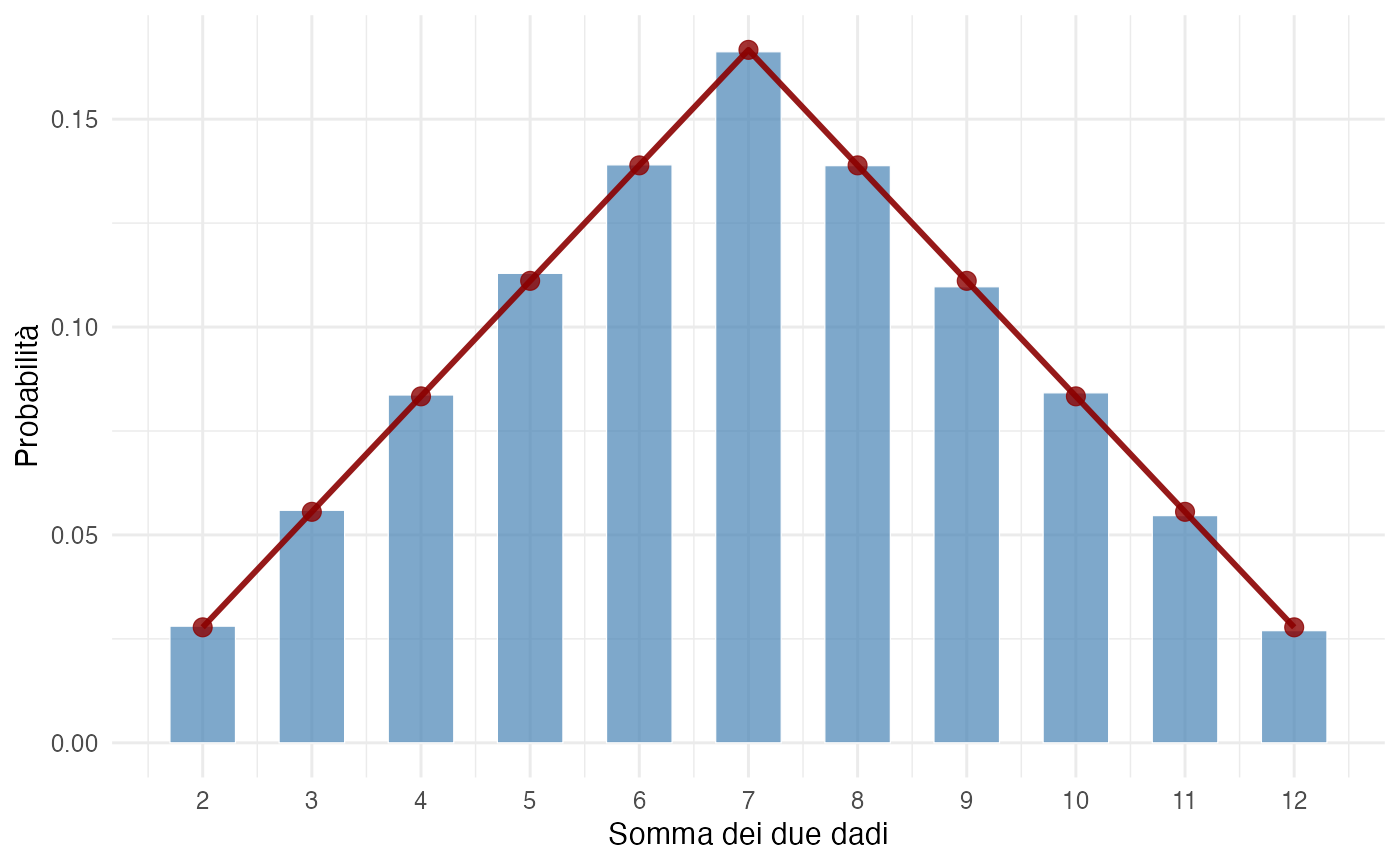
\includegraphics[width=0.85\linewidth,height=\textheight,keepaspectratio]{chapters/probability/06_random_var_files/figure-pdf/fig-pmf-dice-1.png}

}

\caption{\label{fig-pmf-dice}Confronto tra distribuzione teorica (linea)
e frequenze empiriche (barre) per la somma di due dadi. Con 100,000
simulazioni, la convergenza è evidente.}

\end{figure}%

La convergenza delle frequenze empiriche alle probabilità teoriche non
le definisce, ma ne verifica la coerenza, confermando che le nostre
assegnazioni di credenza producono il comportamento atteso quando
sottoposte a test ripetuti.

\section{Variabili casuali continue}\label{variabili-casuali-continue}

Molte grandezze psicologiche non possono essere rappresentate
adeguatamente da variabili discrete. Il tempo di reazione in un compito
cognitivo, il livello di cortisolo in una misurazione fisiologica, la
latenza di una risposta: tutte queste quantità possono assumere, almeno
in linea di principio, \textbf{qualsiasi} valore in un intervallo
continuo. Per questo motivo, introduciamo le variabili casuali continue.

\begin{definition}[Variabile casuale
continua]\protect\hypertarget{def-continuous-rv}{}\label{def-continuous-rv}

Una variabile casuale \(X\) è \emph{continua} se esiste una funzione non
negativa \(f_X : \mathbb{R} \to [0, +\infty)\), detta \emph{funzione di
densità di probabilità} (PDF), tale che per ogni intervallo \([a, b]\):
\[
P(a \leq X \leq b) = \int_a^b f_X(x) \, dx.
\]

\end{definition}

\subsection{Funzione di densità di
probabilità}\label{funzione-di-densituxe0-di-probabilituxe0}

La PDF ha per le variabili continue un ruolo analogo a quello della PMF
per le variabili discrete, ma con una differenza cruciale: \(f_X(x)\)
\emph{non} rappresenta la probabilità che \(X\) assuma il valore \(x\).
Infatti, per una variabile continua, la probabilità di assumere un
valore \emph{esatto} è sempre zero: \[
P(X = x_0) = \int_{x_0}^{x_0} f_X(x) \, dx = 0.
\]

Questo risultato, apparentemente controintuitivo, riflette il fatto che
in un continuum ci sono ``troppi'' punti perché ciascuno possa avere una
probabilità positiva, mantenendo la normalizzazione. La probabilità si
``distribuisce'' sull'intera retta reale e solo gli intervalli possono
avere una probabilità non nulla.

La densità \(f_X(x)\) può essere interpretata come una misura di
\emph{concentrazione} della probabilità: valori elevati di \(f_X(x)\)
indicano regioni in cui la variabile è più probabile che si verifichi,
nel senso che piccoli intervalli attorno a quei punti hanno una
probabilità relativamente alta.

\begin{theorem}[Proprietà delle funzioni di densità di
probabilità]\protect\hypertarget{thm-pdf-properties}{}\label{thm-pdf-properties}

Una funzione \(f_X(x)\) costituisce una valida funzione di densità di
probabilità se e solo se soddisfa le seguenti condizioni necessarie e
sufficienti:

\begin{itemize}
\item
  \textbf{non-negatività}: la funzione deve assumere valori non negativi
  su tutto il suo dominio, ovvero \(f_X(x) \geq 0\) per ogni
  \(x \in \mathbb{R}\). Questa proprietà garantisce che la probabilità
  associata a qualsiasi intervallo sia sempre non negativa.
\item
  \textbf{normalizzazione}: l'integrale della funzione esteso all'intero
  asse reale deve essere uguale a 1, formalmente
  \(\int_{-\infty}^{+\infty} f_X(x)  dx = 1\). Questa condizione
  garantisce che la probabilità totale dello spazio campionario sia
  unitaria, coerentemente con gli assiomi della probabilità.
\end{itemize}

\end{theorem}

Si noti che il valore della funzione di densità di probabilità
\(f_X(x)\) può superare l'unità, in quanto essa non rappresenta una
probabilità, bensì una densità di probabilità. Solo l'integrale di
questa funzione su un intervallo misurabile restituisce una probabilità
propriamente detta. Formalmente, la probabilità che la variabile casuale
\(X\) assuma valori nell'intervallo \([a,b]\) è data da
\(P(a \leq X \leq b) = \int_a^b f_X(x)  dx\), dove l'area sottesa dalla
curva nell'intervallo corrisponde alla probabilità dell'evento.

\begin{tcolorbox}[enhanced jigsaw, arc=.35mm, breakable, colbacktitle=quarto-callout-note-color!10!white, opacityback=0, toprule=.15mm, rightrule=.15mm, colback=white, opacitybacktitle=0.6, leftrule=.75mm, coltitle=black, bottomtitle=1mm, left=2mm, toptitle=1mm, title=\textcolor{quarto-callout-note-color}{\faInfo}\hspace{0.5em}{Esempio: tempo di reazione in un intervallo}, titlerule=0mm, bottomrule=.15mm, colframe=quarto-callout-note-color-frame]

Consideriamo una variabile casuale continua \(T\) che rappresenta il
tempo di reazione in un compito sperimentale. Supponiamo che \(T\) segua
una distribuzione log-normale con parametri \(\mu = 5.7\) e
\(\sigma = 0.3\). Ciò significa che il logaritmo naturale del tempo di
reazione, \(\ln(T)\), segue una distribuzione normale.

La sua funzione di densità di probabilità (PDF) è data da:

\[
f_T(t) = \frac{1}{t \sigma \sqrt{2\pi}} \exp\left(-\frac{(\ln(t) - \mu)^2}{2\sigma^2}\right) \quad \text{per } t > 0
\] e \(f_T(t) = 0\) per \(t \leq 0\).

\begin{Shaded}
\begin{Highlighting}[]
\CommentTok{\# Parametri della distribuzione log{-}normale}
\NormalTok{mu }\OtherTok{\textless{}{-}} \FloatTok{5.7}   \CommentTok{\# Parametro di location (media del log(T))}
\NormalTok{sigma }\OtherTok{\textless{}{-}} \FloatTok{0.3} \CommentTok{\# Parametro di scale (deviazione standard del log(T))}

\CommentTok{\# Calcolo di media e mediana della distribuzione originale}
\NormalTok{media\_T }\OtherTok{\textless{}{-}} \FunctionTok{exp}\NormalTok{(mu }\SpecialCharTok{+}\NormalTok{ sigma}\SpecialCharTok{\^{}}\DecValTok{2} \SpecialCharTok{/} \DecValTok{2}\NormalTok{)}
\NormalTok{mediana\_T }\OtherTok{\textless{}{-}} \FunctionTok{exp}\NormalTok{(mu)}
\end{Highlighting}
\end{Shaded}

\begin{verbatim}
#> Parametri per ln(T): µ = 5.7 , σ = 0.3
#> Mediana del tempo di reazione T: 299 ms
#> Media del tempo di reazione T: 313 ms
\end{verbatim}

Ora, calcoliamo la probabilità che il tempo di reazione sia compreso tra
300 e 400 millisecondi. Questo richiede di integrare la funzione di
densità in quell'intervallo.

\[
P(300 \leq T \leq 400) = \int_{300}^{400} f_T(t) \, dt .
\]

\begin{Shaded}
\begin{Highlighting}[]
\CommentTok{\# Calcolo della probabilità tra 300 e 400 ms usando la CDF}
\NormalTok{prob\_300\_400 }\OtherTok{\textless{}{-}} \FunctionTok{plnorm}\NormalTok{(}\DecValTok{400}\NormalTok{, }\AttributeTok{meanlog =}\NormalTok{ mu, }\AttributeTok{sdlog =}\NormalTok{ sigma) }\SpecialCharTok{{-}} \FunctionTok{plnorm}\NormalTok{(}\DecValTok{300}\NormalTok{, }\AttributeTok{meanlog =}\NormalTok{ mu, }\AttributeTok{sdlog =}\NormalTok{ sigma)}
\end{Highlighting}
\end{Shaded}

\begin{verbatim}
#> Probabilità P(300 ≤ T ≤ 400): 0.329
\end{verbatim}

Verifichiamo la proprietà fondamentale di normalizzazione, che
garantisce che la probabilità totale su tutti i tempi di reazione
possibili sia uguale a 1.

\[
\int_{0}^{\infty} f_T(t) \, dt = 1.
\]

\begin{Shaded}
\begin{Highlighting}[]
\CommentTok{\# Verifica della normalizzazione (la CDF a +infinito deve essere 1)}
\NormalTok{prob\_totale }\OtherTok{\textless{}{-}} \FunctionTok{plnorm}\NormalTok{(}\ConstantTok{Inf}\NormalTok{, }\AttributeTok{meanlog =}\NormalTok{ mu, }\AttributeTok{sdlog =}\NormalTok{ sigma)}
\end{Highlighting}
\end{Shaded}

\begin{verbatim}
#> Verifica normalizzazione [P(0 < T < ∞)]: 1 -> ✓ OK
\end{verbatim}

\textbf{Calcoli aggiuntivi per comprendere la forma della
distribuzione:}

\begin{Shaded}
\begin{Highlighting}[]
\CommentTok{\# Calcolo di altri intervalli probabilistici di interesse}
\FunctionTok{cat}\NormalTok{(}\StringTok{"}\SpecialCharTok{\textbackslash{}n}\StringTok{Probabilità per altri intervalli:}\SpecialCharTok{\textbackslash{}n}\StringTok{"}\NormalTok{)}
\CommentTok{\#\textgreater{} }
\CommentTok{\#\textgreater{} Probabilità per altri intervalli:}
\FunctionTok{cat}\NormalTok{(}\StringTok{"P(T ≤ 250 ms):"}\NormalTok{, }\FunctionTok{round}\NormalTok{(}\FunctionTok{plnorm}\NormalTok{(}\DecValTok{250}\NormalTok{, mu, sigma), }\DecValTok{3}\NormalTok{), }\StringTok{"}\SpecialCharTok{\textbackslash{}n}\StringTok{"}\NormalTok{)}
\CommentTok{\#\textgreater{} P(T ≤ 250 ms): 0.276}
\FunctionTok{cat}\NormalTok{(}\StringTok{"P(T ≥ 500 ms):"}\NormalTok{, }\FunctionTok{round}\NormalTok{(}\DecValTok{1} \SpecialCharTok{{-}} \FunctionTok{plnorm}\NormalTok{(}\DecValTok{500}\NormalTok{, mu, sigma), }\DecValTok{3}\NormalTok{), }\StringTok{"}\SpecialCharTok{\textbackslash{}n}\StringTok{"}\NormalTok{)}
\CommentTok{\#\textgreater{} P(T ≥ 500 ms): 0.043}
\FunctionTok{cat}\NormalTok{(}\StringTok{"P(T tra mediana e media):"}\NormalTok{, }\FunctionTok{round}\NormalTok{(}\FunctionTok{plnorm}\NormalTok{(media\_T, mu, sigma) }\SpecialCharTok{{-}} \FunctionTok{plnorm}\NormalTok{(mediana\_T, mu, sigma), }\DecValTok{3}\NormalTok{), }\StringTok{"}\SpecialCharTok{\textbackslash{}n}\StringTok{"}\NormalTok{)}
\CommentTok{\#\textgreater{} P(T tra mediana e media): 0.06}
\end{Highlighting}
\end{Shaded}

\begin{Shaded}
\begin{Highlighting}[]
\CommentTok{\# Intervallo che cattura il 95\% della distribuzione}
\NormalTok{intervallo\_95 }\OtherTok{\textless{}{-}} \FunctionTok{qlnorm}\NormalTok{(}\FunctionTok{c}\NormalTok{(}\FloatTok{0.025}\NormalTok{, }\FloatTok{0.975}\NormalTok{), }\AttributeTok{meanlog =}\NormalTok{ mu, }\AttributeTok{sdlog =}\NormalTok{ sigma)}
\end{Highlighting}
\end{Shaded}

\begin{verbatim}
#> 
#> Intervallo centrale al 95% per T: [166, 538] ms
\end{verbatim}

\end{tcolorbox}

\section{Funzione di distribuzione
cumulativa}\label{funzione-di-distribuzione-cumulativa}

Esiste una descrizione alternativa, valida sia per variabili discrete
che continue, che specifica la probabilità che la variabile assuma
valori inferiori o uguali a un determinato livello soglia.

\begin{definition}[Funzione di distribuzione cumulativa
(CDF)]\protect\hypertarget{def-cdf}{}\label{def-cdf}

La \emph{funzione di ripartizione} (o funzione di distribuzione
cumulativa) di una variabile casuale \(X\) è la funzione
\(F_X : \mathbb{R} \to [0,1]\) definita da \[
F_X(x) = P(X \leq x).
\]

\end{definition}

La funzione di ripartizione fornisce una caratterizzazione completa
della distribuzione di probabilità di \(X\). Da essa è possibile
ricavare la funzione di massa di probabilità per le variabili discrete o
la funzione di densità di probabilità per le variabili continue e
viceversa. Per le variabili continue, sussiste la relazione: \[
F_X(x) = \int_{-\infty}^{x} f_X(t) \, dt, \qquad f_X(x) = \frac{d}{dx} F_X(x).
\]

\begin{theorem}[Proprietà della funzione di
ripartizione]\protect\hypertarget{thm-cdf-properties}{}\label{thm-cdf-properties}

Ogni funzione di ripartizione soddisfa le seguenti proprietà
fondamentali:

\begin{enumerate}
\def\labelenumi{\arabic{enumi}.}
\tightlist
\item
  \textbf{Monotonia non decrescente}: per ogni coppia \(a < b\), risulta
  \(F_X(a) \leq F_X(b)\).
\item
  \textbf{Comportamento asintotico}: \(\lim_{x \to -\infty} F_X(x) = 0\)
  e \(\lim_{x \to +\infty} F_X(x) = 1\).
\item
  \textbf{Continuità da destra}:
  \(\lim_{h \to 0^+} F_X(x + h) = F_X(x)\) per ogni
  \(x \in \mathbb{R}\).
\end{enumerate}

\end{theorem}

La proprietà di monotonia riflette il fatto che, estendendo l'intervallo
\((-\infty, x]\) verso destra, la probabilità cumulata non può
diminuire. I limiti asintotici garantiscono la corretta normalizzazione
della probabilità totale. La continuità da destra è una convenzione
matematica che risolve le ambiguità nel caso di variabili discrete.

Per le variabili continue, la funzione di ripartizione risulta continua
su tutto il suo dominio, mentre per le variabili discrete presenta
discontinuità di prima specie nei punti corrispondenti ai valori assunti
con probabilità positiva.

\begin{Shaded}
\begin{Highlighting}[]
\CommentTok{\# CDF teorica per la somma di due dadi}
\NormalTok{valori }\OtherTok{\textless{}{-}} \DecValTok{2}\SpecialCharTok{:}\DecValTok{12}
\NormalTok{prob }\OtherTok{\textless{}{-}} \FunctionTok{c}\NormalTok{(}\DecValTok{1}\NormalTok{, }\DecValTok{2}\NormalTok{, }\DecValTok{3}\NormalTok{, }\DecValTok{4}\NormalTok{, }\DecValTok{5}\NormalTok{, }\DecValTok{6}\NormalTok{, }\DecValTok{5}\NormalTok{, }\DecValTok{4}\NormalTok{, }\DecValTok{3}\NormalTok{, }\DecValTok{2}\NormalTok{, }\DecValTok{1}\NormalTok{) }\SpecialCharTok{/} \DecValTok{36}
\NormalTok{cdf }\OtherTok{\textless{}{-}} \FunctionTok{cumsum}\NormalTok{(prob)}

\CommentTok{\# Creiamo i dati per il grafico a gradini}
\NormalTok{df\_cdf }\OtherTok{\textless{}{-}} \FunctionTok{data.frame}\NormalTok{(}
  \AttributeTok{x\_start =} \FunctionTok{c}\NormalTok{(}\DecValTok{1}\NormalTok{, valori),}
  \AttributeTok{x\_end =} \FunctionTok{c}\NormalTok{(valori, }\DecValTok{13}\NormalTok{),}
  \AttributeTok{y =} \FunctionTok{c}\NormalTok{(}\DecValTok{0}\NormalTok{, cdf)}
\NormalTok{)}

\FunctionTok{ggplot}\NormalTok{() }\SpecialCharTok{+}
  \FunctionTok{geom\_segment}\NormalTok{(}\AttributeTok{data =}\NormalTok{ df\_cdf, }
               \FunctionTok{aes}\NormalTok{(}\AttributeTok{x =}\NormalTok{ x\_start, }\AttributeTok{xend =}\NormalTok{ x\_end, }\AttributeTok{y =}\NormalTok{ y, }\AttributeTok{yend =}\NormalTok{ y),}
               \AttributeTok{linewidth =} \DecValTok{1}\NormalTok{, }\AttributeTok{color =} \StringTok{"steelblue"}\NormalTok{) }\SpecialCharTok{+}
  \FunctionTok{geom\_point}\NormalTok{(}\AttributeTok{data =} \FunctionTok{data.frame}\NormalTok{(}\AttributeTok{x =}\NormalTok{ valori, }\AttributeTok{y =}\NormalTok{ cdf), }
             \FunctionTok{aes}\NormalTok{(}\AttributeTok{x =}\NormalTok{ x, }\AttributeTok{y =}\NormalTok{ y), }
             \AttributeTok{size =} \DecValTok{3}\NormalTok{, }\AttributeTok{color =} \StringTok{"steelblue"}\NormalTok{) }\SpecialCharTok{+}
  \FunctionTok{scale\_x\_continuous}\NormalTok{(}\AttributeTok{breaks =} \DecValTok{2}\SpecialCharTok{:}\DecValTok{12}\NormalTok{, }\AttributeTok{limits =} \FunctionTok{c}\NormalTok{(}\DecValTok{1}\NormalTok{, }\DecValTok{13}\NormalTok{)) }\SpecialCharTok{+}
  \FunctionTok{scale\_y\_continuous}\NormalTok{(}\AttributeTok{breaks =} \FunctionTok{seq}\NormalTok{(}\DecValTok{0}\NormalTok{, }\DecValTok{1}\NormalTok{, }\FloatTok{0.2}\NormalTok{)) }\SpecialCharTok{+}
  \FunctionTok{labs}\NormalTok{(}\AttributeTok{x =} \StringTok{"x"}\NormalTok{, }\AttributeTok{y =} \FunctionTok{expression}\NormalTok{(F[X](x) }\SpecialCharTok{==} \FunctionTok{P}\NormalTok{(X }\SpecialCharTok{\textless{}=}\NormalTok{ x))) }\SpecialCharTok{+}
  \FunctionTok{theme\_minimal}\NormalTok{()}
\end{Highlighting}
\end{Shaded}

\begin{figure}[H]

\centering{

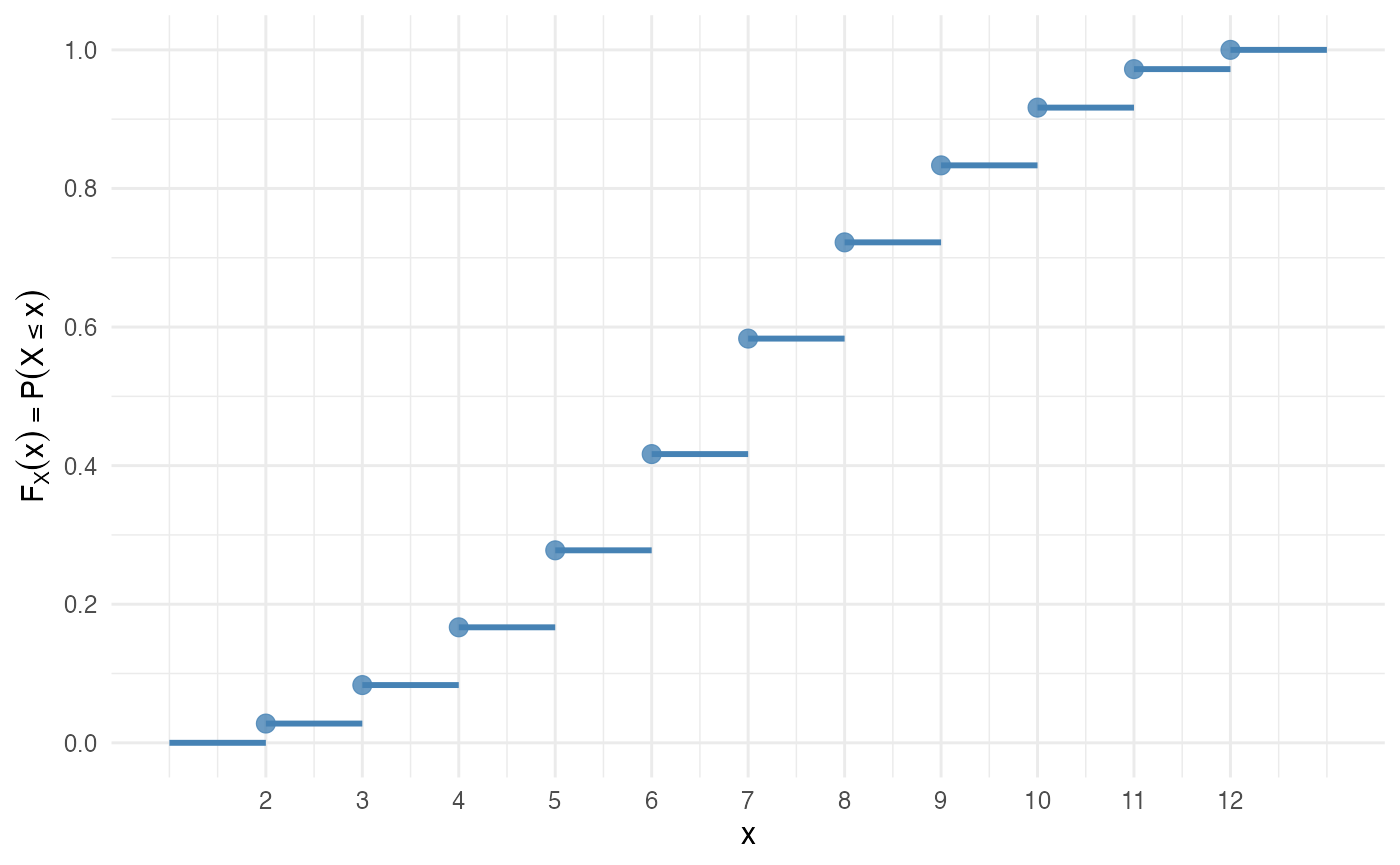
\includegraphics[width=0.85\linewidth,height=\textheight,keepaspectratio]{chapters/probability/06_random_var_files/figure-pdf/fig-cdf-dice-1.png}

}

\caption{\label{fig-cdf-dice}CDF della somma di due dadi. I salti
corrispondono ai valori possibili, e l'altezza di ogni salto è pari alla
probabilità di quel valore.}

\end{figure}%

\section{Variabili casuali multiple}\label{variabili-casuali-multiple}

In numerosi contesti sperimentali, risulta necessario modellare
simultaneamente più fenomeni aleatori. Ad esempio, in uno studio
psicometrico che indaga la relazione tra ansia e depressione, potrebbe
essere necessario rappresentare congiuntamente i punteggi di entrambi i
costrutti. Il framework probabilistico si estende naturalmente a questo
scenario multivariato.

\begin{definition}[Distribuzione
congiunta]\protect\hypertarget{def-joint-distribution}{}\label{def-joint-distribution}

Per due variabili casuali discrete \(X\) e \(Y\), la \emph{funzione di
massa di probabilità congiunta} è definita come: \[
p_{X,Y}(x, y) = P(X = x, Y = y).
\]

Le corrispondenti \emph{distribuzioni marginali} si ottengono mediante
la somma sulle variabili non interessate: \[
p_X(x) = \sum_y p_{X,Y}(x, y), \qquad p_Y(y) = \sum_x p_{X,Y}(x, y).
\]

\end{definition}

Le variabili \(X\) e \(Y\) si dicono \emph{stocasticamente indipendenti}
se e solo se \(p_{X,Y}(x, y) = p_X(x) \cdot p_Y(y)\) per ogni coppia di
valori \((x, y)\). L'indipendenza implica che l'informazione sul valore
assunto da una variabile non modifichi la distribuzione di probabilità
dell'altra.

\section*{Riflessioni conclusive}\label{riflessioni-conclusive-5}

\markright{Riflessioni conclusive}

Il concetto di variabile casuale rappresenta il ponte fondamentale tra
la teoria della probabilità, intesa come sistema di credenze coerenti, e
l'analisi quantitativa dei fenomeni incerti. Attraverso questa
formalizzazione, è possibile tradurre qualsiasi risultato sperimentale,
di natura qualitativa o quantitativa, in un oggetto matematico
suscettibile di essere trattato con gli strumenti del calcolo delle
probabilità.

Le due grandi classi di variabili casuali, discrete e continue,
richiedono formalizzazioni distinte, ma concettualmente omogenee. La
funzione di massa di probabilità (PMF) per le variabili discrete e la
funzione di densità di probabilità (PDF) per quelle continue svolgono un
ruolo analogo nel caratterizzare la distribuzione della probabilità
nello spazio dei possibili valori. La funzione di ripartizione (CDF)
fornisce invece una rappresentazione unificante applicabile a entrambe
le tipologie.

Il valore atteso e la varianza sono gli strumenti principali per
sintetizzare le caratteristiche distributive. Il valore atteso localizza
il baricentro probabilistico della distribuzione, mentre la varianza ne
quantifica la dispersione attorno a tale centro. Le proprietà algebriche
di questi operatori, in particolare la linearità del valore atteso e
l'additività della varianza per variabili indipendenti, costituiscono
strumenti di notevole efficacia per semplificare i calcoli applicativi.

Questi fondamenti troveranno immediata applicazione nei capitoli
successivi, dedicati allo studio di specifiche famiglie parametriche di
distribuzioni (Beta, Normale, Poisson e Binomiale), che rappresentano i
costituenti elementari della modellazione statistica bayesiana. Le
distribuzioni a priori, le funzioni di verosimiglianza e le
distribuzioni a posteriori, i tre pilastri concettuali dell'inferenza
bayesiana, trovano infatti piena espressione nel linguaggio delle
variabili casuali qui introdotto.

\begin{tcolorbox}[enhanced jigsaw, arc=.35mm, breakable, colbacktitle=quarto-callout-note-color!10!white, opacityback=0, toprule=.15mm, rightrule=.15mm, colback=white, opacitybacktitle=0.6, leftrule=.75mm, coltitle=black, bottomtitle=1mm, left=2mm, toptitle=1mm, title=\textcolor{quarto-callout-note-color}{\faInfo}\hspace{0.5em}{Informazioni sull'ambiente di sviluppo}, titlerule=0mm, bottomrule=.15mm, colframe=quarto-callout-note-color-frame]

\begin{Shaded}
\begin{Highlighting}[]
\FunctionTok{sessionInfo}\NormalTok{()}
\CommentTok{\#\textgreater{} R version 4.5.2 (2025{-}10{-}31)}
\CommentTok{\#\textgreater{} Platform: aarch64{-}apple{-}darwin20}
\CommentTok{\#\textgreater{} Running under: macOS Tahoe 26.1}
\CommentTok{\#\textgreater{} }
\CommentTok{\#\textgreater{} Matrix products: default}
\CommentTok{\#\textgreater{} BLAS:   /System/Library/Frameworks/Accelerate.framework/Versions/A/Frameworks/vecLib.framework/Versions/A/libBLAS.dylib }
\CommentTok{\#\textgreater{} LAPACK: /Library/Frameworks/R.framework/Versions/4.5{-}arm64/Resources/lib/libRlapack.dylib;  LAPACK version 3.12.1}
\CommentTok{\#\textgreater{} }
\CommentTok{\#\textgreater{} locale:}
\CommentTok{\#\textgreater{} [1] C.UTF{-}8/UTF{-}8/C.UTF{-}8/C/C.UTF{-}8/C.UTF{-}8}
\CommentTok{\#\textgreater{} }
\CommentTok{\#\textgreater{} time zone: Europe/Rome}
\CommentTok{\#\textgreater{} tzcode source: internal}
\CommentTok{\#\textgreater{} }
\CommentTok{\#\textgreater{} attached base packages:}
\CommentTok{\#\textgreater{} [1] stats     graphics  grDevices utils     datasets  methods   base     }
\CommentTok{\#\textgreater{} }
\CommentTok{\#\textgreater{} other attached packages:}
\CommentTok{\#\textgreater{}  [1] pillar\_1.11.1         tinytable\_0.15.1      patchwork\_1.3.2      }
\CommentTok{\#\textgreater{}  [4] ggdist\_3.3.3          tidybayes\_3.0.7       bayesplot\_1.14.0     }
\CommentTok{\#\textgreater{}  [7] ggplot2\_4.0.1         reliabilitydiag\_0.2.1 priorsense\_1.2.0     }
\CommentTok{\#\textgreater{} [10] posterior\_1.6.1       loo\_2.8.0             rstan\_2.32.7         }
\CommentTok{\#\textgreater{} [13] StanHeaders\_2.32.10   brms\_2.23.0           Rcpp\_1.1.0           }
\CommentTok{\#\textgreater{} [16] sessioninfo\_1.2.3     conflicted\_1.2.0      janitor\_2.2.1        }
\CommentTok{\#\textgreater{} [19] matrixStats\_1.5.0     modelr\_0.1.11         tibble\_3.3.0         }
\CommentTok{\#\textgreater{} [22] dplyr\_1.1.4           tidyr\_1.3.1           rio\_1.2.4            }
\CommentTok{\#\textgreater{} [25] here\_1.0.2           }
\CommentTok{\#\textgreater{} }
\CommentTok{\#\textgreater{} loaded via a namespace (and not attached):}
\CommentTok{\#\textgreater{}  [1] svUnit\_1.0.8          tidyselect\_1.2.1      farver\_2.1.2         }
\CommentTok{\#\textgreater{}  [4] S7\_0.2.1              fastmap\_1.2.0         TH.data\_1.1{-}5        }
\CommentTok{\#\textgreater{}  [7] tensorA\_0.36.2.1      pacman\_0.5.1          digest\_0.6.39        }
\CommentTok{\#\textgreater{} [10] timechange\_0.3.0      estimability\_1.5.1    lifecycle\_1.0.4      }
\CommentTok{\#\textgreater{} [13] survival\_3.8{-}3        magrittr\_2.0.4        compiler\_4.5.2       }
\CommentTok{\#\textgreater{} [16] rlang\_1.1.6           tools\_4.5.2           yaml\_2.3.10          }
\CommentTok{\#\textgreater{} [19] knitr\_1.50            labeling\_0.4.3        bridgesampling\_1.2{-}1 }
\CommentTok{\#\textgreater{} [22] curl\_7.0.0            pkgbuild\_1.4.8        RColorBrewer\_1.1{-}3   }
\CommentTok{\#\textgreater{} [25] abind\_1.4{-}8           multcomp\_1.4{-}29       withr\_3.0.2          }
\CommentTok{\#\textgreater{} [28] purrr\_1.2.0           grid\_4.5.2            stats4\_4.5.2         }
\CommentTok{\#\textgreater{} [31] colorspace\_2.1{-}2      xtable\_1.8{-}4          inline\_0.3.21        }
\CommentTok{\#\textgreater{} [34] emmeans\_2.0.0         scales\_1.4.0          MASS\_7.3{-}65          }
\CommentTok{\#\textgreater{} [37] cli\_3.6.5             mvtnorm\_1.3{-}3         rmarkdown\_2.30       }
\CommentTok{\#\textgreater{} [40] ragg\_1.5.0            generics\_0.1.4        RcppParallel\_5.1.11{-}1}
\CommentTok{\#\textgreater{} [43] cachem\_1.1.0          stringr\_1.6.0         splines\_4.5.2        }
\CommentTok{\#\textgreater{} [46] parallel\_4.5.2        vctrs\_0.6.5           V8\_8.0.1             }
\CommentTok{\#\textgreater{} [49] Matrix\_1.7{-}4          sandwich\_3.1{-}1        jsonlite\_2.0.0       }
\CommentTok{\#\textgreater{} [52] arrayhelpers\_1.1{-}0    systemfonts\_1.3.1     glue\_1.8.0           }
\CommentTok{\#\textgreater{} [55] codetools\_0.2{-}20      distributional\_0.5.0  lubridate\_1.9.4      }
\CommentTok{\#\textgreater{} [58] stringi\_1.8.7         gtable\_0.3.6          QuickJSR\_1.8.1       }
\CommentTok{\#\textgreater{} [61] htmltools\_0.5.8.1     Brobdingnag\_1.2{-}9     R6\_2.6.1             }
\CommentTok{\#\textgreater{} [64] textshaping\_1.0.4     rprojroot\_2.1.1       evaluate\_1.0.5       }
\CommentTok{\#\textgreater{} [67] lattice\_0.22{-}7        backports\_1.5.0       memoise\_2.0.1        }
\CommentTok{\#\textgreater{} [70] broom\_1.0.10          snakecase\_0.11.1      rstantools\_2.5.0     }
\CommentTok{\#\textgreater{} [73] coda\_0.19{-}4.1         gridExtra\_2.3         nlme\_3.1{-}168         }
\CommentTok{\#\textgreater{} [76] checkmate\_2.3.3       xfun\_0.54             zoo\_1.8{-}14           }
\CommentTok{\#\textgreater{} [79] pkgconfig\_2.0.3}
\end{Highlighting}
\end{Shaded}

\end{tcolorbox}

\section*{Bibliografia}\label{bibliografia-3}

\markright{Bibliografia}

\chapter{Distribuzioni di massa e di densità}\label{sec-prob-distr}

\section*{Introduzione}\label{introduzione-7}

\markright{Introduzione}

Nel Chapter~\ref{sec-prob-random-var} abbiamo introdotto le variabili
casuali come funzioni che traducono gli esiti di un esperimento
aleatorio in valori numerici. Abbiamo distinto le variabili discrete,
che assumono un insieme numerabile di valori, dalle variabili continue,
che possono assumere qualsiasi valore in un intervallo. Per ciascuna di
queste tipologie, abbiamo definito formalmente la funzione di massa di
probabilità (PMF) e la funzione di densità di probabilità (PDF).

Questo capitolo approfondisce la comprensione intuitiva di questi
concetti, esplorando il loro significato geometrico e operativo. Vedremo
come la funzione di massa di probabilità (PMF) assegni ``pesi'' discreti
ai singoli valori, mentre la funzione di densità di probabilità (PDF)
distribuisca la probabilità in modo continuo e richieda l'integrazione
per calcolare le probabilità su intervalli. Affronteremo anche il famoso
``paradosso'' per cui la probabilità di osservare un valore esatto in
una distribuzione continua è sempre pari a zero, mostrando come questa
proprietà, lungi dall'essere paradossale, emerga naturalmente dalla
struttura matematica del continuo.

Un aspetto centrale della trattazione riguarda la distinzione tra
l'interpretazione frequentista e quella bayesiana delle distribuzioni di
probabilità. Nel paradigma frequentista, la PDF descrive la
distribuzione dei dati in ipotetiche ripetizioni dell'esperimento,
mentre nell'approccio bayesiano essa quantifica il nostro grado di
credenza sui possibili valori di una quantità incerta. Questa
distinzione concettuale, apparentemente sottile, ha profonde
implicazioni per la pratica dell'inferenza statistica.

\subsection*{Panoramica del capitolo}\label{panoramica-del-capitolo-6}

\begin{itemize}
\tightlist
\item
  Distinzione operativa tra massa di probabilità e densità di
  probabilità.
\item
  Dagli istogrammi alle funzioni di densità: il limite continuo.
\item
  Il ``paradosso'' della probabilità zero per valori esatti.
\item
  La funzione di distribuzione cumulativa come rappresentazione
  unificata.
\item
  Interpretazioni bayesiana e frequentista delle distribuzioni.
\end{itemize}

\begin{tcolorbox}[enhanced jigsaw, arc=.35mm, breakable, colbacktitle=quarto-callout-tip-color!10!white, opacityback=0, toprule=.15mm, rightrule=.15mm, colback=white, opacitybacktitle=0.6, leftrule=.75mm, coltitle=black, bottomtitle=1mm, left=2mm, toptitle=1mm, title=\textcolor{quarto-callout-tip-color}{\faLightbulb}\hspace{0.5em}{Prerequisiti}, titlerule=0mm, bottomrule=.15mm, colframe=quarto-callout-tip-color-frame]

\begin{itemize}
\tightlist
\item
  Aver letto il Chapter~\ref{sec-prob-random-var} sulle variabili
  casuali.
\item
  Familiarità con il concetto di integrale come area sotto una curva.
\item
  Leggere il capitolo \emph{Random variables and their distributions} di
  Blitzstein \& Hwang (\citeproc{ref-blitzstein2019introduction}{2019}).
\end{itemize}

\end{tcolorbox}

\begin{tcolorbox}[enhanced jigsaw, arc=.35mm, breakable, colbacktitle=quarto-callout-caution-color!10!white, opacityback=0, toprule=.15mm, rightrule=.15mm, colback=white, opacitybacktitle=0.6, leftrule=.75mm, coltitle=black, bottomtitle=1mm, left=2mm, toptitle=1mm, title=\textcolor{quarto-callout-caution-color}{\faFire}\hspace{0.5em}{Preparazione del Notebook}, titlerule=0mm, bottomrule=.15mm, colframe=quarto-callout-caution-color-frame]

\begin{Shaded}
\begin{Highlighting}[]
\NormalTok{here}\SpecialCharTok{::}\FunctionTok{here}\NormalTok{(}\StringTok{"code"}\NormalTok{, }\StringTok{"\_common.R"}\NormalTok{) }\SpecialCharTok{|\textgreater{}} 
  \FunctionTok{source}\NormalTok{()}

\CommentTok{\# Pacchetti necessari}
\ControlFlowTok{if}\NormalTok{ (}\SpecialCharTok{!}\FunctionTok{requireNamespace}\NormalTok{(}\StringTok{"pacman"}\NormalTok{)) }\FunctionTok{install.packages}\NormalTok{(}\StringTok{"pacman"}\NormalTok{)}
\NormalTok{pacman}\SpecialCharTok{::}\FunctionTok{p\_load}\NormalTok{(ggplot2, dplyr, tidyr)}
\end{Highlighting}
\end{Shaded}

\end{tcolorbox}

\section{Dalla massa alla densità di
probabilità}\label{dalla-massa-alla-densituxe0-di-probabilituxe0}

La distinzione tra variabili casuali discrete e continue non è meramente
tecnica, ma riflette una differenza fondamentale nel modo in cui la
probabilità si distribuisce sui possibili valori. Per le variabili
discrete, è possibile assegnare una probabilità positiva a ciascun
valore, mentre per le variabili continue, la probabilità si ``spalma''
su un continuum e solo gli intervalli possono avere una probabilità non
nulla.

\subsection{La funzione di massa di
probabilità}\label{la-funzione-di-massa-di-probabilituxe0}

Per una variabile casuale discreta \(X\) che assume valori nell'insieme
\(\mathcal{X} = \{x_1, x_2, \ldots\}\), la funzione di massa di
probabilità (PMF) associa a ciascun valore la corrispondente
probabilità: \[
p_X(x) = P(X = x).
\]

Il termine ``massa'' evoca l'immagine fisica di pesi discreti
posizionati sui valori possibili: ogni valore \(x_i\) è associato a un
``peso'' \(p_X(x_i)\), e la somma di tutti i pesi deve essere pari a 1.
Questa metafora è particolarmente appropriata, perché, come in fisica, è
possibile ``concentrare'' la probabilità in punti specifici.

\begin{tcolorbox}[enhanced jigsaw, arc=.35mm, breakable, colbacktitle=quarto-callout-note-color!10!white, opacityback=0, toprule=.15mm, rightrule=.15mm, colback=white, opacitybacktitle=0.6, leftrule=.75mm, coltitle=black, bottomtitle=1mm, left=2mm, toptitle=1mm, title=\textcolor{quarto-callout-note-color}{\faInfo}\hspace{0.5em}{Esempio: Dado sbilanciato}, titlerule=0mm, bottomrule=.15mm, colframe=quarto-callout-note-color-frame]

\subsection*{Distribuzione non
uniforme}\label{distribuzione-non-uniforme}

Consideriamo un dado truccato con la seguente distribuzione di
probabilità:

\begin{longtable}[]{@{}ccccccc@{}}
\toprule\noalign{}
Faccia & 1 & 2 & 3 & 4 & 5 & 6 \\
\midrule\noalign{}
\endhead
\bottomrule\noalign{}
\endlastfoot
\(p_X(x)\) & 0.10 & 0.15 & 0.20 & 0.25 & 0.20 & 0.10 \\
\end{longtable}

Questa PMF assegna probabilità maggiore ai valori centrali (3, 4, 5)
rispetto a quelli estremi (1, 6). Possiamo verificare la coerenza:
\(\sum_{x=1}^{6} p_X(x) = 0.10 + 0.15 + 0.20 + 0.25 + 0.20 + 0.10 = 1.00\).

Simuliamo 10,000 lanci di questo dado e confrontiamo le frequenze
empiriche con la PMF teorica:

\begin{Shaded}
\begin{Highlighting}[]
\FunctionTok{set.seed}\NormalTok{(}\DecValTok{123}\NormalTok{)}
\NormalTok{prob\_teoriche }\OtherTok{\textless{}{-}} \FunctionTok{c}\NormalTok{(}\FloatTok{0.10}\NormalTok{, }\FloatTok{0.15}\NormalTok{, }\FloatTok{0.20}\NormalTok{, }\FloatTok{0.25}\NormalTok{, }\FloatTok{0.20}\NormalTok{, }\FloatTok{0.10}\NormalTok{)}
\NormalTok{n\_lanci }\OtherTok{\textless{}{-}} \DecValTok{10000}

\CommentTok{\# Simulazione}
\NormalTok{lanci }\OtherTok{\textless{}{-}} \FunctionTok{sample}\NormalTok{(}\DecValTok{1}\SpecialCharTok{:}\DecValTok{6}\NormalTok{, }\AttributeTok{size =}\NormalTok{ n\_lanci, }\AttributeTok{replace =} \ConstantTok{TRUE}\NormalTok{, }\AttributeTok{prob =}\NormalTok{ prob\_teoriche)}

\CommentTok{\# Calcolo frequenze relative}
\NormalTok{freq\_rel }\OtherTok{\textless{}{-}} \FunctionTok{table}\NormalTok{(lanci) }\SpecialCharTok{/}\NormalTok{ n\_lanci}

\CommentTok{\# Dataframe per il grafico}
\NormalTok{df }\OtherTok{\textless{}{-}} \FunctionTok{data.frame}\NormalTok{(}
  \AttributeTok{valore =} \DecValTok{1}\SpecialCharTok{:}\DecValTok{6}\NormalTok{,}
  \AttributeTok{empirica =} \FunctionTok{as.numeric}\NormalTok{(freq\_rel),}
  \AttributeTok{teorica =}\NormalTok{ prob\_teoriche}
\NormalTok{)}

\FunctionTok{ggplot}\NormalTok{(df, }\FunctionTok{aes}\NormalTok{(}\AttributeTok{x =} \FunctionTok{factor}\NormalTok{(valore))) }\SpecialCharTok{+}
  \FunctionTok{geom\_col}\NormalTok{(}\FunctionTok{aes}\NormalTok{(}\AttributeTok{y =}\NormalTok{ empirica), }\AttributeTok{fill =} \StringTok{"steelblue"}\NormalTok{, }\AttributeTok{alpha =} \FloatTok{0.7}\NormalTok{, }\AttributeTok{width =} \FloatTok{0.6}\NormalTok{) }\SpecialCharTok{+}
  \FunctionTok{geom\_point}\NormalTok{(}\FunctionTok{aes}\NormalTok{(}\AttributeTok{y =}\NormalTok{ teorica), }\AttributeTok{color =} \StringTok{"darkred"}\NormalTok{, }\AttributeTok{size =} \DecValTok{4}\NormalTok{) }\SpecialCharTok{+}
  \FunctionTok{labs}\NormalTok{(}\AttributeTok{x =} \StringTok{"Faccia del dado"}\NormalTok{, }\AttributeTok{y =} \StringTok{"Probabilità / Frequenza relativa"}\NormalTok{) }\SpecialCharTok{+}
  \FunctionTok{theme\_minimal}\NormalTok{()}
\end{Highlighting}
\end{Shaded}

\begin{figure}[H]

\centering{

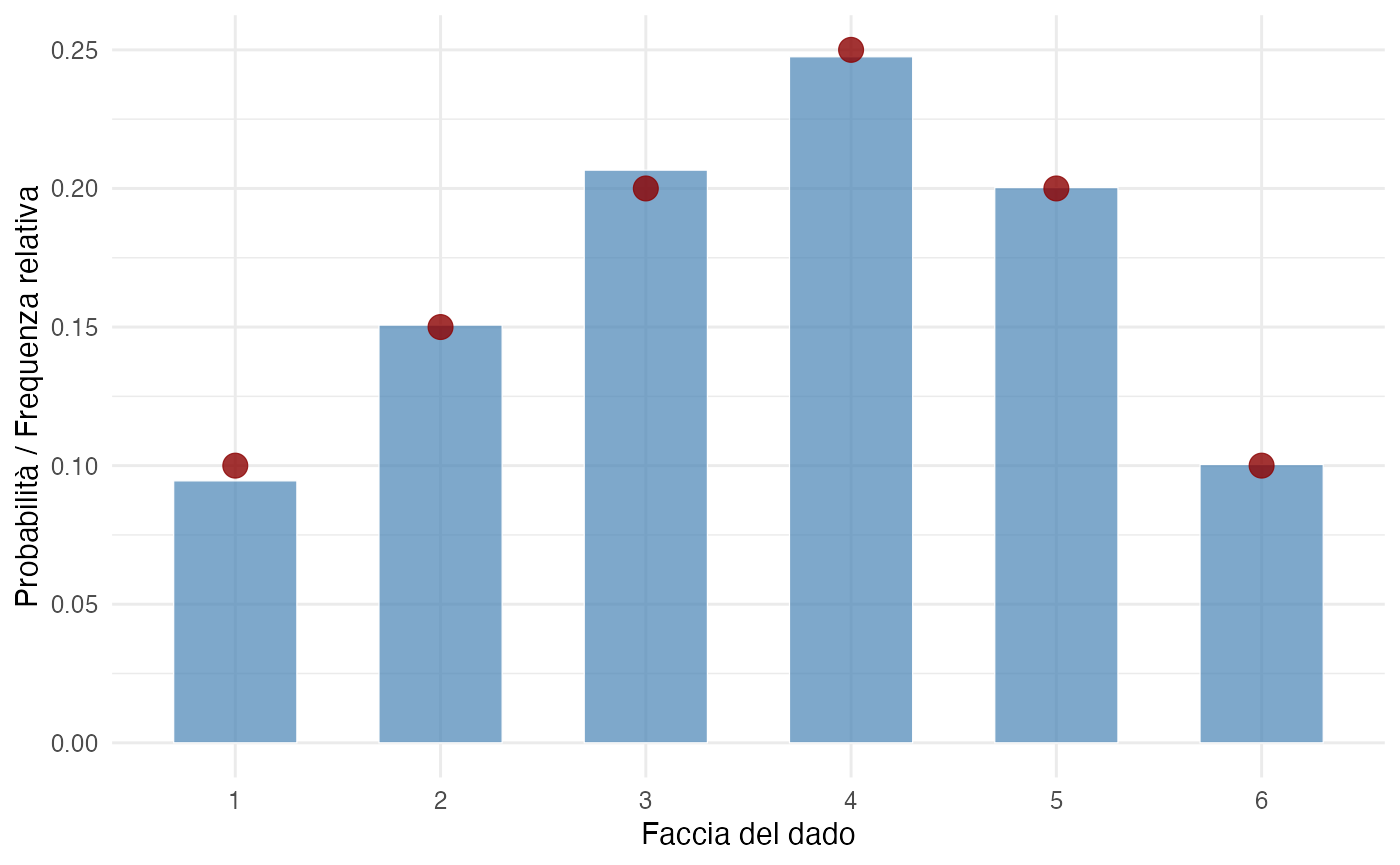
\includegraphics[width=0.85\linewidth,height=\textheight,keepaspectratio]{chapters/probability/07_prob_distributions_files/figure-pdf/fig-pmf-biased-die-1.png}

}

\caption{\label{fig-pmf-biased-die}Confronto tra PMF teorica (punti
rossi) e frequenze relative empiriche (barre) per un dado sbilanciato.
La convergenza illustra la coerenza tra credenze e comportamento
osservato.}

\end{figure}%

La convergenza delle frequenze empiriche alle probabilità teoriche non
definisce queste ultime, ma ne verifica la coerenza: le nostre
assegnazioni di credenza generano esattamente il comportamento atteso.

\end{tcolorbox}

\subsection{La funzione di densità di
probabilità}\label{la-funzione-di-densituxe0-di-probabilituxe0}

Per le variabili continue, l'approccio cambia radicalmente. Non è
possibile assegnare probabilità positive ai singoli punti, perché sono
troppi e le probabilità dovrebbero sommare a infinito. La soluzione è
passare dalla ``massa'' alla ``densità'': invece di specificare quanta
probabilità c'è \emph{in} un punto, specifichiamo quanta probabilità c'è
\emph{attorno} a un punto, per unità di lunghezza.

\begin{definition}[Funzione di densità di
probabilità]\protect\hypertarget{def-pdf}{}\label{def-pdf}

Una funzione \(f_X : \mathbb{R} \to [0, +\infty)\) costituisce una
\emph{funzione di densità di probabilità} (PDF) per la variabile casuale
continua \(X\) se soddisfa la seguente condizione fondamentale: \[
P(a \leq X \leq b) = \int_a^b f_X(x)  dx
\] per ogni intervallo \([a, b] \subseteq \mathbb{R}\), e se inoltre
rispetta il vincolo di normalizzazione
\(\int_{-\infty}^{+\infty} f_X(x)  dx = 1\).

La funzione di densità \(f_X(x)\) quantifica la concentrazione
probabilistica nell'intorno del punto \(x\). Valori elevati di
\(f_X(x)\) identificano regioni dello spazio campionario caratterizzate
da una maggiore intensità probabilistica, non nel senso che la
probabilità puntuale \(P(X = x)\) sia elevata (essa è sempre nulla per
le variabili continue), ma nel senso che gli intervalli di ampiezza
infinitesima contenenti \(x\) racchiudono una proporzione maggiore di
massa probabilistica.

\subsection{Dagli istogrammi alle
densità}\label{dagli-istogrammi-alle-densituxe0}

L'interpretazione geometrica più illuminante della PDF emerge quando la
si considera come il limite di un istogramma, con la larghezza degli
intervalli che tende a zero e il numero di osservazioni che tende
all'infinito. Questa prospettiva mostra come la PDF sia un'astrazione
matematica di un modello empirico osservabile.

\begin{Shaded}
\begin{Highlighting}[]
\FunctionTok{set.seed}\NormalTok{(}\DecValTok{42}\NormalTok{)}
\NormalTok{mu }\OtherTok{\textless{}{-}} \DecValTok{100}
\NormalTok{sigma }\OtherTok{\textless{}{-}} \DecValTok{15}

\CommentTok{\# Due campioni di dimensioni diverse}
\NormalTok{n\_piccolo }\OtherTok{\textless{}{-}} \DecValTok{50}
\NormalTok{n\_grande }\OtherTok{\textless{}{-}} \DecValTok{20000}

\NormalTok{x\_piccolo }\OtherTok{\textless{}{-}} \FunctionTok{rnorm}\NormalTok{(n\_piccolo, }\AttributeTok{mean =}\NormalTok{ mu, }\AttributeTok{sd =}\NormalTok{ sigma)}
\NormalTok{x\_grande }\OtherTok{\textless{}{-}} \FunctionTok{rnorm}\NormalTok{(n\_grande, }\AttributeTok{mean =}\NormalTok{ mu, }\AttributeTok{sd =}\NormalTok{ sigma)}

\CommentTok{\# Dati per la curva teorica}
\NormalTok{x\_seq }\OtherTok{\textless{}{-}} \FunctionTok{seq}\NormalTok{(}\DecValTok{40}\NormalTok{, }\DecValTok{160}\NormalTok{, }\AttributeTok{length.out =} \DecValTok{200}\NormalTok{)}
\NormalTok{y\_teorica }\OtherTok{\textless{}{-}} \FunctionTok{dnorm}\NormalTok{(x\_seq, }\AttributeTok{mean =}\NormalTok{ mu, }\AttributeTok{sd =}\NormalTok{ sigma)}
\NormalTok{df\_teorica }\OtherTok{\textless{}{-}} \FunctionTok{data.frame}\NormalTok{(}\AttributeTok{x =}\NormalTok{ x\_seq, }\AttributeTok{y =}\NormalTok{ y\_teorica)}

\CommentTok{\# Grafici affiancati}
\NormalTok{p1 }\OtherTok{\textless{}{-}} \FunctionTok{ggplot}\NormalTok{(}\FunctionTok{data.frame}\NormalTok{(}\AttributeTok{x =}\NormalTok{ x\_piccolo), }\FunctionTok{aes}\NormalTok{(}\AttributeTok{x =}\NormalTok{ x)) }\SpecialCharTok{+}
  \FunctionTok{geom\_histogram}\NormalTok{(}\FunctionTok{aes}\NormalTok{(}\AttributeTok{y =} \FunctionTok{after\_stat}\NormalTok{(density)), }\AttributeTok{bins =} \DecValTok{15}\NormalTok{, }
                 \AttributeTok{fill =} \StringTok{"steelblue"}\NormalTok{, }\AttributeTok{color =} \StringTok{"white"}\NormalTok{, }\AttributeTok{alpha =} \FloatTok{0.7}\NormalTok{) }\SpecialCharTok{+}
  \FunctionTok{geom\_line}\NormalTok{(}\AttributeTok{data =}\NormalTok{ df\_teorica, }\FunctionTok{aes}\NormalTok{(}\AttributeTok{x =}\NormalTok{ x, }\AttributeTok{y =}\NormalTok{ y), }
            \AttributeTok{color =} \StringTok{"darkred"}\NormalTok{, }\AttributeTok{linewidth =} \DecValTok{1}\NormalTok{) }\SpecialCharTok{+}
  \FunctionTok{labs}\NormalTok{(}\AttributeTok{title =} \FunctionTok{paste}\NormalTok{(}\StringTok{"n ="}\NormalTok{, n\_piccolo), }\AttributeTok{x =} \StringTok{"x"}\NormalTok{, }\AttributeTok{y =} \StringTok{"Densità"}\NormalTok{) }\SpecialCharTok{+}
  \FunctionTok{theme\_minimal}\NormalTok{()}

\NormalTok{p2 }\OtherTok{\textless{}{-}} \FunctionTok{ggplot}\NormalTok{(}\FunctionTok{data.frame}\NormalTok{(}\AttributeTok{x =}\NormalTok{ x\_grande), }\FunctionTok{aes}\NormalTok{(}\AttributeTok{x =}\NormalTok{ x)) }\SpecialCharTok{+}
  \FunctionTok{geom\_histogram}\NormalTok{(}\FunctionTok{aes}\NormalTok{(}\AttributeTok{y =} \FunctionTok{after\_stat}\NormalTok{(density)), }\AttributeTok{bins =} \DecValTok{50}\NormalTok{, }
                 \AttributeTok{fill =} \StringTok{"steelblue"}\NormalTok{, }\AttributeTok{color =} \StringTok{"white"}\NormalTok{, }\AttributeTok{alpha =} \FloatTok{0.7}\NormalTok{) }\SpecialCharTok{+}
  \FunctionTok{geom\_line}\NormalTok{(}\AttributeTok{data =}\NormalTok{ df\_teorica, }\FunctionTok{aes}\NormalTok{(}\AttributeTok{x =}\NormalTok{ x, }\AttributeTok{y =}\NormalTok{ y), }
            \AttributeTok{color =} \StringTok{"darkred"}\NormalTok{, }\AttributeTok{linewidth =} \DecValTok{1}\NormalTok{) }\SpecialCharTok{+}
  \FunctionTok{labs}\NormalTok{(}\AttributeTok{title =} \FunctionTok{paste}\NormalTok{(}\StringTok{"n ="}\NormalTok{, }\FunctionTok{format}\NormalTok{(n\_grande, }\AttributeTok{big.mark =} \StringTok{","}\NormalTok{)), }\AttributeTok{x =} \StringTok{"x"}\NormalTok{, }\AttributeTok{y =} \StringTok{"Densità"}\NormalTok{) }\SpecialCharTok{+}
  \FunctionTok{theme\_minimal}\NormalTok{()}

\NormalTok{gridExtra}\SpecialCharTok{::}\FunctionTok{grid.arrange}\NormalTok{(p1, p2, }\AttributeTok{ncol =} \DecValTok{2}\NormalTok{)}
\end{Highlighting}
\end{Shaded}

\begin{figure}[H]

\centering{

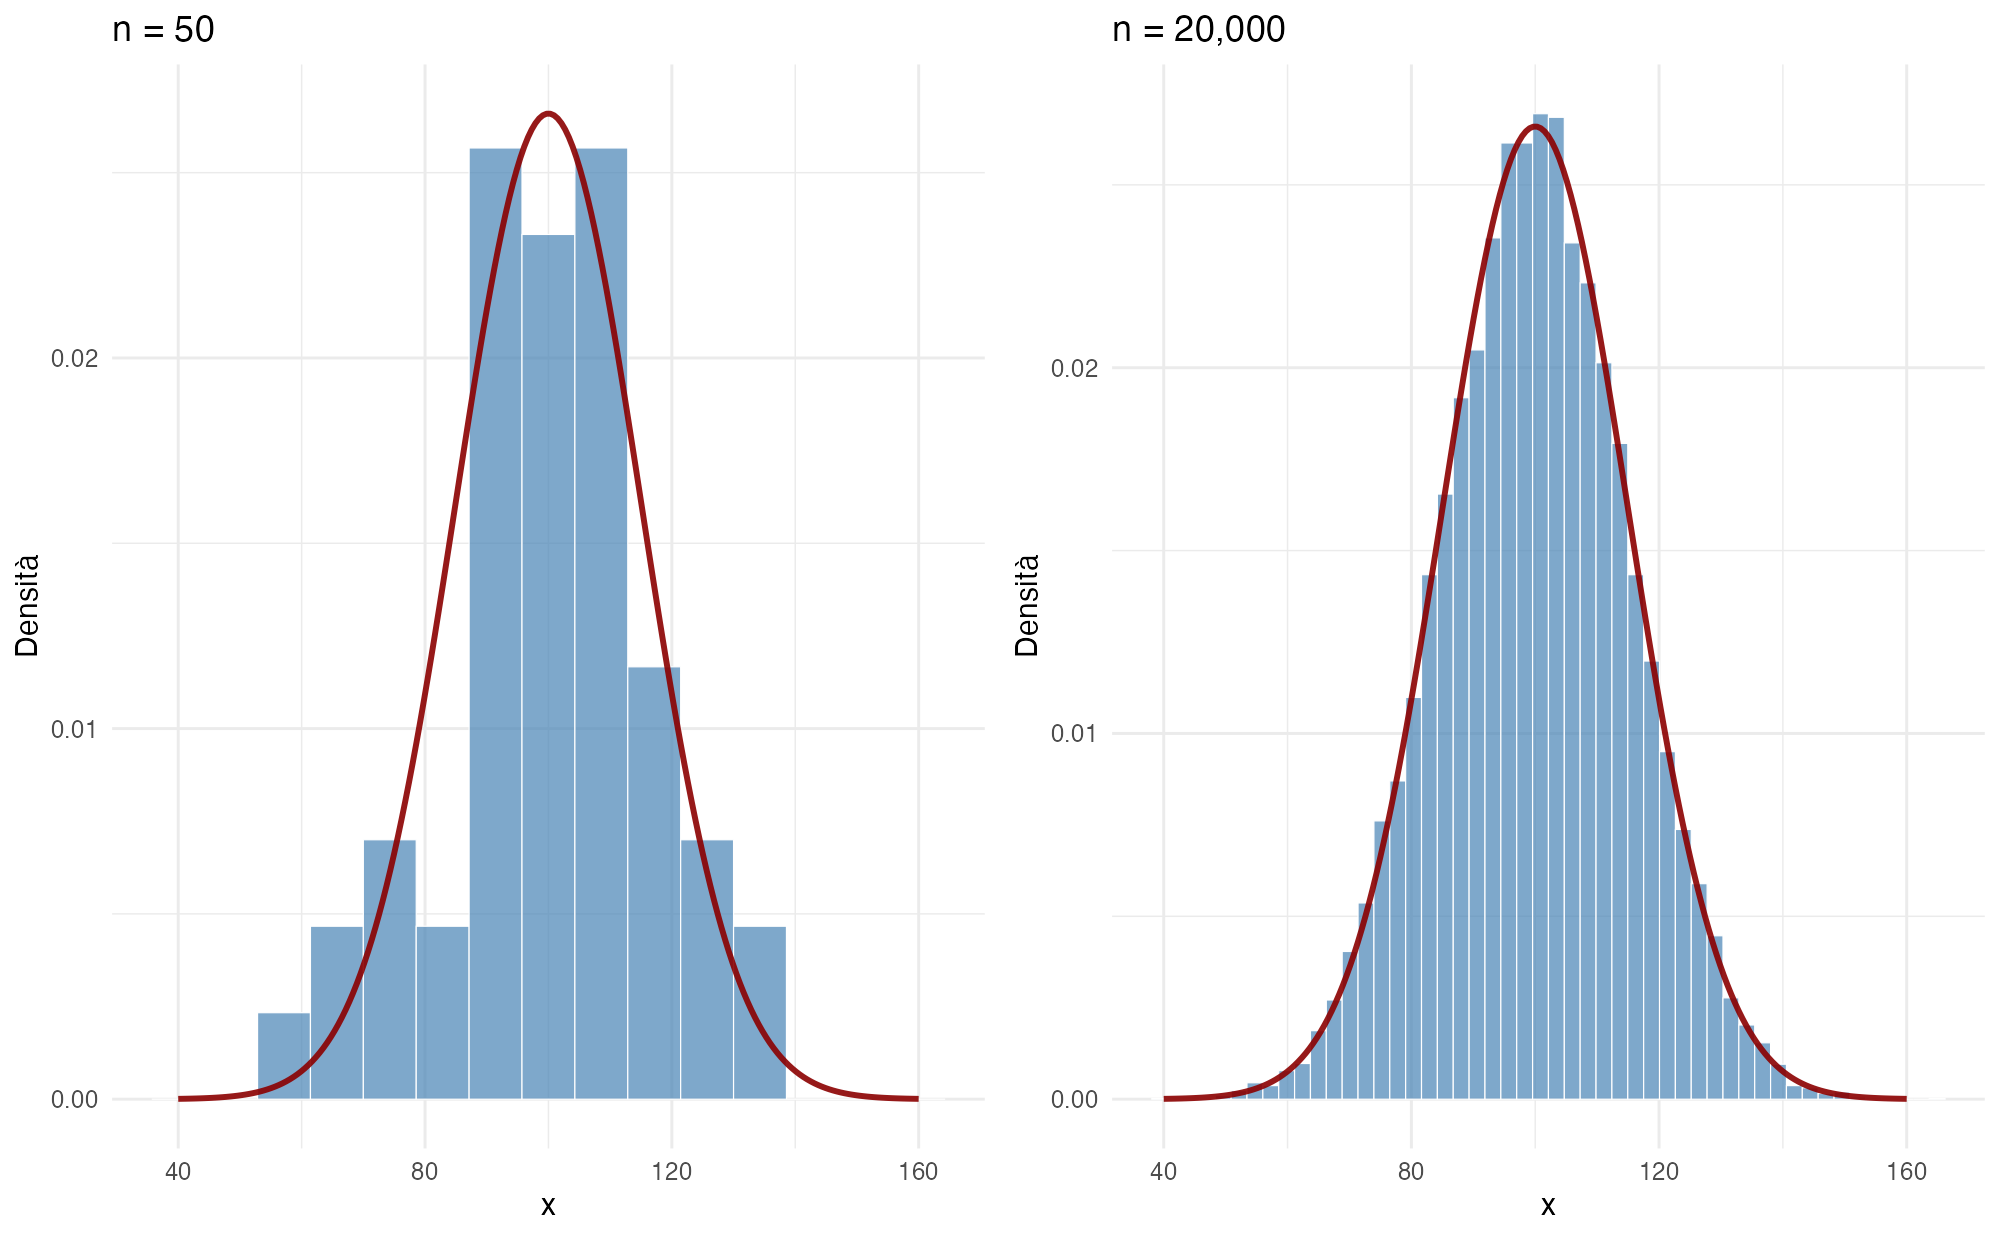
\includegraphics[width=0.85\linewidth,height=\textheight,keepaspectratio]{chapters/probability/07_prob_distributions_files/figure-pdf/fig-histogram-to-density-1.png}

}

\caption{\label{fig-histogram-to-density}Convergenza dell'istogramma
alla PDF teorica (distribuzione normale) all'aumentare della dimensione
campionaria. Con n = 50 (sinistra), l'approssimazione è grezza; con n =
20,000 (destra), l'istogramma aderisce strettamente alla curva teorica.}

\end{figure}%

La PDF, dunque, cattura l'essenza della variabilità di una popolazione,
non i dettagli di ogni singola osservazione, ma il pattern sottostante
che emerge quando si aggrega un gran numero di osservazioni. Si tratta
di un modello idealizzato che sacrifica la complessità del reale per
ottenere un maggiore potere predittivo e analitico.

\section{Il paradosso della probabilità
nulla}\label{il-paradosso-della-probabilituxe0-nulla}

Una delle proprietà più controintuitive delle variabili casuali continue
risiede nel fatto che la probabilità di osservare \emph{esattamente} un
qualsiasi valore specifico è identicamente nulla: \[
P(X = x_0) = 0 \quad \text{per ogni } x_0 \in \mathbb{R}.
\]

Questo risultato solleva un apparente paradosso epistemologico: se ogni
singolo valore ha probabilità nulla, come è possibile osservare
empiricamente un valore qualsiasi? In altre parole, quando misuriamo
un'altezza di 170 cm, non stiamo forse constatando il verificarsi di un
evento che la teoria considera avere una probabilità pari a zero?

\subsection{Fondamento matematico della probabilità puntuale
nulla}\label{fondamento-matematico-della-probabilituxe0-puntuale-nulla}

La spiegazione risiede nella natura stessa dell'integrazione. Per una
variabile continua, la probabilità associata a un singolo punto
corrisponde all'integrale della funzione di densità su un intervallo di
misura nulla: \[
P(X = x_0) = \int_{x_0}^{x_0} f_X(x)  dx = 0.
\]

L'area sottesa da qualsiasi curva, calcolata su un intervallo di
ampiezza infinitesima, è necessariamente zero. Ciò non rappresenta una
lacuna della teoria, ma una conseguenza intrinseca del continuo
matematico.

Un'ulteriore prospettiva chiarificatrice emerge considerando il vincolo
di normalizzazione. Se ogni punto in un intervallo {[}a, b{]} avesse una
probabilità positiva \(\epsilon > 0\), la ``somma'' delle probabilità
sull'insieme non numerabile dei punti reali condurrebbe a una
contraddizione con il principio di normalizzazione
\(\int_{-\infty}^{\infty} f_X(x) dx = 1\). L'unica configurazione
coerente con il principio di normalizzazione richiede che la probabilità
associata a ogni singolo punto sia esattamente zero.

\subsection{La prospettiva degli
infinitesimi}\label{la-prospettiva-degli-infinitesimi}

Un modo alternativo per affrontare l'apparente paradosso della
probabilità nulla nei modelli continui proviene dalla teoria dei numeri
iperreali, introdotta da Abraham Robinson negli anni '60. Senza entrare
nei dettagli tecnici, questa teoria permette di immaginare quantità
infinitesimali, ovvero numeri positivi così piccoli da essere inferiori
a qualsiasi numero reale, ma comunque diversi da zero.

L'idea intuitiva è la seguente:

\begin{itemize}
\tightlist
\item
  a un singolo punto (x\_0) si può associare una probabilità
  infinitesimale, non esattamente pari a zero, ma talmente piccola da
  poter essere trascurata in pratica;
\item
  una probabilità finita per un intervallo, come ({[}a,b{]}), è data
  dalla somma di un numero enorme di contributi infinitesimali, uno per
  ciascun punto dell'intervallo;
\item
  più la ``partizione'' dell'intervallo diventa fine, più questi
  contributi infinitesimali si avvicinano al concetto matematico di
  integrazione.
\end{itemize}

Questa prospettiva non modifica i risultati della teoria classica, ma
offre un modo intuitivo di pensare alla situazione: una singola misura
puntuale ha un peso ``quasi nullo'', mentre un insieme continuo di punti
accumula contributi sufficienti a generare una probabilità finita. Si
tratta di un modo elegante per conciliare l'intuizione con il rigore
della matematica moderna.

\begin{tcolorbox}[enhanced jigsaw, arc=.35mm, breakable, colbacktitle=quarto-callout-note-color!10!white, opacityback=0, toprule=.15mm, rightrule=.15mm, colback=white, opacitybacktitle=0.6, leftrule=.75mm, coltitle=black, bottomtitle=1mm, left=2mm, toptitle=1mm, title=\textcolor{quarto-callout-note-color}{\faInfo}\hspace{0.5em}{Esempio: Il paradosso di Zenone}, titlerule=0mm, bottomrule=.15mm, colframe=quarto-callout-note-color-frame]

\subsubsection*{Un'analogia classica}\label{unanalogia-classica}

Il paradosso della probabilità zero ricorda il celebre paradosso di
Zenone della freccia. Zenone sosteneva che, in ogni istante, la freccia
occupa una posizione fissa e quindi è ``immobile''; ma se è immobile in
ogni istante, come può muoversi?

La risoluzione moderna riconosce che il movimento non è la somma di
posizioni statiche, ma emerge dall'integrazione su un continuum di
istanti. Allo stesso modo, la probabilità di una variabile continua non
è la ``somma'' di probabilità puntuali (che sarebbero tutte pari a
zero), ma l'integrale della densità su intervalli.

In entrambi i casi, il paradosso nasce dall'applicazione di intuizioni
discrete a contesti continui. Il passaggio al continuo richiede
strumenti matematici come limiti, integrali e teoria della misura, che
vanno oltre l'aritmetica ordinaria.

\end{tcolorbox}

\subsection{Implicazioni pratiche}\label{implicazioni-pratiche}

Questa proprietà ha importanti conseguenze operative. Per le variabili
continue, non ha senso chiedersi: ``Qual è la probabilità che il tempo
di reazione sia esattamente 250 ms?''. La domanda corretta è: ``Qual è
la probabilità che il tempo di reazione sia compreso tra 245 e 255 ms?''
Le probabilità si calcolano sempre su \textbf{intervalli}, mai su punti
singoli.

Un corollario utile è che, per le variabili continue, includere o
escludere gli estremi di un intervallo non modifica la probabilità: \[
P(a < X < b) = P(a \leq X < b) = P(a < X \leq b) = P(a \leq X \leq b).
\]

Ciò è vero perché i singoli punti \(a\) e \(b\) hanno ciascuno
probabilità zero.

\section{La funzione di distribuzione
cumulativa}\label{la-funzione-di-distribuzione-cumulativa}

La funzione di distribuzione cumulativa (CDF) offre una rappresentazione
unificata delle distribuzioni di probabilità, valida sia per le
variabili discrete che per quelle continue. Per qualsiasi variabile
casuale \(X\), la CDF è definita come:

\begin{definition}[Funzione di distribuzione
cumulativa]\protect\hypertarget{def-cdf-unified}{}\label{def-cdf-unified}

La \emph{funzione di distribuzione cumulativa} di una variabile casuale
\(X\) è: \[
F_X(x) = P(X \leq x).
\]

\end{definition}

Questa definizione è universale e non dipende dal fatto che \(X\) sia
discreta o continua. La CDF ``accumula'' la probabilità da \(-\infty\)
fino al valore \(x\), fornendo una misura della probabilità che la
variabile assuma valori non superiori a \(x\).

\subsection{Proprietà fondamentali della
CDF}\label{proprietuxe0-fondamentali-della-cdf}

Ogni funzione di distribuzione cumulativa soddisfa tre proprietà che ne
caratterizzano completamente il comportamento.

\begin{theorem}[Proprietà della
CDF]\protect\hypertarget{thm-cdf-properties-detail}{}\label{thm-cdf-properties-detail}

Per qualsiasi variabile casuale \(X\), la CDF \(F_X\) soddisfa:

\begin{enumerate}
\def\labelenumi{\arabic{enumi}.}
\tightlist
\item
  \textbf{Monotonia non decrescente}: Se \(a < b\), allora
  \(F_X(a) \leq F_X(b)\).
\item
  \textbf{Limiti agli estremi}: \(\lim_{x \to -\infty} F_X(x) = 0\) e
  \(\lim_{x \to +\infty} F_X(x) = 1\).
\item
  \textbf{Continuità a destra}: \(\lim_{h \to 0^+} F_X(x + h) = F_X(x)\)
  per ogni \(x\).
\end{enumerate}

\end{theorem}

La monotonia riflette il fatto che, estendendo l'intervallo
\((-\infty, x]\), non è possibile perdere probabilità. I limiti
garantiscono la normalizzazione: nessuna probabilità per i valori
infinitamente piccoli e tutta la probabilità per i valori infinitamente
grandi. La continuità a destra è una convenzione tecnica che risolve le
ambiguità nei punti di discontinuità, presenti solo per le variabili
discrete.

\subsection{CDF per variabili discrete e
continue}\label{cdf-per-variabili-discrete-e-continue}

Per le variabili \emph{discrete}, la CDF è una funzione a gradini:
rimane costante tra i valori possibili e presenta un salto in
corrispondenza di ogni valore con massa positiva. L'altezza del salto in
\(x_i\) è esattamente \(p_X(x_i)\).

Per le variabili \emph{continue}, la CDF è una funzione continua e
tipicamente differenziabile. La derivata della CDF restituisce la PDF:
\[
f_X(x) = \frac{d}{dx} F_X(x).
\]

Reciprocamente, la CDF si ottiene integrando la PDF: \[
F_X(x) = \int_{-\infty}^{x} f_X(t) \, dt.
\]

\begin{Shaded}
\begin{Highlighting}[]
\CommentTok{\# CDF discreta (dado equilibrato)}
\NormalTok{x\_disc }\OtherTok{\textless{}{-}} \DecValTok{0}\SpecialCharTok{:}\DecValTok{7}
\NormalTok{cdf\_disc }\OtherTok{\textless{}{-}} \FunctionTok{c}\NormalTok{(}\DecValTok{0}\NormalTok{, }\FunctionTok{cumsum}\NormalTok{(}\FunctionTok{rep}\NormalTok{(}\DecValTok{1}\SpecialCharTok{/}\DecValTok{6}\NormalTok{, }\DecValTok{6}\NormalTok{)), }\DecValTok{1}\NormalTok{)}

\NormalTok{df\_disc }\OtherTok{\textless{}{-}} \FunctionTok{data.frame}\NormalTok{(}\AttributeTok{x\_start =}\NormalTok{ x\_disc[}\SpecialCharTok{{-}}\FunctionTok{length}\NormalTok{(x\_disc)], }
                      \AttributeTok{x\_end =}\NormalTok{ x\_disc[}\SpecialCharTok{{-}}\DecValTok{1}\NormalTok{], }
                      \AttributeTok{y =}\NormalTok{ cdf\_disc[}\SpecialCharTok{{-}}\FunctionTok{length}\NormalTok{(cdf\_disc)])}

\NormalTok{p1 }\OtherTok{\textless{}{-}} \FunctionTok{ggplot}\NormalTok{() }\SpecialCharTok{+}
  \FunctionTok{geom\_segment}\NormalTok{(}\AttributeTok{data =}\NormalTok{ df\_disc, }\FunctionTok{aes}\NormalTok{(}\AttributeTok{x =}\NormalTok{ x\_start, }\AttributeTok{xend =}\NormalTok{ x\_end, }\AttributeTok{y =}\NormalTok{ y, }\AttributeTok{yend =}\NormalTok{ y),}
               \AttributeTok{linewidth =} \DecValTok{1}\NormalTok{, }\AttributeTok{color =} \StringTok{"steelblue"}\NormalTok{) }\SpecialCharTok{+}
  \FunctionTok{geom\_point}\NormalTok{(}\AttributeTok{data =} \FunctionTok{data.frame}\NormalTok{(}\AttributeTok{x =} \DecValTok{1}\SpecialCharTok{:}\DecValTok{6}\NormalTok{, }\AttributeTok{y =} \FunctionTok{cumsum}\NormalTok{(}\FunctionTok{rep}\NormalTok{(}\DecValTok{1}\SpecialCharTok{/}\DecValTok{6}\NormalTok{, }\DecValTok{6}\NormalTok{))),}
             \FunctionTok{aes}\NormalTok{(}\AttributeTok{x =}\NormalTok{ x, }\AttributeTok{y =}\NormalTok{ y), }\AttributeTok{size =} \DecValTok{3}\NormalTok{, }\AttributeTok{color =} \StringTok{"steelblue"}\NormalTok{) }\SpecialCharTok{+}
  \FunctionTok{geom\_point}\NormalTok{(}\AttributeTok{data =} \FunctionTok{data.frame}\NormalTok{(}\AttributeTok{x =} \DecValTok{1}\SpecialCharTok{:}\DecValTok{6}\NormalTok{, }\AttributeTok{y =} \FunctionTok{c}\NormalTok{(}\DecValTok{0}\NormalTok{, }\FunctionTok{cumsum}\NormalTok{(}\FunctionTok{rep}\NormalTok{(}\DecValTok{1}\SpecialCharTok{/}\DecValTok{6}\NormalTok{, }\DecValTok{5}\NormalTok{)))),}
             \FunctionTok{aes}\NormalTok{(}\AttributeTok{x =}\NormalTok{ x, }\AttributeTok{y =}\NormalTok{ y), }\AttributeTok{size =} \DecValTok{3}\NormalTok{, }\AttributeTok{color =} \StringTok{"steelblue"}\NormalTok{, }\AttributeTok{shape =} \DecValTok{1}\NormalTok{) }\SpecialCharTok{+}
  \FunctionTok{scale\_x\_continuous}\NormalTok{(}\AttributeTok{breaks =} \DecValTok{0}\SpecialCharTok{:}\DecValTok{7}\NormalTok{, }\AttributeTok{limits =} \FunctionTok{c}\NormalTok{(}\DecValTok{0}\NormalTok{, }\DecValTok{7}\NormalTok{)) }\SpecialCharTok{+}
  \FunctionTok{scale\_y\_continuous}\NormalTok{(}\AttributeTok{breaks =} \FunctionTok{seq}\NormalTok{(}\DecValTok{0}\NormalTok{, }\DecValTok{1}\NormalTok{, }\FloatTok{0.2}\NormalTok{)) }\SpecialCharTok{+}
  \FunctionTok{labs}\NormalTok{(}\AttributeTok{title =} \StringTok{"CDF discreta (dado equilibrato)"}\NormalTok{, }
       \AttributeTok{x =} \StringTok{"x"}\NormalTok{, }\AttributeTok{y =} \FunctionTok{expression}\NormalTok{(F[X](x))) }\SpecialCharTok{+}
  \FunctionTok{theme\_minimal}\NormalTok{()}

\CommentTok{\# CDF continua (normale standard)}
\NormalTok{x\_cont }\OtherTok{\textless{}{-}} \FunctionTok{seq}\NormalTok{(}\SpecialCharTok{{-}}\DecValTok{4}\NormalTok{, }\DecValTok{4}\NormalTok{, }\AttributeTok{length.out =} \DecValTok{200}\NormalTok{)}
\NormalTok{cdf\_cont }\OtherTok{\textless{}{-}} \FunctionTok{pnorm}\NormalTok{(x\_cont)}

\NormalTok{p2 }\OtherTok{\textless{}{-}} \FunctionTok{ggplot}\NormalTok{(}\FunctionTok{data.frame}\NormalTok{(}\AttributeTok{x =}\NormalTok{ x\_cont, }\AttributeTok{y =}\NormalTok{ cdf\_cont), }\FunctionTok{aes}\NormalTok{(}\AttributeTok{x =}\NormalTok{ x, }\AttributeTok{y =}\NormalTok{ y)) }\SpecialCharTok{+}
  \FunctionTok{geom\_line}\NormalTok{(}\AttributeTok{linewidth =} \DecValTok{1}\NormalTok{, }\AttributeTok{color =} \StringTok{"steelblue"}\NormalTok{) }\SpecialCharTok{+}
  \FunctionTok{scale\_y\_continuous}\NormalTok{(}\AttributeTok{breaks =} \FunctionTok{seq}\NormalTok{(}\DecValTok{0}\NormalTok{, }\DecValTok{1}\NormalTok{, }\FloatTok{0.2}\NormalTok{)) }\SpecialCharTok{+}
  \FunctionTok{labs}\NormalTok{(}\AttributeTok{title =} \StringTok{"CDF continua (normale standard)"}\NormalTok{, }
       \AttributeTok{x =} \StringTok{"x"}\NormalTok{, }\AttributeTok{y =} \FunctionTok{expression}\NormalTok{(F[X](x))) }\SpecialCharTok{+}
  \FunctionTok{theme\_minimal}\NormalTok{()}

\NormalTok{gridExtra}\SpecialCharTok{::}\FunctionTok{grid.arrange}\NormalTok{(p1, p2, }\AttributeTok{ncol =} \DecValTok{2}\NormalTok{)}
\end{Highlighting}
\end{Shaded}

\begin{figure}[H]

\centering{

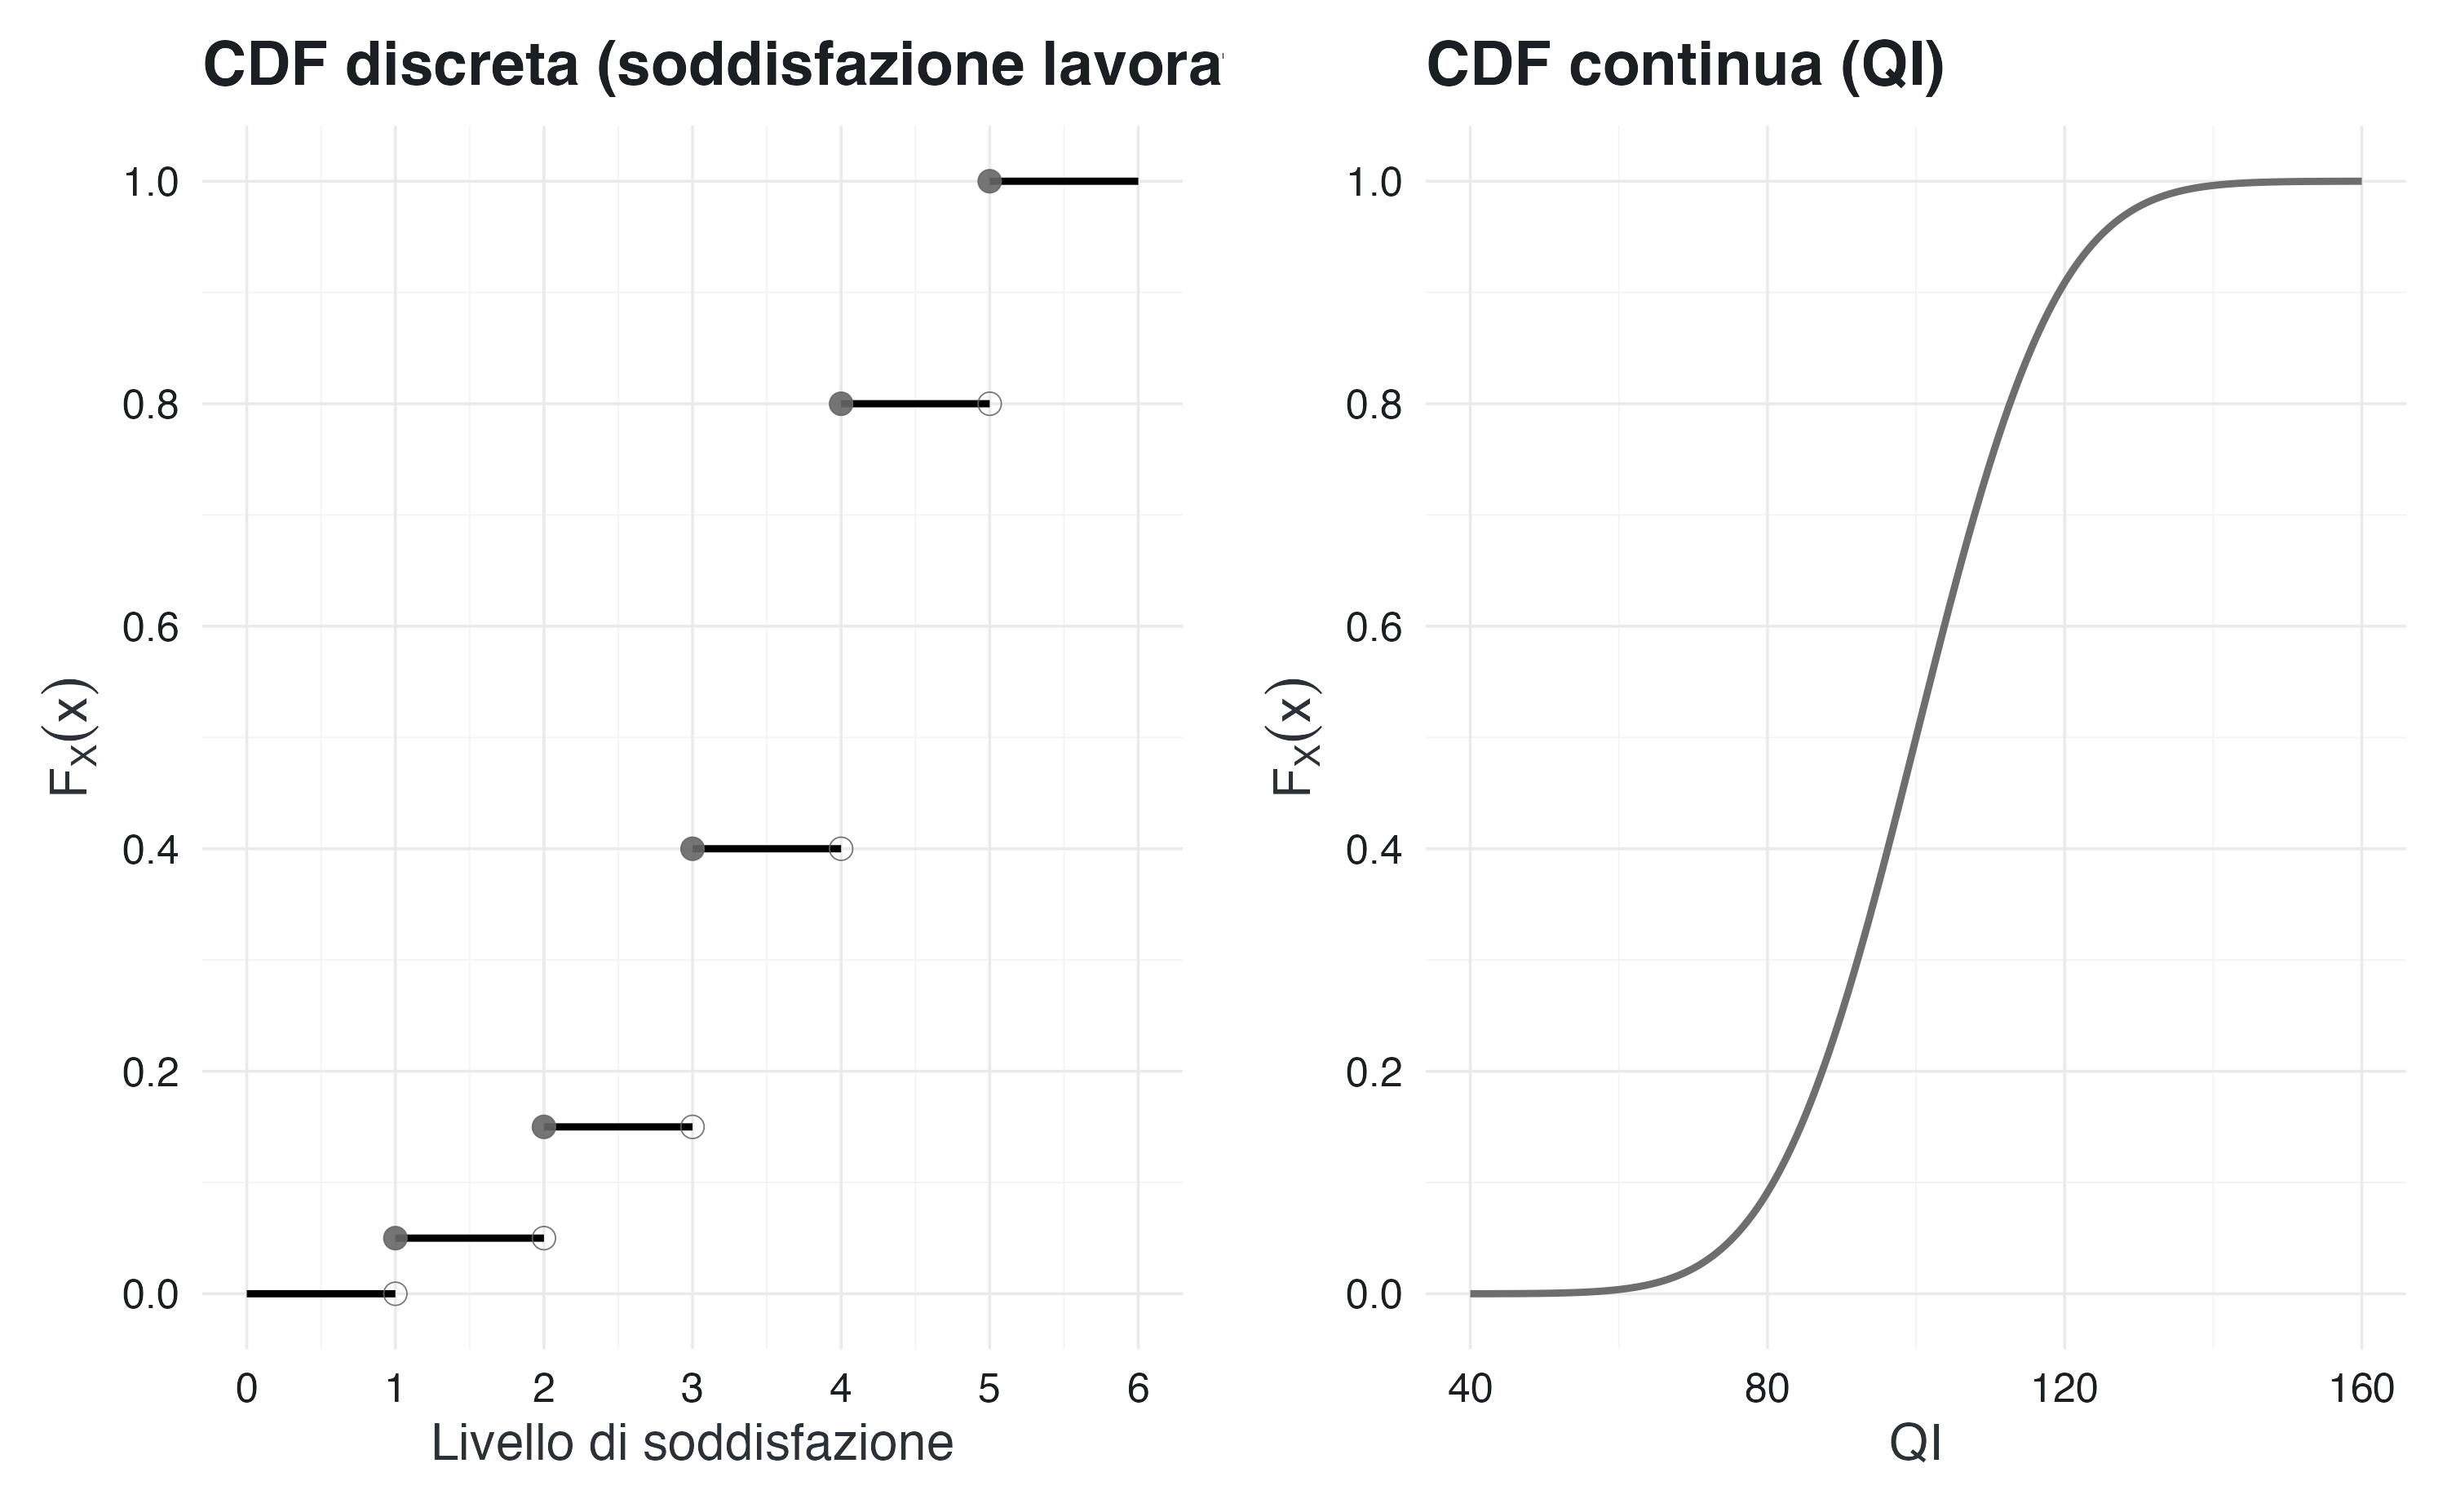
\includegraphics[width=0.85\linewidth,height=\textheight,keepaspectratio]{chapters/probability/07_prob_distributions_files/figure-pdf/fig-cdf-comparison-1.png}

}

\caption{\label{fig-cdf-comparison}CDF di una variabile discreta
(sinistra, a gradini) e di una variabile continua (destra, curva
liscia). Per la variabile discreta, i salti corrispondono ai valori con
massa positiva; per la variabile continua, la CDF è derivabile ovunque.}

\end{figure}%

\subsection{Calcolo di probabilità mediante la
CDF}\label{calcolo-di-probabilituxe0-mediante-la-cdf}

La CDF permette di calcolare la probabilità di qualsiasi intervallo
attraverso una semplice differenza: \[
P(a < X \leq b) = F_X(b) - F_X(a).
\]

Questa formula è valida sia per le variabili discrete che per quelle
continue e rappresenta uno degli strumenti computazionali più utili
nella pratica statistica.

\begin{tcolorbox}[enhanced jigsaw, arc=.35mm, breakable, colbacktitle=quarto-callout-note-color!10!white, opacityback=0, toprule=.15mm, rightrule=.15mm, colback=white, opacitybacktitle=0.6, leftrule=.75mm, coltitle=black, bottomtitle=1mm, left=2mm, toptitle=1mm, title=\textcolor{quarto-callout-note-color}{\faInfo}\hspace{0.5em}{Esempio: Calcoli con la CDF normale}, titlerule=0mm, bottomrule=.15mm, colframe=quarto-callout-note-color-frame]

\subsubsection*{Probabilità per la distribuzione
normale}\label{probabilituxe0-per-la-distribuzione-normale}

Consideriamo il quoziente intellettivo (QI), modellato come variabile
normale con media \(\mu = 100\) e deviazione standard \(\sigma = 15\).
Calcoliamo alcune probabilità di interesse clinico.

\begin{Shaded}
\begin{Highlighting}[]
\NormalTok{mu }\OtherTok{\textless{}{-}} \DecValTok{100}
\NormalTok{sigma }\OtherTok{\textless{}{-}} \DecValTok{15}

\CommentTok{\# P(QI \textgreater{} 130) {-} QI molto elevato}
\NormalTok{p\_alto }\OtherTok{\textless{}{-}} \DecValTok{1} \SpecialCharTok{{-}} \FunctionTok{pnorm}\NormalTok{(}\DecValTok{130}\NormalTok{, }\AttributeTok{mean =}\NormalTok{ mu, }\AttributeTok{sd =}\NormalTok{ sigma)}
\FunctionTok{cat}\NormalTok{(}\StringTok{"P(QI \textgreater{} 130) ="}\NormalTok{, }\FunctionTok{round}\NormalTok{(p\_alto, }\DecValTok{4}\NormalTok{), }\StringTok{"}\SpecialCharTok{\textbackslash{}n}\StringTok{"}\NormalTok{)}
\CommentTok{\#\textgreater{} P(QI \textgreater{} 130) = 0.0228}

\CommentTok{\# P(85 \textless{} QI \textless{} 115) {-} QI nella norma (±1 SD)}
\NormalTok{p\_norma }\OtherTok{\textless{}{-}} \FunctionTok{pnorm}\NormalTok{(}\DecValTok{115}\NormalTok{, }\AttributeTok{mean =}\NormalTok{ mu, }\AttributeTok{sd =}\NormalTok{ sigma) }\SpecialCharTok{{-}} \FunctionTok{pnorm}\NormalTok{(}\DecValTok{85}\NormalTok{, }\AttributeTok{mean =}\NormalTok{ mu, }\AttributeTok{sd =}\NormalTok{ sigma)}
\FunctionTok{cat}\NormalTok{(}\StringTok{"P(85 \textless{} QI \textless{} 115) ="}\NormalTok{, }\FunctionTok{round}\NormalTok{(p\_norma, }\DecValTok{4}\NormalTok{), }\StringTok{"}\SpecialCharTok{\textbackslash{}n}\StringTok{"}\NormalTok{)}
\CommentTok{\#\textgreater{} P(85 \textless{} QI \textless{} 115) = 0.683}

\CommentTok{\# P(QI \textless{} 70) {-} disabilità intellettiva}
\NormalTok{p\_basso }\OtherTok{\textless{}{-}} \FunctionTok{pnorm}\NormalTok{(}\DecValTok{70}\NormalTok{, }\AttributeTok{mean =}\NormalTok{ mu, }\AttributeTok{sd =}\NormalTok{ sigma)}
\FunctionTok{cat}\NormalTok{(}\StringTok{"P(QI \textless{} 70) ="}\NormalTok{, }\FunctionTok{round}\NormalTok{(p\_basso, }\DecValTok{4}\NormalTok{), }\StringTok{"}\SpecialCharTok{\textbackslash{}n}\StringTok{"}\NormalTok{)}
\CommentTok{\#\textgreater{} P(QI \textless{} 70) = 0.0228}

\CommentTok{\# Percentile 95}
\NormalTok{q95 }\OtherTok{\textless{}{-}} \FunctionTok{qnorm}\NormalTok{(}\FloatTok{0.95}\NormalTok{, }\AttributeTok{mean =}\NormalTok{ mu, }\AttributeTok{sd =}\NormalTok{ sigma)}
\FunctionTok{cat}\NormalTok{(}\StringTok{"95° percentile:"}\NormalTok{, }\FunctionTok{round}\NormalTok{(q95, }\DecValTok{1}\NormalTok{), }\StringTok{"}\SpecialCharTok{\textbackslash{}n}\StringTok{"}\NormalTok{)}
\CommentTok{\#\textgreater{} 95° percentile: 125}
\end{Highlighting}
\end{Shaded}

Questi calcoli illustrano come la CDF (implementata in R dalla funzione
\texttt{pnorm}) permetta di tradurre domande cliniche in operazioni
matematiche precise.

\end{tcolorbox}

\section{Interpretazioni bayesiana e
frequentista}\label{interpretazioni-bayesiana-e-frequentista}

Le distribuzioni di probabilità assumono significati profondamente
diversi nei due principali paradigmi dell'inferenza statistica. Questa
distinzione, apparentemente filosofica, ha conseguenze concrete per
l'interpretazione dei risultati e la costruzione dei modelli.

\subsection{L'interpretazione
frequentista}\label{linterpretazione-frequentista}

Nel paradigma frequentista, la PDF descrive la distribuzione dei dati in
una serie ipotetica di ripetizioni dell'esperimento. La probabilità è
definita come il limite della frequenza relativa: \[
P(a \leq X \leq b) = \lim_{n \to \infty} \frac{\#\{X_i \in [a, b]\}}{n}
\] dove \(X_1, X_2, \ldots\) sono osservazioni indipendenti generate
dallo stesso processo.

In questa prospettiva, la PDF è l'\emph{istogramma limite}: il profilo
che emerge quando aggreghiamo un numero infinito di osservazioni in
intervalli infinitamente piccoli. La variabile \(X\) rappresenta il
risultato di un esperimento ripetibile, e la PDF descrive la variabilità
\emph{tra} le ripetizioni.

Un esempio paradigmatico è la misurazione dell'altezza in una
popolazione. La PDF normale con \(\mu = 170\) cm e \(\sigma = 10\) cm
descrive quale frazione di individui troveremmo in ogni intervallo di
altezza se potessimo misurare l'intera popolazione infinita.

\subsection{L'interpretazione
bayesiana}\label{linterpretazione-bayesiana}

Nel paradigma bayesiano, la PDF quantifica il nostro \emph{grado di
credenza} sui possibili valori di una quantità incerta. La probabilità
non richiede ripetizioni ipotetiche: è una proprietà del nostro stato di
conoscenza, non del mondo esterno.

\begin{definition}[Interpretazione bayesiana della
PDF]\protect\hypertarget{def-bayesian-pdf}{}\label{def-bayesian-pdf}

In una prospettiva bayesiana, la funzione di densità \(f_X(x)\)
rappresenta la \emph{distribuzione della credenza} su una quantità \(X\)
il cui valore vero è fisso ma sconosciuto. L'integrale
\(\int_a^b f_X(x) dx\) quantifica quanto fortemente crediamo che il
valore vero cada nell'intervallo \([a, b]\).

\end{definition}

La differenza cruciale è che nell'approccio bayesiano non è necessario
immaginare la ripetizione dell'esperimento. È possibile assegnare
distribuzioni di probabilità a parametri fissi (come l'effetto medio di
un trattamento sulla popolazione) o a eventi unici (come la probabilità
che un determinato paziente risponda alla terapia).

La PDF bayesiana può essere meglio visualizzata come una ``mappa di
plausibilità'': le regioni con una densità alta corrispondono a valori
che consideriamo più credibili, mentre le regioni con una densità bassa
corrispondono a valori meno plausibili. La forma della distribuzione,
con le sue code, la sua simmetria o asimmetria, la sua concentrazione o
dispersione, codifica tutto ciò che sappiamo (e non sappiamo) sulla
quantità di interesse.

\subsection{Confronto tra le due
prospettive}\label{confronto-tra-le-due-prospettive}

Le differenze tra i due approcci emergono chiaramente in un esempio
concreto. Supponiamo di voler stimare l'altezza media \(\theta\) di una
popolazione.

Nel paradigma frequentista, \(\theta\) è un parametro fisso, ma
sconosciuto. La PDF della media campionaria \(\bar{X}\) (non di
\(\theta\)!) descrive come \(\bar{X}\) varierebbe in campioni ripetuti
dalla stessa popolazione. Un intervallo di confidenza al 95\% non
significa che l'altezza media ha il 95\% di probabilità di trovarsi
nell'intervallo, dato che l'altezza media è un valore fisso e non
casuale, ma che la procedura che genera l'intervallo ``cattura'' il
valore vero dell'altezza media nel 95\% delle ripetizioni.

Nel paradigma bayesiano, invece, si assegna direttamente una
distribuzione di probabilità a \(\theta\). Questa distribuzione a priori
rappresenta le nostre credenze prima di osservare i dati, mentre la
distribuzione a posteriori le aggiorna alla luce delle osservazioni. Un
intervallo di credibilità al 95\% significa esattamente ciò che sembra:
crediamo con probabilità 0,95 che il valore di \(\theta\) si trovi
nell'intervallo.

\begin{Shaded}
\begin{Highlighting}[]
\FunctionTok{set.seed}\NormalTok{(}\DecValTok{123}\NormalTok{)}

\CommentTok{\# Frequentista: distribuzione dei dati}
\NormalTok{x\_freq }\OtherTok{\textless{}{-}} \FunctionTok{rnorm}\NormalTok{(}\DecValTok{1000}\NormalTok{, }\AttributeTok{mean =} \DecValTok{170}\NormalTok{, }\AttributeTok{sd =} \DecValTok{10}\NormalTok{)}
\NormalTok{x\_seq }\OtherTok{\textless{}{-}} \FunctionTok{seq}\NormalTok{(}\DecValTok{140}\NormalTok{, }\DecValTok{200}\NormalTok{, }\AttributeTok{length.out =} \DecValTok{200}\NormalTok{)}
\NormalTok{y\_teorica }\OtherTok{\textless{}{-}} \FunctionTok{dnorm}\NormalTok{(x\_seq, }\AttributeTok{mean =} \DecValTok{170}\NormalTok{, }\AttributeTok{sd =} \DecValTok{10}\NormalTok{)}

\NormalTok{p1 }\OtherTok{\textless{}{-}} \FunctionTok{ggplot}\NormalTok{() }\SpecialCharTok{+}
  \FunctionTok{geom\_histogram}\NormalTok{(}\AttributeTok{data =} \FunctionTok{data.frame}\NormalTok{(}\AttributeTok{x =}\NormalTok{ x\_freq), }\FunctionTok{aes}\NormalTok{(}\AttributeTok{x =}\NormalTok{ x, }\AttributeTok{y =} \FunctionTok{after\_stat}\NormalTok{(density)),}
                 \AttributeTok{bins =} \DecValTok{30}\NormalTok{, }\AttributeTok{fill =} \StringTok{"steelblue"}\NormalTok{, }\AttributeTok{alpha =} \FloatTok{0.5}\NormalTok{, }\AttributeTok{color =} \StringTok{"white"}\NormalTok{) }\SpecialCharTok{+}
  \FunctionTok{geom\_line}\NormalTok{(}\AttributeTok{data =} \FunctionTok{data.frame}\NormalTok{(}\AttributeTok{x =}\NormalTok{ x\_seq, }\AttributeTok{y =}\NormalTok{ y\_teorica), }
            \FunctionTok{aes}\NormalTok{(}\AttributeTok{x =}\NormalTok{ x, }\AttributeTok{y =}\NormalTok{ y), }\AttributeTok{color =} \StringTok{"darkred"}\NormalTok{, }\AttributeTok{linewidth =} \FloatTok{1.2}\NormalTok{) }\SpecialCharTok{+}
  \FunctionTok{labs}\NormalTok{(}\AttributeTok{title =} \StringTok{"Frequentista: distribuzione dei dati"}\NormalTok{,}
       \AttributeTok{subtitle =} \StringTok{"PDF come istogramma limite di ripetizioni"}\NormalTok{,}
       \AttributeTok{x =} \StringTok{"Altezza (cm)"}\NormalTok{, }\AttributeTok{y =} \StringTok{"Densità"}\NormalTok{) }\SpecialCharTok{+}
  \FunctionTok{theme\_minimal}\NormalTok{()}

\CommentTok{\# Bayesiano: distribuzione della credenza su un parametro}
\NormalTok{theta\_seq }\OtherTok{\textless{}{-}} \FunctionTok{seq}\NormalTok{(}\DecValTok{165}\NormalTok{, }\DecValTok{175}\NormalTok{, }\AttributeTok{length.out =} \DecValTok{200}\NormalTok{)}
\NormalTok{prior }\OtherTok{\textless{}{-}} \FunctionTok{dnorm}\NormalTok{(theta\_seq, }\AttributeTok{mean =} \DecValTok{170}\NormalTok{, }\AttributeTok{sd =} \DecValTok{2}\NormalTok{)}

\NormalTok{p2 }\OtherTok{\textless{}{-}} \FunctionTok{ggplot}\NormalTok{() }\SpecialCharTok{+}
  \FunctionTok{geom\_ribbon}\NormalTok{(}\AttributeTok{data =} \FunctionTok{data.frame}\NormalTok{(}\AttributeTok{x =}\NormalTok{ theta\_seq, }\AttributeTok{y =}\NormalTok{ prior),}
              \FunctionTok{aes}\NormalTok{(}\AttributeTok{x =}\NormalTok{ x, }\AttributeTok{ymin =} \DecValTok{0}\NormalTok{, }\AttributeTok{ymax =}\NormalTok{ y), }
              \AttributeTok{fill =} \StringTok{"steelblue"}\NormalTok{, }\AttributeTok{alpha =} \FloatTok{0.3}\NormalTok{) }\SpecialCharTok{+}
  \FunctionTok{geom\_line}\NormalTok{(}\AttributeTok{data =} \FunctionTok{data.frame}\NormalTok{(}\AttributeTok{x =}\NormalTok{ theta\_seq, }\AttributeTok{y =}\NormalTok{ prior),}
            \FunctionTok{aes}\NormalTok{(}\AttributeTok{x =}\NormalTok{ x, }\AttributeTok{y =}\NormalTok{ y), }\AttributeTok{color =} \StringTok{"darkred"}\NormalTok{, }\AttributeTok{linewidth =} \FloatTok{1.2}\NormalTok{) }\SpecialCharTok{+}
  \FunctionTok{geom\_point}\NormalTok{(}\FunctionTok{aes}\NormalTok{(}\AttributeTok{x =} \DecValTok{170}\NormalTok{, }\AttributeTok{y =} \DecValTok{0}\NormalTok{), }\AttributeTok{size =} \DecValTok{3}\NormalTok{, }\AttributeTok{color =} \StringTok{"black"}\NormalTok{) }\SpecialCharTok{+}
  \FunctionTok{annotate}\NormalTok{(}\StringTok{"text"}\NormalTok{, }\AttributeTok{x =} \DecValTok{170}\NormalTok{, }\AttributeTok{y =} \SpecialCharTok{{-}}\FloatTok{0.02}\NormalTok{, }\AttributeTok{label =} \StringTok{"θ (valore vero ignoto)"}\NormalTok{, }\AttributeTok{size =} \DecValTok{3}\NormalTok{) }\SpecialCharTok{+}
  \FunctionTok{labs}\NormalTok{(}\AttributeTok{title =} \StringTok{"Bayesiano: distribuzione della credenza"}\NormalTok{,}
       \AttributeTok{subtitle =} \StringTok{"PDF come mappa di plausibilità sul parametro"}\NormalTok{,}
       \AttributeTok{x =} \FunctionTok{expression}\NormalTok{(theta }\SpecialCharTok{\textasciitilde{}} \StringTok{"(altezza media)"}\NormalTok{), }\AttributeTok{y =} \StringTok{"Densità"}\NormalTok{) }\SpecialCharTok{+}
  \FunctionTok{theme\_minimal}\NormalTok{()}

\NormalTok{gridExtra}\SpecialCharTok{::}\FunctionTok{grid.arrange}\NormalTok{(p1, p2, }\AttributeTok{ncol =} \DecValTok{2}\NormalTok{)}
\end{Highlighting}
\end{Shaded}

\begin{figure}[H]

\centering{

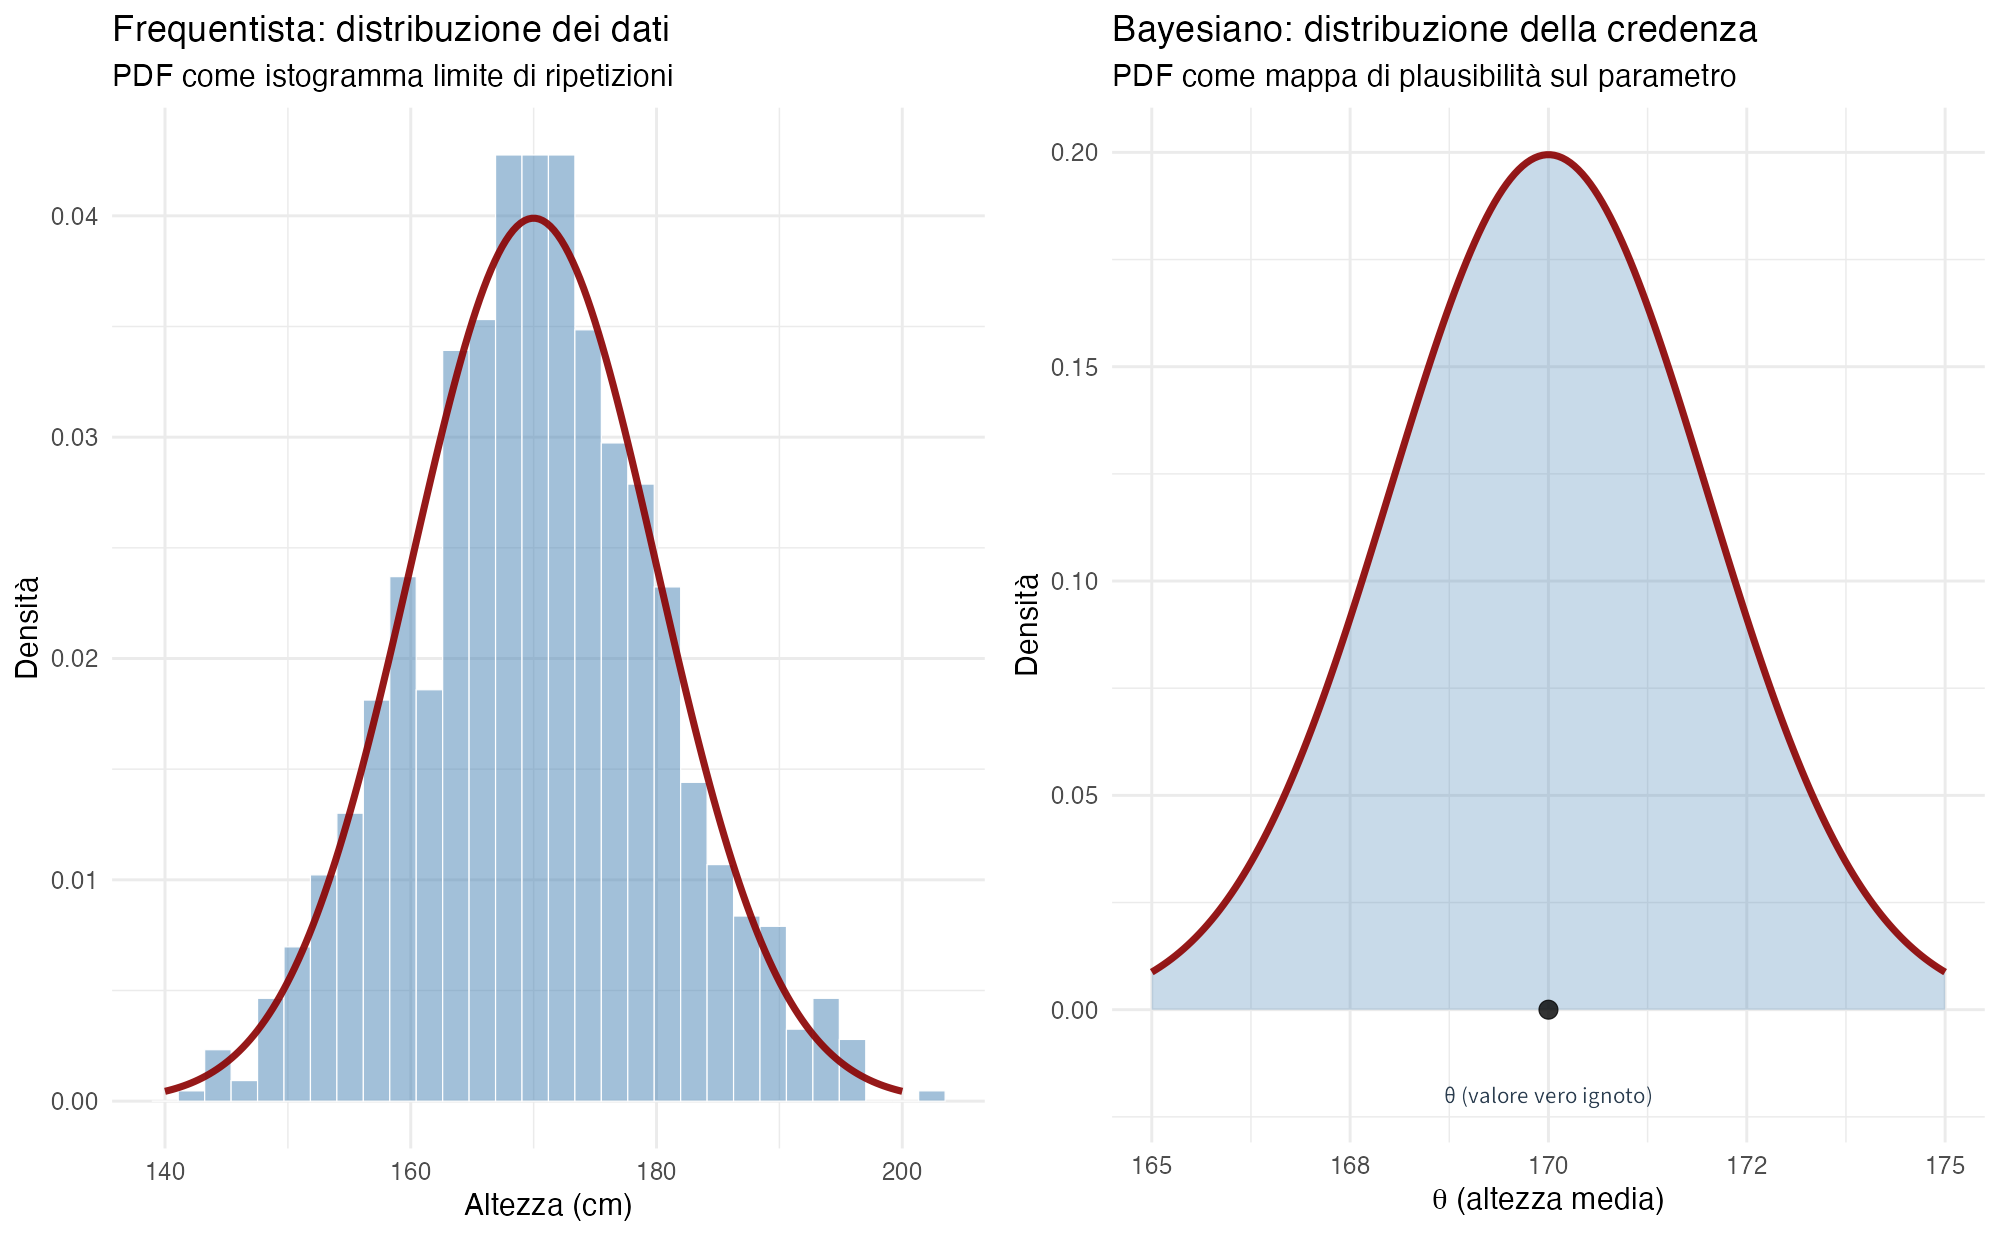
\includegraphics[width=0.85\linewidth,height=\textheight,keepaspectratio]{chapters/probability/07_prob_distributions_files/figure-pdf/fig-freq-vs-bayes-1.png}

}

\caption{\label{fig-freq-vs-bayes}Confronto tra interpretazioni
frequentista e bayesiana. A sinistra: la PDF descrive la distribuzione
dei dati (istogramma) in ripetizioni dell'esperimento. A destra: la PDF
rappresenta la credenza sul valore di un parametro, con l'incertezza
`spalmata' sui valori possibili.}

\end{figure}%

\section*{Riflessioni conclusive}\label{riflessioni-conclusive-6}

\markright{Riflessioni conclusive}

La distinzione concettuale tra massa e densità di probabilità riflette
una differenza fondamentale nella struttura matematica delle variabili
casuali discrete e continue. Per le variabili discrete, la probabilità
si manifesta come una grandezza ``concentrata'' in punti isolati dello
spazio campionario, mentre per le variabili continue è ``distribuita''
in modo continuo e può essere misurata esclusivamente mediante
l'integrazione su intervalli.

Il cosiddetto ``paradosso'' della probabilità nulla associata ai valori
esatti nelle distribuzioni continue si risolve non appena si riconosce
che, in questo contesto, la probabilità è intrinsecamente una proprietà
degli intervalli e non dei punti. Ogni singolo valore contribuisce con
una misura probabilistica nulla, eppure l'aggregazione di questa
infinità di contributi nulli, mediante il processo di integrazione,
produce probabilità finite e semanticamente significative.

La funzione di ripartizione (CDF) si presenta come uno strumento
unificante per le due classi di variabili, offrendo una rappresentazione
coerente in entrambi i contesti e consentendo il calcolo sistematico
delle probabilità per intervalli arbitrari.

Infine, la distinzione tra le interpretazioni frequentista e bayesiana
della probabilità non è una mera questione filosofica, ma ha
implicazioni operative concrete per la costruzione e l'interpretazione
dei modelli statistici. Poiché il nostro obiettivo è l'inferenza in
condizioni di incertezza, il corso si baserà sul paradigma bayesiano, il
cui apparato formale è specificamente progettato per aggiornare in modo
logicamente coerente lo stato della conoscenza alla luce dell'evidenza
empirica.

\begin{tcolorbox}[enhanced jigsaw, arc=.35mm, breakable, colbacktitle=quarto-callout-important-color!10!white, opacityback=0, toprule=.15mm, rightrule=.15mm, colback=white, opacitybacktitle=0.6, leftrule=.75mm, coltitle=black, bottomtitle=1mm, left=2mm, toptitle=1mm, title=\textcolor{quarto-callout-important-color}{\faExclamation}\hspace{0.5em}{Esercizi}, titlerule=0mm, bottomrule=.15mm, colframe=quarto-callout-important-color-frame]

\subsection*{Esercizi concettuali}\label{esercizi-concettuali-1}

\begin{enumerate}
\def\labelenumi{\arabic{enumi}.}
\item
  Spiega perché il termine ``massa'' è appropriato per le distribuzioni
  discrete e ``densità'' per quelle continue. Quale proprietà fisica
  richiamano queste metafore?
\item
  Un collega afferma: ``Se \(P(X = 170) = 0\), allora è impossibile
  osservare \(X = 170\).'' Correggi questo fraintendimento e spiega la
  distinzione tra ``probabilità zero'' e ``impossibilità''.
\item
  Nel paradigma bayesiano, ha senso assegnare una distribuzione di
  probabilità a una costante fisica come la velocità della luce? Perché
  sì o perché no?
\end{enumerate}

\subsection*{Esercizi sulla PMF}\label{esercizi-sulla-pmf}

\begin{enumerate}
\def\labelenumi{\arabic{enumi}.}
\setcounter{enumi}{3}
\item
  Un test psicometrico produce punteggi interi da 1 a 5 secondo la
  distribuzione:

  \begin{longtable}[]{@{}cccccc@{}}
  \toprule\noalign{}
  Punteggio & 1 & 2 & 3 & 4 & 5 \\
  \midrule\noalign{}
  \endhead
  \bottomrule\noalign{}
  \endlastfoot
  \(p_X(x)\) & 0.10 & 0.20 & 0.35 & 0.25 & 0.10 \\
  \end{longtable}

  \begin{enumerate}
  \def\labelenumii{\alph{enumii}.}
  \tightlist
  \item
    Calcola \(P(X \geq 3)\).
  \item
    Calcola \(P(2 \leq X \leq 4)\).
  \item
    Calcola il valore atteso \(\mathbb{E}[X]\).
  \item
    Costruisci la CDF e rappresentala graficamente.
  \end{enumerate}
\item
  Nella scala LSNS-6 (Lubben Social Network Scale), il numero di amici
  intimi segue approssimativamente questa distribuzione:

  \begin{longtable}[]{@{}ccccccc@{}}
  \toprule\noalign{}
  Amici & 0 & 1 & 2 & 3 & 4 & 5+ \\
  \midrule\noalign{}
  \endhead
  \bottomrule\noalign{}
  \endlastfoot
  \(p_X(x)\) & 0.05 & 0.15 & 0.25 & 0.30 & 0.15 & 0.10 \\
  \end{longtable}

  \begin{enumerate}
  \def\labelenumii{\alph{enumii}.}
  \tightlist
  \item
    Qual è la probabilità di avere almeno 3 amici intimi?
  \item
    Qual è la probabilità di avere meno di 2 amici intimi?
  \item
    Calcola valore atteso e varianza.
  \end{enumerate}
\end{enumerate}

\subsection*{Esercizi sulla PDF e CDF}\label{esercizi-sulla-pdf-e-cdf}

\begin{enumerate}
\def\labelenumi{\arabic{enumi}.}
\setcounter{enumi}{5}
\item
  Il punteggio alla Satisfaction with Life Scale (SWLS) può essere
  approssimato da una distribuzione normale con \(\mu = 20\) e
  \(\sigma = 5\).

  \begin{enumerate}
  \def\labelenumii{\alph{enumii}.}
  \tightlist
  \item
    Qual è la probabilità di un punteggio superiore a 25?
  \item
    Qual è la probabilità di un punteggio tra 15 e 25?
  \item
    Quale punteggio delimita il 10\% superiore della distribuzione?
  \item
    Verifica i calcoli con le funzioni R \texttt{pnorm} e
    \texttt{qnorm}.
  \end{enumerate}
\item
  Il tempo di reazione in un compito cognitivo segue una distribuzione
  normale con \(\mu = 350\) ms e \(\sigma = 50\) ms.

  \begin{enumerate}
  \def\labelenumii{\alph{enumii}.}
  \tightlist
  \item
    Qual è la probabilità che un tempo di reazione sia inferiore a 300
    ms?
  \item
    Entro quale intervallo simmetrico attorno alla media cade il 95\%
    dei tempi?
  \item
    Un tempo di 450 ms è ``anomalo''? Calcola la probabilità di
    osservare un tempo così estremo o più.
  \end{enumerate}
\end{enumerate}

\subsection*{Esercizi sulle
interpretazioni}\label{esercizi-sulle-interpretazioni}

\begin{enumerate}
\def\labelenumi{\arabic{enumi}.}
\setcounter{enumi}{7}
\item
  \textbf{Legge della probabilità totale}: Il 60\% degli studenti ha un
  forte supporto sociale, il 40\% ha un supporto limitato. La
  probabilità di SWLS \textgreater{} 20 è 0.75 per chi ha forte supporto
  e 0.50 per chi ha supporto limitato. Calcola \(P(\text{SWLS} > 20)\)
  per uno studente scelto a caso.
\item
  \textbf{Teorema di Bayes}: Usando i dati dell'esercizio 8, calcola la
  probabilità che uno studente abbia forte supporto sociale \emph{dato}
  che il suo punteggio SWLS è superiore a 20.
\item
  Un frequentista e un bayesiano osservano lo stesso dataset e calcolano
  la stessa PDF normale come modello per i dati. In che senso le loro
  \emph{interpretazioni} differiscono, pur concordando sulla forma
  matematica?
\end{enumerate}

\subsection*{Esercizi computazionali}\label{esercizi-computazionali-2}

\begin{enumerate}
\def\labelenumi{\arabic{enumi}.}
\setcounter{enumi}{10}
\item
  Scrivi una funzione R che, data una PMF (vettori di valori e
  probabilità), generi un grafico con la PMF (diagramma a barre) e la
  CDF (funzione a gradini) affiancati.
\item
  Simula 10,000 osservazioni da una distribuzione normale con
  \(\mu = 100\) e \(\sigma = 15\). Confronta:

  \begin{enumerate}
  \def\labelenumii{\alph{enumii}.}
  \tightlist
  \item
    Media e varianza empiriche con quelle teoriche.
  \item
    Proporzione di valori in \([\mu - \sigma, \mu + \sigma]\) con la
    proporzione teorica (≈ 68.3\%).
  \item
    Proporzione di valori in \([\mu - 2\sigma, \mu + 2\sigma]\) con la
    proporzione teorica (≈ 95.4\%).
  \end{enumerate}
\end{enumerate}

\end{tcolorbox}

\begin{tcolorbox}[enhanced jigsaw, arc=.35mm, breakable, colbacktitle=quarto-callout-tip-color!10!white, opacityback=0, toprule=.15mm, rightrule=.15mm, colback=white, opacitybacktitle=0.6, leftrule=.75mm, coltitle=black, bottomtitle=1mm, left=2mm, toptitle=1mm, title=\textcolor{quarto-callout-tip-color}{\faLightbulb}\hspace{0.5em}{Soluzioni}, titlerule=0mm, bottomrule=.15mm, colframe=quarto-callout-tip-color-frame]

\subsection*{Soluzioni esercizi
concettuali}\label{soluzioni-esercizi-concettuali-1}

\begin{enumerate}
\def\labelenumi{\arabic{enumi}.}
\item
  ``Massa'' evoca l'idea di pesi discreti concentrati in punti
  specifici, come pesi su una bilancia. ``Densità'' richiama la
  distribuzione continua di materia nello spazio: non chiediamo ``quanta
  massa c'è \emph{in} questo punto'' (sarebbe zero), ma ``quanta massa
  c'è \emph{per unità di volume} attorno a questo punto''. Analogamente,
  la PDF misura la ``concentrazione'' della probabilità per unità di
  lunghezza.
\item
  ``Probabilità zero'' significa che l'evento ha misura nulla
  nell'insieme delle possibilità, non che sia logicamente escluso. È
  come chiedere la massa di un singolo punto in un filo: la risposta è
  zero, ma il punto esiste. L'impossibilità logica (come ottenere 7 con
  un dado) è diversa dalla probabilità zero (come \(X = 170\) esatto in
  una distribuzione continua).
\item
  Dal punto di vista bayesiano, sì: la distribuzione rappresenta la
  nostra \emph{incertezza} sul valore, non una variabilità intrinseca.
  Prima delle misurazioni di Michelson-Morley, un bayesiano avrebbe
  assegnato una distribuzione che rifletteva l'ignoranza sul valore
  esatto. Oggi, con misure estremamente precise, la distribuzione
  sarebbe concentratissima attorno al valore noto, ma tecnicamente
  ancora una distribuzione.
\end{enumerate}

\subsection*{Soluzioni esercizi PMF}\label{soluzioni-esercizi-pmf}

\begin{enumerate}
\def\labelenumi{\arabic{enumi}.}
\setcounter{enumi}{3}
\item
  \begin{enumerate}
  \def\labelenumii{\alph{enumii}.}
  \item
    \(P(X \geq 3) = 0.35 + 0.25 + 0.10 = 0.70\)
  \item
    \(P(2 \leq X \leq 4) = 0.20 + 0.35 + 0.25 = 0.80\)
  \item
    \(\mathbb{E}[X] = 1(0.10) + 2(0.20) + 3(0.35) + 4(0.25) + 5(0.10) = 3.05\)
  \item
    CDF: \(F(1) = 0.10\), \(F(2) = 0.30\), \(F(3) = 0.65\),
    \(F(4) = 0.90\), \(F(5) = 1.00\)
  \end{enumerate}
\item
  \begin{enumerate}
  \def\labelenumii{\alph{enumii}.}
  \item
    \(P(X \geq 3) = 0.30 + 0.15 + 0.10 = 0.55\)
  \item
    \(P(X < 2) = 0.05 + 0.15 = 0.20\)
  \item
    \(\mathbb{E}[X] = 0(0.05) + 1(0.15) + 2(0.25) + 3(0.30) + 4(0.15) + 5(0.10) = 2.65\)

    \(\mathbb{E}[X^2] = 0 + 0.15 + 1.00 + 2.70 + 2.40 + 2.50 = 8.75\)

    \(\text{Var}(X) = 8.75 - 2.65^2 = 1.7275\)
  \end{enumerate}
\end{enumerate}

\subsection*{Soluzioni esercizi PDF e
CDF}\label{soluzioni-esercizi-pdf-e-cdf}

\begin{enumerate}
\def\labelenumi{\arabic{enumi}.}
\setcounter{enumi}{5}
\item
  \begin{enumerate}
  \def\labelenumii{\alph{enumii}.}
  \item
    \(P(X > 25) = 1 - \Phi\left(\frac{25-20}{5}\right) = 1 - \Phi(1) = 1 - 0.8413 = 0.1587\)
  \item
    \(P(15 < X < 25) = \Phi(1) - \Phi(-1) = 0.8413 - 0.1587 = 0.6826\)
  \item
    \(z_{0.90} = 1.28\), quindi \(x = 20 + 1.28 \times 5 = 26.4\)
  \item
    Verifica R:
  \end{enumerate}

\begin{Shaded}
\begin{Highlighting}[]
\DecValTok{1} \SpecialCharTok{{-}} \FunctionTok{pnorm}\NormalTok{(}\DecValTok{25}\NormalTok{, }\AttributeTok{mean =} \DecValTok{20}\NormalTok{, }\AttributeTok{sd =} \DecValTok{5}\NormalTok{)  }\CommentTok{\# 0.1587}
\FunctionTok{pnorm}\NormalTok{(}\DecValTok{25}\NormalTok{, }\DecValTok{20}\NormalTok{, }\DecValTok{5}\NormalTok{) }\SpecialCharTok{{-}} \FunctionTok{pnorm}\NormalTok{(}\DecValTok{15}\NormalTok{, }\DecValTok{20}\NormalTok{, }\DecValTok{5}\NormalTok{)  }\CommentTok{\# 0.6827}
\FunctionTok{qnorm}\NormalTok{(}\FloatTok{0.90}\NormalTok{, }\AttributeTok{mean =} \DecValTok{20}\NormalTok{, }\AttributeTok{sd =} \DecValTok{5}\NormalTok{)  }\CommentTok{\# 26.41}
\end{Highlighting}
\end{Shaded}
\item
  \begin{enumerate}
  \def\labelenumii{\alph{enumii}.}
  \item
    \(P(X < 300) = \Phi\left(\frac{300-350}{50}\right) = \Phi(-1) = 0.1587\)
  \item
    Intervallo al 95\%: \(350 \pm 1.96 \times 50 = [252, 448]\) ms
  \item
    \(P(X > 450) = 1 - \Phi(2) = 0.0228\). Bilaterale:
    \(P(|X - 350| > 100) = 2 \times 0.0228 = 0.0456\). È inusuale (circa
    5\% di probabilità).
  \end{enumerate}
\end{enumerate}

\subsection*{Soluzioni esercizi
interpretazioni}\label{soluzioni-esercizi-interpretazioni}

\begin{enumerate}
\def\labelenumi{\arabic{enumi}.}
\setcounter{enumi}{7}
\item
  Per la legge della probabilità totale:
  \[P(\text{SWLS} > 20) = 0.75 \times 0.60 + 0.50 \times 0.40 = 0.45 + 0.20 = 0.65\]
\item
  Per il teorema di Bayes:
  \[P(\text{Forte} \mid \text{SWLS} > 20) = \frac{0.75 \times 0.60}{0.65} = \frac{0.45}{0.65} = 0.692\]
\item
  Entrambi descrivono la stessa PDF, ma il frequentista la interpreta
  come la distribuzione dei dati in ripetizioni ipotetiche
  dell'esperimento, mentre il bayesiano la vede come una distribuzione
  predittiva che incorpora le sue credenze sui parametri. Se la PDF è
  usata per descrivere l'incertezza su un parametro, il frequentista
  rifiuterebbe questa interpretazione (i parametri sono fissi, non
  casuali), mentre il bayesiano la considererebbe naturale.
\end{enumerate}

\subsection*{Soluzioni esercizi
computazionali}\label{soluzioni-esercizi-computazionali}

\begin{enumerate}
\def\labelenumi{\arabic{enumi}.}
\setcounter{enumi}{10}
\item
\begin{Shaded}
\begin{Highlighting}[]
\NormalTok{plot\_pmf\_cdf }\OtherTok{\textless{}{-}} \ControlFlowTok{function}\NormalTok{(valori, prob) \{}
\NormalTok{  df }\OtherTok{\textless{}{-}} \FunctionTok{data.frame}\NormalTok{(}\AttributeTok{x =}\NormalTok{ valori, }\AttributeTok{pmf =}\NormalTok{ prob, }\AttributeTok{cdf =} \FunctionTok{cumsum}\NormalTok{(prob))}

\NormalTok{  p1 }\OtherTok{\textless{}{-}} \FunctionTok{ggplot}\NormalTok{(df, }\FunctionTok{aes}\NormalTok{(}\AttributeTok{x =} \FunctionTok{factor}\NormalTok{(x), }\AttributeTok{y =}\NormalTok{ pmf)) }\SpecialCharTok{+}
    \FunctionTok{geom\_col}\NormalTok{(}\AttributeTok{fill =} \StringTok{"steelblue"}\NormalTok{) }\SpecialCharTok{+}
    \FunctionTok{labs}\NormalTok{(}\AttributeTok{x =} \StringTok{"x"}\NormalTok{, }\AttributeTok{y =} \StringTok{"P(X = x)"}\NormalTok{, }\AttributeTok{title =} \StringTok{"PMF"}\NormalTok{)}

  \CommentTok{\# CDF a gradini}
\NormalTok{  df\_cdf }\OtherTok{\textless{}{-}} \FunctionTok{data.frame}\NormalTok{(}
    \AttributeTok{x\_start =} \FunctionTok{c}\NormalTok{(}\FunctionTok{min}\NormalTok{(valori) }\SpecialCharTok{{-}} \DecValTok{1}\NormalTok{, valori),}
    \AttributeTok{x\_end =} \FunctionTok{c}\NormalTok{(valori, }\FunctionTok{max}\NormalTok{(valori) }\SpecialCharTok{+} \DecValTok{1}\NormalTok{),}
    \AttributeTok{y =} \FunctionTok{c}\NormalTok{(}\DecValTok{0}\NormalTok{, }\FunctionTok{cumsum}\NormalTok{(prob))}
\NormalTok{  )}

\NormalTok{  p2 }\OtherTok{\textless{}{-}} \FunctionTok{ggplot}\NormalTok{() }\SpecialCharTok{+}
    \FunctionTok{geom\_segment}\NormalTok{(}\AttributeTok{data =}\NormalTok{ df\_cdf, }
                 \FunctionTok{aes}\NormalTok{(}\AttributeTok{x =}\NormalTok{ x\_start, }\AttributeTok{xend =}\NormalTok{ x\_end, }\AttributeTok{y =}\NormalTok{ y, }\AttributeTok{yend =}\NormalTok{ y)) }\SpecialCharTok{+}
    \FunctionTok{labs}\NormalTok{(}\AttributeTok{x =} \StringTok{"x"}\NormalTok{, }\AttributeTok{y =} \StringTok{"F(x)"}\NormalTok{, }\AttributeTok{title =} \StringTok{"CDF"}\NormalTok{)}

\NormalTok{  gridExtra}\SpecialCharTok{::}\FunctionTok{grid.arrange}\NormalTok{(p1, p2, }\AttributeTok{ncol =} \DecValTok{2}\NormalTok{)}
\NormalTok{\}}
\end{Highlighting}
\end{Shaded}
\item
\begin{Shaded}
\begin{Highlighting}[]
\FunctionTok{set.seed}\NormalTok{(}\DecValTok{42}\NormalTok{)}
\NormalTok{x }\OtherTok{\textless{}{-}} \FunctionTok{rnorm}\NormalTok{(}\DecValTok{10000}\NormalTok{, }\AttributeTok{mean =} \DecValTok{100}\NormalTok{, }\AttributeTok{sd =} \DecValTok{15}\NormalTok{)}

\CommentTok{\# a) Media e varianza}
\FunctionTok{cat}\NormalTok{(}\StringTok{"Media empirica:"}\NormalTok{, }\FunctionTok{mean}\NormalTok{(x), }\StringTok{"(teorica: 100)}\SpecialCharTok{\textbackslash{}n}\StringTok{"}\NormalTok{)}
\FunctionTok{cat}\NormalTok{(}\StringTok{"Varianza empirica:"}\NormalTok{, }\FunctionTok{var}\NormalTok{(x), }\StringTok{"(teorica: 225)}\SpecialCharTok{\textbackslash{}n}\StringTok{"}\NormalTok{)}

\CommentTok{\# b) ±1 SD}
\NormalTok{prop\_1sd }\OtherTok{\textless{}{-}} \FunctionTok{mean}\NormalTok{(x }\SpecialCharTok{\textgreater{}=} \DecValTok{85} \SpecialCharTok{\&}\NormalTok{ x }\SpecialCharTok{\textless{}=} \DecValTok{115}\NormalTok{)}
\FunctionTok{cat}\NormalTok{(}\StringTok{"Proporzione in [μ{-}σ, μ+σ]:"}\NormalTok{, prop\_1sd, }\StringTok{"(teorica: 0.683)}\SpecialCharTok{\textbackslash{}n}\StringTok{"}\NormalTok{)}

\CommentTok{\# c) ±2 SD}
\NormalTok{prop\_2sd }\OtherTok{\textless{}{-}} \FunctionTok{mean}\NormalTok{(x }\SpecialCharTok{\textgreater{}=} \DecValTok{70} \SpecialCharTok{\&}\NormalTok{ x }\SpecialCharTok{\textless{}=} \DecValTok{130}\NormalTok{)}
\FunctionTok{cat}\NormalTok{(}\StringTok{"Proporzione in [μ{-}2σ, μ+2σ]:"}\NormalTok{, prop\_2sd, }\StringTok{"(teorica: 0.954)}\SpecialCharTok{\textbackslash{}n}\StringTok{"}\NormalTok{)}
\end{Highlighting}
\end{Shaded}
\end{enumerate}

\end{tcolorbox}

\begin{tcolorbox}[enhanced jigsaw, arc=.35mm, breakable, colbacktitle=quarto-callout-note-color!10!white, opacityback=0, toprule=.15mm, rightrule=.15mm, colback=white, opacitybacktitle=0.6, leftrule=.75mm, coltitle=black, bottomtitle=1mm, left=2mm, toptitle=1mm, title=\textcolor{quarto-callout-note-color}{\faInfo}\hspace{0.5em}{Informazioni sull'ambiente di sviluppo}, titlerule=0mm, bottomrule=.15mm, colframe=quarto-callout-note-color-frame]

\begin{Shaded}
\begin{Highlighting}[]
\FunctionTok{sessionInfo}\NormalTok{()}
\CommentTok{\#\textgreater{} R version 4.5.2 (2025{-}10{-}31)}
\CommentTok{\#\textgreater{} Platform: aarch64{-}apple{-}darwin20}
\CommentTok{\#\textgreater{} Running under: macOS Tahoe 26.1}
\CommentTok{\#\textgreater{} }
\CommentTok{\#\textgreater{} Matrix products: default}
\CommentTok{\#\textgreater{} BLAS:   /System/Library/Frameworks/Accelerate.framework/Versions/A/Frameworks/vecLib.framework/Versions/A/libBLAS.dylib }
\CommentTok{\#\textgreater{} LAPACK: /Library/Frameworks/R.framework/Versions/4.5{-}arm64/Resources/lib/libRlapack.dylib;  LAPACK version 3.12.1}
\CommentTok{\#\textgreater{} }
\CommentTok{\#\textgreater{} locale:}
\CommentTok{\#\textgreater{} [1] C.UTF{-}8/UTF{-}8/C.UTF{-}8/C/C.UTF{-}8/C.UTF{-}8}
\CommentTok{\#\textgreater{} }
\CommentTok{\#\textgreater{} time zone: Europe/Rome}
\CommentTok{\#\textgreater{} tzcode source: internal}
\CommentTok{\#\textgreater{} }
\CommentTok{\#\textgreater{} attached base packages:}
\CommentTok{\#\textgreater{} [1] stats     graphics  grDevices utils     datasets  methods   base     }
\CommentTok{\#\textgreater{} }
\CommentTok{\#\textgreater{} other attached packages:}
\CommentTok{\#\textgreater{}  [1] pillar\_1.11.1         tinytable\_0.15.1      patchwork\_1.3.2      }
\CommentTok{\#\textgreater{}  [4] ggdist\_3.3.3          tidybayes\_3.0.7       bayesplot\_1.14.0     }
\CommentTok{\#\textgreater{}  [7] ggplot2\_4.0.1         reliabilitydiag\_0.2.1 priorsense\_1.2.0     }
\CommentTok{\#\textgreater{} [10] posterior\_1.6.1       loo\_2.8.0             rstan\_2.32.7         }
\CommentTok{\#\textgreater{} [13] StanHeaders\_2.32.10   brms\_2.23.0           Rcpp\_1.1.0           }
\CommentTok{\#\textgreater{} [16] sessioninfo\_1.2.3     conflicted\_1.2.0      janitor\_2.2.1        }
\CommentTok{\#\textgreater{} [19] matrixStats\_1.5.0     modelr\_0.1.11         tibble\_3.3.0         }
\CommentTok{\#\textgreater{} [22] dplyr\_1.1.4           tidyr\_1.3.1           rio\_1.2.4            }
\CommentTok{\#\textgreater{} [25] here\_1.0.2           }
\CommentTok{\#\textgreater{} }
\CommentTok{\#\textgreater{} loaded via a namespace (and not attached):}
\CommentTok{\#\textgreater{}  [1] svUnit\_1.0.8          tidyselect\_1.2.1      farver\_2.1.2         }
\CommentTok{\#\textgreater{}  [4] S7\_0.2.1              fastmap\_1.2.0         TH.data\_1.1{-}5        }
\CommentTok{\#\textgreater{}  [7] tensorA\_0.36.2.1      pacman\_0.5.1          digest\_0.6.39        }
\CommentTok{\#\textgreater{} [10] timechange\_0.3.0      estimability\_1.5.1    lifecycle\_1.0.4      }
\CommentTok{\#\textgreater{} [13] survival\_3.8{-}3        magrittr\_2.0.4        compiler\_4.5.2       }
\CommentTok{\#\textgreater{} [16] rlang\_1.1.6           tools\_4.5.2           yaml\_2.3.10          }
\CommentTok{\#\textgreater{} [19] knitr\_1.50            labeling\_0.4.3        bridgesampling\_1.2{-}1 }
\CommentTok{\#\textgreater{} [22] curl\_7.0.0            pkgbuild\_1.4.8        RColorBrewer\_1.1{-}3   }
\CommentTok{\#\textgreater{} [25] abind\_1.4{-}8           multcomp\_1.4{-}29       withr\_3.0.2          }
\CommentTok{\#\textgreater{} [28] purrr\_1.2.0           grid\_4.5.2            stats4\_4.5.2         }
\CommentTok{\#\textgreater{} [31] colorspace\_2.1{-}2      xtable\_1.8{-}4          inline\_0.3.21        }
\CommentTok{\#\textgreater{} [34] emmeans\_2.0.0         scales\_1.4.0          MASS\_7.3{-}65          }
\CommentTok{\#\textgreater{} [37] cli\_3.6.5             mvtnorm\_1.3{-}3         rmarkdown\_2.30       }
\CommentTok{\#\textgreater{} [40] ragg\_1.5.0            generics\_0.1.4        RcppParallel\_5.1.11{-}1}
\CommentTok{\#\textgreater{} [43] cachem\_1.1.0          stringr\_1.6.0         splines\_4.5.2        }
\CommentTok{\#\textgreater{} [46] parallel\_4.5.2        vctrs\_0.6.5           V8\_8.0.1             }
\CommentTok{\#\textgreater{} [49] Matrix\_1.7{-}4          sandwich\_3.1{-}1        jsonlite\_2.0.0       }
\CommentTok{\#\textgreater{} [52] arrayhelpers\_1.1{-}0    systemfonts\_1.3.1     glue\_1.8.0           }
\CommentTok{\#\textgreater{} [55] codetools\_0.2{-}20      distributional\_0.5.0  lubridate\_1.9.4      }
\CommentTok{\#\textgreater{} [58] stringi\_1.8.7         gtable\_0.3.6          QuickJSR\_1.8.1       }
\CommentTok{\#\textgreater{} [61] htmltools\_0.5.8.1     Brobdingnag\_1.2{-}9     R6\_2.6.1             }
\CommentTok{\#\textgreater{} [64] textshaping\_1.0.4     rprojroot\_2.1.1       evaluate\_1.0.5       }
\CommentTok{\#\textgreater{} [67] lattice\_0.22{-}7        backports\_1.5.0       memoise\_2.0.1        }
\CommentTok{\#\textgreater{} [70] broom\_1.0.10          snakecase\_0.11.1      rstantools\_2.5.0     }
\CommentTok{\#\textgreater{} [73] coda\_0.19{-}4.1         gridExtra\_2.3         nlme\_3.1{-}168         }
\CommentTok{\#\textgreater{} [76] checkmate\_2.3.3       xfun\_0.54             zoo\_1.8{-}14           }
\CommentTok{\#\textgreater{} [79] pkgconfig\_2.0.3}
\end{Highlighting}
\end{Shaded}

\end{tcolorbox}

\section*{Bibliografia}\label{bibliografia-4}

\markright{Bibliografia}

\chapter{Proprietà delle variabili
casuali}\label{sec-prob-random-var-properties}

\section*{Introduzione}\label{introduzione-8}

\markright{Introduzione}

Nel Chapter~\ref{sec-prob-random-var} abbiamo introdotto le variabili
casuali come funzioni che traducono gli esiti di un esperimento
aleatorio in valori numerici. Abbiamo visto come la funzione di massa di
probabilità (PMF) e la funzione di densità di probabilità (PDF)
descrivano la distribuzione della probabilità sui possibili valori.
Queste descrizioni sono complete, ma per molti scopi pratici sono
eccessivamente dettagliate.

Pensiamo a uno psicologo che deve comunicare a un paziente l'esito
atteso di un trattamento o a un ricercatore che deve confrontare
l'efficacia di due interventi. In questi contesti, non è necessario
conoscere l'intera distribuzione, ma bastano pochi numeri riassuntivi
che ne catturino le caratteristiche essenziali. Quali sono i valori
``tipici''? Quanto è ampia la variabilità attorno a questi valori?

Questo capitolo introduce i due indicatori fondamentali che rispondono a
queste domande: il \emph{valore atteso}, che localizza il ``centro di
gravità'' della distribuzione, e la \emph{varianza}, che ne misura la
dispersione. Questi concetti non sono mere convenzioni descrittive, ma
hanno profonde connessioni con la teoria delle decisioni e con
l'inferenza bayesiana. Il valore atteso, in particolare, emerge
naturalmente come la previsione ottimale sotto una perdita quadratica,
un risultato che rende questi strumenti centrali per l'intera
statistica.

\subsection*{Panoramica del capitolo}\label{panoramica-del-capitolo-7}

\begin{itemize}
\tightlist
\item
  Il valore atteso come media ponderata e centro di massa
  probabilistico.
\item
  Proprietà algebriche del valore atteso: linearità e additività.
\item
  La varianza come misura della dispersione attorno al valore atteso.
\item
  Proprietà della varianza e formula computazionale alternativa.
\item
  Deviazione standard e standardizzazione.
\item
  Il teorema di Chebyshev e i momenti di una distribuzione.
\end{itemize}

\begin{tcolorbox}[enhanced jigsaw, arc=.35mm, breakable, colbacktitle=quarto-callout-tip-color!10!white, opacityback=0, toprule=.15mm, rightrule=.15mm, colback=white, opacitybacktitle=0.6, leftrule=.75mm, coltitle=black, bottomtitle=1mm, left=2mm, toptitle=1mm, title=\textcolor{quarto-callout-tip-color}{\faLightbulb}\hspace{0.5em}{Prerequisiti}, titlerule=0mm, bottomrule=.15mm, colframe=quarto-callout-tip-color-frame]

\begin{itemize}
\tightlist
\item
  Aver letto i capitoli Chapter~\ref{sec-prob-interpretation},
  Chapter~\ref{sec-prob-axioms-coherence} e
  \textbf{?@sec-bayes-theorem}.
\item
  Leggere l'appendice Appendix~\ref{sec-apx-calculus} per i concetti
  base di calcolo integrale.
\item
  Familiarità con R e le operazioni vettoriali di base.
\end{itemize}

\end{tcolorbox}

\begin{tcolorbox}[enhanced jigsaw, arc=.35mm, breakable, colbacktitle=quarto-callout-caution-color!10!white, opacityback=0, toprule=.15mm, rightrule=.15mm, colback=white, opacitybacktitle=0.6, leftrule=.75mm, coltitle=black, bottomtitle=1mm, left=2mm, toptitle=1mm, title=\textcolor{quarto-callout-caution-color}{\faFire}\hspace{0.5em}{Preparazione del Notebook}, titlerule=0mm, bottomrule=.15mm, colframe=quarto-callout-caution-color-frame]

\begin{Shaded}
\begin{Highlighting}[]
\NormalTok{here}\SpecialCharTok{::}\FunctionTok{here}\NormalTok{(}\StringTok{"code"}\NormalTok{, }\StringTok{"\_common.R"}\NormalTok{) }\SpecialCharTok{|\textgreater{}} 
  \FunctionTok{source}\NormalTok{()}

\CommentTok{\# Pacchetti necessari}
\ControlFlowTok{if}\NormalTok{ (}\SpecialCharTok{!}\FunctionTok{requireNamespace}\NormalTok{(}\StringTok{"pacman"}\NormalTok{)) }\FunctionTok{install.packages}\NormalTok{(}\StringTok{"pacman"}\NormalTok{)}
\NormalTok{pacman}\SpecialCharTok{::}\FunctionTok{p\_load}\NormalTok{(ggplot2, dplyr, tidyr)}
\end{Highlighting}
\end{Shaded}

\end{tcolorbox}

\section{Il valore atteso come centro di
gravità}\label{il-valore-atteso-come-centro-di-gravituxe0}

Il \emph{valore atteso} di una variabile casuale rappresenta il suo
baricentro probabilistico, ovvero il valore medio che ci si aspetta di
osservare in una lunga serie di replicazioni dell'esperimento.
Nell'interpretazione bayesiana, il valore atteso formalizza
matematicamente la nostra \emph{aspettativa razionale} alla luce
dell'attuale stato di informazione.

\begin{definition}[Valore atteso (Speranza
Matematica)]\protect\hypertarget{def-expected-value}{}\label{def-expected-value}

Il \emph{valore atteso} (o \emph{media} o \emph{speranza matematica}) di
una variabile casuale \(X\) è definito come:

Per variabili \textbf{discrete} con funzione di massa di probabilità
\(p_X\): \[
\mathbb{E}[X] = \sum_{x \in \mathcal{X}} x \cdot p_X(x).
\]

Per variabili \textbf{continue} con funzione di densità di probabilità
\(f_X\): \[
\mathbb{E}[X] = \int_{-\infty}^{+\infty} x \cdot f_X(x)  dx.
\]

\end{definition}

Concettualmente, il valore atteso costituisce una \emph{media ponderata}
dei possibili valori della variabile, dove i pesi sono rappresentati
dalle rispettive probabilità (nel caso discreto) o densità di
probabilità (nel caso continuo). Si noti che il valore atteso non
coincide necessariamente con un valore che la variabile può assumere:
per la somma di due dadi, \(\mathbb{E}[X] = 7\) è un valore possibile;
per un dado singolo, \(\mathbb{E}[X] = 3.5\) non lo è.

\begin{tcolorbox}[enhanced jigsaw, arc=.35mm, breakable, colbacktitle=quarto-callout-note-color!10!white, opacityback=0, toprule=.15mm, rightrule=.15mm, colback=white, opacitybacktitle=0.6, leftrule=.75mm, coltitle=black, bottomtitle=1mm, left=2mm, toptitle=1mm, title=\textcolor{quarto-callout-note-color}{\faInfo}\hspace{0.5em}{Esercizio}, titlerule=0mm, bottomrule=.15mm, colframe=quarto-callout-note-color-frame]

Calcoliamo il valore atteso della variabile casuale \(X\) corrispondente
al lancio di una moneta equilibrata, dove \emph{testa} corrisponde a
\(X = 1\) e \emph{croce} corrisponde a \(X = 0\):

\[
\mathbb{E}(X) = \sum_{i=1}^{2} x_i \cdot P(x_i) = 0 \cdot \frac{1}{2} + 1 \cdot \frac{1}{2} = 0.5.
\] Si noti che 0.5 non è un valore che \(X\) può effettivamente
assumere, la moneta mostra sempre 0 o 1, mai 0.5. Eppure, 0.5
rappresenta correttamente il ``centro'' della distribuzione: è il punto
di equilibrio tra i due esiti possibili.

\end{tcolorbox}

\subsection{Il valore atteso come limite di
frequenze}\label{il-valore-atteso-come-limite-di-frequenze}

L'interpretazione operativa più intuitiva del valore atteso emerge dalla
\emph{legge dei grandi numeri}: se ripetiamo un esperimento molte volte
e calcoliamo la media aritmetica dei risultati, questa media tende al
valore atteso teorico.

Formalmente, se \(X_1, X_2, \ldots, X_n\) sono realizzazioni
indipendenti della stessa variabile casuale \(X\), allora: \[
\bar{X}_n = \frac{X_1 + X_2 + \cdots + X_n}{n} \xrightarrow{n \to \infty} \mathbb{E}[X].
\]

Questa proprietà di convergenza non definisce il valore atteso, la cui
definizione assiomatica rimane quella di media ponderata, ma ne fornisce
una giustificazione empirica e un'interpretazione operativa. Il valore
atteso rappresenta quindi il limite a cui tende la media empirica in un
processo di campionamento ripetuto e costituisce il valore che ``ci
aspettiamo'' di osservare come media a lungo termine.

\begin{tcolorbox}[enhanced jigsaw, arc=.35mm, breakable, colbacktitle=quarto-callout-note-color!10!white, opacityback=0, toprule=.15mm, rightrule=.15mm, colback=white, opacitybacktitle=0.6, leftrule=.75mm, coltitle=black, bottomtitle=1mm, left=2mm, toptitle=1mm, title=\textcolor{quarto-callout-note-color}{\faInfo}\hspace{0.5em}{Esercizio: valore atteso del lancio di due dadi}, titlerule=0mm, bottomrule=.15mm, colframe=quarto-callout-note-color-frame]

\subsubsection*{Verifica della
convergenza}\label{verifica-della-convergenza}

Per la variabile \(X\) che rappresenta la somma di due dadi equilibrati,
abbiamo già calcolato la PMF nel Chapter~\ref{sec-prob-random-var}:

\[
P(X) = \left\{\frac{1}{36}, \frac{2}{36}, \frac{3}{36}, \frac{4}{36}, \frac{5}{36}, \frac{6}{36}, \frac{5}{36}, \frac{4}{36}, \frac{3}{36}, \frac{2}{36}, \frac{1}{36}\right\}.
\]

Il valore atteso \(\mathbb{E}[X]\) è:

\[
\mathbb{E}[X] = 2 \cdot \frac{1}{36} + 3 \cdot \frac{2}{36} + 4 \cdot \frac{3}{36} + \cdots + 12 \cdot \frac{1}{36} = 7.
\]

Verifichiamo con una simulazione:

\begin{Shaded}
\begin{Highlighting}[]
\FunctionTok{set.seed}\NormalTok{(}\DecValTok{123}\NormalTok{)}

\CommentTok{\# Calcolo teorico}
\NormalTok{valori }\OtherTok{\textless{}{-}} \DecValTok{2}\SpecialCharTok{:}\DecValTok{12}
\NormalTok{prob }\OtherTok{\textless{}{-}} \FunctionTok{c}\NormalTok{(}\DecValTok{1}\NormalTok{, }\DecValTok{2}\NormalTok{, }\DecValTok{3}\NormalTok{, }\DecValTok{4}\NormalTok{, }\DecValTok{5}\NormalTok{, }\DecValTok{6}\NormalTok{, }\DecValTok{5}\NormalTok{, }\DecValTok{4}\NormalTok{, }\DecValTok{3}\NormalTok{, }\DecValTok{2}\NormalTok{, }\DecValTok{1}\NormalTok{) }\SpecialCharTok{/} \DecValTok{36}
\NormalTok{E\_teorico }\OtherTok{\textless{}{-}} \FunctionTok{sum}\NormalTok{(valori }\SpecialCharTok{*}\NormalTok{ prob)}
\FunctionTok{cat}\NormalTok{(}\StringTok{"Valore atteso teorico:"}\NormalTok{, E\_teorico, }\StringTok{"}\SpecialCharTok{\textbackslash{}n}\StringTok{"}\NormalTok{)}
\CommentTok{\#\textgreater{} Valore atteso teorico: 7}

\CommentTok{\# Verifica empirica con simulazione}
\NormalTok{n\_sim }\OtherTok{\textless{}{-}} \DecValTok{1000000}
\NormalTok{somme }\OtherTok{\textless{}{-}} \FunctionTok{sample}\NormalTok{(}\DecValTok{1}\SpecialCharTok{:}\DecValTok{6}\NormalTok{, n\_sim, }\AttributeTok{replace =} \ConstantTok{TRUE}\NormalTok{) }\SpecialCharTok{+} \FunctionTok{sample}\NormalTok{(}\DecValTok{1}\SpecialCharTok{:}\DecValTok{6}\NormalTok{, n\_sim, }\AttributeTok{replace =} \ConstantTok{TRUE}\NormalTok{)}
\NormalTok{E\_empirico }\OtherTok{\textless{}{-}} \FunctionTok{mean}\NormalTok{(somme)}
\FunctionTok{cat}\NormalTok{(}\StringTok{"Media empirica (n ="}\NormalTok{, }\FunctionTok{format}\NormalTok{(n\_sim, }\AttributeTok{big.mark =} \StringTok{","}\NormalTok{), }\StringTok{"):"}\NormalTok{, E\_empirico, }\StringTok{"}\SpecialCharTok{\textbackslash{}n}\StringTok{"}\NormalTok{)}
\CommentTok{\#\textgreater{} Media empirica (n = 1,000,000 ): 7}
\end{Highlighting}
\end{Shaded}

La convergenza della media empirica al valore teorico 7 illustra la
legge dei grandi numeri in azione.

\end{tcolorbox}

\subsection{Un calcolo più efficiente: il principio di
linearità}\label{un-calcolo-piuxf9-efficiente-il-principio-di-linearituxe0}

Per determinare il valore atteso della somma di due dadi, esiste un
approccio più efficiente ed elegante rispetto al calcolo diretto. Siano
\(D_1\) e \(D_2\) le variabili casuali che rappresentano i risultati dei
due dadi. Poiché \(X = D_1 + D_2\), possiamo applicare la proprietà di
\emph{linearità del valore atteso}: \[
\mathbb{E}[X] = \mathbb{E}[D_1 + D_2] = \mathbb{E}[D_1] + \mathbb{E}[D_2].
\]

Sapendo che il valore atteso del lancio di un singolo dado è
\(\mathbb{E}[D_i] = 3.5\), otteniamo immediatamente: \[
\mathbb{E}[X] = 3.5 + 3.5 = 7.
\]

Questo metodo di calcolo non solo è considerevolmente più semplice della
somma ponderata diretta, ma mette anche in luce una proprietà algebrica
fondamentale del valore atteso, la sua linearità, che esploreremo nelle
sezioni successive.

\section{Proprietà del valore
atteso}\label{proprietuxe0-del-valore-atteso}

Il valore atteso gode di proprietà algebriche che ne rendono il calcolo
spesso sorprendentemente semplice. Queste proprietà sono conseguenze
dirette della definizione e valgono per qualsiasi variabile casuale.

\begin{theorem}[Linearità del valore
atteso]\protect\hypertarget{thm-expected-value-linearity}{}\label{thm-expected-value-linearity}

Per qualsiasi variabile casuale \(X\) e costanti
\(a, b \in \mathbb{R}\): \[
\mathbb{E}[aX + b] = a\mathbb{E}[X] + b.
\]

\end{theorem}

La linearità afferma che traslazioni e riscalamenti operano in modo
prevedibile sulla media. Se moltiplichiamo tutti i valori per una
costante \(a\), la media viene moltiplicata per \(a\); se aggiungiamo
una costante \(b\) a tutti i valori, la media aumenta di \(b\).

\begin{theorem}[Additività del valore
atteso]\protect\hypertarget{thm-expected-value-additivity}{}\label{thm-expected-value-additivity}

Per qualsiasi coppia di variabili casuali \(X\) e \(Y\): \[
\mathbb{E}[X + Y] = \mathbb{E}[X] + \mathbb{E}[Y].
\] Questa proprietà è valida sempre, a prescindere dal fatto che \(X\) e
\(Y\) siano dipendenti o indipendenti.

\end{theorem}

L'additività è particolarmente notevole: il valore atteso di una somma è
\emph{sempre} la somma dei valori attesi, anche quando le variabili sono
correlate. Questa proprietà semplifica notevolmente i calcoli. Per \(n\)
variabili casuali: \[
\mathbb{E}\left[\sum_{i=1}^{n} X_i\right] = \sum_{i=1}^{n} \mathbb{E}[X_i].
\]

\begin{theorem}[Prodotto di variabili
indipendenti]\protect\hypertarget{thm-expected-value-product}{}\label{thm-expected-value-product}

Se \(X\) e \(Y\) sono variabili casuali \textbf{indipendenti}, allora:
\[
\mathbb{E}[XY] = \mathbb{E}[X] \cdot \mathbb{E}[Y].
\] Questa proprietà \textbf{non} vale in generale per le variabili
dipendenti.

\end{theorem}

\begin{tcolorbox}[enhanced jigsaw, arc=.35mm, breakable, colbacktitle=quarto-callout-note-color!10!white, opacityback=0, toprule=.15mm, rightrule=.15mm, colback=white, opacitybacktitle=0.6, leftrule=.75mm, coltitle=black, bottomtitle=1mm, left=2mm, toptitle=1mm, title=\textcolor{quarto-callout-note-color}{\faInfo}\hspace{0.5em}{Esempio: Dado e moneta}, titlerule=0mm, bottomrule=.15mm, colframe=quarto-callout-note-color-frame]

\subsection{Applicazione della
linearità}\label{applicazione-della-linearituxe0}

Consideriamo l'esperimento di lanciare un dado (\(Y\), valori 1-6) e una
moneta (\(X\), valori 0-1). Vogliamo calcolare \(\mathbb{E}[X + Y]\).

Il modo diretto richiede di costruire lo spazio campionario completo (12
esiti) e calcolare la media ponderata. Ma usando l'additività: \[
\mathbb{E}[X + Y] = \mathbb{E}[X] + \mathbb{E}[Y] = 0.5 + 3.5 = 4.0.
\]

Verifichiamo:

\begin{Shaded}
\begin{Highlighting}[]
\CommentTok{\# Costruzione dello spazio campionario}
\NormalTok{coin }\OtherTok{\textless{}{-}} \FunctionTok{c}\NormalTok{(}\DecValTok{0}\NormalTok{, }\DecValTok{1}\NormalTok{)}
\NormalTok{die }\OtherTok{\textless{}{-}} \DecValTok{1}\SpecialCharTok{:}\DecValTok{6}
\NormalTok{sample\_space }\OtherTok{\textless{}{-}} \FunctionTok{expand.grid}\NormalTok{(}\AttributeTok{X =}\NormalTok{ coin, }\AttributeTok{Y =}\NormalTok{ die)}
\NormalTok{sample\_space}\SpecialCharTok{$}\NormalTok{sum }\OtherTok{\textless{}{-}}\NormalTok{ sample\_space}\SpecialCharTok{$}\NormalTok{X }\SpecialCharTok{+}\NormalTok{ sample\_space}\SpecialCharTok{$}\NormalTok{Y}

\CommentTok{\# Calcolo diretto (ogni esito ha prob. 1/12)}
\NormalTok{E\_diretto }\OtherTok{\textless{}{-}} \FunctionTok{mean}\NormalTok{(sample\_space}\SpecialCharTok{$}\NormalTok{sum)}

\CommentTok{\# Calcolo via linearità}
\NormalTok{E\_lineare }\OtherTok{\textless{}{-}} \FloatTok{0.5} \SpecialCharTok{+} \FloatTok{3.5}

\FunctionTok{cat}\NormalTok{(}\StringTok{"Calcolo diretto:"}\NormalTok{, E\_diretto, }\StringTok{"}\SpecialCharTok{\textbackslash{}n}\StringTok{"}\NormalTok{)}
\CommentTok{\#\textgreater{} Calcolo diretto: 4}
\FunctionTok{cat}\NormalTok{(}\StringTok{"Calcolo via linearità:"}\NormalTok{, E\_lineare, }\StringTok{"}\SpecialCharTok{\textbackslash{}n}\StringTok{"}\NormalTok{)}
\CommentTok{\#\textgreater{} Calcolo via linearità: 4}
\end{Highlighting}
\end{Shaded}

\end{tcolorbox}

\subsection{Valore atteso della media
campionaria}\label{valore-atteso-della-media-campionaria}

Una conseguenza importante della linearità riguarda la media aritmetica
di \(n\) osservazioni indipendenti dalla stessa distribuzione. Se
\(X_1, \ldots, X_n\) sono variabili casuali indipendenti e identicamente
distribuite (i.i.d.) con \(\mathbb{E}[X_i] = \mu\), allora la media
campionaria:

\[
\bar{X} = \frac{1}{n}\sum_{i=1}^{n} X_i
\] ha valore atteso: \[
\mathbb{E}[\bar{X}] = \frac{1}{n}\sum_{i=1}^{n} \mathbb{E}[X_i] = \frac{1}{n} \cdot n \cdot \mu = \mu.
\]

Questo risultato afferma che la media campionaria è uno stimatore
\emph{non distorto} del valore atteso della popolazione, una proprietà
fondamentale per l'inferenza statistica.

\section{La varianza come misura di
dispersione}\label{la-varianza-come-misura-di-dispersione}

Il valore atteso localizza il centro della distribuzione, ma non
fornisce informazioni sulla dispersione dei valori attorno a questo
centro. Due distribuzioni possono avere lo stesso valore atteso, ma
comportamenti molto diversi: una può essere concentrata, l'altra molto
sparsa.

Per quantificare la dispersione, consideriamo la variabile casuale
\(X - \mathbb{E}[X]\), detta \emph{scarto} o \emph{deviazione} dalla
media. Gli scarti possono essere positivi o negativi, e il loro valore
atteso è sempre zero (per definizione di \(\mathbb{E}[X]\)). Per
ottenere una misura di dispersione non nulla, si elevano gli scarti al
quadrato.

\begin{definition}[Varianza]\protect\hypertarget{def-}{}\label{def-}

La \emph{varianza} di una variabile casuale \(X\) è il valore atteso
degli scarti quadratici dalla media: \[
\text{Var}(X) = \mathbb{E}\left[(X - \mathbb{E}[X])^2\right].
\]

Equivalentemente, per \(\mu = \mathbb{E}[X]\):

\begin{itemize}
\tightlist
\item
  \textbf{Caso discreto}:
  \(\text{Var}(X) = \sum_i (x_i - \mu)^2 \cdot p_X(x_i)\)
\item
  \textbf{Caso continuo}:
  \(\text{Var}(X) = \int_{-\infty}^{+\infty} (x - \mu)^2 \cdot f_X(x) \, dx\)
\end{itemize}

\end{definition}

La varianza gode della proprietà di non-negatività, ossia
\(\text{Var}(X) \geq 0\) per ogni variabile casuale \(X\), con
uguaglianza che si verifica se e solo se \(X\) è una costante. Valori
elevati di varianza indicano una rilevante dispersione dei valori
attorno alla media e riflettono un'elevata incertezza nella previsione
dei risultati. Al contrario, valori piccoli di varianza indicano che la
distribuzione è fortemente concentrata intorno al valore atteso, a
indicare una minore variabilità del fenomeno aleatorio.

Esiste una formula equivalente per la varianza che spesso semplifica i
calcoli:

\begin{theorem}[Formula alternativa della
varianza]\protect\hypertarget{thm-variance-formula}{}\label{thm-variance-formula}

\[
\text{Var}(X) = \mathbb{E}[X^2] - (\mathbb{E}[X])^2.
\]

\end{theorem}

\begin{proof}
Espandiamo la definizione: \begin{align}
\text{Var}(X) &= \mathbb{E}[(X - \mu)^2] \\
&= \mathbb{E}[X^2 - 2\mu X + \mu^2] \\
&= \mathbb{E}[X^2] - 2\mu\mathbb{E}[X] + \mu^2 \\
&= \mathbb{E}[X^2] - 2\mu^2 + \mu^2 \\
&= \mathbb{E}[X^2] - \mu^2.
\end{align}
\end{proof}

Questa formulazione richiede esclusivamente la determinazione di due
momenti: il valore atteso della variabile \(\mathbb{E}[X]\) e il valore
atteso del suo quadrato \(\mathbb{E}[X^2]\), escludendo così la
necessità di calcolare gli scostamenti \((X - \mathbb{E}[X])^2\) per
ogni possibile valore della variabile.

\begin{tcolorbox}[enhanced jigsaw, arc=.35mm, breakable, colbacktitle=quarto-callout-note-color!10!white, opacityback=0, toprule=.15mm, rightrule=.15mm, colback=white, opacitybacktitle=0.6, leftrule=.75mm, coltitle=black, bottomtitle=1mm, left=2mm, toptitle=1mm, title=\textcolor{quarto-callout-note-color}{\faInfo}\hspace{0.5em}{Esempio: Varianza della somma di due dadi}, titlerule=0mm, bottomrule=.15mm, colframe=quarto-callout-note-color-frame]

\subsection{Calcolo con entrambe le
formule}\label{calcolo-con-entrambe-le-formule}

Calcoliamo la varianza della somma \(X\) di due dadi usando entrambe le
formule.

\textbf{Formula diretta} (definizione):

\begin{Shaded}
\begin{Highlighting}[]
\NormalTok{valori }\OtherTok{\textless{}{-}} \DecValTok{2}\SpecialCharTok{:}\DecValTok{12}
\NormalTok{prob }\OtherTok{\textless{}{-}} \FunctionTok{c}\NormalTok{(}\DecValTok{1}\NormalTok{, }\DecValTok{2}\NormalTok{, }\DecValTok{3}\NormalTok{, }\DecValTok{4}\NormalTok{, }\DecValTok{5}\NormalTok{, }\DecValTok{6}\NormalTok{, }\DecValTok{5}\NormalTok{, }\DecValTok{4}\NormalTok{, }\DecValTok{3}\NormalTok{, }\DecValTok{2}\NormalTok{, }\DecValTok{1}\NormalTok{) }\SpecialCharTok{/} \DecValTok{36}

\NormalTok{E\_X }\OtherTok{\textless{}{-}} \FunctionTok{sum}\NormalTok{(valori }\SpecialCharTok{*}\NormalTok{ prob)}
\NormalTok{var\_diretta }\OtherTok{\textless{}{-}} \FunctionTok{sum}\NormalTok{((valori }\SpecialCharTok{{-}}\NormalTok{ E\_X)}\SpecialCharTok{\^{}}\DecValTok{2} \SpecialCharTok{*}\NormalTok{ prob)}

\FunctionTok{cat}\NormalTok{(}\StringTok{"Valore atteso:"}\NormalTok{, E\_X, }\StringTok{"}\SpecialCharTok{\textbackslash{}n}\StringTok{"}\NormalTok{)}
\CommentTok{\#\textgreater{} Valore atteso: 7}
\FunctionTok{cat}\NormalTok{(}\StringTok{"Varianza (formula diretta):"}\NormalTok{, }\FunctionTok{round}\NormalTok{(var\_diretta, }\DecValTok{4}\NormalTok{), }\StringTok{"}\SpecialCharTok{\textbackslash{}n}\StringTok{"}\NormalTok{)}
\CommentTok{\#\textgreater{} Varianza (formula diretta): 5.83}
\end{Highlighting}
\end{Shaded}

\textbf{Formula alternativa} (\(\mathbb{E}[X^2] - (\mathbb{E}[X])^2\)):

\begin{Shaded}
\begin{Highlighting}[]
\NormalTok{E\_X2 }\OtherTok{\textless{}{-}} \FunctionTok{sum}\NormalTok{(valori}\SpecialCharTok{\^{}}\DecValTok{2} \SpecialCharTok{*}\NormalTok{ prob)}
\NormalTok{var\_alternativa }\OtherTok{\textless{}{-}}\NormalTok{ E\_X2 }\SpecialCharTok{{-}}\NormalTok{ E\_X}\SpecialCharTok{\^{}}\DecValTok{2}

\FunctionTok{cat}\NormalTok{(}\StringTok{"E[X²]:"}\NormalTok{, E\_X2, }\StringTok{"}\SpecialCharTok{\textbackslash{}n}\StringTok{"}\NormalTok{)}
\CommentTok{\#\textgreater{} E[X²]: 54.8}
\FunctionTok{cat}\NormalTok{(}\StringTok{"Varianza (formula alternativa):"}\NormalTok{, }\FunctionTok{round}\NormalTok{(var\_alternativa, }\DecValTok{4}\NormalTok{), }\StringTok{"}\SpecialCharTok{\textbackslash{}n}\StringTok{"}\NormalTok{)}
\CommentTok{\#\textgreater{} Varianza (formula alternativa): 5.83}
\end{Highlighting}
\end{Shaded}

Entrambe le formule producono lo stesso risultato:
\(\text{Var}(X) \approx 5.83\).

\end{tcolorbox}

\section{Proprietà della varianza}\label{proprietuxe0-della-varianza}

Le proprietà della varianza differiscono significativamente da quelle
del valore atteso, riflettendo la natura non lineare dell'elevamento al
quadrato.

\begin{theorem}[Proprietà della
varianza]\protect\hypertarget{thm-variance-properties}{}\label{thm-variance-properties}

~

\begin{enumerate}
\def\labelenumi{\arabic{enumi}.}
\item
  \textbf{Non negatività}: \(\text{Var}(X) \geq 0\), con uguaglianza se
  e solo se \(X\) è costante.
\item
  \textbf{Invarianza per traslazioni}:
  \(\text{Var}(X + b) = \text{Var}(X)\) per qualsiasi costante \(b\).
\item
  \textbf{Scaling quadratico}: \(\text{Var}(aX) = a^2 \text{Var}(X)\)
  per qualsiasi costante \(a\).
\item
  \textbf{Combinando}: \(\text{Var}(aX + b) = a^2 \text{Var}(X)\).
\end{enumerate}

\end{theorem}

L'invarianza per traslazioni ha senso intuitivo: aggiungere una costante
a tutti i valori sposta il centro della distribuzione ma non ne modifica
la dispersione. Lo scaling quadratico riflette il fatto che la varianza
è definita in termini di scarti \emph{quadratici}.

\subsection{Varianza di somme di
variabili}\label{varianza-di-somme-di-variabili}

La proprietà più importante, in cui la varianza si comporta in modo
diverso dal valore atteso, riguarda le somme.

\begin{theorem}[Varianza di una
somma]\protect\hypertarget{thm-variance-sum}{}\label{thm-variance-sum}

Per due variabili casuali \(X\) e \(Y\): \[
\text{Var}(X + Y) = \text{Var}(X) + \text{Var}(Y) + 2\text{Cov}(X, Y),
\] dove
\(\text{Cov}(X, Y) = \mathbb{E}[XY] - \mathbb{E}[X]\mathbb{E}[Y]\) è la
\emph{covarianza}.

Se \(X\) e \(Y\) sono \textbf{indipendenti} (o anche solo incorrelate),
allora \(\text{Cov}(X, Y) = 0\) e: \[
\text{Var}(X + Y) = \text{Var}(X) + \text{Var}(Y).
\]

\end{theorem}

A differenza dell'additività del valore atteso, che vale sempre,
l'additività della varianza richiede l'indipendenza. Per variabili
dipendenti, la varianza della somma può essere maggiore o minore della
somma delle varianze, a seconda del segno della covarianza.

\begin{tcolorbox}[enhanced jigsaw, arc=.35mm, breakable, colbacktitle=quarto-callout-note-color!10!white, opacityback=0, toprule=.15mm, rightrule=.15mm, colback=white, opacitybacktitle=0.6, leftrule=.75mm, coltitle=black, bottomtitle=1mm, left=2mm, toptitle=1mm, title=\textcolor{quarto-callout-note-color}{\faInfo}\hspace{0.5em}{Esempio: Varianza della somma vs varianza dei componenti}, titlerule=0mm, bottomrule=.15mm, colframe=quarto-callout-note-color-frame]

\subsection{Due dadi indipendenti}\label{due-dadi-indipendenti}

Per un singolo dado equilibrato, calcoliamo valore atteso e varianza:

\begin{Shaded}
\begin{Highlighting}[]
\NormalTok{valori\_dado }\OtherTok{\textless{}{-}} \DecValTok{1}\SpecialCharTok{:}\DecValTok{6}
\NormalTok{prob\_dado }\OtherTok{\textless{}{-}} \FunctionTok{rep}\NormalTok{(}\DecValTok{1}\SpecialCharTok{/}\DecValTok{6}\NormalTok{, }\DecValTok{6}\NormalTok{)}

\NormalTok{E\_dado }\OtherTok{\textless{}{-}} \FunctionTok{sum}\NormalTok{(valori\_dado }\SpecialCharTok{*}\NormalTok{ prob\_dado)}
\NormalTok{E\_dado2 }\OtherTok{\textless{}{-}} \FunctionTok{sum}\NormalTok{(valori\_dado}\SpecialCharTok{\^{}}\DecValTok{2} \SpecialCharTok{*}\NormalTok{ prob\_dado)}
\NormalTok{Var\_dado }\OtherTok{\textless{}{-}}\NormalTok{ E\_dado2 }\SpecialCharTok{{-}}\NormalTok{ E\_dado}\SpecialCharTok{\^{}}\DecValTok{2}

\FunctionTok{cat}\NormalTok{(}\StringTok{"Singolo dado:}\SpecialCharTok{\textbackslash{}n}\StringTok{"}\NormalTok{)}
\CommentTok{\#\textgreater{} Singolo dado:}
\FunctionTok{cat}\NormalTok{(}\StringTok{"  E[D] ="}\NormalTok{, E\_dado, }\StringTok{"}\SpecialCharTok{\textbackslash{}n}\StringTok{"}\NormalTok{)}
\CommentTok{\#\textgreater{}   E[D] = 3.5}
\FunctionTok{cat}\NormalTok{(}\StringTok{"  Var(D) ="}\NormalTok{, }\FunctionTok{round}\NormalTok{(Var\_dado, }\DecValTok{4}\NormalTok{), }\StringTok{"}\SpecialCharTok{\textbackslash{}n}\StringTok{"}\NormalTok{)}
\CommentTok{\#\textgreater{}   Var(D) = 2.92}
\end{Highlighting}
\end{Shaded}

Per la somma \(X = D_1 + D_2\) di due dadi indipendenti:

\begin{Shaded}
\begin{Highlighting}[]
\FunctionTok{cat}\NormalTok{(}\StringTok{"}\SpecialCharTok{\textbackslash{}n}\StringTok{Somma di due dadi indipendenti:}\SpecialCharTok{\textbackslash{}n}\StringTok{"}\NormalTok{)}
\CommentTok{\#\textgreater{} }
\CommentTok{\#\textgreater{} Somma di due dadi indipendenti:}
\FunctionTok{cat}\NormalTok{(}\StringTok{"  E[X] = E[D₁] + E[D₂] ="}\NormalTok{, }\DecValTok{2} \SpecialCharTok{*}\NormalTok{ E\_dado, }\StringTok{"}\SpecialCharTok{\textbackslash{}n}\StringTok{"}\NormalTok{)}
\CommentTok{\#\textgreater{}   E[X] = E[D₁] + E[D₂] = 7}
\FunctionTok{cat}\NormalTok{(}\StringTok{"  Var(X) = Var(D₁) + Var(D₂) ="}\NormalTok{, }\FunctionTok{round}\NormalTok{(}\DecValTok{2} \SpecialCharTok{*}\NormalTok{ Var\_dado, }\DecValTok{4}\NormalTok{), }\StringTok{"}\SpecialCharTok{\textbackslash{}n}\StringTok{"}\NormalTok{)}
\CommentTok{\#\textgreater{}   Var(X) = Var(D₁) + Var(D₂) = 5.83}
\end{Highlighting}
\end{Shaded}

Notiamo che la varianza della somma (≈ 5.83) è esattamente il doppio
della varianza di un singolo dado (≈ 2.92), come previsto dalla
proprietà di additività per variabili indipendenti.

\end{tcolorbox}

\subsection{Varianza della media
campionaria}\label{varianza-della-media-campionaria}

Un risultato cruciale per l'inferenza statistica riguarda la varianza
della media campionaria. Se \(X_1, \ldots, X_n\) sono i.i.d. con
varianza \(\sigma^2\), allora: \[
\text{Var}(\bar{X}) = \text{Var}\left(\frac{1}{n}\sum_{i=1}^{n} X_i\right) = \frac{1}{n^2} \cdot n \cdot \sigma^2 = \frac{\sigma^2}{n}.
\]

Questo risultato fondamentale afferma che la varianza della media
campionaria \emph{decresce} con il numero di osservazioni, al tasso
\(1/n\). Questo è il fondamento matematico del fatto che i campioni più
grandi producono stime più precise.

\begin{Shaded}
\begin{Highlighting}[]
\FunctionTok{set.seed}\NormalTok{(}\DecValTok{456}\NormalTok{)}

\CommentTok{\# Popolazione: normale con media 50 e sd 10}
\NormalTok{pop\_var }\OtherTok{\textless{}{-}} \DecValTok{100}

\CommentTok{\# Calcola varianza empirica delle medie per diversi n}
\NormalTok{sample\_sizes }\OtherTok{\textless{}{-}} \FunctionTok{c}\NormalTok{(}\DecValTok{5}\NormalTok{, }\DecValTok{10}\NormalTok{, }\DecValTok{20}\NormalTok{, }\DecValTok{50}\NormalTok{, }\DecValTok{100}\NormalTok{, }\DecValTok{200}\NormalTok{)}
\NormalTok{n\_rep }\OtherTok{\textless{}{-}} \DecValTok{10000}

\NormalTok{var\_empiriche }\OtherTok{\textless{}{-}} \FunctionTok{sapply}\NormalTok{(sample\_sizes, }\ControlFlowTok{function}\NormalTok{(n) \{}
\NormalTok{  medie }\OtherTok{\textless{}{-}} \FunctionTok{replicate}\NormalTok{(n\_rep, }\FunctionTok{mean}\NormalTok{(}\FunctionTok{rnorm}\NormalTok{(n, }\AttributeTok{mean =} \DecValTok{50}\NormalTok{, }\AttributeTok{sd =} \DecValTok{10}\NormalTok{)))}
  \FunctionTok{var}\NormalTok{(medie)}
\NormalTok{\})}

\NormalTok{var\_teoriche }\OtherTok{\textless{}{-}}\NormalTok{ pop\_var }\SpecialCharTok{/}\NormalTok{ sample\_sizes}

\NormalTok{df }\OtherTok{\textless{}{-}} \FunctionTok{data.frame}\NormalTok{(}
  \AttributeTok{n =}\NormalTok{ sample\_sizes,}
  \AttributeTok{empirica =}\NormalTok{ var\_empiriche,}
  \AttributeTok{teorica =}\NormalTok{ var\_teoriche}
\NormalTok{)}

\FunctionTok{ggplot}\NormalTok{(df, }\FunctionTok{aes}\NormalTok{(}\AttributeTok{x =}\NormalTok{ n)) }\SpecialCharTok{+}
  \FunctionTok{geom\_line}\NormalTok{(}\FunctionTok{aes}\NormalTok{(}\AttributeTok{y =}\NormalTok{ teorica), }\AttributeTok{color =} \StringTok{"darkred"}\NormalTok{, }\AttributeTok{linewidth =} \DecValTok{1}\NormalTok{) }\SpecialCharTok{+}
  \FunctionTok{geom\_point}\NormalTok{(}\FunctionTok{aes}\NormalTok{(}\AttributeTok{y =}\NormalTok{ empirica), }\AttributeTok{color =} \StringTok{"steelblue"}\NormalTok{, }\AttributeTok{size =} \DecValTok{3}\NormalTok{) }\SpecialCharTok{+}
  \FunctionTok{scale\_x\_continuous}\NormalTok{(}\AttributeTok{breaks =}\NormalTok{ sample\_sizes) }\SpecialCharTok{+}
  \FunctionTok{labs}\NormalTok{(}\AttributeTok{x =} \StringTok{"Dimensione campionaria (n)"}\NormalTok{, }
       \AttributeTok{y =} \FunctionTok{expression}\NormalTok{(}\FunctionTok{Var}\NormalTok{(}\FunctionTok{bar}\NormalTok{(X)))) }\SpecialCharTok{+}
  \FunctionTok{theme\_minimal}\NormalTok{()}
\end{Highlighting}
\end{Shaded}

\begin{figure}[H]

\centering{

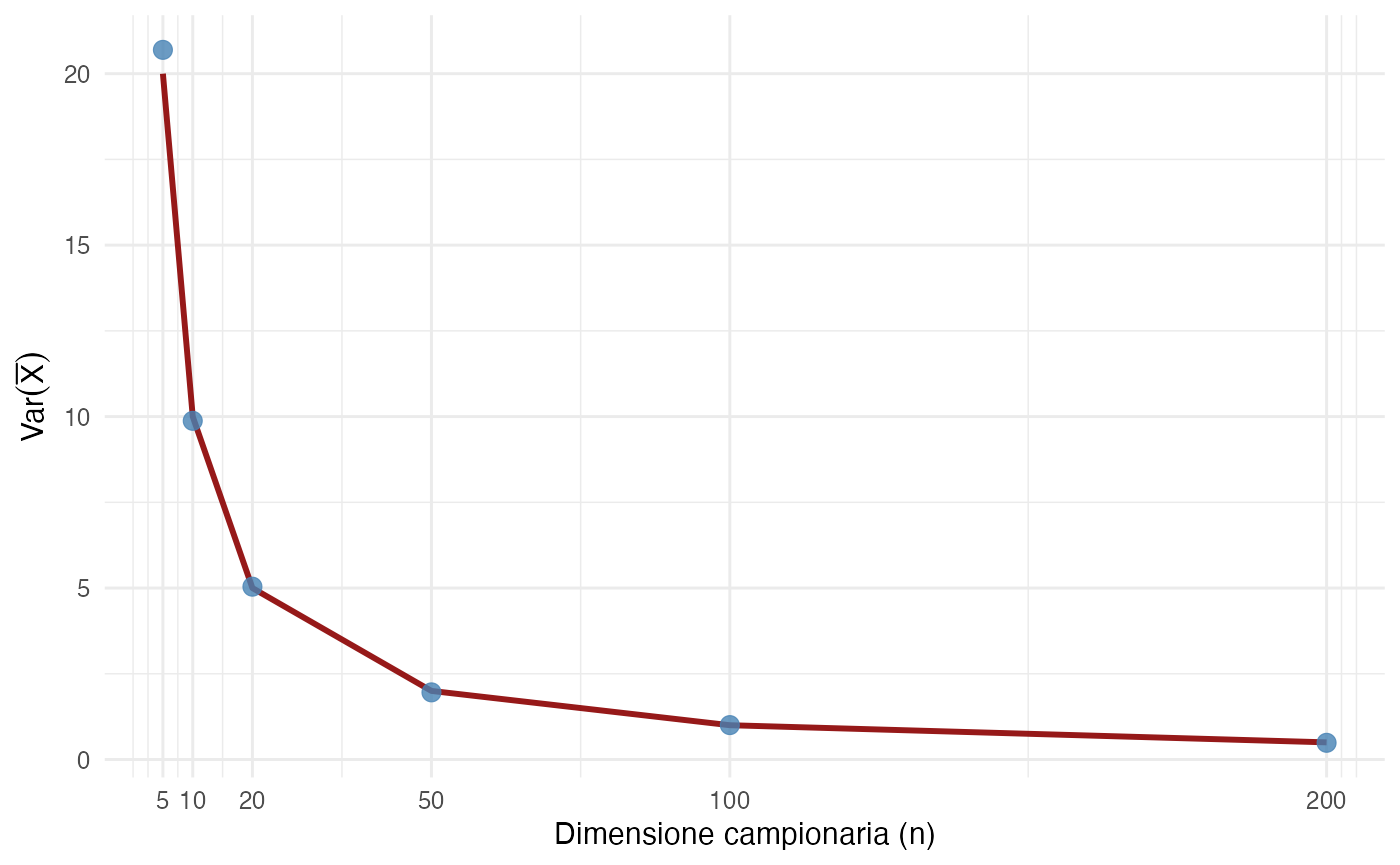
\includegraphics[width=0.85\linewidth,height=\textheight,keepaspectratio]{chapters/probability/08_expval_var_files/figure-pdf/fig-variance-sample-mean-1.png}

}

\caption{\label{fig-variance-sample-mean}La varianza della media
campionaria decresce come 1/n.~La simulazione (punti) conferma la
previsione teorica (linea).}

\end{figure}%

\section{Deviazione standard e
standardizzazione}\label{deviazione-standard-e-standardizzazione}

La varianza, essendo definita in termini di scarti quadratici, ha come
unità di misura il quadrato dell'unità della variabile originaria. Per
ottenere una misura di dispersione nella stessa scala dei dati, si usa
la \emph{deviazione standard}.

\begin{definition}[Deviazione
standard]\protect\hypertarget{def-standard-deviation}{}\label{def-standard-deviation}

La \emph{deviazione standard} di una variabile casuale \(X\) è: \[
\sigma_X = \text{SD}(X) = \sqrt{\text{Var}(X)}.
\]

\end{definition}

La deviazione standard rappresenta, approssimativamente, la ``distanza
tipica'' di un valore dalla media. Per molte distribuzioni simmetriche e
unimodali, la maggior parte dei valori si colloca entro una o due
deviazioni standard dalla media.

\subsection{Standardizzazione}\label{standardizzazione}

Qualsiasi variabile casuale può essere standardizzata sottraendo la
media e dividendo il risultato per la deviazione standard.

\begin{definition}[Variabile
standardizzata]\protect\hypertarget{def-standardization}{}\label{def-standardization}

Data una variabile casuale \(X\) con \(\mathbb{E}[X] = \mu\) e
\(\text{SD}(X) = \sigma\), la \emph{variabile standardizzata} è: \[
Z = \frac{X - \mu}{\sigma}.
\]

\end{definition}

La variabile standardizzata \(Z\) ha sempre \(\mathbb{E}[Z] = 0\) e
\(\text{Var}(Z) = 1\), indipendentemente dalla distribuzione originaria
di \(X\). Questo processo permette di confrontare variabili misurate su
scale diverse e di esprimere ogni valore in termini di ``quante
deviazioni standard'' esso disti dalla media.

\begin{tcolorbox}[enhanced jigsaw, arc=.35mm, breakable, colbacktitle=quarto-callout-note-color!10!white, opacityback=0, toprule=.15mm, rightrule=.15mm, colback=white, opacitybacktitle=0.6, leftrule=.75mm, coltitle=black, bottomtitle=1mm, left=2mm, toptitle=1mm, title=\textcolor{quarto-callout-note-color}{\faInfo}\hspace{0.5em}{Esempio: Standardizzazione dei punteggi QI}, titlerule=0mm, bottomrule=.15mm, colframe=quarto-callout-note-color-frame]

\subsection{Confronto tra scale
diverse}\label{confronto-tra-scale-diverse}

Il QI ha tradizionalmente \(\mu = 100\) e \(\sigma = 15\). Un punteggio
di 130 corrisponde a: \[
z = \frac{130 - 100}{15} = 2.0
\]

ovvero 2 deviazioni standard sopra la media.

Se un altro test cognitivo ha \(\mu = 50\) e \(\sigma = 10\), quale
punteggio corrisponde allo stesso livello relativo? \[
x = \mu + z \cdot \sigma = 50 + 2.0 \times 10 = 70.
\]

La standardizzazione permette di tradurre punteggi tra scale diverse
mantenendo il significato relativo.

\end{tcolorbox}

\section{Il teorema di Chebyshev}\label{il-teorema-di-chebyshev}

Una domanda naturale è: quanto della distribuzione cade entro un certo
numero di deviazioni standard dalla media? Il \emph{teorema di
Chebyshev} fornisce una risposta universale, valida per qualsiasi
distribuzione.

\begin{theorem}[Teorema di
Chebyshev]\protect\hypertarget{thm-chebyshev}{}\label{thm-chebyshev}

Per qualsiasi variabile casuale \(X\) con media \(\mu\) e deviazione
standard \(\sigma\), e per qualsiasi \(k > 0\): \[
P(|X - \mu| \geq k\sigma) \leq \frac{1}{k^2}.
\]

Equivalentemente: \[
P(|X - \mu| < k\sigma) \geq 1 - \frac{1}{k^2}.
\]

\end{theorem}

Il teorema fornisce un limite inferiore alla probabilità che una
variabile cada entro \(k\) deviazioni standard dalla media:

\begin{longtable}[]{@{}cc@{}}
\toprule\noalign{}
\(k\) & \(P(\|X - \mu\| < k\sigma) \geq\) \\
\midrule\noalign{}
\endhead
\bottomrule\noalign{}
\endlastfoot
1 & 0\% (limite triviale) \\
2 & 75\% \\
3 & 89\% \\
4 & 94\% \\
\end{longtable}

Questi limiti sono conservativi: per molte distribuzioni comuni (come la
normale), le probabilità effettive sono molto più alte. Tuttavia, il
teorema è valido universalmente, senza assumere nulla sulla forma della
distribuzione.

\begin{tcolorbox}[enhanced jigsaw, arc=.35mm, breakable, colbacktitle=quarto-callout-note-color!10!white, opacityback=0, toprule=.15mm, rightrule=.15mm, colback=white, opacitybacktitle=0.6, leftrule=.75mm, coltitle=black, bottomtitle=1mm, left=2mm, toptitle=1mm, title=\textcolor{quarto-callout-note-color}{\faInfo}\hspace{0.5em}{Esempio: Applicazione del teorema di Chebyshev}, titlerule=0mm, bottomrule=.15mm, colframe=quarto-callout-note-color-frame]

\subsection{Stima di probabilità}\label{stima-di-probabilituxe0}

Un test psicometrico ha media 100 e deviazione standard 15. Senza
conoscere la distribuzione esatta, possiamo affermare che almeno il 75\%
dei punteggi cade nell'intervallo: \[
[100 - 2 \times 15, 100 + 2 \times 15] = [70, 130].
\]

Per la distribuzione normale, la proporzione effettiva è circa
95\%---molto superiore al limite di Chebyshev, ma il teorema ci dà una
garanzia minima senza dover assumere la normalità.

\end{tcolorbox}

\section{Momenti di una
distribuzione}\label{momenti-di-una-distribuzione}

Il valore atteso e la varianza sono i primi due \textbf{momenti} di una
distribuzione, ovvero una famiglia di quantità che caratterizzano
completamente la forma della distribuzione sotto certe condizioni.

\begin{definition}[Momenti]\protect\hypertarget{def-moments}{}\label{def-moments}

Il \emph{momento di ordine \(r\)} di una variabile casuale \(X\) è: \[
\mathbb{E}[X^r] = \begin{cases}
\sum_i x_i^r \cdot p_X(x_i) & \text{(caso discreto)} \\
\int_{-\infty}^{+\infty} x^r \cdot f_X(x) \, dx & \text{(caso continuo)}
\end{cases}
\]

Il \emph{momento centrale di ordine \(r\)} è: \[
\mathbb{E}[(X - \mu)^r],
\] dove \(\mu = \mathbb{E}[X]\).

\end{definition}

Il momento di ordine 1 è il valore atteso. Il momento centrale di ordine
2 è la varianza. I momenti di ordine superiore catturano altre
caratteristiche della distribuzione: il terzo momento centrale
(opportunamente normalizzato) misura l'asimmetria, mentre il quarto
misura l'eccesso di curtosi, ovvero quanto le code sono pesanti rispetto
a una distribuzione normale.

\section*{Riflessioni conclusive}\label{riflessioni-conclusive-7}

\markright{Riflessioni conclusive}

Il valore atteso e la varianza sono gli strumenti fondamentali per
sintetizzare una distribuzione di probabilità. Il valore atteso
localizza il centro, ovvero il ``baricentro probabilistico'', mentre la
varianza quantifica la dispersione attorno a esso.

Le proprietà algebriche di queste quantità, ovvero la linearità del
valore atteso e l'additività della varianza per variabili indipendenti,
semplificano notevolmente i calcoli pratici e rivelano le strutture
profonde delle relazioni tra le variabili casuali. La proprietà per cui
la varianza della media campionaria decresce come \(1/n\) è alla base
dell'inferenza statistica e spiega perché i campioni più grandi
forniscono stime più affidabili.

Questi concetti troveranno immediata applicazione nei capitoli
successivi, in cui verranno studiate specifiche famiglie di
distribuzioni (Beta, Normale, Poisson e Binomiale) e verrà costruito
l'apparato formale dell'inferenza bayesiana. Il valore atteso del
parametro sotto la distribuzione a posteriori sarà la nostra stima
puntuale bayesiana, mentre la varianza a posteriori quantificherà
l'incertezza residua dopo l'osservazione dei dati.

\begin{tcolorbox}[enhanced jigsaw, arc=.35mm, breakable, colbacktitle=quarto-callout-note-color!10!white, opacityback=0, toprule=.15mm, rightrule=.15mm, colback=white, opacitybacktitle=0.6, leftrule=.75mm, coltitle=black, bottomtitle=1mm, left=2mm, toptitle=1mm, title=\textcolor{quarto-callout-note-color}{\faInfo}\hspace{0.5em}{Informazioni sull'ambiente di sviluppo}, titlerule=0mm, bottomrule=.15mm, colframe=quarto-callout-note-color-frame]

\begin{Shaded}
\begin{Highlighting}[]
\FunctionTok{sessionInfo}\NormalTok{()}
\CommentTok{\#\textgreater{} R version 4.5.2 (2025{-}10{-}31)}
\CommentTok{\#\textgreater{} Platform: aarch64{-}apple{-}darwin20}
\CommentTok{\#\textgreater{} Running under: macOS Tahoe 26.1}
\CommentTok{\#\textgreater{} }
\CommentTok{\#\textgreater{} Matrix products: default}
\CommentTok{\#\textgreater{} BLAS:   /System/Library/Frameworks/Accelerate.framework/Versions/A/Frameworks/vecLib.framework/Versions/A/libBLAS.dylib }
\CommentTok{\#\textgreater{} LAPACK: /Library/Frameworks/R.framework/Versions/4.5{-}arm64/Resources/lib/libRlapack.dylib;  LAPACK version 3.12.1}
\CommentTok{\#\textgreater{} }
\CommentTok{\#\textgreater{} locale:}
\CommentTok{\#\textgreater{} [1] C.UTF{-}8/UTF{-}8/C.UTF{-}8/C/C.UTF{-}8/C.UTF{-}8}
\CommentTok{\#\textgreater{} }
\CommentTok{\#\textgreater{} time zone: Europe/Rome}
\CommentTok{\#\textgreater{} tzcode source: internal}
\CommentTok{\#\textgreater{} }
\CommentTok{\#\textgreater{} attached base packages:}
\CommentTok{\#\textgreater{} [1] stats     graphics  grDevices utils     datasets  methods   base     }
\CommentTok{\#\textgreater{} }
\CommentTok{\#\textgreater{} other attached packages:}
\CommentTok{\#\textgreater{}  [1] pillar\_1.11.1         tinytable\_0.15.1      patchwork\_1.3.2      }
\CommentTok{\#\textgreater{}  [4] ggdist\_3.3.3          tidybayes\_3.0.7       bayesplot\_1.14.0     }
\CommentTok{\#\textgreater{}  [7] ggplot2\_4.0.1         reliabilitydiag\_0.2.1 priorsense\_1.2.0     }
\CommentTok{\#\textgreater{} [10] posterior\_1.6.1       loo\_2.8.0             rstan\_2.32.7         }
\CommentTok{\#\textgreater{} [13] StanHeaders\_2.32.10   brms\_2.23.0           Rcpp\_1.1.0           }
\CommentTok{\#\textgreater{} [16] sessioninfo\_1.2.3     conflicted\_1.2.0      janitor\_2.2.1        }
\CommentTok{\#\textgreater{} [19] matrixStats\_1.5.0     modelr\_0.1.11         tibble\_3.3.0         }
\CommentTok{\#\textgreater{} [22] dplyr\_1.1.4           tidyr\_1.3.1           rio\_1.2.4            }
\CommentTok{\#\textgreater{} [25] here\_1.0.2           }
\CommentTok{\#\textgreater{} }
\CommentTok{\#\textgreater{} loaded via a namespace (and not attached):}
\CommentTok{\#\textgreater{}  [1] svUnit\_1.0.8          tidyselect\_1.2.1      farver\_2.1.2         }
\CommentTok{\#\textgreater{}  [4] S7\_0.2.1              fastmap\_1.2.0         TH.data\_1.1{-}5        }
\CommentTok{\#\textgreater{}  [7] tensorA\_0.36.2.1      pacman\_0.5.1          digest\_0.6.39        }
\CommentTok{\#\textgreater{} [10] timechange\_0.3.0      estimability\_1.5.1    lifecycle\_1.0.4      }
\CommentTok{\#\textgreater{} [13] survival\_3.8{-}3        magrittr\_2.0.4        compiler\_4.5.2       }
\CommentTok{\#\textgreater{} [16] rlang\_1.1.6           tools\_4.5.2           yaml\_2.3.10          }
\CommentTok{\#\textgreater{} [19] knitr\_1.50            labeling\_0.4.3        bridgesampling\_1.2{-}1 }
\CommentTok{\#\textgreater{} [22] curl\_7.0.0            pkgbuild\_1.4.8        RColorBrewer\_1.1{-}3   }
\CommentTok{\#\textgreater{} [25] abind\_1.4{-}8           multcomp\_1.4{-}29       withr\_3.0.2          }
\CommentTok{\#\textgreater{} [28] purrr\_1.2.0           grid\_4.5.2            stats4\_4.5.2         }
\CommentTok{\#\textgreater{} [31] colorspace\_2.1{-}2      xtable\_1.8{-}4          inline\_0.3.21        }
\CommentTok{\#\textgreater{} [34] emmeans\_2.0.0         scales\_1.4.0          MASS\_7.3{-}65          }
\CommentTok{\#\textgreater{} [37] cli\_3.6.5             mvtnorm\_1.3{-}3         rmarkdown\_2.30       }
\CommentTok{\#\textgreater{} [40] ragg\_1.5.0            generics\_0.1.4        RcppParallel\_5.1.11{-}1}
\CommentTok{\#\textgreater{} [43] cachem\_1.1.0          stringr\_1.6.0         splines\_4.5.2        }
\CommentTok{\#\textgreater{} [46] parallel\_4.5.2        vctrs\_0.6.5           V8\_8.0.1             }
\CommentTok{\#\textgreater{} [49] Matrix\_1.7{-}4          sandwich\_3.1{-}1        jsonlite\_2.0.0       }
\CommentTok{\#\textgreater{} [52] arrayhelpers\_1.1{-}0    systemfonts\_1.3.1     glue\_1.8.0           }
\CommentTok{\#\textgreater{} [55] codetools\_0.2{-}20      distributional\_0.5.0  lubridate\_1.9.4      }
\CommentTok{\#\textgreater{} [58] stringi\_1.8.7         gtable\_0.3.6          QuickJSR\_1.8.1       }
\CommentTok{\#\textgreater{} [61] htmltools\_0.5.8.1     Brobdingnag\_1.2{-}9     R6\_2.6.1             }
\CommentTok{\#\textgreater{} [64] textshaping\_1.0.4     rprojroot\_2.1.1       evaluate\_1.0.5       }
\CommentTok{\#\textgreater{} [67] lattice\_0.22{-}7        backports\_1.5.0       memoise\_2.0.1        }
\CommentTok{\#\textgreater{} [70] broom\_1.0.10          snakecase\_0.11.1      rstantools\_2.5.0     }
\CommentTok{\#\textgreater{} [73] coda\_0.19{-}4.1         gridExtra\_2.3         nlme\_3.1{-}168         }
\CommentTok{\#\textgreater{} [76] checkmate\_2.3.3       xfun\_0.54             zoo\_1.8{-}14           }
\CommentTok{\#\textgreater{} [79] pkgconfig\_2.0.3}
\end{Highlighting}
\end{Shaded}

\end{tcolorbox}

\section*{Bibliografia}\label{bibliografia-5}

\markright{Bibliografia}

\chapter{Covarianza e correlazione}\label{sec-prob-cov-cor}

\section*{Introduzione}\label{introduzione-9}

\markright{Introduzione}

Nel Chapter~\ref{sec-prob-axioms-coherence} abbiamo costruito tabelle di
probabilità congiunta per rappresentare in modo coerente le nostre
credenze sui sistemi multivariati. Abbiamo visto che queste tabelle
costituiscono la rappresentazione più completa delle relazioni tra le
variabili: una volta specificata una distribuzione congiunta coerente,
tutte le altre quantità probabilistiche, come le distribuzioni
marginali, condizionate e le probabilità di eventi complessi, ne
derivano automaticamente attraverso operazioni di somma e
normalizzazione.

In questo capitolo ci poniamo una domanda pratica: come possiamo
riassumere in modo sintetico la struttura di dipendenza tra variabili
espressa da una distribuzione congiunta? La covarianza e la correlazione
forniscono indici numerici che catturano un aspetto specifico della
relazione tra variabili: la tendenza alla covariazione lineare. Dal
punto di vista bayesiano, questi indici sintetizzano in forma compatta
le informazioni sulla struttura delle nostre credenze codificate nella
distribuzione congiunta.

Prima di introdurre questi indici, estenderemo brevemente il framework
delle tabelle congiunte al caso continuo, mostrando come le stesse idee
si applichino quando le variabili assumono valori su scale numeriche
continue. Questa estensione è necessaria per comprendere appieno il
significato della covarianza e della correlazione, che trovano la loro
applicazione più naturale proprio nel contesto delle distribuzioni
continue.

\subsection*{Panoramica del capitolo}\label{panoramica-del-capitolo-8}

\begin{itemize}
\tightlist
\item
  Estensione al caso continuo: dalle tabelle alle densità congiunte.
\item
  Covarianza come misura epistemica della co-variazione lineare.
\item
  Correlazione come versione standardizzata della covarianza.
\item
  Proprietà matematiche e loro significato epistemico.
\item
  Il concetto di incorrelazione e la sua relazione con l'indipendenza.
\item
  Applicazioni nell'inferenza bayesiana.
\end{itemize}

\begin{tcolorbox}[enhanced jigsaw, arc=.35mm, breakable, colbacktitle=quarto-callout-tip-color!10!white, opacityback=0, toprule=.15mm, rightrule=.15mm, colback=white, opacitybacktitle=0.6, leftrule=.75mm, coltitle=black, bottomtitle=1mm, left=2mm, toptitle=1mm, title=\textcolor{quarto-callout-tip-color}{\faLightbulb}\hspace{0.5em}{Prerequisiti}, titlerule=0mm, bottomrule=.15mm, colframe=quarto-callout-tip-color-frame]

\begin{itemize}
\tightlist
\item
  Chapter~\ref{sec-prob-axioms-coherence}: assiomi e coerenza delle
  credenze.
\item
  Concetti di valore atteso e varianza.
\end{itemize}

\end{tcolorbox}

\begin{tcolorbox}[enhanced jigsaw, arc=.35mm, breakable, colbacktitle=quarto-callout-caution-color!10!white, opacityback=0, toprule=.15mm, rightrule=.15mm, colback=white, opacitybacktitle=0.6, leftrule=.75mm, coltitle=black, bottomtitle=1mm, left=2mm, toptitle=1mm, title=\textcolor{quarto-callout-caution-color}{\faFire}\hspace{0.5em}{Preparazione del Notebook}, titlerule=0mm, bottomrule=.15mm, colframe=quarto-callout-caution-color-frame]

\begin{Shaded}
\begin{Highlighting}[]
\NormalTok{here}\SpecialCharTok{::}\FunctionTok{here}\NormalTok{(}\StringTok{"code"}\NormalTok{, }\StringTok{"\_common.R"}\NormalTok{) }\SpecialCharTok{|\textgreater{}}
  \FunctionTok{source}\NormalTok{()}
\FunctionTok{library}\NormalTok{(MASS)}
\FunctionTok{library}\NormalTok{(viridis)}
\FunctionTok{library}\NormalTok{(ggExtra)}
\end{Highlighting}
\end{Shaded}

\end{tcolorbox}

\section{Dalle tabelle discrete alle densità
continue}\label{dalle-tabelle-discrete-alle-densituxe0-continue}

Nel Chapter~\ref{sec-prob-axioms-coherence} abbiamo lavorato con tabelle
congiunte 2×2 per rappresentare credenze su coppie di variabili binarie.
Questi stessi principi si estendono naturalmente a situazioni più
complesse: tabelle con più categorie quando le variabili hanno molti
livelli, e densità congiunte quando le variabili assumono valori su
scale continue.

\subsection{Tabelle con più
categorie}\label{tabelle-con-piuxf9-categorie}

Consideriamo un esempio tratto dalla letteratura psicologica: la
relazione tra ansia e prestazione cognitiva negli studenti universitari.
La ricerca indica spesso una relazione negativa tra questi fattori
(\citeproc{ref-eysenck2007anxiety}{Eysenck et al., 2007}). Codifichiamo
l'ansia in tre livelli (bassa, media, alta) e la prestazione in tre
livelli (insufficiente, sufficiente, buona).

La distribuzione congiunta che rappresenta le nostre credenze basate
sulla letteratura potrebbe assumere la seguente forma:

\begin{longtable}[]{@{}lllll@{}}
\toprule\noalign{}
& Ansia Bassa & Ansia Media & Ansia Alta & Marginale \\
\midrule\noalign{}
\endhead
\bottomrule\noalign{}
\endlastfoot
Insufficiente & 0.05 & 0.10 & 0.15 & 0.30 \\
Sufficiente & 0.15 & 0.20 & 0.10 & 0.45 \\
Buona & 0.10 & 0.10 & 0.05 & 0.25 \\
\textbf{Marginale} & 0.30 & 0.40 & 0.30 & 1.00 \\
\end{longtable}

Ogni cella rappresenta il nostro grado di credenza in una specifica
configurazione. Ad esempio, assegniamo una probabilità dello 0.20 alla
configurazione ``prestazione sufficiente con ansia media'', mentre
attribuiamo solo uno 0.05 alla configurazione ``buona prestazione con
alta ansia'', riflettendo quanto riportato dalla letteratura sulla
relazione negativa tra ansia e prestazione.

I principi rimangono gli stessi delle tabelle 2×2: le marginali si
ottengono sommando lungo le righe e le colonne, le condizionate si
ricavano dividendo per la marginale appropriata e la coerenza è
garantita dalla non negatività di tutte le celle e dalla somma totale
pari a uno.

\subsection{Il caso continuo: densità
congiunte}\label{il-caso-continuo-densituxe0-congiunte}

Quando le variabili sono continue, come i punteggi su scale
psicometriche, i tempi di reazione o le misure fisiologiche, la
distribuzione congiunta è rappresentata da una \emph{densità} \(f(x,y)\)
piuttosto che da probabilità discrete. L'interpretazione epistemica
rimane la stessa: la densità indica quanto riteniamo plausibile una
determinata regione dello spazio delle configurazioni possibili.

\begin{definition}[]\protect\hypertarget{def-joint-density}{}\label{def-joint-density}

Una \emph{densità congiunta} \(f(x,y)\) assegna a ogni configurazione
\((x,y)\) un valore che rappresenta la ``concentrazione di credenza'' in
quella regione. Per essere coerente, deve soddisfare:

\begin{enumerate}
\def\labelenumi{\arabic{enumi}.}
\item
  \textbf{Non-negatività}: \(f(x,y) \geq 0\) per ogni \((x,y)\).
\item
  \textbf{Normalizzazione}:
  \[\int_{-\infty}^{+\infty}\int_{-\infty}^{+\infty} f(x,y)\,dx\,dy = 1.\]
\end{enumerate}

\end{definition}

Come per le tabelle discrete, la densità congiunta contiene tutte le
informazioni sulle relazioni tra le variabili. Le densità marginali si
ottengono integrando su una delle variabili:

\[
f_X(x) = \int_{-\infty}^{+\infty} f(x,y) \, dy, \qquad f_Y(y) = \int_{-\infty}^{+\infty} f(x,y) \, dx.
\]

Le densità condizionate si ricavano dividendo la congiunta per la
marginale:

\[
f_{X \mid Y}(x \mid y) = \frac{f(x,y)}{f_Y(y)}.
\]

\subsection{Visualizzazione di una distribuzione congiunta
continua}\label{visualizzazione-di-una-distribuzione-congiunta-continua}

Per rendere più concreto il concetto di densità congiunta, consideriamo
nuovamente la relazione tra ansia e prestazione cognitiva, questa volta
modellata come distribuzione continua. Possiamo visualizzare la densità
come una mappa termica in cui i colori più caldi indicano le
configurazioni a cui attribuiamo maggiore probabilità.

\begin{center}
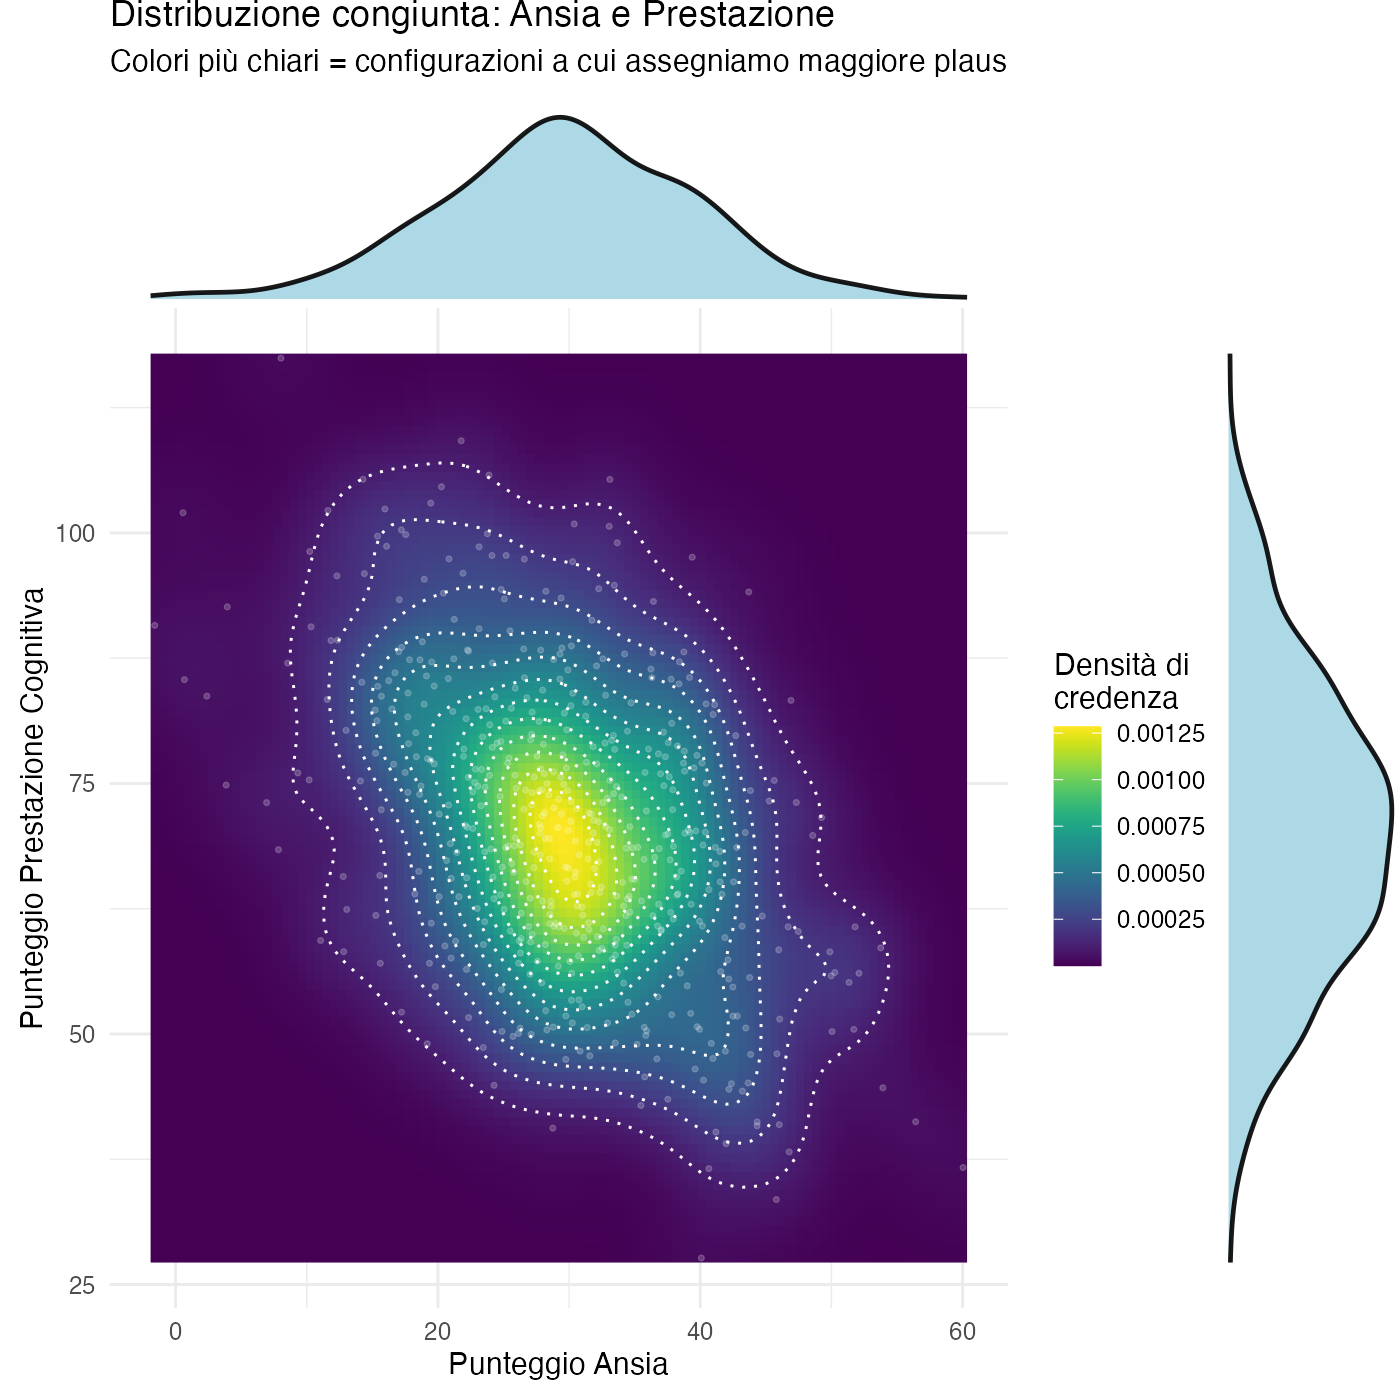
\includegraphics[width=0.85\linewidth,height=\textheight,keepaspectratio]{chapters/probability/10_cov_cor_files/figure-pdf/unnamed-chunk-2-1.png}
\end{center}

La visualizzazione rivela diversi aspetti della struttura delle nostre
credenze. La regione più chiara, situata nella parte centro-sinistra in
alto, rappresenta le configurazioni a cui attribuiamo la massima
credibilità: bassa ansia associata a buona prestazione. Le regioni più
scure, verso l'angolo in alto a destra, indicano configurazioni meno
plausibili: alta ansia con buona prestazione. L'orientamento ellittico
della distribuzione, inclinato verso il basso da sinistra a destra,
riflette la correlazione negativa che abbiamo incorporato nelle nostre
credenze sulla base della letteratura.

I grafici ai margini mostrano le densità marginali, ottenute proiettando
la distribuzione congiunta su ciascun asse. Queste rappresentano le
nostre credenze su ciascuna variabile singolarmente, quando non sono
condizionate dall'altra.

\begin{tcolorbox}[enhanced jigsaw, arc=.35mm, breakable, colbacktitle=quarto-callout-important-color!10!white, opacityback=0, toprule=.15mm, rightrule=.15mm, colback=white, opacitybacktitle=0.6, leftrule=.75mm, coltitle=black, bottomtitle=1mm, left=2mm, toptitle=1mm, title=\textcolor{quarto-callout-important-color}{\faExclamation}\hspace{0.5em}{Dalla distribuzione congiunta ai riassunti numerici}, titlerule=0mm, bottomrule=.15mm, colframe=quarto-callout-important-color-frame]

La distribuzione congiunta contiene tutte le informazioni sulle
relazioni tra le variabili. Tuttavia, comunicare un'intera distribuzione
può essere complesso. La covarianza e la correlazione sono riassunti
unidimensionali che:

\begin{itemize}
\tightlist
\item
  catturano l'aspetto lineare della relazione;
\item
  semplificano la comunicazione a un singolo numero;
\item
  perdono informazioni: possono esistere dipendenze non lineari con
  correlazione pari a zero.
\end{itemize}

Questi indici sono derivazioni utili ma parziali; la distribuzione
congiunta rimane la fonte primaria di informazione.

\end{tcolorbox}

Nel contesto del tuo capitolo, la sezione ``The sum and product rule'' è
concettualmente corretta, ma la formulazione inglese e la sintassi mista
con le virgole all'inizio di ogni riga rendono la lettura poco fluida
per uno studente di psicologia. Inoltre, l'idea delle regole di somma e
prodotto è già stata introdotta nei capitoli precedenti sulle tabelle
congiunte e sulle densità, quindi potrebbe essere utile integrarla in
maniera più naturale nel flusso del discorso, senza separarla come una
sezione a sé.

\subsection{Regole di somma e prodotto per le densità
congiunte}\label{regole-di-somma-e-prodotto-per-le-densituxe0-congiunte}

Come abbiamo visto con le tabelle congiunte discrete, è possibile
derivare le probabilità marginali e condizionate a partire dalla
distribuzione congiunta. Lo stesso principio vale quando le variabili
sono continue, sostituendo le somme con le integrali. Formalmente:

\begin{itemize}
\item
  \textbf{Regola di somma (marginalizzazione)} La densità marginale di
  \(Y\) si ottiene integrando la densità congiunta \(f_{X,Y}(x,y)\)
  rispetto a \(x\): \[
  f_Y(y) = \int_{-\infty}^{+\infty} f_{X,Y}(x,y) \,dx.
  \] Analogamente, la densità marginale di \(X\) è \[
  f_X(x) = \int_{-\infty}^{+\infty} f_{X,Y}(x,y) \,dy.
  \]
\item
  \textbf{Regola di prodotto (decomposizione in condizionale e
  marginale)} La distribuzione congiunta può essere espressa come
  prodotto della distribuzione marginale e di quella condizionale: \[
  f_{X,Y}(x,y) = f_{Y \mid X}(y \mid x) f_X(x) = f_{X \mid Y}(x \mid y) f_Y(y),
  \] dove \(f_{Y \mid X}(y \mid x)\) è la densità condizionata di \(Y\)
  dato \(X\).
\end{itemize}

Queste regole mostrano che conoscere la distribuzione congiunta equivale
a conoscere tutte le distribuzioni marginali e condizionate, e
viceversa: tutte le informazioni sulle relazioni tra variabili sono
contenute in \(f_{X,Y}(x,y)\). Da questo punto di vista, la covarianza e
la correlazione possono essere viste come sintesi numeriche che
riassumono parte di queste relazioni, in particolare la tendenza lineare
alla covariazione.

\section{Covarianza: misura della co-variazione
lineare}\label{covarianza-misura-della-co-variazione-lineare}

\subsection{Definizione e
interpretazione}\label{definizione-e-interpretazione}

La covarianza quantifica la tendenza di due variabili a variare insieme
in modo sistematico. Formalmente, misura il valore atteso del prodotto
delle deviazioni di ciascuna variabile dalla propria media.

\begin{definition}[]\protect\hypertarget{def-covariance}{}\label{def-covariance}

La \emph{covarianza} tra due variabili casuali \(X\) e \(Y\) è definita
come:

\[
\text{Cov}(X, Y) = \mathbb{E}\left[(X - \mathbb{E}[X])(Y - \mathbb{E}[Y])\right].
\]

Per variabili discrete con distribuzione congiunta \(p(x,y)\):

\[
\text{Cov}(X, Y) = \sum_{x}\sum_{y}(x - \mu_X)(y - \mu_Y)p(x, y),
\]

dove \(\mu_X = \mathbb{E}[X]\) e \(\mu_Y = \mathbb{E}[Y]\) sono i valori
attesi.

\end{definition}

L'interpretazione della covarianza emerge dalla struttura del prodotto
\((X - \mu_X)(Y - \mu_Y)\). Quando entrambe le variabili si trovano
dalla stessa parte delle rispettive medie, entrambe sopra o entrambe
sotto, il prodotto è positivo. Quando si trovano su lati opposti, il
prodotto è negativo. La covarianza è la media di questi prodotti,
ponderata secondo la distribuzione congiunta.

Una \textbf{covarianza positiva} che le configurazioni in cui entrambe
le variabili si discostano nella stessa direzione dalle rispettive medie
ricevono maggiore credibilità nella distribuzione congiunta. In altre
parole, crediamo che valori alti di \(X\) tendano ad accompagnarsi ai
valori alti di \(Y\) e viceversa.

Una \textbf{covarianza negativa} indica che le configurazioni in cui le
variabili deviano in direzioni opposte ricevono maggiore credibilità.
Crediamo che valori alti di \(X\) tendano ad accompagnarsi ai valori
bassi di \(Y\).

Una \textbf{covarianza nulla} indica l'assenza di una tendenza lineare
sistematica nella distribuzione della credenza. Le deviazioni dalla
media non mostrano un pattern prevedibile di co-variazione.

\subsection{Formula computazionale}\label{formula-computazionale}

La covarianza può essere calcolata in modo equivalente come:

\[
\text{Cov}(X, Y) = \mathbb{E}[XY] - \mathbb{E}[X]\mathbb{E}[Y].
\]

Questa formula confronta due quantità: il valore atteso del prodotto
sotto la distribuzione congiunta effettiva, indicato con
\(\mathbb{E}[XY]\), e il valore che otterremmo se le variabili fossero
indipendenti, indicato con \(\mathbb{E}[X]\mathbb{E}[Y]\). La differenza
misura quanto la distribuzione congiunta si discosti dall'indipendenza
in termini di co-variazione lineare.

\begin{tcolorbox}[enhanced jigsaw, arc=.35mm, breakable, colbacktitle=quarto-callout-note-color!10!white, opacityback=0, toprule=.15mm, rightrule=.15mm, colback=white, opacitybacktitle=0.6, leftrule=.75mm, coltitle=black, bottomtitle=1mm, left=2mm, toptitle=1mm, title=\textcolor{quarto-callout-note-color}{\faInfo}\hspace{0.5em}{Dimostrazione della formula computazionale}, titlerule=0mm, bottomrule=.15mm, colframe=quarto-callout-note-color-frame]

Partiamo dalla definizione:

\[
\text{Cov}(X, Y) = \mathbb{E}\bigl[(X - \mathbb{E}[X])(Y - \mathbb{E}[Y])\bigr]
\]

Espandiamo il prodotto:

\[
= \mathbb{E}[XY - X\mathbb{E}[Y] - \mathbb{E}[X]Y + \mathbb{E}[X]\mathbb{E}[Y]]
\]

Per la linearità del valore atteso e il fatto che \(\mathbb{E}[X]\) e
\(\mathbb{E}[Y]\) sono costanti:

\[
= \mathbb{E}[XY] - \mathbb{E}[X]\mathbb{E}[Y] - \mathbb{E}[X]\mathbb{E}[Y] + \mathbb{E}[X]\mathbb{E}[Y]
\]

Semplificando:

\[
\text{Cov}(X, Y) = \mathbb{E}[XY] - \mathbb{E}[X]\mathbb{E}[Y].
\]

\end{tcolorbox}

\subsection{Relazione con la varianza}\label{relazione-con-la-varianza}

La covarianza generalizza il concetto di varianza. Infatti, la varianza
di una variabile è semplicemente la covarianza di quella variabile con
se stessa:

\[
\mathbb{V}(X) = \text{Cov}(X, X) = \mathbb{E}[(X - \mathbb{E}[X])^2].
\]

Mentre la varianza misura quanto crediamo che \(X\) possa discostarsi
dal suo valore atteso, la covarianza misura quanto crediamo che le
deviazioni di \(X\) e \(Y\) tendano a muoversi insieme.

\section{Esempio: calcolo dalla tabella
congiunta}\label{esempio-calcolo-dalla-tabella-congiunta}

Applichiamo questi concetti alla tabella congiunta ansia-prestazione
introdotta in precedenza. Utilizzeremo la codifica numerica: prestazione
\(X \in \{0, 1, 2\}\) (insufficiente, sufficiente, buona) e ansia
\(Y \in \{0, 1, 2\}\) (bassa, media, alta).

\begin{Shaded}
\begin{Highlighting}[]
\CommentTok{\# Tabella congiunta}
\NormalTok{tab\_joint }\OtherTok{\textless{}{-}} \FunctionTok{matrix}\NormalTok{(}
  \FunctionTok{c}\NormalTok{(}\FloatTok{0.05}\NormalTok{, }\FloatTok{0.10}\NormalTok{, }\FloatTok{0.15}\NormalTok{,}
    \FloatTok{0.15}\NormalTok{, }\FloatTok{0.20}\NormalTok{, }\FloatTok{0.10}\NormalTok{,}
    \FloatTok{0.10}\NormalTok{, }\FloatTok{0.10}\NormalTok{, }\FloatTok{0.05}\NormalTok{),}
  \AttributeTok{nrow =} \DecValTok{3}\NormalTok{, }\AttributeTok{byrow =} \ConstantTok{TRUE}\NormalTok{,}
  \AttributeTok{dimnames =} \FunctionTok{list}\NormalTok{(}
    \AttributeTok{Prestazione =} \FunctionTok{c}\NormalTok{(}\StringTok{"Insufficiente (0)"}\NormalTok{, }\StringTok{"Sufficiente (1)"}\NormalTok{, }\StringTok{"Buona (2)"}\NormalTok{),}
    \AttributeTok{Ansia =} \FunctionTok{c}\NormalTok{(}\StringTok{"Bassa (0)"}\NormalTok{, }\StringTok{"Media (1)"}\NormalTok{, }\StringTok{"Alta (2)"}\NormalTok{)}
\NormalTok{  )}
\NormalTok{)}

\FunctionTok{cat}\NormalTok{(}\StringTok{"Distribuzione congiunta:}\SpecialCharTok{\textbackslash{}n}\StringTok{"}\NormalTok{)}
\CommentTok{\#\textgreater{} Distribuzione congiunta:}
\FunctionTok{print}\NormalTok{(tab\_joint)}
\CommentTok{\#\textgreater{}                    Ansia}
\CommentTok{\#\textgreater{} Prestazione         Bassa (0) Media (1) Alta (2)}
\CommentTok{\#\textgreater{}   Insufficiente (0)      0.05       0.1     0.15}
\CommentTok{\#\textgreater{}   Sufficiente (1)        0.15       0.2     0.10}
\CommentTok{\#\textgreater{}   Buona (2)              0.10       0.1     0.05}
\end{Highlighting}
\end{Shaded}

Il primo passo consiste nel calcolare i valori attesi dalle
distribuzioni marginali:

\begin{Shaded}
\begin{Highlighting}[]
\CommentTok{\# Valori delle variabili}
\NormalTok{val\_prest }\OtherTok{\textless{}{-}} \DecValTok{0}\SpecialCharTok{:}\DecValTok{2}
\NormalTok{val\_ansia }\OtherTok{\textless{}{-}} \DecValTok{0}\SpecialCharTok{:}\DecValTok{2}

\CommentTok{\# Distribuzioni marginali}
\NormalTok{marg\_prest }\OtherTok{\textless{}{-}} \FunctionTok{rowSums}\NormalTok{(tab\_joint)}
\NormalTok{marg\_ansia }\OtherTok{\textless{}{-}} \FunctionTok{colSums}\NormalTok{(tab\_joint)}

\CommentTok{\# Valori attesi}
\NormalTok{E\_X }\OtherTok{\textless{}{-}} \FunctionTok{sum}\NormalTok{(val\_prest }\SpecialCharTok{*}\NormalTok{ marg\_prest)}
\NormalTok{E\_Y }\OtherTok{\textless{}{-}} \FunctionTok{sum}\NormalTok{(val\_ansia }\SpecialCharTok{*}\NormalTok{ marg\_ansia)}

\FunctionTok{cat}\NormalTok{(}\StringTok{"}\SpecialCharTok{\textbackslash{}n}\StringTok{Distribuzioni marginali:}\SpecialCharTok{\textbackslash{}n}\StringTok{"}\NormalTok{)}
\CommentTok{\#\textgreater{} }
\CommentTok{\#\textgreater{} Distribuzioni marginali:}
\FunctionTok{cat}\NormalTok{(}\StringTok{"P(Prestazione):"}\NormalTok{, marg\_prest, }\StringTok{"}\SpecialCharTok{\textbackslash{}n}\StringTok{"}\NormalTok{)}
\CommentTok{\#\textgreater{} P(Prestazione): 0.3 0.45 0.25}
\FunctionTok{cat}\NormalTok{(}\StringTok{"P(Ansia):"}\NormalTok{, marg\_ansia, }\StringTok{"}\SpecialCharTok{\textbackslash{}n}\StringTok{"}\NormalTok{)}
\CommentTok{\#\textgreater{} P(Ansia): 0.3 0.4 0.3}
\FunctionTok{cat}\NormalTok{(}\StringTok{"}\SpecialCharTok{\textbackslash{}n}\StringTok{Valori attesi:}\SpecialCharTok{\textbackslash{}n}\StringTok{"}\NormalTok{)}
\CommentTok{\#\textgreater{} }
\CommentTok{\#\textgreater{} Valori attesi:}
\FunctionTok{cat}\NormalTok{(}\StringTok{"E[Prestazione] ="}\NormalTok{, }\FunctionTok{round}\NormalTok{(E\_X, }\DecValTok{3}\NormalTok{), }\StringTok{"}\SpecialCharTok{\textbackslash{}n}\StringTok{"}\NormalTok{)}
\CommentTok{\#\textgreater{} E[Prestazione] = 0.95}
\FunctionTok{cat}\NormalTok{(}\StringTok{"E[Ansia] ="}\NormalTok{, }\FunctionTok{round}\NormalTok{(E\_Y, }\DecValTok{3}\NormalTok{), }\StringTok{"}\SpecialCharTok{\textbackslash{}n}\StringTok{"}\NormalTok{)}
\CommentTok{\#\textgreater{} E[Ansia] = 1}
\end{Highlighting}
\end{Shaded}

Il valore atteso della prestazione, \(\mathbb{E}[X] = 0.95\),
rappresenta il ``centro di massa'' della nostra distribuzione di
credenze su questa variabile. Allo stesso modo, \(\mathbb{E}[Y] = 1.00\)
indica che la nostra credenza sull'ansia è centrata sul livello medio.

Ora calcoliamo \(\mathbb{E}[XY]\) sommando il prodotto \(xy\) pesato
dalla probabilità congiunta \(p(x,y)\):

\begin{Shaded}
\begin{Highlighting}[]
\CommentTok{\# Calcolo di E[XY]}
\NormalTok{E\_XY }\OtherTok{\textless{}{-}} \DecValTok{0}
\ControlFlowTok{for}\NormalTok{ (i }\ControlFlowTok{in} \DecValTok{1}\SpecialCharTok{:}\DecValTok{3}\NormalTok{) \{}
  \ControlFlowTok{for}\NormalTok{ (j }\ControlFlowTok{in} \DecValTok{1}\SpecialCharTok{:}\DecValTok{3}\NormalTok{) \{}
\NormalTok{    E\_XY }\OtherTok{\textless{}{-}}\NormalTok{ E\_XY }\SpecialCharTok{+}\NormalTok{ val\_prest[i] }\SpecialCharTok{*}\NormalTok{ val\_ansia[j] }\SpecialCharTok{*}\NormalTok{ tab\_joint[i, j]}
\NormalTok{  \}}
\NormalTok{\}}

\FunctionTok{cat}\NormalTok{(}\StringTok{"E[XY] ="}\NormalTok{, }\FunctionTok{round}\NormalTok{(E\_XY, }\DecValTok{3}\NormalTok{), }\StringTok{"}\SpecialCharTok{\textbackslash{}n}\StringTok{"}\NormalTok{)}
\CommentTok{\#\textgreater{} E[XY] = 0.8}
\end{Highlighting}
\end{Shaded}

Infine, applichiamo la formula computazionale:

\begin{Shaded}
\begin{Highlighting}[]
\CommentTok{\# Covarianza}
\NormalTok{Cov\_XY }\OtherTok{\textless{}{-}}\NormalTok{ E\_XY }\SpecialCharTok{{-}}\NormalTok{ E\_X }\SpecialCharTok{*}\NormalTok{ E\_Y}

\FunctionTok{cat}\NormalTok{(}\StringTok{"}\SpecialCharTok{\textbackslash{}n}\StringTok{Covarianza:}\SpecialCharTok{\textbackslash{}n}\StringTok{"}\NormalTok{)}
\CommentTok{\#\textgreater{} }
\CommentTok{\#\textgreater{} Covarianza:}
\FunctionTok{cat}\NormalTok{(}\StringTok{"Cov(X,Y) = E[XY] {-} E[X]·E[Y]}\SpecialCharTok{\textbackslash{}n}\StringTok{"}\NormalTok{)}
\CommentTok{\#\textgreater{} Cov(X,Y) = E[XY] {-} E[X]·E[Y]}
\FunctionTok{cat}\NormalTok{(}\StringTok{"         ="}\NormalTok{, }\FunctionTok{round}\NormalTok{(E\_XY, }\DecValTok{3}\NormalTok{), }\StringTok{"{-}"}\NormalTok{, }\FunctionTok{round}\NormalTok{(E\_X, }\DecValTok{3}\NormalTok{), }\StringTok{"×"}\NormalTok{, }\FunctionTok{round}\NormalTok{(E\_Y, }\DecValTok{3}\NormalTok{), }\StringTok{"}\SpecialCharTok{\textbackslash{}n}\StringTok{"}\NormalTok{)}
\CommentTok{\#\textgreater{}          = 0.8 {-} 0.95 × 1}
\FunctionTok{cat}\NormalTok{(}\StringTok{"         ="}\NormalTok{, }\FunctionTok{round}\NormalTok{(Cov\_XY, }\DecValTok{3}\NormalTok{), }\StringTok{"}\SpecialCharTok{\textbackslash{}n}\StringTok{"}\NormalTok{)}
\CommentTok{\#\textgreater{}          = {-}0.15}
\end{Highlighting}
\end{Shaded}

La covarianza negativa (\(\text{Cov}(X,Y) = -0.15\)) riflette la
struttura delle nostre credenze: nella tabella congiunta, abbiamo
assegnato una probabilità maggiore alle configurazioni in cui l'alta
ansia si accompagna a bassa prestazione (cella in alto a destra: 0.15)
rispetto alle configurazioni in cui l'alta ansia si accompagna a buona
prestazione (cella in basso a destra: 0.05). Questo pattern di credenze
produce la covarianza negativa osservata.

\section{Correlazione: covarianza
standardizzata}\label{correlazione-covarianza-standardizzata}

\subsection{Il problema delle unità di
misura}\label{il-problema-delle-unituxe0-di-misura}

La covarianza presenta un limite pratico: il suo valore numerico dipende
dalle unità di misura delle variabili. Se misurassimo l'ansia su una
scala da 0 a 100 invece che da 0 a 2, la covarianza cambierebbe di un
fattore 50, anche se la struttura delle nostre credenze sulla relazione
rimanesse identica. Ciò rende difficile il confronto delle covarianze
calcolate su variabili con scale diverse.

La correlazione risolve questo problema standardizzando la covarianza
rispetto alla variabilità delle singole variabili.

\begin{definition}[]\protect\hypertarget{def-correlation}{}\label{def-correlation}

Il \emph{coefficiente di correlazione} (o correlazione di Pearson) tra
\(X\) e \(Y\) è definito come:

\[
\rho(X,Y) = \frac{\text{Cov}(X,Y)}{\sqrt{\mathbb{V}(X) \cdot \mathbb{V}(Y)}} = \frac{\text{Cov}(X,Y)}{\sigma_X \sigma_Y}
\]

dove \(\sigma_X\) e \(\sigma_Y\) sono le deviazioni standard delle due
variabili.

\end{definition}

La correlazione è la covarianza ``normalizzata'' dalle deviazioni
standard. Misura la forza della relazione lineare su una scala
standardizzata compresa tra \(-1\) e \(+1\), indipendentemente dalle
unità di misura originali.

\subsection{Proprietà fondamentali}\label{proprietuxe0-fondamentali-1}

La correlazione possiede proprietà che ne facilitano l'interpretazione:

\begin{enumerate}
\def\labelenumi{\arabic{enumi}.}
\item
  \textbf{Limitatezza}: \(-1 \leq \rho(X,Y) \leq 1\) sempre.
\item
  \textbf{Invarianza per trasformazioni lineari}: se \(a > 0\) e
  \(b > 0\), allora \(\rho(aX + c, bY + d) = \rho(X, Y)\). La
  correlazione non cambia se rescaliamo o trasliamo le variabili.
\item
  \textbf{Valori estremi}:

  \begin{itemize}
  \tightlist
  \item
    \(\rho = +1\) indica una relazione lineare perfetta positiva:
    \(Y = a + bX\) con \(b > 0\);
  \item
    \(\rho = -1\) indica una relazione lineare perfetta negativa:
    \(Y = a + bX\) con \(b < 0\);
  \item
    \(\rho = 0\) indica l'assenza di relazione lineare (incorrelazione).
  \end{itemize}
\end{enumerate}

\subsection{Calcolo per l'esempio
ansia-prestazione}\label{calcolo-per-lesempio-ansia-prestazione}

\begin{Shaded}
\begin{Highlighting}[]
\CommentTok{\# Calcolo delle varianze}
\NormalTok{Var\_X }\OtherTok{\textless{}{-}} \FunctionTok{sum}\NormalTok{(val\_prest}\SpecialCharTok{\^{}}\DecValTok{2} \SpecialCharTok{*}\NormalTok{ marg\_prest) }\SpecialCharTok{{-}}\NormalTok{ E\_X}\SpecialCharTok{\^{}}\DecValTok{2}
\NormalTok{Var\_Y }\OtherTok{\textless{}{-}} \FunctionTok{sum}\NormalTok{(val\_ansia}\SpecialCharTok{\^{}}\DecValTok{2} \SpecialCharTok{*}\NormalTok{ marg\_ansia) }\SpecialCharTok{{-}}\NormalTok{ E\_Y}\SpecialCharTok{\^{}}\DecValTok{2}

\CommentTok{\# Correlazione}
\NormalTok{rho\_XY }\OtherTok{\textless{}{-}}\NormalTok{ Cov\_XY }\SpecialCharTok{/} \FunctionTok{sqrt}\NormalTok{(Var\_X }\SpecialCharTok{*}\NormalTok{ Var\_Y)}

\FunctionTok{cat}\NormalTok{(}\StringTok{"Varianze:}\SpecialCharTok{\textbackslash{}n}\StringTok{"}\NormalTok{)}
\CommentTok{\#\textgreater{} Varianze:}
\FunctionTok{cat}\NormalTok{(}\StringTok{"Var(X) ="}\NormalTok{, }\FunctionTok{round}\NormalTok{(Var\_X, }\DecValTok{4}\NormalTok{), }\StringTok{"}\SpecialCharTok{\textbackslash{}n}\StringTok{"}\NormalTok{)}
\CommentTok{\#\textgreater{} Var(X) = 0.547}
\FunctionTok{cat}\NormalTok{(}\StringTok{"Var(Y) ="}\NormalTok{, }\FunctionTok{round}\NormalTok{(Var\_Y, }\DecValTok{4}\NormalTok{), }\StringTok{"}\SpecialCharTok{\textbackslash{}n}\StringTok{"}\NormalTok{)}
\CommentTok{\#\textgreater{} Var(Y) = 0.6}
\FunctionTok{cat}\NormalTok{(}\StringTok{"}\SpecialCharTok{\textbackslash{}n}\StringTok{Deviazioni standard:}\SpecialCharTok{\textbackslash{}n}\StringTok{"}\NormalTok{)}
\CommentTok{\#\textgreater{} }
\CommentTok{\#\textgreater{} Deviazioni standard:}
\FunctionTok{cat}\NormalTok{(}\StringTok{"σ\_X ="}\NormalTok{, }\FunctionTok{round}\NormalTok{(}\FunctionTok{sqrt}\NormalTok{(Var\_X), }\DecValTok{4}\NormalTok{), }\StringTok{"}\SpecialCharTok{\textbackslash{}n}\StringTok{"}\NormalTok{)}
\CommentTok{\#\textgreater{} σ\_X = 0.74}
\FunctionTok{cat}\NormalTok{(}\StringTok{"σ\_Y ="}\NormalTok{, }\FunctionTok{round}\NormalTok{(}\FunctionTok{sqrt}\NormalTok{(Var\_Y), }\DecValTok{4}\NormalTok{), }\StringTok{"}\SpecialCharTok{\textbackslash{}n}\StringTok{"}\NormalTok{)}
\CommentTok{\#\textgreater{} σ\_Y = 0.775}
\FunctionTok{cat}\NormalTok{(}\StringTok{"}\SpecialCharTok{\textbackslash{}n}\StringTok{Correlazione:}\SpecialCharTok{\textbackslash{}n}\StringTok{"}\NormalTok{)}
\CommentTok{\#\textgreater{} }
\CommentTok{\#\textgreater{} Correlazione:}
\FunctionTok{cat}\NormalTok{(}\StringTok{"ρ(X,Y) ="}\NormalTok{, }\FunctionTok{round}\NormalTok{(rho\_XY, }\DecValTok{3}\NormalTok{), }\StringTok{"}\SpecialCharTok{\textbackslash{}n}\StringTok{"}\NormalTok{)}
\CommentTok{\#\textgreater{} ρ(X,Y) = {-}0.262}
\end{Highlighting}
\end{Shaded}

Il valore \(\rho(X,Y) \approx -0.26\) indica una relazione lineare
negativa di intensità moderata nella nostra distribuzione di credenze.
L'interpretazione è triplice: la \textbf{direzione negativa} conferma
che nelle nostre credenze livelli alti di ansia tendono ad associarsi a
livelli bassi di prestazione; l'\textbf{intensità moderata} (circa 0.26
in valore assoluto) indica che la relazione non è perfetta e che c'è una
sostanziale variabilità residua; la \textbf{natura lineare} dell'indice
ci ricorda che stiamo catturando solo la componente lineare della
relazione.

\subsection{Linee guida
interpretative}\label{linee-guida-interpretative}

Le convenzioni proposte da Cohen (1988) forniscono un quadro di
riferimento per l'interpretazione pratica della forza di una
correlazione:

\begin{itemize}
\tightlist
\item
  \(|\rho| < 0.3\): correlazione di entità modesta;
\item
  \(0.3 \leq |\rho| < 0.5\): correlazione di entità moderata;
\item
  \(|\rho| \geq 0.5\): correlazione di entità sostanziale.
\end{itemize}

Queste soglie hanno un carattere puramente indicativo e la loro
rilevanza sostanziale va valutata alla luce del contesto di ricerca
specifico. Nel nostro esempio, un valore di \(|\rho| = 0,26\) si colloca
al confine tra le categorie ``modesta'' e ``moderata''. È importante
sottolineare che un'associazione di questa entità può comunque avere una
notevole rilevanza psicologica, soprattutto considerando che i costrutti
psicologici sono solitamente influenzati da una molteplicità di fattori,
che le misure utilizzate sono inevitabilmente soggette a errore di
misurazione e che la relazione osservata potrebbe essere moderata da
altre variabili non incluse nel modello analitico.

\section{Proprietà matematiche della
covarianza}\label{proprietuxe0-matematiche-della-covarianza}

Le proprietà matematiche della covarianza hanno implicazioni pratiche
importanti per l'analisi dei dati psicologici.

\begin{theorem}[Proprietà della
covarianza]\protect\hypertarget{thm-cov-properties}{}\label{thm-cov-properties}

~

\begin{enumerate}
\def\labelenumi{\arabic{enumi}.}
\item
  \textbf{Simmetria}: \(\text{Cov}(X, Y) = \text{Cov}(Y, X).\)
\item
  \textbf{Covarianza con costante}: \(\text{Cov}(c, X) = 0\) per ogni
  costante \(c\).
\item
  \textbf{Linearità}:
  \(\text{Cov}(aX, bY) = ab \cdot \text{Cov}(X, Y).\)
\item
  \textbf{Additività}:
  \(\text{Cov}(X + Y, Z) = \text{Cov}(X, Z) + \text{Cov}(Y, Z).\)
\item
  \textbf{Varianza della somma}:
  \[\mathbb{V}(X + Y) = \mathbb{V}(X) + \mathbb{V}(Y) + 2\text{Cov}(X, Y).\]
\end{enumerate}

\end{theorem}

La \textbf{simmetria} riflette il fatto che la co-variazione è una
proprietà della relazione, non di una variabile in particolare. La
\textbf{covarianza nulla con costanti} deriva dal fatto che le costanti
non variano e quindi non possono co-variare con nulla.

Merita particolare attenzione la proprietà della \textbf{varianza della
somma}. Quando si combinano due variabili incerte, l'incertezza totale
non è semplicemente la somma delle incertezze individuali, ma dipende
anche dal modo in cui le variabili covariano. Se la covarianza è
positiva, le fluttuazioni tendono ad amplificarsi a vicenda e
l'incertezza totale aumenta oltre la somma delle incertezze individuali.
Se la covarianza è negativa, invece, le fluttuazioni tendono a
compensarsi e l'incertezza totale si riduce.

\subsection{Applicazione: costrutti psicologici
multidimensionali}\label{applicazione-costrutti-psicologici-multidimensionali}

La proprietà della varianza della somma trova applicazione nella
modellizzazione di costrutti psicologici complessi che risultano dalla
combinazione di più dimensioni.

\begin{Shaded}
\begin{Highlighting}[]
\CommentTok{\# Due dimensioni del benessere psicologico}
\NormalTok{sigma\_emotivo }\OtherTok{\textless{}{-}} \FloatTok{0.4}  \CommentTok{\# Variabilità benessere emotivo}
\NormalTok{sigma\_sociale }\OtherTok{\textless{}{-}} \FloatTok{0.3}  \CommentTok{\# Variabilità benessere sociale}
\NormalTok{rho\_psico }\OtherTok{\textless{}{-}} \FloatTok{0.6}      \CommentTok{\# Correlazione tra dimensioni}

\CommentTok{\# Pesi delle componenti nel costrutto complessivo}
\NormalTok{w\_emotivo }\OtherTok{\textless{}{-}} \FloatTok{0.6}
\NormalTok{w\_sociale }\OtherTok{\textless{}{-}} \FloatTok{0.4}

\CommentTok{\# Varianza del benessere psicologico complessivo}
\NormalTok{Var\_benessere }\OtherTok{\textless{}{-}}\NormalTok{ w\_emotivo}\SpecialCharTok{\^{}}\DecValTok{2} \SpecialCharTok{*}\NormalTok{ sigma\_emotivo}\SpecialCharTok{\^{}}\DecValTok{2} \SpecialCharTok{+} 
\NormalTok{                 w\_sociale}\SpecialCharTok{\^{}}\DecValTok{2} \SpecialCharTok{*}\NormalTok{ sigma\_sociale}\SpecialCharTok{\^{}}\DecValTok{2} \SpecialCharTok{+} 
                 \DecValTok{2} \SpecialCharTok{*}\NormalTok{ w\_emotivo }\SpecialCharTok{*}\NormalTok{ w\_sociale }\SpecialCharTok{*}\NormalTok{ rho\_psico }\SpecialCharTok{*}\NormalTok{ sigma\_emotivo }\SpecialCharTok{*}\NormalTok{ sigma\_sociale}

\NormalTok{sigma\_benessere }\OtherTok{\textless{}{-}} \FunctionTok{sqrt}\NormalTok{(Var\_benessere)}

\FunctionTok{cat}\NormalTok{(}\StringTok{"Variabilità benessere emotivo:"}\NormalTok{, sigma\_emotivo, }\StringTok{"}\SpecialCharTok{\textbackslash{}n}\StringTok{"}\NormalTok{)}
\CommentTok{\#\textgreater{} Variabilità benessere emotivo: 0.4}
\FunctionTok{cat}\NormalTok{(}\StringTok{"Variabilità benessere sociale:"}\NormalTok{, sigma\_sociale, }\StringTok{"}\SpecialCharTok{\textbackslash{}n}\StringTok{"}\NormalTok{)}
\CommentTok{\#\textgreater{} Variabilità benessere sociale: 0.3}
\FunctionTok{cat}\NormalTok{(}\StringTok{"Correlazione tra dimensioni:"}\NormalTok{, rho\_psico, }\StringTok{"}\SpecialCharTok{\textbackslash{}n}\StringTok{"}\NormalTok{)}
\CommentTok{\#\textgreater{} Correlazione tra dimensioni: 0.6}
\FunctionTok{cat}\NormalTok{(}\StringTok{"}\SpecialCharTok{\textbackslash{}n}\StringTok{Variabilità benessere complessivo:"}\NormalTok{, }\FunctionTok{round}\NormalTok{(sigma\_benessere, }\DecValTok{3}\NormalTok{), }\StringTok{"}\SpecialCharTok{\textbackslash{}n}\StringTok{"}\NormalTok{)}
\CommentTok{\#\textgreater{} }
\CommentTok{\#\textgreater{} Variabilità benessere complessivo: 0.326}
\end{Highlighting}
\end{Shaded}

L'integrazione di dimensioni correlate ma distinte produce una
variabilità complessiva che riflette non solo le incertezze individuali
ma anche la loro tendenza a co-variare. Nel caso di correlazione
positiva, come in questo esempio, le fluttuazioni delle due dimensioni
tendono a muoversi nella stessa direzione, amplificando la variabilità
del costrutto complessivo.

\section{Incorrelazione e
indipendenza}\label{incorrelazione-e-indipendenza}

\subsection{Definizione di
incorrelazione}\label{definizione-di-incorrelazione}

Due variabili si dicono \emph{incorrelate} (o linearmente indipendenti)
quando la loro covarianza è nulla:

\[
\text{Cov}(X, Y) = 0 \quad \Leftrightarrow \quad \rho(X, Y) = 0.
\]

Equivalentemente, si ha che
\(\mathbb{E}[XY] = \mathbb{E}[X]\mathbb{E}[Y]\), ovvero il valore atteso
del prodotto coincide con il prodotto dei valori attesi, come accadrebbe
se le variabili fossero indipendenti.

L'incorrelazione indica che non esiste una tendenza lineare sistematica
nella distribuzione delle credenze. Conoscere che \(X\) devia dalla sua
media non fornisce informazioni sulla direzione in cui \(Y\) potrebbe
deviare dalla propria.

\subsection{La distinzione cruciale: incorrelazione non implica
indipendenza}\label{la-distinzione-cruciale-incorrelazione-non-implica-indipendenza}

Una delle trappole concettuali più importanti nella statistica riguarda
la relazione tra incorrelazione e indipendenza.

\begin{tcolorbox}[enhanced jigsaw, arc=.35mm, breakable, colbacktitle=quarto-callout-important-color!10!white, opacityback=0, toprule=.15mm, rightrule=.15mm, colback=white, opacitybacktitle=0.6, leftrule=.75mm, coltitle=black, bottomtitle=1mm, left=2mm, toptitle=1mm, title=\textcolor{quarto-callout-important-color}{\faExclamation}\hspace{0.5em}{Relazione asimmetrica}, titlerule=0mm, bottomrule=.15mm, colframe=quarto-callout-important-color-frame]

\textbf{L'indipendenza implica l'incorrelazione}: se \(X\) e \(Y\) sono
indipendenti (cioè \(p(x,y) = p(x) \cdot p(y)\)), allora necessariamente
\(\text{Cov}(X,Y) = 0\).

\textbf{Ma l'incorrelazione NON implica l'indipendenza}: possono
esistere variabili con \(\text{Cov}(X,Y) = 0\) che sono fortemente
dipendenti.

\end{tcolorbox}

Perché questa asimmetria? La covarianza cattura esclusivamente la
\emph{relazione lineare}. Possono esistere relazioni non lineari molto
forti che non producono alcuna covarianza.

\subsection{Esempio: relazione quadratica con correlazione
zero}\label{esempio-relazione-quadratica-con-correlazione-zero}

\begin{Shaded}
\begin{Highlighting}[]
\FunctionTok{set.seed}\NormalTok{(}\DecValTok{42}\NormalTok{)}
\NormalTok{n }\OtherTok{\textless{}{-}} \DecValTok{1000}
\NormalTok{X }\OtherTok{\textless{}{-}} \FunctionTok{runif}\NormalTok{(n, }\SpecialCharTok{{-}}\DecValTok{2}\NormalTok{, }\DecValTok{2}\NormalTok{)}
\NormalTok{Y }\OtherTok{\textless{}{-}}\NormalTok{ X}\SpecialCharTok{\^{}}\DecValTok{2} \SpecialCharTok{+} \FunctionTok{rnorm}\NormalTok{(n, }\DecValTok{0}\NormalTok{, }\FloatTok{0.3}\NormalTok{)}

\FunctionTok{cat}\NormalTok{(}\StringTok{"Correlazione:"}\NormalTok{, }\FunctionTok{round}\NormalTok{(}\FunctionTok{cor}\NormalTok{(X, Y), }\DecValTok{3}\NormalTok{), }\StringTok{"}\SpecialCharTok{\textbackslash{}n}\StringTok{"}\NormalTok{)}
\CommentTok{\#\textgreater{} Correlazione: {-}0.013}

\CommentTok{\# Visualizzazione}
\FunctionTok{ggplot}\NormalTok{(}\FunctionTok{data.frame}\NormalTok{(}\AttributeTok{X =}\NormalTok{ X, }\AttributeTok{Y =}\NormalTok{ Y), }\FunctionTok{aes}\NormalTok{(}\AttributeTok{x =}\NormalTok{ X, }\AttributeTok{y =}\NormalTok{ Y)) }\SpecialCharTok{+}
  \FunctionTok{geom\_point}\NormalTok{(}\AttributeTok{alpha =} \FloatTok{0.5}\NormalTok{, }\AttributeTok{color =} \StringTok{"steelblue"}\NormalTok{) }\SpecialCharTok{+}
  \FunctionTok{labs}\NormalTok{(}
    \AttributeTok{title =} \StringTok{"Relazione non lineare con correlazione ≈ 0"}\NormalTok{,}
    \AttributeTok{subtitle =} \StringTok{"Le variabili sono fortemente dipendenti ma incorrelate"}\NormalTok{,}
    \AttributeTok{x =} \StringTok{"X"}\NormalTok{, }
    \AttributeTok{y =} \StringTok{"Y"}
\NormalTok{  ) }\SpecialCharTok{+}
  \FunctionTok{theme\_minimal}\NormalTok{()}
\end{Highlighting}
\end{Shaded}

\begin{center}
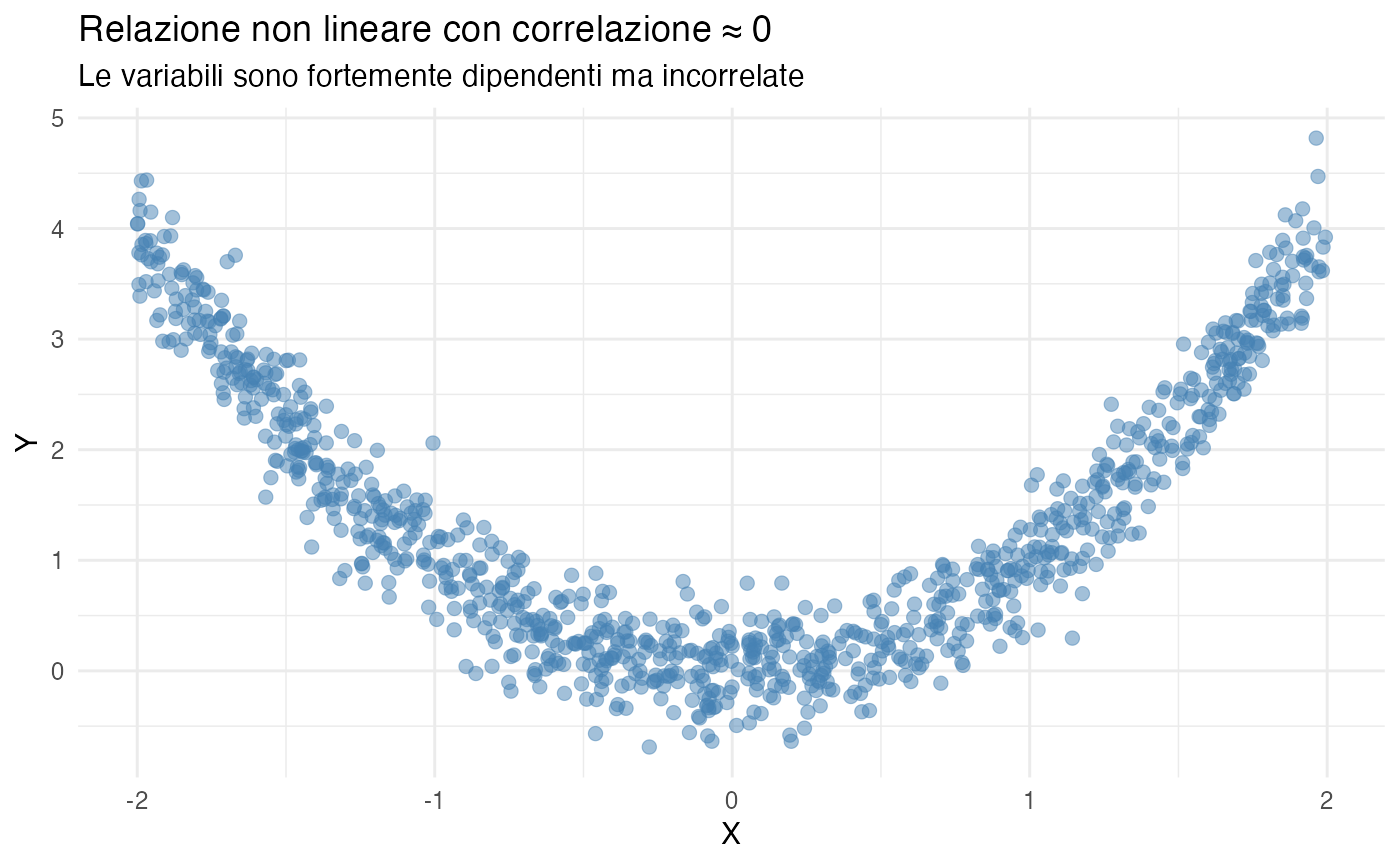
\includegraphics[width=0.85\linewidth,height=\textheight,keepaspectratio]{chapters/probability/10_cov_cor_files/figure-pdf/unnamed-chunk-9-1.png}
\end{center}

La figura mostra un caso paradigmatico: \(Y\) è completamente
determinato da \(X\) (a meno di un piccolo rumore), quindi le variabili
sono fortemente dipendenti. Tuttavia, la correlazione è essenzialmente
zero perché la relazione è quadratica e non lineare. La distribuzione
congiunta ha una struttura complessa, a forma di parabola, che la
correlazione non riesce a cogliere.

L'implicazione pratica è chiara: prima di concludere che due variabili
non sono associate, è necessario visualizzare la loro distribuzione
congiunta o lo scatterplot dei dati. Una correlazione pari a zero,
infatti, non garantisce l'assenza di relazione.

\section{Covarianza nell'inferenza
bayesiana}\label{covarianza-nellinferenza-bayesiana}

Nell'inferenza bayesiana, la covarianza assume un ruolo che va oltre la
semplice descrizione dei dati. Infatti, essa caratterizza anche le
nostre credenze sui parametri del modello in diversi stadi dell'analisi.

\subsection{Covarianza a priori}\label{covarianza-a-priori}

Prima di osservare i dati, è possibile specificare una distribuzione a
priori sui parametri che includa una struttura di covarianza. Questa
specifica riflette la nostra conoscenza pregressa sulle relazioni tra i
parametri.

\begin{Shaded}
\begin{Highlighting}[]
\CommentTok{\# Prior multivariata normale per due parametri}
\NormalTok{mu\_prior }\OtherTok{\textless{}{-}} \FunctionTok{c}\NormalTok{(}\DecValTok{0}\NormalTok{, }\DecValTok{0}\NormalTok{)}
\NormalTok{Sigma\_prior }\OtherTok{\textless{}{-}} \FunctionTok{matrix}\NormalTok{(}\FunctionTok{c}\NormalTok{(}\DecValTok{1}\NormalTok{, }\FloatTok{0.7}\NormalTok{, }\FloatTok{0.7}\NormalTok{, }\DecValTok{1}\NormalTok{), }\AttributeTok{nrow =} \DecValTok{2}\NormalTok{)}

\CommentTok{\# Simuliamo dalla prior}
\FunctionTok{set.seed}\NormalTok{(}\DecValTok{123}\NormalTok{)}
\NormalTok{samples\_prior }\OtherTok{\textless{}{-}} \FunctionTok{mvrnorm}\NormalTok{(}\DecValTok{1000}\NormalTok{, mu\_prior, Sigma\_prior)}

\FunctionTok{cat}\NormalTok{(}\StringTok{"Matrice di covarianza a priori:}\SpecialCharTok{\textbackslash{}n}\StringTok{"}\NormalTok{)}
\CommentTok{\#\textgreater{} Matrice di covarianza a priori:}
\FunctionTok{print}\NormalTok{(Sigma\_prior)}
\CommentTok{\#\textgreater{}      [,1] [,2]}
\CommentTok{\#\textgreater{} [1,]  1.0  0.7}
\CommentTok{\#\textgreater{} [2,]  0.7  1.0}
\FunctionTok{cat}\NormalTok{(}\StringTok{"}\SpecialCharTok{\textbackslash{}n}\StringTok{Correlazione a priori tra parametri:"}\NormalTok{, }\FloatTok{0.7}\NormalTok{, }\StringTok{"}\SpecialCharTok{\textbackslash{}n}\StringTok{"}\NormalTok{)}
\CommentTok{\#\textgreater{} }
\CommentTok{\#\textgreater{} Correlazione a priori tra parametri: 0.7}

\CommentTok{\# Visualizzazione}
\FunctionTok{ggplot}\NormalTok{(}\FunctionTok{as.data.frame}\NormalTok{(samples\_prior), }\FunctionTok{aes}\NormalTok{(}\AttributeTok{x =}\NormalTok{ V1, }\AttributeTok{y =}\NormalTok{ V2)) }\SpecialCharTok{+}
  \FunctionTok{geom\_point}\NormalTok{(}\AttributeTok{alpha =} \FloatTok{0.4}\NormalTok{, }\AttributeTok{color =} \StringTok{"darkgreen"}\NormalTok{) }\SpecialCharTok{+}
  \FunctionTok{labs}\NormalTok{(}
    \AttributeTok{title =} \StringTok{"Prior multivariata con correlazione 0.7"}\NormalTok{,}
    \AttributeTok{subtitle =} \StringTok{"Credenze iniziali sulla relazione tra parametri"}\NormalTok{,}
    \AttributeTok{x =} \FunctionTok{expression}\NormalTok{(theta[}\DecValTok{1}\NormalTok{]), }
    \AttributeTok{y =} \FunctionTok{expression}\NormalTok{(theta[}\DecValTok{2}\NormalTok{])}
\NormalTok{  ) }\SpecialCharTok{+}
  \FunctionTok{theme\_minimal}\NormalTok{()}
\end{Highlighting}
\end{Shaded}

\begin{center}
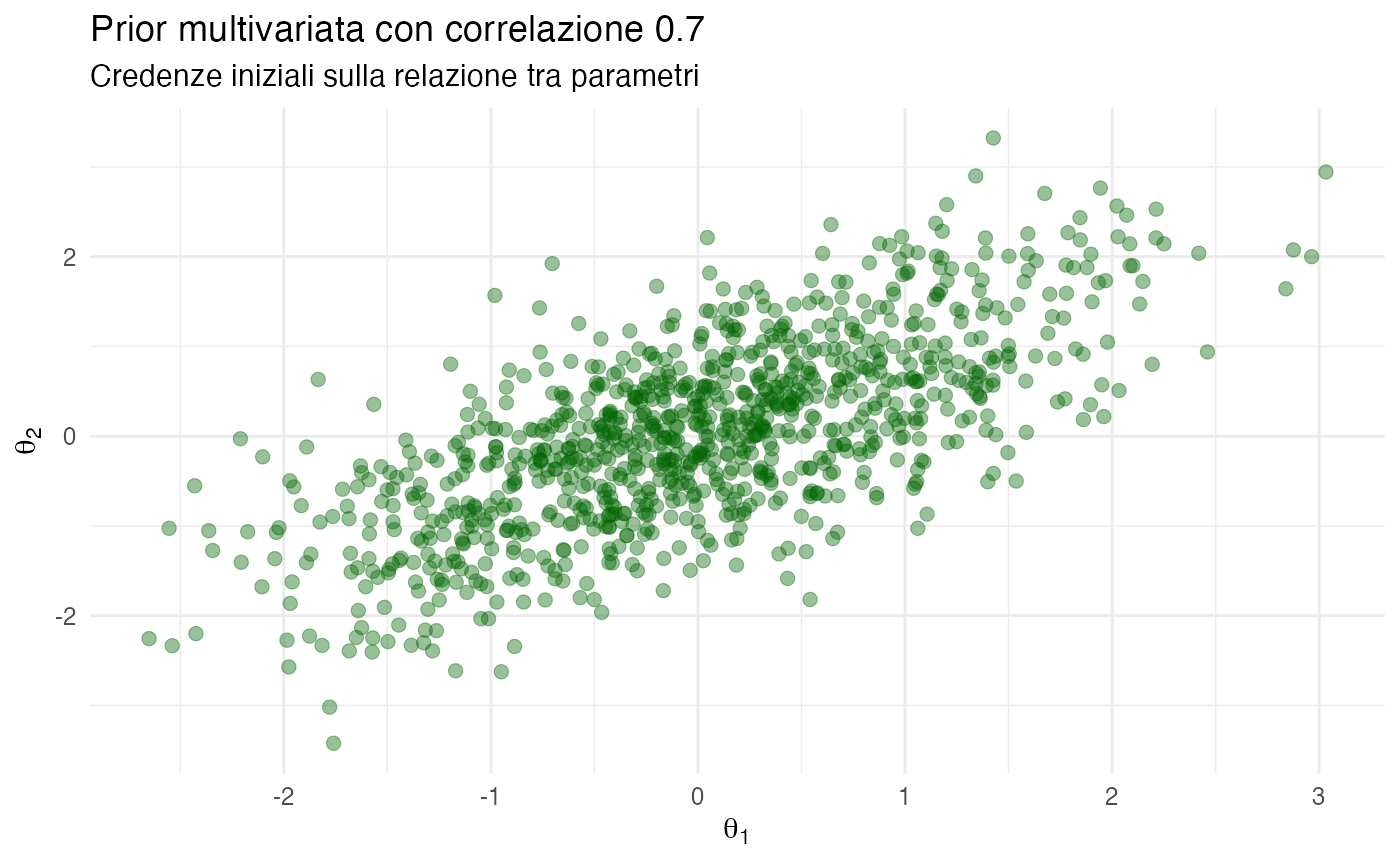
\includegraphics[width=0.85\linewidth,height=\textheight,keepaspectratio]{chapters/probability/10_cov_cor_files/figure-pdf/unnamed-chunk-10-1.png}
\end{center}

Specificando una correlazione positiva di 0.7 nella prior, stiamo
esprimendo la credenza che i due parametri tendano a variare insieme: se
uno è alto rispetto alla media, l'altro probabilmente lo è pure. Questa
informazione a priori influenzerà le inferenze a posteriori.

\subsection{Covarianza a posteriori}\label{covarianza-a-posteriori}

Dopo aver osservato i dati, la distribuzione a posteriori sui parametri
avrà una propria struttura di covarianza, che riflette l'aggiornamento
delle nostre credenze alla luce dell'evidenza. La covarianza a
posteriori può essere diversa da quella a priori: i dati possono
confermare, modificare persino ribaltare le nostre assunzioni iniziali
riguardo alla relazione tra i parametri.

\subsection{Covarianza predittiva}\label{covarianza-predittiva}

Quando utilizziamo il modello per fare previsioni su nuove osservazioni,
la covarianza predittiva caratterizza le nostre aspettative riguardo
alla relazione tra le variabili nei dati futuri. Tale quantità integra
l'incertezza sui parametri con la variabilità intrinseca del fenomeno.

\section*{Riflessioni conclusive}\label{riflessioni-conclusive-8}

\markright{Riflessioni conclusive}

La covarianza e la correlazione sono strumenti fondamentali per
quantificare le relazioni lineari tra variabili casuali. In questo
capitolo abbiamo visto come questi indici emergano naturalmente dalla
distribuzione congiunta e ne rappresentino una sintesi numerica.

Il percorso concettuale può essere riassunto in termini di livelli di
informazione, dal più completo al più sintetico. La
\textbf{distribuzione congiunta} \(p(x,y)\) o \(f(x,y)\) contiene tutte
le informazioni sulla relazione tra le variabili e consente di calcolare
qualsiasi quantità di interesse. La \textbf{covarianza}
\(\text{Cov}(X,Y)\) è un riassunto unidimensionale della co-variazione
lineare, utile per calcoli ma dipendente dalle unità di misura. La
\textbf{correlazione} \(\rho(X,Y)\) è la versione standardizzata della
covarianza, con scala interpretabile \([-1, 1]\) che facilita i
confronti.

Il punto chiave è che la covarianza e la correlazione catturano solo
l'aspetto lineare della relazione. Per una comprensione completa delle
dipendenze tra le variabili, incluse eventuali relazioni non lineari,
multimodali o complesse, è necessario tornare alla distribuzione
congiunta sottostante. La visualizzazione dei dati rimane una pratica
imprescindibile.

Nel proseguimento del manuale, incontreremo spesso distribuzioni
multivariate, in particolare la distribuzione normale multivariata, in
cui la matrice di covarianza \(\Sigma\) codifica completamente la
struttura di dipendenza lineare. La comprensione dei concetti sviluppati
in questo capitolo sarà essenziale per l'interpretazione di questi
modelli avanzati.

\begin{tcolorbox}[enhanced jigsaw, arc=.35mm, breakable, colbacktitle=quarto-callout-note-color!10!white, opacityback=0, toprule=.15mm, rightrule=.15mm, colback=white, opacitybacktitle=0.6, leftrule=.75mm, coltitle=black, bottomtitle=1mm, left=2mm, toptitle=1mm, title=\textcolor{quarto-callout-note-color}{\faInfo}\hspace{0.5em}{Informazioni sull'ambiente di sviluppo}, titlerule=0mm, bottomrule=.15mm, colframe=quarto-callout-note-color-frame]

\begin{Shaded}
\begin{Highlighting}[]
\FunctionTok{sessionInfo}\NormalTok{()}
\CommentTok{\#\textgreater{} R version 4.5.2 (2025{-}10{-}31)}
\CommentTok{\#\textgreater{} Platform: aarch64{-}apple{-}darwin20}
\CommentTok{\#\textgreater{} Running under: macOS Tahoe 26.1}
\CommentTok{\#\textgreater{} }
\CommentTok{\#\textgreater{} Matrix products: default}
\CommentTok{\#\textgreater{} BLAS:   /System/Library/Frameworks/Accelerate.framework/Versions/A/Frameworks/vecLib.framework/Versions/A/libBLAS.dylib }
\CommentTok{\#\textgreater{} LAPACK: /Library/Frameworks/R.framework/Versions/4.5{-}arm64/Resources/lib/libRlapack.dylib;  LAPACK version 3.12.1}
\CommentTok{\#\textgreater{} }
\CommentTok{\#\textgreater{} locale:}
\CommentTok{\#\textgreater{} [1] C.UTF{-}8/UTF{-}8/C.UTF{-}8/C/C.UTF{-}8/C.UTF{-}8}
\CommentTok{\#\textgreater{} }
\CommentTok{\#\textgreater{} time zone: Europe/Rome}
\CommentTok{\#\textgreater{} tzcode source: internal}
\CommentTok{\#\textgreater{} }
\CommentTok{\#\textgreater{} attached base packages:}
\CommentTok{\#\textgreater{} [1] stats     graphics  grDevices utils     datasets  methods   base     }
\CommentTok{\#\textgreater{} }
\CommentTok{\#\textgreater{} other attached packages:}
\CommentTok{\#\textgreater{}  [1] ggExtra\_0.11.0        viridis\_0.6.5         viridisLite\_0.4.2    }
\CommentTok{\#\textgreater{}  [4] MASS\_7.3{-}65           pillar\_1.11.1         tinytable\_0.15.1     }
\CommentTok{\#\textgreater{}  [7] patchwork\_1.3.2       ggdist\_3.3.3          tidybayes\_3.0.7      }
\CommentTok{\#\textgreater{} [10] bayesplot\_1.14.0      ggplot2\_4.0.1         reliabilitydiag\_0.2.1}
\CommentTok{\#\textgreater{} [13] priorsense\_1.2.0      posterior\_1.6.1       loo\_2.8.0            }
\CommentTok{\#\textgreater{} [16] rstan\_2.32.7          StanHeaders\_2.32.10   brms\_2.23.0          }
\CommentTok{\#\textgreater{} [19] Rcpp\_1.1.0            sessioninfo\_1.2.3     conflicted\_1.2.0     }
\CommentTok{\#\textgreater{} [22] janitor\_2.2.1         matrixStats\_1.5.0     modelr\_0.1.11        }
\CommentTok{\#\textgreater{} [25] tibble\_3.3.0          dplyr\_1.1.4           tidyr\_1.3.1          }
\CommentTok{\#\textgreater{} [28] rio\_1.2.4             here\_1.0.2           }
\CommentTok{\#\textgreater{} }
\CommentTok{\#\textgreater{} loaded via a namespace (and not attached):}
\CommentTok{\#\textgreater{}  [1] gridExtra\_2.3         inline\_0.3.21         sandwich\_3.1{-}1       }
\CommentTok{\#\textgreater{}  [4] rlang\_1.1.6           magrittr\_2.0.4        multcomp\_1.4{-}29      }
\CommentTok{\#\textgreater{}  [7] snakecase\_0.11.1      otel\_0.2.0            compiler\_4.5.2       }
\CommentTok{\#\textgreater{} [10] systemfonts\_1.3.1     vctrs\_0.6.5           stringr\_1.6.0        }
\CommentTok{\#\textgreater{} [13] pkgconfig\_2.0.3       arrayhelpers\_1.1{-}0    fastmap\_1.2.0        }
\CommentTok{\#\textgreater{} [16] backports\_1.5.0       labeling\_0.4.3        promises\_1.5.0       }
\CommentTok{\#\textgreater{} [19] rmarkdown\_2.30        ragg\_1.5.0            purrr\_1.2.0          }
\CommentTok{\#\textgreater{} [22] xfun\_0.54             cachem\_1.1.0          jsonlite\_2.0.0       }
\CommentTok{\#\textgreater{} [25] later\_1.4.4           broom\_1.0.10          parallel\_4.5.2       }
\CommentTok{\#\textgreater{} [28] R6\_2.6.1              stringi\_1.8.7         RColorBrewer\_1.1{-}3   }
\CommentTok{\#\textgreater{} [31] lubridate\_1.9.4       estimability\_1.5.1    knitr\_1.50           }
\CommentTok{\#\textgreater{} [34] zoo\_1.8{-}14            httpuv\_1.6.16         Matrix\_1.7{-}4         }
\CommentTok{\#\textgreater{} [37] splines\_4.5.2         timechange\_0.3.0      tidyselect\_1.2.1     }
\CommentTok{\#\textgreater{} [40] abind\_1.4{-}8           yaml\_2.3.10           codetools\_0.2{-}20     }
\CommentTok{\#\textgreater{} [43] miniUI\_0.1.2          curl\_7.0.0            pkgbuild\_1.4.8       }
\CommentTok{\#\textgreater{} [46] lattice\_0.22{-}7        shiny\_1.11.1          withr\_3.0.2          }
\CommentTok{\#\textgreater{} [49] bridgesampling\_1.2{-}1  S7\_0.2.1              coda\_0.19{-}4.1        }
\CommentTok{\#\textgreater{} [52] evaluate\_1.0.5        survival\_3.8{-}3        isoband\_0.2.7        }
\CommentTok{\#\textgreater{} [55] RcppParallel\_5.1.11{-}1 tensorA\_0.36.2.1      checkmate\_2.3.3      }
\CommentTok{\#\textgreater{} [58] stats4\_4.5.2          distributional\_0.5.0  generics\_0.1.4       }
\CommentTok{\#\textgreater{} [61] rprojroot\_2.1.1       rstantools\_2.5.0      scales\_1.4.0         }
\CommentTok{\#\textgreater{} [64] xtable\_1.8{-}4          glue\_1.8.0            emmeans\_2.0.0        }
\CommentTok{\#\textgreater{} [67] tools\_4.5.2           mvtnorm\_1.3{-}3         grid\_4.5.2           }
\CommentTok{\#\textgreater{} [70] QuickJSR\_1.8.1        colorspace\_2.1{-}2      nlme\_3.1{-}168         }
\CommentTok{\#\textgreater{} [73] cli\_3.6.5             textshaping\_1.0.4     svUnit\_1.0.8         }
\CommentTok{\#\textgreater{} [76] Brobdingnag\_1.2{-}9     V8\_8.0.1              gtable\_0.3.6         }
\CommentTok{\#\textgreater{} [79] digest\_0.6.39         TH.data\_1.1{-}5         farver\_2.1.2         }
\CommentTok{\#\textgreater{} [82] memoise\_2.0.1         htmltools\_0.5.8.1     lifecycle\_1.0.4      }
\CommentTok{\#\textgreater{} [85] mime\_0.13}
\end{Highlighting}
\end{Shaded}

\end{tcolorbox}

\section*{Bibliografia}\label{bibliografia-6}

\markright{Bibliografia}

\chapter{Introduzione alle distribuzioni di
probabilità}\label{sec-prob-intro-distr}

\section*{Introduzione}\label{introduzione-10}

\markright{Introduzione}

Nei capitoli precedenti abbiamo costruito il framework per ragionare in
modo coerente in condizioni di incertezza. Abbiamo visto che,
nell'interpretazione bayesiana, la probabilità rappresenta il grado di
credenza razionale che attribuiamo a proposizioni sul mondo e che gli
assiomi di Kolmogorov fungono da vincoli di coerenza logica per evitare
contraddizioni nelle nostre assegnazioni. Abbiamo poi esplorato le
distribuzioni congiunte come strumento per rappresentare le credenze sui
sistemi multivariati e la covarianza e la correlazione come sintesi
numeriche della struttura di dipendenza.

Ora, ci troviamo di fronte a una domanda pratica: come possiamo
rappresentare concretamente le nostre credenze? Se devo esprimere
l'incertezza sulla proporzione di pazienti che risponderanno a un
trattamento o sul tempo di reazione medio in un compito cognitivo, ho
bisogno di strumenti che traducano l'idea astratta di ``distribuzione di
probabilità'' in forme matematiche specifiche e maneggevoli.

Le famiglie parametriche di distribuzioni, come quelle normale,
binomiale, beta e gamma, forniscono un vocabolario matematico per
esprimere l'incertezza. Ogni famiglia ha una ``personalità'' distintiva
che la rende adatta a rappresentare determinati tipi di credenze.
Conoscere questo vocabolario significa poter comunicare le proprie
assunzioni in modo preciso, ragionare formalmente sulle conseguenze di
tali assunzioni e aggiornare le proprie credenze quando si osservano
nuovi dati.

\begin{tcolorbox}[enhanced jigsaw, arc=.35mm, breakable, colbacktitle=quarto-callout-tip-color!10!white, opacityback=0, toprule=.15mm, rightrule=.15mm, colback=white, opacitybacktitle=0.6, leftrule=.75mm, coltitle=black, bottomtitle=1mm, left=2mm, toptitle=1mm, title=\textcolor{quarto-callout-tip-color}{\faLightbulb}\hspace{0.5em}{Prerequisiti}, titlerule=0mm, bottomrule=.15mm, colframe=quarto-callout-tip-color-frame]

\begin{itemize}
\tightlist
\item
  Chapter~\ref{sec-prob-axioms-coherence}: assiomi e coerenza delle
  credenze.
\item
  Chapter~\ref{sec-prob-cov-cor}: covarianza e correlazione.
\end{itemize}

\end{tcolorbox}

\section{L'incertezza come condizione
epistemica}\label{lincertezza-come-condizione-epistemica}

\subsection{Perché abbiamo bisogno delle
distribuzioni}\label{perchuxe9-abbiamo-bisogno-delle-distribuzioni}

Nel ragionamento scientifico, ci troviamo costantemente in uno stato di
conoscenza incompleta. Non conosciamo con certezza il valore esatto di
un parametro di interesse, che si tratti della prevalenza di un
disturbo, dell'efficacia di un intervento o della correlazione tra due
costrutti psicologici. Tale incertezza non è un difetto del metodo
scientifico, ma una sua caratteristica costitutiva: la scienza procede
proprio attraverso la riduzione progressiva dell'incertezza, non
attraverso la sua eliminazione totale.

L'approccio bayesiano riconosce esplicitamente questa condizione e la
pone al centro del ragionamento inferenziale. L'incertezza non viene
nascosta dietro stime puntuali o decisioni binarie (significativo/non
significativo), ma viene rappresentata, quantificata e comunicata
attraverso distribuzioni di probabilità.

In questa prospettiva, una distribuzione di probabilità non descrive
principalmente ``come sono distribuiti i dati nel mondo'', ma piuttosto
``quali valori riteniamo più o meno plausibili, in base al nostro
attuale stato di conoscenza''. Questa distinzione è sottile, ma
fondamentale: la distribuzione è uno strumento epistemico, non una
proprietà ontologica del fenomeno.

\subsection{Dalla credenza puntuale alla credenza
distribuita}\label{dalla-credenza-puntuale-alla-credenza-distribuita}

Immaginiamo di voler esprimere le nostre credenze sulla proporzione di
studenti universitari che soffrono di ansia clinicamente rilevante,
\(\theta\). Un approccio ingenuo potrebbe suggerire di indicare un
valore singolo: ``Credo che sia il 25\%''. Tuttavia, questa risposta è
epistemicamente inadeguata, in quanto non riesce a catturare
l'incertezza che accompagna la nostra credenza.

Una rappresentazione più onesta riconosce che non siamo ugualmente
sicuri di tutti i possibili valori di \(\theta\). Forse riteniamo molto
plausibili i valori compresi tra 0.20 e 0.30, moderatamente plausibili
quelli compresi tra 0.15 e 0.35 e quasi incredibili i valori inferiori a
0.05 o superiori a 0.50. Una distribuzione di probabilità su \(\theta\)
cattura esattamente questa struttura di credenze graduata.

La distribuzione Beta, che incontreremo nei prossimi capitoli, è
particolarmente adatta a rappresentare le credenze sulle proporzioni.
Una distribuzione Beta(5, 15), per esempio, esprime la credenza che il
valore di \(\theta\) sia probabilmente intorno a 0.25, con maggiore
incertezza verso i valori più alti rispetto a quelli più bassi. I
parametri della distribuzione --- in questo caso 5 e 15 --- codificano
in modo compatto l'intera struttura delle nostre credenze.

\section{Il duplice ruolo delle distribuzioni nell'inferenza
bayesiana}\label{il-duplice-ruolo-delle-distribuzioni-nellinferenza-bayesiana}

Nell'approccio bayesiano, le distribuzioni di probabilità svolgono due
funzioni distinte ma complementari, corrispondenti ai due lati del
teorema di Bayes.

\subsection{Distribuzioni come rappresentazione dell'incertezza sui
parametri}\label{distribuzioni-come-rappresentazione-dellincertezza-sui-parametri}

Il primo ruolo, quello più distintamente bayesiano, riguarda la
rappresentazione dell'incertezza sui parametri del modello. Prima di
osservare i dati, esprimiamo le nostre credenze iniziali attraverso una
\textbf{distribuzione a priori} (\emph{prior}). Questa distribuzione
codifica ciò che sappiamo, o crediamo di sapere, sul parametro prima di
raccogliere nuove evidenze, come informazioni dalla letteratura
scientifica, vincoli teorici, esperienza clinica o l'ammissione di
grande incertezza.

Dopo aver osservato i dati, aggiorniamo le nostre credenze ottenendo una
\textbf{distribuzione a posteriori}. Questa nuova distribuzione
rappresenta il nostro stato di conoscenza aggiornato e integra le
informazioni pregresse con l'evidenza empirica appena raccolta. La forma
della distribuzione a posteriori --- la sua posizione, dispersione,
eventuale asimmetria o multimodalità --- comunica in modo completo
quanto abbiamo appreso e quanta incertezza residua permane.

In questo modo, la distribuzione risponde alla domanda: ``Quanto dovrei
credere in ciascun possibile valore del parametro?''.

\subsection{Distribuzioni come modelli
generativi}\label{distribuzioni-come-modelli-generativi}

Il secondo ruolo riguarda la specificazione di come i dati potrebbero
essere stati generati, in base a un determinato valore del parametro.
Questa è la \textbf{funzione di verosimiglianza}, che risponde alla
domanda: ``Se il parametro assumesse questo valore particolare, quanto
sarebbero plausibili i dati che ho osservato?''

Quando si assume che i tempi di reazione seguano una distribuzione gamma
o che le risposte a un item dicotomico seguano una distribuzione di
Bernoulli, si stanno facendo ipotesi sulla struttura generativa dei
dati. Queste assunzioni determinano la forma della funzione di
verosimiglianza e, di conseguenza, influenzano il modo in cui i dati
aggiornano le nostre credenze.

La scelta del modello generativo riflette le nostre ipotesi sulla natura
del fenomeno: i tempi di reazione sono sempre positivi e tipicamente
asimmetrici (il che suggerisce distribuzioni come la gamma o la
log-normale); i conteggi di eventi rari presentano una struttura
particolare (il che suggerisce la distribuzione di Poisson); le
proporzioni sono vincolate tra 0 e 1 (il che suggerisce la distribuzione
beta per la prior e la binomiale per la verosimiglianza).

\subsection{L'interazione tra i due
ruoli}\label{linterazione-tra-i-due-ruoli}

Il teorema di Bayes collega formalmente questi due ruoli:

\[
\underbrace{p(\theta \mid \text{dati})}_{\text{posterior}} \propto \underbrace{p(\text{dati} \mid \theta)}_{\text{verosimiglianza}} \times \underbrace{p(\theta)}_{\text{prior}}
\]

La distribuzione a posteriori emerge dall'interazione tra le nostre
credenze iniziali (prior) e l'evidenza contenuta nei dati
(verosimiglianza). Entrambe le componenti sono espresse tramite
distribuzioni di probabilità, rendendo le famiglie parametriche
strumenti indispensabili per l'inferenza bayesiana.

\section{Le famiglie parametriche come
vocabolario}\label{le-famiglie-parametriche-come-vocabolario}

\subsection{Cosa significa ``famiglia
parametrica''}\label{cosa-significa-famiglia-parametrica}

Una famiglia parametrica di distribuzioni è un insieme di distribuzioni
che condividono la stessa forma funzionale ma differiscono per i valori
di uno o più parametri. La famiglia normale, ad esempio, include
infinite distribuzioni, tutte a forma di campana simmetrica, che
differiscono per la loro posizione (parametro \(\mu\)) e dispersione
(parametro \(\sigma\)).

Specificare una famiglia parametrica significa fare un'assunzione sulla
\emph{forma} della distribuzione, mentre specificare i valori dei
parametri significa collocarsi in un punto particolare all'interno di
tale famiglia. Nell'inferenza bayesiana, di solito si fissa la famiglia
(ad esempio, ``credo che la distribuzione sia normale'') e si lascia che
siano i dati a informare i valori dei parametri.

\subsection{Il vocabolario delle
forme}\label{il-vocabolario-delle-forme}

Ogni famiglia parametrica presenta caratteristiche distintive che la
rendono adatta a rappresentare determinati tipi di credenze o fenomeni.

Le \textbf{distribuzioni discrete} assegnano probabilità a valori
distinti e contabili. La distribuzione di Bernoulli modella eventi
binari (successo/fallimento); la distribuzione binomiale conta i
successi in una serie di prove; la distribuzione di Poisson modella il
conteggio degli eventi rari in intervalli di tempo o spazio.

Le \textbf{distribuzioni continue} assegnano una densità di probabilità
a intervalli di valori su scale numeriche continue. La distribuzione
normale, con la sua caratteristica forma a campana simmetrica, emerge
naturalmente quando un fenomeno è influenzato da molti fattori
indipendenti di piccolo effetto. La distribuzione gamma modella le
quantità positive con possibile asimmetria, come i tempi di attesa o le
durate. La distribuzione beta, definita sull'intervallo {[}0,1{]}, è
ideale per rappresentare proporzioni o probabilità.

\subsection{Parsimonia e
flessibilità}\label{parsimonia-e-flessibilituxe0}

Le famiglie parametriche rappresentano un compromesso tra parsimonia e
flessibilità. Con pochi parametri, tipicamente da uno a tre, possono
rappresentare un'ampia gamma di forme distribuzionali. La distribuzione
normale richiede solo due parametri, \(\mu\) e \(\sigma,\) per essere
completamente specificata; la distribuzione beta richiede due parametri,
\(\alpha\) e \(\beta,\) per rappresentare credenze su proporzioni che
possono essere simmetriche, asimmetriche a destra o a sinistra,
concentrate o disperse.

Questa parsimonia è epistemicamente virtuosa: ci costringe a rendere
esplicite le nostre assunzioni fondamentali senza perderci in dettagli
non supportati dall'evidenza. Al tempo stesso, la varietà delle famiglie
disponibili garantisce una flessibilità sufficiente per adattarsi alle
caratteristiche dei diversi fenomeni psicologici.

\section{Applicazione: la variabilità nei fenomeni
psicologici}\label{applicazione-la-variabilituxe0-nei-fenomeni-psicologici}

\subsection{Perché la variabilità richiede un trattamento
distribuzionale}\label{perchuxe9-la-variabilituxe0-richiede-un-trattamento-distribuzionale}

Le considerazioni epistemiche sviluppate finora trovano un'applicazione
particolarmente importante nella ricerca psicologica, dove la
variabilità tra individui, nel tempo e tra contesti è la norma piuttosto
che l'eccezione.

Un recente articolo di Segal et al.
(\citeproc{ref-segal2025embracing}{2025}) sui disturbi mentali illustra
efficacemente questo punto. L'autore osserva che i limiti nella
comprensione dell'eziologia dei disturbi psichiatrici derivano dalla
sottovalutazione sistematica della variabilità. Storicamente, la ricerca
ha confrontato gruppi di pazienti con gruppi di controllo, identificando
differenze nelle medie come tratti distintivi. Questo approccio, sebbene
abbia prodotto risultati utili, trascura un dato fondamentale: i
disturbi psichiatrici sono caratterizzati da un'estrema eterogeneità che
i confronti tra medie non possono cogliere. I numeri sono eloquenti. Per
il disturbo da stress post-traumatico, ad esempio, esistono oltre
636,000 possibili combinazioni di sintomi che soddisfano i criteri
diagnostici. Per quanto riguarda la depressione maggiore, le
configurazioni sintomatologiche compatibili con la diagnosi superano le
16,000. Meno del 50\% dei pazienti depressi presenta la stessa
configurazione di sintomi.

\subsection{Oltre le medie di gruppo}\label{oltre-le-medie-di-gruppo}

Quando confrontiamo le medie di due gruppi e riscontriamo una differenza
``statisticamente significativa'', stiamo facendo un'affermazione sulla
popolazione nel suo complesso. Tale affermazione può essere
epistemicamente inadeguata se la variabilità all'interno dei gruppi è
molto maggiore della differenza tra i gruppi stessi, se le distribuzioni
si sovrappongono sostanzialmente o se esistono sottogruppi eterogenei
mascherati dalla media complessiva.

In questi casi, la media diventa un riassunto fuorviante. Rappresentare
l'intera distribuzione, con la sua forma, dispersione e, eventualmente,
multimodalità, fornisce un quadro molto più fedele del nostro stato di
conoscenza.

L'approccio bayesiano, che fa un uso sistematico delle distribuzioni di
probabilità, è naturalmente attrezzato per affrontare questa
complessità. Non ci limitiamo a stimare il valore più probabile di un
parametro, ma otteniamo un'intera distribuzione posteriore che
quantifica l'incertezza. I modelli gerarchici permettono di stimare
simultaneamente i parametri della popolazione e i parametri individuali,
catturando la variabilità tra i soggetti. I modelli di miscela, infine,
permettono di identificare sottogruppi eterogenei all'interno di
campioni apparentemente omogenei.

\subsection{La variabilità come
informazione}\label{la-variabilituxe0-come-informazione}

In questa prospettiva, la variabilità non è ``rumore'' da eliminare
statisticamente, ma informazione da modellare e comprendere. Le
distribuzioni di probabilità diventano strumenti per rappresentare
esplicitamente questa variabilità: una distribuzione con alta varianza
comunica qualcosa di diverso rispetto a una distribuzione con bassa
varianza e, in contesti diversi, entrambe possono essere epistemicamente
appropriate.

Come osserva Segal et al. (\citeproc{ref-segal2025embracing}{2025}),
solo integrando sistematicamente la variabilità nell'analisi empirica è
possibile sviluppare modelli predittivi robusti e interventi mirati alla
diversità individuale. Le famiglie parametriche di distribuzioni
forniscono il linguaggio formale per realizzare questa integrazione.

\section{Verso i capitoli successivi}\label{verso-i-capitoli-successivi}

Nei prossimi capitoli esploreremo le principali famiglie di
distribuzioni utilizzate nella ricerca psicologica.

Il Chapter~\ref{sec-prob-discr-distr} tratterà le \textbf{distribuzioni
discrete}: la distribuzione di Bernoulli per gli eventi binari singoli,
la distribuzione binomiale per i conteggi dei successi e la
distribuzione di Poisson per gli eventi rari. Queste distribuzioni sono
fondamentali per modellare le risposte categoriali, le frequenze e i
conteggi.

Il Chapter~\ref{sec-prob-cont-distr} affronterà le \textbf{distribuzioni
continue}: la normale per i fenomeni influenzati da molti fattori, la
gamma e la log-normale per le quantità positive asimmetriche, la beta
per le proporzioni e le probabilità e la t di Student per le situazioni
in cui c'è incertezza sulla varianza.

Per ciascuna di queste famiglie, esamineremo la forma della
distribuzione e il significato dei parametri, le proprietà matematiche
rilevanti, le situazioni in cui è appropriato utilizzarla e il suo ruolo
nell'inferenza bayesiana come prior, verosimiglianza o posterior.

\subsection{Una nota epistemologica}\label{una-nota-epistemologica}

È importante ricordare che nessuna distribuzione è ``vera'' in senso
assoluto. Come sottolineava George Box, ``tutti i modelli sono
sbagliati, ma alcuni sono utili''. La scelta di una famiglia parametrica
è sempre un'approssimazione pragmatica: cerchiamo distribuzioni che
catturino gli aspetti salienti del fenomeno con sufficiente accuratezza
e parsimonia, non la verità assoluta.

Nel framework bayesiano, questa consapevolezza è incorporata nel metodo
stesso. Possiamo confrontare i modelli alternativi tramite il fattore di
Bayes, combinare i modelli tramite il model averaging e verificare la
bontà dell'adattamento tramite i posterior predictive checks.
L'incertezza nella scelta del modello diventa così quantificabile e
gestibile.

\section*{Riflessioni conclusive}\label{riflessioni-conclusive-9}

\markright{Riflessioni conclusive}

Nel framework bayesiano, le distribuzioni di probabilità sono strumenti
per rappresentare e comunicare l'incertezza. Ogni distribuzione fornisce
una risposta formale alla domanda: ``Quanto dovrei credere in ciascun
possibile valore?''.

Le famiglie parametriche offrono un vocabolario ricco e flessibile per
esprimere diversi tipi di credenze. La scelta della famiglia riflette le
nostre assunzioni sulla natura del fenomeno, mentre i valori dei
parametri codificano il nostro stato di conoscenza specifico.
Nell'inferenza bayesiana, questo vocabolario viene utilizzato per
specificare sia le credenze a priori sui parametri, sia le ipotesi su
come i dati vengono generati.

L'applicazione alla ricerca psicologica rivela l'importanza di questo
approccio. La variabilità caratteristica dei fenomeni psicologici, che
si manifesta tra individui, nel tempo e tra contesti diversi, richiede
strumenti che vadano oltre i semplici confronti tra medie. Le
distribuzioni di probabilità permettono di rappresentare l'intera
struttura della variabilità trasformandola da ``rumore'' da ignorare a
informazione da modellare.

Nei capitoli seguenti, costruiremo progressivamente questo vocabolario,
esplorando le famiglie di distribuzioni che si sono rivelate più utili
per la ricerca psicologica. L'obiettivo non è memorizzare formule, ma
sviluppare un'intuizione su quale tipo di distribuzione sia più
appropriato in determinate circostanze e su come utilizzare queste
distribuzioni per ragionare in modo rigoroso in situazioni di
incertezza.

\section*{Bibliografia}\label{bibliografia-7}

\markright{Bibliografia}

\chapter{Distribuzioni di variabili casuali
discrete}\label{sec-prob-discr-distr}

\begin{tcolorbox}[enhanced jigsaw, arc=.35mm, breakable, colbacktitle=quarto-callout-tip-color!10!white, opacityback=0, toprule=.15mm, rightrule=.15mm, colback=white, opacitybacktitle=0.6, leftrule=.75mm, coltitle=black, bottomtitle=1mm, left=2mm, toptitle=1mm, title=\textcolor{quarto-callout-tip-color}{\faLightbulb}\hspace{0.5em}{Prerequisiti}, titlerule=0mm, bottomrule=.15mm, colframe=quarto-callout-tip-color-frame]

\begin{itemize}
\tightlist
\item
  Chapter~\ref{sec-prob-intro-distr}: introduzione alle distribuzioni di
  probabilità.
\end{itemize}

\end{tcolorbox}

\begin{tcolorbox}[enhanced jigsaw, arc=.35mm, breakable, colbacktitle=quarto-callout-caution-color!10!white, opacityback=0, toprule=.15mm, rightrule=.15mm, colback=white, opacitybacktitle=0.6, leftrule=.75mm, coltitle=black, bottomtitle=1mm, left=2mm, toptitle=1mm, title=\textcolor{quarto-callout-caution-color}{\faFire}\hspace{0.5em}{Preparazione del Notebook}, titlerule=0mm, bottomrule=.15mm, colframe=quarto-callout-caution-color-frame]

\begin{Shaded}
\begin{Highlighting}[]
\NormalTok{here}\SpecialCharTok{::}\FunctionTok{here}\NormalTok{(}\StringTok{"code"}\NormalTok{, }\StringTok{"\_common.R"}\NormalTok{) }\SpecialCharTok{|\textgreater{}} 
  \FunctionTok{source}\NormalTok{()}
\FunctionTok{library}\NormalTok{(reshape2)}
\FunctionTok{library}\NormalTok{(VGAM)}
\FunctionTok{library}\NormalTok{(extraDistr)}
\end{Highlighting}
\end{Shaded}

\end{tcolorbox}

\section*{Introduzione}\label{introduzione-11}

\markright{Introduzione}

Come discusso nel Chapter~\ref{sec-prob-intro-distr}, le distribuzioni
di probabilità sono strumenti epistemici che ci permettono di
rappresentare formalmente l'incertezza. In questo capitolo esploreremo
le \emph{distribuzioni discrete}, che modellano fenomeni con esiti
numerabili, come conteggi, scelte categoriali ed eventi binari.

Nell'inferenza bayesiana, le distribuzioni discrete svolgono tre ruoli
complementari. In qualità di \textbf{verosimiglianza}, modellano il modo
in cui i dati sono generati in funzione di un determinato valore del
parametro. Come \textbf{prior e posterior}, rappresentano le nostre
credenze sui parametri prima e dopo l'osservazione dei dati. Come
\textbf{distribuzioni predittive}, descrivono le nostre aspettative
riguardo a osservazioni future, integrando l'incertezza parametrica.

In questa prospettiva, i parametri delle distribuzioni, come \(p\) nella
distribuzione binomiale o \(\lambda\) nella distribuzione di Poisson,
non sono ``valori veri da scoprire'', ma quantità su cui abbiamo delle
credenze che aggiorniamo in modo coerente alla luce dei dati.

\section{Funzioni R per le
distribuzioni}\label{funzioni-r-per-le-distribuzioni}

Per ogni distribuzione, R fornisce quattro funzioni con prefissi
standardizzati:

\begin{Shaded}
\begin{Highlighting}[]
\CommentTok{\# Esempio con binomiale: n=10 prove, p=0.6 probabilità di successo}

\CommentTok{\# d = densità (massa di probabilità)}
\FunctionTok{dbinom}\NormalTok{(}\DecValTok{7}\NormalTok{, }\AttributeTok{size =} \DecValTok{10}\NormalTok{, }\AttributeTok{prob =} \FloatTok{0.6}\NormalTok{)  }\CommentTok{\# P(X = 7)}
\CommentTok{\#\textgreater{} [1] 0.215}

\CommentTok{\# p = probabilità cumulativa  }
\FunctionTok{pbinom}\NormalTok{(}\DecValTok{7}\NormalTok{, }\AttributeTok{size =} \DecValTok{10}\NormalTok{, }\AttributeTok{prob =} \FloatTok{0.6}\NormalTok{)  }\CommentTok{\# P(X ≤ 7)}
\CommentTok{\#\textgreater{} [1] 0.833}

\CommentTok{\# q = quantile}
\FunctionTok{qbinom}\NormalTok{(}\FloatTok{0.95}\NormalTok{, }\AttributeTok{size =} \DecValTok{10}\NormalTok{, }\AttributeTok{prob =} \FloatTok{0.6}\NormalTok{)  }\CommentTok{\# 95° percentile}
\CommentTok{\#\textgreater{} [1] 8}

\CommentTok{\# r = generazione casuale}
\FunctionTok{rbinom}\NormalTok{(}\DecValTok{5}\NormalTok{, }\AttributeTok{size =} \DecValTok{10}\NormalTok{, }\AttributeTok{prob =} \FloatTok{0.6}\NormalTok{)  }\CommentTok{\# 5 simulazioni}
\CommentTok{\#\textgreater{} [1] 6 5 6 6 4}
\end{Highlighting}
\end{Shaded}

Nell'inferenza bayesiana, la funzione \texttt{d} viene utilizzata per
calcolare la verosimiglianza, mentre la funzione \texttt{r} permette di
simulare dalla distribuzione predittiva.

\section{Distribuzione uniforme
discreta}\label{distribuzione-uniforme-discreta}

\subsection{Definizione e interpretazione
epistemica}\label{definizione-e-interpretazione-epistemica-1}

\begin{definition}[]\protect\hypertarget{def-uniform-discrete}{}\label{def-uniform-discrete}

Una variabile casuale \(X\) ha distribuzione uniforme su
\(\{1, \dots, N\}\) se ogni valore ha uguale probabilità:

\[
X \sim \text{Uniforme-Discreta}(N), \quad P(X = x) = \frac{1}{N} \text{ per } x \in \{1, \ldots, N\}.
\]

\textbf{Proprietà}: \(\mathbb{E}(X) = \frac{N+1}{2}\),
\(\mathbb{V}(X) = \frac{N^2-1}{12}\).

\end{definition}

\textbf{Interpretazione epistemica}: la distribuzione uniforme discreta
rappresenta il \emph{principio di indifferenza}, ovvero esprime la
massima ignoranza tra \(N\) alternative quando non abbiamo ragioni per
preferirne una rispetto alle altre.

\subsection{Ruolo nell'inferenza
bayesiana}\label{ruolo-nellinferenza-bayesiana}

La distribuzione uniforme discreta viene impiegata come \textbf{prior
non informativa} su insiemi finiti di ipotesi. Ad esempio, se dobbiamo
scegliere tra \(K\) modelli alternativi senza alcuna informazione
pregressa, possiamo assegnare a ciascuno di essi la probabilità
\(P(M_k) = 1/K\).

\subsection{Esempio: dado equo}\label{esempio-dado-equo}

\begin{Shaded}
\begin{Highlighting}[]
\CommentTok{\# Simulazione di 10000 lanci di dado}
\NormalTok{N }\OtherTok{\textless{}{-}} \DecValTok{6}
\FunctionTok{set.seed}\NormalTok{(}\DecValTok{42}\NormalTok{)}
\NormalTok{lanci }\OtherTok{\textless{}{-}} \FunctionTok{sample}\NormalTok{(}\DecValTok{1}\SpecialCharTok{:}\NormalTok{N, }\AttributeTok{size =} \DecValTok{10000}\NormalTok{, }\AttributeTok{replace =} \ConstantTok{TRUE}\NormalTok{)}

\FunctionTok{cat}\NormalTok{(}\StringTok{"Media teorica:"}\NormalTok{, (N}\SpecialCharTok{+}\DecValTok{1}\NormalTok{)}\SpecialCharTok{/}\DecValTok{2}\NormalTok{, }\StringTok{"| Empirica:"}\NormalTok{, }\FunctionTok{round}\NormalTok{(}\FunctionTok{mean}\NormalTok{(lanci), }\DecValTok{2}\NormalTok{), }\StringTok{"}\SpecialCharTok{\textbackslash{}n}\StringTok{"}\NormalTok{)}
\CommentTok{\#\textgreater{} Media teorica: 3.5 | Empirica: 3.46}
\FunctionTok{cat}\NormalTok{(}\StringTok{"Varianza teorica:"}\NormalTok{, }\FunctionTok{round}\NormalTok{((N}\SpecialCharTok{\^{}}\DecValTok{2{-}1}\NormalTok{)}\SpecialCharTok{/}\DecValTok{12}\NormalTok{, }\DecValTok{2}\NormalTok{), }\StringTok{"| Empirica:"}\NormalTok{, }\FunctionTok{round}\NormalTok{(}\FunctionTok{var}\NormalTok{(lanci), }\DecValTok{2}\NormalTok{))}
\CommentTok{\#\textgreater{} Varianza teorica: 2.92 | Empirica: 2.87}
\end{Highlighting}
\end{Shaded}

\section{Distribuzione di Bernoulli}\label{distribuzione-di-bernoulli}

\subsection{Definizione e interpretazione
epistemica}\label{definizione-e-interpretazione-epistemica-2}

\begin{definition}[]\protect\hypertarget{def-bernoulli}{}\label{def-bernoulli}

Una variabile casuale \(X\) segue una distribuzione di Bernoulli con
parametro \(p \in [0,1]\) se può assumere solo due valori: 1
(``successo'') con probabilità \(p\), e 0 (``insuccesso'') con
probabilità \(1-p\):

\[
X \sim \text{Bernoulli}(p), \quad P(X = x) = p^x (1-p)^{1-x}, \quad x \in \{0,1\}.
\]

\textbf{Proprietà}: \(\mathbb{E}(X) = p\), \(\mathbb{V}(X) = p(1-p)\).

\end{definition}

\textbf{Interpretazione epistemica}: il parametro \(p\) rappresenta il
grado di credenza nel verificarsi dell'evento ``successo''. La varianza
\(p(1-p)\) raggiunge il suo valore massimo quando \(p = 0,5\),
riflettendo il massimo livello di incertezza in una situazione di
completa indecisione tra i due possibili esiti.

\subsection{Ruolo nell'inferenza
bayesiana}\label{ruolo-nellinferenza-bayesiana-1}

La distribuzione di Bernoulli è fondamentale per modellare i
\textbf{dati binari}. Ogni singola osservazione binaria (sì/no,
presente/assente, corretto/errato) segue una distribuzione di Bernoulli.
La somma di \(n\) Bernoulli indipendenti con lo stesso parametro \(p\)
produce una distribuzione binomiale.

La \textbf{prior coniugata} per \(p\) è la distribuzione beta.

\subsection{Esempio: sensibilità di un
test}\label{esempio-sensibilituxe0-di-un-test}

\begin{Shaded}
\begin{Highlighting}[]
\CommentTok{\# Test diagnostico con sensibilità 0.85}
\NormalTok{p\_sens }\OtherTok{\textless{}{-}} \FloatTok{0.85}
\FunctionTok{set.seed}\NormalTok{(}\DecValTok{123}\NormalTok{)}
\NormalTok{risultati }\OtherTok{\textless{}{-}} \FunctionTok{rbinom}\NormalTok{(}\DecValTok{1000}\NormalTok{, }\AttributeTok{size =} \DecValTok{1}\NormalTok{, }\AttributeTok{prob =}\NormalTok{ p\_sens)}

\FunctionTok{cat}\NormalTok{(}\StringTok{"Proporzione campionaria di test positivi:"}\NormalTok{, }\FunctionTok{round}\NormalTok{(}\FunctionTok{mean}\NormalTok{(risultati), }\DecValTok{3}\NormalTok{), }\StringTok{"}\SpecialCharTok{\textbackslash{}n}\StringTok{"}\NormalTok{)}
\CommentTok{\#\textgreater{} Proporzione campionaria di test positivi: 0.853}
\FunctionTok{cat}\NormalTok{(}\StringTok{"Valore teorico:"}\NormalTok{, p\_sens)}
\CommentTok{\#\textgreater{} Valore teorico: 0.85}
\end{Highlighting}
\end{Shaded}

\section{Distribuzione binomiale}\label{distribuzione-binomiale}

\subsection{Definizione e interpretazione
epistemica}\label{definizione-e-interpretazione-epistemica-3}

\begin{definition}[]\protect\hypertarget{def-binomial}{}\label{def-binomial}

Una variabile casuale \(X\) che conta il numero di successi in \(n\)
prove indipendenti di Bernoulli, ciascuna con probabilità di successo
\(p\), segue una distribuzione binomiale:

\[
X \sim \text{Binomiale}(n, p), \quad P(X = k) = \binom{n}{k} p^k (1-p)^{n-k}, \quad k = 0, 1, \dots, n.
\]

\textbf{Proprietà}: \(\mathbb{E}(X) = np\), \(\mathbb{V}(X) = np(1-p)\).

\end{definition}

\textbf{Interpretazione epistemica}: la distribuzione binomiale modella
le nostre credenze sul numero di successi quando conosciamo il numero di
prove \(n\) e abbiamo delle credenze sul parametro \(p\). Il
coefficiente binomiale \(\binom{n}{k}\) indica il numero di modi in cui
\(k\) successi possono distribuirsi tra \(n\) prove.

\begin{tcolorbox}[enhanced jigsaw, arc=.35mm, breakable, colbacktitle=quarto-callout-note-color!10!white, opacityback=0, toprule=.15mm, rightrule=.15mm, colback=white, opacitybacktitle=0.6, leftrule=.75mm, coltitle=black, bottomtitle=1mm, left=2mm, toptitle=1mm, title=\textcolor{quarto-callout-note-color}{\faInfo}\hspace{0.5em}{Derivazione della formula}, titlerule=0mm, bottomrule=.15mm, colframe=quarto-callout-note-color-frame]

Consideriamo \(n\) prove indipendenti con probabilità \(p\) di successo.
La probabilità di ottenere esattamente \(k\) successi in una specifica
sequenza ordinata è data da \(p^k (1-p)^{n-k}\). Poiché ci interessano
tutte le possibili sequenze con \(k\) successi (indipendentemente
dall'ordine), moltiplichiamo per il numero di tali sequenze, dato dal
coefficiente binomiale \(\binom{n}{k}\).

\end{tcolorbox}

\subsection{Ruolo nell'inferenza
bayesiana}\label{ruolo-nellinferenza-bayesiana-2}

La distribuzione binomiale costituisce la \textbf{verosimiglianza
fondamentale} per dati binari aggregati. Quando osserviamo \(y\)
successi in \(n\) prove, la verosimiglianza per \(p\) è:

\[
L(p \mid y, n) \propto p^y (1-p)^{n-y}.
\]

\textbf{Coniugazione beta-binomiale}: se
\(p \sim \text{Beta}(\alpha, \beta)\), allora:

\[
p \mid y \sim \text{Beta}(\alpha + y, \beta + n - y).
\]

Questa proprietà consente di aggiornare le credenze su \(p\) in modo
analitico: i parametri della posterior si ottengono semplicemente
sommando i conteggi osservati (ossia i successi e gli insuccessi) agli
pseudo-conteggi della prior (ossia \(\alpha - 1\) e \(\beta - 1\)).

\subsection{Esempio: aggiornamento
bayesiano}\label{esempio-aggiornamento-bayesiano}

\begin{Shaded}
\begin{Highlighting}[]
\CommentTok{\# Dati osservati: 23 successi su 30 prove}
\NormalTok{n }\OtherTok{\textless{}{-}} \DecValTok{30}
\NormalTok{y }\OtherTok{\textless{}{-}} \DecValTok{23}

\CommentTok{\# Prior: Beta(2, 2) {-} moderatamente informativa, centrata su 0.5}
\NormalTok{alpha\_prior }\OtherTok{\textless{}{-}} \DecValTok{2}
\NormalTok{beta\_prior }\OtherTok{\textless{}{-}} \DecValTok{2}

\CommentTok{\# Posterior: Beta(25, 9)}
\NormalTok{alpha\_post }\OtherTok{\textless{}{-}}\NormalTok{ alpha\_prior }\SpecialCharTok{+}\NormalTok{ y}
\NormalTok{beta\_post }\OtherTok{\textless{}{-}}\NormalTok{ beta\_prior }\SpecialCharTok{+}\NormalTok{ (n }\SpecialCharTok{{-}}\NormalTok{ y)}

\CommentTok{\# Visualizzazione}
\NormalTok{p\_seq }\OtherTok{\textless{}{-}} \FunctionTok{seq}\NormalTok{(}\DecValTok{0}\NormalTok{, }\DecValTok{1}\NormalTok{, }\AttributeTok{length.out =} \DecValTok{1000}\NormalTok{)}

\NormalTok{df }\OtherTok{\textless{}{-}} \FunctionTok{data.frame}\NormalTok{(}
  \AttributeTok{p =} \FunctionTok{rep}\NormalTok{(p\_seq, }\DecValTok{2}\NormalTok{),}
  \AttributeTok{densita =} \FunctionTok{c}\NormalTok{(}\FunctionTok{dbeta}\NormalTok{(p\_seq, alpha\_prior, beta\_prior), }
              \FunctionTok{dbeta}\NormalTok{(p\_seq, alpha\_post, beta\_post)),}
  \AttributeTok{tipo =} \FunctionTok{rep}\NormalTok{(}\FunctionTok{c}\NormalTok{(}\StringTok{"Prior Beta(2,2)"}\NormalTok{, }\StringTok{"Posterior Beta(25,9)"}\NormalTok{), }\AttributeTok{each =} \FunctionTok{length}\NormalTok{(p\_seq))}
\NormalTok{)}

\FunctionTok{ggplot}\NormalTok{(df, }\FunctionTok{aes}\NormalTok{(}\AttributeTok{x =}\NormalTok{ p, }\AttributeTok{y =}\NormalTok{ densita, }\AttributeTok{color =}\NormalTok{ tipo)) }\SpecialCharTok{+}
  \FunctionTok{geom\_line}\NormalTok{(}\AttributeTok{linewidth =} \FloatTok{1.2}\NormalTok{) }\SpecialCharTok{+}
  \FunctionTok{labs}\NormalTok{(}
    \AttributeTok{title =} \StringTok{"Aggiornamento Bayesiano: Beta{-}Binomiale"}\NormalTok{,}
    \AttributeTok{subtitle =} \StringTok{"23 successi su 30 prove"}\NormalTok{,}
    \AttributeTok{x =} \StringTok{"p"}\NormalTok{, }\AttributeTok{y =} \StringTok{"Densità"}
\NormalTok{  ) }\SpecialCharTok{+}
  \FunctionTok{theme\_minimal}\NormalTok{()}
\end{Highlighting}
\end{Shaded}

\begin{center}
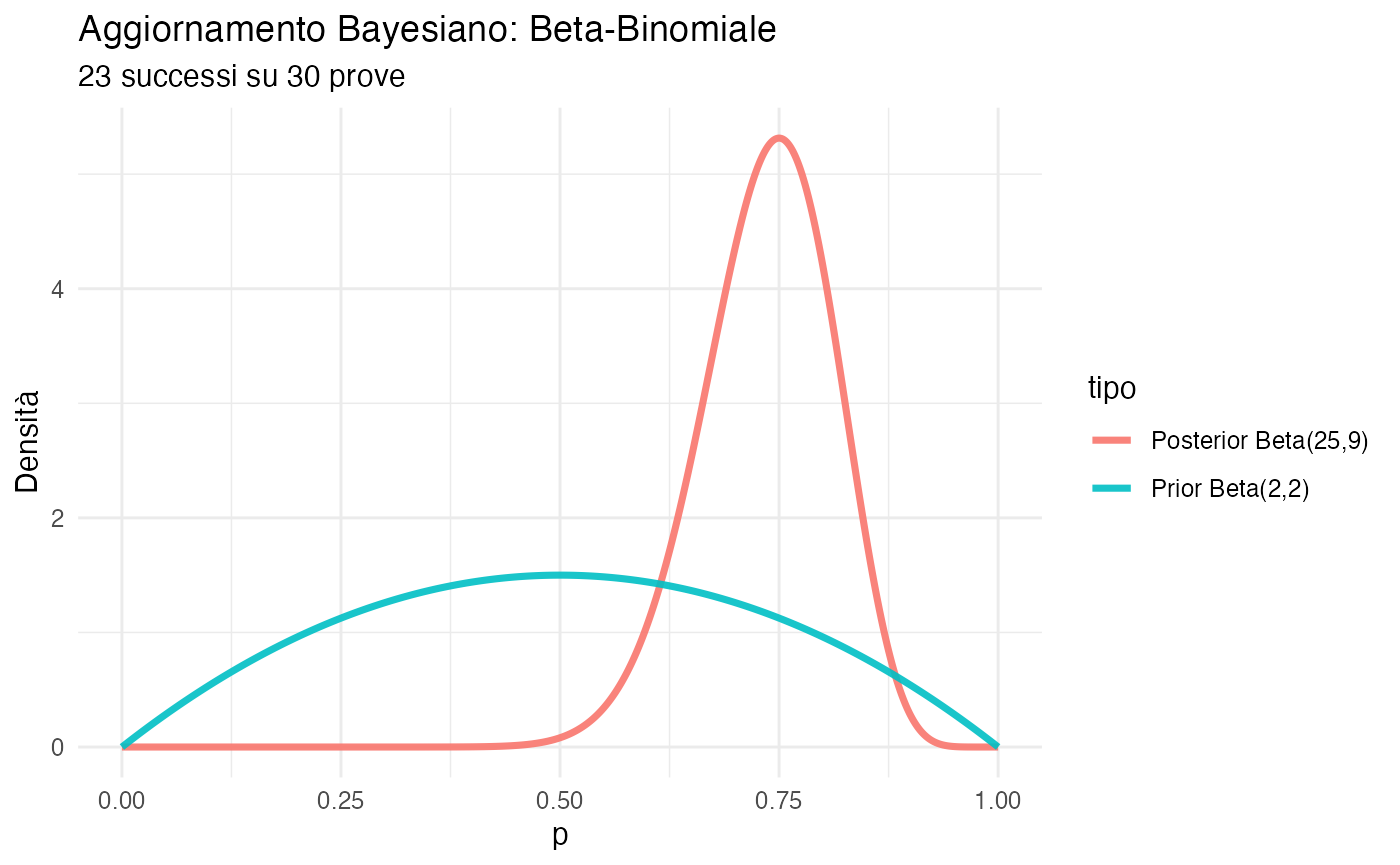
\includegraphics[width=0.85\linewidth,height=\textheight,keepaspectratio]{chapters/probability/12_discr_rv_distr_files/figure-pdf/unnamed-chunk-5-1.png}
\end{center}

\begin{Shaded}
\begin{Highlighting}[]

\FunctionTok{cat}\NormalTok{(}\StringTok{"Media prior:"}\NormalTok{, }\FunctionTok{round}\NormalTok{(alpha\_prior}\SpecialCharTok{/}\NormalTok{(alpha\_prior }\SpecialCharTok{+}\NormalTok{ beta\_prior), }\DecValTok{3}\NormalTok{), }\StringTok{"}\SpecialCharTok{\textbackslash{}n}\StringTok{"}\NormalTok{)}
\CommentTok{\#\textgreater{} Media prior: 0.5}
\FunctionTok{cat}\NormalTok{(}\StringTok{"Media posterior:"}\NormalTok{, }\FunctionTok{round}\NormalTok{(alpha\_post}\SpecialCharTok{/}\NormalTok{(alpha\_post }\SpecialCharTok{+}\NormalTok{ beta\_post), }\DecValTok{3}\NormalTok{), }\StringTok{"}\SpecialCharTok{\textbackslash{}n}\StringTok{"}\NormalTok{)}
\CommentTok{\#\textgreater{} Media posterior: 0.735}
\end{Highlighting}
\end{Shaded}

La posterior si concentra attorno a \(p \approx 0.74\), mostrando una
riduzione significativa dell'incertezza rispetto alla prior. Ciò
riflette l'aggiornamento coerente delle credenze alla luce dei 23
successi osservati.

\section{Distribuzione di Poisson}\label{distribuzione-di-poisson}

\subsection{Definizione e interpretazione
epistemica}\label{definizione-e-interpretazione-epistemica-4}

\begin{definition}[]\protect\hypertarget{def-poisson}{}\label{def-poisson}

Una variabile casuale \(Y\) segue una distribuzione di Poisson con
parametro \(\lambda > 0\) se modella il conteggio di eventi in un
intervallo di tempo o spazio:

\[
Y \sim \text{Poisson}(\lambda), \quad P(Y = y) = \frac{\lambda^y e^{-\lambda}}{y!}, \quad y = 0, 1, 2, \ldots
\]

\textbf{Proprietà caratteristica}:
\(\mathbb{E}(Y) = \mathbb{V}(Y) = \lambda\) (equidispersione).

\end{definition}

\textbf{Interpretazione epistemica}: il parametro \(\lambda\)
rappresenta il tasso atteso di occorrenza degli eventi nell'intervallo
considerato. L'equidispersione (uguaglianza di media e varianza) è
un'assunzione forte: nei dati psicologici, infatti, si osserva spesso la
\emph{sovradispersione} (varianza maggiore della media), che richiede
modelli alternativi come la distribuzione binomiale negativa.

\subsection{Ruolo nell'inferenza
bayesiana}\label{ruolo-nellinferenza-bayesiana-3}

\textbf{Coniugazione gamma-Poisson}: se
\(\lambda \sim \text{Gamma}(\alpha, \beta)\), dopo aver osservato
\(y_1, \ldots, y_n\) conteggi indipendenti, si ha:

\[
\lambda \mid \mathbf{y} \sim \text{Gamma}\left(\alpha + \sum_{i=1}^n y_i, \beta + n\right).
\]

Questa coniugazione permette di aggiornare analiticamente le credenze
sul tasso \(\lambda\).

\subsection{Esempio: analisi bayesiana di
conteggi}\label{esempio-analisi-bayesiana-di-conteggi}

Consideriamo il famoso dataset di von Bortkiewicz sui decessi causati da
calci di cavallo nell'esercito prussiano.

\begin{Shaded}
\begin{Highlighting}[]
\CommentTok{\# Dati storici}
\NormalTok{decessi }\OtherTok{\textless{}{-}} \DecValTok{0}\SpecialCharTok{:}\DecValTok{4}
\NormalTok{freq\_oss }\OtherTok{\textless{}{-}} \FunctionTok{c}\NormalTok{(}\DecValTok{109}\NormalTok{, }\DecValTok{65}\NormalTok{, }\DecValTok{22}\NormalTok{, }\DecValTok{3}\NormalTok{, }\DecValTok{1}\NormalTok{)}
\NormalTok{n\_tot }\OtherTok{\textless{}{-}} \FunctionTok{sum}\NormalTok{(freq\_oss)}

\CommentTok{\# Stima del tasso}
\NormalTok{lambda\_mle }\OtherTok{\textless{}{-}} \FunctionTok{sum}\NormalTok{(decessi }\SpecialCharTok{*}\NormalTok{ freq\_oss) }\SpecialCharTok{/}\NormalTok{ n\_tot}

\CommentTok{\# Confronto osservato vs teorico}
\FunctionTok{data.frame}\NormalTok{(}
  \AttributeTok{Decessi =}\NormalTok{ decessi,}
  \AttributeTok{Freq\_osservata =} \FunctionTok{round}\NormalTok{(freq\_oss }\SpecialCharTok{/}\NormalTok{ n\_tot, }\DecValTok{4}\NormalTok{),}
  \AttributeTok{Prob\_Poisson =} \FunctionTok{round}\NormalTok{(}\FunctionTok{dpois}\NormalTok{(decessi, }\AttributeTok{lambda =}\NormalTok{ lambda\_mle), }\DecValTok{4}\NormalTok{)}
\NormalTok{)}
\CommentTok{\#\textgreater{}   Decessi Freq\_osservata Prob\_Poisson}
\CommentTok{\#\textgreater{} 1       0          0.545       0.5434}
\CommentTok{\#\textgreater{} 2       1          0.325       0.3314}
\CommentTok{\#\textgreater{} 3       2          0.110       0.1011}
\CommentTok{\#\textgreater{} 4       3          0.015       0.0206}
\CommentTok{\#\textgreater{} 5       4          0.005       0.0031}
\end{Highlighting}
\end{Shaded}

\textbf{Analisi bayesiana}:

\begin{Shaded}
\begin{Highlighting}[]
\CommentTok{\# Prior debolmente informativa: Gamma(0.5, 1)}
\NormalTok{alpha\_prior }\OtherTok{\textless{}{-}} \FloatTok{0.5}
\NormalTok{beta\_prior }\OtherTok{\textless{}{-}} \DecValTok{1}

\CommentTok{\# Totale eventi e osservazioni}
\NormalTok{y\_tot }\OtherTok{\textless{}{-}} \FunctionTok{sum}\NormalTok{(decessi }\SpecialCharTok{*}\NormalTok{ freq\_oss)}

\CommentTok{\# Posterior: Gamma(alpha + y\_tot, beta + n\_tot)}
\NormalTok{alpha\_post }\OtherTok{\textless{}{-}}\NormalTok{ alpha\_prior }\SpecialCharTok{+}\NormalTok{ y\_tot}
\NormalTok{beta\_post }\OtherTok{\textless{}{-}}\NormalTok{ beta\_prior }\SpecialCharTok{+}\NormalTok{ n\_tot}

\CommentTok{\# Stime}
\NormalTok{lambda\_post }\OtherTok{\textless{}{-}}\NormalTok{ alpha\_post }\SpecialCharTok{/}\NormalTok{ beta\_post}
\NormalTok{IC\_95 }\OtherTok{\textless{}{-}} \FunctionTok{qgamma}\NormalTok{(}\FunctionTok{c}\NormalTok{(}\FloatTok{0.025}\NormalTok{, }\FloatTok{0.975}\NormalTok{), alpha\_post, beta\_post)}

\FunctionTok{cat}\NormalTok{(}\StringTok{"Media posterior di λ:"}\NormalTok{, }\FunctionTok{round}\NormalTok{(lambda\_post, }\DecValTok{3}\NormalTok{), }\StringTok{"}\SpecialCharTok{\textbackslash{}n}\StringTok{"}\NormalTok{)}
\CommentTok{\#\textgreater{} Media posterior di λ: 0.609}
\FunctionTok{cat}\NormalTok{(}\StringTok{"IC 95\%: ["}\NormalTok{, }\FunctionTok{round}\NormalTok{(IC\_95[}\DecValTok{1}\NormalTok{], }\DecValTok{3}\NormalTok{), }\StringTok{", "}\NormalTok{, }\FunctionTok{round}\NormalTok{(IC\_95[}\DecValTok{2}\NormalTok{], }\DecValTok{3}\NormalTok{), }\StringTok{"]}\SpecialCharTok{\textbackslash{}n}\StringTok{"}\NormalTok{, }\AttributeTok{sep =} \StringTok{""}\NormalTok{)}
\CommentTok{\#\textgreater{} IC 95\%: [0.506, 0.722]}
\end{Highlighting}
\end{Shaded}

L'ottima corrispondenza tra frequenze osservate e probabilità teoriche
conferma che il processo generativo è coerente con l'ipotesi di eventi
rari e indipendenti.

\section{Distribuzione
beta-binomiale}\label{distribuzione-beta-binomiale}

\subsection{Definizione e motivazione}\label{definizione-e-motivazione}

\begin{definition}[]\protect\hypertarget{def-beta-binomial}{}\label{def-beta-binomial}

La distribuzione beta-binomiale emerge quando il parametro \(p\) di una
distribuzione binomiale è esso stesso incerto e modellato con una
distribuzione beta:

\[
p \sim \text{Beta}(\alpha, \beta), \quad Y \mid p \sim \text{Binomiale}(n, p).
\]

Marginalizzando rispetto a \(p\), otteniamo:

\[
Y \sim \text{Beta-Binomiale}(n, \alpha, \beta), \quad P(Y = y) = \binom{n}{y} \frac{B(y + \alpha, n - y + \beta)}{B(\alpha, \beta)}.
\]

\end{definition}

\textbf{Interpretazione epistemica}: la distribuzione beta-binomiale è
la \textbf{distribuzione predittiva bayesiana} per il numero di successi
quando si ha incertezza sul parametro \(p\). Incorpora due fonti di
variabilità: quella campionaria (data \(p\), quanti successi?) e quella
epistemica (quale valore di \(p\)?).

\subsection{Differenza fondamentale dalla
binomiale}\label{differenza-fondamentale-dalla-binomiale}

\begin{longtable}[]{@{}lll@{}}
\toprule\noalign{}
Aspetto & Binomiale & Beta-binomiale \\
\midrule\noalign{}
\endhead
\bottomrule\noalign{}
\endlastfoot
Parametro \(p\) & Fisso e noto & Incerto (distribuzione beta) \\
Fonti di variabilità & Solo campionaria & Campionaria + epistemica \\
Varianza & \(np(1-p)\) & Maggiore (sovradispersione) \\
\end{longtable}

\subsection{Ruolo nell'inferenza
bayesiana}\label{ruolo-nellinferenza-bayesiana-4}

La distribuzione beta-binomiale è utile in tre contesti:

\begin{enumerate}
\def\labelenumi{\arabic{enumi}.}
\item
  \textbf{Distribuzione predittiva}: prima di osservare nuovi dati,
  rappresenta le nostre aspettative sul numero di successi integrando
  l'incertezza su \(p\).
\item
  \textbf{Modellazione della sovradispersione}: quando i dati presentano
  una varianza maggiore rispetto a quella prevista dalla distribuzione
  binomiale, la distribuzione beta-binomiale offre un modello più
  flessibile.
\item
  \textbf{Modelli gerarchici}: quando ogni unità ha il proprio parametro
  \(p_i\) proveniente da una distribuzione comune beta.
\end{enumerate}

\subsection{Esempio: confronto
predittivo}\label{esempio-confronto-predittivo}

\begin{Shaded}
\begin{Highlighting}[]
\CommentTok{\# Prior per p: Beta(5, 5)}
\NormalTok{n\_new }\OtherTok{\textless{}{-}} \DecValTok{10}
\NormalTok{alpha }\OtherTok{\textless{}{-}} \DecValTok{5}
\NormalTok{beta }\OtherTok{\textless{}{-}} \DecValTok{5}

\FunctionTok{set.seed}\NormalTok{(}\DecValTok{42}\NormalTok{)}
\CommentTok{\# Beta{-}binomiale: incorpora incertezza su p}
\NormalTok{y\_bb }\OtherTok{\textless{}{-}} \FunctionTok{rbetabinom}\NormalTok{(}\DecValTok{10000}\NormalTok{, }\AttributeTok{size =}\NormalTok{ n\_new, }\AttributeTok{prob =}\NormalTok{ alpha}\SpecialCharTok{/}\NormalTok{(alpha}\SpecialCharTok{+}\NormalTok{beta), }\AttributeTok{rho =} \DecValTok{1}\SpecialCharTok{/}\NormalTok{(alpha}\SpecialCharTok{+}\NormalTok{beta}\SpecialCharTok{+}\DecValTok{1}\NormalTok{))}

\CommentTok{\# Binomiale: p fissato alla media della prior}
\NormalTok{y\_bin }\OtherTok{\textless{}{-}} \FunctionTok{rbinom}\NormalTok{(}\DecValTok{10000}\NormalTok{, }\AttributeTok{size =}\NormalTok{ n\_new, }\AttributeTok{prob =}\NormalTok{ alpha}\SpecialCharTok{/}\NormalTok{(alpha}\SpecialCharTok{+}\NormalTok{beta))}

\FunctionTok{cat}\NormalTok{(}\StringTok{"Beta{-}Binomiale {-} Media:"}\NormalTok{, }\FunctionTok{round}\NormalTok{(}\FunctionTok{mean}\NormalTok{(y\_bb), }\DecValTok{3}\NormalTok{), }
    \StringTok{"| Varianza:"}\NormalTok{, }\FunctionTok{round}\NormalTok{(}\FunctionTok{var}\NormalTok{(y\_bb), }\DecValTok{3}\NormalTok{), }\StringTok{"}\SpecialCharTok{\textbackslash{}n}\StringTok{"}\NormalTok{)}
\CommentTok{\#\textgreater{} Beta{-}Binomiale {-} Media: 4.97 | Varianza: 4.56}
\FunctionTok{cat}\NormalTok{(}\StringTok{"Binomiale(p=0.5) {-} Media:"}\NormalTok{, }\FunctionTok{round}\NormalTok{(}\FunctionTok{mean}\NormalTok{(y\_bin), }\DecValTok{3}\NormalTok{), }
    \StringTok{"| Varianza:"}\NormalTok{, }\FunctionTok{round}\NormalTok{(}\FunctionTok{var}\NormalTok{(y\_bin), }\DecValTok{3}\NormalTok{), }\StringTok{"}\SpecialCharTok{\textbackslash{}n}\StringTok{"}\NormalTok{)}
\CommentTok{\#\textgreater{} Binomiale(p=0.5) {-} Media: 5 | Varianza: 2.55}
\end{Highlighting}
\end{Shaded}

La distribuzione beta-binomiale presenta una varianza maggiore perché
integra l'incertezza su \(p\). Questa è la previsione bayesiana coerente
quando il parametro non è noto con certezza.

\begin{Shaded}
\begin{Highlighting}[]
\CommentTok{\# Visualizzazione}
\NormalTok{df }\OtherTok{\textless{}{-}} \FunctionTok{data.frame}\NormalTok{(}
  \AttributeTok{y =} \FunctionTok{c}\NormalTok{(y\_bb, y\_bin),}
  \AttributeTok{tipo =} \FunctionTok{rep}\NormalTok{(}\FunctionTok{c}\NormalTok{(}\StringTok{"Beta{-}Binomiale"}\NormalTok{, }\StringTok{"Binomiale"}\NormalTok{), }\AttributeTok{each =} \DecValTok{10000}\NormalTok{)}
\NormalTok{)}

\FunctionTok{ggplot}\NormalTok{(df, }\FunctionTok{aes}\NormalTok{(}\AttributeTok{x =}\NormalTok{ y, }\AttributeTok{fill =}\NormalTok{ tipo)) }\SpecialCharTok{+}
  \FunctionTok{geom\_histogram}\NormalTok{(}\AttributeTok{position =} \StringTok{"dodge"}\NormalTok{, }\AttributeTok{bins =} \DecValTok{11}\NormalTok{, }\AttributeTok{alpha =} \FloatTok{0.7}\NormalTok{) }\SpecialCharTok{+}
  \FunctionTok{labs}\NormalTok{(}
    \AttributeTok{title =} \StringTok{"Confronto: Beta{-}Binomiale vs Binomiale"}\NormalTok{,}
    \AttributeTok{subtitle =} \StringTok{"La beta{-}binomiale ha code più pesanti (sovradispersione)"}\NormalTok{,}
    \AttributeTok{x =} \StringTok{"Numero di successi"}\NormalTok{, }\AttributeTok{y =} \StringTok{"Frequenza"}
\NormalTok{  ) }\SpecialCharTok{+}
  \FunctionTok{theme\_minimal}\NormalTok{()}
\end{Highlighting}
\end{Shaded}

\begin{center}
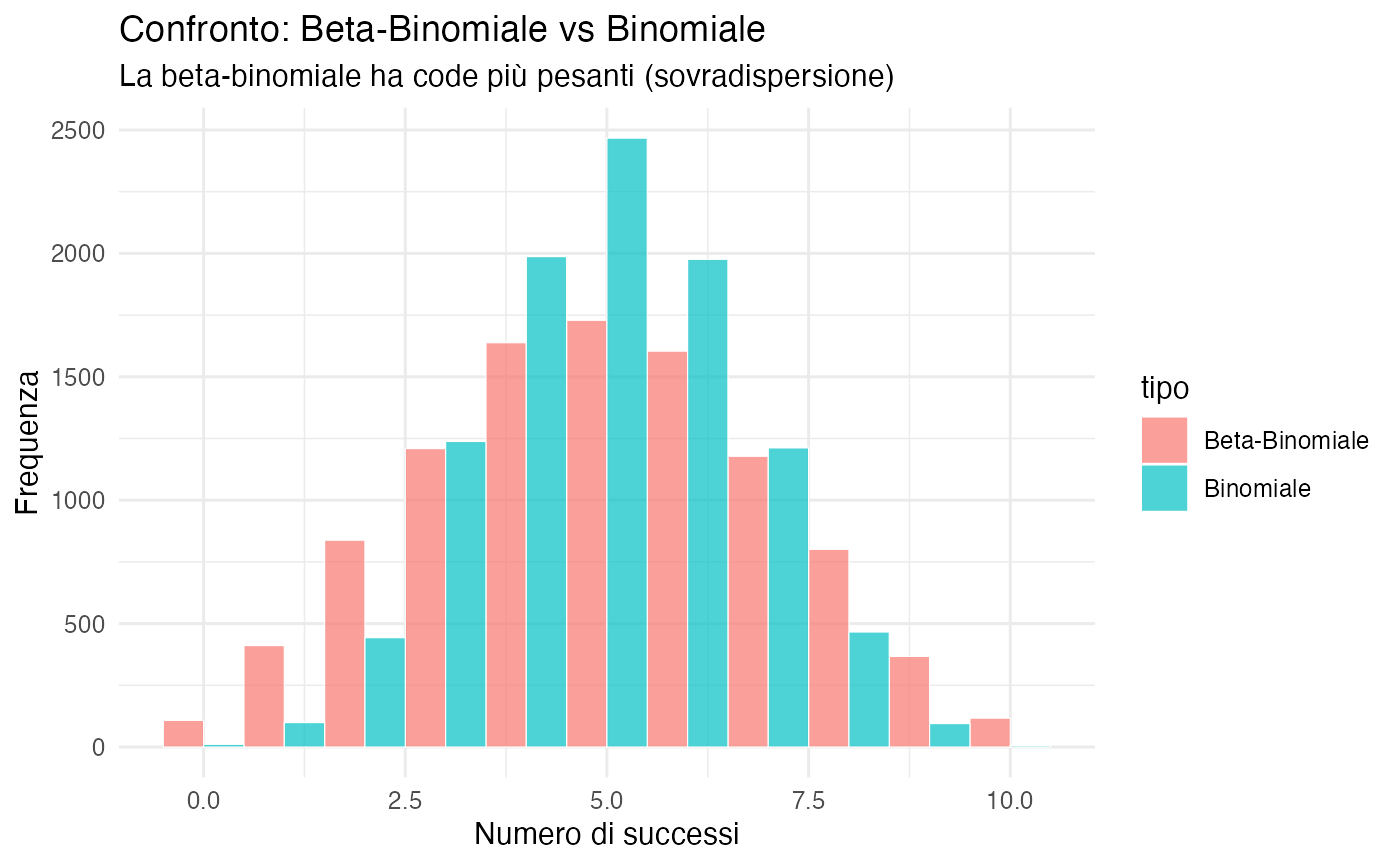
\includegraphics[width=0.85\linewidth,height=\textheight,keepaspectratio]{chapters/probability/12_discr_rv_distr_files/figure-pdf/unnamed-chunk-9-1.png}
\end{center}

\section*{Riflessioni conclusive}\label{riflessioni-conclusive-10}

\markright{Riflessioni conclusive}

Le distribuzioni discrete esaminate in questo capitolo sono strumenti
epistemici per la rappresentazione e l'aggiornamento delle credenze
relative a fenomeni caratterizzati da esiti numerabili. Ciascuna
distribuzione incorpora specifiche assunzioni riguardanti il processo di
generazione dei dati: la distribuzione uniforme discreta formalizza uno
stato di massima ignoranza riguardo a un insieme finito di alternative;
la distribuzione di Bernoulli modella eventi binari elementari; la
distribuzione binomiale conta i successi in serie di prove indipendenti
a probabilità costante; la distribuzione di Poisson rappresenta il
verificarsi di eventi rari con un tasso costante; la distribuzione
beta-binomiale, infine, estende il modello binomiale incorporando
l'incertezza sul parametro sottostante.

In questa prospettiva, i parametri di tali distribuzioni non sono
semplici quantità fisse da stimare, ma entità probabilistiche su cui
formulare distribuzioni di credenza. L'eleganza formale del framework
bayesiano si manifesta pienamente attraverso le proprietà di
coniugazione: la relazione beta-binomiale consente aggiornamenti
analitici per il parametro \(p\), mentre la coniugazione gamma-Poisson
opera analogamente per il parametro \(\lambda\).

Il prossimo capitolo sarà dedicato all'esplorazione delle distribuzioni
continue, come la distribuzione beta, la distribuzione gamma, la
distribuzione normale e altre, che fungeranno da distribuzioni a priori
naturali per i parametri delle distribuzioni discrete presentate in
questo capitolo, completando così il vocabolario probabilistico
essenziale per l'inferenza bayesiana.

\section*{Esercizi}\label{esercizi-2}
\addcontentsline{toc}{section}{Esercizi}

\markright{Esercizi}

\begin{tcolorbox}[enhanced jigsaw, arc=.35mm, breakable, colbacktitle=quarto-callout-important-color!10!white, opacityback=0, toprule=.15mm, rightrule=.15mm, colback=white, opacitybacktitle=0.6, leftrule=.75mm, coltitle=black, bottomtitle=1mm, left=2mm, toptitle=1mm, title=\textcolor{quarto-callout-important-color}{\faExclamation}\hspace{0.5em}{Esercizi di base}, titlerule=0mm, bottomrule=.15mm, colframe=quarto-callout-important-color-frame]

Per ciascuna distribuzione (uniforme, Bernoulli, binomiale, Poisson):

\begin{enumerate}
\def\labelenumi{\arabic{enumi}.}
\tightlist
\item
  Scegli parametri appropriati e visualizza la funzione di massa.
\item
  Simula 1000 osservazioni e confronta media/varianza empirica con
  quella teorica.
\item
  Calcola \(P(X \leq x)\) per qualche valore significativo.
\end{enumerate}

\end{tcolorbox}

\begin{tcolorbox}[enhanced jigsaw, arc=.35mm, breakable, colbacktitle=quarto-callout-important-color!10!white, opacityback=0, toprule=.15mm, rightrule=.15mm, colback=white, opacitybacktitle=0.6, leftrule=.75mm, coltitle=black, bottomtitle=1mm, left=2mm, toptitle=1mm, title=\textcolor{quarto-callout-important-color}{\faExclamation}\hspace{0.5em}{Esercizi bayesiani}, titlerule=0mm, bottomrule=.15mm, colframe=quarto-callout-important-color-frame]

\begin{enumerate}
\def\labelenumi{\arabic{enumi}.}
\tightlist
\item
  \textbf{Binomiale}:

  \begin{itemize}
  \tightlist
  \item
    Scegli una prior Beta(2, 2).
  \item
    Simula 20 osservazioni binarie con \(p_{\text{true}} = 0.7\).
  \item
    Calcola la posterior e l'intervallo di credibilità al 95\%.
  \end{itemize}
\item
  \textbf{Poisson}:

  \begin{itemize}
  \tightlist
  \item
    Scegli una prior Gamma(2, 1).
  \item
    Simula 10 conteggi con \(\lambda_{\text{true}} = 3\).
  \item
    Calcola posterior e intervallo di credibilità 95\%.
  \end{itemize}
\item
  \textbf{Confronto predittivo}:

  \begin{itemize}
  \tightlist
  \item
    Simula da Binomiale(10, 0.6) e da Beta-Binomiale(10, 3, 2).
  \item
    Confronta le varianze.
  \item
    Quale distribuzione assegna più probabilità ai valori estremi (0 o
    10)?
  \end{itemize}
\end{enumerate}

\end{tcolorbox}

\begin{tcolorbox}[enhanced jigsaw, arc=.35mm, breakable, colbacktitle=quarto-callout-important-color!10!white, opacityback=0, toprule=.15mm, rightrule=.15mm, colback=white, opacitybacktitle=0.6, leftrule=.75mm, coltitle=black, bottomtitle=1mm, left=2mm, toptitle=1mm, title=\textcolor{quarto-callout-important-color}{\faExclamation}\hspace{0.5em}{Progetto: Apprendimento sequenziale}, titlerule=0mm, bottomrule=.15mm, colframe=quarto-callout-important-color-frame]

Scrivi uno script R che:

\begin{enumerate}
\def\labelenumi{\arabic{enumi}.}
\tightlist
\item
  Inizia con una prior Beta(1, 1) su \(p\).
\item
  Simula osservazioni binarie sequenziali con \(p_{\text{true}} = 0.7\).
\item
  Aggiorna la posterior dopo ogni osservazione.
\item
  Visualizza l'evoluzione della posterior (es. ogni 5 osservazioni).
\item
  Mostra come l'incertezza diminuisce e la stima converge al valore
  vero.
\end{enumerate}

Questo illustra visivamente l'\emph{apprendimento bayesiano} come
processo di riduzione progressiva dell'incertezza.

\end{tcolorbox}

\begin{tcolorbox}[enhanced jigsaw, arc=.35mm, breakable, colbacktitle=quarto-callout-caution-color!10!white, opacityback=0, toprule=.15mm, rightrule=.15mm, colback=white, opacitybacktitle=0.6, leftrule=.75mm, coltitle=black, bottomtitle=1mm, left=2mm, toptitle=1mm, title=\textcolor{quarto-callout-caution-color}{\faFire}\hspace{0.5em}{Informazioni sull'ambiente di sviluppo}, titlerule=0mm, bottomrule=.15mm, colframe=quarto-callout-caution-color-frame]

\begin{Shaded}
\begin{Highlighting}[]
\FunctionTok{sessionInfo}\NormalTok{()}
\CommentTok{\#\textgreater{} R version 4.5.2 (2025{-}10{-}31)}
\CommentTok{\#\textgreater{} Platform: aarch64{-}apple{-}darwin20}
\CommentTok{\#\textgreater{} Running under: macOS Tahoe 26.1}
\CommentTok{\#\textgreater{} }
\CommentTok{\#\textgreater{} Matrix products: default}
\CommentTok{\#\textgreater{} BLAS:   /System/Library/Frameworks/Accelerate.framework/Versions/A/Frameworks/vecLib.framework/Versions/A/libBLAS.dylib }
\CommentTok{\#\textgreater{} LAPACK: /Library/Frameworks/R.framework/Versions/4.5{-}arm64/Resources/lib/libRlapack.dylib;  LAPACK version 3.12.1}
\CommentTok{\#\textgreater{} }
\CommentTok{\#\textgreater{} locale:}
\CommentTok{\#\textgreater{} [1] C.UTF{-}8/UTF{-}8/C.UTF{-}8/C/C.UTF{-}8/C.UTF{-}8}
\CommentTok{\#\textgreater{} }
\CommentTok{\#\textgreater{} time zone: Europe/Rome}
\CommentTok{\#\textgreater{} tzcode source: internal}
\CommentTok{\#\textgreater{} }
\CommentTok{\#\textgreater{} attached base packages:}
\CommentTok{\#\textgreater{} [1] splines   stats4    stats     graphics  grDevices utils     datasets }
\CommentTok{\#\textgreater{} [8] methods   base     }
\CommentTok{\#\textgreater{} }
\CommentTok{\#\textgreater{} other attached packages:}
\CommentTok{\#\textgreater{}  [1] extraDistr\_1.10.0     VGAM\_1.1{-}13           reshape2\_1.4.5       }
\CommentTok{\#\textgreater{}  [4] pillar\_1.11.1         tinytable\_0.15.1      patchwork\_1.3.2      }
\CommentTok{\#\textgreater{}  [7] ggdist\_3.3.3          tidybayes\_3.0.7       bayesplot\_1.14.0     }
\CommentTok{\#\textgreater{} [10] ggplot2\_4.0.1         reliabilitydiag\_0.2.1 priorsense\_1.2.0     }
\CommentTok{\#\textgreater{} [13] posterior\_1.6.1       loo\_2.8.0             rstan\_2.32.7         }
\CommentTok{\#\textgreater{} [16] StanHeaders\_2.32.10   brms\_2.23.0           Rcpp\_1.1.0           }
\CommentTok{\#\textgreater{} [19] sessioninfo\_1.2.3     conflicted\_1.2.0      janitor\_2.2.1        }
\CommentTok{\#\textgreater{} [22] matrixStats\_1.5.0     modelr\_0.1.11         tibble\_3.3.0         }
\CommentTok{\#\textgreater{} [25] dplyr\_1.1.4           tidyr\_1.3.1           rio\_1.2.4            }
\CommentTok{\#\textgreater{} [28] here\_1.0.2           }
\CommentTok{\#\textgreater{} }
\CommentTok{\#\textgreater{} loaded via a namespace (and not attached):}
\CommentTok{\#\textgreater{}  [1] gridExtra\_2.3         inline\_0.3.21         sandwich\_3.1{-}1       }
\CommentTok{\#\textgreater{}  [4] rlang\_1.1.6           magrittr\_2.0.4        multcomp\_1.4{-}29      }
\CommentTok{\#\textgreater{}  [7] snakecase\_0.11.1      compiler\_4.5.2        systemfonts\_1.3.1    }
\CommentTok{\#\textgreater{} [10] vctrs\_0.6.5           stringr\_1.6.0         pkgconfig\_2.0.3      }
\CommentTok{\#\textgreater{} [13] arrayhelpers\_1.1{-}0    fastmap\_1.2.0         backports\_1.5.0      }
\CommentTok{\#\textgreater{} [16] labeling\_0.4.3        rmarkdown\_2.30        ragg\_1.5.0           }
\CommentTok{\#\textgreater{} [19] purrr\_1.2.0           xfun\_0.54             cachem\_1.1.0         }
\CommentTok{\#\textgreater{} [22] jsonlite\_2.0.0        broom\_1.0.10          parallel\_4.5.2       }
\CommentTok{\#\textgreater{} [25] R6\_2.6.1              stringi\_1.8.7         RColorBrewer\_1.1{-}3   }
\CommentTok{\#\textgreater{} [28] lubridate\_1.9.4       estimability\_1.5.1    knitr\_1.50           }
\CommentTok{\#\textgreater{} [31] zoo\_1.8{-}14            Matrix\_1.7{-}4          timechange\_0.3.0     }
\CommentTok{\#\textgreater{} [34] tidyselect\_1.2.1      abind\_1.4{-}8           codetools\_0.2{-}20     }
\CommentTok{\#\textgreater{} [37] curl\_7.0.0            pkgbuild\_1.4.8        lattice\_0.22{-}7       }
\CommentTok{\#\textgreater{} [40] plyr\_1.8.9            withr\_3.0.2           bridgesampling\_1.2{-}1 }
\CommentTok{\#\textgreater{} [43] S7\_0.2.1              coda\_0.19{-}4.1         evaluate\_1.0.5       }
\CommentTok{\#\textgreater{} [46] survival\_3.8{-}3        RcppParallel\_5.1.11{-}1 tensorA\_0.36.2.1     }
\CommentTok{\#\textgreater{} [49] checkmate\_2.3.3       distributional\_0.5.0  generics\_0.1.4       }
\CommentTok{\#\textgreater{} [52] rprojroot\_2.1.1       rstantools\_2.5.0      scales\_1.4.0         }
\CommentTok{\#\textgreater{} [55] xtable\_1.8{-}4          glue\_1.8.0            emmeans\_2.0.0        }
\CommentTok{\#\textgreater{} [58] tools\_4.5.2           mvtnorm\_1.3{-}3         grid\_4.5.2           }
\CommentTok{\#\textgreater{} [61] QuickJSR\_1.8.1        colorspace\_2.1{-}2      nlme\_3.1{-}168         }
\CommentTok{\#\textgreater{} [64] cli\_3.6.5             textshaping\_1.0.4     svUnit\_1.0.8         }
\CommentTok{\#\textgreater{} [67] Brobdingnag\_1.2{-}9     V8\_8.0.1              gtable\_0.3.6         }
\CommentTok{\#\textgreater{} [70] digest\_0.6.39         TH.data\_1.1{-}5         farver\_2.1.2         }
\CommentTok{\#\textgreater{} [73] memoise\_2.0.1         htmltools\_0.5.8.1     lifecycle\_1.0.4      }
\CommentTok{\#\textgreater{} [76] MASS\_7.3{-}65}
\end{Highlighting}
\end{Shaded}

\end{tcolorbox}

\section*{Bibliografia}\label{bibliografia-8}
\addcontentsline{toc}{section}{Bibliografia}

\markright{Bibliografia}

\chapter{Distribuzioni di variabili casuali
continue}\label{sec-prob-cont-distr}

\begin{tcolorbox}[enhanced jigsaw, arc=.35mm, breakable, colbacktitle=quarto-callout-tip-color!10!white, opacityback=0, toprule=.15mm, rightrule=.15mm, colback=white, opacitybacktitle=0.6, leftrule=.75mm, coltitle=black, bottomtitle=1mm, left=2mm, toptitle=1mm, title=\textcolor{quarto-callout-tip-color}{\faLightbulb}\hspace{0.5em}{Prerequisiti}, titlerule=0mm, bottomrule=.15mm, colframe=quarto-callout-tip-color-frame]

\begin{itemize}
\tightlist
\item
  Chapter~\ref{sec-prob-intro-distr}: introduzione alle distribuzioni di
  probabilità.
\item
  Chapter~\ref{sec-prob-discr-distr}: distribuzioni discrete.
\end{itemize}

\end{tcolorbox}

\begin{tcolorbox}[enhanced jigsaw, arc=.35mm, breakable, colbacktitle=quarto-callout-caution-color!10!white, opacityback=0, toprule=.15mm, rightrule=.15mm, colback=white, opacitybacktitle=0.6, leftrule=.75mm, coltitle=black, bottomtitle=1mm, left=2mm, toptitle=1mm, title=\textcolor{quarto-callout-caution-color}{\faFire}\hspace{0.5em}{Preparazione del Notebook}, titlerule=0mm, bottomrule=.15mm, colframe=quarto-callout-caution-color-frame]

\begin{Shaded}
\begin{Highlighting}[]
\NormalTok{here}\SpecialCharTok{::}\FunctionTok{here}\NormalTok{(}\StringTok{"code"}\NormalTok{, }\StringTok{"\_common.R"}\NormalTok{) }\SpecialCharTok{|\textgreater{}} 
  \FunctionTok{source}\NormalTok{()}
\end{Highlighting}
\end{Shaded}

\end{tcolorbox}

\section*{Introduzione}\label{introduzione-12}

\markright{Introduzione}

Nel Chapter~\ref{sec-prob-discr-distr} abbiamo esplorato le
distribuzioni discrete come strumenti per rappresentare credenze su
fenomeni con esiti numerabili. In questo capitolo estendiamo il
framework alle \emph{distribuzioni continue}, che permettono di
esprimere credenze su quantità che assumono valori su scale numeriche
continue, come tempi, distanze, proporzioni, tassi e punteggi
psicometrici.

Le distribuzioni continue svolgono un ruolo complementare a quello delle
distribuzioni discrete nel framework bayesiano. Come
\textbf{verosimiglianza per i dati continui}, diverse famiglie di
distribuzioni catturano diversi tipi di processi generativi: la normale
per le misurazioni con errori simmetrici, l'esponenziale per i tempi di
attesa e la gamma per le variabili positive asimmetriche. Queste
distribuzioni esprimono e aggiornano le nostre credenze come prior e
posterior su parametri continui: la beta per probabilità
\(p \in (0,1)\), la gamma per tassi \(\lambda > 0\), la normale per
medie \(\mu \in \mathbb{R}\), e la Cauchy e la \(t\) di Student per
prior robusti con code pesanti.

Una caratteristica elegante dell'inferenza bayesiana è la
\textbf{dualità discreta-continua} espressa dalle famiglie coniugate: la
distribuzione binomiale si accompagna alla beta e la Poisson alla gamma.
Questa simmetria, introdotta nel capitolo precedente, trova ora il suo
completamento con l'esplorazione delle distribuzioni continue che
fungono da prior naturali per i parametri delle distribuzioni discrete.

\subsection*{Struttura del capitolo}\label{struttura-del-capitolo}

L'esplorazione seguirà una progressione che partirà da distribuzioni più
semplici per arrivare a quelle con ruoli più specifici nell'inferenza
bayesiana. Inizieremo con la distribuzione \textbf{uniforme}, che
rappresenta il caso di massima ignoranza su un intervallo. Poi passeremo
all'\textbf{esponenziale}, fondamentale per modellare tempi di attesa, e
alla \textbf{normale}, centrale per il Teorema del Limite Centrale.
Esamineremo poi la distribuzione \textbf{chi-quadrato} e la
\textbf{\(t\) di Student}, che derivano dalla distribuzione normale e
trovano applicazione come prior robusti. Concluderemo con le
distribuzioni di maggiore rilevanza bayesiana: la \textbf{beta} come
prior per le proporzioni, la \textbf{gamma} come prior per tassi e
varianze e la \textbf{Cauchy} come prior robusto a code pesanti.

Per ciascuna di queste distribuzioni, presenteremo la definizione
matematica, l'interpretazione epistemica dei parametri, il ruolo
nell'inferenza bayesiana e le applicazioni pratiche in R.

\section{Distribuzione uniforme
continua}\label{distribuzione-uniforme-continua}

\subsection{Definizione e interpretazione
epistemica}\label{definizione-e-interpretazione-epistemica-5}

La distribuzione uniforme continua rappresenta lo stato di massima
ignoranza all'interno di un intervallo definito: ogni valore
nell'intervallo è ritenuto ugualmente plausibile.

\begin{definition}[]\protect\hypertarget{def-uniform-cont}{}\label{def-uniform-cont}

Una variabile casuale \(X\) segue una distribuzione uniforme
sull'intervallo \([a, b]\) se la sua densità è costante:

\[
X \sim \text{Uniforme}(a, b), \quad f(x) = \frac{1}{b-a} \text{ per } x \in [a,b].
\]

\textbf{Proprietà}: \(\mathbb{E}(X) = \frac{a+b}{2}\),
\(\mathbb{V}(X) = \frac{(b-a)^2}{12}\).

\end{definition}

\textbf{Interpretazione epistemica}: la distribuzione uniforme codifica
il \emph{principio di indifferenza}, secondo il quale, quando non
abbiamo ragioni per preferire un valore rispetto a un altro all'interno
dell'intervallo, assegniamo la stessa probabilità a tutti i valori. Si
tratta dell'analogo continuo della distribuzione uniforme discreta.

\subsection{Ruolo nell'inferenza
bayesiana}\label{ruolo-nellinferenza-bayesiana-5}

La distribuzione uniforme viene impiegata come \textbf{prior non
informativa} quando si vuole esprimere l'assenza di conoscenze pregresse
su un parametro vincolato a un intervallo. Ad esempio,
\(\text{Uniforme}(0, 1)\) è equivalente alla distribuzione
\(\text{Beta}(1, 1)\) e rappresenta l'ignoranza riguardo a una
proporzione.

\textbf{Limiti come prior}: la distribuzione uniforme può essere
``troppo informativa'' in alcuni contesti, in quanto assegna una
credenza pari a zero ai valori esterni all'intervallo. Prior come la
Cauchy o la \(t\) di Student sono spesso preferite quando non si
desidera escludere completamente i valori estremi.

\subsection{Calcolo delle
probabilità}\label{calcolo-delle-probabilituxe0}

La probabilità che \(X\) assuma valori in un sottointervallo
\([c, d] \subseteq [a, b]\) è proporzionale alla lunghezza del
sottointervallo:

\[
P(c \leq X \leq d) = \frac{d - c}{b - a}.
\]

\begin{Shaded}
\begin{Highlighting}[]
\CommentTok{\# Esempio: probabilità che uno spinner (0{-}360°) si fermi tra 150° e 250°}
\NormalTok{prob }\OtherTok{\textless{}{-}}\NormalTok{ (}\DecValTok{250} \SpecialCharTok{{-}} \DecValTok{150}\NormalTok{) }\SpecialCharTok{/} \DecValTok{360}
\FunctionTok{cat}\NormalTok{(}\StringTok{"P(150 ≤ X ≤ 250) ="}\NormalTok{, }\FunctionTok{round}\NormalTok{(prob, }\DecValTok{4}\NormalTok{), }\StringTok{"}\SpecialCharTok{\textbackslash{}n}\StringTok{"}\NormalTok{)}
\CommentTok{\#\textgreater{} P(150 ≤ X ≤ 250) = 0.278}

\CommentTok{\# Equivalente con funzione R}
\FunctionTok{punif}\NormalTok{(}\DecValTok{250}\NormalTok{, }\AttributeTok{min =} \DecValTok{0}\NormalTok{, }\AttributeTok{max =} \DecValTok{360}\NormalTok{) }\SpecialCharTok{{-}} \FunctionTok{punif}\NormalTok{(}\DecValTok{150}\NormalTok{, }\AttributeTok{min =} \DecValTok{0}\NormalTok{, }\AttributeTok{max =} \DecValTok{360}\NormalTok{)}
\CommentTok{\#\textgreater{} [1] 0.278}
\end{Highlighting}
\end{Shaded}

\subsection{Visualizzazione}\label{visualizzazione}

\begin{Shaded}
\begin{Highlighting}[]
\NormalTok{x }\OtherTok{\textless{}{-}} \FunctionTok{seq}\NormalTok{(}\SpecialCharTok{{-}}\DecValTok{50}\NormalTok{, }\DecValTok{410}\NormalTok{, }\AttributeTok{length.out =} \DecValTok{500}\NormalTok{)}
\NormalTok{density\_uniform }\OtherTok{\textless{}{-}} \FunctionTok{dunif}\NormalTok{(x, }\AttributeTok{min =} \DecValTok{0}\NormalTok{, }\AttributeTok{max =} \DecValTok{360}\NormalTok{)}

\FunctionTok{ggplot}\NormalTok{(}\FunctionTok{data.frame}\NormalTok{(}\AttributeTok{x =}\NormalTok{ x, }\AttributeTok{y =}\NormalTok{ density\_uniform), }\FunctionTok{aes}\NormalTok{(}\AttributeTok{x =}\NormalTok{ x, }\AttributeTok{y =}\NormalTok{ y)) }\SpecialCharTok{+}
  \FunctionTok{geom\_line}\NormalTok{(}\AttributeTok{linewidth =} \FloatTok{1.2}\NormalTok{, }\AttributeTok{color =} \StringTok{"blue"}\NormalTok{) }\SpecialCharTok{+}
  \FunctionTok{geom\_area}\NormalTok{(}
    \AttributeTok{data =} \FunctionTok{subset}\NormalTok{(}\FunctionTok{data.frame}\NormalTok{(x, }\AttributeTok{y =}\NormalTok{ density\_uniform), x }\SpecialCharTok{\textgreater{}=} \DecValTok{150} \SpecialCharTok{\&}\NormalTok{ x }\SpecialCharTok{\textless{}=} \DecValTok{250}\NormalTok{),}
    \FunctionTok{aes}\NormalTok{(}\AttributeTok{x =}\NormalTok{ x, }\AttributeTok{y =}\NormalTok{ y), }
    \AttributeTok{fill =} \StringTok{"steelblue"}\NormalTok{, }\AttributeTok{alpha =} \FloatTok{0.5}
\NormalTok{  ) }\SpecialCharTok{+}
  \FunctionTok{labs}\NormalTok{(}
    \AttributeTok{title =} \StringTok{"Distribuzione Uniforme (0, 360)"}\NormalTok{,}
    \AttributeTok{subtitle =} \StringTok{"Area evidenziata: P(150 ≤ X ≤ 250)"}\NormalTok{,}
    \AttributeTok{x =} \StringTok{"x"}\NormalTok{, }\AttributeTok{y =} \StringTok{"Densità f(x)"}
\NormalTok{  ) }\SpecialCharTok{+}
  \FunctionTok{theme\_minimal}\NormalTok{()}
\end{Highlighting}
\end{Shaded}

\begin{center}
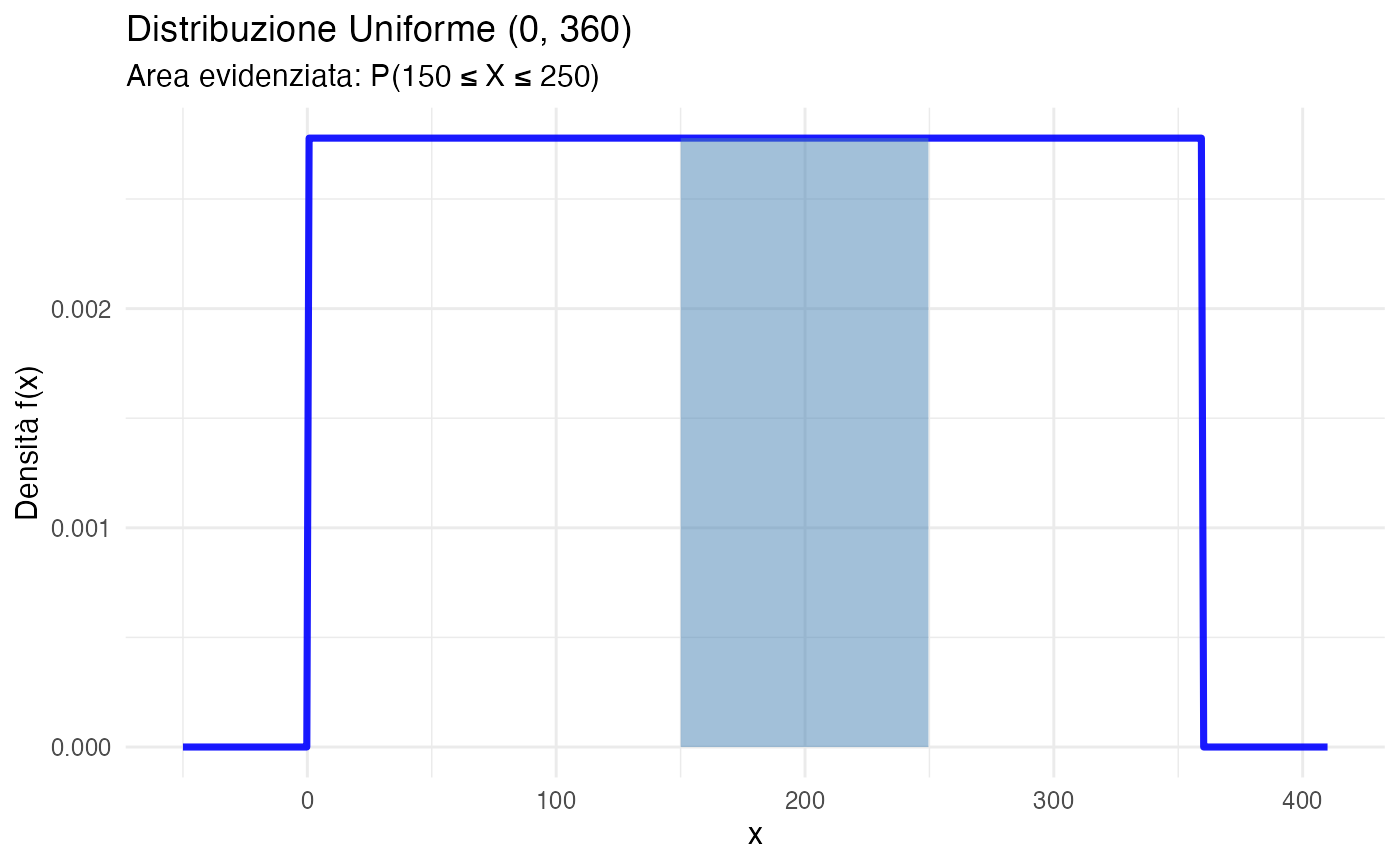
\includegraphics[width=0.85\linewidth,height=\textheight,keepaspectratio]{chapters/probability/13_cont_rv_distr_files/figure-pdf/unnamed-chunk-3-1.png}
\end{center}

\section{Distribuzione esponenziale}\label{distribuzione-esponenziale}

\subsection{Definizione e interpretazione
epistemica}\label{definizione-e-interpretazione-epistemica-6}

La distribuzione esponenziale modella il tempo di attesa fino al
verificarsi di un evento, assumendo che il tasso di occorrenza sia
costante nel tempo.

\begin{definition}[]\protect\hypertarget{def-exponential}{}\label{def-exponential}

Una variabile casuale \(X\) segue una distribuzione esponenziale con
parametro di tasso \(\lambda > 0\) se:

\[
X \sim \text{Exp}(\lambda), \quad f(x) = \lambda e^{-\lambda x} \text{ per } x \geq 0.
\]

\textbf{Proprietà}: \(\mathbb{E}(X) = \frac{1}{\lambda}\),
\(\mathbb{V}(X) = \frac{1}{\lambda^2}\).

\end{definition}

\textbf{Interpretazione epistemica}: il parametro \(\lambda\)
rappresenta il tasso atteso di occorrenza degli eventi per unità di
tempo. Un valore alto di \(\lambda\) indica eventi frequenti (tempi di
attesa brevi), mentre un valore basso indica eventi rari (tempi di
attesa lunghi).

\subsection{Proprietà di assenza di
memoria}\label{proprietuxe0-di-assenza-di-memoria}

La caratteristica distintiva dell'esponenziale è la \emph{proprietà di
assenza di memoria}: la probabilità che un evento si verifichi in un
intervallo futuro è indipendente dal tempo già trascorso. Formalmente:

\[
P(X > s + t \mid X > s) = P(X > t).
\]

Questa proprietà riflette l'assunzione che il processo non ``accumula''
né ``consuma'' probabilità con il passare del tempo: ogni istante è un
nuovo inizio.

\subsection{Ruolo nell'inferenza
bayesiana}\label{ruolo-nellinferenza-bayesiana-6}

La distribuzione esponenziale costituisce un caso particolare della
distribuzione gamma, formalmente esprimibile come
\(\text{Gamma}(1, \lambda)\). Nel contesto dell'inferenza bayesiana,
essa assume un duplice ruolo. In qualità di funzione di verosimiglianza,
viene tipicamente utilizzata per modellare variabili temporali continue,
come i tempi di attesa, le durate degli eventi o gli intervalli tra le
occorrenze successive. Per quanto riguarda l'aggiornamento bayesiano, la
distribuzione gamma rappresenta la distribuzione a priori coniugata per
il parametro di velocità \(\lambda\), consentendo così di ottenere una
distribuzione a posteriori in forma chiusa e appartenente alla stessa
famiglia distributiva.

\subsection{Esempio: tempi di attesa}\label{esempio-tempi-di-attesa}

\begin{Shaded}
\begin{Highlighting}[]
\CommentTok{\# Tempo medio di attesa: 4 giorni (lambda = 0.25)}
\NormalTok{lambda }\OtherTok{\textless{}{-}} \FloatTok{0.25}

\CommentTok{\# Probabilità di attesa ≤ 1.5 giorni}
\FunctionTok{cat}\NormalTok{(}\StringTok{"P(X ≤ 1.5) ="}\NormalTok{, }\FunctionTok{round}\NormalTok{(}\FunctionTok{pexp}\NormalTok{(}\FloatTok{1.5}\NormalTok{, }\AttributeTok{rate =}\NormalTok{ lambda), }\DecValTok{3}\NormalTok{), }\StringTok{"}\SpecialCharTok{\textbackslash{}n}\StringTok{"}\NormalTok{)}
\CommentTok{\#\textgreater{} P(X ≤ 1.5) = 0.313}

\CommentTok{\# Probabilità di attesa tra 1 e 6 giorni}
\FunctionTok{cat}\NormalTok{(}\StringTok{"P(1 ≤ X ≤ 6) ="}\NormalTok{, }\FunctionTok{round}\NormalTok{(}\FunctionTok{pexp}\NormalTok{(}\DecValTok{6}\NormalTok{, }\AttributeTok{rate =}\NormalTok{ lambda) }\SpecialCharTok{{-}} \FunctionTok{pexp}\NormalTok{(}\DecValTok{1}\NormalTok{, }\AttributeTok{rate =}\NormalTok{ lambda), }\DecValTok{3}\NormalTok{), }\StringTok{"}\SpecialCharTok{\textbackslash{}n}\StringTok{"}\NormalTok{)}
\CommentTok{\#\textgreater{} P(1 ≤ X ≤ 6) = 0.556}
\end{Highlighting}
\end{Shaded}

\begin{Shaded}
\begin{Highlighting}[]
\NormalTok{x }\OtherTok{\textless{}{-}} \FunctionTok{seq}\NormalTok{(}\DecValTok{0}\NormalTok{, }\DecValTok{20}\NormalTok{, }\AttributeTok{by =} \FloatTok{0.1}\NormalTok{)}
\NormalTok{pdf }\OtherTok{\textless{}{-}} \FunctionTok{dexp}\NormalTok{(x, }\AttributeTok{rate =}\NormalTok{ lambda)}

\FunctionTok{ggplot}\NormalTok{(}\FunctionTok{data.frame}\NormalTok{(}\AttributeTok{x =}\NormalTok{ x, }\AttributeTok{y =}\NormalTok{ pdf), }\FunctionTok{aes}\NormalTok{(}\AttributeTok{x =}\NormalTok{ x, }\AttributeTok{y =}\NormalTok{ y)) }\SpecialCharTok{+}
  \FunctionTok{geom\_line}\NormalTok{(}\AttributeTok{linewidth =} \FloatTok{1.2}\NormalTok{, }\AttributeTok{color =} \StringTok{"darkblue"}\NormalTok{) }\SpecialCharTok{+}
  \FunctionTok{geom\_area}\NormalTok{(}
    \AttributeTok{data =} \FunctionTok{subset}\NormalTok{(}\FunctionTok{data.frame}\NormalTok{(x, }\AttributeTok{y =}\NormalTok{ pdf), x }\SpecialCharTok{\textgreater{}=} \DecValTok{1} \SpecialCharTok{\&}\NormalTok{ x }\SpecialCharTok{\textless{}=} \DecValTok{6}\NormalTok{),}
    \AttributeTok{fill =} \StringTok{"steelblue"}\NormalTok{, }\AttributeTok{alpha =} \FloatTok{0.5}
\NormalTok{  ) }\SpecialCharTok{+}
  \FunctionTok{labs}\NormalTok{(}
    \AttributeTok{title =} \StringTok{"Distribuzione Esponenziale (λ = 0.25)"}\NormalTok{,}
    \AttributeTok{subtitle =} \StringTok{"Area evidenziata: P(1 ≤ X ≤ 6)"}\NormalTok{,}
    \AttributeTok{x =} \StringTok{"Tempo di attesa (giorni)"}\NormalTok{, }\AttributeTok{y =} \StringTok{"Densità"}
\NormalTok{  ) }\SpecialCharTok{+}
  \FunctionTok{theme\_minimal}\NormalTok{()}
\end{Highlighting}
\end{Shaded}

\begin{center}
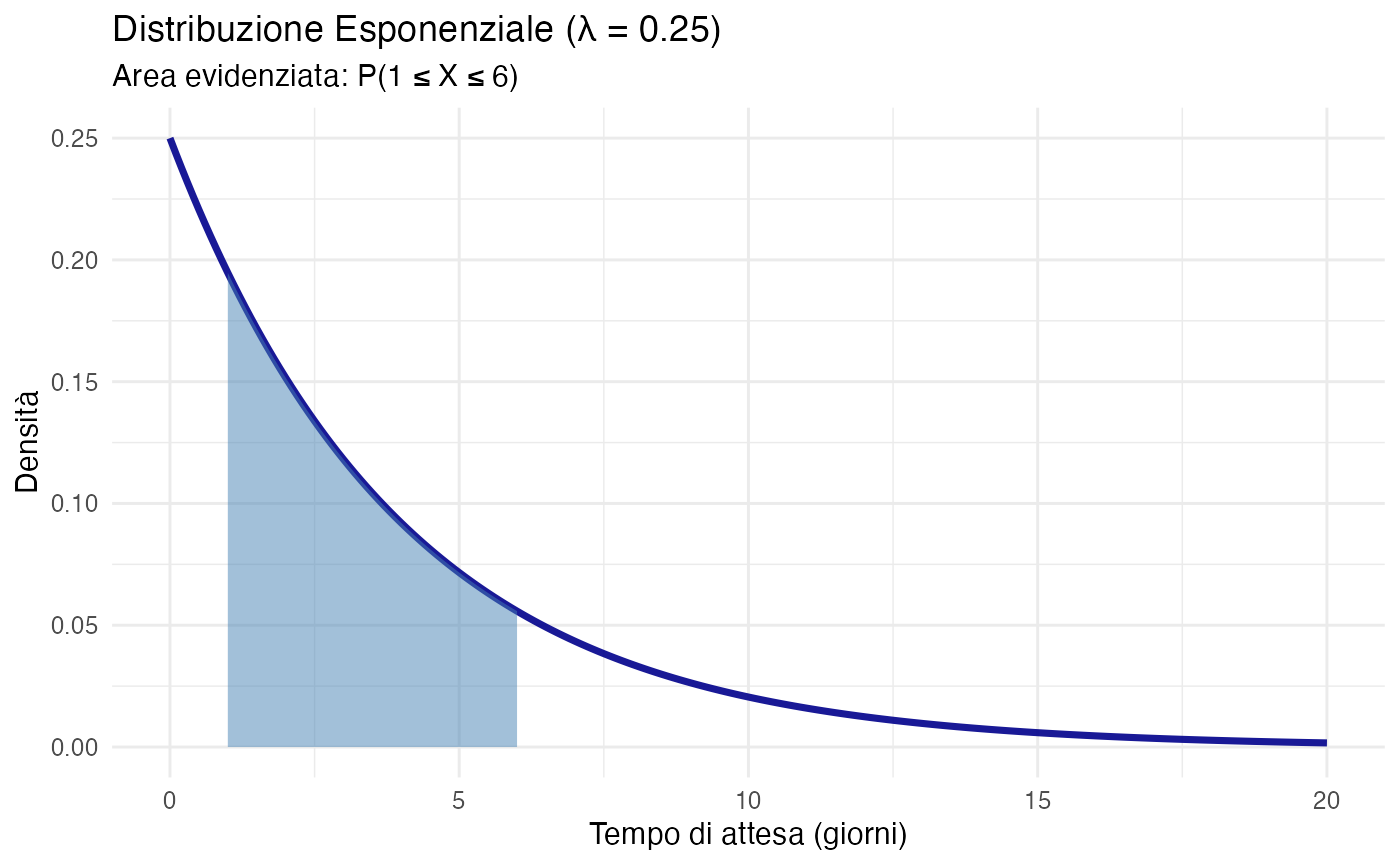
\includegraphics[width=0.85\linewidth,height=\textheight,keepaspectratio]{chapters/probability/13_cont_rv_distr_files/figure-pdf/unnamed-chunk-5-1.png}
\end{center}

\section{Distribuzione normale}\label{distribuzione-normale}

\subsection{Definizione e interpretazione
epistemica}\label{definizione-e-interpretazione-epistemica-7}

La distribuzione normale (o gaussiana) emerge naturalmente come
risultato della somma di molti effetti casuali indipendenti, un
principio formalizzato dal Teorema del Limite Centrale. Questa proprietà
la rende centrale nella modellazione di fenomeni psicologici influenzati
da molteplici fattori.

\begin{definition}[]\protect\hypertarget{def-normal}{}\label{def-normal}

Una variabile casuale \(Y\) segue una distribuzione normale con media
\(\mu\) e deviazione standard \(\sigma\) se:

\[
Y \sim \mathcal{N}(\mu, \sigma^2), \quad f(y) = \frac{1}{\sigma\sqrt{2\pi}} \exp\left(-\frac{(y - \mu)^2}{2\sigma^2}\right).
\]

\textbf{Proprietà}: \(\mathbb{E}(Y) = \mu\),
\(\mathbb{V}(Y) = \sigma^2\).

\end{definition}

\textbf{Interpretazione epistemica dei parametri}:

\begin{itemize}
\tightlist
\item
  il parametro \(\mu\) rappresenta il valore atteso, costituendo il
  ``centro di massa'' attorno al quale si concentrano le nostre
  credenze;
\item
  il parametro \(\sigma\) quantifica il grado di incertezza associato a
  tali credenze, indicando quanto riteniamo plausibile che i valori veri
  possano discostarsi dal valore centrale \(\mu\).
\end{itemize}

\subsection{Ruolo nell'inferenza
bayesiana}\label{ruolo-nellinferenza-bayesiana-7}

La distribuzione normale occupa una posizione centrale nell'inferenza
bayesiana e si rivela utile in molti contesti applicativi. In qualità di
verosimiglianza, viene comunemente impiegata per modellare una vasta
gamma di fenomeni continui, quali gli errori di misurazione, i punteggi
psicometrici e le variabili di natura biologica. Quando viene utilizzata
come distribuzione a priori per i parametri di posizione, nella forma
\(\mu \sim \mathcal{N}(\mu_0, \sigma_0^2)\), essa permette di esprimere
formalmente le credenze iniziali riguardo alla posizione del parametro
di interesse. Un'ulteriore proprietà che ne accresce l'utilità pratica è
la coniugazione: se la varianza \(\sigma^2\) è nota, la distribuzione
normale si configura come prior coniugata per il parametro \(\mu\),
garantendo che la distribuzione a posteriori appartenga alla stessa
famiglia distributiva.

\subsection{La regola 68-95-99.7}\label{la-regola-68-95-99.7}

La distribuzione normale possiede una proprietà universale che rimane
invariata indipendentemente dai valori specifici dei parametri \(\mu\) e
\(\sigma\). In particolare, si può affermare che approssimativamente il
68.3\% della massa probabilistica è concentrato entro un intervallo di
più o meno una deviazione standard dalla media, percentuale che sale al
95.4\% quando si considera un intervallo di due deviazioni standard e
raggiunge il 99.7\% per uno scarto di tre deviazioni standard.

Questa caratteristica fondamentale conferisce alla deviazione standard
il ruolo di unità di misura naturale per quantificare la ``distanza
dalla media'' in termini probabilistici, trasformandola da semplice
misura di dispersione a strumento per l'interpretazione probabilistica
della distribuzione.

\subsection{Il Teorema del Limite Centrale in
azione}\label{il-teorema-del-limite-centrale-in-azione}

La normale emerge dalla somma di effetti casuali indipendenti.
Visualizziamo questo fenomeno con una simulazione di passeggiate casuali
(\citeproc{ref-McElreath_rethinking}{McElreath, 2020}):

\begin{Shaded}
\begin{Highlighting}[]
\FunctionTok{set.seed}\NormalTok{(}\DecValTok{123}\NormalTok{)}
\NormalTok{n\_partecipanti }\OtherTok{\textless{}{-}} \DecValTok{1000}
\NormalTok{n\_passi }\OtherTok{\textless{}{-}} \DecValTok{16}

\CommentTok{\# Ogni partecipante compie 16 passi casuali in [{-}1, +1]}
\NormalTok{spostamenti }\OtherTok{\textless{}{-}} \FunctionTok{matrix}\NormalTok{(}\FunctionTok{runif}\NormalTok{(n\_partecipanti }\SpecialCharTok{*}\NormalTok{ n\_passi, }\AttributeTok{min =} \SpecialCharTok{{-}}\DecValTok{1}\NormalTok{, }\AttributeTok{max =} \DecValTok{1}\NormalTok{), }\AttributeTok{ncol =}\NormalTok{ n\_passi)}
\NormalTok{posizioni\_finali }\OtherTok{\textless{}{-}} \FunctionTok{rowSums}\NormalTok{(spostamenti)}

\CommentTok{\# Visualizzazione}
\FunctionTok{ggplot}\NormalTok{(}\FunctionTok{data.frame}\NormalTok{(}\AttributeTok{Posizione =}\NormalTok{ posizioni\_finali), }\FunctionTok{aes}\NormalTok{(}\AttributeTok{x =}\NormalTok{ Posizione)) }\SpecialCharTok{+}
  \FunctionTok{geom\_histogram}\NormalTok{(}\FunctionTok{aes}\NormalTok{(}\AttributeTok{y =} \FunctionTok{after\_stat}\NormalTok{(density)), }\AttributeTok{bins =} \DecValTok{30}\NormalTok{, }\AttributeTok{fill =} \StringTok{"lightblue"}\NormalTok{, }\AttributeTok{alpha =} \FloatTok{0.7}\NormalTok{) }\SpecialCharTok{+}
  \FunctionTok{stat\_function}\NormalTok{(}
    \AttributeTok{fun =}\NormalTok{ dnorm, }
    \AttributeTok{args =} \FunctionTok{list}\NormalTok{(}\AttributeTok{mean =} \FunctionTok{mean}\NormalTok{(posizioni\_finali), }\AttributeTok{sd =} \FunctionTok{sd}\NormalTok{(posizioni\_finali)), }
    \AttributeTok{color =} \StringTok{"red"}\NormalTok{, }\AttributeTok{linewidth =} \DecValTok{1}
\NormalTok{  ) }\SpecialCharTok{+}
  \FunctionTok{labs}\NormalTok{(}
    \AttributeTok{title =} \StringTok{"Teorema del Limite Centrale"}\NormalTok{,}
    \AttributeTok{subtitle =} \StringTok{"Somma di 16 variabili uniformi converge alla normale"}\NormalTok{,}
    \AttributeTok{x =} \StringTok{"Posizione finale"}\NormalTok{, }\AttributeTok{y =} \StringTok{"Densità"}
\NormalTok{  ) }\SpecialCharTok{+}
  \FunctionTok{theme\_minimal}\NormalTok{()}
\end{Highlighting}
\end{Shaded}

\begin{center}
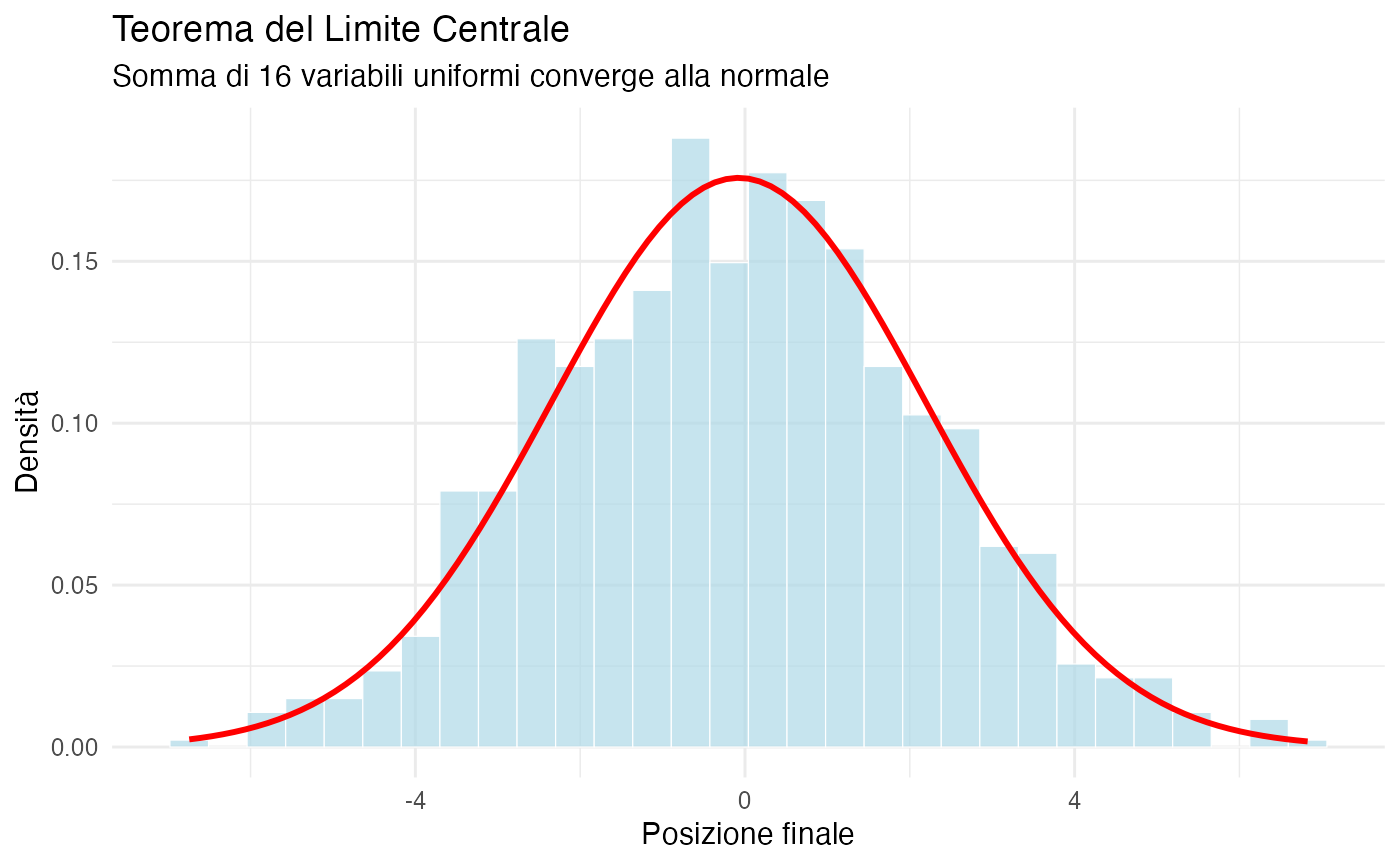
\includegraphics[width=0.85\linewidth,height=\textheight,keepaspectratio]{chapters/probability/13_cont_rv_distr_files/figure-pdf/unnamed-chunk-6-1.png}
\end{center}

Nonostante ogni singolo passo segua una distribuzione uniforme, la
distribuzione delle posizioni finali approssima una distribuzione
normale, dimostrando empiricamente il TLC.

\subsection{Visualizzazione degli intervalli di
credibilità}\label{visualizzazione-degli-intervalli-di-credibilituxe0}

\begin{Shaded}
\begin{Highlighting}[]
\NormalTok{mu }\OtherTok{\textless{}{-}} \DecValTok{100}
\NormalTok{sigma }\OtherTok{\textless{}{-}} \DecValTok{15}
\NormalTok{x }\OtherTok{\textless{}{-}} \FunctionTok{seq}\NormalTok{(mu }\SpecialCharTok{{-}} \DecValTok{4}\SpecialCharTok{*}\NormalTok{sigma, mu }\SpecialCharTok{+} \DecValTok{4}\SpecialCharTok{*}\NormalTok{sigma, }\AttributeTok{length.out =} \DecValTok{1000}\NormalTok{)}
\NormalTok{df }\OtherTok{\textless{}{-}} \FunctionTok{data.frame}\NormalTok{(}\AttributeTok{x =}\NormalTok{ x, }\AttributeTok{pdf =} \FunctionTok{dnorm}\NormalTok{(x, mu, sigma))}

\FunctionTok{ggplot}\NormalTok{(df, }\FunctionTok{aes}\NormalTok{(}\AttributeTok{x =}\NormalTok{ x, }\AttributeTok{y =}\NormalTok{ pdf)) }\SpecialCharTok{+}
  \FunctionTok{geom\_line}\NormalTok{(}\AttributeTok{color =} \StringTok{"blue"}\NormalTok{) }\SpecialCharTok{+}
  \FunctionTok{geom\_area}\NormalTok{(}
    \AttributeTok{data =} \FunctionTok{subset}\NormalTok{(df, x }\SpecialCharTok{\textgreater{}=}\NormalTok{ mu }\SpecialCharTok{{-}} \FloatTok{1.96}\SpecialCharTok{*}\NormalTok{sigma }\SpecialCharTok{\&}\NormalTok{ x }\SpecialCharTok{\textless{}=}\NormalTok{ mu }\SpecialCharTok{+} \FloatTok{1.96}\SpecialCharTok{*}\NormalTok{sigma),}
    \AttributeTok{fill =} \StringTok{"steelblue"}\NormalTok{, }\AttributeTok{alpha =} \FloatTok{0.5}
\NormalTok{  ) }\SpecialCharTok{+}
  \FunctionTok{labs}\NormalTok{(}
    \AttributeTok{title =} \StringTok{"Distribuzione Normale (μ = 100, σ = 15)"}\NormalTok{,}
    \AttributeTok{subtitle =} \StringTok{"Il 95\% della massa si trova entro ±1.96σ dalla media"}\NormalTok{,}
    \AttributeTok{x =} \StringTok{"Valori"}\NormalTok{, }\AttributeTok{y =} \StringTok{"Densità"}
\NormalTok{  ) }\SpecialCharTok{+}
  \FunctionTok{theme\_minimal}\NormalTok{()}
\end{Highlighting}
\end{Shaded}

\begin{center}
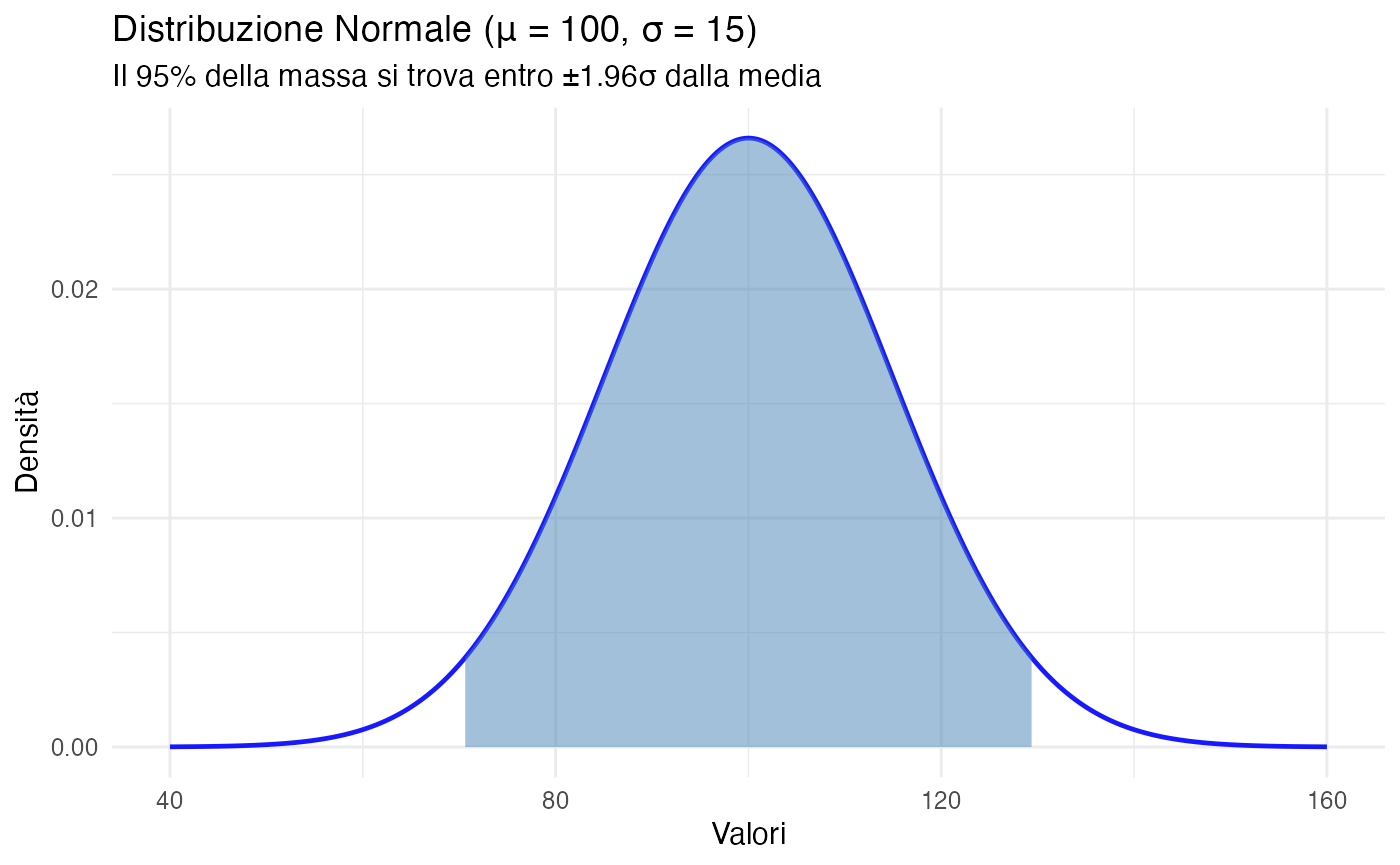
\includegraphics[width=0.85\linewidth,height=\textheight,keepaspectratio]{chapters/probability/13_cont_rv_distr_files/figure-pdf/unnamed-chunk-7-1.png}
\end{center}

\section{Distribuzione chi-quadrato}\label{distribuzione-chi-quadrato}

\subsection{Definizione e interpretazione
epistemica}\label{definizione-e-interpretazione-epistemica-8}

La distribuzione chi-quadrato emerge dalla somma dei quadrati di
variabili normali standard indipendenti.

\begin{definition}[]\protect\hypertarget{def-chisq}{}\label{def-chisq}

Se \(Z_1, \ldots, Z_k\) sono variabili casuali i.i.d. con distribuzione
\(\mathcal{N}(0, 1)\), allora:

\[
X = Z_1^2 + Z_2^2 + \cdots + Z_k^2 \sim \chi^2_k
\]

dove \(k\) sono i \emph{gradi di libertà}.

\textbf{Proprietà}: \(\mathbb{E}(X) = k\), \(\mathbb{V}(X) = 2k\).

\end{definition}

\textbf{Interpretazione epistemica}: la distribuzione chi-quadrato
quantifica la ``dispersione quadratica'' delle variabili normali. I
gradi di libertà \(k\) determinano quante fonti indipendenti di
variazione contribuiscono alla somma.

\subsection{Ruolo nell'inferenza
bayesiana}\label{ruolo-nellinferenza-bayesiana-8}

La distribuzione chi-quadrato è un caso particolare della distribuzione
gamma, essendo formalmente equivalente a
\(\chi^2_k = \text{Gamma}(k/2, 1/2)\). Nell'ambito dell'inferenza
bayesiana, questa distribuzione ricopre un ruolo in diversi contesti.
Emerge naturalmente nella modellazione delle varianze campionarie,
fornendo una base teorica per l'analisi della variabilità dei dati. La
sua trasformazione inversa, nota come distribuzione chi-quadrato
inversa, costituisce la distribuzione a priori coniugata per il
parametro di varianza \(\sigma^2\) nel modello normale con media nota,
facilitando l'aggiornamento bayesiano in forma chiusa. Inoltre, la
distribuzione chi-quadrato compare implicitamente in molte strutture
modellistiche gerarchiche, in particolare quando si intende
rappresentare formalmente l'incertezza associata al parametro di
precisione.

\subsection{Visualizzazione}\label{visualizzazione-1}

\begin{Shaded}
\begin{Highlighting}[]
\NormalTok{x }\OtherTok{\textless{}{-}} \FunctionTok{seq}\NormalTok{(}\DecValTok{0}\NormalTok{, }\DecValTok{40}\NormalTok{, }\AttributeTok{by =} \FloatTok{0.1}\NormalTok{)}
\NormalTok{nus }\OtherTok{\textless{}{-}} \FunctionTok{c}\NormalTok{(}\DecValTok{2}\NormalTok{, }\DecValTok{4}\NormalTok{, }\DecValTok{8}\NormalTok{, }\DecValTok{16}\NormalTok{)}

\NormalTok{data }\OtherTok{\textless{}{-}} \FunctionTok{do.call}\NormalTok{(rbind, }\FunctionTok{lapply}\NormalTok{(nus, }\ControlFlowTok{function}\NormalTok{(nu) \{}
  \FunctionTok{data.frame}\NormalTok{(}\AttributeTok{x =}\NormalTok{ x, }\AttributeTok{f\_x =} \FunctionTok{dchisq}\NormalTok{(x, }\AttributeTok{df =}\NormalTok{ nu), }\AttributeTok{nu =} \FunctionTok{as.factor}\NormalTok{(nu))}
\NormalTok{\}))}

\FunctionTok{ggplot}\NormalTok{(data, }\FunctionTok{aes}\NormalTok{(}\AttributeTok{x =}\NormalTok{ x, }\AttributeTok{y =}\NormalTok{ f\_x, }\AttributeTok{color =}\NormalTok{ nu)) }\SpecialCharTok{+}
  \FunctionTok{geom\_line}\NormalTok{(}\AttributeTok{linewidth =} \DecValTok{1}\NormalTok{) }\SpecialCharTok{+}
  \FunctionTok{labs}\NormalTok{(}
    \AttributeTok{title =} \StringTok{"Distribuzione Chi{-}Quadrato"}\NormalTok{,}
    \AttributeTok{subtitle =} \StringTok{"La forma diventa più simmetrica al crescere dei gradi di libertà"}\NormalTok{,}
    \AttributeTok{x =} \StringTok{"x"}\NormalTok{, }\AttributeTok{y =} \StringTok{"f(x)"}\NormalTok{, }\AttributeTok{color =} \StringTok{"ν"}
\NormalTok{  ) }\SpecialCharTok{+}
  \FunctionTok{theme\_minimal}\NormalTok{()}
\end{Highlighting}
\end{Shaded}

\begin{center}
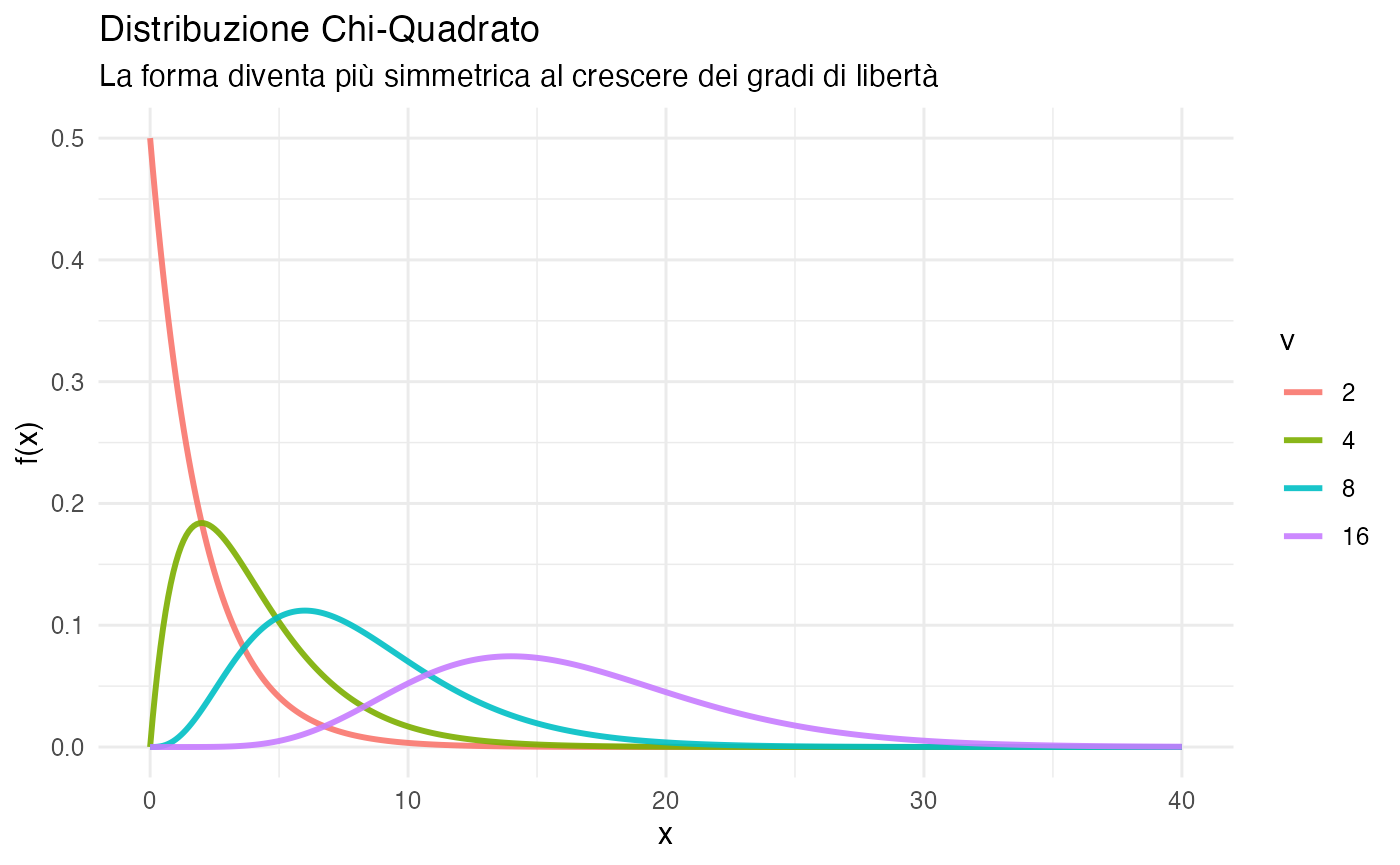
\includegraphics[width=0.85\linewidth,height=\textheight,keepaspectratio]{chapters/probability/13_cont_rv_distr_files/figure-pdf/unnamed-chunk-8-1.png}
\end{center}

\section{\texorpdfstring{Distribuzione \(t\) di
Student}{Distribuzione t di Student}}\label{distribuzione-t-di-student}

\subsection{Definizione e interpretazione
epistemica}\label{definizione-e-interpretazione-epistemica-9}

La distribuzione \(t\) di Student emerge quando si standardizza una
variabile aleatoria normale utilizzando una stima campionaria della sua
varianza, derivante da un campione finito.

\begin{definition}[]\protect\hypertarget{def-t-student}{}\label{def-t-student}

Date due variabili aleatorie indipendenti \(Z \sim \mathcal{N}(0, 1)\) e
\(W \sim \chi^2_\nu\), la variabile risultante dalla trasformazione:

\[
T = \frac{Z}{\sqrt{W/\nu}} \sim t_\nu
\] segue una distribuzione \(t\) di Student con \(\nu\) gradi di
libertà.

\textbf{Proprietà}: \(\mathbb{E}(T) = 0\) per \(\nu > 1\);
\(\mathbb{V}(T) = \frac{\nu}{\nu - 2}\) per \(\nu > 2\).

\end{definition}

\textbf{Interpretazione epistemica}: la \(t\) di Student ha \textbf{code
più pesanti della normale}, riflettendo l'incertezza aggiuntiva
derivante dal non conoscere con certezza la varianza. Man mano che
\(\nu\) aumenta, questa incertezza diminuisce e la \(t\) tende alla
distribuzione normale.

\subsection{Ruolo nell'inferenza
bayesiana}\label{ruolo-nellinferenza-bayesiana-9}

La distribuzione \(t\) di Student riveste un ruolo di particolare
rilievo nell'inferenza bayesiana per tre motivi. In primo luogo, funge
da distribuzione a priori robusta per i parametri di posizione:
l'utilizzo di una distribuzione \(t_\nu(\mu_0, \sigma_0)\) come prior
per la media assegna infatti una maggiore plausibilità ai valori estremi
rispetto a una distribuzione normale, conferendo al modello una maggiore
resistenza all'influenza potenziale di osservazioni anomale.

In secondo luogo, la distribuzione \(t\) emerge naturalmente come
distribuzione predittiva quando si considera l'incertezza congiunta sia
sulla media che sulla varianza di un modello normale. In tali
circostanze, la distribuzione predittiva marginale per le nuove
osservazioni assume la forma di una distribuzione t di Student, a
differenza di quanto avverrebbe nel caso in cui la varianza fosse nota.

Infine, la distribuzione \(t\) si presta efficacemente come scelta per
le distribuzioni a priori debolmente informative. Specificando un numero
ridotto di gradi di libertà, come ad esempio \(\nu = 3\) o il caso
limite \(\nu = 1\), corrispondente alla distribuzione di Cauchy, è
possibile definire prior che, pur incorporando informazioni di
regolarizzazione, non tenderanno a dominare l'evidenza portata dai dati,
nemmeno in contesti caratterizzati da campioni di piccole dimensioni.

\subsection{Confronto con la normale}\label{confronto-con-la-normale}

\begin{Shaded}
\begin{Highlighting}[]
\NormalTok{x }\OtherTok{\textless{}{-}} \FunctionTok{seq}\NormalTok{(}\SpecialCharTok{{-}}\DecValTok{4}\NormalTok{, }\DecValTok{4}\NormalTok{, }\AttributeTok{length.out =} \DecValTok{1000}\NormalTok{)}
\NormalTok{gradi\_liberta }\OtherTok{\textless{}{-}} \FunctionTok{c}\NormalTok{(}\DecValTok{1}\NormalTok{, }\DecValTok{3}\NormalTok{, }\DecValTok{10}\NormalTok{)}

\NormalTok{dati\_plot }\OtherTok{\textless{}{-}} \FunctionTok{data.frame}\NormalTok{(}
  \AttributeTok{x =} \FunctionTok{rep}\NormalTok{(x, }\FunctionTok{length}\NormalTok{(gradi\_liberta) }\SpecialCharTok{+} \DecValTok{1}\NormalTok{),}
  \AttributeTok{densita =} \FunctionTok{c}\NormalTok{(}
    \FunctionTok{dnorm}\NormalTok{(x),}
    \FunctionTok{dt}\NormalTok{(x, }\AttributeTok{df =}\NormalTok{ gradi\_liberta[}\DecValTok{1}\NormalTok{]),}
    \FunctionTok{dt}\NormalTok{(x, }\AttributeTok{df =}\NormalTok{ gradi\_liberta[}\DecValTok{2}\NormalTok{]),}
    \FunctionTok{dt}\NormalTok{(x, }\AttributeTok{df =}\NormalTok{ gradi\_liberta[}\DecValTok{3}\NormalTok{])}
\NormalTok{  ),}
  \AttributeTok{distribuzione =} \FunctionTok{rep}\NormalTok{(}
    \FunctionTok{c}\NormalTok{(}\StringTok{"Normale"}\NormalTok{, }\FunctionTok{paste0}\NormalTok{(}\StringTok{"t (ν = "}\NormalTok{, gradi\_liberta, }\StringTok{")"}\NormalTok{)), }
    \AttributeTok{each =} \FunctionTok{length}\NormalTok{(x)}
\NormalTok{  )}
\NormalTok{)}

\FunctionTok{ggplot}\NormalTok{(dati\_plot, }\FunctionTok{aes}\NormalTok{(}\AttributeTok{x =}\NormalTok{ x, }\AttributeTok{y =}\NormalTok{ densita, }\AttributeTok{color =}\NormalTok{ distribuzione)) }\SpecialCharTok{+}
  \FunctionTok{geom\_line}\NormalTok{(}\AttributeTok{linewidth =} \DecValTok{1}\NormalTok{) }\SpecialCharTok{+}
  \FunctionTok{labs}\NormalTok{(}
    \AttributeTok{title =} \StringTok{"Confronto t di Student e Normale"}\NormalTok{,}
    \AttributeTok{subtitle =} \StringTok{"Code più pesanti per ν piccoli; convergenza alla normale per ν → ∞"}\NormalTok{,}
    \AttributeTok{x =} \StringTok{"Valore"}\NormalTok{, }\AttributeTok{y =} \StringTok{"Densità"}\NormalTok{, }\AttributeTok{color =} \StringTok{"Distribuzione"}
\NormalTok{  ) }\SpecialCharTok{+}
  \FunctionTok{theme\_minimal}\NormalTok{() }\SpecialCharTok{+}
  \FunctionTok{scale\_color\_brewer}\NormalTok{(}\AttributeTok{palette =} \StringTok{"Set1"}\NormalTok{)}
\end{Highlighting}
\end{Shaded}

\begin{center}
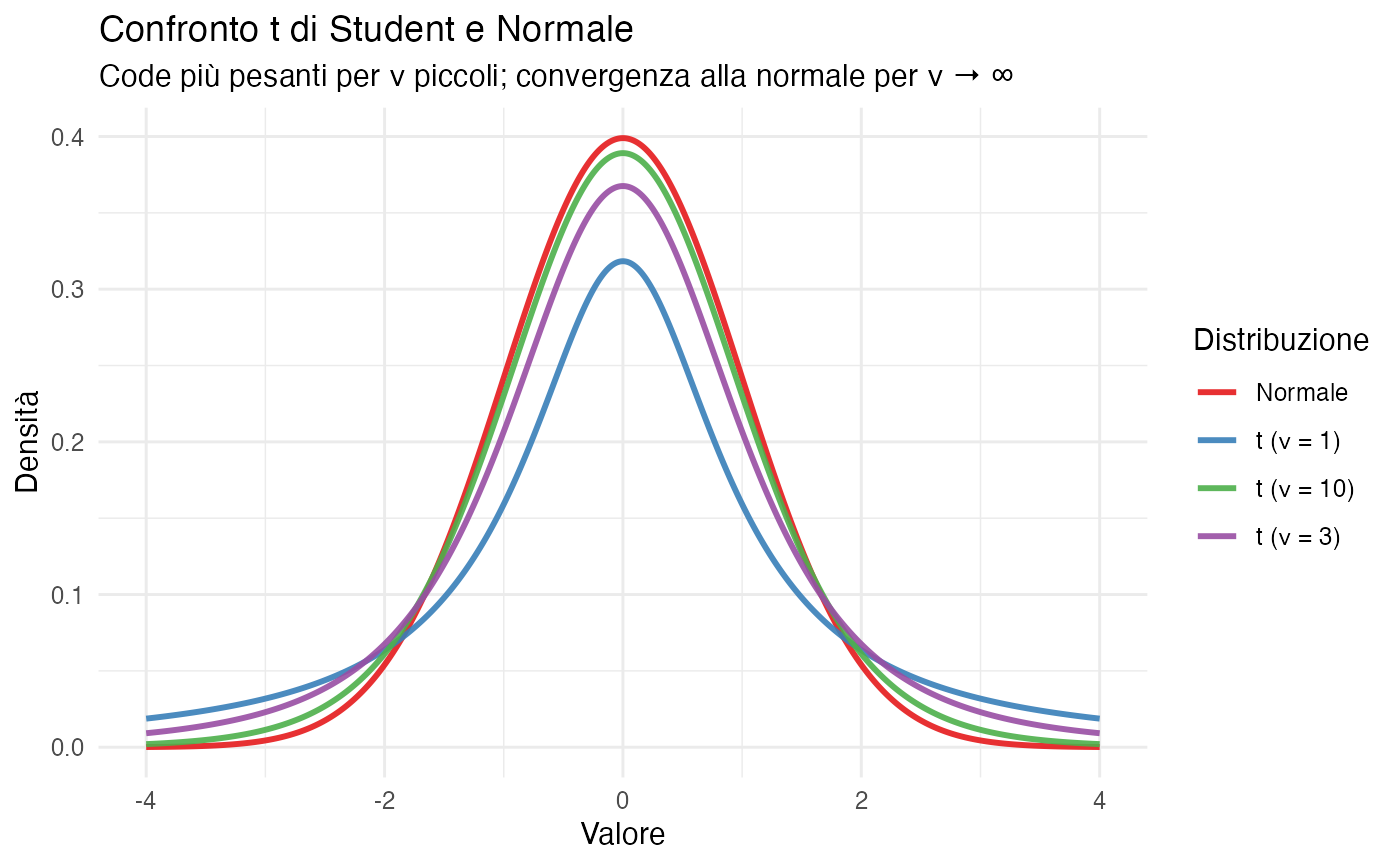
\includegraphics[width=0.85\linewidth,height=\textheight,keepaspectratio]{chapters/probability/13_cont_rv_distr_files/figure-pdf/unnamed-chunk-9-1.png}
\end{center}

\section{Distribuzione beta}\label{distribuzione-beta}

\subsection{Definizione e interpretazione
epistemica}\label{definizione-e-interpretazione-epistemica-10}

La distribuzione beta è la scelta naturale per rappresentare credenze su
proporzioni o probabilità, ovvero quantità vincolate all'intervallo
\((0, 1)\).

\begin{definition}[]\protect\hypertarget{def-beta}{}\label{def-beta}

Una variabile casuale \(\theta\) segue una distribuzione beta con
parametri \(\alpha > 0\) e \(\beta > 0\) se:

\[
\theta \sim \text{Beta}(\alpha, \beta), \quad f(\theta) = \frac{\theta^{\alpha-1}(1-\theta)^{\beta-1}}{B(\alpha, \beta)},
\] dove \(B(\alpha, \beta)\) è la funzione beta di Eulero.

\textbf{Proprietà}:

\begin{itemize}
\tightlist
\item
  \(\mathbb{E}(\theta) = \frac{\alpha}{\alpha + \beta}\);
\item
  \(\mathbb{V}(\theta) = \frac{\alpha\beta}{(\alpha + \beta)^2(\alpha + \beta + 1)}\);
\item
  Moda (per \(\alpha, \beta > 1\)):
  \(\frac{\alpha - 1}{\alpha + \beta - 2}\).
\end{itemize}

\end{definition}

\textbf{Interpretazione epistemica dei parametri}: i parametri
\(\alpha\) e \(\beta\) della distribuzione beta ammettono
un'interpretazione epistemica particolarmente intuitiva in termini di
``pseudo-osservazioni''. In questa prospettiva, \(\alpha - 1\)
rappresenta il numero ipotetico di successi precedentemente osservati,
mentre \(\beta - 1\) corrisponde al numero analogo di insuccessi. Questa
caratteristica consente di incorporare in modo trasparente
l'informazione a priori nel modello. Il caso particolare
\(\alpha = \beta = 1\) assume un significato speciale, in quanto produce
una distribuzione uniforme che rappresenta formalmente uno stato di
massima ignoranza riguardo al parametro di interesse.

\subsection{Ruolo nell'inferenza
bayesiana}\label{ruolo-nellinferenza-bayesiana-10}

La beta è la \textbf{prior coniugata} per il parametro \(p\) della
distribuzione binomiale:

\[
\text{Prior: } p \sim \text{Beta}(\alpha, \beta), \quad \text{Dati: } k \text{ successi su } n \text{ prove}.
\] \[
\text{Posterior: } p \mid k \sim \text{Beta}(\alpha + k, \beta + n - k).
\]

Questa proprietà rende l'aggiornamento bayesiano analiticamente
trattabile: i parametri della distribuzione a posteriori si ottengono
semplicemente sommando i conteggi osservati agli pseudo-conteggi della
distribuzione a priori.

\subsection{Flessibilità della forma}\label{flessibilituxe0-della-forma}

La distribuzione beta può assumere forme molto diverse a seconda dei
parametri:

\begin{Shaded}
\begin{Highlighting}[]
\NormalTok{x }\OtherTok{\textless{}{-}} \FunctionTok{seq}\NormalTok{(}\DecValTok{0}\NormalTok{, }\DecValTok{1}\NormalTok{, }\AttributeTok{length.out =} \DecValTok{200}\NormalTok{)}
\NormalTok{params }\OtherTok{\textless{}{-}} \FunctionTok{list}\NormalTok{(}
  \FunctionTok{c}\NormalTok{(}\FloatTok{0.5}\NormalTok{, }\FloatTok{0.5}\NormalTok{), }\FunctionTok{c}\NormalTok{(}\DecValTok{1}\NormalTok{, }\DecValTok{1}\NormalTok{), }\FunctionTok{c}\NormalTok{(}\DecValTok{2}\NormalTok{, }\DecValTok{2}\NormalTok{), }\FunctionTok{c}\NormalTok{(}\DecValTok{2}\NormalTok{, }\DecValTok{5}\NormalTok{), }\FunctionTok{c}\NormalTok{(}\DecValTok{5}\NormalTok{, }\DecValTok{2}\NormalTok{)}
\NormalTok{)}

\NormalTok{df }\OtherTok{\textless{}{-}} \FunctionTok{do.call}\NormalTok{(rbind, }\FunctionTok{lapply}\NormalTok{(params, }\ControlFlowTok{function}\NormalTok{(p) \{}
  \FunctionTok{data.frame}\NormalTok{(}
    \AttributeTok{x =}\NormalTok{ x,}
    \AttributeTok{density =} \FunctionTok{dbeta}\NormalTok{(x, p[}\DecValTok{1}\NormalTok{], p[}\DecValTok{2}\NormalTok{]),}
    \AttributeTok{label =} \FunctionTok{paste0}\NormalTok{(}\StringTok{"α = "}\NormalTok{, p[}\DecValTok{1}\NormalTok{], }\StringTok{", β = "}\NormalTok{, p[}\DecValTok{2}\NormalTok{])}
\NormalTok{  )}
\NormalTok{\}))}

\FunctionTok{ggplot}\NormalTok{(df, }\FunctionTok{aes}\NormalTok{(}\AttributeTok{x =}\NormalTok{ x, }\AttributeTok{y =}\NormalTok{ density, }\AttributeTok{color =}\NormalTok{ label)) }\SpecialCharTok{+}
  \FunctionTok{geom\_line}\NormalTok{(}\AttributeTok{linewidth =} \DecValTok{1}\NormalTok{) }\SpecialCharTok{+}
  \FunctionTok{labs}\NormalTok{(}
    \AttributeTok{title =} \StringTok{"Flessibilità della distribuzione Beta"}\NormalTok{,}
    \AttributeTok{subtitle =} \StringTok{"Diverse combinazioni di parametri producono forme radicalmente diverse"}\NormalTok{,}
    \AttributeTok{x =} \StringTok{"θ"}\NormalTok{, }\AttributeTok{y =} \StringTok{"f(θ)"}
\NormalTok{  ) }\SpecialCharTok{+}
  \FunctionTok{theme\_minimal}\NormalTok{() }\SpecialCharTok{+}
  \FunctionTok{theme}\NormalTok{(}\AttributeTok{legend.title =} \FunctionTok{element\_blank}\NormalTok{())}
\end{Highlighting}
\end{Shaded}

\begin{center}
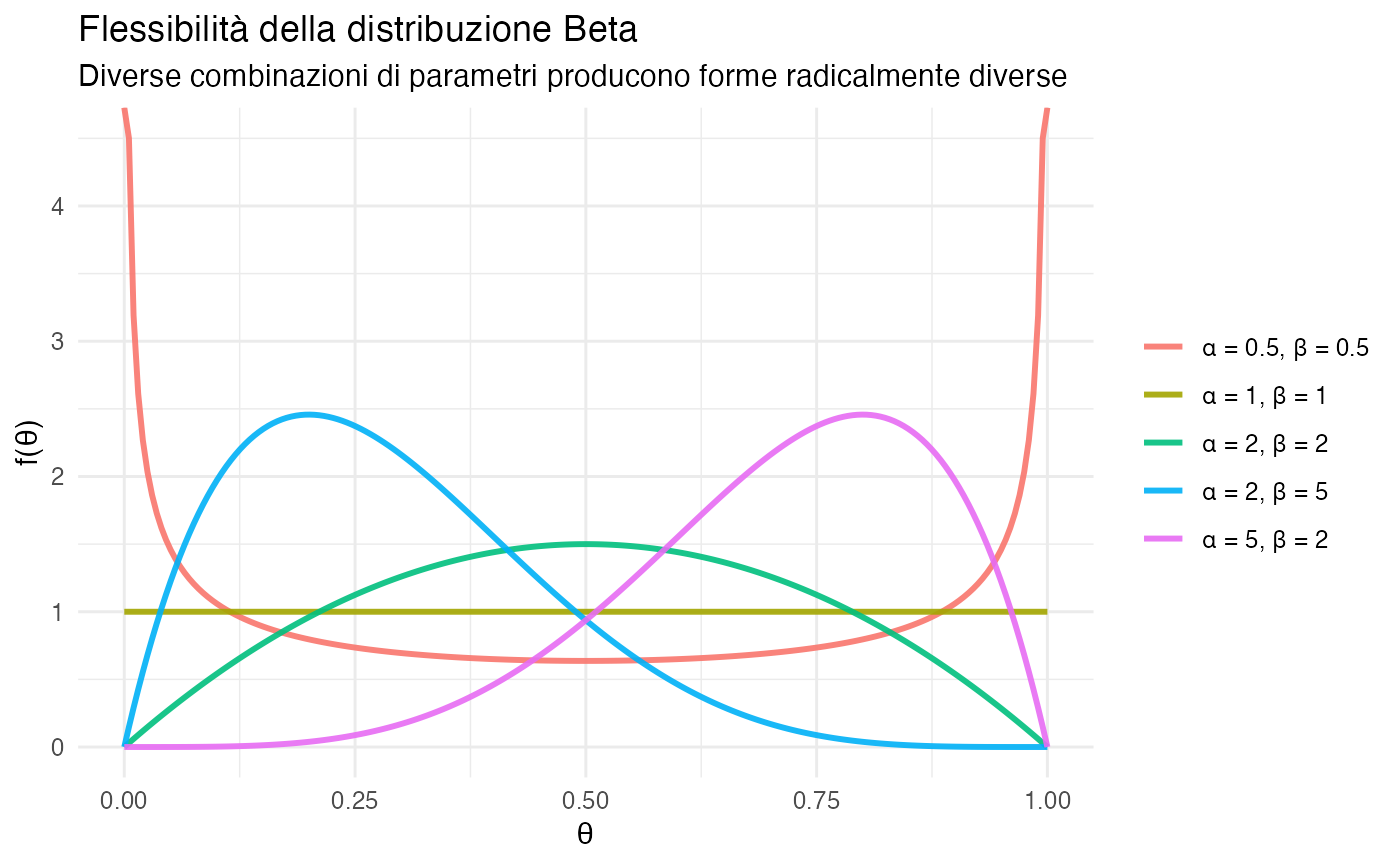
\includegraphics[width=0.85\linewidth,height=\textheight,keepaspectratio]{chapters/probability/13_cont_rv_distr_files/figure-pdf/unnamed-chunk-10-1.png}
\end{center}

\subsection{Esempio: aggiornamento
bayesiano}\label{esempio-aggiornamento-bayesiano-1}

\begin{Shaded}
\begin{Highlighting}[]
\CommentTok{\# Prior: Beta(2, 2) {-} credenza iniziale moderatamente incerta}
\NormalTok{alpha\_prior }\OtherTok{\textless{}{-}} \DecValTok{2}
\NormalTok{beta\_prior }\OtherTok{\textless{}{-}} \DecValTok{2}

\CommentTok{\# Dati osservati: 7 successi su 10 prove}
\NormalTok{successi }\OtherTok{\textless{}{-}} \DecValTok{7}
\NormalTok{prove }\OtherTok{\textless{}{-}} \DecValTok{10}

\CommentTok{\# Posterior: Beta(2+7, 2+3) = Beta(9, 5)}
\NormalTok{alpha\_post }\OtherTok{\textless{}{-}}\NormalTok{ alpha\_prior }\SpecialCharTok{+}\NormalTok{ successi}
\NormalTok{beta\_post }\OtherTok{\textless{}{-}}\NormalTok{ beta\_prior }\SpecialCharTok{+}\NormalTok{ (prove }\SpecialCharTok{{-}}\NormalTok{ successi)}

\CommentTok{\# Visualizzazione}
\NormalTok{x }\OtherTok{\textless{}{-}} \FunctionTok{seq}\NormalTok{(}\DecValTok{0}\NormalTok{, }\DecValTok{1}\NormalTok{, }\AttributeTok{length.out =} \DecValTok{200}\NormalTok{)}
\NormalTok{df }\OtherTok{\textless{}{-}} \FunctionTok{data.frame}\NormalTok{(}
  \AttributeTok{x =} \FunctionTok{rep}\NormalTok{(x, }\DecValTok{2}\NormalTok{),}
  \AttributeTok{density =} \FunctionTok{c}\NormalTok{(}\FunctionTok{dbeta}\NormalTok{(x, alpha\_prior, beta\_prior), }\FunctionTok{dbeta}\NormalTok{(x, alpha\_post, beta\_post)),}
  \AttributeTok{tipo =} \FunctionTok{rep}\NormalTok{(}\FunctionTok{c}\NormalTok{(}\StringTok{"Prior Beta(2,2)"}\NormalTok{, }\StringTok{"Posterior Beta(9,5)"}\NormalTok{), }\AttributeTok{each =} \FunctionTok{length}\NormalTok{(x))}
\NormalTok{)}

\FunctionTok{ggplot}\NormalTok{(df, }\FunctionTok{aes}\NormalTok{(}\AttributeTok{x =}\NormalTok{ x, }\AttributeTok{y =}\NormalTok{ density, }\AttributeTok{color =}\NormalTok{ tipo)) }\SpecialCharTok{+}
  \FunctionTok{geom\_line}\NormalTok{(}\AttributeTok{linewidth =} \FloatTok{1.2}\NormalTok{) }\SpecialCharTok{+}
  \FunctionTok{labs}\NormalTok{(}
    \AttributeTok{title =} \StringTok{"Aggiornamento Bayesiano: Beta{-}Binomiale"}\NormalTok{,}
    \AttributeTok{subtitle =} \StringTok{"7 successi su 10 prove aggiornano la prior"}\NormalTok{,}
    \AttributeTok{x =} \StringTok{"p"}\NormalTok{, }\AttributeTok{y =} \StringTok{"Densità"}
\NormalTok{  ) }\SpecialCharTok{+}
  \FunctionTok{theme\_minimal}\NormalTok{()}
\end{Highlighting}
\end{Shaded}

\begin{center}
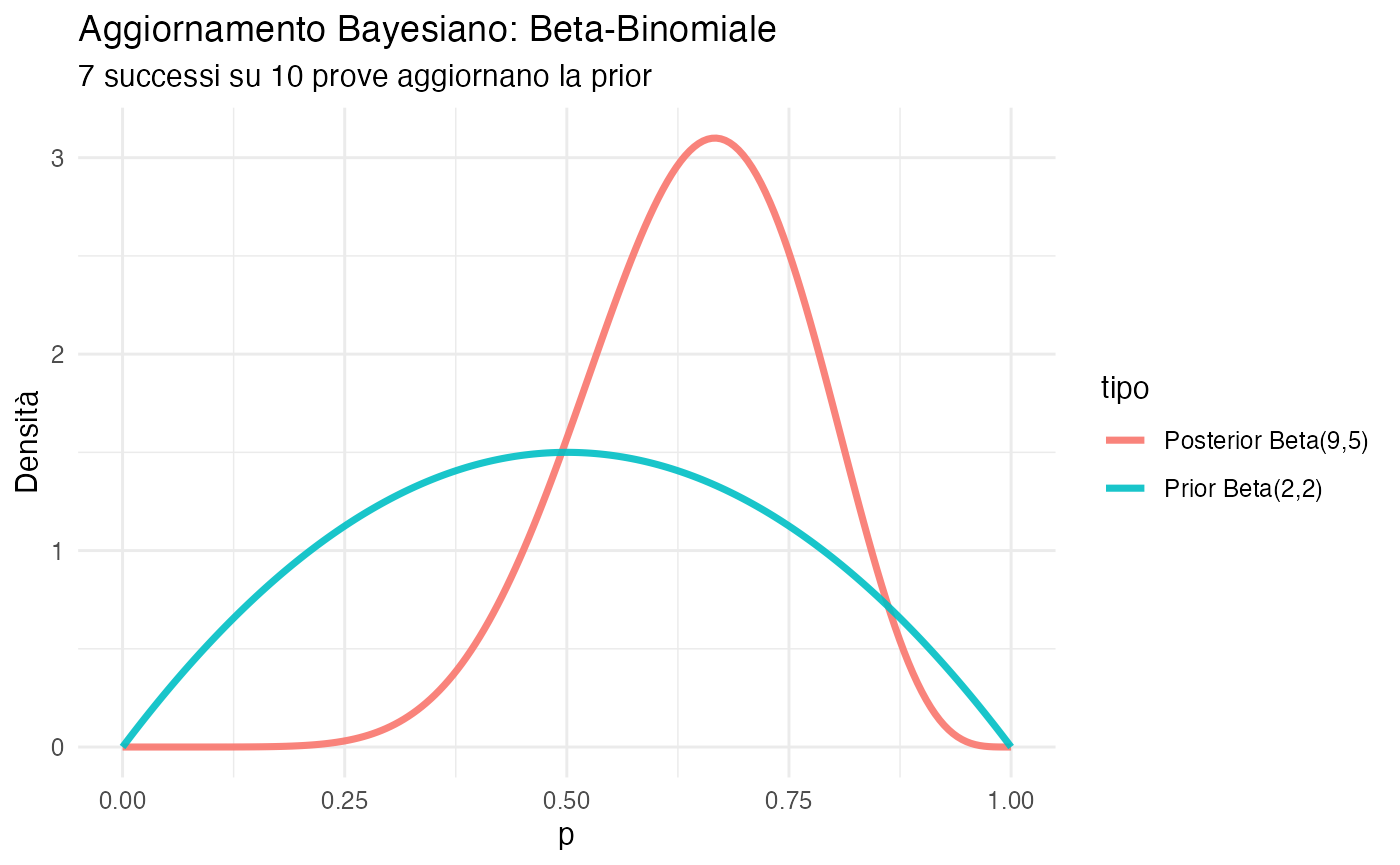
\includegraphics[width=0.85\linewidth,height=\textheight,keepaspectratio]{chapters/probability/13_cont_rv_distr_files/figure-pdf/unnamed-chunk-11-1.png}
\end{center}

\begin{Shaded}
\begin{Highlighting}[]

\FunctionTok{cat}\NormalTok{(}\StringTok{"Media prior:"}\NormalTok{, }\FunctionTok{round}\NormalTok{(alpha\_prior}\SpecialCharTok{/}\NormalTok{(alpha\_prior }\SpecialCharTok{+}\NormalTok{ beta\_prior), }\DecValTok{3}\NormalTok{), }\StringTok{"}\SpecialCharTok{\textbackslash{}n}\StringTok{"}\NormalTok{)}
\CommentTok{\#\textgreater{} Media prior: 0.5}
\FunctionTok{cat}\NormalTok{(}\StringTok{"Media posterior:"}\NormalTok{, }\FunctionTok{round}\NormalTok{(alpha\_post}\SpecialCharTok{/}\NormalTok{(alpha\_post }\SpecialCharTok{+}\NormalTok{ beta\_post), }\DecValTok{3}\NormalTok{), }\StringTok{"}\SpecialCharTok{\textbackslash{}n}\StringTok{"}\NormalTok{)}
\CommentTok{\#\textgreater{} Media posterior: 0.643}
\end{Highlighting}
\end{Shaded}

\section{Distribuzione di Cauchy}\label{distribuzione-di-cauchy}

\subsection{Definizione e interpretazione
epistemica}\label{definizione-e-interpretazione-epistemica-11}

La distribuzione di Cauchy costituisce un caso particolare della
distribuzione t di Student, corrispondente a un singolo grado di libertà
(\(t_1\)). La sua caratteristica distintiva è data dalla presenza di
code estremamente pesanti che decadono molto più lentamente rispetto a
quelle della distribuzione normale.

\begin{definition}[]\protect\hypertarget{def-cauchy}{}\label{def-cauchy}

Una variabile casuale \(X\) segue una distribuzione di Cauchy con
parametro di posizione \(\alpha\) e parametro di scala \(\beta > 0\) se
la sua funzione di densità è data da:

\[
X \sim \text{Cauchy}(\alpha, \beta), \quad f(x) = \frac{1}{\pi\beta\left[1 + \left(\frac{x-\alpha}{\beta}\right)^2\right]}
\]

\textbf{Proprietà distintive}: a differenza di molte distribuzioni
parametriche comuni, la distribuzione di Cauchy \textbf{non possiede
momenti primi e secondi definiti}. Questa peculiarità riflette il fatto
che le code della distribuzione sono sufficientemente pesanti da
impedire la convergenza degli integrali che definiscono la media e la
varianza.

\end{definition}

\textbf{Interpretazione epistemica}: la distribuzione di Cauchy esprime
un elevato grado di incertezza, assegnando una plausibilità non
trascurabile anche a valori molto distanti dal parametro di posizione
centrale. Risulta particolarmente appropriata nei contesti inferenziali
in cui non si intende escludere a priori la possibilità di osservare
valori estremamente divergenti dalla tendenza centrale, preservando così
un approccio epistemico cauto verso le potenziali osservazioni anomale.

\subsection{Ruolo nell'inferenza
bayesiana}\label{ruolo-nellinferenza-bayesiana-11}

La distribuzione di Cauchy trova ampia applicazione come distribuzione a
priori debolmente informativa e robusta nell'inferenza bayesiana. Viene
frequentemente impiegata come prior per i parametri di posizione: una
Cauchy(0, 2.5) rappresenta una scelta comune per i coefficienti di
regressione standardizzati, in quanto consente di non escludere i valori
estremi pur mantenendo la massa probabilistica concentrata attorno allo
zero. Per quanto riguarda i parametri di scala, la half-Cauchy, versione
troncata ai valori positivi della distribuzione, è spesso raccomandata
come prior per le deviazioni standard nei modelli gerarchici, grazie
alle sue proprietà desiderabili. La robustezza è un altro vantaggio
fondamentale: a differenza della distribuzione normale, la Cauchy non
penalizza eccessivamente i valori estremi, dimostrandosi quindi meno
sensibile alla possibile presenza di osservazioni anomale nei dati.

\subsection{Confronto con altre
distribuzioni}\label{confronto-con-altre-distribuzioni}

\begin{Shaded}
\begin{Highlighting}[]
\NormalTok{x }\OtherTok{\textless{}{-}} \FunctionTok{seq}\NormalTok{(}\SpecialCharTok{{-}}\DecValTok{5}\NormalTok{, }\DecValTok{5}\NormalTok{, }\AttributeTok{length.out =} \DecValTok{500}\NormalTok{)}

\NormalTok{df }\OtherTok{\textless{}{-}} \FunctionTok{data.frame}\NormalTok{(}
  \AttributeTok{x =} \FunctionTok{rep}\NormalTok{(x, }\DecValTok{3}\NormalTok{),}
  \AttributeTok{density =} \FunctionTok{c}\NormalTok{(}\FunctionTok{dnorm}\NormalTok{(x), }\FunctionTok{dt}\NormalTok{(x, }\AttributeTok{df =} \DecValTok{3}\NormalTok{), }\FunctionTok{dcauchy}\NormalTok{(x)),}
  \AttributeTok{distribuzione =} \FunctionTok{rep}\NormalTok{(}\FunctionTok{c}\NormalTok{(}\StringTok{"Normale(0,1)"}\NormalTok{, }\StringTok{"t (ν = 3)"}\NormalTok{, }\StringTok{"Cauchy(0,1)"}\NormalTok{), }\AttributeTok{each =} \FunctionTok{length}\NormalTok{(x))}
\NormalTok{)}

\FunctionTok{ggplot}\NormalTok{(df, }\FunctionTok{aes}\NormalTok{(}\AttributeTok{x =}\NormalTok{ x, }\AttributeTok{y =}\NormalTok{ density, }\AttributeTok{color =}\NormalTok{ distribuzione)) }\SpecialCharTok{+}
  \FunctionTok{geom\_line}\NormalTok{(}\AttributeTok{linewidth =} \DecValTok{1}\NormalTok{) }\SpecialCharTok{+}
  \FunctionTok{labs}\NormalTok{(}
    \AttributeTok{title =} \StringTok{"Confronto delle code"}\NormalTok{,}
    \AttributeTok{subtitle =} \StringTok{"La Cauchy ha le code più pesanti, seguita dalla t"}\NormalTok{,}
    \AttributeTok{x =} \StringTok{"x"}\NormalTok{, }\AttributeTok{y =} \StringTok{"Densità"}
\NormalTok{  ) }\SpecialCharTok{+}
  \FunctionTok{theme\_minimal}\NormalTok{() }\SpecialCharTok{+}
  \FunctionTok{scale\_color\_brewer}\NormalTok{(}\AttributeTok{palette =} \StringTok{"Set1"}\NormalTok{)}
\end{Highlighting}
\end{Shaded}

\begin{center}
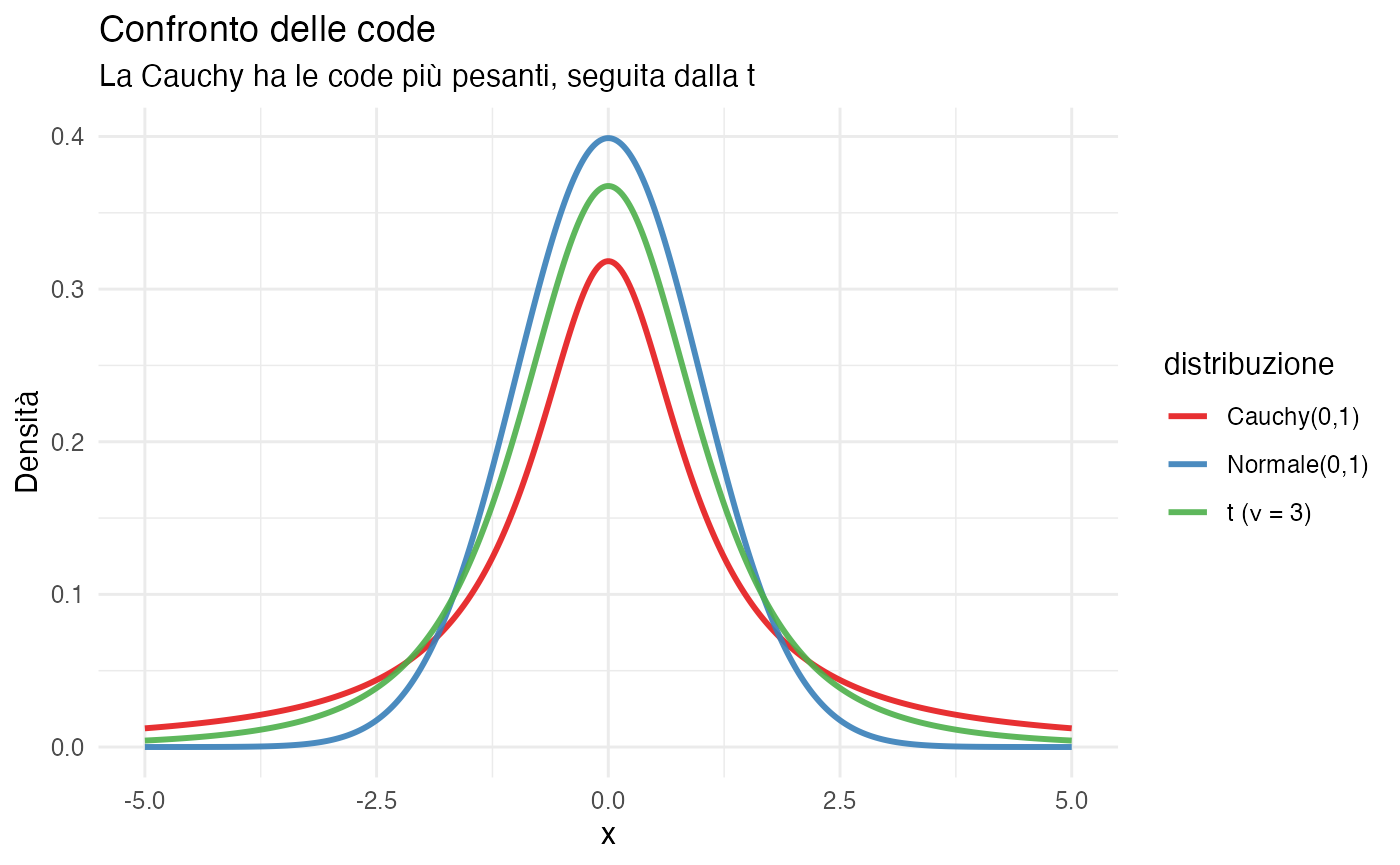
\includegraphics[width=0.85\linewidth,height=\textheight,keepaspectratio]{chapters/probability/13_cont_rv_distr_files/figure-pdf/unnamed-chunk-12-1.png}
\end{center}

\subsection{Distribuzione gamma}\label{distribuzione-gamma}

\subsubsection{Definizione e interpretazione
epistemica}\label{definizione-e-interpretazione-epistemica-12}

La distribuzione gamma rappresenta una famiglia di distribuzioni per
variabili casuali strettamente positive, che svolge un ruolo
fondamentale come distribuzione a priori coniugata per il parametro di
tasso nella distribuzione di Poisson.

\begin{definition}[]\protect\hypertarget{def-gamma}{}\label{def-gamma}

Una variabile casuale \(X\) segue una distribuzione gamma con parametro
di forma \(\alpha > 0\) e parametro di tasso \(\beta > 0\) quando la sua
funzione di densità è data da:

\[
X \sim \text{Gamma}(\alpha, \beta), \quad f(x) = \frac{\beta^\alpha x^{\alpha-1} e^{-\beta x}}{\Gamma(\alpha)} \quad \text{per } x > 0
\]

\textbf{Proprietà fondamentali}:
\(\mathbb{E}(X) = \frac{\alpha}{\beta}\),
\(\mathbb{V}(X) = \frac{\alpha}{\beta^2}\).

\end{definition}

\textbf{Interpretazione epistemica dei parametri}: Il parametro di forma
\(\alpha\) determina la configurazione morfologica della distribuzione:
quando \(\alpha < 1\) la densità risulta monotona decrescente, per
\(\alpha = 1\) si ottiene la distribuzione esponenziale, mentre per
\(\alpha > 1\) la distribuzione presenta una forma unimodale. Il
parametro di tasso \(\beta\) governa invece la scala della
distribuzione, per cui valori più elevati tendono a concentrare la massa
probabilistica in prossimità dello zero.

\subsubsection{Ruolo nell'inferenza
bayesiana}\label{ruolo-nellinferenza-bayesiana-12}

La distribuzione gamma riveste un ruolo di primo piano nell'inferenza
bayesiana grazie alle sue molteplici applicazioni. In primo luogo, funge
da distribuzione a priori coniugata per il parametro \(\lambda\) nel
modello di Poisson:

\[
\text{Prior: } \lambda \sim \text{Gamma}(\alpha, \beta), \quad \text{Dati: } y_1, \ldots, y_n \sim \text{Poisson}(\lambda)
\]

\[
\text{Posterior: } \lambda \mid \mathbf{y} \sim \text{Gamma}\left(\alpha + \sum y_i, \beta + n\right)
\]

In secondo luogo, la distribuzione gamma è comunemente utilizzata come
distribuzione a priori per il parametro di precisione (definito come
l'inverso della varianza) nei modelli normali. Infine, essa fornisce un
modello flessibile per la rappresentazione dei tempi di attesa,
generalizzando la distribuzione esponenziale al caso in cui si considera
l'attesa per il verificarsi di \(\alpha\) eventi successivi.

\subsection{Esempio: inferenza su un tasso
Poisson}\label{esempio-inferenza-su-un-tasso-poisson}

\begin{Shaded}
\begin{Highlighting}[]
\CommentTok{\# Prior: Gamma(2, 1) {-} credenza che λ sia intorno a 2}
\NormalTok{alpha\_prior }\OtherTok{\textless{}{-}} \DecValTok{2}
\NormalTok{beta\_prior }\OtherTok{\textless{}{-}} \DecValTok{1}

\CommentTok{\# Dati: 5 osservazioni con totale 18 eventi}
\NormalTok{n\_obs }\OtherTok{\textless{}{-}} \DecValTok{5}
\NormalTok{totale\_eventi }\OtherTok{\textless{}{-}} \DecValTok{18}

\CommentTok{\# Posterior: Gamma(2 + 18, 1 + 5) = Gamma(20, 6)}
\NormalTok{alpha\_post }\OtherTok{\textless{}{-}}\NormalTok{ alpha\_prior }\SpecialCharTok{+}\NormalTok{ totale\_eventi}
\NormalTok{beta\_post }\OtherTok{\textless{}{-}}\NormalTok{ beta\_prior }\SpecialCharTok{+}\NormalTok{ n\_obs}

\CommentTok{\# Visualizzazione}
\NormalTok{x }\OtherTok{\textless{}{-}} \FunctionTok{seq}\NormalTok{(}\DecValTok{0}\NormalTok{, }\DecValTok{8}\NormalTok{, }\AttributeTok{length.out =} \DecValTok{200}\NormalTok{)}
\NormalTok{df }\OtherTok{\textless{}{-}} \FunctionTok{data.frame}\NormalTok{(}
  \AttributeTok{x =} \FunctionTok{rep}\NormalTok{(x, }\DecValTok{2}\NormalTok{),}
  \AttributeTok{density =} \FunctionTok{c}\NormalTok{(}\FunctionTok{dgamma}\NormalTok{(x, alpha\_prior, beta\_prior), }\FunctionTok{dgamma}\NormalTok{(x, alpha\_post, beta\_post)),}
  \AttributeTok{tipo =} \FunctionTok{rep}\NormalTok{(}\FunctionTok{c}\NormalTok{(}\StringTok{"Prior Gamma(2,1)"}\NormalTok{, }\StringTok{"Posterior Gamma(20,6)"}\NormalTok{), }\AttributeTok{each =} \FunctionTok{length}\NormalTok{(x))}
\NormalTok{)}

\FunctionTok{ggplot}\NormalTok{(df, }\FunctionTok{aes}\NormalTok{(}\AttributeTok{x =}\NormalTok{ x, }\AttributeTok{y =}\NormalTok{ density, }\AttributeTok{color =}\NormalTok{ tipo)) }\SpecialCharTok{+}
  \FunctionTok{geom\_line}\NormalTok{(}\AttributeTok{linewidth =} \FloatTok{1.2}\NormalTok{) }\SpecialCharTok{+}
  \FunctionTok{labs}\NormalTok{(}
    \AttributeTok{title =} \StringTok{"Aggiornamento Bayesiano: Gamma{-}Poisson"}\NormalTok{,}
    \AttributeTok{subtitle =} \StringTok{"18 eventi in 5 osservazioni aggiornano la prior"}\NormalTok{,}
    \AttributeTok{x =} \StringTok{"λ"}\NormalTok{, }\AttributeTok{y =} \StringTok{"Densità"}
\NormalTok{  ) }\SpecialCharTok{+}
  \FunctionTok{theme\_minimal}\NormalTok{()}
\end{Highlighting}
\end{Shaded}

\begin{center}
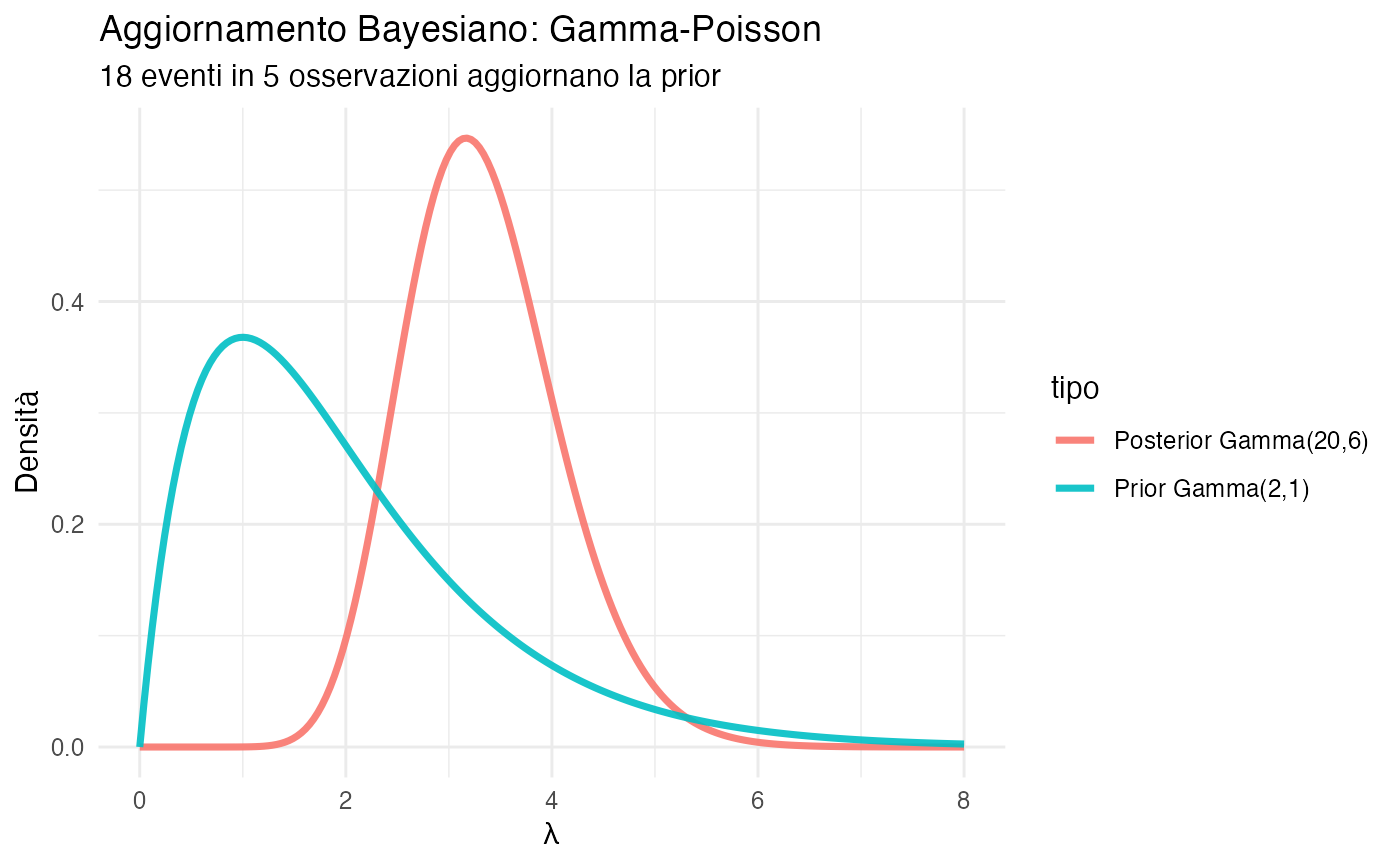
\includegraphics[width=0.85\linewidth,height=\textheight,keepaspectratio]{chapters/probability/13_cont_rv_distr_files/figure-pdf/unnamed-chunk-13-1.png}
\end{center}

\begin{Shaded}
\begin{Highlighting}[]

\FunctionTok{cat}\NormalTok{(}\StringTok{"Media prior:"}\NormalTok{, }\FunctionTok{round}\NormalTok{(alpha\_prior}\SpecialCharTok{/}\NormalTok{beta\_prior, }\DecValTok{3}\NormalTok{), }\StringTok{"}\SpecialCharTok{\textbackslash{}n}\StringTok{"}\NormalTok{)}
\CommentTok{\#\textgreater{} Media prior: 2}
\FunctionTok{cat}\NormalTok{(}\StringTok{"Media posterior:"}\NormalTok{, }\FunctionTok{round}\NormalTok{(alpha\_post}\SpecialCharTok{/}\NormalTok{beta\_post, }\DecValTok{3}\NormalTok{), }\StringTok{"}\SpecialCharTok{\textbackslash{}n}\StringTok{"}\NormalTok{)}
\CommentTok{\#\textgreater{} Media posterior: 3.33}
\FunctionTok{cat}\NormalTok{(}\StringTok{"IC 95\%: ["}\NormalTok{, }\FunctionTok{round}\NormalTok{(}\FunctionTok{qgamma}\NormalTok{(}\FloatTok{0.025}\NormalTok{, alpha\_post, beta\_post), }\DecValTok{2}\NormalTok{), }\StringTok{", "}\NormalTok{, }
    \FunctionTok{round}\NormalTok{(}\FunctionTok{qgamma}\NormalTok{(}\FloatTok{0.975}\NormalTok{, alpha\_post, beta\_post), }\DecValTok{2}\NormalTok{), }\StringTok{"]}\SpecialCharTok{\textbackslash{}n}\StringTok{"}\NormalTok{, }\AttributeTok{sep =} \StringTok{""}\NormalTok{)}
\CommentTok{\#\textgreater{} IC 95\%: [2.04, 4.95]}
\end{Highlighting}
\end{Shaded}

\subsection{Visualizzazione della
flessibilità}\label{visualizzazione-della-flessibilituxe0}

\begin{Shaded}
\begin{Highlighting}[]
\NormalTok{x }\OtherTok{\textless{}{-}} \FunctionTok{seq}\NormalTok{(}\DecValTok{0}\NormalTok{, }\DecValTok{10}\NormalTok{, }\AttributeTok{length.out =} \DecValTok{200}\NormalTok{)}
\NormalTok{params }\OtherTok{\textless{}{-}} \FunctionTok{list}\NormalTok{(}\FunctionTok{c}\NormalTok{(}\DecValTok{1}\NormalTok{, }\FloatTok{0.5}\NormalTok{), }\FunctionTok{c}\NormalTok{(}\DecValTok{2}\NormalTok{, }\FloatTok{0.5}\NormalTok{), }\FunctionTok{c}\NormalTok{(}\DecValTok{3}\NormalTok{, }\DecValTok{1}\NormalTok{), }\FunctionTok{c}\NormalTok{(}\DecValTok{5}\NormalTok{, }\DecValTok{1}\NormalTok{), }\FunctionTok{c}\NormalTok{(}\DecValTok{9}\NormalTok{, }\DecValTok{2}\NormalTok{))}

\NormalTok{df }\OtherTok{\textless{}{-}} \FunctionTok{do.call}\NormalTok{(rbind, }\FunctionTok{lapply}\NormalTok{(params, }\ControlFlowTok{function}\NormalTok{(p) \{}
  \FunctionTok{data.frame}\NormalTok{(}
    \AttributeTok{x =}\NormalTok{ x,}
    \AttributeTok{density =} \FunctionTok{dgamma}\NormalTok{(x, }\AttributeTok{shape =}\NormalTok{ p[}\DecValTok{1}\NormalTok{], }\AttributeTok{rate =}\NormalTok{ p[}\DecValTok{2}\NormalTok{]),}
    \AttributeTok{label =} \FunctionTok{paste0}\NormalTok{(}\StringTok{"α = "}\NormalTok{, p[}\DecValTok{1}\NormalTok{], }\StringTok{", β = "}\NormalTok{, p[}\DecValTok{2}\NormalTok{])}
\NormalTok{  )}
\NormalTok{\}))}

\FunctionTok{ggplot}\NormalTok{(df, }\FunctionTok{aes}\NormalTok{(}\AttributeTok{x =}\NormalTok{ x, }\AttributeTok{y =}\NormalTok{ density, }\AttributeTok{color =}\NormalTok{ label)) }\SpecialCharTok{+}
  \FunctionTok{geom\_line}\NormalTok{(}\AttributeTok{linewidth =} \DecValTok{1}\NormalTok{) }\SpecialCharTok{+}
  \FunctionTok{labs}\NormalTok{(}
    \AttributeTok{title =} \StringTok{"Flessibilità della distribuzione Gamma"}\NormalTok{,}
    \AttributeTok{x =} \StringTok{"x"}\NormalTok{, }\AttributeTok{y =} \StringTok{"f(x)"}
\NormalTok{  ) }\SpecialCharTok{+}
  \FunctionTok{theme\_minimal}\NormalTok{() }\SpecialCharTok{+}
  \FunctionTok{theme}\NormalTok{(}\AttributeTok{legend.title =} \FunctionTok{element\_blank}\NormalTok{())}
\end{Highlighting}
\end{Shaded}

\begin{center}
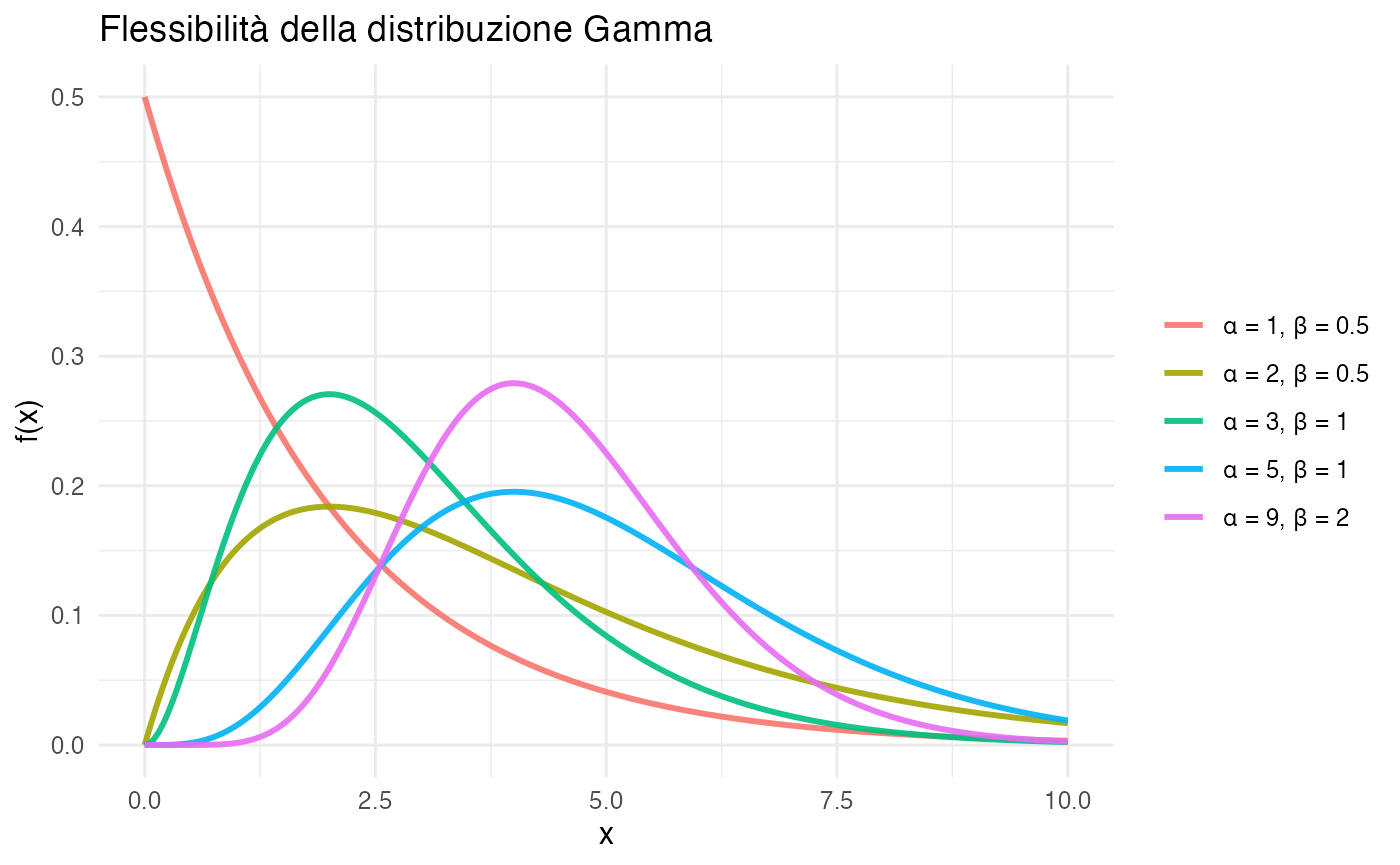
\includegraphics[width=0.85\linewidth,height=\textheight,keepaspectratio]{chapters/probability/13_cont_rv_distr_files/figure-pdf/unnamed-chunk-14-1.png}
\end{center}

\section*{Riflessioni conclusive}\label{riflessioni-conclusive-11}

\markright{Riflessioni conclusive}

Le distribuzioni continue che abbiamo esplorato costituiscono il
vocabolario fondamentale per esprimere credenze su quantità numeriche
nell'inferenza bayesiana. Ogni famiglia presenta caratteristiche
distintive che la rendono adatta a ruoli specifici.

\subsection*{Riepilogo dei ruoli nell'inferenza
bayesiana}\label{riepilogo-dei-ruoli-nellinferenza-bayesiana}

\begin{longtable}[]{@{}
  >{\raggedright\arraybackslash}p{(\linewidth - 6\tabcolsep) * \real{0.2381}}
  >{\raggedright\arraybackslash}p{(\linewidth - 6\tabcolsep) * \real{0.1429}}
  >{\raggedright\arraybackslash}p{(\linewidth - 6\tabcolsep) * \real{0.2857}}
  >{\raggedright\arraybackslash}p{(\linewidth - 6\tabcolsep) * \real{0.3333}}@{}}
\toprule\noalign{}
\begin{minipage}[b]{\linewidth}\raggedright
Distribuzione
\end{minipage} & \begin{minipage}[b]{\linewidth}\raggedright
Dominio
\end{minipage} & \begin{minipage}[b]{\linewidth}\raggedright
Ruolo principale
\end{minipage} & \begin{minipage}[b]{\linewidth}\raggedright
Prior coniugata per
\end{minipage} \\
\midrule\noalign{}
\endhead
\bottomrule\noalign{}
\endlastfoot
Uniforme & \([a, b]\) & Prior non informativa & --- \\
Esponenziale & \((0, \infty)\) & Verosimiglianza per tempi & --- \\
Normale & \(\mathbb{R}\) & Prior/verosimiglianza per medie & \(\mu\)
nella normale \\
Chi-quadrato & \((0, \infty)\) & Modellazione varianze & --- \\
t di Student & \(\mathbb{R}\) & Prior robusta, predittiva & --- \\
Beta & \((0, 1)\) & Prior per proporzioni & \(p\) nella binomiale \\
Cauchy & \(\mathbb{R}\) & Prior robusta debolmente informativa & --- \\
Gamma & \((0, \infty)\) & Prior per tassi e precisioni & \(\lambda\)
nella Poisson \\
\end{longtable}

\subsection*{Principi guida per la
scelta}\label{principi-guida-per-la-scelta}

La scelta della distribuzione appropriata dipende da tre considerazioni.
Il \textbf{dominio del parametro} è il primo vincolo: la beta è
richiesta per le proporzioni, la gamma per i tassi positivi, la normale
o la \(t\) per i parametri non vincolati. L'\textbf{informazione a
priori} determina i valori dei parametri: le prior vaghe hanno parametri
che producono distribuzioni disperse, le prior informative hanno
parametri che concentrano la massa. La \textbf{robustezza desiderata}
influenza la scelta tra distribuzioni con code diverse: la Cauchy e la
\(t\) con pochi gradi di libertà sono più robuste agli outlier della
normale.

\subsection*{La prospettiva unificante}\label{la-prospettiva-unificante}

Tutte queste distribuzioni condividono lo stesso ruolo epistemico: sono
strumenti per rappresentare formalmente i nostri gradi di credenza. Non
descrivono ``come sono realmente le cose'', ma codificano ``quanto
riteniamo plausibile ciascun valore''. Questa interpretazione
soggettivista è il filo conduttore che unisce le diverse famiglie in un
framework coerente per il ragionamento sotto incertezza.

Le proprietà matematiche, come la coniugazione, i momenti e il
comportamento delle code, non sono fini a sé stesse, ma hanno
conseguenze epistemiche: determinano come le nostre credenze si
aggiornano, quanta incertezza residua permane e quali previsioni
possiamo fare riguardo alle osservazioni future.

\begin{tcolorbox}[enhanced jigsaw, arc=.35mm, breakable, colbacktitle=quarto-callout-caution-color!10!white, opacityback=0, toprule=.15mm, rightrule=.15mm, colback=white, opacitybacktitle=0.6, leftrule=.75mm, coltitle=black, bottomtitle=1mm, left=2mm, toptitle=1mm, title=\textcolor{quarto-callout-caution-color}{\faFire}\hspace{0.5em}{Informazioni sull'ambiente di sviluppo}, titlerule=0mm, bottomrule=.15mm, colframe=quarto-callout-caution-color-frame]

\begin{Shaded}
\begin{Highlighting}[]
\FunctionTok{sessionInfo}\NormalTok{()}
\CommentTok{\#\textgreater{} R version 4.5.2 (2025{-}10{-}31)}
\CommentTok{\#\textgreater{} Platform: aarch64{-}apple{-}darwin20}
\CommentTok{\#\textgreater{} Running under: macOS Tahoe 26.1}
\CommentTok{\#\textgreater{} }
\CommentTok{\#\textgreater{} Matrix products: default}
\CommentTok{\#\textgreater{} BLAS:   /System/Library/Frameworks/Accelerate.framework/Versions/A/Frameworks/vecLib.framework/Versions/A/libBLAS.dylib }
\CommentTok{\#\textgreater{} LAPACK: /Library/Frameworks/R.framework/Versions/4.5{-}arm64/Resources/lib/libRlapack.dylib;  LAPACK version 3.12.1}
\CommentTok{\#\textgreater{} }
\CommentTok{\#\textgreater{} locale:}
\CommentTok{\#\textgreater{} [1] C.UTF{-}8/UTF{-}8/C.UTF{-}8/C/C.UTF{-}8/C.UTF{-}8}
\CommentTok{\#\textgreater{} }
\CommentTok{\#\textgreater{} time zone: Europe/Rome}
\CommentTok{\#\textgreater{} tzcode source: internal}
\CommentTok{\#\textgreater{} }
\CommentTok{\#\textgreater{} attached base packages:}
\CommentTok{\#\textgreater{} [1] stats     graphics  grDevices utils     datasets  methods   base     }
\CommentTok{\#\textgreater{} }
\CommentTok{\#\textgreater{} other attached packages:}
\CommentTok{\#\textgreater{}  [1] pillar\_1.11.1         tinytable\_0.15.1      patchwork\_1.3.2      }
\CommentTok{\#\textgreater{}  [4] ggdist\_3.3.3          tidybayes\_3.0.7       bayesplot\_1.14.0     }
\CommentTok{\#\textgreater{}  [7] ggplot2\_4.0.1         reliabilitydiag\_0.2.1 priorsense\_1.2.0     }
\CommentTok{\#\textgreater{} [10] posterior\_1.6.1       loo\_2.8.0             rstan\_2.32.7         }
\CommentTok{\#\textgreater{} [13] StanHeaders\_2.32.10   brms\_2.23.0           Rcpp\_1.1.0           }
\CommentTok{\#\textgreater{} [16] sessioninfo\_1.2.3     conflicted\_1.2.0      janitor\_2.2.1        }
\CommentTok{\#\textgreater{} [19] matrixStats\_1.5.0     modelr\_0.1.11         tibble\_3.3.0         }
\CommentTok{\#\textgreater{} [22] dplyr\_1.1.4           tidyr\_1.3.1           rio\_1.2.4            }
\CommentTok{\#\textgreater{} [25] here\_1.0.2           }
\CommentTok{\#\textgreater{} }
\CommentTok{\#\textgreater{} loaded via a namespace (and not attached):}
\CommentTok{\#\textgreater{}  [1] svUnit\_1.0.8          tidyselect\_1.2.1      farver\_2.1.2         }
\CommentTok{\#\textgreater{}  [4] S7\_0.2.1              fastmap\_1.2.0         TH.data\_1.1{-}5        }
\CommentTok{\#\textgreater{}  [7] tensorA\_0.36.2.1      digest\_0.6.39         timechange\_0.3.0     }
\CommentTok{\#\textgreater{} [10] estimability\_1.5.1    lifecycle\_1.0.4       survival\_3.8{-}3       }
\CommentTok{\#\textgreater{} [13] magrittr\_2.0.4        compiler\_4.5.2        rlang\_1.1.6          }
\CommentTok{\#\textgreater{} [16] tools\_4.5.2           knitr\_1.50            labeling\_0.4.3       }
\CommentTok{\#\textgreater{} [19] bridgesampling\_1.2{-}1  curl\_7.0.0            pkgbuild\_1.4.8       }
\CommentTok{\#\textgreater{} [22] RColorBrewer\_1.1{-}3    abind\_1.4{-}8           multcomp\_1.4{-}29      }
\CommentTok{\#\textgreater{} [25] withr\_3.0.2           purrr\_1.2.0           grid\_4.5.2           }
\CommentTok{\#\textgreater{} [28] stats4\_4.5.2          colorspace\_2.1{-}2      xtable\_1.8{-}4         }
\CommentTok{\#\textgreater{} [31] inline\_0.3.21         emmeans\_2.0.0         scales\_1.4.0         }
\CommentTok{\#\textgreater{} [34] MASS\_7.3{-}65           cli\_3.6.5             mvtnorm\_1.3{-}3        }
\CommentTok{\#\textgreater{} [37] rmarkdown\_2.30        ragg\_1.5.0            generics\_0.1.4       }
\CommentTok{\#\textgreater{} [40] RcppParallel\_5.1.11{-}1 cachem\_1.1.0          stringr\_1.6.0        }
\CommentTok{\#\textgreater{} [43] splines\_4.5.2         parallel\_4.5.2        vctrs\_0.6.5          }
\CommentTok{\#\textgreater{} [46] V8\_8.0.1              Matrix\_1.7{-}4          sandwich\_3.1{-}1       }
\CommentTok{\#\textgreater{} [49] jsonlite\_2.0.0        arrayhelpers\_1.1{-}0    systemfonts\_1.3.1    }
\CommentTok{\#\textgreater{} [52] glue\_1.8.0            codetools\_0.2{-}20      distributional\_0.5.0 }
\CommentTok{\#\textgreater{} [55] lubridate\_1.9.4       stringi\_1.8.7         gtable\_0.3.6         }
\CommentTok{\#\textgreater{} [58] QuickJSR\_1.8.1        htmltools\_0.5.8.1     Brobdingnag\_1.2{-}9    }
\CommentTok{\#\textgreater{} [61] R6\_2.6.1              textshaping\_1.0.4     rprojroot\_2.1.1      }
\CommentTok{\#\textgreater{} [64] evaluate\_1.0.5        lattice\_0.22{-}7        backports\_1.5.0      }
\CommentTok{\#\textgreater{} [67] memoise\_2.0.1         broom\_1.0.10          snakecase\_0.11.1     }
\CommentTok{\#\textgreater{} [70] rstantools\_2.5.0      coda\_0.19{-}4.1         gridExtra\_2.3        }
\CommentTok{\#\textgreater{} [73] nlme\_3.1{-}168          checkmate\_2.3.3       xfun\_0.54            }
\CommentTok{\#\textgreater{} [76] zoo\_1.8{-}14            pkgconfig\_2.0.3}
\end{Highlighting}
\end{Shaded}

\end{tcolorbox}

\section*{Bibliografia}\label{bibliografia-9}
\addcontentsline{toc}{section}{Bibliografia}

\markright{Bibliografia}

\chapter{La verosimiglianza}\label{sec-prob-likelihood}

\section*{Introduzione}\label{introduzione-13}

\markright{Introduzione}

Nei capitoli precedenti abbiamo studiato le distribuzioni di probabilità
come strumenti per descrivere il comportamento delle variabili casuali.
Abbiamo visto come, una volta assunto un modello probabilistico con
parametri noti, sia possibile calcolare la probabilità di osservare
specifici valori o configurazioni di dati.

Nella pratica della ricerca scientifica, tuttavia, ci si trova di fronte
al problema inverso. Si raccoglie un insieme di dati osservati e ci si
chiede quali siano i valori dei parametri più plausibili o compatibili
con quell'evidenza empirica. È proprio questo ribaltamento di
prospettiva, dal calcolo della probabilità dei dati in base al modello
alla stima dei parametri del modello in base ai dati, a costituire il
cuore dell'inferenza statistica.

La funzione di verosimiglianza fornisce una risposta a questo problema
inverso. Essa quantifica la plausibilità dei dati osservati per ciascuno
dei possibili valori dei parametri, a condizione che il modello sia
corretto. In pratica, la funzione di verosimiglianza costruisce una
mappa della \emph{plausibilità parametrica} che consente di individuare
i valori dei parametri che meglio spiegano i dati osservati.

In questo capitolo, la funzione di verosimiglianza viene introdotta come
concetto fondamentale per l'inferenza bayesiana. Nel capitolo successivo
esploreremo le sue proprietà matematiche e mostreremo come essa dia
origine alla distribuzione a posteriori quando viene combinata con le
nostre credenze a priori.

\subsection*{Panoramica del capitolo}\label{panoramica-del-capitolo-9}

\begin{itemize}
\tightlist
\item
  Definizione e interpretazione della funzione di verosimiglianza.
\item
  Distinzione tra verosimiglianza e funzione di probabilità.
\item
  Log-verosimiglianza: vantaggi computazionali e analitici.
\item
  Verosimiglianza per dati binomiali e gaussiani.
\item
  Stima di massima verosimiglianza (MLE).
\item
  Verosimiglianza congiunta per osservazioni multiple.
\item
  Rapporto di verosimiglianze per il confronto tra ipotesi.
\end{itemize}

\begin{tcolorbox}[enhanced jigsaw, arc=.35mm, breakable, colbacktitle=quarto-callout-tip-color!10!white, opacityback=0, toprule=.15mm, rightrule=.15mm, colback=white, opacitybacktitle=0.6, leftrule=.75mm, coltitle=black, bottomtitle=1mm, left=2mm, toptitle=1mm, title=\textcolor{quarto-callout-tip-color}{\faLightbulb}\hspace{0.5em}{Prerequisiti}, titlerule=0mm, bottomrule=.15mm, colframe=quarto-callout-tip-color-frame]

\begin{itemize}
\tightlist
\item
  Capitoli sulle distribuzioni di variabili casuali discrete e continue.
\item
  Familiarità con la distribuzione binomiale e normale.
\end{itemize}

\end{tcolorbox}

\begin{tcolorbox}[enhanced jigsaw, arc=.35mm, breakable, colbacktitle=quarto-callout-caution-color!10!white, opacityback=0, toprule=.15mm, rightrule=.15mm, colback=white, opacitybacktitle=0.6, leftrule=.75mm, coltitle=black, bottomtitle=1mm, left=2mm, toptitle=1mm, title=\textcolor{quarto-callout-caution-color}{\faFire}\hspace{0.5em}{Preparazione del Notebook}, titlerule=0mm, bottomrule=.15mm, colframe=quarto-callout-caution-color-frame]

\begin{Shaded}
\begin{Highlighting}[]
\NormalTok{here}\SpecialCharTok{::}\FunctionTok{here}\NormalTok{(}\StringTok{"code"}\NormalTok{, }\StringTok{"\_common.R"}\NormalTok{) }\SpecialCharTok{|\textgreater{}} 
  \FunctionTok{source}\NormalTok{()}
\end{Highlighting}
\end{Shaded}

\end{tcolorbox}

\section{Il principio della
verosimiglianza}\label{il-principio-della-verosimiglianza}

\subsection{Definizione formale}\label{definizione-formale-1}

Il principio di verosimiglianza costituisce uno dei fondamenti
dell'inferenza statistica, fornendo un criterio rigoroso per valutare la
plausibilità di ciascun valore possibile dei parametri alla luce dei
dati osservati.

\begin{definition}[Funzione di
verosimiglianza]\protect\hypertarget{def-likelihood}{}\label{def-likelihood}

Sia \(Y\) una variabile (o vettore) casuale la cui distribuzione dipende
da un parametro incognito \(\theta \in \Theta\). La distribuzione è
descritta da una funzione di densità (per variabili continue) o di massa
(per variabili discrete), indicata con \(f(y \mid \theta)\).

Dopo aver osservato i dati \(y\), la \emph{funzione di verosimiglianza}
per \(\theta\) è definita come: \[
L(\theta; y) = f(y \mid \theta).
\]

In questa formulazione:

\begin{itemize}
\tightlist
\item
  \(y\) è \textbf{fissato}: rappresenta i dati effettivamente osservati;
\item
  \(\theta\) è \textbf{variabile}: rappresenta i valori possibili
  \(\theta \in \Theta\) del parametro incognito oggetto di inferenza.
\end{itemize}

Pertanto, \(L(\theta; y)\) assegna a ciascun possibile valore di
\(\theta\) un grado di coerenza con l'evidenza empirica.

\end{definition}

\textbf{Interpretazione:} la verosimiglianza \textbf{non} è la
probabilità che un'ipotesi su \(\theta\) sia vera. Piuttosto, essa
quantifica la plausibilità dei dati osservati \emph{supponendo vero}
ciascuno dei possibili valori del parametro. I valori di \(\theta\) che
rendono i dati più plausibili ricevono un supporto maggiore dalla
verosimiglianza.

\subsection{Verosimiglianza e funzione di probabilità: due
prospettive}\label{verosimiglianza-e-funzione-di-probabilituxe0-due-prospettive}

Sebbene abbiano la stessa forma matematica \(f(y \mid \theta)\), la
funzione di probabilità e la funzione di verosimiglianza differiscono
radicalmente nel ruolo che assegnano ai dati \(y\) e al parametro
\(\theta\).

\begin{itemize}
\tightlist
\item
  \textbf{La funzione di probabilità} descrive la distribuzione dei dati
  \emph{prima} che essi siano stati osservati. Risponde alla domanda:
  ``Se il parametro fosse \(\theta\), quanto sarebbero probabili i
  possibili esiti \(y\)?''. In questo caso, \(\theta\) è \textbf{fisso}
  (un'ipotesi) e \(y\) è \textbf{variabile} (l'esito incerto).
\item
  \textbf{La funzione di verosimiglianza}, invece, valuta la
  plausibilità dei parametri \emph{dopo} aver osservato i dati. Risponde
  alla domanda: ``Avendo osservato il dato \(y\), quanto sono plausibili
  i possibili valori di \(\theta\)?''. In questo caso, \(y\) è
  \textbf{fisso} (l'evidenza) e \(\theta\) è \textbf{variabile}
  (l'oggetto dell'inferenza).
\end{itemize}

In sintesi, il passaggio dalla probabilità alla verosimiglianza
corrisponde a un cambio di prospettiva: dai dati \emph{potenziali} al
parametro \emph{incognito}.

\begin{longtable}[]{@{}
  >{\raggedright\arraybackslash}p{(\linewidth - 4\tabcolsep) * \real{0.2319}}
  >{\raggedright\arraybackslash}p{(\linewidth - 4\tabcolsep) * \real{0.3623}}
  >{\raggedright\arraybackslash}p{(\linewidth - 4\tabcolsep) * \real{0.4058}}@{}}
\toprule\noalign{}
\begin{minipage}[b]{\linewidth}\raggedright
Caratteristica
\end{minipage} & \begin{minipage}[b]{\linewidth}\raggedright
Funzione di probabilità
\end{minipage} & \begin{minipage}[b]{\linewidth}\raggedright
Funzione di verosimiglianza
\end{minipage} \\
\midrule\noalign{}
\endhead
\bottomrule\noalign{}
\endlastfoot
Variabile & \(y\) (aleatoria) & \(\theta\) (incognita) \\
Costante & \(\theta\) (noto) & \(y\) (osservato) \\
Domanda & Quali dati aspettarsi? & Quali valori dei parametri sono più
plausibili? \\
Uso & Predizione & Inferenza \\
\end{longtable}

Questa dualità riflette un principio fondamentale: la stessa formula
matematica assume significati distinti a seconda che l'obiettivo sia la
predizione o l'inferenza.

\begin{tcolorbox}[enhanced jigsaw, arc=.35mm, breakable, colbacktitle=quarto-callout-important-color!10!white, opacityback=0, toprule=.15mm, rightrule=.15mm, colback=white, opacitybacktitle=0.6, leftrule=.75mm, coltitle=black, bottomtitle=1mm, left=2mm, toptitle=1mm, title=\textcolor{quarto-callout-important-color}{\faExclamation}\hspace{0.5em}{Il ruolo della verosimiglianza nell'inferenza bayesiana}, titlerule=0mm, bottomrule=.15mm, colframe=quarto-callout-important-color-frame]

Nell'approccio bayesiano, la verosimiglianza funge da \textbf{ponte} tra
i dati e i parametri. Essa si combina con la distribuzione a priori per
produrre la distribuzione a posteriori: \[
p(\theta \mid y) \propto L(\theta; y) \cdot p(\theta).
\]

I dati aggiornano le credenze su \(\theta\) \textbf{attraverso} la
verosimiglianza. Nel prossimo capitolo esploreremo in dettaglio questo
meccanismo di aggiornamento.

\end{tcolorbox}

\section{La log-verosimiglianza}\label{la-log-verosimiglianza}

\subsection{Definizione e
motivazione}\label{definizione-e-motivazione-1}

In ambito statistico e computazionale, è spesso vantaggioso lavorare con
la \emph{log-verosimiglianza}, definita come: \[
\ell(\theta; y) = \log L(\theta; y) = \log f(y \mid \theta).
\]

Questa trasformazione offre notevoli vantaggi sia dal punto di vista
computazionale che analitico.

\subsection{Vantaggi computazionali e
analitici}\label{vantaggi-computazionali-e-analitici}

\subsubsection{Vantaggi computazionali: la stabilità
numerica}\label{vantaggi-computazionali-la-stabilituxe0-numerica}

Quando si lavora con grandi campioni, il calcolo diretto della
verosimiglianza come prodotto di molte probabilità può generare valori
numericamente indistinguibili da zero a causa dell'\emph{underflow}.
Questo problema può essere risolto trasformando il prodotto in una somma
tramite la \textbf{log-verosimiglianza}:

Per osservazioni indipendenti \(y_1, \ldots, y_n\): \[
\ell(\theta; y_1, \ldots, y_n) = \log L(\theta; y) = \sum_{i=1}^n \log f(y_i \mid \theta)
\]

Questa trasformazione garantisce stabilità numerica, in quanto le somme
sono molto meno soggette a underflow rispetto ai prodotti di valori
prossimi a zero.

\begin{tcolorbox}[enhanced jigsaw, arc=.35mm, breakable, colbacktitle=quarto-callout-caution-color!10!white, opacityback=0, toprule=.15mm, rightrule=.15mm, colback=white, opacitybacktitle=0.6, leftrule=.75mm, coltitle=black, bottomtitle=1mm, left=2mm, toptitle=1mm, title=\textcolor{quarto-callout-caution-color}{\faFire}\hspace{0.5em}{Esempio pratico: underflow vs.~stabilità}, titlerule=0mm, bottomrule=.15mm, colframe=quarto-callout-caution-color-frame]

\begin{Shaded}
\begin{Highlighting}[]
\CommentTok{\# Il prodotto diretto di molte probabilità piccole può collassare a zero (underflow)}
\NormalTok{n }\OtherTok{\textless{}{-}} \DecValTok{1000}
\NormalTok{theta }\OtherTok{\textless{}{-}} \FloatTok{0.3}
\FunctionTok{set.seed}\NormalTok{(}\DecValTok{42}\NormalTok{)}
\NormalTok{dati }\OtherTok{\textless{}{-}} \FunctionTok{sample}\NormalTok{(}\DecValTok{0}\SpecialCharTok{:}\DecValTok{1}\NormalTok{, n, }\AttributeTok{replace =} \ConstantTok{TRUE}\NormalTok{)}

\CommentTok{\# Verosimiglianza diretta: prodotto rischioso}
\FunctionTok{prod}\NormalTok{(}\FunctionTok{dbinom}\NormalTok{(dati, }\DecValTok{1}\NormalTok{, theta))  }\CommentTok{\# Potrebbe risultare 0}
\CommentTok{\#\textgreater{} [1] 0}

\CommentTok{\# Log{-}verosimiglianza: calcolo stabile}
\FunctionTok{sum}\NormalTok{(}\FunctionTok{dbinom}\NormalTok{(dati, }\DecValTok{1}\NormalTok{, theta, }\AttributeTok{log =} \ConstantTok{TRUE}\NormalTok{))  }\CommentTok{\# Restituisce un valore finito}
\CommentTok{\#\textgreater{} [1] {-}781}
\end{Highlighting}
\end{Shaded}

\end{tcolorbox}

\subsubsection{Vantaggi analitici: l'ottimizzazione
semplificata}\label{vantaggi-analitici-lottimizzazione-semplificata}

La forma della log-verosimiglianza offre anche notevoli vantaggi
analitici:

\begin{enumerate}
\def\labelenumi{\arabic{enumi}.}
\tightlist
\item
  \textbf{derivate più semplici:} le derivate di una somma sono più
  immediate da calcolare rispetto a quelle di un prodotto, il che
  semplifica notevolmente la ricerca del massimo della funzione.
\item
  \textbf{equivalenza del massimo:} poiché il logaritmo naturale è una
  funzione \textbf{monotona crescente}, massimizzare la
  log-verosimiglianza \(\ell(\theta; y)\) è matematicamente equivalente
  a massimizzare la verosimiglianza \(L(\theta; y)\). Il valore di
  \(\theta\) che massimizza l'una è dunque lo stesso che massimizza
  l'altra.
\end{enumerate}

In sintesi, l'uso della log-verosimiglianza offre un vantaggio pratico
essenziale (evitare l'underflow) e uno teorico (la semplificazione delle
procedure di ottimizzazione), rendendola uno strumento ideale per
l'inferenza statistica moderna.

\section{Verosimiglianza per dati
binomiali}\label{verosimiglianza-per-dati-binomiali}

\subsection{Un esempio introduttivo: il lancio di una
moneta}\label{un-esempio-introduttivo-il-lancio-di-una-moneta}

Consideriamo il problema di stimare la probabilità \(\theta\) che una
moneta produca \emph{Testa}. Assumiamo che ogni lancio sia indipendente
e che \(\theta\) rimanga costante.

Se in \(n\) lanci osserviamo \(y\) esiti \emph{Testa}, la probabilità
dei dati è: \[
P(\text{dati} \mid \theta) = \theta^y (1-\theta)^{n-y}.
\]

La funzione di verosimiglianza è la stessa espressione, però vista come
funzione di \(\theta\): \[
L(\theta \mid \text{dati}) \propto \theta^y (1-\theta)^{n-y}.
\]

\subsection{Esempio: due scenari a
confronto}\label{esempio-due-scenari-a-confronto}

\textbf{Scenario 1}: supponiamo di osservare un esito \emph{Testa} in
due lanci della moneta (\(n=2, y=1\)).

\begin{itemize}
\tightlist
\item
  Se \(\theta = 0.5\): \(L(0.5) = 0.5^1 \cdot 0.5^1 = 0.25.\)
\item
  Se \(\theta = 0.4\): \(L(0.4) = 0.4^1 \cdot 0.6^1 = 0.24.\)
\end{itemize}

In questo caso \(\theta=0.5\) spiega leggermente meglio i dati.

\textbf{Scenario 2}: supponiamo di osservare un esito \emph{Testa} in
tre lanci della moneta (\(n=3, y=1\)).

\begin{itemize}
\tightlist
\item
  Se \(\theta = 0.5\): \(L(0.5) = 0.5^1 \cdot 0.5^2 = 0.125\).
\item
  Se \(\theta = 0.4\): \(L(0.4) = 0.4^1 \cdot 0.6^2 = 0.144\).
\end{itemize}

Ora \(\theta = 0.4\) è più plausibile di \(\theta = 0.5\).

Con R possiamo calcolare la verosimiglianza per tutta la gamma dei
possibili valori di \(\theta\).

\begin{Shaded}
\begin{Highlighting}[]
\NormalTok{theta\_seq }\OtherTok{\textless{}{-}} \FunctionTok{seq}\NormalTok{(}\DecValTok{0}\NormalTok{, }\DecValTok{1}\NormalTok{, }\AttributeTok{length.out =} \DecValTok{200}\NormalTok{)}

\CommentTok{\# Scenario 1: 2 lanci, 1 testa}
\NormalTok{lik1 }\OtherTok{\textless{}{-}}\NormalTok{ theta\_seq}\SpecialCharTok{\^{}}\DecValTok{1} \SpecialCharTok{*}\NormalTok{ (}\DecValTok{1} \SpecialCharTok{{-}}\NormalTok{ theta\_seq)}\SpecialCharTok{\^{}}\DecValTok{1}

\CommentTok{\# Scenario 2: 3 lanci, 1 testa  }
\NormalTok{lik2 }\OtherTok{\textless{}{-}}\NormalTok{ theta\_seq}\SpecialCharTok{\^{}}\DecValTok{1} \SpecialCharTok{*}\NormalTok{ (}\DecValTok{1} \SpecialCharTok{{-}}\NormalTok{ theta\_seq)}\SpecialCharTok{\^{}}\DecValTok{2}

\NormalTok{df }\OtherTok{\textless{}{-}} \FunctionTok{data.frame}\NormalTok{(}
  \AttributeTok{theta =} \FunctionTok{rep}\NormalTok{(theta\_seq, }\DecValTok{2}\NormalTok{),}
  \AttributeTok{likelihood =} \FunctionTok{c}\NormalTok{(lik1, lik2),}
  \AttributeTok{scenario =} \FunctionTok{rep}\NormalTok{(}\FunctionTok{c}\NormalTok{(}\StringTok{"2 lanci (1 testa)"}\NormalTok{, }\StringTok{"3 lanci (1 testa)"}\NormalTok{), }\AttributeTok{each =} \FunctionTok{length}\NormalTok{(theta\_seq))}
\NormalTok{)}

\FunctionTok{ggplot}\NormalTok{(df, }\FunctionTok{aes}\NormalTok{(}\AttributeTok{x =}\NormalTok{ theta, }\AttributeTok{y =}\NormalTok{ likelihood, }\AttributeTok{color =}\NormalTok{ scenario)) }\SpecialCharTok{+}
  \FunctionTok{geom\_line}\NormalTok{(}\AttributeTok{linewidth =} \FloatTok{1.2}\NormalTok{) }\SpecialCharTok{+}
  \FunctionTok{labs}\NormalTok{(}
    \AttributeTok{x =} \FunctionTok{expression}\NormalTok{(theta),}
    \AttributeTok{y =} \StringTok{"Verosimiglianza"}\NormalTok{,}
    \AttributeTok{color =} \StringTok{"Scenario"}
\NormalTok{  ) }\SpecialCharTok{+}
  \FunctionTok{scale\_color\_manual}\NormalTok{(}\AttributeTok{values =} \FunctionTok{c}\NormalTok{(}\StringTok{"\#4E79A7"}\NormalTok{, }\StringTok{"\#E69F00"}\NormalTok{)) }\SpecialCharTok{+}
  \FunctionTok{theme\_minimal}\NormalTok{() }
\end{Highlighting}
\end{Shaded}

\begin{figure}[H]

\centering{

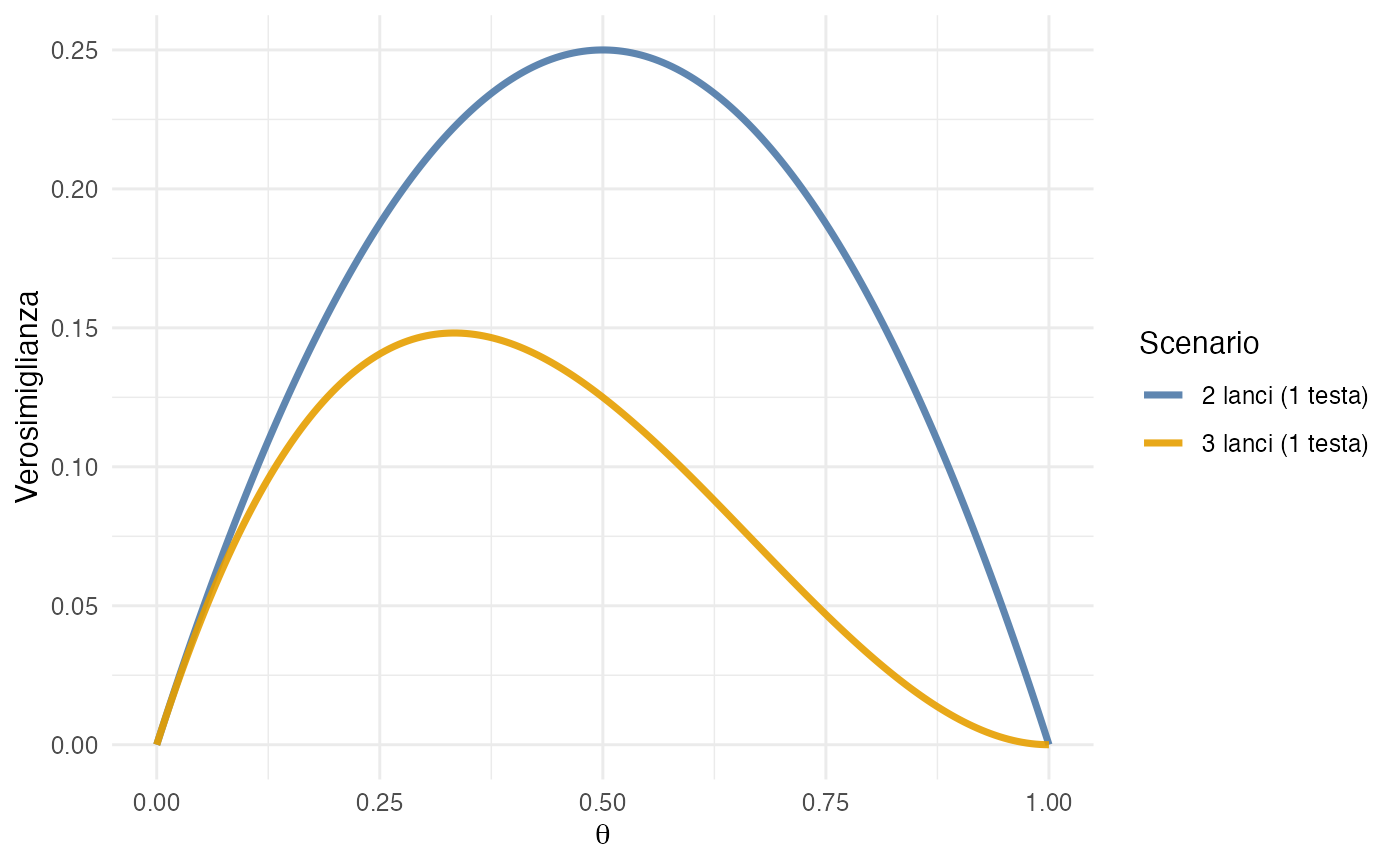
\includegraphics[width=0.85\linewidth,height=\textheight,keepaspectratio]{chapters/probability/14_likelihood_files/figure-pdf/fig-lik-comparison-1.png}

}

\caption{\label{fig-lik-comparison}Confronto delle funzioni di
verosimiglianza per due scenari. Con più dati (3 lanci), la curva è più
stretta, indicando maggiore precisione nella stima.}

\end{figure}%

\textbf{Osservazioni chiave.} Il massimo della verosimiglianza coincide
con la proporzione campionaria osservata, ossia \(\hat{\theta} = y/n\).
Inoltre, con l'aumentare della dimensione del campione, la curva di
verosimiglianza tende a concentrarsi attorno al valore massimo,
diventando progressivamente più stretta e indicando una stima più
precisa. Infine, se nel campione sono presenti sia esiti \emph{Testa}
che \emph{Croce}, i valori estremi del parametro (\(\theta\) prossimo a
0 o a 1) ricevono un supporto empirico pressoché nullo, in quanto
risulterebbero altamente incompatibili con i dati osservati.

\subsection{Verosimiglianza binomiale
completa}\label{verosimiglianza-binomiale-completa}

Consideriamo ora un esperimento con \(n = 30\) prove e \(y = 23\) eventi
\emph{Testa}. Per modellare il numero totale di eventi \emph{Testa}
utilizziamo la distribuzione binomiale, che descrive la probabilità di
ottenere esattamente \(y\) successi in \(n\) prove indipendenti, con
probabilità di successo costante, pari a \(\theta\). La funzione di
verosimiglianza si ottiene trattando la formula della distribuzione
binomiale come funzione di \(\theta\) anziché di \(y\):

\[
L(\theta \mid y, n) = \binom{n}{y} \theta^y (1-\theta)^{n-y} = \binom{30}{23} \theta^{23} (1 - \theta)^7.
\]

La funzione di verosimiglianza quantifica la plausibilità di ciascun
valore di \(\theta\) alla luce dei dati osservati. A differenza degli
esempi precedenti, in questo caso manteniamo la costante moltiplicativa
\(\binom{30}{23}\) poiché lavoreriamo con la verosimiglianza completa.

Il codice seguente genera il grafico della funzione di verosimiglianza
calcolando, per ogni valore \(\theta\), la plausibilità di osservare 23
esiti \emph{Testa} in 30 prove:

\begin{Shaded}
\begin{Highlighting}[]
\NormalTok{n }\OtherTok{\textless{}{-}} \DecValTok{30}
\NormalTok{y }\OtherTok{\textless{}{-}} \DecValTok{23}
\NormalTok{theta }\OtherTok{\textless{}{-}} \FunctionTok{seq}\NormalTok{(}\DecValTok{0}\NormalTok{, }\DecValTok{1}\NormalTok{, }\AttributeTok{length.out =} \DecValTok{1000}\NormalTok{)}
\NormalTok{likelihood }\OtherTok{\textless{}{-}} \FunctionTok{dbinom}\NormalTok{(y, }\AttributeTok{size =}\NormalTok{ n, }\AttributeTok{prob =}\NormalTok{ theta)}

\FunctionTok{ggplot}\NormalTok{(}\FunctionTok{data.frame}\NormalTok{(theta, likelihood), }\FunctionTok{aes}\NormalTok{(}\AttributeTok{x =}\NormalTok{ theta, }\AttributeTok{y =}\NormalTok{ likelihood)) }\SpecialCharTok{+}
  \FunctionTok{geom\_line}\NormalTok{(}\AttributeTok{linewidth =} \FloatTok{1.2}\NormalTok{, }\AttributeTok{color =} \StringTok{"\#4E79A7"}\NormalTok{) }\SpecialCharTok{+}
  \FunctionTok{geom\_vline}\NormalTok{(}\AttributeTok{xintercept =}\NormalTok{ y}\SpecialCharTok{/}\NormalTok{n, }\AttributeTok{linetype =} \StringTok{"dashed"}\NormalTok{, }\AttributeTok{color =} \StringTok{"\#E15759"}\NormalTok{) }\SpecialCharTok{+}
  \FunctionTok{annotate}\NormalTok{(}\StringTok{"text"}\NormalTok{, }\AttributeTok{x =}\NormalTok{ y}\SpecialCharTok{/}\NormalTok{n }\SpecialCharTok{{-}} \FloatTok{0.08}\NormalTok{, }\AttributeTok{y =} \FunctionTok{max}\NormalTok{(likelihood) }\SpecialCharTok{*} \FloatTok{0.15}\NormalTok{,}
           \AttributeTok{label =} \FunctionTok{paste0}\NormalTok{(}\StringTok{"MLE = "}\NormalTok{, }\FunctionTok{round}\NormalTok{(y}\SpecialCharTok{/}\NormalTok{n, }\DecValTok{3}\NormalTok{)), }\AttributeTok{color =} \StringTok{"\#E15759"}\NormalTok{) }\SpecialCharTok{+}
  \FunctionTok{labs}\NormalTok{(}
    \AttributeTok{x =} \FunctionTok{expression}\NormalTok{(theta),}
    \AttributeTok{y =} \StringTok{"Verosimiglianza"}
\NormalTok{  ) }\SpecialCharTok{+}
  \FunctionTok{theme\_minimal}\NormalTok{()}
\end{Highlighting}
\end{Shaded}

\begin{figure}[H]

\centering{

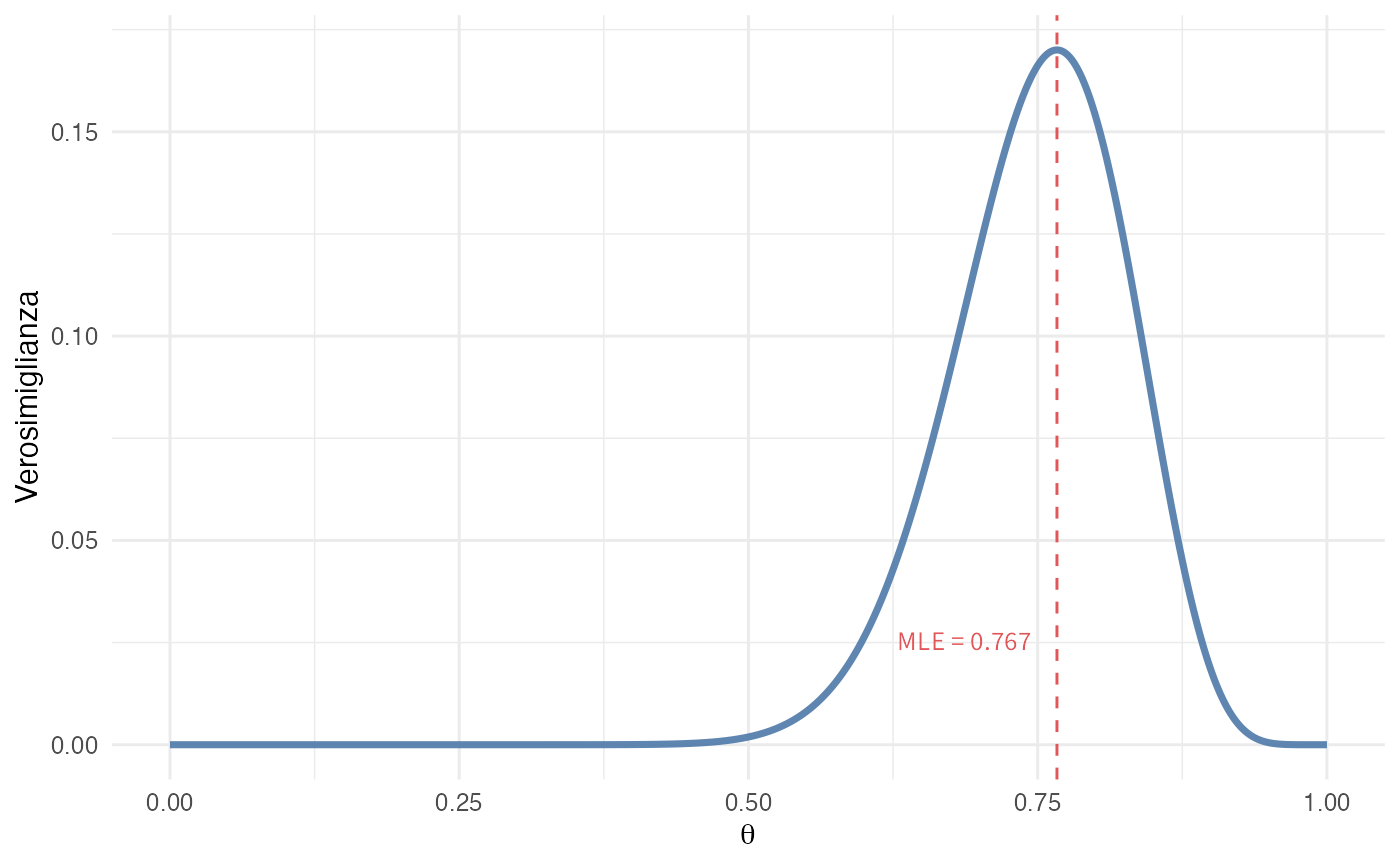
\includegraphics[width=0.85\linewidth,height=\textheight,keepaspectratio]{chapters/probability/14_likelihood_files/figure-pdf/fig-binom-lik-1.png}

}

\caption{\label{fig-binom-lik}Verosimiglianza binomiale per 23 successi
su 30 prove. Il massimo si trova in corrispondenza della proporzione
campionaria.}

\end{figure}%

L'analisi grafica della funzione di verosimiglianza rivela un profilo
caratterizzato da un picco marcato in corrispondenza di
\(\theta \approx 0.77\). Questo punto di massimo rappresenta la
\emph{stima di massima verosimiglianza} (MLE) della probabilità di
successo del processo bernoulliano in esame. Si osserva che tale stima
corrisponde esattamente alla proporzione campionaria osservata, ovvero
\(\hat{\theta}\) = 23/30.

La forma della curva di verosimiglianza mostra una dispersione limitata
attorno al valore massimo, indicando una relativa precisione della stima
ottenuta. Ciò suggerisce che il campione fornisce un'informazione
sufficientemente affidabile sul parametro della popolazione. Al
contrario, i valori estremi di \(\theta\), specialmente quelli prossimi
agli estremi 0 e 1 dell'intervallo parametrico, presentano
verosimiglianze trascurabili e sono quindi sostanzialmente incompatibili
con i dati osservati.

\section{La stima di massima
verosimiglianza}\label{la-stima-di-massima-verosimiglianza}

Quando osserviamo dei dati sperimentali e vogliamo stimare un parametro
incognito, come ad esempio, la probabilità \(\theta\) che una moneta dia
\emph{Testa}, un approccio è quello della \textbf{stima di massima
verosimiglianza} (in inglese, \emph{Maximum Likelihood Estimation},
MLE). Anche se l'inferenza bayesiana mira a ottenere la distribuzione
completa dei valori plausibili del parametro, e non un unico valore
puntuale, è utile capire in cosa consista la stima di massima
verosimiglianza.

\subsection{Il principio}\label{il-principio}

La \textbf{stima di massima verosimiglianza (MLE)} è il valore del
parametro che massimizza la funzione di verosimiglianza: \[
\hat{\theta}_{\text{MLE}} = \arg\max_{\theta} L(\theta; y).
\]

Il ragionamento alla base della MLE è semplice e intuitivo: se un certo
valore del parametro assegna ai nostri dati una probabilità (o
verosimiglianza) maggiore rispetto a ogni altra ipotesi, allora quel
valore rappresenta l'ipotesi più credibile, ovvero quella che spiega
meglio l'evidenza empirica a nostra disposizione.

\subsection{Derivazione analitica per il caso
binomiale}\label{derivazione-analitica-per-il-caso-binomiale}

Per derivare lo stimatore di massima verosimiglianza nel caso di una
prova bernoulliana ripetuta, è opportuno lavorare con la
\textbf{log-verosimiglianza}. Dati \(n\) lanci indipendenti con \(y\)
successi (\emph{Testa}), si ha:

\[
\ell(\theta) = \log L(\theta; y) = y \log \theta + (n-y) \log(1-\theta).
\]

Per trovare il massimo, calcoliamo la derivata prima rispetto a
\(\theta\) e la poniamo uguale a zero:

\[
\frac{d\ell}{d\theta} = \frac{y}{\theta} - \frac{n-y}{1-\theta} = 0.
\]

Risolvendo l'equazione per \(\theta\) si ottiene:

\[
\frac{y}{\theta} = \frac{n-y}{1-\theta} \quad \Rightarrow \quad y(1-\theta) = (n-y)\theta \quad \Rightarrow \quad y - y\theta = n\theta - y\theta \quad \Rightarrow \quad y = n\theta.
\]

Pertanto, lo stimatore di massima verosimiglianza è:

\[
\hat{\theta}_{\text{MLE}} = \frac{y}{n}.
\] In altre parole, nel modello binomiale la stima di massima
verosimiglianza per la probabilità di successo coincide con la
\textbf{proporzione campionaria} osservata.

\subsection{Implementazione in R}\label{implementazione-in-r}

La stima di massima verosimiglianza può essere implementata in R in modo
diretto, utilizzando un metodo sia esplorativo che analitico.
L'obiettivo è calcolare il valore di \(\theta\) che massimizza la
funzione di verosimiglianza o, equivalentemente, che minimizza la
log-verosimiglianza negativa.

\subsubsection{Metodo 1: ricerca su
griglia}\label{metodo-1-ricerca-su-griglia}

Questo approccio consiste nel valutare la verosimiglianza su un'ampia
griglia di valori plausibili per \(\theta\). Si tratta di un metodo
intuitivo che consente di visualizzare direttamente la funzione di
verosimiglianza.

\begin{Shaded}
\begin{Highlighting}[]
\CommentTok{\# Metodo 1: Ricerca su griglia}
\NormalTok{n }\OtherTok{\textless{}{-}} \DecValTok{30}          \CommentTok{\# Numero di lanci}
\NormalTok{y }\OtherTok{\textless{}{-}} \DecValTok{23}          \CommentTok{\# Numero di successi (Testa)}
\NormalTok{theta\_grid }\OtherTok{\textless{}{-}} \FunctionTok{seq}\NormalTok{(}\FloatTok{0.001}\NormalTok{, }\FloatTok{0.999}\NormalTok{, }\AttributeTok{length.out =} \DecValTok{10000}\NormalTok{)  }\CommentTok{\# Griglia di valori}
\NormalTok{likelihood }\OtherTok{\textless{}{-}} \FunctionTok{dbinom}\NormalTok{(y, }\AttributeTok{size =}\NormalTok{ n, }\AttributeTok{prob =}\NormalTok{ theta\_grid) }\CommentTok{\# Verosimiglianza per ogni punto}
\NormalTok{mle\_grid }\OtherTok{\textless{}{-}}\NormalTok{ theta\_grid[}\FunctionTok{which.max}\NormalTok{(likelihood)]        }\CommentTok{\# Valore che massimizza}
\end{Highlighting}
\end{Shaded}

\subsubsection{Metodo 2: ottimizzazione
numerica}\label{metodo-2-ottimizzazione-numerica}

Un approccio più efficiente utilizza algoritmi di ottimizzazione per
trovare direttamente il massimo della log-verosimiglianza. Per questo
modello, possiamo usare la funzione \texttt{optim()}.

\begin{Shaded}
\begin{Highlighting}[]
\CommentTok{\# Metodo 2: Ottimizzazione numerica}
\NormalTok{neg\_log\_lik }\OtherTok{\textless{}{-}} \ControlFlowTok{function}\NormalTok{(theta) \{}
  \CommentTok{\# Log{-}verosimiglianza negativa (per minimizzazione)}
  \SpecialCharTok{{-}}\NormalTok{(y }\SpecialCharTok{*} \FunctionTok{log}\NormalTok{(theta) }\SpecialCharTok{+}\NormalTok{ (n }\SpecialCharTok{{-}}\NormalTok{ y) }\SpecialCharTok{*} \FunctionTok{log}\NormalTok{(}\DecValTok{1} \SpecialCharTok{{-}}\NormalTok{ theta))}
\NormalTok{\}}

\CommentTok{\# Ottimizzazione vincolata nell\textquotesingle{}intervallo (0,1)}
\NormalTok{result }\OtherTok{\textless{}{-}} \FunctionTok{optim}\NormalTok{(}
  \AttributeTok{par =} \FloatTok{0.5}\NormalTok{,                    }\CommentTok{\# Valore iniziale}
  \AttributeTok{fn =}\NormalTok{ neg\_log\_lik,             }\CommentTok{\# Funzione da minimizzare}
  \AttributeTok{method =} \StringTok{"Brent"}\NormalTok{,             }\CommentTok{\# Algoritmo per problemi unidimensionali}
  \AttributeTok{lower =} \FloatTok{0.001}\NormalTok{,                }\CommentTok{\# Limite inferiore}
  \AttributeTok{upper =} \FloatTok{0.999}                 \CommentTok{\# Limite superiore}
\NormalTok{)}
\NormalTok{mle\_optim }\OtherTok{\textless{}{-}}\NormalTok{ result}\SpecialCharTok{$}\NormalTok{par         }\CommentTok{\# Stima MLE}
\end{Highlighting}
\end{Shaded}

Entrambi i metodi producono lo stesso risultato, che coincide con la
soluzione analitica \(\hat{\theta}_{\text{MLE}} = y/n\).

\begin{Shaded}
\begin{Highlighting}[]
\CommentTok{\# Confronto dei risultati}
\FunctionTok{cat}\NormalTok{(}\StringTok{"MLE (griglia):"}\NormalTok{, }\FunctionTok{round}\NormalTok{(mle\_grid, }\DecValTok{4}\NormalTok{), }\StringTok{"}\SpecialCharTok{\textbackslash{}n}\StringTok{"}\NormalTok{)}
\CommentTok{\#\textgreater{} MLE (griglia): 0.767}
\FunctionTok{cat}\NormalTok{(}\StringTok{"MLE (ottimizzazione):"}\NormalTok{, }\FunctionTok{round}\NormalTok{(mle\_optim, }\DecValTok{4}\NormalTok{), }\StringTok{"}\SpecialCharTok{\textbackslash{}n}\StringTok{"}\NormalTok{)}
\CommentTok{\#\textgreater{} MLE (ottimizzazione): 0.767}
\FunctionTok{cat}\NormalTok{(}\StringTok{"MLE (analitica):"}\NormalTok{, y}\SpecialCharTok{/}\NormalTok{n, }\StringTok{"}\SpecialCharTok{\textbackslash{}n}\StringTok{"}\NormalTok{)}
\CommentTok{\#\textgreater{} MLE (analitica): 0.767}
\end{Highlighting}
\end{Shaded}

Tutti e tre gli approcci convergono alla medesima stima, dimostrando
l'equivalenza tra il risultato analitico e le implementazioni numeriche.
La scelta del metodo dipende dal contesto: la griglia è utile per
visualizzare la verosimiglianza, mentre l'ottimizzazione diretta è più
efficiente per modelli complessi.

\subsection{Relazione con l'inferenza
bayesiana}\label{relazione-con-linferenza-bayesiana}

Nell'approccio bayesiano, lo stimatore di massima verosimiglianza (MLE)
assume un significato specifico: quando la distribuzione a priori scelta
per il parametro \(\theta\) è \textbf{uniforme}, la MLE coincide
esattamente con la \textbf{moda della distribuzione a posteriori}. Tale
stima è nota anche come \textbf{Maximum A Posteriori} (MAP).

Questo collegamento sarà approfondito nel prossimo capitolo, in cui
vedremo in dettaglio come la forma della funzione di verosimiglianza,
quando viene combinata con diverse scelte di distribuzioni a priori,
determini la distribuzione a posteriori e, di conseguenza, tutte le
inferenze che ne derivano.

\section{Verosimiglianza congiunta}\label{verosimiglianza-congiunta}

Il concetto di verosimiglianza si generalizza in modo naturale al caso
di osservazioni multiple, dando origine alla \textbf{verosimiglianza
congiunta}. Questo strumento consente di combinare l'informazione
proveniente da un intero campione di dati in modo da fornire una
valutazione globale della plausibilità di un parametro.

\subsection{Dalle osservazioni singole al
campione}\label{dalle-osservazioni-singole-al-campione}

Dato un campione di \(n\) osservazioni indipendenti
\(y_1, y_2, \ldots, y_n\), la verosimiglianza complessiva si ottiene
come il \textbf{prodotto} delle verosimiglianze individuali:

\[
L(\theta \mid y_1, \ldots, y_n) = \prod_{i=1}^n f(y_i \mid \theta).
\]

In forma logaritmica, questa relazione si traduce in una \textbf{somma},
una proprietà che semplifica notevolmente sia i calcoli analitici che
l'implementazione numerica:

\[
\ell(\theta \mid y_1, \ldots, y_n) = \sum_{i=1}^n \log f(y_i \mid \theta).
\]

\subsection{Esempio: osservazioni
Bernoulliane}\label{esempio-osservazioni-bernoulliane}

Nel caso di \(n\) lanci indipendenti di una moneta, in cui ogni esito
\(y_i\) vale 1 per \emph{Testa} e 0 per \emph{Croce}, la verosimiglianza
congiunta assume la seguente forma:

\[
L(\theta \mid y_1, \ldots, y_n) = \prod_{i=1}^n \theta^{y_i}(1-\theta)^{1-y_i} = \theta^{\sum_{i=1}^n y_i}(1-\theta)^{n-\sum_{i=1}^n y_i}.
\]

Una caratteristica importante di questa espressione è che essa dipende
dai dati \textbf{soltanto attraverso la somma totale dei successi},
\(S_n = \sum_{i=1}^n y_i\). Questo aggregato rappresenta una
\textbf{statistica sufficiente} per il parametro \(\theta\): contiene
tutta l'informazione rilevante presente nel campione necessaria per
stimare la probabilità di successo.

Questo risultato mette in evidenza l'equivalenza tra due prospettive. Da
un lato, è possibile considerare l'intera sequenza delle osservazioni
individuali \((y_1, \dots, y_n)\). Dall'altro lato, è possibile adottare
un approccio più sintetico, che considera unicamente il
\textbf{conteggio totale dei successi} \(S_n\). Questa statistica, che
segue una distribuzione binomiale di parametri \(n\) e \(\theta,\)
racchiude infatti tutta l'informazione rilevante per stimare il
parametro.

In termini pratici, ciò significa che per effettuare l'inferenza su
\(\theta\) non è necessario conoscere l'ordine o la disposizione
specifica dei singoli esiti \emph{Testa} e \emph{Croce}: è sufficiente
conoscere il numero totale di eventi \emph{Testa} osservato.

\subsection{Combinazione di studi
indipendenti}\label{combinazione-di-studi-indipendenti}

La verosimiglianza congiunta fornisce un metodo rigoroso per integrare
evidenze provenienti da fonti diverse. Supponiamo di avere quattro studi
indipendenti che indagano lo stesso parametro sottostante \(\theta\),
come la probabilità di successo in una prova Bernoulliana. Supponendo
che tutti e quattro gli studi condividano lo stesso parametro
\(\theta\), la log-verosimiglianza congiunta è data dalla somma delle
log-verosimiglianze individuali:

\[
\log \mathcal{L}(\theta) = \sum_{i=1}^{4} \left[ y_i \log(\theta) + (n_i - y_i) \log(1 - \theta) \right]. 
\]

Poniamo di avere osservato i seguenti dati:

\begin{itemize}
\tightlist
\item
  studio 1: 23 successi su 30 prove;
\item
  studio 2: 20 successi su 28 prove;
\item
  studio 3: 29 successi su 40 prove;
\item
  studio 4: 29 successi su 36 prove.
\end{itemize}

Sviluppando la somma per i dati dei quattro studi otteniamo:

\[
\begin{aligned}
\ell(\theta) = &23\log(\theta) + 7\log(1 - \theta) \;+ \\
&20\log(\theta) + 8\log(1 - \theta) \;+ \\
&29\log(\theta) + 11\log(1 - \theta) \;+ \\
&29\log(\theta) + 7\log(1 - \theta).
\end{aligned}
\]

Questa espressione consente di valutare la plausibilità di \(\theta\)
utilizzando tutte le informazioni disponibili e produce una stima più
robusta e precisa rispetto all'analisi dei singoli studi presi
singolarmente.

\begin{Shaded}
\begin{Highlighting}[]
\CommentTok{\# Dati dei quattro studi}
\NormalTok{studi }\OtherTok{\textless{}{-}} \FunctionTok{data.frame}\NormalTok{(}
  \AttributeTok{studio =} \FunctionTok{c}\NormalTok{(}\StringTok{"A"}\NormalTok{, }\StringTok{"B"}\NormalTok{, }\StringTok{"C"}\NormalTok{, }\StringTok{"D"}\NormalTok{),}
  \AttributeTok{successi =} \FunctionTok{c}\NormalTok{(}\DecValTok{23}\NormalTok{, }\DecValTok{20}\NormalTok{, }\DecValTok{29}\NormalTok{, }\DecValTok{29}\NormalTok{),}
  \AttributeTok{prove =} \FunctionTok{c}\NormalTok{(}\DecValTok{30}\NormalTok{, }\DecValTok{28}\NormalTok{, }\DecValTok{40}\NormalTok{, }\DecValTok{36}\NormalTok{)}
\NormalTok{)}

\CommentTok{\# Definizione della log{-}verosimiglianza congiunta}
\NormalTok{log\_lik\_congiunta }\OtherTok{\textless{}{-}} \ControlFlowTok{function}\NormalTok{(theta) \{}
  \FunctionTok{sum}\NormalTok{(studi}\SpecialCharTok{$}\NormalTok{successi }\SpecialCharTok{*} \FunctionTok{log}\NormalTok{(theta) }\SpecialCharTok{+}\NormalTok{ (studi}\SpecialCharTok{$}\NormalTok{prove }\SpecialCharTok{{-}}\NormalTok{ studi}\SpecialCharTok{$}\NormalTok{successi) }\SpecialCharTok{*} \FunctionTok{log}\NormalTok{(}\DecValTok{1} \SpecialCharTok{{-}}\NormalTok{ theta))}
\NormalTok{\}}

\CommentTok{\# Visualizzazione del profilo di verosimiglianza}
\NormalTok{theta\_seq }\OtherTok{\textless{}{-}} \FunctionTok{seq}\NormalTok{(}\FloatTok{0.5}\NormalTok{, }\FloatTok{0.9}\NormalTok{, }\AttributeTok{length.out =} \DecValTok{200}\NormalTok{)}
\NormalTok{log\_lik\_vals }\OtherTok{\textless{}{-}} \FunctionTok{sapply}\NormalTok{(theta\_seq, log\_lik\_congiunta)}

\FunctionTok{ggplot}\NormalTok{(}\FunctionTok{data.frame}\NormalTok{(}\AttributeTok{theta =}\NormalTok{ theta\_seq, }\AttributeTok{log\_lik =}\NormalTok{ log\_lik\_vals),}
       \FunctionTok{aes}\NormalTok{(}\AttributeTok{x =}\NormalTok{ theta, }\AttributeTok{y =}\NormalTok{ log\_lik)) }\SpecialCharTok{+}
  \FunctionTok{geom\_line}\NormalTok{(}\AttributeTok{linewidth =} \FloatTok{1.2}\NormalTok{, }\AttributeTok{color =} \StringTok{"\#4E79A7"}\NormalTok{) }\SpecialCharTok{+}
  \FunctionTok{labs}\NormalTok{(}
    \AttributeTok{x =} \FunctionTok{expression}\NormalTok{(theta),}
    \AttributeTok{y =} \StringTok{"Log{-}verosimiglianza congiunta"}\NormalTok{,}
    \AttributeTok{title =} \StringTok{"Profilo di verosimiglianza per i quattro studi combinati"}
\NormalTok{  ) }\SpecialCharTok{+}
  \FunctionTok{theme\_minimal}\NormalTok{()}
\end{Highlighting}
\end{Shaded}

\begin{center}
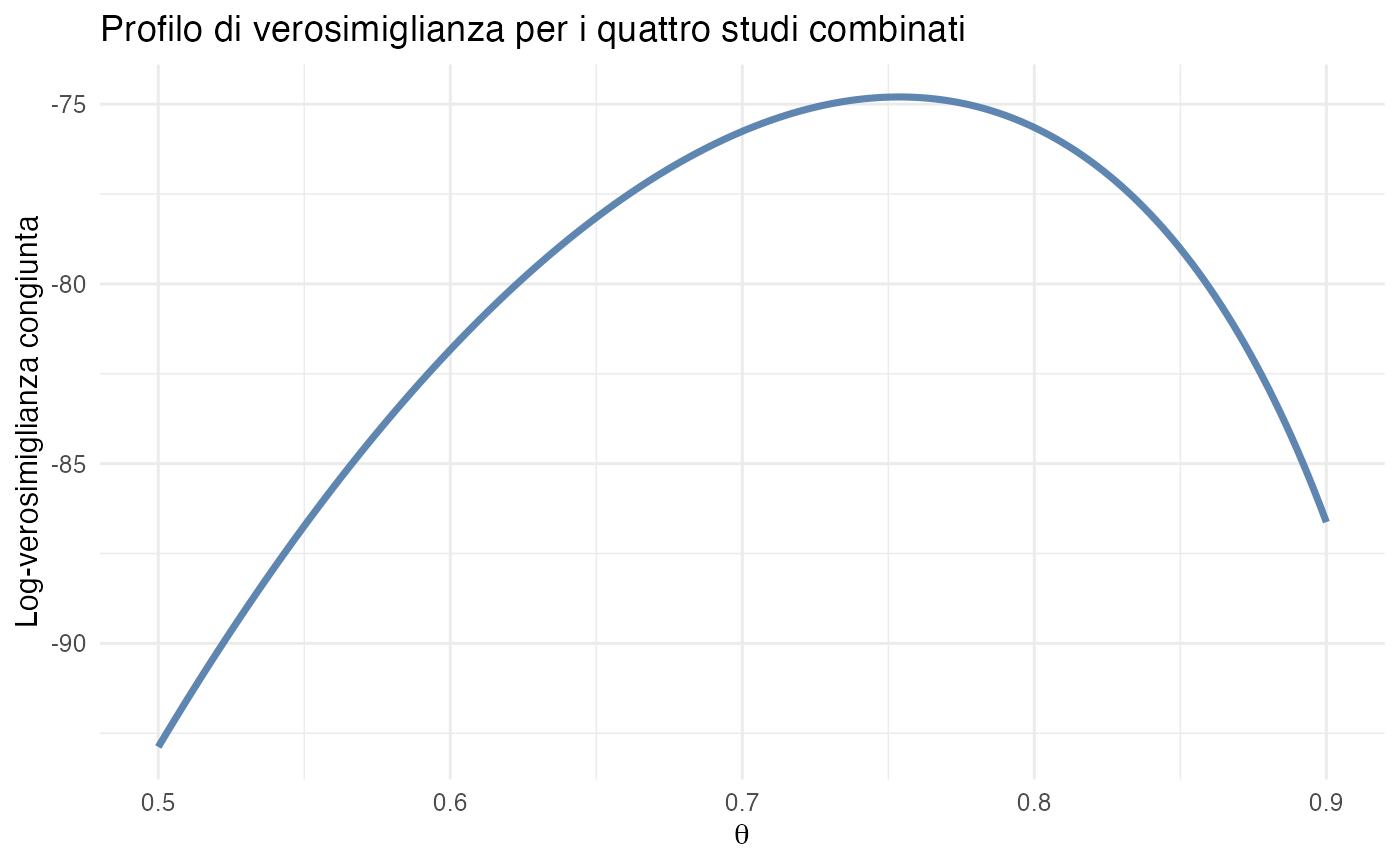
\includegraphics[width=0.85\linewidth,height=\textheight,keepaspectratio]{chapters/probability/14_likelihood_files/figure-pdf/unnamed-chunk-6-1.png}
\end{center}

\begin{Shaded}
\begin{Highlighting}[]
\CommentTok{\# Calcolo della MLE combinata tramite ottimizzazione numerica}
\NormalTok{result }\OtherTok{\textless{}{-}} \FunctionTok{optim}\NormalTok{(}
  \AttributeTok{par =} \FloatTok{0.7}\NormalTok{,}
  \AttributeTok{fn =} \ControlFlowTok{function}\NormalTok{(t) }\SpecialCharTok{{-}}\FunctionTok{log\_lik\_congiunta}\NormalTok{(t),  }\CommentTok{\# Minimizziamo la negativa}
  \AttributeTok{method =} \StringTok{"Brent"}\NormalTok{,}
  \AttributeTok{lower =} \FloatTok{0.5}\NormalTok{,}
  \AttributeTok{upper =} \FloatTok{0.9}
\NormalTok{)}

\FunctionTok{cat}\NormalTok{(}\StringTok{"Stima di massima verosimiglianza (combinata):"}\NormalTok{, }\FunctionTok{round}\NormalTok{(result}\SpecialCharTok{$}\NormalTok{par, }\DecValTok{4}\NormalTok{), }\StringTok{"}\SpecialCharTok{\textbackslash{}n}\StringTok{"}\NormalTok{)}
\CommentTok{\#\textgreater{} Stima di massima verosimiglianza (combinata): 0.754}
\FunctionTok{cat}\NormalTok{(}\StringTok{"Proporzione complessiva (successi/prove):"}\NormalTok{, }
    \FunctionTok{round}\NormalTok{(}\FunctionTok{sum}\NormalTok{(studi}\SpecialCharTok{$}\NormalTok{successi) }\SpecialCharTok{/} \FunctionTok{sum}\NormalTok{(studi}\SpecialCharTok{$}\NormalTok{prove), }\DecValTok{4}\NormalTok{), }\StringTok{"}\SpecialCharTok{\textbackslash{}n}\StringTok{"}\NormalTok{)}
\CommentTok{\#\textgreater{} Proporzione complessiva (successi/prove): 0.754}
\end{Highlighting}
\end{Shaded}

La stima risultante rappresenta il valore di \(\theta\) più plausibile
alla luce di \textbf{tutti i dati considerati insieme}, illustrando così
come la verosimiglianza fornisca un meccanismo naturale per
l'integrazione di evidenze multiple.

\section{Verosimiglianza gaussiana}\label{verosimiglianza-gaussiana}

La distribuzione gaussiana è uno strumento fondamentale della
statistica. La sua importanza deriva dalla capacità di descrivere in
modo efficace molte variabili continue di interesse psicologico e
scientifico, come il quoziente intellettivo (QI), i tempi di reazione e
diverse misurazioni psicofisiologiche.

\subsection{Caso di una singola
osservazione}\label{caso-di-una-singola-osservazione}

Consideriamo una variabile normale con media incognita \(\mu\) e
deviazione standard nota \(\sigma\). Per una singola osservazione \(y\),
la verosimiglianza è: \[
L(\mu \mid y) = \frac{1}{\sigma\sqrt{2\pi}} \exp\left(-\frac{(y-\mu)^2}{2\sigma^2}\right).
\]

Vista come funzione di \(\mu\), questa è una curva a campana centrata
sul valore osservato \(y\).

\begin{Shaded}
\begin{Highlighting}[]
\NormalTok{y\_obs }\OtherTok{\textless{}{-}} \DecValTok{114}
\NormalTok{sigma }\OtherTok{\textless{}{-}} \DecValTok{15}
\NormalTok{mu\_grid }\OtherTok{\textless{}{-}} \FunctionTok{seq}\NormalTok{(}\DecValTok{70}\NormalTok{, }\DecValTok{160}\NormalTok{, }\AttributeTok{length.out =} \DecValTok{500}\NormalTok{)}
\NormalTok{likelihood }\OtherTok{\textless{}{-}} \FunctionTok{dnorm}\NormalTok{(y\_obs, }\AttributeTok{mean =}\NormalTok{ mu\_grid, }\AttributeTok{sd =}\NormalTok{ sigma)}

\FunctionTok{ggplot}\NormalTok{(}\FunctionTok{data.frame}\NormalTok{(}\AttributeTok{mu =}\NormalTok{ mu\_grid, }\AttributeTok{lik =}\NormalTok{ likelihood), }\FunctionTok{aes}\NormalTok{(}\AttributeTok{x =}\NormalTok{ mu, }\AttributeTok{y =}\NormalTok{ lik)) }\SpecialCharTok{+}
  \FunctionTok{geom\_line}\NormalTok{(}\AttributeTok{linewidth =} \FloatTok{1.2}\NormalTok{, }\AttributeTok{color =} \StringTok{"\#4E79A7"}\NormalTok{) }\SpecialCharTok{+}
  \FunctionTok{geom\_vline}\NormalTok{(}\AttributeTok{xintercept =}\NormalTok{ y\_obs, }\AttributeTok{linetype =} \StringTok{"dashed"}\NormalTok{, }\AttributeTok{color =} \StringTok{"\#E15759"}\NormalTok{) }\SpecialCharTok{+}
  \FunctionTok{labs}\NormalTok{(}
    \AttributeTok{x =} \FunctionTok{expression}\NormalTok{(mu),}
    \AttributeTok{y =} \StringTok{"Verosimiglianza"}
\NormalTok{  ) }\SpecialCharTok{+}
  \FunctionTok{theme\_minimal}\NormalTok{()}
\end{Highlighting}
\end{Shaded}

\begin{figure}[H]

\centering{

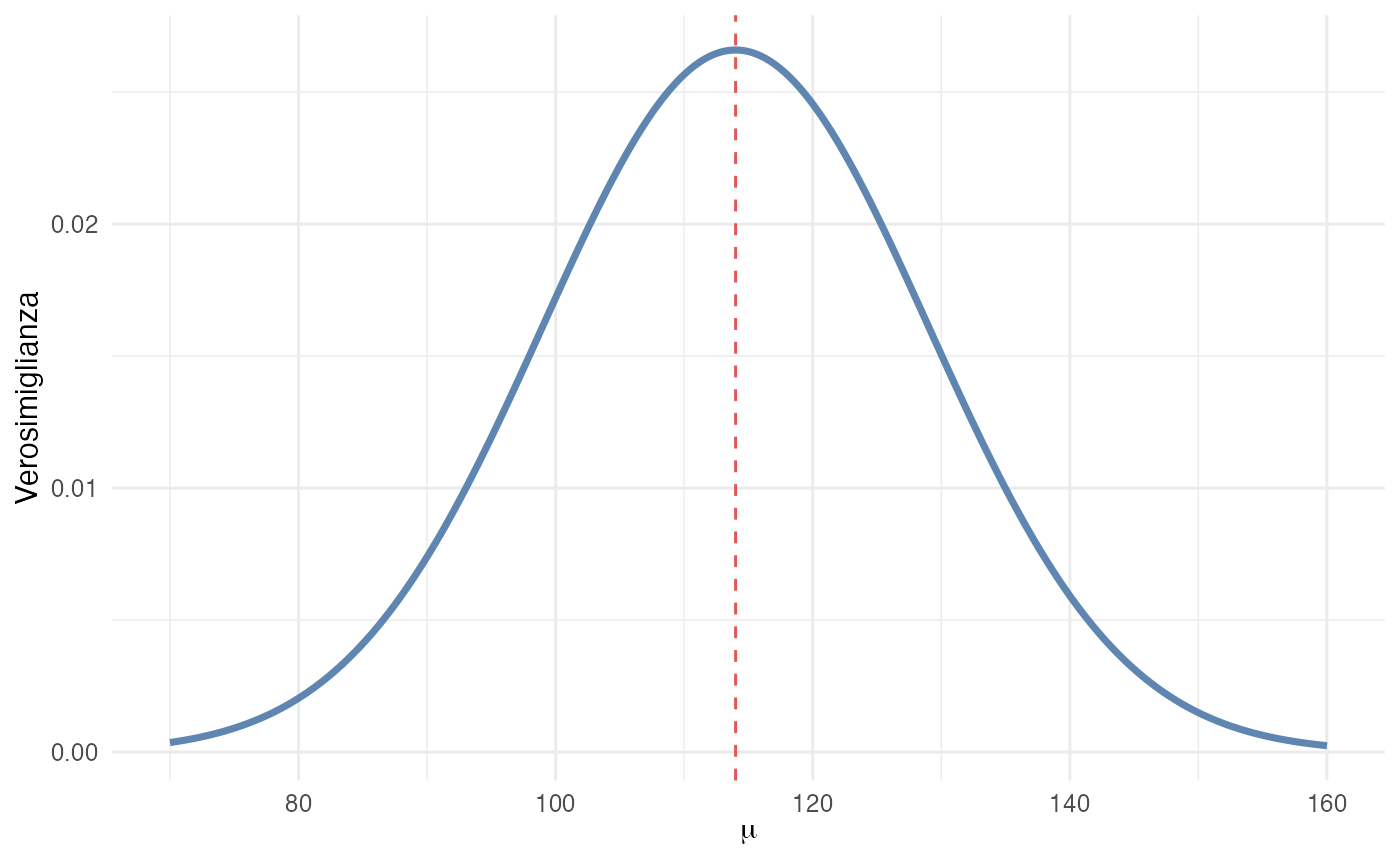
\includegraphics[width=0.85\linewidth,height=\textheight,keepaspectratio]{chapters/probability/14_likelihood_files/figure-pdf/fig-normal-lik-single-1.png}

}

\caption{\label{fig-normal-lik-single}Verosimiglianza gaussiana per una
singola osservazione. Il massimo si trova esattamente nel punto
osservato.}

\end{figure}%

\subsection{Caso di un campione
gaussiano}\label{caso-di-un-campione-gaussiano}

Per un campione di \(n\) osservazioni indipendenti e identicamente
distribuite (i.i.d.) \(y_1, \ldots, y_n\) provenienti da una
distribuzione Normale \(\mathcal{N}(\mu, \sigma^2)\) con varianza
\(\sigma^2\) nota, la \textbf{funzione di verosimiglianza} è il prodotto
delle densità individuali:

\[
L(\mu; y_1, \ldots, y_n) = \prod_{i=1}^n \frac{1}{\sqrt{2\pi\sigma^2}} \exp\left[-\frac{1}{2\sigma^2}(y_i - \mu)^2\right].
\]

Per semplificare i calcoli analitici, si considera la
\textbf{log-verosimiglianza}, che trasforma il prodotto in una somma:

\[
\ell(\mu) = \log L(\mu; y_1, \ldots, y_n) = -\frac{n}{2}\log(2\pi\sigma^2) - \frac{1}{2\sigma^2}\sum_{i=1}^n (y_i - \mu)^2.
\]

Per ottenere lo stimatore di massima verosimiglianza (MLE) è necessario
massimizzare \(\ell(\mu)\) rispetto a \(\mu\). Ciò equivale a
\textbf{minimizzare} la somma dei quadrati degli scarti
\(\sum_{i=1}^n (y_i - \mu)^2\). Derivando e ponendo uguale a zero, si
ottiene:

\[
\hat{\mu}_{\text{MLE}} = \frac{1}{n} \sum_{i=1}^n y_i = \bar{y}.
\]

Pertanto, nel caso di una distribuzione gaussiana con varianza nota, lo
stimatore di massima verosimiglianza per la media \(\mu\) coincide con
la media campionaria.

Questo risultato può essere facilmente verificato mediante una
simulazione numerica in R.

\begin{Shaded}
\begin{Highlighting}[]
\CommentTok{\# Dati simulati (punteggi BDI{-}II)}
\FunctionTok{set.seed}\NormalTok{(}\DecValTok{42}\NormalTok{)}
\NormalTok{y }\OtherTok{\textless{}{-}} \FunctionTok{c}\NormalTok{(}\DecValTok{26}\NormalTok{, }\DecValTok{35}\NormalTok{, }\DecValTok{30}\NormalTok{, }\DecValTok{25}\NormalTok{, }\DecValTok{44}\NormalTok{, }\DecValTok{30}\NormalTok{, }\DecValTok{33}\NormalTok{, }\DecValTok{43}\NormalTok{, }\DecValTok{22}\NormalTok{, }\DecValTok{43}\NormalTok{, }\DecValTok{24}\NormalTok{, }\DecValTok{19}\NormalTok{, }\DecValTok{39}\NormalTok{, }\DecValTok{31}\NormalTok{, }\DecValTok{25}\NormalTok{,}
       \DecValTok{28}\NormalTok{, }\DecValTok{35}\NormalTok{, }\DecValTok{30}\NormalTok{, }\DecValTok{26}\NormalTok{, }\DecValTok{31}\NormalTok{, }\DecValTok{41}\NormalTok{, }\DecValTok{36}\NormalTok{, }\DecValTok{26}\NormalTok{, }\DecValTok{35}\NormalTok{, }\DecValTok{33}\NormalTok{, }\DecValTok{28}\NormalTok{, }\DecValTok{27}\NormalTok{, }\DecValTok{34}\NormalTok{, }\DecValTok{27}\NormalTok{, }\DecValTok{22}\NormalTok{)}
\NormalTok{sigma }\OtherTok{\textless{}{-}} \FloatTok{6.5}

\CommentTok{\# Log{-}verosimiglianza}
\NormalTok{log\_lik }\OtherTok{\textless{}{-}} \ControlFlowTok{function}\NormalTok{(mu) \{}
  \FunctionTok{sum}\NormalTok{(}\FunctionTok{dnorm}\NormalTok{(y, }\AttributeTok{mean =}\NormalTok{ mu, }\AttributeTok{sd =}\NormalTok{ sigma, }\AttributeTok{log =} \ConstantTok{TRUE}\NormalTok{))}
\NormalTok{\}}

\NormalTok{mu\_grid }\OtherTok{\textless{}{-}} \FunctionTok{seq}\NormalTok{(}\DecValTok{25}\NormalTok{, }\DecValTok{40}\NormalTok{, }\AttributeTok{length.out =} \DecValTok{200}\NormalTok{)}
\NormalTok{ll\_vals }\OtherTok{\textless{}{-}} \FunctionTok{sapply}\NormalTok{(mu\_grid, log\_lik)}

\FunctionTok{ggplot}\NormalTok{(}\FunctionTok{data.frame}\NormalTok{(}\AttributeTok{mu =}\NormalTok{ mu\_grid, }\AttributeTok{ll =}\NormalTok{ ll\_vals), }\FunctionTok{aes}\NormalTok{(}\AttributeTok{x =}\NormalTok{ mu, }\AttributeTok{y =}\NormalTok{ ll)) }\SpecialCharTok{+}
  \FunctionTok{geom\_line}\NormalTok{(}\AttributeTok{linewidth =} \FloatTok{1.2}\NormalTok{, }\AttributeTok{color =} \StringTok{"\#4E79A7"}\NormalTok{) }\SpecialCharTok{+}
  \FunctionTok{geom\_vline}\NormalTok{(}\AttributeTok{xintercept =} \FunctionTok{mean}\NormalTok{(y), }\AttributeTok{linetype =} \StringTok{"dashed"}\NormalTok{, }\AttributeTok{color =} \StringTok{"\#E15759"}\NormalTok{) }\SpecialCharTok{+}
  \FunctionTok{annotate}\NormalTok{(}\StringTok{"text"}\NormalTok{, }\AttributeTok{x =} \FunctionTok{mean}\NormalTok{(y) }\SpecialCharTok{+} \FloatTok{0.3}\NormalTok{, }\AttributeTok{y =} \FunctionTok{max}\NormalTok{(ll\_vals) }\SpecialCharTok{{-}} \DecValTok{10}\NormalTok{,}
           \AttributeTok{label =} \FunctionTok{paste0}\NormalTok{(}\StringTok{"Media = "}\NormalTok{, }\FunctionTok{round}\NormalTok{(}\FunctionTok{mean}\NormalTok{(y), }\DecValTok{2}\NormalTok{)), }
           \AttributeTok{color =} \StringTok{"\#E15759"}\NormalTok{, }\AttributeTok{hjust =} \DecValTok{0}\NormalTok{) }\SpecialCharTok{+}
  \FunctionTok{labs}\NormalTok{(}
    \AttributeTok{x =} \FunctionTok{expression}\NormalTok{(mu),}
    \AttributeTok{y =} \StringTok{"Log{-}verosimiglianza"}
\NormalTok{  ) }\SpecialCharTok{+}
  \FunctionTok{theme\_minimal}\NormalTok{()}
\end{Highlighting}
\end{Shaded}

\begin{figure}[H]

\centering{

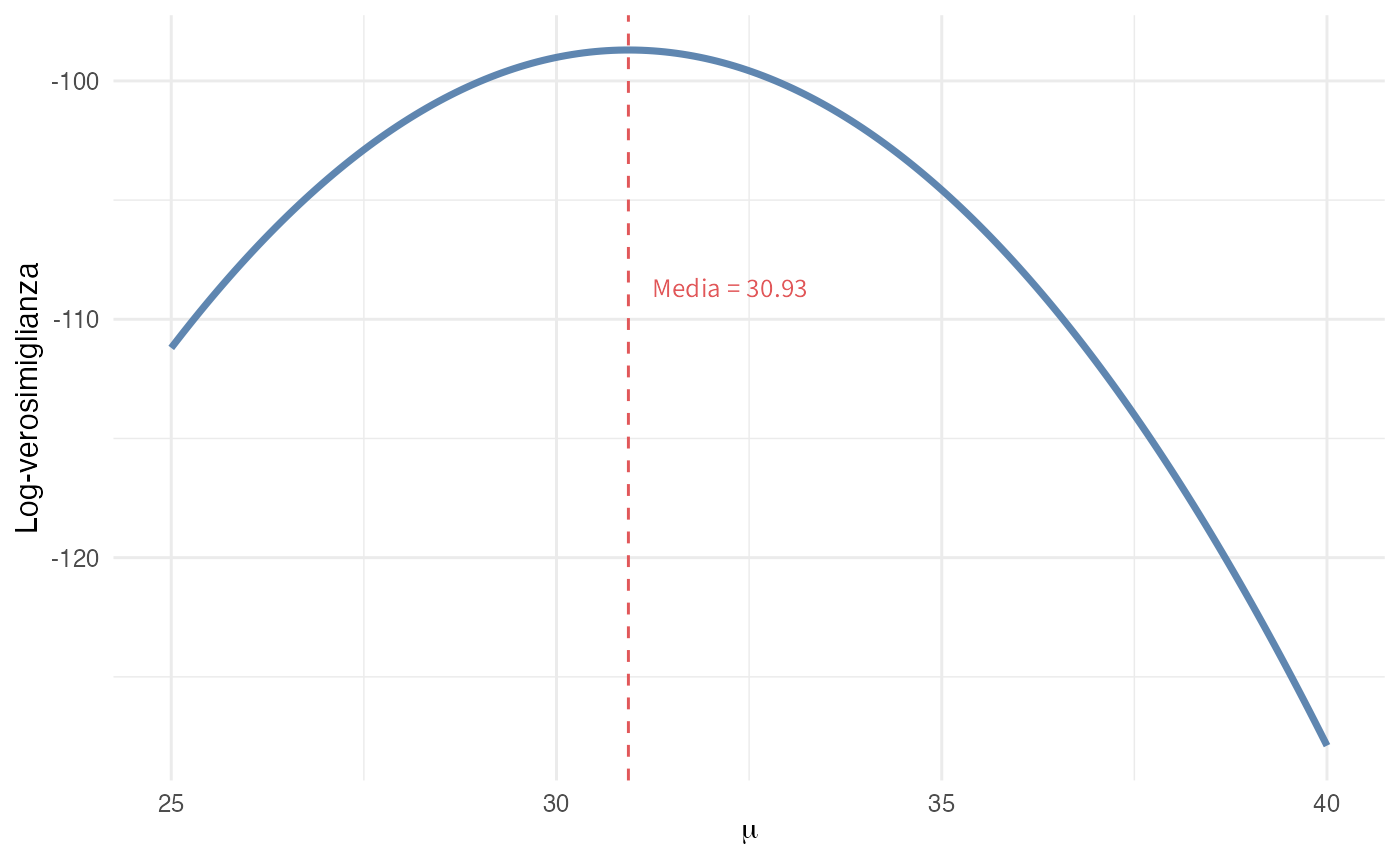
\includegraphics[width=0.85\linewidth,height=\textheight,keepaspectratio]{chapters/probability/14_likelihood_files/figure-pdf/fig-normal-lik-sample-1.png}

}

\caption{\label{fig-normal-lik-sample}Log-verosimiglianza per un
campione di 30 osservazioni. Il massimo corrisponde alla media
campionaria.}

\end{figure}%

\begin{tcolorbox}[enhanced jigsaw, arc=.35mm, breakable, colbacktitle=quarto-callout-note-color!10!white, opacityback=0, toprule=.15mm, rightrule=.15mm, colback=white, opacitybacktitle=0.6, leftrule=.75mm, coltitle=black, bottomtitle=1mm, left=2mm, toptitle=1mm, title=\textcolor{quarto-callout-note-color}{\faInfo}\hspace{0.5em}{La forma della verosimiglianza gaussiana}, titlerule=0mm, bottomrule=.15mm, colframe=quarto-callout-note-color-frame]

Nel caso gaussiano, la log-verosimiglianza è una \textbf{parabola} in
\(\mu\): una funzione quadratica con concavità verso il basso, il cui
vertice corrisponde alla media campionaria. Poiché la verosimiglianza è
l'esponenziale della log-verosimiglianza, essa assume la forma di una
\textbf{curva a campana gaussiana} centrata su \(\bar{y}\).

L'\textbf{ampiezza} di questa campana, ovvero quanto è larga o stretta,
dipende da due fattori: la variabilità intrinseca delle osservazioni
(\(\sigma^2\)) e il numero di dati raccolti (\(n\)). In termini precisi,
la verosimiglianza, vista come funzione di \(\mu\), è una gaussiana con
varianza \(\sigma^2/n\).

Questa proprietà è cruciale: nel prossimo capitolo vedremo come la
quantità \(\sigma^2/n\) determina direttamente la precisione della
distribuzione a posteriori, stabilendo il collegamento formale tra
verosimiglianza e l'aggiornamento bayesiano.

\end{tcolorbox}

\section{Il rapporto di
verosimiglianze}\label{il-rapporto-di-verosimiglianze}

In statistica è frequente voler confrontare due ipotesi specifiche sui
parametri di un modello scelto per descrivere i dati osservati. Una
delle strategie più dirette per farlo consiste nel valutare
\textbf{quanto bene ciascuna ipotesi spiega i dati}: questo è
esattamente ciò che misura il \emph{rapporto di verosimiglianze}.

\subsection{Confronto tra due ipotesi
puntuali}\label{confronto-tra-due-ipotesi-puntuali}

Dato un modello e due ipotesi alternative sui parametri, \(\theta_0\) e
\(\theta_1\), il \textbf{rapporto di verosimiglianze} è definito come:

\[
\Lambda = \frac{L(\theta_1 \mid \text{dati})}{L(\theta_0 \mid \text{dati})}.
\]

Si tratta, quindi, di un confronto diretto tra le verosimiglianze: il
numeratore indica quanto i dati sono plausibili assumendo \(\theta_1\),
mentre il denominatore indica quanto lo sono assumendo \(\theta_0\).

\subsection{Interpretazione}\label{interpretazione}

\begin{itemize}
\tightlist
\item
  \textbf{\(\Lambda > 1\)}: i dati sono più probabili sotto \(\theta_1\)
  rispetto a \(\theta_0\); quindi l'evidenza relativa favorisce
  \(\theta_1\);
\item
  \textbf{\(\Lambda < 1\)}: i dati sono più probabili sotto
  \(\theta_0\); quindi l'evidenza relativa favorisce \(\theta_0\);
\item
  \textbf{\(\Lambda \approx 1\)}: le due ipotesi hanno un potere
  esplicativo simile; quindi i dati non permettono di discriminare in
  modo netto tra loro.
\end{itemize}

La distanza dall'unità indica quanto un'ipotesi renda i dati più (o
meno) plausibili rispetto all'altra. In questo modo, il rapporto di
verosimiglianze fornisce una misura continua e graduata della forza
dell'evidenza empirica, evitando valutazioni dicotomiche e mettendo in
primo piano il contributo informativo dei dati.

\subsection{Esempio: moneta equilibrata
vs.~sbilanciata}\label{esempio-moneta-equilibrata-vs.-sbilanciata}

Supponiamo di osservare \(x = 7\) successi su \(n = 10\) lanci.
Confrontiamo due modelli:

\begin{itemize}
\tightlist
\item
  \(H_0\): moneta equilibrata (\(\theta_0 = 0.5\));
\item
  \(H_1\): moneta sbilanciata (\(\theta_1 = 0.7\)).
\end{itemize}

\begin{Shaded}
\begin{Highlighting}[]
\NormalTok{n }\OtherTok{\textless{}{-}} \DecValTok{10}
\NormalTok{y }\OtherTok{\textless{}{-}} \DecValTok{7}

\NormalTok{L\_H0 }\OtherTok{\textless{}{-}} \FunctionTok{dbinom}\NormalTok{(y, n, }\AttributeTok{prob =} \FloatTok{0.5}\NormalTok{)}
\NormalTok{L\_H1 }\OtherTok{\textless{}{-}} \FunctionTok{dbinom}\NormalTok{(y, n, }\AttributeTok{prob =} \FloatTok{0.7}\NormalTok{)}
\NormalTok{LR }\OtherTok{\textless{}{-}}\NormalTok{ L\_H1 }\SpecialCharTok{/}\NormalTok{ L\_H0}

\FunctionTok{cat}\NormalTok{(}\StringTok{"L(H0):"}\NormalTok{, }\FunctionTok{round}\NormalTok{(L\_H0, }\DecValTok{4}\NormalTok{), }\StringTok{"}\SpecialCharTok{\textbackslash{}n}\StringTok{"}\NormalTok{)}
\CommentTok{\#\textgreater{} L(H0): 0.117}
\FunctionTok{cat}\NormalTok{(}\StringTok{"L(H1):"}\NormalTok{, }\FunctionTok{round}\NormalTok{(L\_H1, }\DecValTok{4}\NormalTok{), }\StringTok{"}\SpecialCharTok{\textbackslash{}n}\StringTok{"}\NormalTok{)}
\CommentTok{\#\textgreater{} L(H1): 0.267}
\FunctionTok{cat}\NormalTok{(}\StringTok{"Rapporto di verosimiglianze:"}\NormalTok{, }\FunctionTok{round}\NormalTok{(LR, }\DecValTok{2}\NormalTok{), }\StringTok{"}\SpecialCharTok{\textbackslash{}n}\StringTok{"}\NormalTok{)}
\CommentTok{\#\textgreater{} Rapporto di verosimiglianze: 2.28}
\end{Highlighting}
\end{Shaded}

Il rapporto di circa 2.3 indica che i dati sono circa 2.3 volte più
probabili sotto \(H_1\) rispetto a \(H_0\). È un'evidenza moderata a
favore della moneta sbilanciata.

\begin{Shaded}
\begin{Highlighting}[]
\NormalTok{theta\_seq }\OtherTok{\textless{}{-}} \FunctionTok{seq}\NormalTok{(}\DecValTok{0}\NormalTok{, }\DecValTok{1}\NormalTok{, }\AttributeTok{length.out =} \DecValTok{500}\NormalTok{)}
\NormalTok{lik\_vals }\OtherTok{\textless{}{-}} \FunctionTok{dbinom}\NormalTok{(y, n, }\AttributeTok{prob =}\NormalTok{ theta\_seq)}

\FunctionTok{ggplot}\NormalTok{(}\FunctionTok{data.frame}\NormalTok{(}\AttributeTok{theta =}\NormalTok{ theta\_seq, }\AttributeTok{lik =}\NormalTok{ lik\_vals), }\FunctionTok{aes}\NormalTok{(}\AttributeTok{x =}\NormalTok{ theta, }\AttributeTok{y =}\NormalTok{ lik)) }\SpecialCharTok{+}
  \FunctionTok{geom\_line}\NormalTok{(}\AttributeTok{linewidth =} \FloatTok{1.2}\NormalTok{, }\AttributeTok{color =} \StringTok{"\#4E79A7"}\NormalTok{) }\SpecialCharTok{+}
  \FunctionTok{geom\_point}\NormalTok{(}\FunctionTok{aes}\NormalTok{(}\AttributeTok{x =} \FloatTok{0.5}\NormalTok{, }\AttributeTok{y =}\NormalTok{ L\_H0), }\AttributeTok{color =} \StringTok{"\#E15759"}\NormalTok{, }\AttributeTok{size =} \DecValTok{3}\NormalTok{) }\SpecialCharTok{+}
  \FunctionTok{geom\_point}\NormalTok{(}\FunctionTok{aes}\NormalTok{(}\AttributeTok{x =} \FloatTok{0.7}\NormalTok{, }\AttributeTok{y =}\NormalTok{ L\_H1), }\AttributeTok{color =} \StringTok{"\#59A14F"}\NormalTok{, }\AttributeTok{size =} \DecValTok{3}\NormalTok{) }\SpecialCharTok{+}
  \FunctionTok{geom\_segment}\NormalTok{(}\FunctionTok{aes}\NormalTok{(}\AttributeTok{x =} \FloatTok{0.5}\NormalTok{, }\AttributeTok{xend =} \FloatTok{0.5}\NormalTok{, }\AttributeTok{y =} \DecValTok{0}\NormalTok{, }\AttributeTok{yend =}\NormalTok{ L\_H0),}
               \AttributeTok{linetype =} \StringTok{"dashed"}\NormalTok{, }\AttributeTok{color =} \StringTok{"\#E15759"}\NormalTok{) }\SpecialCharTok{+}
  \FunctionTok{geom\_segment}\NormalTok{(}\FunctionTok{aes}\NormalTok{(}\AttributeTok{x =} \FloatTok{0.7}\NormalTok{, }\AttributeTok{xend =} \FloatTok{0.7}\NormalTok{, }\AttributeTok{y =} \DecValTok{0}\NormalTok{, }\AttributeTok{yend =}\NormalTok{ L\_H1),}
               \AttributeTok{linetype =} \StringTok{"dashed"}\NormalTok{, }\AttributeTok{color =} \StringTok{"\#59A14F"}\NormalTok{) }\SpecialCharTok{+}
  \FunctionTok{annotate}\NormalTok{(}\StringTok{"text"}\NormalTok{, }\AttributeTok{x =} \FloatTok{0.5}\NormalTok{, }\AttributeTok{y =}\NormalTok{ L\_H0 }\SpecialCharTok{+} \FloatTok{0.02}\NormalTok{, }\AttributeTok{label =} \StringTok{"H0"}\NormalTok{, }\AttributeTok{color =} \StringTok{"\#E15759"}\NormalTok{) }\SpecialCharTok{+}
  \FunctionTok{annotate}\NormalTok{(}\StringTok{"text"}\NormalTok{, }\AttributeTok{x =} \FloatTok{0.7}\NormalTok{, }\AttributeTok{y =}\NormalTok{ L\_H1 }\SpecialCharTok{+} \FloatTok{0.02}\NormalTok{, }\AttributeTok{label =} \StringTok{"H1"}\NormalTok{, }\AttributeTok{color =} \StringTok{"\#59A14F"}\NormalTok{) }\SpecialCharTok{+}
  \FunctionTok{labs}\NormalTok{(}
    \AttributeTok{x =} \FunctionTok{expression}\NormalTok{(theta),}
    \AttributeTok{y =} \StringTok{"Verosimiglianza"}
\NormalTok{  ) }\SpecialCharTok{+}
  \FunctionTok{theme\_minimal}\NormalTok{()}
\end{Highlighting}
\end{Shaded}

\begin{figure}[H]

\centering{

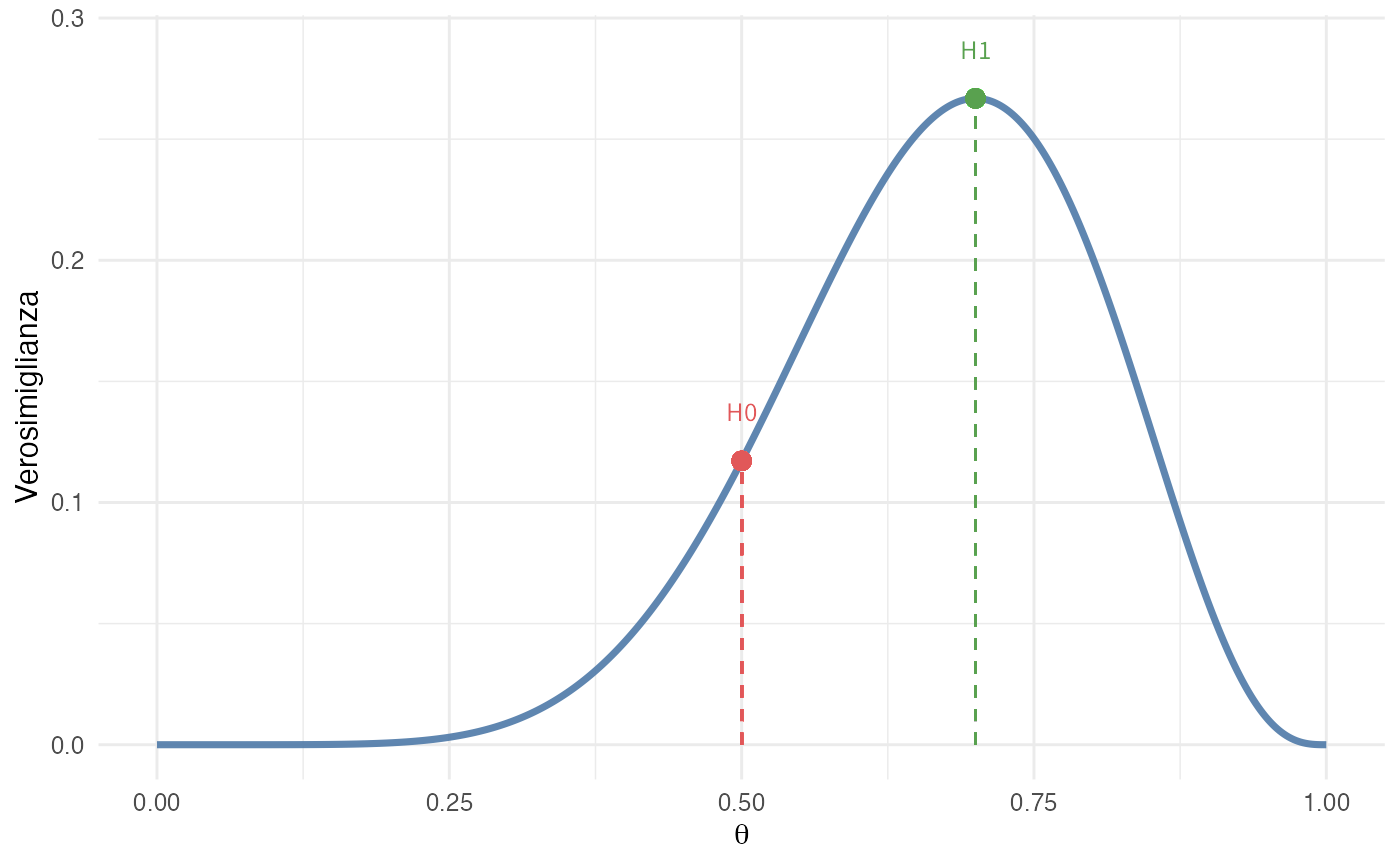
\includegraphics[width=0.85\linewidth,height=\textheight,keepaspectratio]{chapters/probability/14_likelihood_files/figure-pdf/fig-lr-1.png}

}

\caption{\label{fig-lr}Funzione di verosimiglianza con i due valori
parametrici confrontati. Il rapporto delle altezze nei due punti è il
rapporto di verosimiglianze.}

\end{figure}%

\subsection{Connessione con l'inferenza
bayesiana}\label{connessione-con-linferenza-bayesiana}

Con distribuzioni a priori uniformi (non informative), il rapporto di
verosimiglianze coincide con il \textbf{fattore di Bayes}, uno strumento
utilizzato in ambito bayesiano per il confronto di modelli : \[
BF_{10} = \frac{P(\text{dati} \mid H_1)}{P(\text{dati} \mid H_0)}.
\]

\section{Il criterio di informazione di Akaike
(AIC)}\label{il-criterio-di-informazione-di-akaike-aic}

Il \emph{Criterio di Informazione di Akaike (AIC)} fornisce una
soluzione semplice per il problema della selezione dei modelli.

\subsection{Il problema
dell'overfitting}\label{il-problema-delloverfitting}

Quando si confrontano modelli, quelli più complessi (con un maggior
numero di parametri) tendono ad adattarsi meglio ai dati. Tuttavia,
questo vantaggio può riflettere solo una maggiore flessibilità e non una
reale capacità esplicativa. Questo fenomeno è noto come
``sovradattamento'' (\emph{overfitting}) e richiede quindi criteri che
penalizzino opportunamente la complessità.

\subsection{Definizione dell'AIC}\label{definizione-dellaic}

Il \textbf{Criterio di Informazione di Akaike (AIC)} fornisce una misura
per confrontare modelli statistici, conciliando la bontà di adattamento
ai dati con la loro complessità:

\[
\text{AIC} = 2k - 2\log(\hat{L}),
\] dove \(k\) è il numero di parametri stimati del modello e \(\hat{L}\)
rappresenta il valore massimo della funzione di verosimiglianza per quel
modello.

La formula unisce due principi fondamentali dell'inferenza statistica.
Il termine \(-2\log(\hat{L})\) misura la mancanza di adattamento (lack
of fit): valori minori indicano una maggiore compatibilità del modello
con i dati. Il termine \(2k\) opera invece come una penalità per la
complessità, penalizzando i modelli con un numero elevato di parametri e
promuovendo la parsimonia. In sostanza, l'AIC rappresenta un compromesso
tra capacità esplicativa e semplicità, premiando i modelli che
descrivono bene i dati utilizzando un numero minore di parametri.

\textbf{Interpretazione:} nel confronto tra modelli, viene preferito il
modello con il valore AIC \textbf{più basso}. La penalità \(2k\)
garantisce che un adattamento ai dati leggermente migliore, ma ottenuto
aggiungendo molti parametri, non venga considerato un reale
miglioramento del modello, promuovendo il principio di parsimonia.

\subsection{Esempio: effetto del contenuto emotivo sulla
memoria}\label{esempio-effetto-del-contenuto-emotivo-sulla-memoria}

Supponiamo di voler valutare l'effetto del contenuto emotivo delle
immagini sulla memoria visiva. In un esperimento controllato, 30
partecipanti per condizione hanno mostrato i seguenti risultati:

\begin{Shaded}
\begin{Highlighting}[]
\CommentTok{\# Dati sperimentali}
\NormalTok{successi\_neutro }\OtherTok{\textless{}{-}} \DecValTok{14}
\NormalTok{successi\_emozione }\OtherTok{\textless{}{-}} \DecValTok{22}
\NormalTok{n }\OtherTok{\textless{}{-}} \DecValTok{30}
\end{Highlighting}
\end{Shaded}

Il modello nullo ipotizza che il contenuto emotivo non influenzi la
memoria, postulando una probabilità comune per entrambe le condizioni:

\begin{Shaded}
\begin{Highlighting}[]
\CommentTok{\# Modello nullo: stessa probabilità per entrambi}
\NormalTok{p\_null }\OtherTok{\textless{}{-}}\NormalTok{ (successi\_neutro }\SpecialCharTok{+}\NormalTok{ successi\_emozione) }\SpecialCharTok{/}\NormalTok{ (}\DecValTok{2} \SpecialCharTok{*}\NormalTok{ n)}
\NormalTok{ll\_null }\OtherTok{\textless{}{-}} \FunctionTok{dbinom}\NormalTok{(successi\_neutro, n, p\_null, }\AttributeTok{log =} \ConstantTok{TRUE}\NormalTok{) }\SpecialCharTok{+}
           \FunctionTok{dbinom}\NormalTok{(successi\_emozione, n, p\_null, }\AttributeTok{log =} \ConstantTok{TRUE}\NormalTok{)}
\NormalTok{AIC\_null }\OtherTok{\textless{}{-}} \DecValTok{2} \SpecialCharTok{*} \DecValTok{1} \SpecialCharTok{{-}} \DecValTok{2} \SpecialCharTok{*}\NormalTok{ ll\_null  }\CommentTok{\# 1 parametro}
\end{Highlighting}
\end{Shaded}

Il modello alternativo consente probabilità differenziate, riconoscendo
il possibile effetto dell'emozione:

\begin{Shaded}
\begin{Highlighting}[]
\CommentTok{\# Modello alternativo: probabilità diverse}
\NormalTok{p1 }\OtherTok{\textless{}{-}}\NormalTok{ successi\_neutro }\SpecialCharTok{/}\NormalTok{ n}
\NormalTok{p2 }\OtherTok{\textless{}{-}}\NormalTok{ successi\_emozione }\SpecialCharTok{/}\NormalTok{ n}
\NormalTok{ll\_alt }\OtherTok{\textless{}{-}} \FunctionTok{dbinom}\NormalTok{(successi\_neutro, n, p1, }\AttributeTok{log =} \ConstantTok{TRUE}\NormalTok{) }\SpecialCharTok{+}
          \FunctionTok{dbinom}\NormalTok{(successi\_emozione, n, p2, }\AttributeTok{log =} \ConstantTok{TRUE}\NormalTok{)}
\NormalTok{AIC\_alt }\OtherTok{\textless{}{-}} \DecValTok{2} \SpecialCharTok{*} \DecValTok{2} \SpecialCharTok{{-}} \DecValTok{2} \SpecialCharTok{*}\NormalTok{ ll\_alt  }\CommentTok{\# 2 parametri}
\end{Highlighting}
\end{Shaded}

La valutazione mediante AIC bilancia adattamento e complessità:

\begin{Shaded}
\begin{Highlighting}[]
\FunctionTok{cat}\NormalTok{(}\StringTok{"Modello nullo {-} AIC:"}\NormalTok{, }\FunctionTok{round}\NormalTok{(AIC\_null, }\DecValTok{2}\NormalTok{), }\StringTok{"}\SpecialCharTok{\textbackslash{}n}\StringTok{"}\NormalTok{)}
\CommentTok{\#\textgreater{} Modello nullo {-} AIC: 14}
\FunctionTok{cat}\NormalTok{(}\StringTok{"Modello alternativo {-} AIC:"}\NormalTok{, }\FunctionTok{round}\NormalTok{(AIC\_alt, }\DecValTok{2}\NormalTok{), }\StringTok{"}\SpecialCharTok{\textbackslash{}n}\StringTok{"}\NormalTok{)}
\CommentTok{\#\textgreater{} Modello alternativo {-} AIC: 11.5}
\FunctionTok{cat}\NormalTok{(}\StringTok{"Differenza (ΔAIC):"}\NormalTok{, }\FunctionTok{round}\NormalTok{(AIC\_alt }\SpecialCharTok{{-}}\NormalTok{ AIC\_null, }\DecValTok{2}\NormalTok{), }\StringTok{"}\SpecialCharTok{\textbackslash{}n}\StringTok{"}\NormalTok{)}
\CommentTok{\#\textgreater{} Differenza (ΔAIC): {-}2.51}
\end{Highlighting}
\end{Shaded}

Una differenza AIC negativa indica che il modello alternativo è
preferibile nonostante abbia un parametro in più. L'evidenza suggerisce
che il modello che assegna probabilità distinte ai due gruppi descrive
meglio i dati osservati.

\section*{Riflessioni conclusive}\label{riflessioni-conclusive-12}

\markright{Riflessioni conclusive}

La funzione di verosimiglianza è il concetto centrale che collega i dati
ai parametri nell'inferenza statistica. Per ogni possibile valore del
parametro, essa quantifica quanto i dati osservati siano compatibili con
quel valore, offrendo una mappa di plausibilità basata sull'evidenza
empirica.

In questo capitolo abbiamo esplorato le caratteristiche di base della
verosimiglianza. Abbiamo visto che la funzione di verosimiglianza
\textbf{inverte} la prospettiva della funzione di probabilità: non ci
chiediamo quali dati possiamo aspettarci in base al parametro, ma quale
sia la credibilità relativa dei possibili valori del parametro alla luce
dei dati effettivamente osservati. Abbiamo anche riconosciuto i vantaggi
computazionali e analitici della log-verosimiglianza, che trasforma i
prodotti, soggetti al problema dell'underflow, in somme gestibili.

Lo stimatore di massima verosimiglianza (MLE) è il valore del parametro
che massimizza la funzione di verosimiglianza. Per i modelli più
semplici, come quello binomiale e quello normale, la MLE coincide con
statistiche campionarie intuitive, come la proporzione e la media del
campione. Abbiamo inoltre compreso come la verosimiglianza congiunta
permetta di combinare informazioni provenienti da fonti multiple e come
il rapporto di verosimiglianza fornisca una misura dell'evidenza
relativa tra ipotesi alternative.

Nel prossimo capitolo approfondiremo le proprietà matematiche della
verosimiglianza e vedremo come essa si combina con la distribuzione a
priori per generare la distribuzione a posteriori. In particolare,
esamineremo il motivo per cui la verosimiglianza tende a concentrarsi
attorno al valore ``vero'' del parametro, come la sua precisione aumenti
con l'aumentare dei dati e come questa precisione si combini con quella
della distribuzione a priori. Infine, esamineremo le implicazioni della
legge dei grandi numeri e del teorema del limite centrale per
l'inferenza bayesiana, così da poter comprendere meglio il meccanismo
dell'aggiornamento bayesiano.

\begin{tcolorbox}[enhanced jigsaw, arc=.35mm, breakable, colbacktitle=quarto-callout-note-color!10!white, opacityback=0, toprule=.15mm, rightrule=.15mm, colback=white, opacitybacktitle=0.6, leftrule=.75mm, coltitle=black, bottomtitle=1mm, left=2mm, toptitle=1mm, title=\textcolor{quarto-callout-note-color}{\faInfo}\hspace{0.5em}{Informazioni sull'ambiente di sviluppo}, titlerule=0mm, bottomrule=.15mm, colframe=quarto-callout-note-color-frame]

\begin{Shaded}
\begin{Highlighting}[]
\FunctionTok{sessionInfo}\NormalTok{()}
\CommentTok{\#\textgreater{} R version 4.5.2 (2025{-}10{-}31)}
\CommentTok{\#\textgreater{} Platform: aarch64{-}apple{-}darwin20}
\CommentTok{\#\textgreater{} Running under: macOS Tahoe 26.1}
\CommentTok{\#\textgreater{} }
\CommentTok{\#\textgreater{} Matrix products: default}
\CommentTok{\#\textgreater{} BLAS:   /System/Library/Frameworks/Accelerate.framework/Versions/A/Frameworks/vecLib.framework/Versions/A/libBLAS.dylib }
\CommentTok{\#\textgreater{} LAPACK: /Library/Frameworks/R.framework/Versions/4.5{-}arm64/Resources/lib/libRlapack.dylib;  LAPACK version 3.12.1}
\CommentTok{\#\textgreater{} }
\CommentTok{\#\textgreater{} locale:}
\CommentTok{\#\textgreater{} [1] C.UTF{-}8/UTF{-}8/C.UTF{-}8/C/C.UTF{-}8/C.UTF{-}8}
\CommentTok{\#\textgreater{} }
\CommentTok{\#\textgreater{} time zone: Europe/Rome}
\CommentTok{\#\textgreater{} tzcode source: internal}
\CommentTok{\#\textgreater{} }
\CommentTok{\#\textgreater{} attached base packages:}
\CommentTok{\#\textgreater{} [1] stats     graphics  grDevices utils     datasets  methods   base     }
\CommentTok{\#\textgreater{} }
\CommentTok{\#\textgreater{} other attached packages:}
\CommentTok{\#\textgreater{}  [1] pillar\_1.11.1         tinytable\_0.15.1      patchwork\_1.3.2      }
\CommentTok{\#\textgreater{}  [4] ggdist\_3.3.3          tidybayes\_3.0.7       bayesplot\_1.14.0     }
\CommentTok{\#\textgreater{}  [7] ggplot2\_4.0.1         reliabilitydiag\_0.2.1 priorsense\_1.2.0     }
\CommentTok{\#\textgreater{} [10] posterior\_1.6.1       loo\_2.8.0             rstan\_2.32.7         }
\CommentTok{\#\textgreater{} [13] StanHeaders\_2.32.10   brms\_2.23.0           Rcpp\_1.1.0           }
\CommentTok{\#\textgreater{} [16] sessioninfo\_1.2.3     conflicted\_1.2.0      janitor\_2.2.1        }
\CommentTok{\#\textgreater{} [19] matrixStats\_1.5.0     modelr\_0.1.11         tibble\_3.3.0         }
\CommentTok{\#\textgreater{} [22] dplyr\_1.1.4           tidyr\_1.3.1           rio\_1.2.4            }
\CommentTok{\#\textgreater{} [25] here\_1.0.2           }
\CommentTok{\#\textgreater{} }
\CommentTok{\#\textgreater{} loaded via a namespace (and not attached):}
\CommentTok{\#\textgreater{}  [1] svUnit\_1.0.8          tidyselect\_1.2.1      farver\_2.1.2         }
\CommentTok{\#\textgreater{}  [4] S7\_0.2.1              fastmap\_1.2.0         TH.data\_1.1{-}5        }
\CommentTok{\#\textgreater{}  [7] tensorA\_0.36.2.1      digest\_0.6.39         timechange\_0.3.0     }
\CommentTok{\#\textgreater{} [10] estimability\_1.5.1    lifecycle\_1.0.4       survival\_3.8{-}3       }
\CommentTok{\#\textgreater{} [13] magrittr\_2.0.4        compiler\_4.5.2        rlang\_1.1.6          }
\CommentTok{\#\textgreater{} [16] tools\_4.5.2           yaml\_2.3.10           knitr\_1.50           }
\CommentTok{\#\textgreater{} [19] labeling\_0.4.3        bridgesampling\_1.2{-}1  curl\_7.0.0           }
\CommentTok{\#\textgreater{} [22] pkgbuild\_1.4.8        RColorBrewer\_1.1{-}3    abind\_1.4{-}8          }
\CommentTok{\#\textgreater{} [25] multcomp\_1.4{-}29       withr\_3.0.2           purrr\_1.2.0          }
\CommentTok{\#\textgreater{} [28] grid\_4.5.2            stats4\_4.5.2          colorspace\_2.1{-}2     }
\CommentTok{\#\textgreater{} [31] xtable\_1.8{-}4          inline\_0.3.21         emmeans\_2.0.0        }
\CommentTok{\#\textgreater{} [34] scales\_1.4.0          MASS\_7.3{-}65           cli\_3.6.5            }
\CommentTok{\#\textgreater{} [37] mvtnorm\_1.3{-}3         rmarkdown\_2.30        ragg\_1.5.0           }
\CommentTok{\#\textgreater{} [40] generics\_0.1.4        RcppParallel\_5.1.11{-}1 cachem\_1.1.0         }
\CommentTok{\#\textgreater{} [43] stringr\_1.6.0         splines\_4.5.2         parallel\_4.5.2       }
\CommentTok{\#\textgreater{} [46] vctrs\_0.6.5           V8\_8.0.1              Matrix\_1.7{-}4         }
\CommentTok{\#\textgreater{} [49] sandwich\_3.1{-}1        jsonlite\_2.0.0        arrayhelpers\_1.1{-}0   }
\CommentTok{\#\textgreater{} [52] systemfonts\_1.3.1     glue\_1.8.0            codetools\_0.2{-}20     }
\CommentTok{\#\textgreater{} [55] distributional\_0.5.0  lubridate\_1.9.4       stringi\_1.8.7        }
\CommentTok{\#\textgreater{} [58] gtable\_0.3.6          QuickJSR\_1.8.1        htmltools\_0.5.8.1    }
\CommentTok{\#\textgreater{} [61] Brobdingnag\_1.2{-}9     R6\_2.6.1              textshaping\_1.0.4    }
\CommentTok{\#\textgreater{} [64] rprojroot\_2.1.1       evaluate\_1.0.5        lattice\_0.22{-}7       }
\CommentTok{\#\textgreater{} [67] backports\_1.5.0       memoise\_2.0.1         broom\_1.0.10         }
\CommentTok{\#\textgreater{} [70] snakecase\_0.11.1      rstantools\_2.5.0      coda\_0.19{-}4.1        }
\CommentTok{\#\textgreater{} [73] gridExtra\_2.3         nlme\_3.1{-}168          checkmate\_2.3.3      }
\CommentTok{\#\textgreater{} [76] xfun\_0.54             zoo\_1.8{-}14            pkgconfig\_2.0.3}
\end{Highlighting}
\end{Shaded}

\end{tcolorbox}

\section*{Bibliografia}\label{bibliografia-10}

\markright{Bibliografia}

\chapter{Proprietà della verosimiglianza e aggiornamento
bayesiano}\label{sec-likelihood-properties}

\section*{Introduzione}\label{introduzione-14}

\markright{Introduzione}

Nel capitolo precedente abbiamo introdotto la verosimiglianza come lo
strumento che quantifica la compatibilità relativa tra i dati osservati
e i possibili valori dei parametri del modello. Abbiamo descritto alcune
sue caratteristiche empiriche: tende a concentrarsi attorno a un valore
ben definito, si restringe progressivamente con l'aumentare della
dimensione del campione e, per campioni sufficientemente ampi, assume
una forma approssimativamente gaussiana.

Queste osservazioni sollevano un interrogativo teorico: \emph{quali
principi matematici spiegano tali proprietà?} E, soprattutto, \emph{in
che modo esse determinano la forma e l'evoluzione della distribuzione a
posteriori nell'inferenza bayesiana?}

Il presente capitolo risponde a queste domande, mostrando che la
struttura della verosimiglianza non è un fenomeno contingente, ma
riflette regolarità matematiche che governano sia il comportamento delle
statistiche campionarie sia il meccanismo di aggiornamento bayesiano. In
particolare, dimostreremo che la verosimiglianza è centrata sul valore
corretto del parametro, in quanto la media campionaria è uno stimatore
non distorto, e che diventa progressivamente più informativa con
l'aumentare del numero di osservazioni, grazie al fatto che la sua
varianza decresce proporzionalmente a \(1/n\).

L'aggiornamento bayesiano sarà reinterpretato come una combinazione
lineare di informazioni, nella quale la verosimiglianza e la
distribuzione a priori contribuiscono con un peso proporzionale alla
rispettiva precisione, definita come l'inverso della varianza. Tale
prospettiva evidenzia il ruolo complementare dell'evidenza empirica e
della conoscenza pregressa nella costruzione della distribuzione a
posteriori.

Infine, discuteremo il ruolo di due teoremi fondamentali che descrivono
il comportamento asintotico dell'inferenza: la \textbf{Legge dei Grandi
Numeri}, che garantisce la convergenza della distribuzione a posteriori
verso il valore vero del parametro, e il \textbf{Teorema del Limite
Centrale}, che spiega perché, per ampi campioni, la distribuzione a
posteriori possa essere approssimata da una distribuzione gaussiana, a
prescindere dalla forma iniziale del prior. Questi risultati forniranno
le basi teoriche per comprendere l'affidabilità, la robustezza e la
convergenza dell'approccio bayesiano.

\subsection*{Panoramica del capitolo}\label{panoramica-del-capitolo-10}

\begin{itemize}
\tightlist
\item
  Collegamento tra proprietà della media campionaria e forma della
  verosimiglianza.
\item
  Precisione come misura di informatività e regola di combinazione delle
  precisioni.
\item
  Aggiornamento bayesiano nel caso gaussiano: formula esplicita per la
  distribuzione a posteriori.
\item
  Legge dei Grandi Numeri e convergenza della distribuzione a
  posteriori.
\item
  Teorema del Limite Centrale e approssimazione normale della
  distribuzione a posteriori.
\item
  Combinazione di evidenze da studi multipli.
\item
  Limiti dell'inferenza: distinzione tra incertezza campionaria e
  distorsioni sistematiche.
\end{itemize}

\begin{tcolorbox}[enhanced jigsaw, arc=.35mm, breakable, colbacktitle=quarto-callout-caution-color!10!white, opacityback=0, toprule=.15mm, rightrule=.15mm, colback=white, opacitybacktitle=0.6, leftrule=.75mm, coltitle=black, bottomtitle=1mm, left=2mm, toptitle=1mm, title=\textcolor{quarto-callout-caution-color}{\faFire}\hspace{0.5em}{Preparazione del Notebook}, titlerule=0mm, bottomrule=.15mm, colframe=quarto-callout-caution-color-frame]

\begin{Shaded}
\begin{Highlighting}[]
\NormalTok{here}\SpecialCharTok{::}\FunctionTok{here}\NormalTok{(}\StringTok{"code"}\NormalTok{, }\StringTok{"\_common.R"}\NormalTok{) }\SpecialCharTok{|\textgreater{}} 
  \FunctionTok{source}\NormalTok{()}
\FunctionTok{library}\NormalTok{(patchwork)}
\end{Highlighting}
\end{Shaded}

\end{tcolorbox}

\section{Dalla media campionaria alla
verosimiglianza}\label{dalla-media-campionaria-alla-verosimiglianza}

\subsection{Il problema inferenziale}\label{il-problema-inferenziale}

Consideriamo un problema concreto: stimare la prevalenza \(\theta\) di
sintomi depressivi clinicamente rilevanti nella popolazione studentesca
universitaria. Non potendo valutare l'intera popolazione, raccogliamo un
campione di \(n\) studenti, registrando per ciascuno la presenza (1) o
assenza (0) del sintomo.

Formalmente, le osservazioni \(X_1, X_2, \ldots, X_n\) sono variabili
casuali indipendenti e identicamente distribuite (i.i.d.) che seguono
una distribuzione di Bernoulli: \[
X_i \mid \theta \sim \text{Bernoulli}(\theta).
\]

La \textbf{proporzione campionaria}
\(\bar{X} = \frac{1}{n}\sum_{i=1}^n X_i\) sintetizza l'evidenza
osservata. Prima di raccogliere i dati, le nostre conoscenze preliminari
su \(\theta\) possono essere formalizzate in una distribuzione a priori
su \(\theta\). Ma come si fa a usare \(\bar{X}\) per aggiornare le
nostre credenze su \(\theta\)?

La risposta risiede nel concetto di \textbf{verosimiglianza}: le
proprietà matematiche di \(\bar{X}\) determinano la forma della funzione
di verosimiglianza, che a sua volta governa il modo in cui i dati
trasformano la distribuzione a priori in quella a posteriori.

\subsection{Il valore atteso della media
campionaria}\label{il-valore-atteso-della-media-campionaria}

Esaminiamo dunque la prima proprietà fondamentale di \(\bar{X}\): la sua
media coincide esattamente con il parametro di interesse.

\begin{theorem}[]\protect\hypertarget{thm-expval-mean}{}\label{thm-expval-mean}

Per osservazioni i.i.d. con \(\mathbb{E}[X_i \mid \theta] = \theta\): \[
\mathbb{E}[\bar{X} \mid \theta] = \theta.
\]

\end{theorem}

\begin{proof}
\[
\mathbb{E}[\bar{X} \mid \theta] = \mathbb{E}\left[\frac{1}{n}\sum_{i=1}^n X_i \; \bigg| \; \theta\right] = \frac{1}{n}\sum_{i=1}^n \mathbb{E}[X_i \mid \theta] = \frac{1}{n} \cdot n\theta = \theta.
\]
\end{proof}

\textbf{Conseguenza per la verosimiglianza}: questa proprietà garantisce
che, in media, il picco della funzione di verosimiglianza --- ovvero lo
stimatore di massima verosimiglianza \(\hat{\theta} = \bar{X}\) ---
corrisponde al valore vero del parametro \(\theta\). Uno stimatore con
questa caratteristica si dice \textbf{non distorto}: non presenta una
tendenza sistematica a sovrastimare o sottostimare il parametro.

\subsection{La varianza della media
campionaria}\label{la-varianza-della-media-campionaria}

La seconda proprietà fondamentale riguarda la \textbf{dispersione} di
\(\bar{X}\), che quantifica quanto le stime campionarie fluttuano
attorno al valore atteso.

\begin{theorem}[]\protect\hypertarget{thm-var-mean}{}\label{thm-var-mean}

Per osservazioni i.i.d. con \(\text{Var}(X_i \mid \theta) = \sigma^2\):
\[
\text{Var}(\bar{X} \mid \theta) = \frac{\sigma^2}{n}.
\]

\end{theorem}

\begin{proof}
\[
\text{Var}(\bar{X} \mid \theta) = \text{Var}\left(\frac{1}{n}\sum_{i=1}^n X_i \; \bigg| \; \theta\right) = \frac{1}{n^2}\sum_{i=1}^n \text{Var}(X_i \mid \theta) = \frac{1}{n^2} \cdot n\sigma^2 = \frac{\sigma^2}{n}.
\]
\end{proof}

\textbf{Conseguenza per la verosimiglianza}: questa proprietà spiega il
motivo per cui la verosimiglianza diventa più \textbf{concentrata} (cioè
più ``stretta'') al crescere della dimensione campionaria \(n\). Poiché
la varianza della media campionaria diminuisce proporzionalmente a
\(1/n\), l'incertezza sulla localizzazione del parametro si riduce di
conseguenza. In particolare, la larghezza tipica del profilo di
verosimiglianza --- ad esempio, la sua deviazione standard --- è
proporzionale a \(1/\sqrt{n}\). Di conseguenza, raddoppiare il numero di
osservazioni riduce tale ampiezza di un fattore \(\sqrt{2}\),
incrementando in modo sostanziale la precisione dell'inferenza.

\subsection{Il caso Bernoulliano}\label{il-caso-bernoulliano}

Nel caso specifico di variabili di Bernoulli, la varianza non è
costante, ma dipende dal parametro \(\theta\) stesso:

\[
\text{Var}(X_i \mid \theta) = \theta(1-\theta).
\]

Di conseguenza, la varianza della media campionaria (cioè della
proporzione osservata) assume la forma:

\[
\text{Var}(\bar{X} \mid \theta) = \frac{\theta(1-\theta)}{n}.
\]

L'\textbf{errore standard} della proporzione campionaria, che
rappresenta la tipica deviazione di \(\bar{X}\) rispetto al vero
\(\theta\), è quindi:

\[
\text{SE}(\bar{X}) = \sqrt{\frac{\theta(1-\theta)}{n}}.
\]

Questa espressione ha un andamento caratteristico: l'incertezza è
massima quando \(\theta = 0.5\), ovvero nella situazione di massima
variabilità intrinseca di una prova Bernoulliana. Al contrario, l'errore
standard si annulla quando \(\theta\) tende a 0 o a 1, situazioni in cui
l'esito è praticamente deterministico e quindi l'osservazione di
ulteriori dati non aggiunge incertezza sostanziale.

\subsection{\texorpdfstring{Visualizzazione: come la verosimiglianza
cambia con
\(n\)}{Visualizzazione: come la verosimiglianza cambia con n}}\label{visualizzazione-come-la-verosimiglianza-cambia-con-n}

\begin{Shaded}
\begin{Highlighting}[]
\CommentTok{\# Proporzione osservata fissa}
\NormalTok{p\_obs }\OtherTok{\textless{}{-}} \FloatTok{0.6}

\CommentTok{\# Diverse dimensioni campionarie}
\NormalTok{n\_values }\OtherTok{\textless{}{-}} \FunctionTok{c}\NormalTok{(}\DecValTok{10}\NormalTok{, }\DecValTok{50}\NormalTok{, }\DecValTok{200}\NormalTok{)}

\CommentTok{\# Griglia di valori per theta}
\NormalTok{theta\_grid }\OtherTok{\textless{}{-}} \FunctionTok{seq}\NormalTok{(}\FloatTok{0.01}\NormalTok{, }\FloatTok{0.99}\NormalTok{, }\AttributeTok{length.out =} \DecValTok{500}\NormalTok{)}

\CommentTok{\# Calcolo delle verosimiglianze}
\NormalTok{likelihood\_data }\OtherTok{\textless{}{-}} \FunctionTok{do.call}\NormalTok{(rbind, }\FunctionTok{lapply}\NormalTok{(n\_values, }\ControlFlowTok{function}\NormalTok{(n) \{}
\NormalTok{  y }\OtherTok{\textless{}{-}} \FunctionTok{round}\NormalTok{(p\_obs }\SpecialCharTok{*}\NormalTok{ n)  }\CommentTok{\# numero di successi}
\NormalTok{  lik }\OtherTok{\textless{}{-}} \FunctionTok{dbinom}\NormalTok{(y, }\AttributeTok{size =}\NormalTok{ n, }\AttributeTok{prob =}\NormalTok{ theta\_grid)}
  \CommentTok{\# Normalizziamo per confronto visivo}
\NormalTok{  lik\_norm }\OtherTok{\textless{}{-}}\NormalTok{ lik }\SpecialCharTok{/} \FunctionTok{max}\NormalTok{(lik)}
  \FunctionTok{data.frame}\NormalTok{(}
    \AttributeTok{theta =}\NormalTok{ theta\_grid,}
    \AttributeTok{likelihood =}\NormalTok{ lik\_norm,}
    \AttributeTok{n =} \FunctionTok{factor}\NormalTok{(}\FunctionTok{paste0}\NormalTok{(}\StringTok{"n = "}\NormalTok{, n), }\AttributeTok{levels =} \FunctionTok{paste0}\NormalTok{(}\StringTok{"n = "}\NormalTok{, n\_values))}
\NormalTok{  )}
\NormalTok{\}))}

\FunctionTok{ggplot}\NormalTok{(likelihood\_data, }\FunctionTok{aes}\NormalTok{(}\AttributeTok{x =}\NormalTok{ theta, }\AttributeTok{y =}\NormalTok{ likelihood, }\AttributeTok{color =}\NormalTok{ n)) }\SpecialCharTok{+}
  \FunctionTok{geom\_line}\NormalTok{(}\AttributeTok{linewidth =} \FloatTok{1.2}\NormalTok{) }\SpecialCharTok{+}
  \FunctionTok{geom\_vline}\NormalTok{(}\AttributeTok{xintercept =}\NormalTok{ p\_obs, }\AttributeTok{linetype =} \StringTok{"dashed"}\NormalTok{, }\AttributeTok{color =} \StringTok{"gray40"}\NormalTok{) }\SpecialCharTok{+}
  \FunctionTok{labs}\NormalTok{(}
    \AttributeTok{x =} \FunctionTok{expression}\NormalTok{(theta),}
    \AttributeTok{y =} \StringTok{"Verosimiglianza (normalizzata)"}\NormalTok{,}
    \AttributeTok{color =} \StringTok{"Dimensione}\SpecialCharTok{\textbackslash{}n}\StringTok{campionaria"}
\NormalTok{  ) }\SpecialCharTok{+}
  \FunctionTok{scale\_color\_manual}\NormalTok{(}\AttributeTok{values =} \FunctionTok{c}\NormalTok{(}\StringTok{"\#E69F00"}\NormalTok{, }\StringTok{"\#56B4E9"}\NormalTok{, }\StringTok{"\#009E73"}\NormalTok{)) }\SpecialCharTok{+}
  \FunctionTok{theme\_minimal}\NormalTok{() }
\end{Highlighting}
\end{Shaded}

\begin{figure}[H]

\centering{

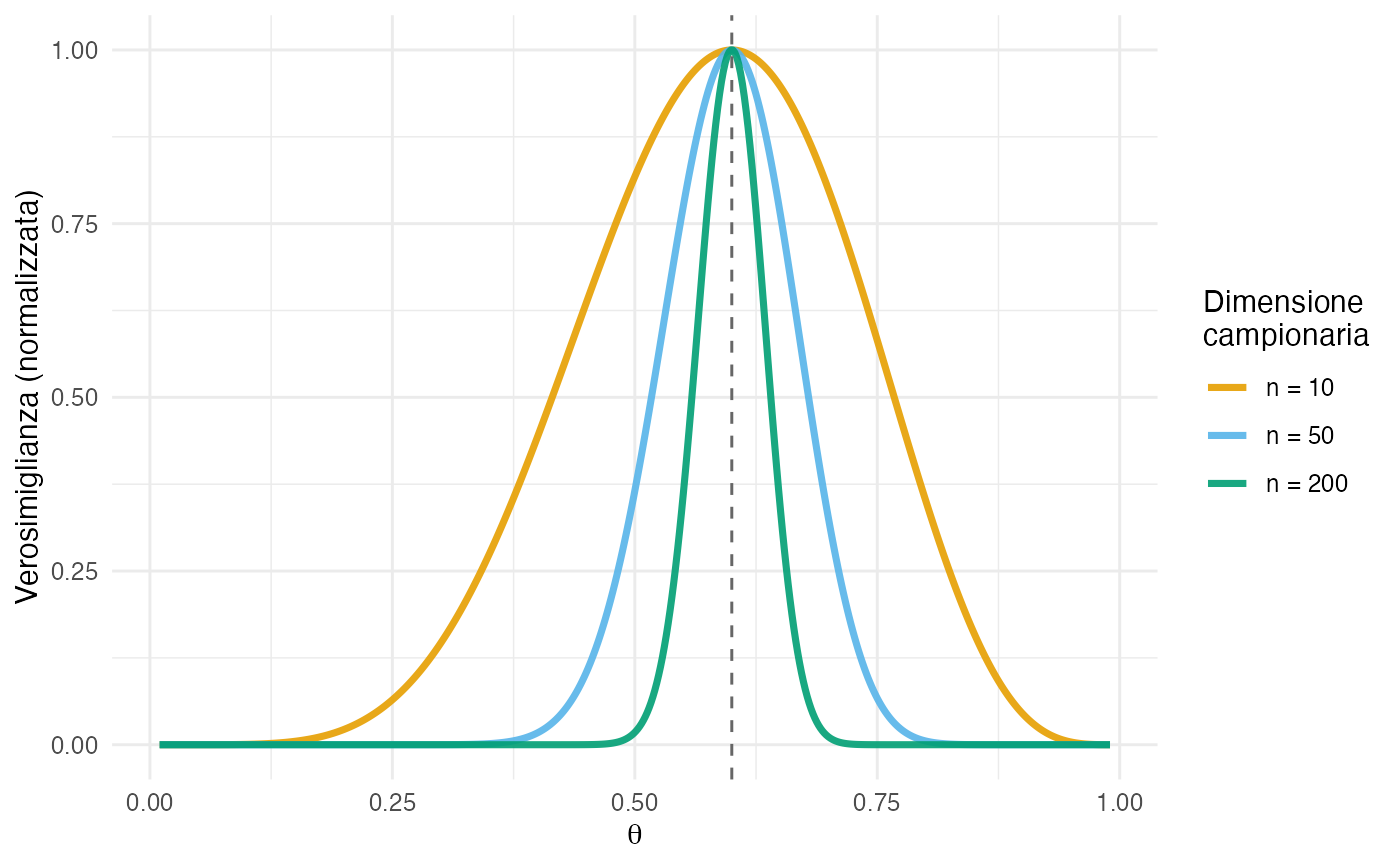
\includegraphics[width=0.85\linewidth,height=\textheight,keepaspectratio]{chapters/probability/15_properties_likelihood_files/figure-pdf/fig-likelihood-n-1.png}

}

\caption{\label{fig-likelihood-n}La verosimiglianza diventa più
concentrata all'aumentare della dimensione campionaria. Tutti i campioni
hanno la stessa proporzione osservata (0.6), ma la precisione aumenta
con n.}

\end{figure}%

Il grafico mostra chiaramente come la verosimiglianza si restringa
attorno al valore osservato \(\bar{X} = 0.6\) all'aumentare di \(n\).
Con \(n = 10\), molti valori di \(\theta\) sono ancora plausibili,
mentre con \(n = 200\), solo i valori molto vicini a 0.6 hanno una
verosimiglianza apprezzabile.

\section{Precisione e
informatività}\label{precisione-e-informativituxe0}

\subsection{La precisione come inverso della
varianza}\label{la-precisione-come-inverso-della-varianza}

Nell'inferenza bayesiana risulta particolarmente efficace ragionare in
termini di \textbf{precisione}, definita come l'inverso della varianza:
\[
\tau = \frac{1}{\sigma^2}.
\]

Questa definizione non è meramente formale: la precisione possiede
proprietà algebriche che rendono il meccanismo di aggiornamento
bayesiano particolarmente chiaro e lineare.

Applicando questo concetto alla media campionaria, otteniamo: \[
\text{Precisione}(\bar{X} \mid \theta) = \frac{1}{\text{Var}(\bar{X} \mid \theta)} = \frac{n}{\sigma^2}.
\]

\textbf{Osservazione fondamentale}: la precisione cresce in modo
\textbf{lineare} con il numero di osservazioni \(n\). Ciò significa che
ogni nuova osservazione aggiunge una quantità fissa di informazione,
indipendentemente dalla dimensione campionaria già raggiunta.

\subsection{L'errore standard come misura di
informatività}\label{lerrore-standard-come-misura-di-informativituxe0}

L'errore standard \(\text{SE} = \sigma/\sqrt{n}\) quantifica
l'incertezza della media campionaria come stimatore del parametro
\(\mu\), ovvero la media della popolazione. In termini bayesiani:

\begin{itemize}
\tightlist
\item
  un errore standard piccolo indica che i dati sono molto informativi,
  ovvero che la verosimiglianza è stretta e concentrata;
\item
  un errore standard grande indica che i dati sono poco informativi,
  ovvero che la verosimiglianza è ampia e dispersa.
\end{itemize}

\begin{Shaded}
\begin{Highlighting}[]
\NormalTok{n\_seq }\OtherTok{\textless{}{-}} \DecValTok{1}\SpecialCharTok{:}\DecValTok{200}
\NormalTok{sigma }\OtherTok{\textless{}{-}} \DecValTok{1}  \CommentTok{\# varianza unitaria per semplicità}

\NormalTok{precision\_data }\OtherTok{\textless{}{-}} \FunctionTok{data.frame}\NormalTok{(}
  \AttributeTok{n =}\NormalTok{ n\_seq,}
  \AttributeTok{se =}\NormalTok{ sigma }\SpecialCharTok{/} \FunctionTok{sqrt}\NormalTok{(n\_seq),}
  \AttributeTok{precision =}\NormalTok{ n\_seq }\SpecialCharTok{/}\NormalTok{ sigma}\SpecialCharTok{\^{}}\DecValTok{2}
\NormalTok{)}

\NormalTok{p1 }\OtherTok{\textless{}{-}} \FunctionTok{ggplot}\NormalTok{(precision\_data, }\FunctionTok{aes}\NormalTok{(}\AttributeTok{x =}\NormalTok{ n, }\AttributeTok{y =}\NormalTok{ se)) }\SpecialCharTok{+}
  \FunctionTok{geom\_line}\NormalTok{(}\AttributeTok{linewidth =} \FloatTok{1.2}\NormalTok{, }\AttributeTok{color =} \StringTok{"\#4E79A7"}\NormalTok{) }\SpecialCharTok{+}
  \FunctionTok{labs}\NormalTok{(}
    \AttributeTok{x =} \StringTok{"Dimensione campionaria (n)"}\NormalTok{,}
    \AttributeTok{y =} \StringTok{"Errore standard"}\NormalTok{,}
    \AttributeTok{title =} \StringTok{"Errore standard decresce come 1/√n"}
\NormalTok{  ) }\SpecialCharTok{+}
  \FunctionTok{theme\_minimal}\NormalTok{()}

\NormalTok{p2 }\OtherTok{\textless{}{-}} \FunctionTok{ggplot}\NormalTok{(precision\_data, }\FunctionTok{aes}\NormalTok{(}\AttributeTok{x =}\NormalTok{ n, }\AttributeTok{y =}\NormalTok{ precision)) }\SpecialCharTok{+}
  \FunctionTok{geom\_line}\NormalTok{(}\AttributeTok{linewidth =} \FloatTok{1.2}\NormalTok{, }\AttributeTok{color =} \StringTok{"\#E15759"}\NormalTok{) }\SpecialCharTok{+}
  \FunctionTok{labs}\NormalTok{(}
    \AttributeTok{x =} \StringTok{"Dimensione campionaria (n)"}\NormalTok{,}
    \AttributeTok{y =} \StringTok{"Precisione"}\NormalTok{,}
    \AttributeTok{title =} \StringTok{"Precisione cresce linearmente con n"}
\NormalTok{  ) }\SpecialCharTok{+}
  \FunctionTok{theme\_minimal}\NormalTok{()}

\NormalTok{p1 }\SpecialCharTok{+}\NormalTok{ p2}
\end{Highlighting}
\end{Shaded}

\begin{figure}[H]

\centering{

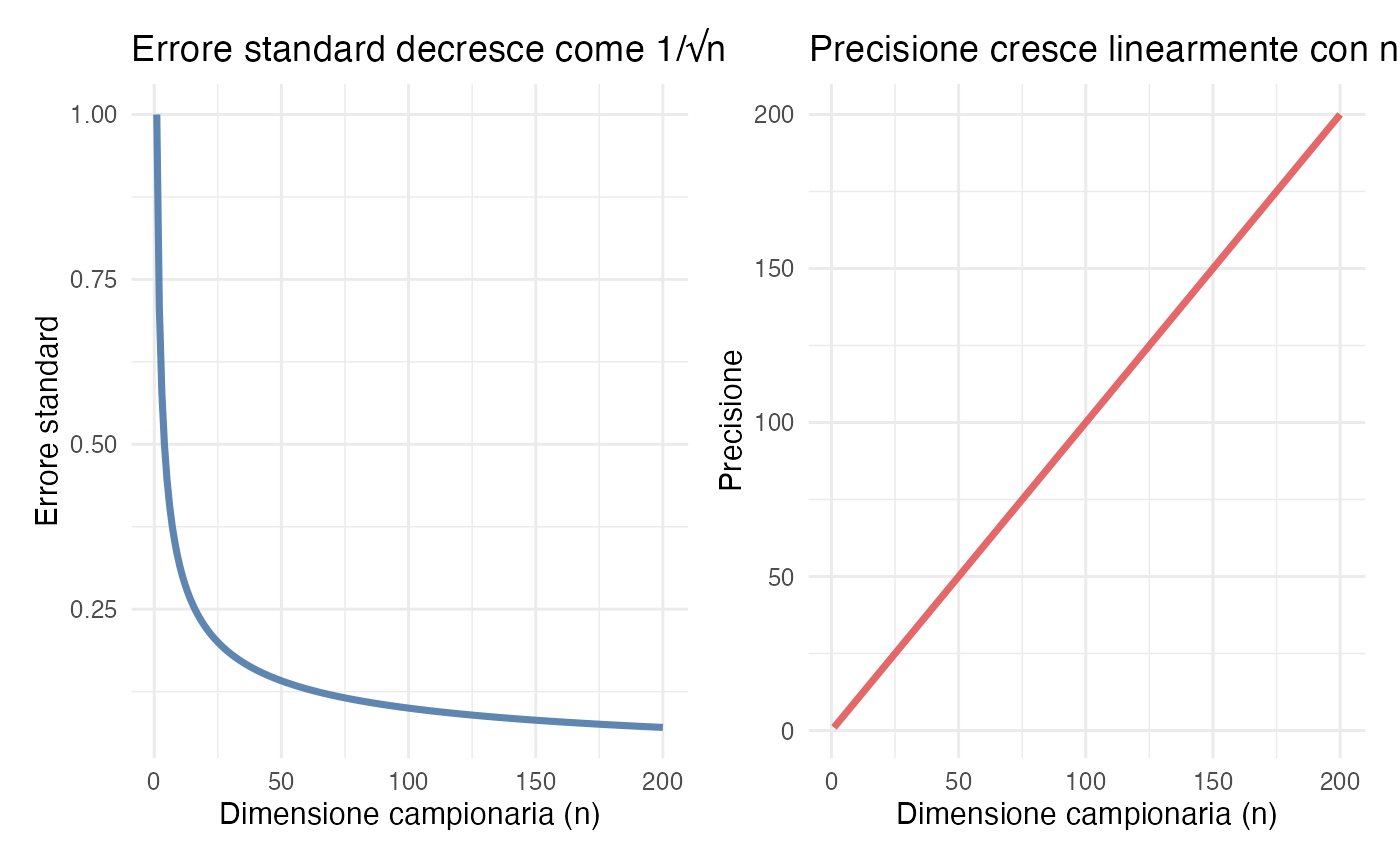
\includegraphics[width=0.85\linewidth,height=\textheight,keepaspectratio]{chapters/probability/15_properties_likelihood_files/figure-pdf/fig-precision-vs-n-1.png}

}

\caption{\label{fig-precision-vs-n}Relazione tra dimensione campionaria,
errore standard e precisione. Mentre l'errore standard decresce come
1/√n, la precisione cresce linearmente con n.}

\end{figure}%

\section{L'aggiornamento bayesiano come combinazione di
precisioni}\label{laggiornamento-bayesiano-come-combinazione-di-precisioni}

\subsection{Il caso gaussiano: una derivazione
esplicita}\label{il-caso-gaussiano-una-derivazione-esplicita}

Consideriamo il modello più semplice e rivelatore: osservazioni
distribuite normalmente con varianza nota. Supponiamo di avere una
credenza iniziale sul parametro \(\theta\), formalizzata da una
distribuzione a priori gaussiana,
\(\theta \sim \mathcal{N}(\mu_0, \sigma_0^2)\). Questo esprime la nostra
aspettativa che il valore \(\theta\) si trovi intorno a \(\mu_0\), con
un'incertezza quantificata da \(\sigma_0^2\).

A questo punto, si raccolgono i dati: \(n\) osservazioni indipendenti
\(X_1, ..., X_n\), ciascuna distribuita come
\(\mathcal{N}(\theta, \sigma^2)\), dove la varianza \(\sigma^2\) è nota.
L'informazione rilevante contenuta in questo campione è sintetizzata
dalla media campionaria \(\bar{X}\).

La verosimiglianza, ovvero la plausibilità dei diversi valori di
\(\theta\) alla luce dei dati osservati, assume una forma familiare.
Considerata come funzione di \(\theta\), essa è proporzionale a una
gaussiana: \[
L(\theta \mid \bar{x}) \propto \exp\left(-\frac{n(\bar{x} - \theta)^2}{2\sigma^2}\right).
\] Questa curva è centrata esattamente sulla media osservata \(\bar{x}\)
e ha una varianza pari a \(\sigma^2/n\), il che riflette il fatto che
l'incertezza sul valore effettivo di \(\theta\) diminuisce con
l'aumentare del numero di osservazioni.

\subsection{La distribuzione a
posteriori}\label{la-distribuzione-a-posteriori}

Il teorema di Bayes ci dice come combinare la nostra conoscenza iniziale
con la nuova evidenza: \[
p(\theta \mid \bar{x}) \propto p(\theta) \times L(\theta \mid \bar{x}).
\]

Nello specifico, il prodotto di due distribuzioni normali (il prior e la
verosimiglianza) genera una nuova distribuzione normale. Pertanto, la
nostra credenza aggiornata, o distribuzione a posteriori, sarà ancora
una gaussiana: \[
\theta \mid \bar{x} \sim \mathcal{N}(\mu_{\text{post}}, \sigma_{\text{post}}^2),
\] con una nuova media \(\mu_{\text{post}}\) e una nuova varianza
\(\sigma_{\text{post}}^2\).

\begin{theorem}[Aggiornamento bayesiano
gaussiano]\protect\hypertarget{thm-posterior-gaussian}{}\label{thm-posterior-gaussian}

I parametri di questa nuova distribuzione si calcolano nel modo
seguente. La \textbf{media a posteriori} \(\mu_{\text{post}}\) non è
altro che una media ponderata tra la nostra convinzione iniziale
\(\mu_0\) e l'evidenza dei dati \(\bar{x}\): \[
\mu_{\text{post}} = \frac{\tau_0 \mu_0 + \tau_{\text{dati}} \bar{x}}{\tau_0 + \tau_{\text{dati}}},
\] dove i pesi sono le rispettive \textbf{precisioni} (gli inversi delle
varianze): \(\tau_0 = 1/\sigma_0^2\) per il prior e
\(\tau_{\text{dati}} = n/\sigma^2\) per i dati.

Allo stesso modo, la \textbf{precisione a posteriori} --- che misura
quantitativamente la certezza della nostra stima aggiornata --- è
semplicemente la somma delle precisioni che abbiamo combinato: \[
\tau_{\text{post}} = \tau_0 + \tau_{\text{dati}}.
\]

\end{theorem}

\subsection{Interpretazione}\label{interpretazione-1}

Queste formule esprimono la logica profonda dell'aggiornamento
bayesiano:

\begin{enumerate}
\def\labelenumi{\arabic{enumi}.}
\item
  \textbf{Combinazione ponderata:} la media a posteriori è un
  compromesso tra la credenza iniziale (\(\mu_0\)) e l'evidenza empirica
  (\(\bar{x}\)), ponderato dalle rispettive precisioni. Un'informazione
  più precisa (maggiore \(\tau\)) riceve un peso maggiore nella stima
  finale.
\item
  \textbf{Accumulo di informazione:} la precisione a posteriori è sempre
  superiore sia alla precisione a priori che a quella dei dati presi
  separatamente. L'informazione si somma, riducendo l'incertezza
  complessiva.
\item
  \textbf{Dominanza dei dati:} quando \(n\) è grande,
  \(\tau_{\text{dati}}\) diventa molto elevata. In tal caso
  \(\mu_{\text{post}} \approx \bar{x}\) e la distribuzione a posteriori
  è determinata quasi esclusivamente dall'evidenza empirica.
\item
  \textbf{Dominanza del prior:} quando \(n\) è piccolo o i dati sono
  molto rumorosi (\(\sigma^2\) grande), \(\tau_{\text{dati}}\) è
  modesta. In questa situazione \(\mu_{\text{post}} \approx \mu_0\), e
  le credenze iniziali rimangono dominanti.
\end{enumerate}

\subsection{Esempio numerico}\label{esempio-numerico}

\begin{Shaded}
\begin{Highlighting}[]
\CommentTok{\# Parametri del prior}
\NormalTok{mu\_0 }\OtherTok{\textless{}{-}} \DecValTok{100}
\NormalTok{sigma\_0 }\OtherTok{\textless{}{-}} \DecValTok{15}
\NormalTok{tau\_0 }\OtherTok{\textless{}{-}} \DecValTok{1} \SpecialCharTok{/}\NormalTok{ sigma\_0}\SpecialCharTok{\^{}}\DecValTok{2}

\CommentTok{\# Parametri dei dati}
\NormalTok{n }\OtherTok{\textless{}{-}} \DecValTok{25}
\NormalTok{x\_bar }\OtherTok{\textless{}{-}} \DecValTok{115}
\NormalTok{sigma }\OtherTok{\textless{}{-}} \DecValTok{20}  \CommentTok{\# deviazione standard nota}
\NormalTok{tau\_data }\OtherTok{\textless{}{-}}\NormalTok{ n }\SpecialCharTok{/}\NormalTok{ sigma}\SpecialCharTok{\^{}}\DecValTok{2}

\CommentTok{\# Calcolo della posterior}
\NormalTok{tau\_post }\OtherTok{\textless{}{-}}\NormalTok{ tau\_0 }\SpecialCharTok{+}\NormalTok{ tau\_data}
\NormalTok{sigma\_post }\OtherTok{\textless{}{-}} \FunctionTok{sqrt}\NormalTok{(}\DecValTok{1} \SpecialCharTok{/}\NormalTok{ tau\_post)}
\NormalTok{mu\_post }\OtherTok{\textless{}{-}}\NormalTok{ (tau\_0 }\SpecialCharTok{*}\NormalTok{ mu\_0 }\SpecialCharTok{+}\NormalTok{ tau\_data }\SpecialCharTok{*}\NormalTok{ x\_bar) }\SpecialCharTok{/}\NormalTok{ tau\_post}

\CommentTok{\# Griglia di valori}
\NormalTok{theta\_grid }\OtherTok{\textless{}{-}} \FunctionTok{seq}\NormalTok{(}\DecValTok{60}\NormalTok{, }\DecValTok{150}\NormalTok{, }\AttributeTok{length.out =} \DecValTok{500}\NormalTok{)}

\CommentTok{\# Calcolo delle distribuzioni}
\NormalTok{prior\_density }\OtherTok{\textless{}{-}} \FunctionTok{dnorm}\NormalTok{(theta\_grid, mu\_0, sigma\_0)}
\NormalTok{likelihood }\OtherTok{\textless{}{-}} \FunctionTok{dnorm}\NormalTok{(theta\_grid, x\_bar, sigma }\SpecialCharTok{/} \FunctionTok{sqrt}\NormalTok{(n))}
\NormalTok{posterior\_density }\OtherTok{\textless{}{-}} \FunctionTok{dnorm}\NormalTok{(theta\_grid, mu\_post, sigma\_post)}

\CommentTok{\# Normalizzazione per visualizzazione}
\NormalTok{likelihood\_norm }\OtherTok{\textless{}{-}}\NormalTok{ likelihood }\SpecialCharTok{*} \FunctionTok{max}\NormalTok{(prior\_density) }\SpecialCharTok{/} \FunctionTok{max}\NormalTok{(likelihood)}

\NormalTok{plot\_data }\OtherTok{\textless{}{-}} \FunctionTok{data.frame}\NormalTok{(}
  \AttributeTok{theta =} \FunctionTok{rep}\NormalTok{(theta\_grid, }\DecValTok{3}\NormalTok{),}
  \AttributeTok{density =} \FunctionTok{c}\NormalTok{(prior\_density, likelihood\_norm, posterior\_density),}
  \AttributeTok{type =} \FunctionTok{factor}\NormalTok{(}\FunctionTok{rep}\NormalTok{(}\FunctionTok{c}\NormalTok{(}\StringTok{"Prior"}\NormalTok{, }\StringTok{"Verosimiglianza"}\NormalTok{, }\StringTok{"Posterior"}\NormalTok{), }\AttributeTok{each =} \FunctionTok{length}\NormalTok{(theta\_grid)),}
                \AttributeTok{levels =} \FunctionTok{c}\NormalTok{(}\StringTok{"Prior"}\NormalTok{, }\StringTok{"Verosimiglianza"}\NormalTok{, }\StringTok{"Posterior"}\NormalTok{))}
\NormalTok{)}

\FunctionTok{ggplot}\NormalTok{(plot\_data, }\FunctionTok{aes}\NormalTok{(}\AttributeTok{x =}\NormalTok{ theta, }\AttributeTok{y =}\NormalTok{ density, }\AttributeTok{color =}\NormalTok{ type, }\AttributeTok{linetype =}\NormalTok{ type)) }\SpecialCharTok{+}
  \FunctionTok{geom\_line}\NormalTok{(}\AttributeTok{linewidth =} \FloatTok{1.2}\NormalTok{) }\SpecialCharTok{+}
  \FunctionTok{scale\_color\_manual}\NormalTok{(}\AttributeTok{values =} \FunctionTok{c}\NormalTok{(}\StringTok{"\#4E79A7"}\NormalTok{, }\StringTok{"\#E69F00"}\NormalTok{, }\StringTok{"\#59A14F"}\NormalTok{)) }\SpecialCharTok{+}
  \FunctionTok{scale\_linetype\_manual}\NormalTok{(}\AttributeTok{values =} \FunctionTok{c}\NormalTok{(}\StringTok{"solid"}\NormalTok{, }\StringTok{"dashed"}\NormalTok{, }\StringTok{"solid"}\NormalTok{)) }\SpecialCharTok{+}
  \FunctionTok{labs}\NormalTok{(}
    \AttributeTok{x =} \FunctionTok{expression}\NormalTok{(theta),}
    \AttributeTok{y =} \StringTok{"Densità"}\NormalTok{,}
    \AttributeTok{color =} \StringTok{""}\NormalTok{,}
    \AttributeTok{linetype =} \StringTok{""}
\NormalTok{  ) }\SpecialCharTok{+}
  \FunctionTok{theme\_minimal}\NormalTok{() }
\end{Highlighting}
\end{Shaded}

\begin{figure}[H]

\centering{

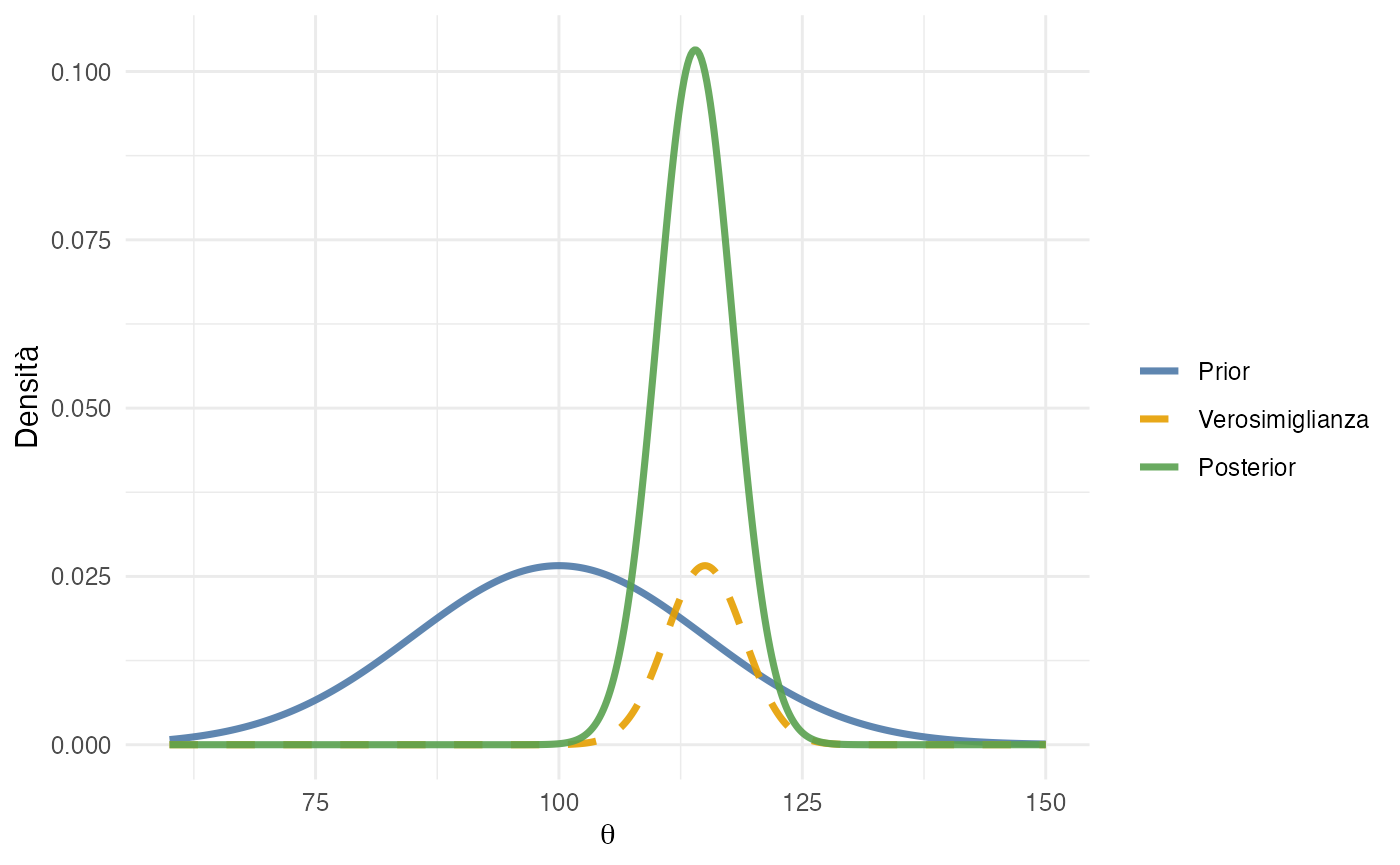
\includegraphics[width=0.85\linewidth,height=\textheight,keepaspectratio]{chapters/probability/15_properties_likelihood_files/figure-pdf/fig-bayesian-update-1.png}

}

\caption{\label{fig-bayesian-update}Aggiornamento bayesiano: il prior
(blu), la verosimiglianza (arancione) e la distribuzione a posteriori
(verde). La posterior è un compromesso tra prior e dati, pesato dalle
rispettive precisioni.}

\end{figure}%

\begin{Shaded}
\begin{Highlighting}[]
\CommentTok{\# Stampa dei risultati}
\FunctionTok{cat}\NormalTok{(}\StringTok{"Prior: N("}\NormalTok{, mu\_0, }\StringTok{", "}\NormalTok{, sigma\_0, }\StringTok{"²)}\SpecialCharTok{\textbackslash{}n}\StringTok{"}\NormalTok{, }\AttributeTok{sep =} \StringTok{""}\NormalTok{)}
\CommentTok{\#\textgreater{} Prior: N(100, 15²)}
\FunctionTok{cat}\NormalTok{(}\StringTok{"Dati: n ="}\NormalTok{, n, }\StringTok{", media campionaria ="}\NormalTok{, x\_bar, }\StringTok{"}\SpecialCharTok{\textbackslash{}n}\StringTok{"}\NormalTok{)}
\CommentTok{\#\textgreater{} Dati: n = 25 , media campionaria = 115}
\FunctionTok{cat}\NormalTok{(}\StringTok{"Precisione prior:"}\NormalTok{, }\FunctionTok{round}\NormalTok{(tau\_0, }\DecValTok{6}\NormalTok{), }\StringTok{"}\SpecialCharTok{\textbackslash{}n}\StringTok{"}\NormalTok{)}
\CommentTok{\#\textgreater{} Precisione prior: 0.00444}
\FunctionTok{cat}\NormalTok{(}\StringTok{"Precisione dati:"}\NormalTok{, }\FunctionTok{round}\NormalTok{(tau\_data, }\DecValTok{6}\NormalTok{), }\StringTok{"}\SpecialCharTok{\textbackslash{}n}\StringTok{"}\NormalTok{)}
\CommentTok{\#\textgreater{} Precisione dati: 0.0625}
\FunctionTok{cat}\NormalTok{(}\StringTok{"Precisione posterior:"}\NormalTok{, }\FunctionTok{round}\NormalTok{(tau\_post, }\DecValTok{6}\NormalTok{), }\StringTok{"}\SpecialCharTok{\textbackslash{}n}\StringTok{"}\NormalTok{)}
\CommentTok{\#\textgreater{} Precisione posterior: 0.0669}
\FunctionTok{cat}\NormalTok{(}\StringTok{"}\SpecialCharTok{\textbackslash{}n}\StringTok{Media posterior:"}\NormalTok{, }\FunctionTok{round}\NormalTok{(mu\_post, }\DecValTok{2}\NormalTok{), }\StringTok{"}\SpecialCharTok{\textbackslash{}n}\StringTok{"}\NormalTok{)}
\CommentTok{\#\textgreater{} }
\CommentTok{\#\textgreater{} Media posterior: 114}
\FunctionTok{cat}\NormalTok{(}\StringTok{"Deviazione standard posterior:"}\NormalTok{, }\FunctionTok{round}\NormalTok{(sigma\_post, }\DecValTok{2}\NormalTok{), }\StringTok{"}\SpecialCharTok{\textbackslash{}n}\StringTok{"}\NormalTok{)}
\CommentTok{\#\textgreater{} Deviazione standard posterior: 3.86}
\end{Highlighting}
\end{Shaded}

\begin{tcolorbox}[enhanced jigsaw, arc=.35mm, breakable, colbacktitle=quarto-callout-note-color!10!white, opacityback=0, toprule=.15mm, rightrule=.15mm, colback=white, opacitybacktitle=0.6, leftrule=.75mm, coltitle=black, bottomtitle=1mm, left=2mm, toptitle=1mm, title=\textcolor{quarto-callout-note-color}{\faInfo}\hspace{0.5em}{Il peso relativo di prior e dati}, titlerule=0mm, bottomrule=.15mm, colframe=quarto-callout-note-color-frame]

In questo esempio, la precisione dei dati
(\(\tau_{\text{dati}} = 0.062\)) è circa 14.1 volte maggiore della
precisione del prior (\(\tau_0 = 0.004\)). Di conseguenza, la media a
posteriori (114) è molto più vicina alla media campionaria (115) che
alla media a priori (100).

\end{tcolorbox}

\section{La Legge dei Grandi Numeri e la convergenza
bayesiana}\label{la-legge-dei-grandi-numeri-e-la-convergenza-bayesiana}

Tra i risultati fondamentali della teoria della probabilità, la
\textbf{Legge dei Grandi Numeri (LGN)} descrive come l'informazione
fornita dai dati tenda a stabilizzarsi con l'aumentare delle
osservazioni. Nella sua interpretazione più intuitiva, essa afferma che,
ripetendo molte volte un esperimento nelle stesse condizioni, la
frequenza relativa di un evento si avvicina sempre di più alla sua
probabilità teorica.

Formalmente, se \(X_1, \dots, X_n\) sono variabili aleatorie
indipendenti e identicamente distribuite con valore atteso \(\mu\), la
media campionaria

\[
\bar X_n = \frac{1}{n}\sum_{i=1}^{n} X_i
\] tende, al crescere di \(n\), a concentrarsi attorno alla quantità
costante \(\mu\). Questa convergenza non significa che gli scarti dal
valore vero scompaiono, ma che diventano \textbf{sempre meno probabili}:
la media può ancora fluttuare, ma tali oscillazioni risulteranno via via
più contenute e statisticamente trascurabili rispetto a \(\mu\).

\subsection{Conseguenze per la
verosimiglianza}\label{conseguenze-per-la-verosimiglianza}

La LGN esercita un'influenza diretta sulla funzione di verosimiglianza,
poiché ne determina il comportamento asintotico. Quando lo stimatore di
massima verosimiglianza coincide con una statistica campionaria --- come
accade per la media nei modelli gaussiani --- esso converge al valore
vero del parametro. Di conseguenza, la verosimiglianza concentra
progressivamente tutta la propria massa attorno a tale valore,
restringendo lo spazio dei parametri plausibili. L'accumularsi dei dati
non elimina l'incertezza, ma la rende sempre più localizzata: le
alternative al valore corretto non scompaiono, ma diventano via via meno
credibili fino a risultare statisticamente trascurabili.

\subsection{Conseguenze per l'inferenza bayesiana:
consistenza}\label{conseguenze-per-linferenza-bayesiana-consistenza}

Questo comportamento si riflette in modo naturale sull'aggiornamento
delle credenze nell'ambito bayesiano, dando luogo al principio della
\textbf{consistenza bayesiana}.

\begin{theorem}[Consistenza
bayesiana]\protect\hypertarget{thm-bayesian-consistency}{}\label{thm-bayesian-consistency}

Se la distribuzione a priori assegna probabilità positiva a ogni intorno
del valore vero \(\theta_0\), allora, quando \(n \to \infty\), la
distribuzione a posteriori converge a una distribuzione degenerata
concentrata interamente in \(\theta_0\).

\end{theorem}

La rilevanza di questo risultato è concettuale oltre che operativa.
L'inferenza bayesiana si presenta come un procedimento
\textbf{auto-correttivo}: qualsiasi prior a supporto positivo --- cioè
che non escluda a priori il valore vero --- conduce alle stesse
conclusioni quando l'evidenza empirica diventa sufficientemente ricca.
Le credenze iniziali possono essere imprecise o addirittura fuorvianti,
ma l'accumulo dei dati le spinge gradualmente verso la realtà, rendendo
l'analisi sempre più dominata dall'informazione proveniente dai dati
stessi. Al crescere della dimensione del campione, la distribuzione a
posteriori diventa quindi una rappresentazione sempre più accurata e
concentrata del parametro che governa il fenomeno in esame.

\subsection{Simulazione: convergenza con prior
diversi}\label{simulazione-convergenza-con-prior-diversi}

\begin{Shaded}
\begin{Highlighting}[]
\FunctionTok{set.seed}\NormalTok{(}\DecValTok{42}\NormalTok{)}
\NormalTok{theta\_true }\OtherTok{\textless{}{-}} \FloatTok{0.45}
\NormalTok{n\_values }\OtherTok{\textless{}{-}} \FunctionTok{c}\NormalTok{(}\DecValTok{10}\NormalTok{, }\DecValTok{50}\NormalTok{, }\DecValTok{200}\NormalTok{, }\DecValTok{1000}\NormalTok{)}

\CommentTok{\# Prior diversi}
\NormalTok{priors }\OtherTok{\textless{}{-}} \FunctionTok{list}\NormalTok{(}
  \AttributeTok{A =} \FunctionTok{c}\NormalTok{(}\DecValTok{2}\NormalTok{, }\DecValTok{8}\NormalTok{),   }\CommentTok{\# Prior pessimista (media = 0.2)}
  \AttributeTok{B =} \FunctionTok{c}\NormalTok{(}\DecValTok{8}\NormalTok{, }\DecValTok{2}\NormalTok{),   }\CommentTok{\# Prior ottimista (media = 0.8)}
  \AttributeTok{C =} \FunctionTok{c}\NormalTok{(}\DecValTok{1}\NormalTok{, }\DecValTok{1}\NormalTok{)    }\CommentTok{\# Prior uniforme (media = 0.5)}
\NormalTok{)}

\CommentTok{\# Funzione per calcolare la posterior Beta}
\NormalTok{compute\_posterior }\OtherTok{\textless{}{-}} \ControlFlowTok{function}\NormalTok{(prior\_params, n, theta\_true) \{}
\NormalTok{  y }\OtherTok{\textless{}{-}} \FunctionTok{rbinom}\NormalTok{(}\DecValTok{1}\NormalTok{, n, theta\_true)}
  \FunctionTok{c}\NormalTok{(prior\_params[}\DecValTok{1}\NormalTok{] }\SpecialCharTok{+}\NormalTok{ y, prior\_params[}\DecValTok{2}\NormalTok{] }\SpecialCharTok{+}\NormalTok{ n }\SpecialCharTok{{-}}\NormalTok{ y)}
\NormalTok{\}}

\CommentTok{\# Generazione dei dati per il plot}
\FunctionTok{set.seed}\NormalTok{(}\DecValTok{42}\NormalTok{)}
\NormalTok{theta\_grid }\OtherTok{\textless{}{-}} \FunctionTok{seq}\NormalTok{(}\FloatTok{0.01}\NormalTok{, }\FloatTok{0.99}\NormalTok{, }\AttributeTok{length.out =} \DecValTok{300}\NormalTok{)}

\NormalTok{all\_data }\OtherTok{\textless{}{-}} \FunctionTok{do.call}\NormalTok{(rbind, }\FunctionTok{lapply}\NormalTok{(n\_values, }\ControlFlowTok{function}\NormalTok{(n) \{}
  \FunctionTok{do.call}\NormalTok{(rbind, }\FunctionTok{lapply}\NormalTok{(}\FunctionTok{names}\NormalTok{(priors), }\ControlFlowTok{function}\NormalTok{(name) \{}
\NormalTok{    post }\OtherTok{\textless{}{-}} \FunctionTok{compute\_posterior}\NormalTok{(priors[[name]], n, theta\_true)}
    \FunctionTok{data.frame}\NormalTok{(}
      \AttributeTok{theta =}\NormalTok{ theta\_grid,}
      \AttributeTok{density =} \FunctionTok{dbeta}\NormalTok{(theta\_grid, post[}\DecValTok{1}\NormalTok{], post[}\DecValTok{2}\NormalTok{]),}
      \AttributeTok{researcher =}\NormalTok{ name,}
      \AttributeTok{n =}\NormalTok{ n}
\NormalTok{    )}
\NormalTok{  \}))}
\NormalTok{\}))}

\NormalTok{all\_data}\SpecialCharTok{$}\NormalTok{n\_label }\OtherTok{\textless{}{-}} \FunctionTok{factor}\NormalTok{(}\FunctionTok{paste}\NormalTok{(}\StringTok{"n ="}\NormalTok{, all\_data}\SpecialCharTok{$}\NormalTok{n), }
                           \AttributeTok{levels =} \FunctionTok{paste}\NormalTok{(}\StringTok{"n ="}\NormalTok{, n\_values))}
\NormalTok{all\_data}\SpecialCharTok{$}\NormalTok{researcher }\OtherTok{\textless{}{-}} \FunctionTok{factor}\NormalTok{(all\_data}\SpecialCharTok{$}\NormalTok{researcher,}
                              \AttributeTok{labels =} \FunctionTok{c}\NormalTok{(}\StringTok{"Prior pessimista (β = 0.2)"}\NormalTok{,}
                                        \StringTok{"Prior ottimista (β = 0.8)"}\NormalTok{, }
                                        \StringTok{"Prior uniforme"}\NormalTok{))}

\FunctionTok{ggplot}\NormalTok{(all\_data, }\FunctionTok{aes}\NormalTok{(}\AttributeTok{x =}\NormalTok{ theta, }\AttributeTok{y =}\NormalTok{ density, }\AttributeTok{color =}\NormalTok{ researcher)) }\SpecialCharTok{+}
  \FunctionTok{geom\_line}\NormalTok{(}\AttributeTok{linewidth =} \DecValTok{1}\NormalTok{) }\SpecialCharTok{+}
  \FunctionTok{geom\_vline}\NormalTok{(}\AttributeTok{xintercept =}\NormalTok{ theta\_true, }\AttributeTok{linetype =} \StringTok{"dashed"}\NormalTok{, }
             \AttributeTok{color =} \StringTok{"gray40"}\NormalTok{, }\AttributeTok{linewidth =} \FloatTok{0.8}\NormalTok{) }\SpecialCharTok{+}
  \FunctionTok{facet\_wrap}\NormalTok{(}\SpecialCharTok{\textasciitilde{}}\NormalTok{ n\_label, }\AttributeTok{scales =} \StringTok{"free\_y"}\NormalTok{, }\AttributeTok{ncol =} \DecValTok{2}\NormalTok{) }\SpecialCharTok{+}
  \FunctionTok{scale\_color\_manual}\NormalTok{(}\AttributeTok{values =} \FunctionTok{c}\NormalTok{(}\StringTok{"\#4E79A7"}\NormalTok{, }\StringTok{"\#E15759"}\NormalTok{, }\StringTok{"\#59A14F"}\NormalTok{)) }\SpecialCharTok{+}
  \FunctionTok{labs}\NormalTok{(}
    \AttributeTok{x =} \FunctionTok{expression}\NormalTok{(theta),}
    \AttributeTok{y =} \StringTok{"Densità a posteriori"}\NormalTok{,}
    \AttributeTok{color =} \StringTok{"Ricercatore"}
\NormalTok{  ) }\SpecialCharTok{+}
  \FunctionTok{theme\_minimal}\NormalTok{() }\SpecialCharTok{+}
  \FunctionTok{theme}\NormalTok{(}\AttributeTok{legend.position =} \StringTok{"bottom"}\NormalTok{)}
\end{Highlighting}
\end{Shaded}

\begin{figure}[H]

\centering{

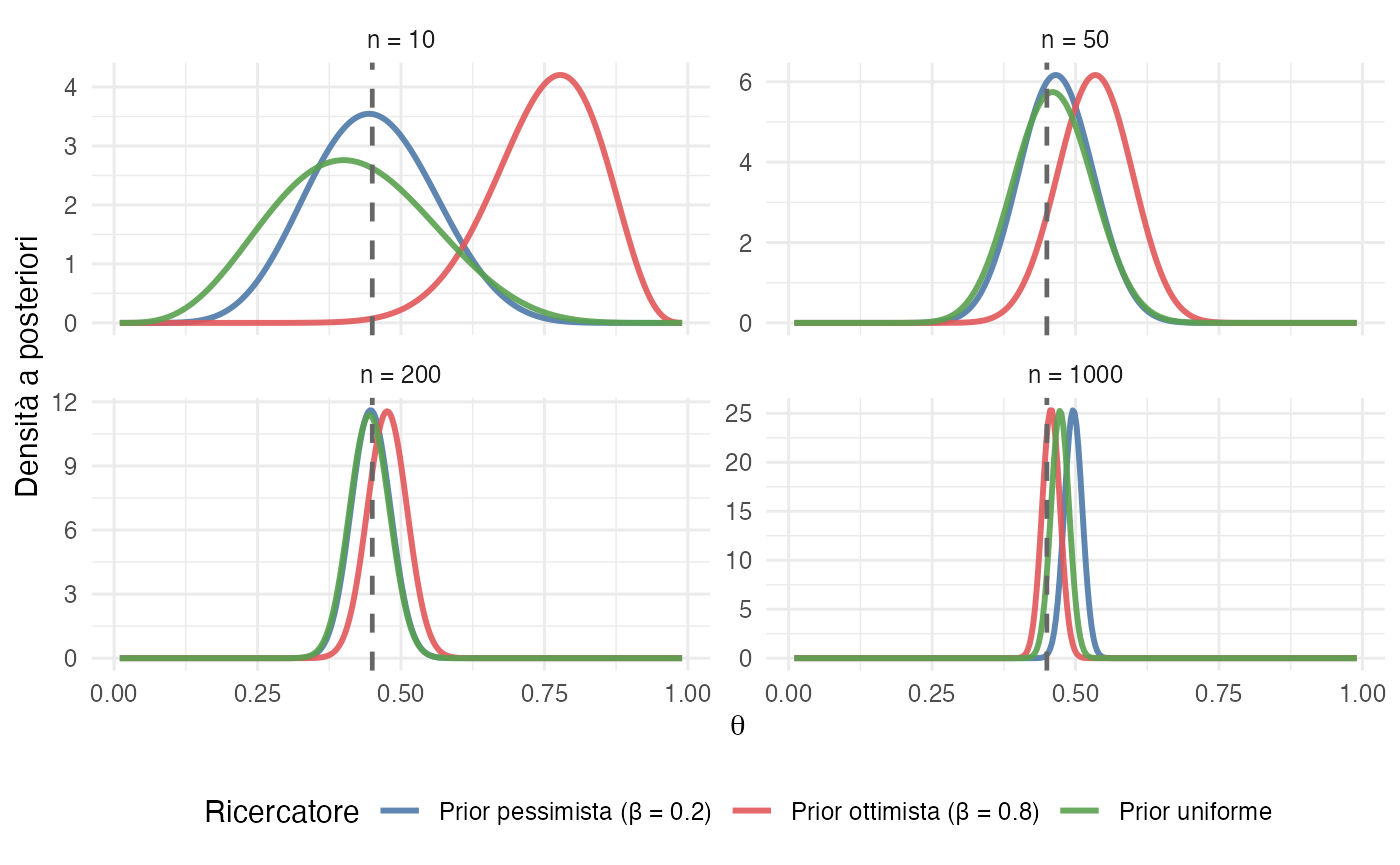
\includegraphics[width=0.85\linewidth,height=\textheight,keepaspectratio]{chapters/probability/15_properties_likelihood_files/figure-pdf/fig-convergence-1.png}

}

\caption{\label{fig-convergence}Convergenza bayesiana: tre ricercatori
con prior molto diversi convergono alla stessa conclusione all'aumentare
dei dati. La linea verticale indica il valore vero θ₀ = 0.45.}

\end{figure}%

\textbf{Osservazioni.} Con un campione ridotto di \(n = 10\) unità, le
distribuzioni a posteriori rimangono nettamente diverse tra loro,
riflettendo ancora fortemente l'influenza delle diverse credenze
iniziali. Con l'aumentare della dimensione del campione, con \(n = 50\)
si inizia a osservare un chiaro avvicinamento. Quando si raggiungono
\(n = 200\) osservazioni, le distribuzioni sono sostanzialmente
sovrapposte, il che indica che l'evidenza empirica sta prevalendo.
Infine, con \(n = 1000\) le distribuzioni a posteriori sono praticamente
indistinguibili e tutte fortemente concentrate attorno al valore vero
del parametro, a dimostrazione della proprietà di consistenza
dell'inferenza bayesiana.

\section{Il Teorema del Limite Centrale e l'approssimazione
normale}\label{il-teorema-del-limite-centrale-e-lapprossimazione-normale}

\subsection{Enunciato del Teorema del Limite
Centrale}\label{enunciato-del-teorema-del-limite-centrale}

Il \textbf{Teorema del Limite Centrale (TLC)} è un raffinamento della
legge dei grandi numeri che rende più precisa la convergenza delle medie
empiriche. Esso afferma che, indipendentemente dalla forma della
distribuzione delle singole osservazioni, la media campionaria tende a
una distribuzione normale.

\begin{theorem}[Teorema del Limite
Centrale]\protect\hypertarget{thm-clt}{}\label{thm-clt}

Per osservazioni i.i.d. con \(\mathbb{E}[X_i] = \mu\) e
\(\mathrm{Var}(X_i) = \sigma^2 < \infty\), \[
\bar{X}_n \;\dot\sim\; \mathcal{N}\!\left(\mu, \frac{\sigma^2}{n}\right) \qquad \text{per } n \text{ sufficientemente grande}.
\]

\end{theorem}

Questo risultato di ``universalità'' delle densità gaussiane fornisce
quindi una giustificazione della loro applicazione così diffusa in
molteplici ambiti.

\subsection{Conseguenza per la
verosimiglianza}\label{conseguenza-per-la-verosimiglianza}

Poiché la verosimiglianza spesso dipende dalla media campionaria, il TLC
implica che, per campioni sufficientemente ampi, essa assuma una forma
\textbf{approssimativamente normale} rispetto al parametro: \[
L(\theta \mid \bar{x}) \;\approx\; \mathcal{N}\!\left(\bar{x}, \frac{\sigma^2}{n}\right)
\qquad \text{interpretata come funzione di } \theta.
\]

Questa gaussianità non deriva dalla distribuzione delle singole
osservazioni, ma dal comportamento aggregato delle loro medie. Anche
quando i dati provengono da popolazioni con forme molto diverse dalla
normale, la verosimiglianza tende a seguire una struttura gaussiana: la
normalità emerge \emph{dal campionamento}, non dalla popolazione di
origine.

\subsection{Conseguenza per l'inferenza bayesiana: il teorema di
Bernstein--von
Mises}\label{conseguenza-per-linferenza-bayesiana-il-teorema-di-bernsteinvon-mises}

L'approssimazione normale della verosimiglianza si propaga in modo
diretto alla distribuzione a posteriori, dando luogo a un risultato
centrale della teoria bayesiana.

\begin{theorem}[Teorema di Bernstein--von
Mises]\protect\hypertarget{thm-bvm}{}\label{thm-bvm}

Sotto condizioni di regolarità, per campioni sufficientemente grandi, la
distribuzione a posteriori può essere approssimata accuratamente da una
distribuzione normale: \[
p(\theta \mid X_1, \ldots, X_n) \approx \mathcal{N}(\hat{\theta}_n,\, I_n^{-1}),
\] dove \(\hat{\theta}_n\) è lo stimatore di massima verosimiglianza e
\(I_n\) rappresenta l'\emph{informazione di Fisher} osservata, che
misura la quantità di informazione sul parametro contenuta nel campione.

\end{theorem}

\textbf{Interpretazione pratica.} La conseguenza principale è di natura
computazionale. Grazie all'approssimazione normale, il calcolo della
distribuzione a posteriori, che spesso è complesso o addirittura
intrattabile, può essere sostituito da formule approssimate più
semplici, anche in modelli non gaussiani. Questa semplificazione
consente di applicare l'inferenza bayesiana a una vasta gamma di
problemi, anche quando i modelli sottostanti non sono trattabili
analiticamente.

\subsection{Visualizzazione: il TLC in una popolazione non
normale}\label{visualizzazione-il-tlc-in-una-popolazione-non-normale}

\begin{Shaded}
\begin{Highlighting}[]
\FunctionTok{set.seed}\NormalTok{(}\DecValTok{42}\NormalTok{)}

\CommentTok{\# Popolazione: distribuzione uniforme (non gaussiana)}
\NormalTok{population }\OtherTok{\textless{}{-}} \FunctionTok{runif}\NormalTok{(}\FloatTok{1e6}\NormalTok{, }\AttributeTok{min =} \DecValTok{0}\NormalTok{, }\AttributeTok{max =} \DecValTok{1}\NormalTok{)}

\CommentTok{\# Funzione per simulare distribuzioni campionarie}
\NormalTok{simulate\_sampling\_dist }\OtherTok{\textless{}{-}} \ControlFlowTok{function}\NormalTok{(pop, sample\_size, }\AttributeTok{n\_samples =} \FloatTok{1e5}\NormalTok{) \{}
  \FunctionTok{replicate}\NormalTok{(n\_samples, }\FunctionTok{mean}\NormalTok{(}\FunctionTok{sample}\NormalTok{(pop, sample\_size, }\AttributeTok{replace =} \ConstantTok{TRUE}\NormalTok{)))}
\NormalTok{\}}

\CommentTok{\# Diverse dimensioni campionarie}
\NormalTok{sample\_sizes }\OtherTok{\textless{}{-}} \FunctionTok{c}\NormalTok{(}\DecValTok{1}\NormalTok{, }\DecValTok{5}\NormalTok{, }\DecValTok{30}\NormalTok{)}

\NormalTok{sampling\_data }\OtherTok{\textless{}{-}} \FunctionTok{do.call}\NormalTok{(rbind, }\FunctionTok{lapply}\NormalTok{(sample\_sizes, }\ControlFlowTok{function}\NormalTok{(n) \{}
\NormalTok{  means }\OtherTok{\textless{}{-}} \FunctionTok{simulate\_sampling\_dist}\NormalTok{(population, n)}
  \FunctionTok{data.frame}\NormalTok{(}
    \AttributeTok{mean =}\NormalTok{ means,}
    \AttributeTok{n =} \FunctionTok{factor}\NormalTok{(}\FunctionTok{paste}\NormalTok{(}\StringTok{"n ="}\NormalTok{, n), }\AttributeTok{levels =} \FunctionTok{paste}\NormalTok{(}\StringTok{"n ="}\NormalTok{, sample\_sizes))}
\NormalTok{  )}
\NormalTok{\}))}

\FunctionTok{ggplot}\NormalTok{(sampling\_data, }\FunctionTok{aes}\NormalTok{(}\AttributeTok{x =}\NormalTok{ mean)) }\SpecialCharTok{+}
  \FunctionTok{geom\_histogram}\NormalTok{(}\FunctionTok{aes}\NormalTok{(}\AttributeTok{y =} \FunctionTok{after\_stat}\NormalTok{(density)), }\AttributeTok{bins =} \DecValTok{40}\NormalTok{, }
                 \AttributeTok{fill =} \StringTok{"\#4E79A7"}\NormalTok{, }\AttributeTok{alpha =} \FloatTok{0.7}\NormalTok{) }\SpecialCharTok{+}
  \FunctionTok{stat\_function}\NormalTok{(}\AttributeTok{fun =}\NormalTok{ dnorm, }
                \AttributeTok{args =} \FunctionTok{list}\NormalTok{(}\AttributeTok{mean =} \FloatTok{0.5}\NormalTok{, }\AttributeTok{sd =} \FunctionTok{sqrt}\NormalTok{(}\DecValTok{1}\SpecialCharTok{/}\DecValTok{12}\NormalTok{) }\SpecialCharTok{/} \FunctionTok{sqrt}\NormalTok{(}\DecValTok{30}\NormalTok{)),}
                \AttributeTok{data =} \FunctionTok{subset}\NormalTok{(sampling\_data, n }\SpecialCharTok{==} \StringTok{"n = 30"}\NormalTok{),}
                \AttributeTok{color =} \StringTok{"\#E15759"}\NormalTok{, }\AttributeTok{linewidth =} \FloatTok{1.2}\NormalTok{) }\SpecialCharTok{+}
  \FunctionTok{facet\_wrap}\NormalTok{(}\SpecialCharTok{\textasciitilde{}}\NormalTok{ n, }\AttributeTok{scales =} \StringTok{"free\_y"}\NormalTok{) }\SpecialCharTok{+}
  \FunctionTok{labs}\NormalTok{(}
    \AttributeTok{x =} \StringTok{"Media campionaria"}\NormalTok{,}
    \AttributeTok{y =} \StringTok{"Densità"}
\NormalTok{  ) }\SpecialCharTok{+}
  \FunctionTok{theme\_minimal}\NormalTok{()}
\end{Highlighting}
\end{Shaded}

\begin{figure}[H]

\centering{

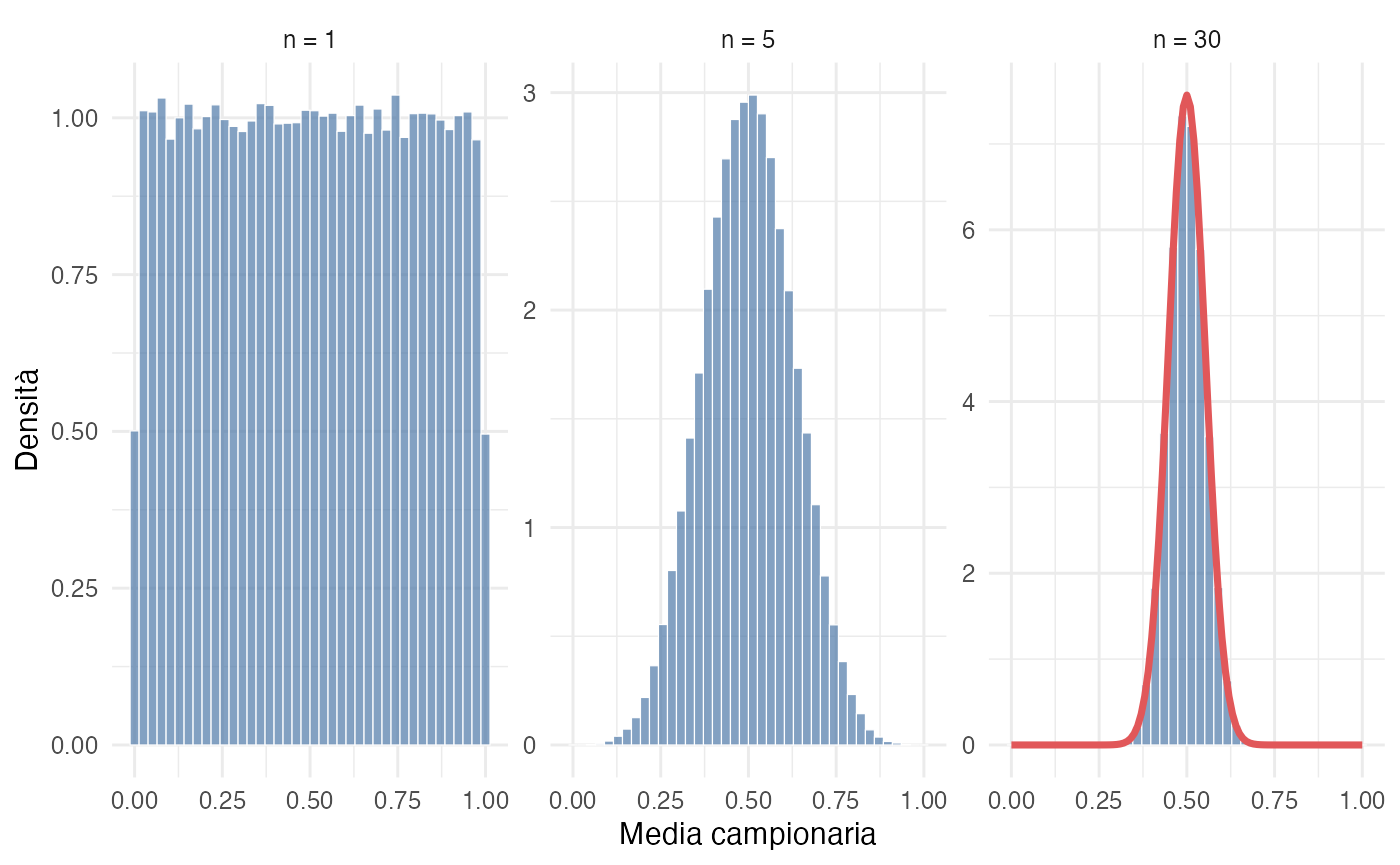
\includegraphics[width=0.85\linewidth,height=\textheight,keepaspectratio]{chapters/probability/15_properties_likelihood_files/figure-pdf/fig-clt-1.png}

}

\caption{\label{fig-clt}Il Teorema del Limite Centrale in azione: anche
partendo da una distribuzione uniforme, la distribuzione delle medie
campionarie converge rapidamente a una forma gaussiana.}

\end{figure}%

Con un solo dato (\(n = 1\)), la distribuzione delle ``medie
campionarie'' è semplicemente la distribuzione uniforme originale da cui
i dati sono tratti. Già con \(n = 5\) osservazioni, inizia a delinearsi
una forma a campana. Quando si arriva a \(n = 30\), la distribuzione
diventa praticamente indistinguibile da una curva normale, offrendo una
dimostrazione visiva immediata dell'universalità del TLC.

\section{Combinazione di evidenze da studi
multipli}\label{combinazione-di-evidenze-da-studi-multipli}

\subsection{Il principio della somma delle
precisioni}\label{il-principio-della-somma-delle-precisioni}

Una delle applicazioni più eleganti dell'approccio bayesiano è la
\textbf{sintesi di evidenze} provenienti da studi indipendenti. Quando
più ricerche indagano lo stesso parametro \(\theta\), le loro
informazioni possono essere combinate in modo naturale e coerente.

Se ciascuno studio \(i\) fornisce una stima \(\bar{x}_i\) con una
corrispondente precisione \(\tau_i\) (l'inverso della sua varianza), la
stima combinata risulta essere una \textbf{media ponderata}: \[
\bar{x}_{\text{comb}} = \frac{\sum_i \tau_i \bar{x}_i}{\sum_i \tau_i},
\] dove i pesi sono proprio le precisioni individuali. La precisione
totale della stima sintetica è semplicemente la somma delle precisioni
degli studi: \[
\tau_{\text{comb}} = \sum_i \tau_i.
\]

\subsection{Esempio: sintesi di due
studi}\label{esempio-sintesi-di-due-studi}

Consideriamo due studi indipendenti che stimano la prevalenza di un
sintomo:

\begin{Shaded}
\begin{Highlighting}[]
\CommentTok{\# Parametri degli studi}
\NormalTok{studi }\OtherTok{\textless{}{-}} \FunctionTok{data.frame}\NormalTok{(}
  \AttributeTok{studio =} \FunctionTok{c}\NormalTok{(}\StringTok{"A"}\NormalTok{, }\StringTok{"B"}\NormalTok{),}
  \AttributeTok{n =} \FunctionTok{c}\NormalTok{(}\DecValTok{50}\NormalTok{, }\DecValTok{200}\NormalTok{),}
  \AttributeTok{proporzione =} \FunctionTok{c}\NormalTok{(}\FloatTok{0.42}\NormalTok{, }\FloatTok{0.38}\NormalTok{),}
  \AttributeTok{se =} \FunctionTok{c}\NormalTok{(}\FloatTok{0.07}\NormalTok{, }\FloatTok{0.035}\NormalTok{)  }\CommentTok{\# Errore standard}
\NormalTok{)}

\CommentTok{\# Calcolo delle precisioni (inverso della varianza)}
\NormalTok{studi}\SpecialCharTok{$}\NormalTok{precisione }\OtherTok{\textless{}{-}} \DecValTok{1} \SpecialCharTok{/}\NormalTok{ studi}\SpecialCharTok{$}\NormalTok{se}\SpecialCharTok{\^{}}\DecValTok{2}

\CommentTok{\# Sintesi bayesiana (combinazione delle normali)}
\NormalTok{precisione\_totale }\OtherTok{\textless{}{-}} \FunctionTok{sum}\NormalTok{(studi}\SpecialCharTok{$}\NormalTok{precisione)}
\NormalTok{media\_combinata }\OtherTok{\textless{}{-}} \FunctionTok{sum}\NormalTok{(studi}\SpecialCharTok{$}\NormalTok{precisione }\SpecialCharTok{*}\NormalTok{ studi}\SpecialCharTok{$}\NormalTok{proporzione) }\SpecialCharTok{/}\NormalTok{ precisione\_totale}
\NormalTok{se\_combinato }\OtherTok{\textless{}{-}} \FunctionTok{sqrt}\NormalTok{(}\DecValTok{1} \SpecialCharTok{/}\NormalTok{ precisione\_totale)}
\end{Highlighting}
\end{Shaded}

\begin{verbatim}
#> Stima combinata: 0.388
#> Errore standard combinato: 0.0313
#> Confronto precisioni:
#> - Studio A (n=50): SE = 0.07 → Precisione = 204
#> - Studio B (n=200): SE = 0.035 → Precisione = 816
#> - Stima combinata: SE = 0.0313 → Precisione = 1020
\end{verbatim}

\textbf{Risultato principale:} la sintesi produce una stima con un
errore standard minore (0.031) rispetto a quello di entrambi gli studi
presi singolarmente Ciò significa che la \textbf{precisione della stima
combinata} (pari a 1020.4) è superiore alla precisione di ciascuno
studio preso separatamente. Ciò dimostra concretamente come la
combinazione di più fonti di evidenza, ponderate in base alla loro
affidabilità, porti a una conclusione più robusta e meno
incerta.\footnote{Questo principio, che formalizza il modo
  \emph{ottimale} di combinare informazioni incerte, ha ispirato e
  motivato una vasta quantità di ricerche empiriche nel campo delle
  Scienze della Visione. In particolare, ci si è chiesti se il sistema
  visivo umano si comporti come un ``osservatore ideale'', ovvero se
  integri le informazioni in modo statisticamente ottimale e coerente
  con l'integrazione bayesiana. Questa domanda ha motivato molti studi
  condotti per comprendere come un individuo integri segnali visivi che
  possono essere parzialmente discordanti, come ad esempio quelli
  provenienti dalla stereopsi e dalla parallasse di movimento
  (\citeproc{ref-domini2011combining}{Domini \& Caudek, 2011}).}

\begin{Shaded}
\begin{Highlighting}[]
\NormalTok{theta\_grid }\OtherTok{\textless{}{-}} \FunctionTok{seq}\NormalTok{(}\FloatTok{0.2}\NormalTok{, }\FloatTok{0.6}\NormalTok{, }\AttributeTok{length.out =} \DecValTok{500}\NormalTok{)}

\NormalTok{meta\_data }\OtherTok{\textless{}{-}} \FunctionTok{data.frame}\NormalTok{(}
  \AttributeTok{theta =} \FunctionTok{rep}\NormalTok{(theta\_grid, }\DecValTok{3}\NormalTok{),}
  \AttributeTok{density =} \FunctionTok{c}\NormalTok{(}
    \FunctionTok{dnorm}\NormalTok{(theta\_grid, studi}\SpecialCharTok{$}\NormalTok{proporzione[}\DecValTok{1}\NormalTok{], studi}\SpecialCharTok{$}\NormalTok{se[}\DecValTok{1}\NormalTok{]),}
    \FunctionTok{dnorm}\NormalTok{(theta\_grid, studi}\SpecialCharTok{$}\NormalTok{proporzione[}\DecValTok{2}\NormalTok{], studi}\SpecialCharTok{$}\NormalTok{se[}\DecValTok{2}\NormalTok{]),}
    \FunctionTok{dnorm}\NormalTok{(theta\_grid, media\_combinata, se\_combinato)}
\NormalTok{  ),}
  \AttributeTok{studio =} \FunctionTok{factor}\NormalTok{(}\FunctionTok{rep}\NormalTok{(}\FunctionTok{c}\NormalTok{(}\StringTok{"Studio A (n=50)"}\NormalTok{, }\StringTok{"Studio B (n=200)"}\NormalTok{, }\StringTok{"Combinato"}\NormalTok{), }
                      \AttributeTok{each =} \FunctionTok{length}\NormalTok{(theta\_grid)),}
                  \AttributeTok{levels =} \FunctionTok{c}\NormalTok{(}\StringTok{"Studio A (n=50)"}\NormalTok{, }\StringTok{"Studio B (n=200)"}\NormalTok{, }\StringTok{"Combinato"}\NormalTok{))}
\NormalTok{)}

\FunctionTok{ggplot}\NormalTok{(meta\_data, }\FunctionTok{aes}\NormalTok{(}\AttributeTok{x =}\NormalTok{ theta, }\AttributeTok{y =}\NormalTok{ density, }\AttributeTok{color =}\NormalTok{ studio, }\AttributeTok{linetype =}\NormalTok{ studio)) }\SpecialCharTok{+}
  \FunctionTok{geom\_line}\NormalTok{(}\AttributeTok{linewidth =} \FloatTok{1.2}\NormalTok{) }\SpecialCharTok{+}
  \FunctionTok{scale\_color\_manual}\NormalTok{(}\AttributeTok{values =} \FunctionTok{c}\NormalTok{(}\StringTok{"\#4E79A7"}\NormalTok{, }\StringTok{"\#E69F00"}\NormalTok{, }\StringTok{"\#59A14F"}\NormalTok{)) }\SpecialCharTok{+}
  \FunctionTok{scale\_linetype\_manual}\NormalTok{(}\AttributeTok{values =} \FunctionTok{c}\NormalTok{(}\StringTok{"dashed"}\NormalTok{, }\StringTok{"dashed"}\NormalTok{, }\StringTok{"solid"}\NormalTok{)) }\SpecialCharTok{+}
  \FunctionTok{labs}\NormalTok{(}
    \AttributeTok{x =} \FunctionTok{expression}\NormalTok{(theta),}
    \AttributeTok{y =} \StringTok{"Densità"}\NormalTok{,}
    \AttributeTok{color =} \StringTok{""}\NormalTok{,}
    \AttributeTok{linetype =} \StringTok{""}
\NormalTok{  ) }\SpecialCharTok{+}
  \FunctionTok{theme\_minimal}\NormalTok{() }
\end{Highlighting}
\end{Shaded}

\begin{figure}[H]

\centering{

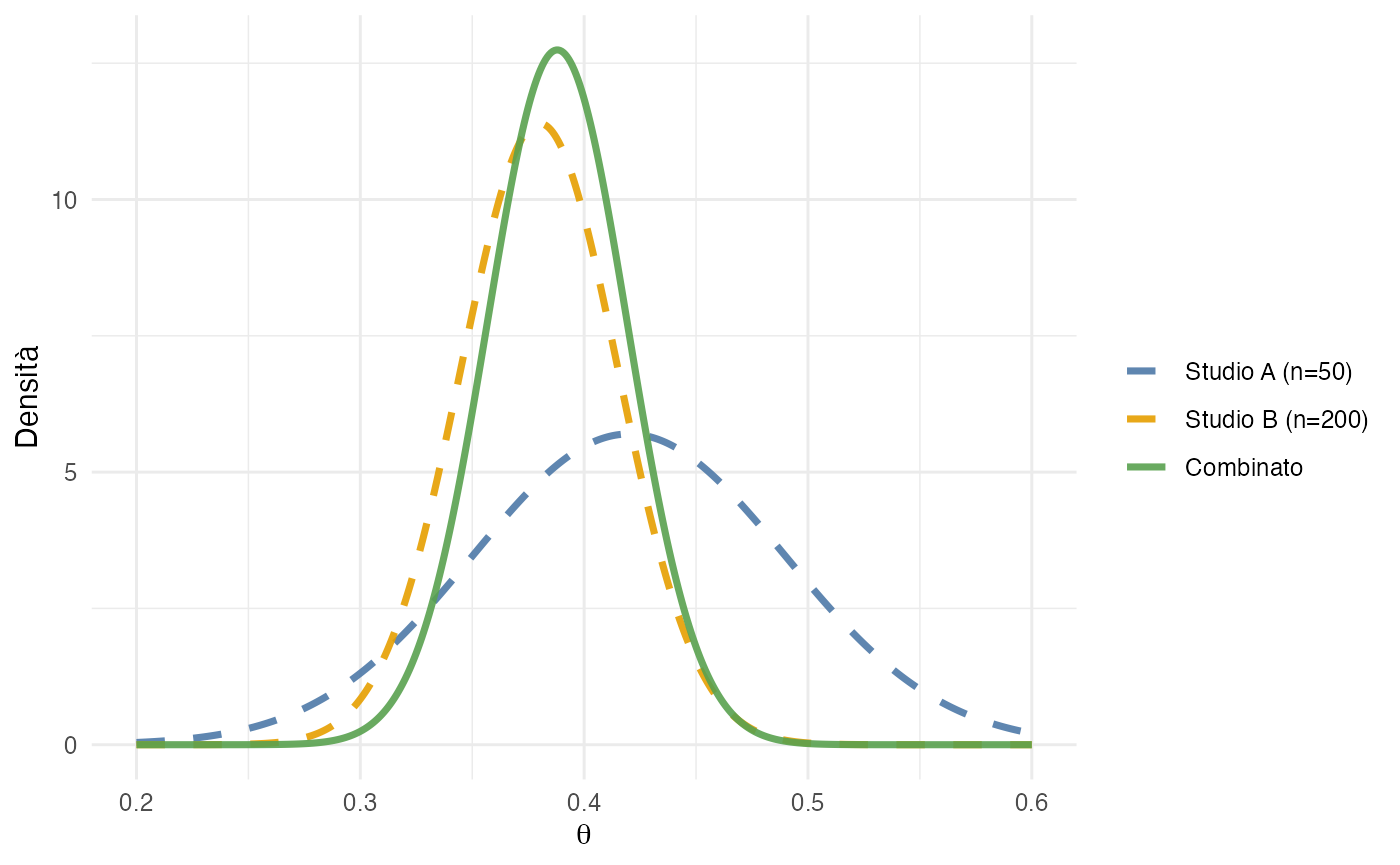
\includegraphics[width=0.85\linewidth,height=\textheight,keepaspectratio]{chapters/probability/15_properties_likelihood_files/figure-pdf/fig-meta-analysis-1.png}

}

\caption{\label{fig-meta-analysis}Combinazione di evidenze. Lo studio B
(n=200), avendo una precisione notevolmente maggiore, contribuisce di
più alla stima combinata (linea verde). L'intervallo di credibilità
risultante è più stretto di quello di ciascuno studio preso
singolarmente.}

\end{figure}%

\begin{tcolorbox}[enhanced jigsaw, arc=.35mm, breakable, colbacktitle=quarto-callout-note-color!10!white, opacityback=0, toprule=.15mm, rightrule=.15mm, colback=white, opacitybacktitle=0.6, leftrule=.75mm, coltitle=black, bottomtitle=1mm, left=2mm, toptitle=1mm, title=\textcolor{quarto-callout-note-color}{\faInfo}\hspace{0.5em}{Il peso dell'evidenza}, titlerule=0mm, bottomrule=.15mm, colframe=quarto-callout-note-color-frame]

La stima combinata (0.388) risulta più vicina al valore riportato dallo
studio B (0.38) rispetto a quello dello studio A (0.42). Ciò è dovuto al
fatto che lo studio B, grazie alla sua maggiore dimensione campionaria,
presenta una maggiore precisione e quindi riceve un peso maggiore nella
media ponderata. Il principio che emerge è intuitivo: nella sintesi
delle evidenze scientifiche, le stime basate su campioni più ampi e
quelle meno incerte esercitano un'influenza proporzionalmente maggiore
sul risultato finale, garantendo che la conclusione complessiva rifletta
in modo ottimale l'affidabilità delle fonti disponibili.

\end{tcolorbox}

\section{Limiti dell'inferenza: precisione
vs.~accuratezza}\label{limiti-dellinferenza-precisione-vs.-accuratezza}

\subsection{L'errore standard quantifica solo l'incertezza
campionaria}\label{lerrore-standard-quantifica-solo-lincertezza-campionaria}

È cruciale distinguere due dimensioni distinte dell'inferenza
statistica. Tutte le proprietà matematiche discusse in questo capitolo,
quali la convergenza della verosimiglianza, il restringimento della
distribuzione a posteriori e la riduzione dell'errore standard,
riguardano esclusivamente la \textbf{precisione} della stima, ovvero la
riduzione dell'incertezza dovuta alla variabilità campionaria.

Questi risultati non mitigano né possono correggere eventuali
\textbf{distorsioni sistematiche} (\emph{bias}) introdotte nelle fasi di
progettazione, misurazione o raccolta dei dati. Una stima può essere
estremamente precisa (con un intervallo di credibilità molto stretto),
ma può comunque essere profondamente inaccurata (lontana dal valore vero
del parametro) se è affetta da \emph{bias} non considerati.

\subsection{Fonti di distorsione
sistematica}\label{fonti-di-distorsione-sistematica}

Nella ricerca applicata, soprattutto in ambito psicologico e sociale,
sono frequenti distorsioni che alterano i risultati in modo prevedibile.
Anche un'analisi statistica formalmente corretta può condurre a
conclusioni fuorvianti se tali distorsioni non vengono prevenute o
controllate.

\textbf{Distorsione da selezione.} Si verifica quando il campione
studiato non rappresenta la popolazione a cui si desidera estendere le
inferenze. In questi casi, la generalizzabilità dei risultati è
compromessa. Tra le cause tipiche vi sono il basso tasso di
partecipazione, il reclutamento opportunistico (\emph{convenience
sampling}) o l'autoselezione, in cui partecipano preferenzialmente
individui con caratteristiche particolari (per esempio, maggiore
motivazione o familiarità con il tema).

\textbf{Distorsione da desiderabilità sociale.} Consiste nella tendenza
a fornire risposte ritenute più accettabili o approvate socialmente,
invece di riportare ciò che si pensa o si fa realmente. Questa
distorsione riguarda in particolare costrutti ``sensibili'' (come
pregiudizi, l'uso di sostanze e i problemi alimentari) e minaccia
soprattutto la validità di costrutto, poiché le risposte raccolte non
rappresentano più il fenomeno psicologico che si intende misurare.

\textbf{Errori di misurazione.} Si verificano quando gli strumenti
utilizzati non riescono a catturare correttamente il costrutto teorico o
producono misurazioni instabili. L'assenza di validità porta a misurare
qualcosa di diverso da ciò che si intende studiare, mentre l'assenza di
affidabilità introduce fluttuazioni casuali che aumentano il rumore e
nascondono il segnale reale. In entrambi i casi, le stime ottenute
risultano distorte o indebolite rispetto al fenomeno reale.

\subsection{Il paradosso della falsa
precisione}\label{il-paradosso-della-falsa-precisione}

\begin{figure}

\centering{

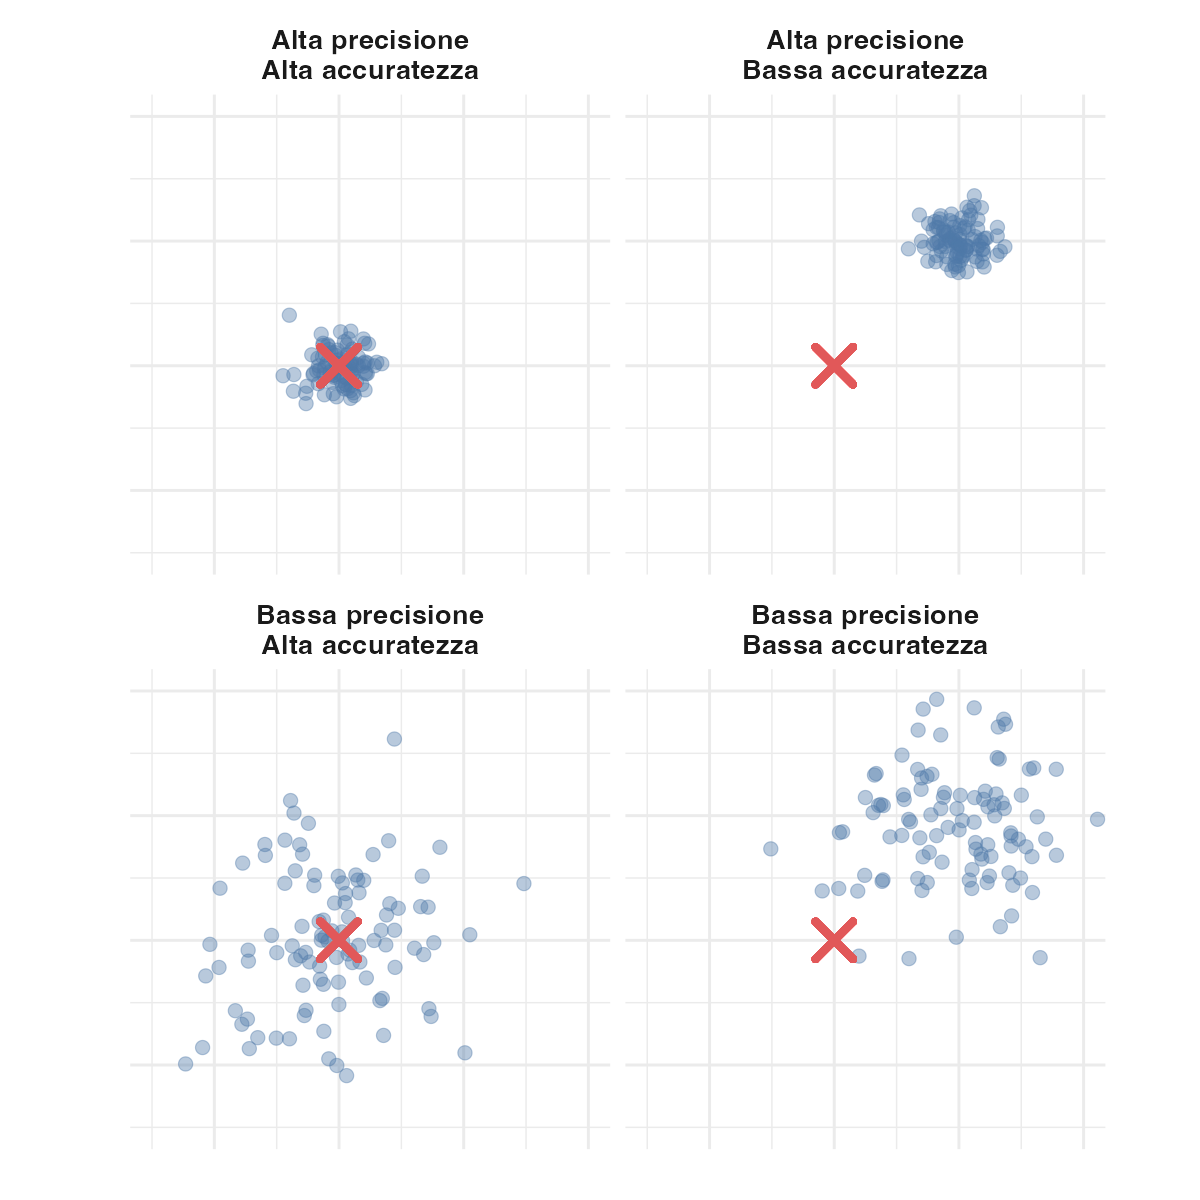
\includegraphics[width=0.85\linewidth,height=\textheight,keepaspectratio]{chapters/probability/15_properties_likelihood_files/figure-pdf/fig-precision-accuracy-1.png}

}

\caption{\label{fig-precision-accuracy}Precisione e accuratezza
nell'inferenza. La situazione più pericolosa è l'alta precisione con
bassa accuratezza (in alto a destra): stime molto sicure ma
sistematicamente sbagliate.}

\end{figure}%

\begin{tcolorbox}[enhanced jigsaw, arc=.35mm, breakable, colbacktitle=quarto-callout-warning-color!10!white, opacityback=0, toprule=.15mm, rightrule=.15mm, colback=white, opacitybacktitle=0.6, leftrule=.75mm, coltitle=black, bottomtitle=1mm, left=2mm, toptitle=1mm, title=\textcolor{quarto-callout-warning-color}{\faExclamationTriangle}\hspace{0.5em}{Il pericolo della falsa precisione}, titlerule=0mm, bottomrule=.15mm, colframe=quarto-callout-warning-color-frame]

La combinazione più insidiosa si verifica quando un'elevata precisione
si accompagna a una scarsa accuratezza (quadrante in alto a destra). In
questo scenario, il procedimento inferenziale produce intervalli di
credibilità molto stretti, che suggeriscono una grande certezza, attorno
a valori che sono invece sistematicamente distorti.

Un campione numericamente grande ma affetto da un bias sistematico può
essere \textbf{più fuorviante} di un campione piccolo ma non distorto:
genera stime apparentemente robuste che, però, consolidano una
conclusione errata, creando un'illusione di conoscenza scientificamente
fondata.

\end{tcolorbox}

\subsection{Strategie di mitigazione}\label{strategie-di-mitigazione}

La consapevolezza di questi limiti suggerisce alcune linee d'azione per
condurre una ricerca più solida.

\textbf{Progettazione metodologica rigorosa}: il controllo delle
distorsioni avviene principalmente nella fase di progettazione dello
studio, attraverso il campionamento probabilistico, la randomizzazione,
la definizione di protocolli standardizzati e la validazione degli
strumenti di misurazione.

\textbf{Analisi di sensibilità}: l'approccio bayesiano consente di
modellare esplicitamente le fonti di incertezza non campionaria e di
esplorare come le conclusioni cambino in base a diverse ipotesi
sull'entità dei possibili bias.

\textbf{Trasparenza epistemica}: è essenziale comunicare chiaramente che
gli intervalli di credibilità quantificano solo l'incertezza campionaria
e non l'affidabilità complessiva del disegno di ricerca. La valutazione
critica delle potenziali distorsioni rimane comunque un compito
fondamentale per il ricercatore.

\section*{Riflessioni conclusive}\label{riflessioni-conclusive-13}

\markright{Riflessioni conclusive}

Questo capitolo ha stabilito il collegamento fondamentale tra le
proprietà matematiche della distribuzione campionaria e il meccanismo
dell'aggiornamento bayesiano.

Le proprietà della media campionaria ---
\(\mathbb{E}[\bar{X}] = \theta\) e \(\text{Var}(\bar{X}) = \sigma^2/n\)
--- determinano la forma della funzione di verosimiglianza: centrata sul
valore osservato e sempre più concentrata all'aumentare dei dati. Queste
proprietà, a loro volta, determinano come la distribuzione a posteriori
risponde all'evidenza empirica.

Nel caso gaussiano l'aggiornamento assume una forma particolarmente
trasparente: la precisione a posteriori è la somma delle precisioni del
prior e dei dati, mentre la media a posteriori ne è la media ponderata.
Questo schema si generalizza, in modo approssimato, a una vasta classe
di modelli grazie al TLC, che giustifica l'approssimazione normale per
campioni sufficientemente ampi.

La LGN garantisce la \textbf{consistenza} dell'inferenza bayesiana: con
un numero sufficiente di osservazioni, la distribuzione a posteriori
converge al valore vero del parametro, indipendentemente dalla
distribuzione a priori adottata. Questo risultato conferisce robustezza
epistemica al procedimento: l'evidenza empirica, quando abbondante,
prevale sulle convinzioni iniziali.

Il TLC spiega l'ubiquità della forma normale nella distribuzione a
posteriori per campioni di grandi dimensioni, fornendo il fondamento
teorico per molte delle approssimazioni pratiche utilizzate
nell'inferenza.

È tuttavia cruciale riconoscere i \textbf{limiti} intrinseci di questi
risultati. Tutte le proprietà discusse si riferiscono esclusivamente
all'incertezza campionaria --- la variabilità introdotta dalla natura
casuale del campionamento. Esse non possono né correggere né mitigare
distorsioni sistematiche (bias) legate al disegno di ricerca o alla
misurazione. La precisione statistica, quindi, non deve mai essere
confusa con la validità scientifica.

Nei capitoli successivi del manuale principale, questi principi teorici
troveranno applicazione concreta nella costruzione, stima e
interpretazione di modelli bayesiani per la ricerca psicologica.

\begin{tcolorbox}[enhanced jigsaw, arc=.35mm, breakable, colbacktitle=quarto-callout-note-color!10!white, opacityback=0, toprule=.15mm, rightrule=.15mm, colback=white, opacitybacktitle=0.6, leftrule=.75mm, coltitle=black, bottomtitle=1mm, left=2mm, toptitle=1mm, title=\textcolor{quarto-callout-note-color}{\faInfo}\hspace{0.5em}{Informazioni sull'ambiente di sviluppo}, titlerule=0mm, bottomrule=.15mm, colframe=quarto-callout-note-color-frame]

\begin{Shaded}
\begin{Highlighting}[]
\FunctionTok{sessionInfo}\NormalTok{()}
\CommentTok{\#\textgreater{} R version 4.5.2 (2025{-}10{-}31)}
\CommentTok{\#\textgreater{} Platform: aarch64{-}apple{-}darwin20}
\CommentTok{\#\textgreater{} Running under: macOS Tahoe 26.1}
\CommentTok{\#\textgreater{} }
\CommentTok{\#\textgreater{} Matrix products: default}
\CommentTok{\#\textgreater{} BLAS:   /System/Library/Frameworks/Accelerate.framework/Versions/A/Frameworks/vecLib.framework/Versions/A/libBLAS.dylib }
\CommentTok{\#\textgreater{} LAPACK: /Library/Frameworks/R.framework/Versions/4.5{-}arm64/Resources/lib/libRlapack.dylib;  LAPACK version 3.12.1}
\CommentTok{\#\textgreater{} }
\CommentTok{\#\textgreater{} locale:}
\CommentTok{\#\textgreater{} [1] C.UTF{-}8/UTF{-}8/C.UTF{-}8/C/C.UTF{-}8/C.UTF{-}8}
\CommentTok{\#\textgreater{} }
\CommentTok{\#\textgreater{} time zone: Europe/Rome}
\CommentTok{\#\textgreater{} tzcode source: internal}
\CommentTok{\#\textgreater{} }
\CommentTok{\#\textgreater{} attached base packages:}
\CommentTok{\#\textgreater{} [1] stats     graphics  grDevices utils     datasets  methods   base     }
\CommentTok{\#\textgreater{} }
\CommentTok{\#\textgreater{} other attached packages:}
\CommentTok{\#\textgreater{}  [1] pillar\_1.11.1         tinytable\_0.15.1      patchwork\_1.3.2      }
\CommentTok{\#\textgreater{}  [4] ggdist\_3.3.3          tidybayes\_3.0.7       bayesplot\_1.14.0     }
\CommentTok{\#\textgreater{}  [7] ggplot2\_4.0.1         reliabilitydiag\_0.2.1 priorsense\_1.2.0     }
\CommentTok{\#\textgreater{} [10] posterior\_1.6.1       loo\_2.8.0             rstan\_2.32.7         }
\CommentTok{\#\textgreater{} [13] StanHeaders\_2.32.10   brms\_2.23.0           Rcpp\_1.1.0           }
\CommentTok{\#\textgreater{} [16] sessioninfo\_1.2.3     conflicted\_1.2.0      janitor\_2.2.1        }
\CommentTok{\#\textgreater{} [19] matrixStats\_1.5.0     modelr\_0.1.11         tibble\_3.3.0         }
\CommentTok{\#\textgreater{} [22] dplyr\_1.1.4           tidyr\_1.3.1           rio\_1.2.4            }
\CommentTok{\#\textgreater{} [25] here\_1.0.2           }
\CommentTok{\#\textgreater{} }
\CommentTok{\#\textgreater{} loaded via a namespace (and not attached):}
\CommentTok{\#\textgreater{}  [1] svUnit\_1.0.8          tidyselect\_1.2.1      farver\_2.1.2         }
\CommentTok{\#\textgreater{}  [4] S7\_0.2.1              fastmap\_1.2.0         TH.data\_1.1{-}5        }
\CommentTok{\#\textgreater{}  [7] tensorA\_0.36.2.1      digest\_0.6.39         timechange\_0.3.0     }
\CommentTok{\#\textgreater{} [10] estimability\_1.5.1    lifecycle\_1.0.4       survival\_3.8{-}3       }
\CommentTok{\#\textgreater{} [13] magrittr\_2.0.4        compiler\_4.5.2        rlang\_1.1.6          }
\CommentTok{\#\textgreater{} [16] tools\_4.5.2           yaml\_2.3.10           knitr\_1.50           }
\CommentTok{\#\textgreater{} [19] labeling\_0.4.3        bridgesampling\_1.2{-}1  curl\_7.0.0           }
\CommentTok{\#\textgreater{} [22] pkgbuild\_1.4.8        RColorBrewer\_1.1{-}3    abind\_1.4{-}8          }
\CommentTok{\#\textgreater{} [25] multcomp\_1.4{-}29       withr\_3.0.2           purrr\_1.2.0          }
\CommentTok{\#\textgreater{} [28] grid\_4.5.2            stats4\_4.5.2          colorspace\_2.1{-}2     }
\CommentTok{\#\textgreater{} [31] xtable\_1.8{-}4          inline\_0.3.21         emmeans\_2.0.0        }
\CommentTok{\#\textgreater{} [34] scales\_1.4.0          MASS\_7.3{-}65           cli\_3.6.5            }
\CommentTok{\#\textgreater{} [37] mvtnorm\_1.3{-}3         rmarkdown\_2.30        ragg\_1.5.0           }
\CommentTok{\#\textgreater{} [40] generics\_0.1.4        RcppParallel\_5.1.11{-}1 cachem\_1.1.0         }
\CommentTok{\#\textgreater{} [43] stringr\_1.6.0         splines\_4.5.2         parallel\_4.5.2       }
\CommentTok{\#\textgreater{} [46] vctrs\_0.6.5           V8\_8.0.1              Matrix\_1.7{-}4         }
\CommentTok{\#\textgreater{} [49] sandwich\_3.1{-}1        jsonlite\_2.0.0        arrayhelpers\_1.1{-}0   }
\CommentTok{\#\textgreater{} [52] systemfonts\_1.3.1     glue\_1.8.0            codetools\_0.2{-}20     }
\CommentTok{\#\textgreater{} [55] distributional\_0.5.0  lubridate\_1.9.4       stringi\_1.8.7        }
\CommentTok{\#\textgreater{} [58] gtable\_0.3.6          QuickJSR\_1.8.1        htmltools\_0.5.8.1    }
\CommentTok{\#\textgreater{} [61] Brobdingnag\_1.2{-}9     R6\_2.6.1              textshaping\_1.0.4    }
\CommentTok{\#\textgreater{} [64] rprojroot\_2.1.1       evaluate\_1.0.5        lattice\_0.22{-}7       }
\CommentTok{\#\textgreater{} [67] backports\_1.5.0       memoise\_2.0.1         broom\_1.0.10         }
\CommentTok{\#\textgreater{} [70] snakecase\_0.11.1      rstantools\_2.5.0      coda\_0.19{-}4.1        }
\CommentTok{\#\textgreater{} [73] gridExtra\_2.3         nlme\_3.1{-}168          checkmate\_2.3.3      }
\CommentTok{\#\textgreater{} [76] xfun\_0.54             zoo\_1.8{-}14            pkgconfig\_2.0.3}
\end{Highlighting}
\end{Shaded}

\end{tcolorbox}

\section*{Bibliografia}\label{bibliografia-11}

\markright{Bibliografia}

\cleardoublepage
\phantomsection
\addcontentsline{toc}{part}{Appendices}
\appendix

\chapter{Simbologia di base}\label{sec-apx-math-symbols}

Per una scrittura più sintetica possono essere utilizzati alcuni simboli
matematici.

\begin{itemize}
\tightlist
\item
  \(\log(x)\): il logaritmo naturale di \(x\).
\item
  L'operatore logico booleano \(\land\) significa ``e'' (congiunzione
  forte) mentre il connettivo di disgiunzione \(\lor\) significa ``o''
  (oppure) (congiunzione debole).
\item
  Il quantificatore esistenziale \(\exists\) vuol dire ``esiste almeno
  un'' e indica l'esistenza di almeno una istanza del concetto/oggetto
  indicato. Il quantificatore esistenziale di unicità \(\exists!\)
  (``esiste soltanto un'') indica l'esistenza di esattamente una istanza
  del concetto/oggetto indicato. Il quantificatore esistenziale
  \(\nexists\) nega l'esistenza del concetto/oggetto indicato.
\item
  Il quantificatore universale \(\forall\) vuol dire ``per ogni.''
\item
  \(\mathcal{A, S}\): insiemi.
\item
  \(x \in A\): \(x\) è un elemento dell'insieme \(A\).
\item
  L'implicazione logica ``\(\Rightarrow\)'' significa ``implica'' (se
  \ldots allora). \(P \Rightarrow Q\) vuol dire che \(P\) è condizione
  sufficiente per la verità di \(Q\) e che \(Q\) è condizione necessaria
  per la verità di \(P\).
\item
  L'equivalenza matematica ``\(\iff\)'' significa ``se e solo se'' e
  indica una condizione necessaria e sufficiente, o corrispondenza
  biunivoca.
\item
  Il simbolo \(\vert\) si legge ``tale che.''
\item
  Il simbolo \(\triangleq\) (o \(:=\)) si legge ``uguale per
  definizione.''
\item
  Il simbolo \(\Delta\) indica la differenza fra due valori della
  variabile scritta a destra del simbolo.
\item
  Il simbolo \(\propto\) si legge ``proporzionale a.''
\item
  Il simbolo \(\approx\) si legge ``circa.''
\item
  Il simbolo \(\in\) della teoria degli insiemi vuol dire ``appartiene''
  e indica l'appartenenza di un elemento ad un insieme. Il simbolo
  \(\notin\) vuol dire ``non appartiene.''
\item
  Il simbolo \(\subseteq\) si legge ``è un sottoinsieme di'' (può
  coincidere con l'insieme stesso). Il simbolo \(\subset\) si legge ``è
  un sottoinsieme proprio di.''
\item
  Il simbolo \(\#\) indica la cardinalità di un insieme.
\item
  Il simbolo \(\cap\) indica l'intersezione di due insiemi. Il simbolo
  \(\cup\) indica l'unione di due insiemi.
\item
  Il simbolo \(\emptyset\) indica l'insieme vuoto o evento impossibile.
\item
  In matematica, \(\mbox{argmax}\) identifica l'insieme dei punti per i
  quali una data funzione raggiunge il suo massimo. In altre parole,
  \(\mbox{argmax}_x f(x)\) è l'insieme dei valori di \(x\) per i quali
  \(f(x)\) raggiunge il valore più alto.
\item
  \(a, c, \alpha, \gamma\): scalari.
\item
  \(\boldsymbol{x}, \boldsymbol{y}\): vettori.
\item
  \(\boldsymbol{X}, \boldsymbol{Y}\): matrici.
\item
  \(X \sim p\): la variabile casuale \(X\) si distribuisce come \(p\).
\item
  \(p(\cdot)\): distribuzione di massa o di densità di probabilità.
\item
  \(p(y \mid \boldsymbol{x})\): la probabilità o densità di \(y\) dato
  \(\boldsymbol{x}\), ovvero
  \(p(y = \boldsymbol{Y} \mid x = \boldsymbol{X})\).
\item
  \(f(x)\): una funzione arbitraria di \(x\).
\item
  \(f(\boldsymbol{X}; \theta, \gamma)\): \(f\) è una funzione di
  \(\boldsymbol{X}\) con parametri \(\theta, \gamma\). Questa notazione
  indica che \(\boldsymbol{X}\) sono i dati che vengono passati ad un
  modello di parametri \(\theta, \gamma\).
\item
  \(\mathcal{N}(\mu, \sigma^2)\): distribuzione gaussiana di media
  \(\mu\) e varianza \(sigma^2\).
\item
  \(\mbox{Beta}(\alpha, \beta)\): distribuzione Beta di parametri
  \(\alpha\) e \(\beta\).
\item
  \(\mathcal{U}(a, b)\): distribuzione uniforme con limite inferiore
  \(a\) e limite superiore \(b\).
\item
  \(\mbox{Cauchy}(\alpha, \beta)\): distribuzione di Cauchy di parametri
  \(\alpha\) (posizione: media) e \(\beta\) (scala: radice quadrata
  della varianza).
\item
  \(\mathcal{B}(p)\): distribuzione di Bernoulli di parametro \(p\)
  (probabilità di successo).
\item
  \(\mbox{Bin}(n, p)\): distribuzione binomiale di parametri \(n\)
  (numero di prove) e \(p\) (probabilità di successo).
\item
  \(\mathbb{KL} (p \mid\mid q)\): la divergenza di Kullback-Leibler da
  \(p\) a \(q\).
\end{itemize}

\chapter{Numeri e intervalli}\label{sec-apx-numbers}

\section{Numeri binari}\label{numeri-binari}

I numeri binari rappresentano il sistema numerico più elementare
utilizzato in informatica, poiché sono composti unicamente da due
simboli: 0 e 1. Questa caratteristica li rende particolarmente adatti
alla rappresentazione di situazioni dicotomiche (vero/falso,
presente/assente) e consente ai computer di operare rapidamente ed
efficacemente sui dati.

Un esempio semplice d'impiego dei valori logici binari si ottiene quando
raccogliamo risposte a una domanda chiusa. Immaginiamo, ad esempio, di
porre la domanda ``Ti piacciono i mirtilli?'' a 10 studenti. Se le
risposte vengono memorizzate in R come valori logici (\texttt{TRUE} per
``Sì'' e \texttt{FALSE} per ``No''), potremmo avere:

\begin{Shaded}
\begin{Highlighting}[]
\NormalTok{opinion }\OtherTok{\textless{}{-}} \FunctionTok{c}\NormalTok{(}\ConstantTok{TRUE}\NormalTok{, }\ConstantTok{FALSE}\NormalTok{, }\ConstantTok{TRUE}\NormalTok{, }\ConstantTok{TRUE}\NormalTok{, }\ConstantTok{TRUE}\NormalTok{, }\ConstantTok{FALSE}\NormalTok{, }\ConstantTok{TRUE}\NormalTok{, }\ConstantTok{TRUE}\NormalTok{, }\ConstantTok{TRUE}\NormalTok{, }\ConstantTok{FALSE}\NormalTok{)}
\NormalTok{opinion}
\end{Highlighting}
\end{Shaded}

\begin{verbatim}
 [1]  TRUE FALSE  TRUE  TRUE  TRUE FALSE  TRUE  TRUE  TRUE FALSE
\end{verbatim}

In questo caso, \texttt{TRUE} e \texttt{FALSE} corrispondono a 1 e 0
rispettivamente quando utilizzati in operazioni numeriche. Lo stesso
avviene in Python, dove \texttt{True} è interpretato come 1 e
\texttt{False} come 0. Questa rappresentazione binaria permette di
ottenere facilmente statistiche sintetiche. Per esempio, per calcolare
la proporzione di risposte positive rispetto al totale, è sufficiente
sommare i valori (contando così il numero di \texttt{TRUE}) e dividere
per la lunghezza del vettore:

\begin{Shaded}
\begin{Highlighting}[]
\FunctionTok{sum}\NormalTok{(opinion) }\SpecialCharTok{/} \FunctionTok{length}\NormalTok{(opinion)}
\end{Highlighting}
\end{Shaded}

\begin{verbatim}
[1] 0.7
\end{verbatim}

Questo fornisce immediatamente la percentuale di studenti che hanno
risposto ``Sì'' alla domanda.

\begin{center}\rule{0.5\linewidth}{0.5pt}\end{center}

\section{Numeri interi}\label{numeri-interi}

I numeri interi sono caratterizzati dall'assenza di componenti decimali.
Essi includono sia i numeri naturali (1, 2, 3, \ldots), tradizionalmente
utilizzati per il conteggio, sia i loro opposti negativi. L'insieme dei
numeri naturali è indicato con \(\mathbb{N}\), mentre l'insieme dei
numeri interi (che include i numeri naturali, i loro negativi e lo zero)
si denota con \(\mathbb{Z}\):

\[
\mathbb{Z} = \{0, \pm 1, \pm 2, \pm 3, \dots\}
\]

\begin{center}\rule{0.5\linewidth}{0.5pt}\end{center}

\section{Numeri razionali}\label{numeri-razionali}

I numeri razionali sono quei numeri che possono essere espressi come il
rapporto tra due numeri interi, con il denominatore diverso da zero.
Essi formano l'insieme:

\[
\mathbb{Q} = \left\{\frac{m}{n} \mid m,n \in \mathbb{Z}, n \neq 0\right\}.
\]

Poiché ogni numero naturale è anche un intero, e ogni intero può essere
rappresentato come razionale (ad esempio \(5 = \frac{5}{1}\)), si ha una
catena d'inclusioni tra i diversi insiemi di numeri:

\[
\mathbb{N} \subseteq \mathbb{Z} \subseteq \mathbb{Q}.
\]

Se si desidera considerare solo i numeri razionali non negativi, si
utilizza la notazione:

\[
\mathbb{Q}^+ = \{q \in \mathbb{Q} \mid q \geq 0\}.
\]

\begin{center}\rule{0.5\linewidth}{0.5pt}\end{center}

\section{Numeri irrazionali}\label{numeri-irrazionali}

Non tutti i numeri possono essere espressi come rapporto di due interi.
I numeri che non hanno questa proprietà sono detti irrazionali. Essi non
possono essere scritti in forma frazionaria e la loro espansione
decimale è infinita e non periodica. Esempi tipici di numeri irrazionali
sono:

\begin{itemize}
\tightlist
\item
  \(\sqrt{2}\)
\item
  \(\sqrt{3}\)
\item
  \(\pi = 3.141592...\)
\end{itemize}

\begin{center}\rule{0.5\linewidth}{0.5pt}\end{center}

\section{Numeri reali}\label{numeri-reali}

I numeri razionali non coprono tutti i possibili punti sulla retta
reale. Per rappresentare ogni possibile misura, grandezza o punto su una
linea continua, si considerano i numeri reali, denotati con
\(\mathbb{R}\). L'insieme dei numeri reali comprende sia i razionali sia
gli irrazionali:

\[
\mathbb{N} \subseteq \mathbb{Z} \subseteq \mathbb{Q} \subseteq \mathbb{R}.
\]

In statistica, la precisione con cui si esprime una misura è spesso
legata al numero di cifre decimali utilizzate, sfruttando così appieno
la ``continuità'' offerta dai numeri reali.

\section{Intervalli Numerici}\label{intervalli-numerici}

\textbf{Definizione:} Un \textbf{intervallo numerico} è un sottoinsieme
connesso della retta reale. Intuitivamente, rappresenta tutti i numeri
reali compresi tra due estremi, che possono o meno essere inclusi
nell'intervallo stesso.

\textbf{Classificazione degli intervalli:} Gli intervalli vengono
classificati in base all'inclusione o meno degli estremi:

\begin{itemize}
\tightlist
\item
  \textbf{Intervallo chiuso:} Include entrambi gli estremi. Si indica
  con \([a, b]\) e rappresenta l'insieme dei numeri reali \(x\) tali che
  \(a \leq x \leq b\).
\item
  \textbf{Intervallo aperto:} Non include alcun estremo. Si indica con
  \((a, b)\) e rappresenta l'insieme dei numeri reali \(x\) tali che
  \(a < x < b\).
\item
  \textbf{Intervalli semiaperti:}

  \begin{itemize}
  \tightlist
  \item
    \textbf{Chiuso a sinistra e aperto a destra:} Include l'estremo
    sinistro ma non quello destro. Si indica con \([a, b)\) e
    rappresenta l'insieme dei numeri reali \(x\) tali che
    \(a \leq x < b\).
  \item
    \textbf{Aperto a sinistra e chiuso a destra:} Include l'estremo
    destro ma non quello sinistro. Si indica con \((a, b]\) e
    rappresenta l'insieme dei numeri reali \(x\) tali che
    \(a < x \leq b\).
  \end{itemize}
\end{itemize}

\textbf{Tabella riassuntiva:}

\begin{longtable}[]{@{}lll@{}}
\toprule\noalign{}
Intervallo & Notazione & Condizione \\
\midrule\noalign{}
\endhead
\bottomrule\noalign{}
\endlastfoot
Chiuso & \([a, b]\) & \(a \leq x \leq b\) \\
Aperto & \((a, b)\) & \(a < x < b\) \\
Chiuso a sinistra, aperto a destra & \([a, b)\) & \(a \leq x < b\) \\
Aperto a sinistra, chiuso a destra & \((a, b]\) & \(a < x \leq b\) \\
\end{longtable}

\textbf{Osservazioni:} * La scelta della notazione con parentesi quadre
o tonde indica rispettivamente l'inclusione o l'esclusione degli
estremi.

\chapter{Sommatorie}\label{sec-apx-sums}

Le somme sono uno strumento fondamentale in molti contesti matematici e
statistici, e per gestirle in modo efficace è essenziale disporre di una
notazione chiara e precisa. Consideriamo, ad esempio, la somma dei primi
\(n\) numeri interi, che può essere espressa come
\(1 + 2 + \dots + (n-1) + n\), dove i puntini di sospensione (\(\dots\))
indicano che la sequenza deve essere completata seguendo il pattern
definito dai termini precedenti e successivi. Tuttavia, una notazione
come \(1 + 7 + \dots + 73.6\) risulterebbe ambigua senza ulteriori
specifiche. In generale, ci troveremo di fronte a somme della forma

\[
x_1 + x_2 + \dots + x_n,
\]

dove \(x_n\) rappresenta un numero definito altrove. Sebbene questa
notazione con i puntini di sospensione sia utile in alcuni contesti, può
risultare poco chiara in altri. Per questo motivo, si preferisce
utilizzare la notazione di sommatoria:

\[
\sum_{i=1}^n x_i,
\]

che si legge ``sommatoria per \(i\) che va da \(1\) a \(n\) di
\(x_i\)''. Il simbolo \(\sum\) (la lettera sigma maiuscola dell'alfabeto
greco) rappresenta l'operazione di somma, \(x_i\) è il generico addendo,
mentre \(1\) e \(n\) sono gli \emph{estremi della sommatoria}, che
definiscono l'intervallo di variazione dell'indice \(i\). Solitamente,
l'estremo inferiore è \(1\), ma potrebbe essere qualsiasi altro numero
\(m < n\). Pertanto, possiamo scrivere:

\[
\sum_{i=1}^n x_i = x_1 + x_2 + \dots + x_n.
\]

Ad esempio, se i valori di \(x\) sono \(\{3, 11, 4, 7\}\), avremo:

\[
\sum_{i=1}^4 x_i = 3 + 11 + 4 + 7 = 25,
\]

dove \(x_1 = 3\), \(x_2 = 11\), e così via. La quantità \(x_i\) è detta
\emph{argomento} della sommatoria, mentre la variabile \(i\), che assume
valori interi successivi, è chiamata \emph{indice} della sommatoria.

La notazione di sommatoria può anche essere espressa nella forma:

\[
\sum_{P(i)} x_i,
\]

dove \(P(i)\) è una proposizione logica riguardante \(i\) che può essere
vera o falsa. Quando è evidente che si vogliono sommare tutte le \(n\)
osservazioni, la notazione può essere semplificata in \(\sum_{i} x_i\) o
addirittura \(\sum x_i\). L'indice \(i\) può essere sostituito da altre
lettere, come \(k, j, l, \dots\), a seconda del contesto.

\section{Manipolazione di somme}\label{manipolazione-di-somme}

Per semplificare i calcoli che coinvolgono le sommatorie, è utile
conoscere alcune proprietà fondamentali.

\subsection{Proprietà 1 (Somma di una
costante)}\label{proprietuxe0-1-somma-di-una-costante}

La sommatoria di \(n\) valori tutti uguali a una costante \(a\) è pari a
\(n\) volte la costante stessa:

\[
\sum_{i=1}^{n} a = \underbrace{a + a + \dots + a}_{n \text{ volte}} = n a.
\]

\subsection{Proprietà 2 (Proprietà
distributiva)}\label{proprietuxe0-2-proprietuxe0-distributiva}

Se l'argomento della sommatoria contiene una costante, è possibile
fattorizzarla. Ad esempio:

\[
\sum_{i=1}^{n} a x_i = a x_1 + a x_2 + \dots + a x_n = a (x_1 + x_2 + \dots + x_n) = a \sum_{i=1}^{n} x_i.
\]

\subsection{Proprietà 3 (Proprietà
associativa)}\label{proprietuxe0-3-proprietuxe0-associativa}

Se l'argomento della sommatoria è una somma, possiamo separare i
termini:

\[
\sum_{i=1}^{n} (a + x_i) = (a + x_1) + (a + x_2) + \dots + (a + x_n) = n a + \sum_{i=1}^{n} x_i.
\]

In generale, possiamo scrivere:

\[
\sum_{i=1}^{n} (x_i + y_i) = \sum_{i=1}^{n} x_i + \sum_{i=1}^{n} y_i.
\]

\subsection{Proprietà 4 (Operazioni
algebriche)}\label{proprietuxe0-4-operazioni-algebriche}

Se è necessario eseguire un'operazione algebrica (come l'elevamento a
potenza o il logaritmo) sull'argomento della sommatoria, questa
operazione deve essere eseguita prima della somma. Ad esempio:

\[
\sum_{i=1}^{n} x_i^2 = x_1^2 + x_2^2 + \dots + x_n^2 \neq \left( \sum_{i=1}^{n} x_i \right)^2.
\]

\subsection{Proprietà 5 (Prodotto di
termini)}\label{proprietuxe0-5-prodotto-di-termini}

Nel caso di un prodotto tra termini, il prodotto deve essere eseguito
prima della somma:

\[
\sum_{i=1}^{n} x_i y_i = x_1 y_1 + x_2 y_2 + \dots + x_n y_n.
\]

Infatti, \(a_1 b_1 + a_2 b_2 \neq (a_1 + a_2)(b_1 + b_2)\).

\section{Doppia sommatoria}\label{doppia-sommatoria}

In alcuni contesti, si incontrano espressioni con una doppia sommatoria
e un doppio indice:

\[
\sum_{i=1}^{n} \sum_{j=1}^{m} x_{ij}.
\]

Questa notazione implica che, per ogni valore dell'indice esterno \(i\)
(da \(1\) a \(n\)), si deve sviluppare la sommatoria interna per \(j\)
(da \(1\) a \(m\)). Ad esempio:

\[
\sum_{i=1}^{3} \sum_{j=4}^{6} x_{ij} = (x_{1,4} + x_{1,5} + x_{1,6}) + (x_{2,4} + x_{2,5} + x_{2,6}) + (x_{3,4} + x_{3,5} + x_{3,6}).
\]

Un caso particolare interessante è la doppia sommatoria del prodotto di
due variabili:

\[
\sum_{i=1}^{n} \sum_{j=1}^{n} x_i y_j.
\]

In questo caso, poiché \(x_i\) non dipende dall'indice \(j\), possiamo
estrarre \(x_i\) dalla sommatoria interna:

\[
\sum_{i=1}^{n} \left( x_i \sum_{j=1}^{n} y_j \right).
\]

Allo stesso modo, la sommatoria interna \(\sum_{j=1}^{n} y_j\) non
dipende da \(i\), quindi può essere estratta dalla sommatoria esterna:

\[
\sum_{i=1}^{n} \sum_{j=1}^{n} x_i y_j = \left( \sum_{i=1}^{n} x_i \right) \left( \sum_{j=1}^{n} y_j \right).
\]

\subsection{Esempio pratico}\label{esempio-pratico}

Consideriamo i vettori \(x = \{2, 3, 1\}\) e \(y = \{1, 4, 9\}\).
Calcoliamo la doppia sommatoria:

\[
\begin{aligned}
\sum_{i=1}^3 \sum_{j=1}^3 x_i y_j &= x_1 y_1 + x_1 y_2 + x_1 y_3 + x_2 y_1 + x_2 y_2 + x_2 y_3 + x_3 y_1 + x_3 y_2 + x_3 y_3 \\
&= 2 \times (1 + 4 + 9) + 3 \times (1 + 4 + 9) + 1 \times (1 + 4 + 9) \\
&= 2 \times 14 + 3 \times 14 + 1 \times 14 = 84.
\end{aligned}
\]

D'altra parte, il prodotto delle due sommatorie è:

\[
\left( \sum_{i=1}^3 x_i \right) \left( \sum_{j=1}^3 y_j \right) = (2 + 3 + 1) \times (1 + 4 + 9) = 6 \times 14 = 84.
\]

I due risultati coincidono, confermando la validità della proprietà.

Per ulteriori approfondimenti, si consiglia la consultazione del testo
\emph{Concrete Mathematics: A Foundation for Computer Science}
(\citeproc{ref-graham_concrete_1994}{Graham et al., 1994}).

Esercizi pratici sono disponibili sulla seguente
\href{https://math.libretexts.org/Courses/Cosumnes_River_College/Math_370\%3A_Precalculus/07\%3A_Sequences_and_the_Binomial_Theorem/7.02\%3A_Summation_Notation/7.2E\%3A_Exercises}{pagina
web}.

\section*{Bibliografia}\label{bibliografia-12}
\addcontentsline{toc}{section}{Bibliografia}

\markright{Bibliografia}

\chapter{Insiemi}\label{sec-apx-sets}

Un insieme (o collezione, classe, gruppo, \ldots) è stato definito da
Georg Cantor nel modo seguente:

\begin{quote}
un insieme è una collezione di oggetti, determinati e distinti, della
nostra percezione o del nostro pensiero, concepiti come un tutto unico;
tali oggetti si dicono elementi dell'insieme.
\end{quote}

Mentre non è rilevante la natura degli oggetti che costituiscono
l'insieme, ciò che importa è distinguere se un dato oggetto appartenga o
meno ad un insieme. Deve essere vera una delle due possibilità: il dato
oggetto è un elemento dell'insieme considerato oppure non è elemento
dell'insieme considerato. Due insiemi \(A\) e \(B\) si dicono uguali se
sono formati dagli stessi elementi, anche se disposti in ordine diverso:
\(A=B\). Due insiemi \(A\) e \(B\) si dicono diversi se non contengono
gli stessi elementi: \(A \neq B\). Ad esempio, i seguenti insiemi sono
uguali:

\[
\{1, 2, 3\} = \{3, 1, 2\} = \{1, 3, 2\}= \{1, 1, 1, 2, 3, 3, 3\}.
\]

Gli insiemi sono denotati da una lettera maiuscola, mentre le lettere
minuscole, di solito, designano gli elementi di un insieme. Per esempio,
un generico insieme \(A\) si indica con

\[
A = \{a_1, a_2, \dots, a_n\}, \quad \text{con } n > 0.
\]

La scrittura \(a \in A\) dice che \(a\) è un elemento di \(A\). Per dire
che \(b\) non è un elemento di \(A\) si scrive \(b \notin A.\)

Per quegli insiemi i cui elementi soddisfano una certa proprietà che li
caratterizza, tale proprietà può essere usata per descrivere più
sinteticamente l'insieme:

\[
A = \{x ~\vert~ \text{proprietà posseduta da } x\},
\]

che si legge come ``\(A\) è l'insieme degli elementi \(x\) per cui è
vera la proprietà indicata.'' Per esempio, per indicare l'insieme \(A\)
delle coppie di numeri reali \((x,y)\) che appartengono alla parabola
\(y = x^2 + 1\) si può scrivere:

\[
A = \{(x,y) ~\vert~ y = x^2 + 1\}.
\]

Dati due insiemi \(A\) e \(B\), diremo che \(A\) è un
\emph{sottoinsieme} di \(B\) se e solo se tutti gli elementi di \(A\)
sono anche elementi di \(B\):

\[
A \subseteq B \iff (\forall x \in A \Rightarrow x \in B).
\]

Se esiste almeno un elemento di \(B\) che non appartiene ad \(A\) allora
diremo che \(A\) è un \emph{sottoinsieme proprio} di \(B\):

\[
A \subset B \iff (A \subseteq B, \exists~ x \in B ~\vert~ x \notin A).
\]

Un altro insieme, detto \emph{insieme delle parti}, o insieme potenza,
che si associa all'insieme \(A\) è l'insieme di tutti i sottoinsiemi di
\(A\), inclusi l'insieme vuoto e \(A\) stesso. Per esempio, per
l'insieme \(A = \{a, b, c\}\), l'insieme delle parti è:

\[
\mathcal{P}(A) = \{
\emptyset, \{a\}, \{b\}, \{c\},
 \{a, b\}, \{a, c\}, \{c, b\},
 \{a, b, c\}
\}.
\]

\section{Diagrammi di Eulero-Venn}\label{diagrammi-di-eulero-venn}

I diagrammi di Venn sono uno strumento grafico molto utile per
rappresentare gli insiemi e per verificare le proprietà delle operazioni
tra di essi. Questi diagrammi prendono il nome dal matematico inglese
del 19° secolo John Venn, anche se rappresentazioni simili erano già
state utilizzate in precedenza da Leibniz e Eulero.

I diagrammi di Venn rappresentano gli insiemi come regioni del piano
delimitate da una curva chiusa. Nel caso di insiemi finiti, è possibile
evidenziare alcuni elementi di un insieme tramite punti, e in alcuni
casi possono essere evidenziati tutti gli elementi degli insiemi
considerati.

In sostanza, questi diagrammi sono un modo visuale per rappresentare le
proprietà degli insiemi e delle operazioni tra di essi. Sono uno
strumento molto utile per visualizzare la relazione tra gli insiemi e
per capire meglio come si combinano gli elementi all'interno di essi.

\section{Appartenenza ad un insieme}\label{appartenenza-ad-un-insieme}

Usiamo ora R

\begin{Shaded}
\begin{Highlighting}[]
\NormalTok{Set1 }\OtherTok{\textless{}{-}} \FunctionTok{c}\NormalTok{(}\DecValTok{1}\NormalTok{, }\DecValTok{2}\NormalTok{)}
\FunctionTok{print}\NormalTok{(Set1)}
\end{Highlighting}
\end{Shaded}

\begin{verbatim}
[1] 1 2
\end{verbatim}

\begin{Shaded}
\begin{Highlighting}[]
\FunctionTok{print}\NormalTok{(}\FunctionTok{class}\NormalTok{(Set1))}
\end{Highlighting}
\end{Shaded}

\begin{verbatim}
[1] "numeric"
\end{verbatim}

\begin{Shaded}
\begin{Highlighting}[]
\NormalTok{my\_list }\OtherTok{\textless{}{-}} \FunctionTok{c}\NormalTok{(}\DecValTok{1}\NormalTok{, }\DecValTok{2}\NormalTok{, }\DecValTok{3}\NormalTok{, }\DecValTok{4}\NormalTok{)}
\NormalTok{my\_set\_from\_list }\OtherTok{\textless{}{-}} \FunctionTok{unique}\NormalTok{(my\_list)}
\FunctionTok{print}\NormalTok{(my\_set\_from\_list)}
\end{Highlighting}
\end{Shaded}

\begin{verbatim}
[1] 1 2 3 4
\end{verbatim}

L'appartenenza ad un insieme si verifica con \texttt{\%in\%}.

\begin{Shaded}
\begin{Highlighting}[]
\NormalTok{my\_set }\OtherTok{\textless{}{-}} \FunctionTok{c}\NormalTok{(}\DecValTok{1}\NormalTok{, }\DecValTok{3}\NormalTok{, }\DecValTok{5}\NormalTok{)}
\FunctionTok{print}\NormalTok{(}\StringTok{"Ecco il mio insieme:"}\NormalTok{)}
\end{Highlighting}
\end{Shaded}

\begin{verbatim}
[1] "Ecco il mio insieme:"
\end{verbatim}

\begin{Shaded}
\begin{Highlighting}[]
\FunctionTok{print}\NormalTok{(my\_set)}
\end{Highlighting}
\end{Shaded}

\begin{verbatim}
[1] 1 3 5
\end{verbatim}

\begin{Shaded}
\begin{Highlighting}[]
\FunctionTok{print}\NormalTok{(}\StringTok{"1 appartiene all\textquotesingle{}insieme:"}\NormalTok{)}
\end{Highlighting}
\end{Shaded}

\begin{verbatim}
[1] "1 appartiene all'insieme:"
\end{verbatim}

\begin{Shaded}
\begin{Highlighting}[]
\FunctionTok{print}\NormalTok{(}\DecValTok{1} \SpecialCharTok{\%in\%}\NormalTok{ my\_set)}
\end{Highlighting}
\end{Shaded}

\begin{verbatim}
[1] TRUE
\end{verbatim}

\begin{Shaded}
\begin{Highlighting}[]
\FunctionTok{print}\NormalTok{(}\StringTok{"2 non appartiene all\textquotesingle{}insieme:"}\NormalTok{)}
\end{Highlighting}
\end{Shaded}

\begin{verbatim}
[1] "2 non appartiene all'insieme:"
\end{verbatim}

\begin{Shaded}
\begin{Highlighting}[]
\FunctionTok{print}\NormalTok{(}\DecValTok{2} \SpecialCharTok{\%in\%}\NormalTok{ my\_set)}
\end{Highlighting}
\end{Shaded}

\begin{verbatim}
[1] FALSE
\end{verbatim}

\begin{Shaded}
\begin{Highlighting}[]
\FunctionTok{print}\NormalTok{(}\StringTok{"4 NON appartiene all\textquotesingle{}insieme:"}\NormalTok{)}
\end{Highlighting}
\end{Shaded}

\begin{verbatim}
[1] "4 NON appartiene all'insieme:"
\end{verbatim}

\begin{Shaded}
\begin{Highlighting}[]
\FunctionTok{print}\NormalTok{(}\SpecialCharTok{!}\NormalTok{(}\DecValTok{4} \SpecialCharTok{\%in\%}\NormalTok{ my\_set))}
\end{Highlighting}
\end{Shaded}

\begin{verbatim}
[1] TRUE
\end{verbatim}

\section{Relazioni tra insiemi}\label{relazioni-tra-insiemi}

Esaminiamo le funzioni Python per descrivere le relazioni tra insiemi.
In particolare, dopo avere definito l'insieme universo e l'insieme
vuoto, considereremo la relazione di inclusione che conduce al concetto
di sottoinsieme. Analogamente si definisce il concetto di sovrainsieme.
Mostreremo anche come valutare se due insiemi sono disgiunti (si dicono
disgiunti gli insiemi con intersezione vuota).

\begin{Shaded}
\begin{Highlighting}[]
\NormalTok{Univ }\OtherTok{\textless{}{-}} \DecValTok{0}\SpecialCharTok{:}\DecValTok{10}
\NormalTok{Super }\OtherTok{\textless{}{-}}\NormalTok{ Univ[Univ }\SpecialCharTok{\%\%} \DecValTok{2} \SpecialCharTok{==} \DecValTok{0}\NormalTok{]}
\NormalTok{Disj }\OtherTok{\textless{}{-}}\NormalTok{ Univ[Univ }\SpecialCharTok{\%\%} \DecValTok{2} \SpecialCharTok{==} \DecValTok{1}\NormalTok{]}
\NormalTok{Sub }\OtherTok{\textless{}{-}} \FunctionTok{c}\NormalTok{(}\DecValTok{4}\NormalTok{, }\DecValTok{6}\NormalTok{)}
\NormalTok{Null }\OtherTok{\textless{}{-}}\NormalTok{ Univ[Univ }\SpecialCharTok{\textgreater{}} \DecValTok{10}\NormalTok{]}
\end{Highlighting}
\end{Shaded}

\begin{Shaded}
\begin{Highlighting}[]
\FunctionTok{print}\NormalTok{(}\StringTok{"Insieme Universo (tutti gli interi positivi fino a 10):"}\NormalTok{)}
\end{Highlighting}
\end{Shaded}

\begin{verbatim}
[1] "Insieme Universo (tutti gli interi positivi fino a 10):"
\end{verbatim}

\begin{Shaded}
\begin{Highlighting}[]
\FunctionTok{print}\NormalTok{(Univ)}
\end{Highlighting}
\end{Shaded}

\begin{verbatim}
 [1]  0  1  2  3  4  5  6  7  8  9 10
\end{verbatim}

\begin{Shaded}
\begin{Highlighting}[]
\FunctionTok{print}\NormalTok{(}\StringTok{"Tutti gli interi positivi pari fino a 10:"}\NormalTok{)}
\end{Highlighting}
\end{Shaded}

\begin{verbatim}
[1] "Tutti gli interi positivi pari fino a 10:"
\end{verbatim}

\begin{Shaded}
\begin{Highlighting}[]
\FunctionTok{print}\NormalTok{(Super)}
\end{Highlighting}
\end{Shaded}

\begin{verbatim}
[1]  0  2  4  6  8 10
\end{verbatim}

\begin{Shaded}
\begin{Highlighting}[]
\FunctionTok{print}\NormalTok{(}\StringTok{"Tutti gli interi positivi dispari fino a 10:"}\NormalTok{)}
\end{Highlighting}
\end{Shaded}

\begin{verbatim}
[1] "Tutti gli interi positivi dispari fino a 10:"
\end{verbatim}

\begin{Shaded}
\begin{Highlighting}[]
\FunctionTok{print}\NormalTok{(Disj)}
\end{Highlighting}
\end{Shaded}

\begin{verbatim}
[1] 1 3 5 7 9
\end{verbatim}

\begin{Shaded}
\begin{Highlighting}[]
\FunctionTok{print}\NormalTok{(}\StringTok{"Insieme di due elementi, 4 e 6:"}\NormalTok{)}
\end{Highlighting}
\end{Shaded}

\begin{verbatim}
[1] "Insieme di due elementi, 4 e 6:"
\end{verbatim}

\begin{Shaded}
\begin{Highlighting}[]
\FunctionTok{print}\NormalTok{(Sub)}
\end{Highlighting}
\end{Shaded}

\begin{verbatim}
[1] 4 6
\end{verbatim}

\begin{Shaded}
\begin{Highlighting}[]
\FunctionTok{print}\NormalTok{(}\StringTok{"Un insieme vuoto:"}\NormalTok{)}
\end{Highlighting}
\end{Shaded}

\begin{verbatim}
[1] "Un insieme vuoto:"
\end{verbatim}

\begin{Shaded}
\begin{Highlighting}[]
\FunctionTok{print}\NormalTok{(Null)}
\end{Highlighting}
\end{Shaded}

\begin{verbatim}
integer(0)
\end{verbatim}

\begin{Shaded}
\begin{Highlighting}[]
\FunctionTok{print}\NormalTok{(}\StringTok{\textquotesingle{}È "Super" un sovrainsieme di "Sub"?\textquotesingle{}}\NormalTok{)}
\end{Highlighting}
\end{Shaded}

\begin{verbatim}
[1] "È \"Super\" un sovrainsieme di \"Sub\"?"
\end{verbatim}

\begin{Shaded}
\begin{Highlighting}[]
\FunctionTok{print}\NormalTok{(}\FunctionTok{all}\NormalTok{(Sub }\SpecialCharTok{\%in\%}\NormalTok{ Super))}
\end{Highlighting}
\end{Shaded}

\begin{verbatim}
[1] TRUE
\end{verbatim}

\begin{Shaded}
\begin{Highlighting}[]
\FunctionTok{print}\NormalTok{(}\StringTok{\textquotesingle{}È "Super" un sottoinsieme di "Univ"?\textquotesingle{}}\NormalTok{)}
\end{Highlighting}
\end{Shaded}

\begin{verbatim}
[1] "È \"Super\" un sottoinsieme di \"Univ\"?"
\end{verbatim}

\begin{Shaded}
\begin{Highlighting}[]
\FunctionTok{print}\NormalTok{(}\FunctionTok{all}\NormalTok{(Super }\SpecialCharTok{\%in\%}\NormalTok{ Univ))}
\end{Highlighting}
\end{Shaded}

\begin{verbatim}
[1] TRUE
\end{verbatim}

\begin{Shaded}
\begin{Highlighting}[]
\FunctionTok{print}\NormalTok{(}\StringTok{\textquotesingle{}È "Sub" un sovrainsieme di "Super"?\textquotesingle{}}\NormalTok{)}
\end{Highlighting}
\end{Shaded}

\begin{verbatim}
[1] "È \"Sub\" un sovrainsieme di \"Super\"?"
\end{verbatim}

\begin{Shaded}
\begin{Highlighting}[]
\FunctionTok{print}\NormalTok{(}\FunctionTok{all}\NormalTok{(Super }\SpecialCharTok{\%in\%}\NormalTok{ Sub))}
\end{Highlighting}
\end{Shaded}

\begin{verbatim}
[1] FALSE
\end{verbatim}

\begin{Shaded}
\begin{Highlighting}[]
\FunctionTok{print}\NormalTok{(}\StringTok{\textquotesingle{}Sono "Super" e "Disj" insiemi disgiunti?\textquotesingle{}}\NormalTok{)}
\end{Highlighting}
\end{Shaded}

\begin{verbatim}
[1] "Sono \"Super\" e \"Disj\" insiemi disgiunti?"
\end{verbatim}

\begin{Shaded}
\begin{Highlighting}[]
\FunctionTok{print}\NormalTok{(}\FunctionTok{length}\NormalTok{(}\FunctionTok{intersect}\NormalTok{(Super, Disj)) }\SpecialCharTok{==} \DecValTok{0}\NormalTok{)}
\end{Highlighting}
\end{Shaded}

\begin{verbatim}
[1] TRUE
\end{verbatim}

\section{Operazioni tra insiemi}\label{operazioni-tra-insiemi}

Si definisce \emph{intersezione} di \(A\) e \(B\) l'insieme \(A \cap B\)
di tutti gli elementi \(x\) che appartengono ad \(A\) e
contemporaneamente a \(B\):

\[
A \cap B = \{x ~\vert~ x \in A \land x \in B\}.
\]

Si definisce \emph{unione} di \(A\) e \(B\) l'insieme \(A \cup B\) di
tutti gli elementi \(x\) che appartengono ad \(A\) o a \(B\), cioè

\[
A \cup B = \{x ~\vert~ x \in A \lor x \in B\}.
\]

\emph{Differenza}. Si indica con \(A \setminus B\) l'insieme degli
elementi di \(A\) che non appartengono a \(B\):

\[
A \setminus B = \{x ~\vert~ x \in A \land x \notin B\}.
\]

\emph{Insieme complementare}. Nel caso che sia \(B \subseteq A\),
l'insieme differenza \(A \setminus B\) è detto insieme complementare di
\(B\) in \(A\) e si indica con \(B^C\).

Dato un insieme \(S\), una \emph{partizione} di \(S\) è una collezione
di sottoinsiemi di \(S\), \(S_1, \dots, S_k\), tali che

\[
S = S_1 \cup S_2 \cup \dots S_k
\]

e

\[
S_i \cap S_j, \quad \text{con } i \neq j.
\]

La relazione tra unione, intersezione e insieme complementare è data
dalle leggi di DeMorgan:

\[
(A \cup B)^c = A^c \cap B^c,
\]

\[
(A \cap B)^c = A^c \cup B^c.
\]

In tutte le seguenti figure, \(S\) è la regione delimitata dal
rettangolo, \(L\) è la regione all'interno del cerchio di sinistra e
\(R\) è la regione all'interno del cerchio di destra. La regione
evidenziata mostra l'insieme indicato sotto ciascuna figura.

\begin{figure}[H]

{\centering \pandocbounded{\includegraphics[keepaspectratio]{chapters/appendix/../../figures/sets-venn-diagrams.png}}

}

\caption{Diagrammi di Venn}

\end{figure}%

I diagrammi di Eulero-Venn che illustrano le leggi di DeMorgan sono
forniti nella figura seguente.

\begin{figure}[H]

{\centering \pandocbounded{\includegraphics[keepaspectratio]{chapters/appendix/../../figures/demorgan.png}}

}

\caption{Leggi di DeMorgan}

\end{figure}%

Vediamo ora come si eseguono le operazioni tra insiemi con R.

\textbf{Intersezione.}

\begin{Shaded}
\begin{Highlighting}[]
\NormalTok{S1 }\OtherTok{\textless{}{-}} \FunctionTok{seq}\NormalTok{(}\DecValTok{1}\NormalTok{, }\DecValTok{10}\NormalTok{, }\AttributeTok{by =} \DecValTok{3}\NormalTok{)}
\NormalTok{S2 }\OtherTok{\textless{}{-}} \DecValTok{1}\SpecialCharTok{:}\DecValTok{6}
\NormalTok{S\_intersection }\OtherTok{\textless{}{-}} \FunctionTok{intersect}\NormalTok{(S1, S2)}
\FunctionTok{print}\NormalTok{(}\StringTok{"Intersezione di S1 e S2:"}\NormalTok{)}
\end{Highlighting}
\end{Shaded}

\begin{verbatim}
[1] "Intersezione di S1 e S2:"
\end{verbatim}

\begin{Shaded}
\begin{Highlighting}[]
\FunctionTok{print}\NormalTok{(S\_intersection)}
\end{Highlighting}
\end{Shaded}

\begin{verbatim}
[1] 1 4
\end{verbatim}

\textbf{Unione.} Si noti che il connettivo logico \texttt{\textbar{}}
corrisponde all'unione.

\begin{Shaded}
\begin{Highlighting}[]
\NormalTok{S\_union }\OtherTok{\textless{}{-}} \FunctionTok{union}\NormalTok{(S1, S2)}
\FunctionTok{print}\NormalTok{(}\StringTok{"Unione di S1 e S2:"}\NormalTok{)}
\end{Highlighting}
\end{Shaded}

\begin{verbatim}
[1] "Unione di S1 e S2:"
\end{verbatim}

\begin{Shaded}
\begin{Highlighting}[]
\FunctionTok{print}\NormalTok{(S\_union)}
\end{Highlighting}
\end{Shaded}

\begin{verbatim}
[1]  1  4  7 10  2  3  5  6
\end{verbatim}

\textbf{Insieme complementare.}

\begin{Shaded}
\begin{Highlighting}[]
\NormalTok{S }\OtherTok{\textless{}{-}} \FunctionTok{seq}\NormalTok{(}\DecValTok{0}\NormalTok{, }\DecValTok{20}\NormalTok{, }\AttributeTok{by =} \DecValTok{2}\NormalTok{)}
\NormalTok{S\_complement }\OtherTok{\textless{}{-}} \FunctionTok{setdiff}\NormalTok{(}\DecValTok{0}\SpecialCharTok{:}\DecValTok{20}\NormalTok{, S)}
\FunctionTok{print}\NormalTok{(}\StringTok{"S è l\textquotesingle{}insieme dei numeri interi pari tra 0 e 20:"}\NormalTok{)}
\end{Highlighting}
\end{Shaded}

\begin{verbatim}
[1] "S è l'insieme dei numeri interi pari tra 0 e 20:"
\end{verbatim}

\begin{Shaded}
\begin{Highlighting}[]
\FunctionTok{print}\NormalTok{(S)}
\end{Highlighting}
\end{Shaded}

\begin{verbatim}
 [1]  0  2  4  6  8 10 12 14 16 18 20
\end{verbatim}

\begin{Shaded}
\begin{Highlighting}[]
\FunctionTok{print}\NormalTok{(}\StringTok{"S\_complement è l\textquotesingle{}insieme dei numeri interi dispari tra 0 e 20:"}\NormalTok{)}
\end{Highlighting}
\end{Shaded}

\begin{verbatim}
[1] "S_complement è l'insieme dei numeri interi dispari tra 0 e 20:"
\end{verbatim}

\begin{Shaded}
\begin{Highlighting}[]
\FunctionTok{print}\NormalTok{(S\_complement)}
\end{Highlighting}
\end{Shaded}

\begin{verbatim}
 [1]  1  3  5  7  9 11 13 15 17 19
\end{verbatim}

\begin{Shaded}
\begin{Highlighting}[]
\FunctionTok{print}\NormalTok{(}\StringTok{"È l\textquotesingle{}unione di S e S\_complement uguale a tutti i numeri interi tra 0 e 20?"}\NormalTok{)}
\end{Highlighting}
\end{Shaded}

\begin{verbatim}
[1] "È l'unione di S e S_complement uguale a tutti i numeri interi tra 0 e 20?"
\end{verbatim}

\begin{Shaded}
\begin{Highlighting}[]
\FunctionTok{print}\NormalTok{(}\FunctionTok{setequal}\NormalTok{(}\FunctionTok{union}\NormalTok{(S, S\_complement), }\DecValTok{0}\SpecialCharTok{:}\DecValTok{20}\NormalTok{))}
\end{Highlighting}
\end{Shaded}

\begin{verbatim}
[1] TRUE
\end{verbatim}

\textbf{Differenza tra insiemi.}

\begin{Shaded}
\begin{Highlighting}[]
\NormalTok{S1 }\OtherTok{\textless{}{-}} \FunctionTok{seq}\NormalTok{(}\DecValTok{0}\NormalTok{, }\DecValTok{30}\NormalTok{, }\AttributeTok{by =} \DecValTok{3}\NormalTok{)}
\NormalTok{S2 }\OtherTok{\textless{}{-}} \FunctionTok{seq}\NormalTok{(}\DecValTok{0}\NormalTok{, }\DecValTok{30}\NormalTok{, }\AttributeTok{by =} \DecValTok{5}\NormalTok{)}
\FunctionTok{print}\NormalTok{(}\StringTok{"Differenza tra S2 e S1:"}\NormalTok{)}
\end{Highlighting}
\end{Shaded}

\begin{verbatim}
[1] "Differenza tra S2 e S1:"
\end{verbatim}

\begin{Shaded}
\begin{Highlighting}[]
\FunctionTok{print}\NormalTok{(}\FunctionTok{setdiff}\NormalTok{(S2, S1))}
\end{Highlighting}
\end{Shaded}

\begin{verbatim}
[1]  5 10 20 25
\end{verbatim}

\begin{Shaded}
\begin{Highlighting}[]
\FunctionTok{print}\NormalTok{(}\StringTok{"Differenza tra S1 e S2:"}\NormalTok{)}
\end{Highlighting}
\end{Shaded}

\begin{verbatim}
[1] "Differenza tra S1 e S2:"
\end{verbatim}

\begin{Shaded}
\begin{Highlighting}[]
\FunctionTok{print}\NormalTok{(}\FunctionTok{setdiff}\NormalTok{(S1, S2))}
\end{Highlighting}
\end{Shaded}

\begin{verbatim}
[1]  3  6  9 12 18 21 24 27
\end{verbatim}

\textbf{Differenza simmetrica.} La differenza simmetrica, indicata con
il simbolo Δ, è un'operazione insiemistica definita come unione tra la
differenza tra il primo e il secondo insieme e la differenza tra il
secondo e il primo insieme. In modo equivalente, la differenza
simmetrica equivale all'unione tra i due insiemi meno la loro
intersezione.

\begin{Shaded}
\begin{Highlighting}[]
\NormalTok{sym\_diff }\OtherTok{\textless{}{-}} \FunctionTok{union}\NormalTok{(}\FunctionTok{setdiff}\NormalTok{(S1, S2), }\FunctionTok{setdiff}\NormalTok{(S2, S1))}
\FunctionTok{print}\NormalTok{(}\StringTok{"Differenza simmetrica:"}\NormalTok{)}
\end{Highlighting}
\end{Shaded}

\begin{verbatim}
[1] "Differenza simmetrica:"
\end{verbatim}

\begin{Shaded}
\begin{Highlighting}[]
\FunctionTok{print}\NormalTok{(sym\_diff)}
\end{Highlighting}
\end{Shaded}

\begin{verbatim}
 [1]  3  6  9 12 18 21 24 27  5 10 20 25
\end{verbatim}

\section{Coppie ordinate e prodotto
cartesiano}\label{coppie-ordinate-e-prodotto-cartesiano}

Una coppia ordinata \((x,y)\) è l'insieme i cui elementi sono
\(x \in A\) e \(y \in B\) e nella quale \(x\) è la prima componente (o
prima coordinata) e \(y\) la seconda. L'insieme di tutte le coppie
ordinate costruite a partire dagli insiemi \(A\) e \(B\) viene detto
\textbf{prodotto cartesiano}:

\[
A \times B = \{(x, y) ~\vert~ x \in A \land y \in B\}.
\]

Ad esempio, sia \(A = \{1, 2, 3\}\) e \(B = \{a, b\}\). Allora,

\[
\{1, 2\} \times \{a, b, c\} = \{(1, a), (1, b), (1, c), (2, a), (2, b), (2, c)\}.
\]

Più in generale, un prodotto cartesiano di \(n\) insiemi può essere
rappresentato da un array di \(n\) dimensioni, dove ogni elemento è una
ennupla o tupla ordinata (ovvero, una collezione o un elenco ordinato di
\(n\) oggetti). Una n-pla ordinata si distingue da un insieme di \(n\)
elementi in quanto fra gli elementi di un insieme non è dato alcun
ordine. Inoltre gli elementi di una ennupla possono anche essere
ripetuti. Essendo la n-pla un elenco ordinato, in generale di ogni suo
elemento è possibile dire se sia il primo, il secondo, il terzo,
eccetera, fino all'n-esimo. Il prodotto cartesiano prende il nome da
René Descartes la cui formulazione della geometria analitica ha dato
origine al concetto.

\begin{Shaded}
\begin{Highlighting}[]
\NormalTok{A }\OtherTok{\textless{}{-}} \FunctionTok{c}\NormalTok{(}\StringTok{"a"}\NormalTok{, }\StringTok{"b"}\NormalTok{, }\StringTok{"c"}\NormalTok{)}
\NormalTok{S }\OtherTok{\textless{}{-}} \DecValTok{1}\SpecialCharTok{:}\DecValTok{3}
\NormalTok{cartesian\_product }\OtherTok{\textless{}{-}} \FunctionTok{expand.grid}\NormalTok{(A, S)}
\FunctionTok{print}\NormalTok{(}\StringTok{"Prodotto cartesiano di A e S:"}\NormalTok{)}
\end{Highlighting}
\end{Shaded}

\begin{verbatim}
[1] "Prodotto cartesiano di A e S:"
\end{verbatim}

\begin{Shaded}
\begin{Highlighting}[]
\FunctionTok{print}\NormalTok{(cartesian\_product)}
\end{Highlighting}
\end{Shaded}

\begin{verbatim}
  Var1 Var2
1    a    1
2    b    1
3    c    1
4    a    2
5    b    2
6    c    2
7    a    3
8    b    3
9    c    3
\end{verbatim}

Si definisce \emph{cardinalità} (o potenza) di un insieme finito il
numero degli elementi dell'insieme. Viene indicata con
\(\vert A\vert, \#(A)\) o \(\text{c}(A)\).

\begin{Shaded}
\begin{Highlighting}[]
\FunctionTok{print}\NormalTok{(}\StringTok{"La cardinalità dell\textquotesingle{}insieme prodotto cartesiano è:"}\NormalTok{)}
\end{Highlighting}
\end{Shaded}

\begin{verbatim}
[1] "La cardinalità dell'insieme prodotto cartesiano è:"
\end{verbatim}

\begin{Shaded}
\begin{Highlighting}[]
\FunctionTok{print}\NormalTok{(}\FunctionTok{nrow}\NormalTok{(cartesian\_product))}
\end{Highlighting}
\end{Shaded}

\begin{verbatim}
[1] 9
\end{verbatim}

\textbf{Potenza del prodotto cartesiano}

\begin{Shaded}
\begin{Highlighting}[]
\NormalTok{A }\OtherTok{\textless{}{-}} \FunctionTok{c}\NormalTok{(}\StringTok{"Head"}\NormalTok{, }\StringTok{"Tail"}\NormalTok{)}
\NormalTok{p2 }\OtherTok{\textless{}{-}} \FunctionTok{expand.grid}\NormalTok{(A, A)}
\FunctionTok{print}\NormalTok{(}\StringTok{"Il quadrato dell\textquotesingle{}insieme A è un insieme che contiene:"}\NormalTok{)}
\end{Highlighting}
\end{Shaded}

\begin{verbatim}
[1] "Il quadrato dell'insieme A è un insieme che contiene:"
\end{verbatim}

\begin{Shaded}
\begin{Highlighting}[]
\FunctionTok{print}\NormalTok{(}\FunctionTok{nrow}\NormalTok{(p2))}
\end{Highlighting}
\end{Shaded}

\begin{verbatim}
[1] 4
\end{verbatim}

\begin{Shaded}
\begin{Highlighting}[]
\FunctionTok{print}\NormalTok{(p2)}
\end{Highlighting}
\end{Shaded}

\begin{verbatim}
  Var1 Var2
1 Head Head
2 Tail Head
3 Head Tail
4 Tail Tail
\end{verbatim}

\begin{Shaded}
\begin{Highlighting}[]
\NormalTok{p3 }\OtherTok{\textless{}{-}} \FunctionTok{expand.grid}\NormalTok{(A, A, A)}
\FunctionTok{print}\NormalTok{(}\StringTok{"L\textquotesingle{}insieme A elevato alla terza potenza è costituito da:"}\NormalTok{)}
\end{Highlighting}
\end{Shaded}

\begin{verbatim}
[1] "L'insieme A elevato alla terza potenza è costituito da:"
\end{verbatim}

\begin{Shaded}
\begin{Highlighting}[]
\FunctionTok{print}\NormalTok{(}\FunctionTok{nrow}\NormalTok{(p3))}
\end{Highlighting}
\end{Shaded}

\begin{verbatim}
[1] 8
\end{verbatim}

\begin{Shaded}
\begin{Highlighting}[]
\FunctionTok{print}\NormalTok{(p3)}
\end{Highlighting}
\end{Shaded}

\begin{verbatim}
  Var1 Var2 Var3
1 Head Head Head
2 Tail Head Head
3 Head Tail Head
4 Tail Tail Head
5 Head Head Tail
6 Tail Head Tail
7 Head Tail Tail
8 Tail Tail Tail
\end{verbatim}

\chapter{Calcolo combinatorio}\label{sec-apx-combinatorics}

\begin{Shaded}
\begin{Highlighting}[]
\NormalTok{here}\SpecialCharTok{::}\FunctionTok{here}\NormalTok{(}\StringTok{"code"}\NormalTok{, }\StringTok{"\_common.R"}\NormalTok{) }\SpecialCharTok{|\textgreater{}}
    \FunctionTok{source}\NormalTok{()}

\ControlFlowTok{if}\NormalTok{ (}\SpecialCharTok{!}\FunctionTok{requireNamespace}\NormalTok{(}\StringTok{"pacman"}\NormalTok{)) }\FunctionTok{install.packages}\NormalTok{(}\StringTok{"pacman"}\NormalTok{)}
\NormalTok{pacman}\SpecialCharTok{::}\FunctionTok{p\_load}\NormalTok{(gtools, combinat)}
\end{Highlighting}
\end{Shaded}

Il \textbf{calcolo combinatorio} studia il numero di modi in cui è
possibile combinare, ordinare o disporre elementi appartenenti a uno o
più insiemi, seguendo regole ben definite. Molti problemi di probabilità
richiedono strumenti combinatori per determinare la probabilità di
eventi complessi. In questo capitolo, esploreremo i concetti
fondamentali del calcolo combinatorio, illustrandoli attraverso il
modello del \textbf{campionamento dall'urna}. Tratteremo i principi
della somma e del prodotto, fondamentali per affrontare problemi più
avanzati, come permutazioni, disposizioni e combinazioni.

\section{Principio della somma}\label{principio-della-somma-1}

Il \textbf{principio della somma} si applica quando un insieme di
elementi può essere suddiviso in \textbf{sottoinsiemi disgiunti} (ossia
senza sovrapposizioni). In questo caso, il numero totale di elementi è
dato dalla somma delle cardinalità dei sottoinsiemi:

\[
n_{\text{tot}} = n_1 + n_2 + \dots + n_k .
\]

\textbf{Esempio}

Un distributore contiene tre scomparti di caramelle, ciascuno con un
diverso tipo di dolci:

\begin{itemize}
\tightlist
\item
  \textbf{Scomparto A}: 10 caramelle alla menta,\\
\item
  \textbf{Scomparto B}: 8 caramelle alla frutta,\\
\item
  \textbf{Scomparto C}: 12 caramelle al cioccolato.
\end{itemize}

Quante caramelle ci sono in totale nel distributore?

Secondo il \textbf{principio della somma}, il numero totale di caramelle
è:

\[
n_{\text{tot}} = n_A + n_B + n_C = 10 + 8 + 12 = 30.
\]

Calcolo in R:

\begin{Shaded}
\begin{Highlighting}[]
\NormalTok{A }\OtherTok{\textless{}{-}} \DecValTok{10}
\NormalTok{B }\OtherTok{\textless{}{-}} \DecValTok{8}
\NormalTok{C }\OtherTok{\textless{}{-}} \DecValTok{12}

\NormalTok{totale\_caramelle }\OtherTok{\textless{}{-}}\NormalTok{ A }\SpecialCharTok{+}\NormalTok{ B }\SpecialCharTok{+}\NormalTok{ C}
\NormalTok{totale\_caramelle}
\CommentTok{\#\textgreater{} [1] 30}
\end{Highlighting}
\end{Shaded}

\textbf{Risultato}: Nel distributore ci sono \textbf{30 caramelle} in
totale.

\section{Principio del prodotto}\label{principio-del-prodotto-1}

Il \textbf{principio del prodotto} si applica quando un'operazione può
essere suddivisa in più \textbf{fasi indipendenti}, ciascuna con un
numero specifico di possibilità. In tal caso, il numero totale di
combinazioni è dato dal \textbf{prodotto} delle possibilità offerte da
ciascuna fase:

\[
n_{\text{tot}} = n_1 \cdot n_2 \cdot \dots \cdot n_k .
\]

\textbf{Esempio}

Supponiamo di avere quattro urne contenenti palline di diverso colore:

\begin{itemize}
\tightlist
\item
  \textbf{Urna A}: 5 palline,\\
\item
  \textbf{Urna B}: 6 palline,\\
\item
  \textbf{Urna C}: 3 palline,\\
\item
  \textbf{Urna D}: 2 palline.
\end{itemize}

Vogliamo formare insiemi di due palline, ciascuna estratta da urne
differenti.

Secondo il \textbf{principio del prodotto}, per ogni coppia di urne, il
numero di combinazioni è dato dal prodotto del numero di palline
contenute nelle due urne. Utilizziamo poi il \textbf{principio della
somma} per ottenere il totale complessivo:

\[
n_{\text{tot}} = AB + AC + AD + BC + BD + CD.
\]

Calcolo in R:

\begin{Shaded}
\begin{Highlighting}[]
\NormalTok{AB }\OtherTok{\textless{}{-}} \DecValTok{5} \SpecialCharTok{*} \DecValTok{6}
\NormalTok{AC }\OtherTok{\textless{}{-}} \DecValTok{5} \SpecialCharTok{*} \DecValTok{3}
\NormalTok{AD }\OtherTok{\textless{}{-}} \DecValTok{5} \SpecialCharTok{*} \DecValTok{2}
\NormalTok{BC }\OtherTok{\textless{}{-}} \DecValTok{6} \SpecialCharTok{*} \DecValTok{3}
\NormalTok{BD }\OtherTok{\textless{}{-}} \DecValTok{6} \SpecialCharTok{*} \DecValTok{2}
\NormalTok{CD }\OtherTok{\textless{}{-}} \DecValTok{3} \SpecialCharTok{*} \DecValTok{2}

\NormalTok{totale\_insiemi }\OtherTok{\textless{}{-}}\NormalTok{ AB }\SpecialCharTok{+}\NormalTok{ AC }\SpecialCharTok{+}\NormalTok{ AD }\SpecialCharTok{+}\NormalTok{ BC }\SpecialCharTok{+}\NormalTok{ BD }\SpecialCharTok{+}\NormalTok{ CD}
\NormalTok{totale\_insiemi}
\CommentTok{\#\textgreater{} [1] 91}
\end{Highlighting}
\end{Shaded}

\textbf{Risultato}: È possibile formare \textbf{91 insiemi} di due
palline, ciascuna estratta da urne differenti.

\section{Il modello dell'urna e i metodi di
campionamento}\label{il-modello-dellurna-e-i-metodi-di-campionamento}

Molti problemi di calcolo combinatorio possono essere interpretati come
\textbf{estrazioni di palline da un'urna}. Esistono quattro modi
fondamentali di effettuare un campionamento, a seconda che:

\begin{enumerate}
\def\labelenumi{\arabic{enumi}.}
\tightlist
\item
  le estrazioni siano con o senza ripetizione,
\item
  l'ordine degli elementi conti o meno.
\end{enumerate}

Queste quattro combinazioni danno origine a quattro principali metodi di
campionamento:

\begin{enumerate}
\def\labelenumi{\arabic{enumi}.}
\tightlist
\item
  \textbf{Con ripetizione e con ordine}: Dopo ogni estrazione, la
  pallina viene rimessa nell'urna. (Es. formazione di codici numerici
  con ripetizioni)
\item
  \textbf{Senza ripetizione e con ordine}: Ogni estrazione rimuove
  definitivamente la pallina dall'urna. (Es. assegnare premi in una
  gara)
\item
  \textbf{Con ripetizione e senza ordine}: Si considerano i gruppi di
  elementi senza preoccuparsi dell'ordine. (Es. selezionare un certo
  numero di ingredienti da una dispensa)
\item
  \textbf{Senza ripetizione e senza ordine}: Si scelgono elementi
  distinti senza considerare l'ordine. (Es. formare squadre da un gruppo
  di persone)
\end{enumerate}

\begin{example}[]\protect\hypertarget{exm-}{}\label{exm-}

~

\begin{Shaded}
\begin{Highlighting}[]
\NormalTok{urna }\OtherTok{\textless{}{-}} \FunctionTok{c}\NormalTok{(}\StringTok{"a"}\NormalTok{, }\StringTok{"b"}\NormalTok{, }\StringTok{"c"}\NormalTok{)}

\CommentTok{\# Con ripetizione e ordine}
\NormalTok{campionamento1 }\OtherTok{\textless{}{-}} \FunctionTok{expand.grid}\NormalTok{(urna, urna) }\SpecialCharTok{|\textgreater{}}
    \FunctionTok{rename}\NormalTok{(}\AttributeTok{Elemento1 =}\NormalTok{ Var1, }\AttributeTok{Elemento2 =}\NormalTok{ Var2)}

\CommentTok{\# Senza ripetizione e con ordine}
\NormalTok{campionamento2 }\OtherTok{\textless{}{-}} \FunctionTok{permutations}\NormalTok{(}\AttributeTok{n =} \FunctionTok{length}\NormalTok{(urna), }\AttributeTok{r =} \DecValTok{2}\NormalTok{, }\AttributeTok{v =}\NormalTok{ urna) }\SpecialCharTok{|\textgreater{}}
    \FunctionTok{as.data.frame}\NormalTok{() }\SpecialCharTok{|\textgreater{}}
    \FunctionTok{rename}\NormalTok{(}\AttributeTok{Elemento1 =}\NormalTok{ V1, }\AttributeTok{Elemento2 =}\NormalTok{ V2)}

\CommentTok{\# Con ripetizione e senza ordine}
\NormalTok{campionamento3 }\OtherTok{\textless{}{-}} \FunctionTok{combinations}\NormalTok{(}
    \AttributeTok{n =} \FunctionTok{length}\NormalTok{(urna), }\AttributeTok{r =} \DecValTok{2}\NormalTok{, }\AttributeTok{v =}\NormalTok{ urna, }\AttributeTok{repeats.allowed =} \ConstantTok{TRUE}
\NormalTok{) }\SpecialCharTok{|\textgreater{}}
    \FunctionTok{as.data.frame}\NormalTok{() }\SpecialCharTok{|\textgreater{}}
    \FunctionTok{rename}\NormalTok{(}\AttributeTok{Elemento1 =}\NormalTok{ V1, }\AttributeTok{Elemento2 =}\NormalTok{ V2)}

\CommentTok{\# Senza ripetizione e senza ordine}
\NormalTok{campionamento4 }\OtherTok{\textless{}{-}} \FunctionTok{combinations}\NormalTok{(}\AttributeTok{n =} \FunctionTok{length}\NormalTok{(urna), }\AttributeTok{r =} \DecValTok{2}\NormalTok{, }\AttributeTok{v =}\NormalTok{ urna) }\SpecialCharTok{|\textgreater{}}
    \FunctionTok{as.data.frame}\NormalTok{() }\SpecialCharTok{|\textgreater{}}
    \FunctionTok{rename}\NormalTok{(}\AttributeTok{Elemento1 =}\NormalTok{ V1, }\AttributeTok{Elemento2 =}\NormalTok{ V2)}

\CommentTok{\# Risultati}
\FunctionTok{list}\NormalTok{(}
    \StringTok{\textasciigrave{}}\AttributeTok{Con ripetizione e ordine}\StringTok{\textasciigrave{}} \OtherTok{=}\NormalTok{ campionamento1,}
    \StringTok{\textasciigrave{}}\AttributeTok{Senza ripetizione e con ordine}\StringTok{\textasciigrave{}} \OtherTok{=}\NormalTok{ campionamento2,}
    \StringTok{\textasciigrave{}}\AttributeTok{Con ripetizione e senza ordine}\StringTok{\textasciigrave{}} \OtherTok{=}\NormalTok{ campionamento3,}
    \StringTok{\textasciigrave{}}\AttributeTok{Senza ripetizione e senza ordine}\StringTok{\textasciigrave{}} \OtherTok{=}\NormalTok{ campionamento4}
\NormalTok{)}
\CommentTok{\#\textgreater{} $\textasciigrave{}Con ripetizione e ordine\textasciigrave{}}
\CommentTok{\#\textgreater{}   Elemento1 Elemento2}
\CommentTok{\#\textgreater{} 1         a         a}
\CommentTok{\#\textgreater{} 2         b         a}
\CommentTok{\#\textgreater{} 3         c         a}
\CommentTok{\#\textgreater{} 4         a         b}
\CommentTok{\#\textgreater{} 5         b         b}
\CommentTok{\#\textgreater{} 6         c         b}
\CommentTok{\#\textgreater{} 7         a         c}
\CommentTok{\#\textgreater{} 8         b         c}
\CommentTok{\#\textgreater{} 9         c         c}
\CommentTok{\#\textgreater{} }
\CommentTok{\#\textgreater{} $\textasciigrave{}Senza ripetizione e con ordine\textasciigrave{}}
\CommentTok{\#\textgreater{}   Elemento1 Elemento2}
\CommentTok{\#\textgreater{} 1         a         b}
\CommentTok{\#\textgreater{} 2         a         c}
\CommentTok{\#\textgreater{} 3         b         a}
\CommentTok{\#\textgreater{} 4         b         c}
\CommentTok{\#\textgreater{} 5         c         a}
\CommentTok{\#\textgreater{} 6         c         b}
\CommentTok{\#\textgreater{} }
\CommentTok{\#\textgreater{} $\textasciigrave{}Con ripetizione e senza ordine\textasciigrave{}}
\CommentTok{\#\textgreater{}   Elemento1 Elemento2}
\CommentTok{\#\textgreater{} 1         a         a}
\CommentTok{\#\textgreater{} 2         a         b}
\CommentTok{\#\textgreater{} 3         a         c}
\CommentTok{\#\textgreater{} 4         b         b}
\CommentTok{\#\textgreater{} 5         b         c}
\CommentTok{\#\textgreater{} 6         c         c}
\CommentTok{\#\textgreater{} }
\CommentTok{\#\textgreater{} $\textasciigrave{}Senza ripetizione e senza ordine\textasciigrave{}}
\CommentTok{\#\textgreater{}   Elemento1 Elemento2}
\CommentTok{\#\textgreater{} 1         a         b}
\CommentTok{\#\textgreater{} 2         a         c}
\CommentTok{\#\textgreater{} 3         b         c}
\end{Highlighting}
\end{Shaded}

\end{example}

\section{Permutazioni: Disporre tutti gli elementi con
ordine}\label{permutazioni-disporre-tutti-gli-elementi-con-ordine}

Le \textbf{permutazioni} rappresentano tutti i modi in cui è possibile
ordinare \(n\) elementi distinti. Il numero di permutazioni è dato da:

\[
P_n = n!
\]

dove \(n!\) (n fattoriale) è il prodotto di tutti i numeri da 1 a \(n\):

\[
n! = n \cdot (n-1) \cdot (n-2) \cdot \dots \cdot 1.
\]

\subsection{Intuizione della formula}\label{intuizione-della-formula}

Immaginiamo di avere \textbf{\(n\) elementi distinti} e di doverli
disporre in una sequenza. Il primo elemento può essere scelto in
\textbf{\(n\) modi}. Una volta scelto il primo, rimangono
\textbf{\(n-1\) possibilità} per il secondo, poi \textbf{\(n-2\)} per il
terzo e così via, fino all'ultimo elemento, che avrà \textbf{1 sola
possibilità}. Applicando il \textbf{principio del prodotto}, otteniamo:

\[
P_n = n \times (n-1) \times (n-2) \times \dots \times 1 = n!
\]

\subsection{Metodo di campionamento
corrispondente}\label{metodo-di-campionamento-corrispondente}

\begin{itemize}
\tightlist
\item
  \textbf{Campionamento senza ripetizione e con ordine}: si estrae una
  pallina, la si esclude dall'urna e si continua fino a esaurire gli
  elementi.\\
\item
  \textbf{Esempio pratico}: Ordinare i partecipanti di una gara su un
  podio (primo, secondo e terzo classificato).
\end{itemize}

\subsection{Esempio in R: Permutazioni di tre
elementi}\label{esempio-in-r-permutazioni-di-tre-elementi}

Se abbiamo tre lettere \{a, b, c\}, le possibili permutazioni sono:

\[
P_3 = 3! = 3 \times 2 \times 1 = 6.
\]

\begin{Shaded}
\begin{Highlighting}[]
\NormalTok{A }\OtherTok{\textless{}{-}} \FunctionTok{c}\NormalTok{(}\StringTok{"a"}\NormalTok{, }\StringTok{"b"}\NormalTok{, }\StringTok{"c"}\NormalTok{)}
\NormalTok{perm }\OtherTok{\textless{}{-}} \FunctionTok{permutations}\NormalTok{(}\AttributeTok{n =} \FunctionTok{length}\NormalTok{(A), }\AttributeTok{r =} \FunctionTok{length}\NormalTok{(A), }\AttributeTok{v =}\NormalTok{ A)}
\FunctionTok{print}\NormalTok{(perm)}
\CommentTok{\#\textgreater{}      [,1] [,2] [,3]}
\CommentTok{\#\textgreater{} [1,] "a"  "b"  "c" }
\CommentTok{\#\textgreater{} [2,] "a"  "c"  "b" }
\CommentTok{\#\textgreater{} [3,] "b"  "a"  "c" }
\CommentTok{\#\textgreater{} [4,] "b"  "c"  "a" }
\CommentTok{\#\textgreater{} [5,] "c"  "a"  "b" }
\CommentTok{\#\textgreater{} [6,] "c"  "b"  "a"}
\FunctionTok{nrow}\NormalTok{(perm)  }\CommentTok{\# Verifica del numero di permutazioni}
\CommentTok{\#\textgreater{} [1] 6}
\end{Highlighting}
\end{Shaded}

\textbf{Risultato}:

\[
\{a, b, c\}, \{a, c, b\}, \{b, a, c\}, \{b, c, a\}, \{c, a, b\}, \{c, b, a\}.
\]

\section{Disposizioni: Selezionare alcuni elementi con
ordine}\label{disposizioni-selezionare-alcuni-elementi-con-ordine}

Le \textbf{disposizioni} si usano quando si scelgono \(k\) elementi da
un insieme di \(n\), rispettando l'ordine. Il numero totale di
disposizioni è:

\[
D_{n,k} = \frac{n!}{(n-k)!} .
\]

\subsection{Intuizione della formula}\label{intuizione-della-formula-1}

Supponiamo di avere \textbf{\(n\) elementi} e di voler scegliere solo
\textbf{\(k\) elementi}, mantenendo l'ordine.

\begin{itemize}
\tightlist
\item
  il primo elemento può essere scelto in \textbf{\(n\) modi};
\item
  il secondo elemento può essere scelto tra gli \textbf{\(n-1\) elementi
  rimanenti};\\
\item
  il terzo tra gli \textbf{\(n-2\)} rimanenti.
\end{itemize}

Si prosegue fino a quando si hanno scelto \textbf{\(k\) elementi},
fermandosi prima di esaurire tutti gli elementi.

\[
D_{n,k} = n \times (n-1) \times (n-2) \times \dots \times (n-k+1) .
\]

Questa espressione corrisponde alla divisione del fattoriale di \(n\)
per il fattoriale degli elementi che non vengono selezionati:

\[
D_{n,k} = \frac{n!}{(n-k)!} .
\]

\subsection{Metodo di campionamento
corrispondente}\label{metodo-di-campionamento-corrispondente-1}

\begin{itemize}
\tightlist
\item
  \textbf{Campionamento senza ripetizione e con ordine}: si estrae una
  pallina, la si esclude dall'urna e si continua fino a raggiungere il
  numero desiderato di elementi, fermandosi prima di esaurire tutti gli
  elementi.\\
\item
  \textbf{Esempio pratico}: Estrarre casualmente 2 studenti da una
  classe di 10 e assegnare loro i ruoli di rappresentante e
  vice-rappresentante (l'ordine conta).
\end{itemize}

\subsection{Esempio in R: Disposizioni di 2 elementi da \{a, b,
c\}}\label{esempio-in-r-disposizioni-di-2-elementi-da-a-b-c}

Se scegliamo 2 lettere su 3, il numero di disposizioni è:

\[
D_{3,2} = \frac{3!}{(3-2)!} = \frac{3 \times 2 \times 1}{1} = 6.
\]

\begin{Shaded}
\begin{Highlighting}[]
\NormalTok{disp }\OtherTok{\textless{}{-}} \FunctionTok{permutations}\NormalTok{(}\AttributeTok{n =} \FunctionTok{length}\NormalTok{(A), }\AttributeTok{r =} \DecValTok{2}\NormalTok{, }\AttributeTok{v =}\NormalTok{ A)}
\FunctionTok{print}\NormalTok{(disp)}
\CommentTok{\#\textgreater{}      [,1] [,2]}
\CommentTok{\#\textgreater{} [1,] "a"  "b" }
\CommentTok{\#\textgreater{} [2,] "a"  "c" }
\CommentTok{\#\textgreater{} [3,] "b"  "a" }
\CommentTok{\#\textgreater{} [4,] "b"  "c" }
\CommentTok{\#\textgreater{} [5,] "c"  "a" }
\CommentTok{\#\textgreater{} [6,] "c"  "b"}
\FunctionTok{nrow}\NormalTok{(disp)  }\CommentTok{\# Verifica del numero di disposizioni}
\CommentTok{\#\textgreater{} [1] 6}
\end{Highlighting}
\end{Shaded}

\textbf{Risultato}:

\[
\{a, b\}, \{a, c\}, \{b, a\}, \{b, c\}, \{c, a\}, \{c, b\}.
\]

Le disposizioni \textbf{considerano l'ordine}, quindi \(\{a, b\}\) è
diverso da \(\{b, a\}\).

\section{Combinazioni: Selezionare alcuni elementi senza
ordine}\label{combinazioni-selezionare-alcuni-elementi-senza-ordine}

Le \textbf{combinazioni} rappresentano il numero di modi per scegliere
\(k\) elementi da \(n\) \textbf{senza considerare l'ordine}. Il numero
di combinazioni è dato da:

\[
C_{n,k} = \binom{n}{k} = \frac{n!}{k!(n-k)!} .
\]

\subsection{Intuizione della formula}\label{intuizione-della-formula-2}

Supponiamo di avere \textbf{\(n\) elementi} e di voler selezionare
\textbf{\(k\) elementi} \textbf{senza considerare l'ordine}.\\
Come nel caso delle disposizioni, il primo elemento può essere scelto in
\textbf{\(n\) modi}, il secondo in \textbf{\(n-1\)}, e così via fino a
selezionare \textbf{\(k\) elementi}.

\[
D_{n,k} = n \times (n-1) \times \dots \times (n-k+1) .
\]

Tuttavia, in questo caso, l'ordine \textbf{non} conta, quindi ogni
selezione viene \textbf{duplicata} per il numero di modi in cui i \(k\)
elementi possono essere ordinati, ossia \textbf{\(k!\) permutazioni
interne}. Per correggere questa duplicazione, dobbiamo dividere per
\(k!\):

\[
C_{n,k} = \frac{D_{n,k}}{k!} = \frac{n!}{k!(n-k)!} .
\]

\subsection{Metodo di campionamento
corrispondente}\label{metodo-di-campionamento-corrispondente-2}

\begin{itemize}
\tightlist
\item
  \textbf{Campionamento senza ripetizione e senza ordine}: si estrae una
  pallina e la si esclude dall'urna, ma non importa l'ordine in cui le
  palline vengono estratte.\\
\item
  \textbf{Esempio pratico}: Formare una squadra di 2 studenti da un
  gruppo di 10 senza assegnare ruoli specifici (quindi \(\{a, b\}\) è
  uguale a \(\{b, a\}\)).
\end{itemize}

\subsection{Esempio in R: Combinazioni di 2 elementi da \{a, b,
c\}}\label{esempio-in-r-combinazioni-di-2-elementi-da-a-b-c}

Se scegliamo 2 lettere su 3 senza considerare l'ordine, otteniamo:

\[
C_{3,2} = \binom{3}{2} = \frac{3!}{2!(3-2)!} = \frac{3 \times 2 \times 1}{2 \times 1 \times 1} = 3.
\]

\begin{Shaded}
\begin{Highlighting}[]
\NormalTok{comb }\OtherTok{\textless{}{-}} \FunctionTok{combinations}\NormalTok{(}\AttributeTok{n =} \FunctionTok{length}\NormalTok{(A), }\AttributeTok{r =} \DecValTok{2}\NormalTok{, }\AttributeTok{v =}\NormalTok{ A)}
\FunctionTok{print}\NormalTok{(comb)}
\CommentTok{\#\textgreater{}      [,1] [,2]}
\CommentTok{\#\textgreater{} [1,] "a"  "b" }
\CommentTok{\#\textgreater{} [2,] "a"  "c" }
\CommentTok{\#\textgreater{} [3,] "b"  "c"}
\FunctionTok{nrow}\NormalTok{(comb)  }\CommentTok{\# Verifica del numero di combinazioni}
\CommentTok{\#\textgreater{} [1] 3}
\end{Highlighting}
\end{Shaded}

\textbf{Risultato}:

\[
\{a, b\}, \{a, c\}, \{b, c\}.
\]

Le combinazioni \textbf{non considerano l'ordine}, quindi \(\{a, b\}\) è
uguale a \(\{b, a\}\).

\section{Sintesi: Quando usare ciascun
metodo?}\label{sintesi-quando-usare-ciascun-metodo}

\begin{longtable}[]{@{}
  >{\raggedright\arraybackslash}p{(\linewidth - 8\tabcolsep) * \real{0.1311}}
  >{\raggedright\arraybackslash}p{(\linewidth - 8\tabcolsep) * \real{0.2131}}
  >{\raggedright\arraybackslash}p{(\linewidth - 8\tabcolsep) * \real{0.1475}}
  >{\raggedright\arraybackslash}p{(\linewidth - 8\tabcolsep) * \real{0.1475}}
  >{\raggedright\arraybackslash}p{(\linewidth - 8\tabcolsep) * \real{0.3607}}@{}}
\toprule\noalign{}
\begin{minipage}[b]{\linewidth}\raggedright
Metodo
\end{minipage} & \begin{minipage}[b]{\linewidth}\raggedright
Ripetizione?
\end{minipage} & \begin{minipage}[b]{\linewidth}\raggedright
Ordine?
\end{minipage} & \begin{minipage}[b]{\linewidth}\raggedright
Formula
\end{minipage} & \begin{minipage}[b]{\linewidth}\raggedright
Metodo di campionamento
\end{minipage} \\
\midrule\noalign{}
\endhead
\bottomrule\noalign{}
\endlastfoot
\textbf{Permutazioni} & ❌ No & ✅ Sì & \(n!\) & Senza ripetizione e con
ordine \\
\textbf{Disposizioni} & ❌ No & ✅ Sì & \(\frac{n!}{(n-k)!}\) & Senza
ripetizione e con ordine \\
\textbf{Combinazioni} & ❌ No & ❌ No &
\(\binom{n}{k} = \frac{n!}{k!(n-k)!}\) & Senza ripetizione e senza
ordine \\
\end{longtable}

In conclusione, abbiamo visto come il \textbf{modello dell'urna} aiuti a
comprendere i problemi combinatori. Le differenze tra
\textbf{permutazioni, disposizioni e combinazioni} dipendono da due
fattori fondamentali: \textbf{ripetizione} e \textbf{ordine}.

Questa classificazione è essenziale per risolvere problemi di
probabilità e statistica in modo rigoroso. Gli esempi e il codice R
forniscono strumenti concreti per applicare questi concetti nella
pratica.

\chapter{Per liberarvi dai terrori preliminari}\label{sec-apx-calculus}

\section{Integrali}\label{integrali}

In questo capitolo, traduciamo e adattiamo il capitolo \emph{Per
liberarvi dai terrori preliminari} tratto da
\href{https://calculusmadeeasy.org/1.html}{Calculus made easy}.

\begin{tcolorbox}[enhanced jigsaw, arc=.35mm, breakable, colbacktitle=quarto-callout-important-color!10!white, opacityback=0, toprule=.15mm, rightrule=.15mm, colback=white, opacitybacktitle=0.6, leftrule=.75mm, coltitle=black, bottomtitle=1mm, left=2mm, toptitle=1mm, title=\textcolor{quarto-callout-important-color}{\faExclamation}\hspace{0.5em}{Important}, titlerule=0mm, bottomrule=.15mm, colframe=quarto-callout-important-color-frame]

Il terrore preliminare, che spesso impedisce agli studenti di
avvicinarsi all'analisi matematica, può essere superato comprendendo il
significato intuitivo dei due simboli principali utilizzati in questo
campo.

Questi simboli, che possono sembrare intimidatori, sono in realtà molto
semplici:

\begin{enumerate}
\def\labelenumi{\arabic{enumi}.}
\item
  \textbf{\(d\)}: Questo simbolo significa semplicemente ``un po' di''.
  Ad esempio, \(\operatorname{d}\!x\) indica un piccolo incremento di
  \(x\), mentre \(\operatorname{d}\!u\) rappresenta un piccolo
  incremento di \(u\). I matematici preferiscono dire ``un elemento di''
  invece di ``un po' di'', ma il concetto è lo stesso. Questi piccoli
  incrementi possono essere considerati infinitamente piccoli.
\item
  \textbf{\(\int\)}: Questo simbolo è una S allungata e rappresenta ``la
  somma di''. Quindi, \(\int \operatorname{d}\!x\) significa la somma di
  tutti i piccoli incrementi di \(x\), mentre
  \(\int \operatorname{d}\!t\) indica la somma di tutti i piccoli
  incrementi di \(t\). I matematici chiamano questo simbolo
  ``integrale''. Se consideri \(x\) come composto da tanti piccoli pezzi
  \(\operatorname{d}\!x\), sommandoli tutti otterrai l'intero valore di
  \(x\). La parola ``integrale'' significa semplicemente ``il tutto''.
  Ad esempio, se pensi a un'ora come composta da 3600 secondi, la somma
  di tutti questi secondi ti darà un'ora. Quando vedi un'espressione che
  inizia con \(\int\), significa che devi sommare tutti i piccoli pezzi
  indicati dai simboli che seguono.
\end{enumerate}

Ecco, il terrore è svanito!

\end{tcolorbox}

\subsection{Verifica con Simulazioni in
R}\label{verifica-con-simulazioni-in-r}

Per calcolare e visualizzare l'integrale di una funzione di densità,
possiamo utilizzare il linguaggio di programmazione R. Consideriamo come
esempio la funzione di densità gaussiana, definita dalla seguente
formula:

\[
f(x; \mu, \sigma) = \frac{1}{\sigma \sqrt{2 \pi}} e^{-\frac{(x - \mu)^2}{2 \sigma^2}}.
\]

In R, possiamo definire questa funzione come segue:

\begin{Shaded}
\begin{Highlighting}[]
\NormalTok{gaussian }\OtherTok{\textless{}{-}} \ControlFlowTok{function}\NormalTok{(x, mu, sigma) \{}
  \DecValTok{1} \SpecialCharTok{/}\NormalTok{ (sigma }\SpecialCharTok{*} \FunctionTok{sqrt}\NormalTok{(}\DecValTok{2} \SpecialCharTok{*}\NormalTok{ pi)) }\SpecialCharTok{*} \FunctionTok{exp}\NormalTok{(}\SpecialCharTok{{-}}\NormalTok{((x }\SpecialCharTok{{-}}\NormalTok{ mu)}\SpecialCharTok{\^{}}\DecValTok{2}\NormalTok{) }\SpecialCharTok{/}\NormalTok{ (}\DecValTok{2} \SpecialCharTok{*}\NormalTok{ sigma}\SpecialCharTok{\^{}}\DecValTok{2}\NormalTok{))}
\NormalTok{\}}
\end{Highlighting}
\end{Shaded}

Definiamo i parametri e generiamo i valori per il calcolo della funzione
di densità su un intervallo:

\begin{Shaded}
\begin{Highlighting}[]
\NormalTok{mu }\OtherTok{\textless{}{-}} \DecValTok{0}      \CommentTok{\# Media}
\NormalTok{sigma }\OtherTok{\textless{}{-}} \DecValTok{1}   \CommentTok{\# Deviazione standard}
\NormalTok{a }\OtherTok{\textless{}{-}} \SpecialCharTok{{-}}\DecValTok{10}     \CommentTok{\# Limite inferiore}
\NormalTok{b }\OtherTok{\textless{}{-}} \DecValTok{10}      \CommentTok{\# Limite superiore}
\NormalTok{n }\OtherTok{\textless{}{-}} \DecValTok{10000}   \CommentTok{\# Numero di punti}

\NormalTok{x\_range }\OtherTok{\textless{}{-}} \FunctionTok{seq}\NormalTok{(a, b, }\AttributeTok{length.out =}\NormalTok{ n)  }\CommentTok{\# Valori x}
\NormalTok{fx }\OtherTok{\textless{}{-}} \FunctionTok{gaussian}\NormalTok{(x\_range, mu, sigma)   }\CommentTok{\# Ordinata della funzione}
\end{Highlighting}
\end{Shaded}

Visualizziamo la funzione utilizzando il pacchetto \texttt{ggplot2}:

\begin{Shaded}
\begin{Highlighting}[]
\FunctionTok{library}\NormalTok{(ggplot2)}
\FunctionTok{library}\NormalTok{(scales)}

\FunctionTok{ggplot}\NormalTok{(}\FunctionTok{data.frame}\NormalTok{(}\AttributeTok{x =}\NormalTok{ x\_range, }\AttributeTok{fx =}\NormalTok{ fx), }\FunctionTok{aes}\NormalTok{(x, fx)) }\SpecialCharTok{+}
  \FunctionTok{geom\_line}\NormalTok{(}\AttributeTok{color =} \StringTok{"blue"}\NormalTok{) }\SpecialCharTok{+}
  \FunctionTok{labs}\NormalTok{(}
    \AttributeTok{title =} \StringTok{"Funzione di densità gaussiana"}\NormalTok{, }
    \AttributeTok{x =} \StringTok{"x"}\NormalTok{, }
    \AttributeTok{y =} \StringTok{"f(x)"}
\NormalTok{  )}
\end{Highlighting}
\end{Shaded}

\pandocbounded{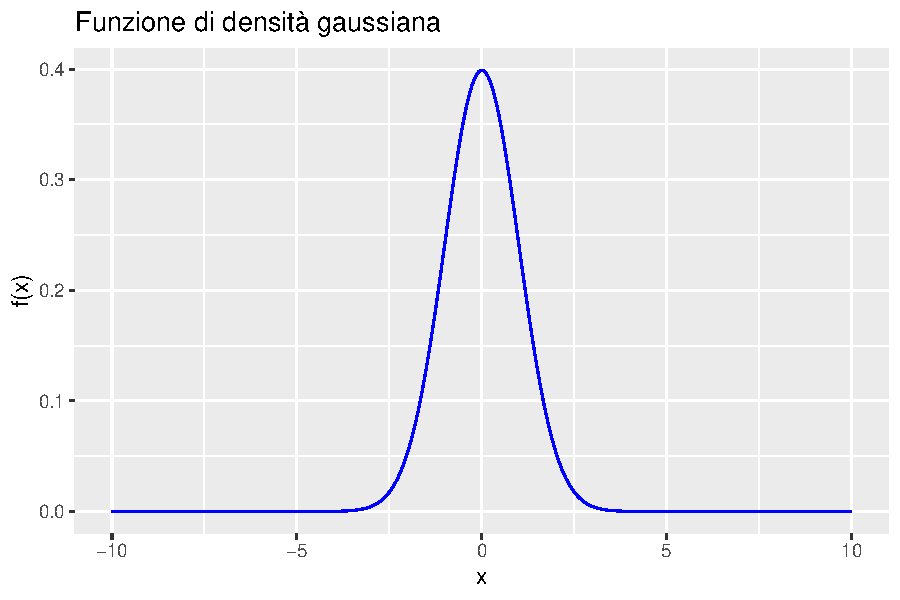
\includegraphics[keepaspectratio]{chapters/appendix/a15_calculus_files/figure-pdf/unnamed-chunk-3-1.pdf}}

Creiamo una funzione per approssimare l'integrale sommando i prodotti
\(\Delta x \cdot f(x)\):

\begin{Shaded}
\begin{Highlighting}[]
\NormalTok{integral\_approximation }\OtherTok{\textless{}{-}} \ControlFlowTok{function}\NormalTok{(f, a, b, n) \{}
\NormalTok{  delta }\OtherTok{\textless{}{-}}\NormalTok{ (b }\SpecialCharTok{{-}}\NormalTok{ a) }\SpecialCharTok{/}\NormalTok{ n}
  \FunctionTok{sum}\NormalTok{(delta }\SpecialCharTok{*}\NormalTok{ f)}
\NormalTok{\}}

\CommentTok{\# Calcolo dell\textquotesingle{}integrale approssimato}
\NormalTok{approx }\OtherTok{\textless{}{-}} \FunctionTok{integral\_approximation}\NormalTok{(fx, a, b, n)}
\NormalTok{approx}
\end{Highlighting}
\end{Shaded}

\begin{verbatim}
[1] 0.9999
\end{verbatim}

Confrontiamo il risultato con il calcolo fornito dalla funzione
\texttt{integrate} di R:

\begin{Shaded}
\begin{Highlighting}[]
\FunctionTok{integrate}\NormalTok{(}
  \ControlFlowTok{function}\NormalTok{(x) }\FunctionTok{gaussian}\NormalTok{(x, mu, sigma),}
  \AttributeTok{lower =}\NormalTok{ a,}
  \AttributeTok{upper =}\NormalTok{ b}
\NormalTok{)}
\end{Highlighting}
\end{Shaded}

\begin{verbatim}
1 with absolute error < 7.4e-05
\end{verbatim}

Calcoliamo l'area sotto la curva in intervalli di interesse. Ad esempio,
per \([-1.96, 1.96]\), che corrisponde al 95\% dell'area nella
distribuzione normale standard:

\begin{Shaded}
\begin{Highlighting}[]
\NormalTok{a }\OtherTok{\textless{}{-}} \SpecialCharTok{{-}}\FloatTok{1.96}
\NormalTok{b }\OtherTok{\textless{}{-}} \FloatTok{1.96}
\NormalTok{x\_range }\OtherTok{\textless{}{-}} \FunctionTok{seq}\NormalTok{(a, b, }\AttributeTok{length.out =}\NormalTok{ n)}
\NormalTok{fx }\OtherTok{\textless{}{-}} \FunctionTok{gaussian}\NormalTok{(x\_range, mu, sigma)}

\NormalTok{approx }\OtherTok{\textless{}{-}} \FunctionTok{integral\_approximation}\NormalTok{(fx, a, b, n)}
\NormalTok{approx}
\end{Highlighting}
\end{Shaded}

\begin{verbatim}
[1] 0.9499321
\end{verbatim}

Confrontiamo con il risultato fornito da \texttt{integrate()}:

\begin{Shaded}
\begin{Highlighting}[]
\FunctionTok{integrate}\NormalTok{(}
  \ControlFlowTok{function}\NormalTok{(x) }\FunctionTok{gaussian}\NormalTok{(x, mu, sigma),}
  \AttributeTok{lower =}\NormalTok{ a,}
  \AttributeTok{upper =}\NormalTok{ b}
\NormalTok{)}
\end{Highlighting}
\end{Shaded}

\begin{verbatim}
0.9500042 with absolute error < 1e-11
\end{verbatim}

Verifichiamo l'area sotto la curva per \([-1, 1]\), che rappresenta
circa il 68\% dell'area totale:

\begin{Shaded}
\begin{Highlighting}[]
\NormalTok{a }\OtherTok{\textless{}{-}} \SpecialCharTok{{-}}\FloatTok{1.0}
\NormalTok{b }\OtherTok{\textless{}{-}} \FloatTok{1.0}
\NormalTok{x\_range }\OtherTok{\textless{}{-}} \FunctionTok{seq}\NormalTok{(a, b, }\AttributeTok{length.out =}\NormalTok{ n)}
\NormalTok{fx }\OtherTok{\textless{}{-}} \FunctionTok{gaussian}\NormalTok{(x\_range, mu, sigma)}

\NormalTok{approx }\OtherTok{\textless{}{-}} \FunctionTok{integral\_approximation}\NormalTok{(fx, a, b, n)}
\NormalTok{approx}
\end{Highlighting}
\end{Shaded}

\begin{verbatim}
[1] 0.6826696
\end{verbatim}

Confronto:

\begin{Shaded}
\begin{Highlighting}[]
\FunctionTok{integrate}\NormalTok{(}
  \ControlFlowTok{function}\NormalTok{(x) }\FunctionTok{gaussian}\NormalTok{(x, mu, sigma),}
  \AttributeTok{lower =}\NormalTok{ a,}
  \AttributeTok{upper =}\NormalTok{ b}
\NormalTok{)}
\end{Highlighting}
\end{Shaded}

\begin{verbatim}
0.6826895 with absolute error < 7.6e-15
\end{verbatim}

In sintesi, questo approccio dimostra come calcolare l'integrale di una
funzione di densità in un intervallo utilizzando sia un metodo
approssimativo basato sulla somma dei rettangoli sia il metodo numerico
integrato. In entrambi i casi, l'obiettivo è calcolare l'area sotto la
curva, che corrisponde all'integrale della funzione di densità.

\section{Potenze}\label{potenze}

Le potenze sono un'operazione matematica che rappresenta un prodotto
ripetuto. Si indicano generalmente come:

\[
a^n,
\]

dove:

\begin{itemize}
\tightlist
\item
  \(a\) è la \textbf{base},
\item
  \(n\) è l'\textbf{esponente}.
\end{itemize}

La potenza rappresenta il prodotto della base \(a\) ripetuto \(n\)
volte.

\subsection{Definizione di potenza}\label{definizione-di-potenza}

\[
a^n = \underbrace{a \cdot a \cdot \dots \cdot a}_{n \text{ fattori}} \quad \text{con } n \in \mathbb{N}.
\]

Ad esempio:

\begin{itemize}
\tightlist
\item
  \(2^3 = 2 \cdot 2 \cdot 2 = 8\),
\item
  \(3^4 = 3 \cdot 3 \cdot 3 \cdot 3 = 81\).
\end{itemize}

\begin{center}\rule{0.5\linewidth}{0.5pt}\end{center}

\subsection{Proprietà delle potenze}\label{proprietuxe0-delle-potenze}

\begin{enumerate}
\def\labelenumi{\arabic{enumi}.}
\item
  \textbf{Moltiplicazione di potenze con la stessa base}:

  \[
  a^m \cdot a^n = a^{m+n}
  \]

  \textbf{Esempio}: \(2^3 \cdot 2^2 = 2^{3+2} = 2^5 = 32\).
\item
  \textbf{Divisione di potenze con la stessa base}:

  \[
  \frac{a^m}{a^n} = a^{m-n}, \quad \text{con } m \geq n.
  \]

  \textbf{Esempio}: \(\frac{5^4}{5^2} = 5^{4-2} = 5^2 = 25\).
\item
  \textbf{Potenze di potenze}:

  \[
  (a^m)^n = a^{m \cdot n}.
  \]

  \textbf{Esempio}: \((3^2)^3 = 3^{2 \cdot 3} = 3^6 = 729\).
\item
  \textbf{Prodotto di potenze con basi diverse ma lo stesso esponente}:

  \[
  a^n \cdot b^n = (a \cdot b)^n.
  \]

  \textbf{Esempio}: \(2^3 \cdot 3^3 = (2 \cdot 3)^3 = 6^3 = 216\).
\item
  \textbf{Divisione di potenze con basi diverse ma lo stesso esponente}:

  \[
  \frac{a^n}{b^n} = \left(\frac{a}{b}\right)^n.
  \]

  \textbf{Esempio}:
  \(\frac{4^2}{2^2} = \left(\frac{4}{2}\right)^2 = 2^2 = 4\).
\item
  \textbf{Esponente zero}:

  \[
  a^0 = 1, \quad \text{con } a \neq 0.
  \]

  \textbf{Esempio}: \(5^0 = 1\).
\item
  \textbf{Esponente negativo}:

  \[
  a^{-n} = \frac{1}{a^n}.
  \]

  \textbf{Esempio}: \(2^{-3} = \frac{1}{2^3} = \frac{1}{8}\).
\item
  \textbf{Radice come potenza frazionaria}:

  \[
  a^{\frac{1}{n}} = \sqrt[n]{a}, \quad a^{\frac{m}{n}} = \sqrt[n]{a^m}.
  \]

  \textbf{Esempio}: \(8^{\frac{1}{3}} = \sqrt[3]{8} = 2\).
\end{enumerate}

\begin{center}\rule{0.5\linewidth}{0.5pt}\end{center}

\subsection{Esempi pratici}\label{esempi-pratici}

\begin{enumerate}
\def\labelenumi{\arabic{enumi}.}
\item
  \textbf{Calcolo semplice}:

  \[
  4^3 = 4 \cdot 4 \cdot 4 = 64.
  \]
\item
  \textbf{Utilizzo delle proprietà}:

  \[
  3^5 \cdot 3^2 = 3^{5+2} = 3^7 = 2187.
  \]
\item
  \textbf{Divisione}:

  \[
  \frac{6^4}{6^2} = 6^{4-2} = 6^2 = 36.
  \]
\item
  \textbf{Esponente negativo}:

  \[
  10^{-2} = \frac{1}{10^2} = \frac{1}{100} = 0.01.
  \]
\item
  \textbf{Radice come potenza}:

  \[
  16^{\frac{1}{2}} = \sqrt{16} = 4.
  \]
\end{enumerate}

\begin{center}\rule{0.5\linewidth}{0.5pt}\end{center}

\subsection{Nota sui numeri razionali e
reali}\label{nota-sui-numeri-razionali-e-reali}

\begin{itemize}
\tightlist
\item
  Le potenze con esponenti interi sono definite per ogni base.
\item
  Le potenze con esponenti frazionari o reali richiedono che la base sia
  positiva per evitare ambiguità.
\end{itemize}

\section{Logaritmi}\label{logaritmi}

Il logaritmo è una funzione matematica che risponde alla domanda:
``quante volte devo moltiplicare un certo numero (chiamato''base'') per
ottenere un altro numero?'' Matematicamente, questo è espresso come:

\[
\log_b(a) = x \iff b^x = a
\]

Ad esempio, \(\log_2(8) = 3\) perché \(2^3 = 8\).

Nel contesto dei logaritmi, i valori molto piccoli (compresi tra 0 e 1)
diventano più grandi (in termini assoluti) e negativi quando applichiamo
una funzione logaritmica. Questo è utile per stabilizzare i calcoli,
specialmente quando lavoriamo con prodotti di numeri molto piccoli che
potrebbero portare a problemi di underflow.

Per esempio:

\begin{itemize}
\tightlist
\item
  \(\log(1) = 0\)
\item
  \(\log(0.1) = -1\)
\item
  \(\log(0.01) = -2\)
\item
  \(\log(0.001) = -3\)
\end{itemize}

Come si può vedere, i valori assoluti dei logaritmi crescono man mano
che il numero originale si avvicina a zero.

Una delle proprietà più utili dei logaritmi è che consentono di
trasformare un prodotto in una somma:

\[
\log_b(a \times c) = \log_b(a) + \log_b(c)
\]

Questa proprietà è estremamente utile in calcoli complessi, come nella
statistica bayesiana, dove il prodotto di molte probabilità potrebbe
diventare un numero molto piccolo e causare problemi numerici.

Un'altra proprietà utile dei logaritmi è che un rapporto tra due numeri
diventa la differenza dei loro logaritmi:

\[
\log_b\left(\frac{a}{c}\right) = \log_b(a) - \log_b(c)
\]

Anche questa proprietà è molto utilizzata in matematica, specialmente in
situazioni in cui è necessario normalizzare i dati.

In sintesi, i logaritmi sono strumenti potenti per semplificare e
stabilizzare i calcoli matematici. Essi consentono di lavorare più
agevolmente con numeri molto grandi o molto piccoli e di trasformare
operazioni complesse come prodotti e divisioni in somme e differenze,
rendendo i calcoli più gestibili e meno inclini a errori numerici.

\end{definition}

\phantomsection\label{refs}
\begin{CSLReferences}{1}{0}
\bibitem[\citeproctext]{ref-blitzstein2019introduction}
Blitzstein, J. K., \& Hwang, J. (2019). \emph{Introduction to
probability}. CRC Press.

\bibitem[\citeproctext]{ref-chivers2024everything}
Chivers, T. (2024). \emph{Everything is predictable: How bayesian
statistics explain our world}. Simon; Schuster.

\bibitem[\citeproctext]{ref-domini2011combining}
Domini, F., \& Caudek, C. (2011). Combining image signals before
three-dimensional reconstruction: The intrinsic constraint model of cue
integration. In J. Trommershäuser, K. Körding, \& M. S. Landy (Eds.),
\emph{Sensory cue integration} (pp. 120--143). Oxford University Press.
\url{https://doi.org/10.1093/acprof:oso/9780195387247.003.0008}

\bibitem[\citeproctext]{ref-eysenck2007anxiety}
Eysenck, M. W., Derakshan, N., Santos, R., \& Calvo, M. G. (2007).
Anxiety and cognitive performance: Attentional control theory.
\emph{Emotion}, \emph{7}(2), 336--353.

\bibitem[\citeproctext]{ref-de2017theory}
Finetti, B. de. (1970). \emph{Teoria delle probabilità} (pp. VIII,
350--769). G. Einaudi.

\bibitem[\citeproctext]{ref-gelman1995bayesian}
Gelman, A., Carlin, J. B., Stern, H. S., Dunson, D. B., Vehtari, A., \&
Rubin, D. B. (2013). \emph{Bayesian data analysis} (3rd ed.). {Chapman
and Hall/CRC}.

\bibitem[\citeproctext]{ref-graham_concrete_1994}
Graham, R. L., Knuth, D. E., \& Patashnik, O. (1994). \emph{Concrete
mathematics: A foundation for computer science} (2nd ed.).
Addison-Wesley.

\bibitem[\citeproctext]{ref-griffiths2024bayesian}
Griffiths, T. L., Chater, N., \& Tenenbaum, J. B. (2024). \emph{Bayesian
models of cognition: Reverse engineering the mind}. MIT Press.

\bibitem[\citeproctext]{ref-heard2021introduction}
Heard, N. (2021). \emph{An introduction to bayesian inference, methods
and computation}. Springer.

\bibitem[\citeproctext]{ref-jackson2020relationship}
Jackson, E. G. (2020). The relationship between belief and credence.
\emph{Philosophy Compass}, \emph{15}(6), e12668.

\bibitem[\citeproctext]{ref-Johnson2022bayesrules}
Johnson, A. A., Ott, M., \& Dogucu, M. (2022). \emph{{Bayes Rules! An
Introduction to Bayesian Modeling with R}}. CRC Press.

\bibitem[\citeproctext]{ref-doing_bayesian_data_an}
Kruschke, J. (2014). \emph{Doing bayesian data analysis: {A} tutorial
with {R}, JAGS, and {Stan}}. Academic Press.

\bibitem[\citeproctext]{ref-McElreath_rethinking}
McElreath, R. (2020). \emph{Statistical rethinking: {A} {Bayesian}
course with examples in {R} and {Stan}} (2nd Edition). CRC Press.

\bibitem[\citeproctext]{ref-segal2025embracing}
Segal, A., Tiego, J., Parkes, L., Holmes, A. J., Marquand, A. F., \&
Fornito, A. (2025). Embracing variability in the search for biological
mechanisms of psychiatric illness. \emph{Trends in Cognitive Sciences},
\emph{29}(1), 85--99.

\bibitem[\citeproctext]{ref-spiegelhalter2024probability}
Spiegelhalter, D. (2024). Why probability probably doesn't exist (but it
is useful to act like it does). \emph{Nature}, \emph{636}(8043),
560--563.

\end{CSLReferences}




\end{document}
